% Options for packages loaded elsewhere
\PassOptionsToPackage{unicode}{hyperref}
\PassOptionsToPackage{hyphens}{url}
\PassOptionsToPackage{dvipsnames,svgnames,x11names}{xcolor}
%
\documentclass[
  letterpaper,
  DIV=11,
  numbers=noendperiod]{scrreprt}

\usepackage{amsmath,amssymb}
\usepackage{iftex}
\ifPDFTeX
  \usepackage[T1]{fontenc}
  \usepackage[utf8]{inputenc}
  \usepackage{textcomp} % provide euro and other symbols
\else % if luatex or xetex
  \usepackage{unicode-math}
  \defaultfontfeatures{Scale=MatchLowercase}
  \defaultfontfeatures[\rmfamily]{Ligatures=TeX,Scale=1}
\fi
\usepackage{lmodern}
\ifPDFTeX\else  
    % xetex/luatex font selection
\fi
% Use upquote if available, for straight quotes in verbatim environments
\IfFileExists{upquote.sty}{\usepackage{upquote}}{}
\IfFileExists{microtype.sty}{% use microtype if available
  \usepackage[]{microtype}
  \UseMicrotypeSet[protrusion]{basicmath} % disable protrusion for tt fonts
}{}
\makeatletter
\@ifundefined{KOMAClassName}{% if non-KOMA class
  \IfFileExists{parskip.sty}{%
    \usepackage{parskip}
  }{% else
    \setlength{\parindent}{0pt}
    \setlength{\parskip}{6pt plus 2pt minus 1pt}}
}{% if KOMA class
  \KOMAoptions{parskip=half}}
\makeatother
\usepackage{xcolor}
\setlength{\emergencystretch}{3em} % prevent overfull lines
\setcounter{secnumdepth}{5}
% Make \paragraph and \subparagraph free-standing
\ifx\paragraph\undefined\else
  \let\oldparagraph\paragraph
  \renewcommand{\paragraph}[1]{\oldparagraph{#1}\mbox{}}
\fi
\ifx\subparagraph\undefined\else
  \let\oldsubparagraph\subparagraph
  \renewcommand{\subparagraph}[1]{\oldsubparagraph{#1}\mbox{}}
\fi

\usepackage{color}
\usepackage{fancyvrb}
\newcommand{\VerbBar}{|}
\newcommand{\VERB}{\Verb[commandchars=\\\{\}]}
\DefineVerbatimEnvironment{Highlighting}{Verbatim}{commandchars=\\\{\}}
% Add ',fontsize=\small' for more characters per line
\usepackage{framed}
\definecolor{shadecolor}{RGB}{241,243,245}
\newenvironment{Shaded}{\begin{snugshade}}{\end{snugshade}}
\newcommand{\AlertTok}[1]{\textcolor[rgb]{0.68,0.00,0.00}{#1}}
\newcommand{\AnnotationTok}[1]{\textcolor[rgb]{0.37,0.37,0.37}{#1}}
\newcommand{\AttributeTok}[1]{\textcolor[rgb]{0.40,0.45,0.13}{#1}}
\newcommand{\BaseNTok}[1]{\textcolor[rgb]{0.68,0.00,0.00}{#1}}
\newcommand{\BuiltInTok}[1]{\textcolor[rgb]{0.00,0.23,0.31}{#1}}
\newcommand{\CharTok}[1]{\textcolor[rgb]{0.13,0.47,0.30}{#1}}
\newcommand{\CommentTok}[1]{\textcolor[rgb]{0.37,0.37,0.37}{#1}}
\newcommand{\CommentVarTok}[1]{\textcolor[rgb]{0.37,0.37,0.37}{\textit{#1}}}
\newcommand{\ConstantTok}[1]{\textcolor[rgb]{0.56,0.35,0.01}{#1}}
\newcommand{\ControlFlowTok}[1]{\textcolor[rgb]{0.00,0.23,0.31}{#1}}
\newcommand{\DataTypeTok}[1]{\textcolor[rgb]{0.68,0.00,0.00}{#1}}
\newcommand{\DecValTok}[1]{\textcolor[rgb]{0.68,0.00,0.00}{#1}}
\newcommand{\DocumentationTok}[1]{\textcolor[rgb]{0.37,0.37,0.37}{\textit{#1}}}
\newcommand{\ErrorTok}[1]{\textcolor[rgb]{0.68,0.00,0.00}{#1}}
\newcommand{\ExtensionTok}[1]{\textcolor[rgb]{0.00,0.23,0.31}{#1}}
\newcommand{\FloatTok}[1]{\textcolor[rgb]{0.68,0.00,0.00}{#1}}
\newcommand{\FunctionTok}[1]{\textcolor[rgb]{0.28,0.35,0.67}{#1}}
\newcommand{\ImportTok}[1]{\textcolor[rgb]{0.00,0.46,0.62}{#1}}
\newcommand{\InformationTok}[1]{\textcolor[rgb]{0.37,0.37,0.37}{#1}}
\newcommand{\KeywordTok}[1]{\textcolor[rgb]{0.00,0.23,0.31}{#1}}
\newcommand{\NormalTok}[1]{\textcolor[rgb]{0.00,0.23,0.31}{#1}}
\newcommand{\OperatorTok}[1]{\textcolor[rgb]{0.37,0.37,0.37}{#1}}
\newcommand{\OtherTok}[1]{\textcolor[rgb]{0.00,0.23,0.31}{#1}}
\newcommand{\PreprocessorTok}[1]{\textcolor[rgb]{0.68,0.00,0.00}{#1}}
\newcommand{\RegionMarkerTok}[1]{\textcolor[rgb]{0.00,0.23,0.31}{#1}}
\newcommand{\SpecialCharTok}[1]{\textcolor[rgb]{0.37,0.37,0.37}{#1}}
\newcommand{\SpecialStringTok}[1]{\textcolor[rgb]{0.13,0.47,0.30}{#1}}
\newcommand{\StringTok}[1]{\textcolor[rgb]{0.13,0.47,0.30}{#1}}
\newcommand{\VariableTok}[1]{\textcolor[rgb]{0.07,0.07,0.07}{#1}}
\newcommand{\VerbatimStringTok}[1]{\textcolor[rgb]{0.13,0.47,0.30}{#1}}
\newcommand{\WarningTok}[1]{\textcolor[rgb]{0.37,0.37,0.37}{\textit{#1}}}

\providecommand{\tightlist}{%
  \setlength{\itemsep}{0pt}\setlength{\parskip}{0pt}}\usepackage{longtable,booktabs,array}
\usepackage{calc} % for calculating minipage widths
% Correct order of tables after \paragraph or \subparagraph
\usepackage{etoolbox}
\makeatletter
\patchcmd\longtable{\par}{\if@noskipsec\mbox{}\fi\par}{}{}
\makeatother
% Allow footnotes in longtable head/foot
\IfFileExists{footnotehyper.sty}{\usepackage{footnotehyper}}{\usepackage{footnote}}
\makesavenoteenv{longtable}
\usepackage{graphicx}
\makeatletter
\def\maxwidth{\ifdim\Gin@nat@width>\linewidth\linewidth\else\Gin@nat@width\fi}
\def\maxheight{\ifdim\Gin@nat@height>\textheight\textheight\else\Gin@nat@height\fi}
\makeatother
% Scale images if necessary, so that they will not overflow the page
% margins by default, and it is still possible to overwrite the defaults
% using explicit options in \includegraphics[width, height, ...]{}
\setkeys{Gin}{width=\maxwidth,height=\maxheight,keepaspectratio}
% Set default figure placement to htbp
\makeatletter
\def\fps@figure{htbp}
\makeatother
% definitions for citeproc citations
\NewDocumentCommand\citeproctext{}{}
\NewDocumentCommand\citeproc{mm}{%
  \begingroup\def\citeproctext{#2}\cite{#1}\endgroup}
\makeatletter
 % allow citations to break across lines
 \let\@cite@ofmt\@firstofone
 % avoid brackets around text for \cite:
 \def\@biblabel#1{}
 \def\@cite#1#2{{#1\if@tempswa , #2\fi}}
\makeatother
\newlength{\cslhangindent}
\setlength{\cslhangindent}{1.5em}
\newlength{\csllabelwidth}
\setlength{\csllabelwidth}{3em}
\newenvironment{CSLReferences}[2] % #1 hanging-indent, #2 entry-spacing
 {\begin{list}{}{%
  \setlength{\itemindent}{0pt}
  \setlength{\leftmargin}{0pt}
  \setlength{\parsep}{0pt}
  % turn on hanging indent if param 1 is 1
  \ifodd #1
   \setlength{\leftmargin}{\cslhangindent}
   \setlength{\itemindent}{-1\cslhangindent}
  \fi
  % set entry spacing
  \setlength{\itemsep}{#2\baselineskip}}}
 {\end{list}}
\usepackage{calc}
\newcommand{\CSLBlock}[1]{\hfill\break\parbox[t]{\linewidth}{\strut\ignorespaces#1\strut}}
\newcommand{\CSLLeftMargin}[1]{\parbox[t]{\csllabelwidth}{\strut#1\strut}}
\newcommand{\CSLRightInline}[1]{\parbox[t]{\linewidth - \csllabelwidth}{\strut#1\strut}}
\newcommand{\CSLIndent}[1]{\hspace{\cslhangindent}#1}

\KOMAoption{captions}{tableheading}
\makeatletter
\@ifpackageloaded{bookmark}{}{\usepackage{bookmark}}
\makeatother
\makeatletter
\@ifpackageloaded{caption}{}{\usepackage{caption}}
\AtBeginDocument{%
\ifdefined\contentsname
  \renewcommand*\contentsname{Table of contents}
\else
  \newcommand\contentsname{Table of contents}
\fi
\ifdefined\listfigurename
  \renewcommand*\listfigurename{List of Figures}
\else
  \newcommand\listfigurename{List of Figures}
\fi
\ifdefined\listtablename
  \renewcommand*\listtablename{List of Tables}
\else
  \newcommand\listtablename{List of Tables}
\fi
\ifdefined\figurename
  \renewcommand*\figurename{Figure}
\else
  \newcommand\figurename{Figure}
\fi
\ifdefined\tablename
  \renewcommand*\tablename{Table}
\else
  \newcommand\tablename{Table}
\fi
}
\@ifpackageloaded{float}{}{\usepackage{float}}
\floatstyle{ruled}
\@ifundefined{c@chapter}{\newfloat{codelisting}{h}{lop}}{\newfloat{codelisting}{h}{lop}[chapter]}
\floatname{codelisting}{Listing}
\newcommand*\listoflistings{\listof{codelisting}{List of Listings}}
\makeatother
\makeatletter
\makeatother
\makeatletter
\@ifpackageloaded{caption}{}{\usepackage{caption}}
\@ifpackageloaded{subcaption}{}{\usepackage{subcaption}}
\makeatother
\ifLuaTeX
  \usepackage{selnolig}  % disable illegal ligatures
\fi
\usepackage{bookmark}

\IfFileExists{xurl.sty}{\usepackage{xurl}}{} % add URL line breaks if available
\urlstyle{same} % disable monospaced font for URLs
\hypersetup{
  pdftitle={{[}Preregistration{]} Putting in the Effort: Modulation of Multimodal Effort in Communicative Breakdowns during a Gestural-Vocal Referential Game},
  colorlinks=true,
  linkcolor={blue},
  filecolor={Maroon},
  citecolor={Blue},
  urlcolor={Blue},
  pdfcreator={LaTeX via pandoc}}

\title{{[}Preregistration{]} Putting in the Effort: Modulation of
Multimodal Effort in Communicative Breakdowns during a Gestural-Vocal
Referential Game}
\author{}
\date{2025-07-11}

\begin{document}
\maketitle

\renewcommand*\contentsname{Table of contents}
{
\hypersetup{linkcolor=}
\setcounter{tocdepth}{2}
\tableofcontents
}
\bookmarksetup{startatroot}

\chapter*{Preface}\label{preface}
\addcontentsline{toc}{chapter}{Preface}

\markboth{Preface}{Preface}

This is a Quarto book.

\bookmarksetup{startatroot}

\chapter{Introduction}\label{introduction}

\bookmarksetup{startatroot}

\chapter{Introduction}\label{introduction-1}

\begin{Shaded}
\begin{Highlighting}[]
\ImportTok{import}\NormalTok{ sys}
\BuiltInTok{print}\NormalTok{(sys.executable)}
\end{Highlighting}
\end{Shaded}

\begin{verbatim}
C:\Users\kadava\AppData\Local\anaconda3\envs\TSprocess\python.exe
\end{verbatim}

This is a book created from markdown and executable code.

See Knuth (1984) for additional discussion of literate programming.

\bookmarksetup{startatroot}

\chapter{Processing I: from XDF to raw
files}\label{processing-i-from-xdf-to-raw-files}

Data for this experiment has been collected been collected using
LabStreamLayer, allowing for recording of precisely synchronized streams
(see \href{https://github.com/sccn/labstreaminglayer}{documentation}).

These streams include: - Audio stream (16kHz) - Webcam Frame stream (ca.
60 Hz) - Marker stream (sent from custom buttonbox) - Balance board
stream (500 Hz)

LSL outputs single file in Extensible Data Format (XDF). This file
contains all the data streams in form of a timeseries. In this script,
we extract all the streams from the file and create raw (audio, video,
and other) files for further processing.

Additionally, in this script, we - correct faulty delimitations of
trials - align 16kHz LSL audio and external 48kHz audio that has been
recorded outside of LSL, and cut this aligned audio to trial-sized files
- combine video and audio into single file

More information about the complete lab setup can be found in our
previous preregistration where we archived list of all equipment and
software used in the experiment. It is available here:
\url{https://osf.io/3nygq/}

\begin{Shaded}
\begin{Highlighting}[]
\CommentTok{\# import packages}
\ImportTok{import}\NormalTok{ os}
\ImportTok{import}\NormalTok{ pyxdf}
\ImportTok{import}\NormalTok{ glob}
\ImportTok{import}\NormalTok{ pandas }\ImportTok{as}\NormalTok{ pd}
\ImportTok{import}\NormalTok{ numpy }\ImportTok{as}\NormalTok{ np}
\ImportTok{import}\NormalTok{ wave, struct, random}
\ImportTok{from}\NormalTok{ scipy.io }\ImportTok{import}\NormalTok{ wavfile}
\ImportTok{import}\NormalTok{ noisereduce }\ImportTok{as}\NormalTok{ nr}
\ImportTok{import}\NormalTok{ cv2}
\ImportTok{import}\NormalTok{ matplotlib.pyplot }\ImportTok{as}\NormalTok{ plt}
\ImportTok{from}\NormalTok{ IPython.display }\ImportTok{import}\NormalTok{ Audio, Video}
\ImportTok{import}\NormalTok{ tempfile}
\ImportTok{import}\NormalTok{ subprocess}


\CommentTok{\# Set folders}
\NormalTok{curfolder }\OperatorTok{=}\NormalTok{ os.getcwd()}

\CommentTok{\# If folder data doesn\textquotesingle{}t exist, create it}
\ControlFlowTok{if} \KeywordTok{not}\NormalTok{ os.path.exists(curfolder}\OperatorTok{+}\StringTok{\textquotesingle{}}\CharTok{\textbackslash{}\textbackslash{}}\StringTok{data}\CharTok{\textbackslash{}\textbackslash{}}\StringTok{\textquotesingle{}}\NormalTok{):}
\NormalTok{    os.makedirs(curfolder}\OperatorTok{+}\StringTok{\textquotesingle{}}\CharTok{\textbackslash{}\textbackslash{}}\StringTok{data}\CharTok{\textbackslash{}\textbackslash{}}\StringTok{\textquotesingle{}}\NormalTok{)}
\NormalTok{datafolder }\OperatorTok{=}\NormalTok{ curfolder}\OperatorTok{+}\StringTok{\textquotesingle{}}\CharTok{\textbackslash{}\textbackslash{}}\StringTok{data}\CharTok{\textbackslash{}\textbackslash{}}\StringTok{\textquotesingle{}}

\CommentTok{\# Also error\_logs}
\ControlFlowTok{if} \KeywordTok{not}\NormalTok{ os.path.exists(datafolder}\OperatorTok{+}\StringTok{\textquotesingle{}}\CharTok{\textbackslash{}\textbackslash{}}\StringTok{error\_logs}\CharTok{\textbackslash{}\textbackslash{}}\StringTok{\textquotesingle{}}\NormalTok{):}
\NormalTok{    os.makedirs(datafolder}\OperatorTok{+}\StringTok{\textquotesingle{}}\CharTok{\textbackslash{}\textbackslash{}}\StringTok{error\_logs}\CharTok{\textbackslash{}\textbackslash{}}\StringTok{\textquotesingle{}}\NormalTok{)}
\NormalTok{errorlogs }\OperatorTok{=}\NormalTok{ datafolder}\OperatorTok{+}\StringTok{\textquotesingle{}}\CharTok{\textbackslash{}\textbackslash{}}\StringTok{error\_logs}\CharTok{\textbackslash{}\textbackslash{}}\StringTok{\textquotesingle{}}

\NormalTok{experiment\_to\_process }\OperatorTok{=}\NormalTok{ curfolder }\OperatorTok{+} \StringTok{\textquotesingle{}}\CharTok{\textbackslash{}\textbackslash{}}\StringTok{..}\CharTok{\textbackslash{}\textbackslash{}}\StringTok{00\_RAWDATA}\CharTok{\textbackslash{}\textbackslash{}}\StringTok{\textquotesingle{}}

\CommentTok{\# Also CsvDataTS\_raw}
\ControlFlowTok{if} \KeywordTok{not}\NormalTok{ os.path.exists(datafolder}\OperatorTok{+}\StringTok{\textquotesingle{}}\CharTok{\textbackslash{}\textbackslash{}}\StringTok{Data\_processed}\CharTok{\textbackslash{}\textbackslash{}}\StringTok{CsvDataTS\_raw}\CharTok{\textbackslash{}\textbackslash{}}\StringTok{\textquotesingle{}}\NormalTok{):}
\NormalTok{    os.makedirs(datafolder}\OperatorTok{+}\StringTok{\textquotesingle{}}\CharTok{\textbackslash{}\textbackslash{}}\StringTok{Data\_processed}\CharTok{\textbackslash{}\textbackslash{}}\StringTok{CsvDataTS\_raw}\CharTok{\textbackslash{}\textbackslash{}}\StringTok{\textquotesingle{}}\NormalTok{)}
\NormalTok{outputfolder }\OperatorTok{=}\NormalTok{ datafolder}\OperatorTok{+}\StringTok{\textquotesingle{}}\CharTok{\textbackslash{}\textbackslash{}}\StringTok{Data\_processed}\CharTok{\textbackslash{}\textbackslash{}}\StringTok{CsvDataTS\_raw}\CharTok{\textbackslash{}\textbackslash{}}\StringTok{\textquotesingle{}} \CommentTok{\# outputfolder raw}

\CommentTok{\# Audio in}
\ControlFlowTok{if} \KeywordTok{not}\NormalTok{ os.path.exists(datafolder}\OperatorTok{+}\StringTok{\textquotesingle{}}\CharTok{\textbackslash{}\textbackslash{}}\StringTok{Data\_processed}\CharTok{\textbackslash{}\textbackslash{}}\StringTok{CsvDataTS\_raw}\CharTok{\textbackslash{}\textbackslash{}}\StringTok{Audio}\CharTok{\textbackslash{}\textbackslash{}}\StringTok{\textquotesingle{}}\NormalTok{):}
\NormalTok{    os.makedirs(datafolder}\OperatorTok{+}\StringTok{\textquotesingle{}}\CharTok{\textbackslash{}\textbackslash{}}\StringTok{Data\_processed}\CharTok{\textbackslash{}\textbackslash{}}\StringTok{CsvDataTS\_raw}\CharTok{\textbackslash{}\textbackslash{}}\StringTok{Audio}\CharTok{\textbackslash{}\textbackslash{}}\StringTok{\textquotesingle{}}\NormalTok{)}

\CommentTok{\# Also Data\_trials}
\ControlFlowTok{if} \KeywordTok{not}\NormalTok{ os.path.exists(datafolder}\OperatorTok{+}\StringTok{\textquotesingle{}}\CharTok{\textbackslash{}\textbackslash{}}\StringTok{Data\_processed}\CharTok{\textbackslash{}\textbackslash{}}\StringTok{Data\_trials}\CharTok{\textbackslash{}\textbackslash{}}\StringTok{\textquotesingle{}}\NormalTok{):}
\NormalTok{    os.makedirs(datafolder}\OperatorTok{+}\StringTok{\textquotesingle{}}\CharTok{\textbackslash{}\textbackslash{}}\StringTok{Data\_processed}\CharTok{\textbackslash{}\textbackslash{}}\StringTok{Data\_trials}\CharTok{\textbackslash{}\textbackslash{}}\StringTok{\textquotesingle{}}\NormalTok{)}
\NormalTok{trialfolder }\OperatorTok{=}\NormalTok{ datafolder}\OperatorTok{+}\StringTok{\textquotesingle{}}\CharTok{\textbackslash{}\textbackslash{}}\StringTok{Data\_processed}\CharTok{\textbackslash{}\textbackslash{}}\StringTok{Data\_trials}\CharTok{\textbackslash{}\textbackslash{}}\StringTok{\textquotesingle{}} \CommentTok{\# outputfolder trialbased}


\CommentTok{\# Add audio in}
\ControlFlowTok{if} \KeywordTok{not}\NormalTok{ os.path.exists(datafolder}\OperatorTok{+}\StringTok{\textquotesingle{}}\CharTok{\textbackslash{}\textbackslash{}}\StringTok{Data\_processed}\CharTok{\textbackslash{}\textbackslash{}}\StringTok{Data\_trials}\CharTok{\textbackslash{}\textbackslash{}}\StringTok{Audio}\CharTok{\textbackslash{}\textbackslash{}}\StringTok{\textquotesingle{}}\NormalTok{):}
\NormalTok{    os.makedirs(datafolder}\OperatorTok{+}\StringTok{\textquotesingle{}}\CharTok{\textbackslash{}\textbackslash{}}\StringTok{Data\_processed}\CharTok{\textbackslash{}\textbackslash{}}\StringTok{Data\_trials}\CharTok{\textbackslash{}\textbackslash{}}\StringTok{Audio}\CharTok{\textbackslash{}\textbackslash{}}\StringTok{\textquotesingle{}}\NormalTok{)}

\CommentTok{\# Get all the folders in the target folder}
\NormalTok{datafolders }\OperatorTok{=}\NormalTok{ glob.glob(experiment\_to\_process}\OperatorTok{+}\StringTok{\textquotesingle{}*}\CharTok{\textbackslash{}\textbackslash{}}\StringTok{\textquotesingle{}}\NormalTok{)}

\CommentTok{\# Extract the folder IDs}
\NormalTok{datafolders\_id }\OperatorTok{=}\NormalTok{ [x.split(}\StringTok{\textquotesingle{}}\CharTok{\textbackslash{}\textbackslash{}}\StringTok{\textquotesingle{}}\NormalTok{)[}\OperatorTok{{-}}\DecValTok{2}\NormalTok{] }\ControlFlowTok{for}\NormalTok{ x }\KeywordTok{in}\NormalTok{ datafolders]}
\CommentTok{\# Ignore Demographics}
\NormalTok{datafolders\_id }\OperatorTok{=}\NormalTok{ [x }\ControlFlowTok{for}\NormalTok{ x }\KeywordTok{in}\NormalTok{ datafolders\_id }\ControlFlowTok{if} \StringTok{\textquotesingle{}Demographics\textquotesingle{}} \KeywordTok{not} \KeywordTok{in}\NormalTok{ x]}

\CommentTok{\# print(curfolder)}
\CommentTok{\# print(targetfolder)}


\CommentTok{\# Identify all xdf files and all the associated triallist info}
\NormalTok{xdffiles }\OperatorTok{=}\NormalTok{ []}
\NormalTok{trialdatas }\OperatorTok{=}\NormalTok{ []}

\ControlFlowTok{for}\NormalTok{ i }\KeywordTok{in}\NormalTok{ datafolders\_id:}
    \BuiltInTok{file} \OperatorTok{=}\NormalTok{ glob.glob(experiment\_to\_process}\OperatorTok{+}\NormalTok{i}\OperatorTok{+}\StringTok{\textquotesingle{}}\CharTok{\textbackslash{}\textbackslash{}}\StringTok{*.xdf\textquotesingle{}}\NormalTok{)}
\NormalTok{    trialfile }\OperatorTok{=}\NormalTok{ experiment\_to\_process}\OperatorTok{+}\NormalTok{i}\OperatorTok{+}\StringTok{\textquotesingle{}}\CharTok{\textbackslash{}\textbackslash{}}\StringTok{\textquotesingle{}}\OperatorTok{+}\NormalTok{i}\OperatorTok{+}\StringTok{\textquotesingle{}\_results\textquotesingle{}}\OperatorTok{+}\StringTok{\textquotesingle{}.csv\textquotesingle{}}
\NormalTok{    trialdatas.append(trialfile)}
\NormalTok{    xdffiles.extend(}\BuiltInTok{file}\NormalTok{)}
\end{Highlighting}
\end{Shaded}

\bookmarksetup{startatroot}

\chapter{Extracting streams from XDF
file}\label{extracting-streams-from-xdf-file}

Using \texttt{pyxdf} package, we can extract the streams from the XDF
file.

First, we extract streams for the whole recording session such that we
end up with a file per each stream that represents the whole timeseries
from the start to the end of the recording.

Then, we cut the whole streams into trial-sized chunks using the marker
stream.Marker stream is saving presses from button box that has been
administered by the experimentor. The presses indicates the start and
end of each trial. We also collect the trial start and end time via the
PsychoPy custom script that is used to run the experiment. We use this
information to connect the marker to the trial metadata such as - what
kind of concept is being performed - is this trial baselina, correction
1, correction 2 - who performs this trial - in which modality is this
trial

(Note that this code takes some time to execute.)

\begin{Shaded}
\begin{Highlighting}[]
\CommentTok{\# Audio write function}
\KeywordTok{def}\NormalTok{ to\_audio(fileloc, timeseries, samplerate }\OperatorTok{=} \DecValTok{16000}\NormalTok{, channels }\OperatorTok{=} \DecValTok{1}\NormalTok{):}
\NormalTok{    obj }\OperatorTok{=}\NormalTok{ wave.}\BuiltInTok{open}\NormalTok{(fileloc,}\StringTok{\textquotesingle{}w\textquotesingle{}}\NormalTok{)}
\NormalTok{    obj.setnchannels(channels) }\CommentTok{\# mono}
\NormalTok{    obj.setsampwidth(}\DecValTok{2}\NormalTok{)}
\NormalTok{    obj.setframerate(}\BuiltInTok{float}\NormalTok{(samplerate))}
    \ControlFlowTok{for}\NormalTok{ i }\KeywordTok{in}\NormalTok{ timeseries:}
\NormalTok{        data }\OperatorTok{=}\NormalTok{ struct.pack(}\StringTok{\textquotesingle{}\textless{}h\textquotesingle{}}\NormalTok{, }\BuiltInTok{int}\NormalTok{(i[}\DecValTok{0}\NormalTok{]))}
\NormalTok{        obj.writeframesraw( data )}
\NormalTok{    obj.close()}

\CommentTok{\# Function to retrieve closest value}
\KeywordTok{def}\NormalTok{ find\_closest\_value\_and\_retrieve(df, target\_number, target\_column, retrieve\_column):}
    \CommentTok{\# Get the absolute differences between a value in column and the target number}
\NormalTok{    differences }\OperatorTok{=} \BuiltInTok{abs}\NormalTok{(df[target\_column] }\OperatorTok{{-}}\NormalTok{ target\_number)}
    
    \CommentTok{\# Find the index of the minimum difference}
\NormalTok{    min\_difference\_index }\OperatorTok{=}\NormalTok{ differences.idxmin()}
    
    \CommentTok{\# Retrieve the corresponding value from the column}
\NormalTok{    result\_value }\OperatorTok{=}\NormalTok{ df.loc[min\_difference\_index, retrieve\_column]}

    \ControlFlowTok{return}\NormalTok{ result\_value}

\KeywordTok{def}\NormalTok{ write\_video(vidloc, fourcc, originalfps, frameWidth, frameHeight, capture, frames):}
\NormalTok{    out }\OperatorTok{=}\NormalTok{ cv2.VideoWriter(vidloc, fourcc, fps }\OperatorTok{=}\NormalTok{ originalfps, frameSize }\OperatorTok{=}\NormalTok{ (}\BuiltInTok{int}\NormalTok{(frameWidth), }\BuiltInTok{int}\NormalTok{(frameHeight)))}
    \CommentTok{\#print(\textquotesingle{}Looping over frames\textquotesingle{})}

    \CommentTok{\# index the frames of the current trial }
    \ControlFlowTok{for}\NormalTok{ fra }\KeywordTok{in}\NormalTok{ frames:}
\NormalTok{        capture.}\BuiltInTok{set}\NormalTok{(cv2.CAP\_PROP\_POS\_FRAMES, fra)}
\NormalTok{        ret, frame }\OperatorTok{=}\NormalTok{ capture.read()}
        \ControlFlowTok{if}\NormalTok{ ret:}
\NormalTok{            out.write(frame)}
            
        \ControlFlowTok{if} \KeywordTok{not}\NormalTok{ ret:}
            \BuiltInTok{print}\NormalTok{(}\StringTok{\textquotesingle{}a frame was dropped: \textquotesingle{}} \OperatorTok{+} \BuiltInTok{str}\NormalTok{(fra))}
        
\NormalTok{    capture.release()}
\NormalTok{    out.release()}
\end{Highlighting}
\end{Shaded}

\begin{Shaded}
\begin{Highlighting}[]
\NormalTok{errorlist }\OperatorTok{=}\NormalTok{ []}

\ControlFlowTok{for}\NormalTok{ dat }\KeywordTok{in}\NormalTok{ datafolders\_id:}
    \BuiltInTok{print}\NormalTok{(}\StringTok{\textquotesingle{}Loading in data from participant: \textquotesingle{}} \OperatorTok{+}\NormalTok{ dat)}
\NormalTok{    trialdata }\OperatorTok{=}\NormalTok{ pd.read\_csv(experiment\_to\_process}\OperatorTok{+}\NormalTok{dat}\OperatorTok{+}\StringTok{\textquotesingle{}}\CharTok{\textbackslash{}\textbackslash{}}\StringTok{\textquotesingle{}}\OperatorTok{+}\NormalTok{dat}\OperatorTok{+}\StringTok{\textquotesingle{}\_results.csv\textquotesingle{}}\NormalTok{, sep}\OperatorTok{=}\StringTok{","}\NormalTok{)}
    \CommentTok{\#print(trialdata)}
    
    \CommentTok{\# Get the xdf file}
\NormalTok{    files }\OperatorTok{=}\NormalTok{ glob.glob(experiment\_to\_process}\OperatorTok{+}\NormalTok{dat}\OperatorTok{+}\StringTok{\textquotesingle{}}\CharTok{\textbackslash{}\textbackslash{}}\StringTok{*.xdf\textquotesingle{}}\NormalTok{)}
\NormalTok{    streams, header }\OperatorTok{=}\NormalTok{ pyxdf.load\_xdf(files[}\DecValTok{0}\NormalTok{])   }
    \CommentTok{\# We go through each stream and save it as a csv}
    \ControlFlowTok{for}\NormalTok{ stream }\KeywordTok{in}\NormalTok{ streams:}
\NormalTok{        timeseriestype }\OperatorTok{=}\NormalTok{ stream[}\StringTok{\textquotesingle{}info\textquotesingle{}}\NormalTok{][}\StringTok{\textquotesingle{}name\textquotesingle{}}\NormalTok{][}\DecValTok{0}\NormalTok{]}
        \BuiltInTok{print}\NormalTok{(timeseriestype)}
\NormalTok{        samplerate }\OperatorTok{=} \BuiltInTok{round}\NormalTok{(}\BuiltInTok{float}\NormalTok{(stream[}\StringTok{\textquotesingle{}info\textquotesingle{}}\NormalTok{][}\StringTok{\textquotesingle{}nominal\_srate\textquotesingle{}}\NormalTok{][}\DecValTok{0}\NormalTok{]))}
        \CommentTok{\# In the xdf loop over the streams and save it as csv if not yet exists}
\NormalTok{        channelcount }\OperatorTok{=}\NormalTok{ stream[}\StringTok{\textquotesingle{}info\textquotesingle{}}\NormalTok{][}\StringTok{\textquotesingle{}channel\_count\textquotesingle{}}\NormalTok{][}\DecValTok{0}\NormalTok{]}
        \BuiltInTok{print}\NormalTok{(}\StringTok{\textquotesingle{}working on stream: \textquotesingle{}} \OperatorTok{+}\NormalTok{ timeseriestype }\OperatorTok{+} \StringTok{\textquotesingle{}  with a channel count of \textquotesingle{}} \OperatorTok{+} \BuiltInTok{str}\NormalTok{(channelcount) }\OperatorTok{+}\StringTok{\textquotesingle{}}\CharTok{\textbackslash{}n}\StringTok{ and a sampling rate of \textquotesingle{}} \OperatorTok{+} \BuiltInTok{str}\NormalTok{(samplerate))}
\NormalTok{        timevec }\OperatorTok{=}\NormalTok{ stream[}\StringTok{\textquotesingle{}time\_stamps\textquotesingle{}}\NormalTok{]}
\NormalTok{        timeseries }\OperatorTok{=}\NormalTok{ stream[}\StringTok{\textquotesingle{}time\_series\textquotesingle{}}\NormalTok{]}
\NormalTok{        matrix\_aux }\OperatorTok{=}\NormalTok{ np.vstack([np.transpose(timevec),np.transpose(timeseries)])}
\NormalTok{        matrix }\OperatorTok{=}\NormalTok{ np.transpose(matrix\_aux)}
\NormalTok{        df\_lab }\OperatorTok{=}\NormalTok{ pd.DataFrame(matrix)}
\NormalTok{        df\_lab.to\_csv(outputfolder}\OperatorTok{+}\NormalTok{dat}\OperatorTok{+}\StringTok{\textquotesingle{}\_\textquotesingle{}}\OperatorTok{+}\NormalTok{timeseriestype}\OperatorTok{+}\StringTok{\textquotesingle{}\_nominal\_srate\textquotesingle{}}\OperatorTok{+}\BuiltInTok{str}\NormalTok{(samplerate)}\OperatorTok{+}\StringTok{\textquotesingle{}.csv\textquotesingle{}}\NormalTok{,index}\OperatorTok{=}\VariableTok{False}\NormalTok{)}
        \CommentTok{\# For audio stream also create a wav file}
        \ControlFlowTok{if}\NormalTok{ timeseriestype }\OperatorTok{==} \StringTok{\textquotesingle{}Mic\textquotesingle{}}\NormalTok{:}
\NormalTok{            wavloc }\OperatorTok{=}\NormalTok{ outputfolder}\OperatorTok{+}\StringTok{\textquotesingle{}Audio/\textquotesingle{}}\OperatorTok{+}\NormalTok{dat}\OperatorTok{+}\StringTok{\textquotesingle{}\_\textquotesingle{}}\OperatorTok{+}\NormalTok{timeseriestype}\OperatorTok{+}\StringTok{\textquotesingle{}\_nominal\_srate\textquotesingle{}}\OperatorTok{+}\BuiltInTok{str}\NormalTok{(samplerate)}\OperatorTok{+}\StringTok{\textquotesingle{}.wav\textquotesingle{}}
\NormalTok{            to\_audio(wavloc, timeseries)}
            \CommentTok{\# Load data}
\NormalTok{            rate, data }\OperatorTok{=}\NormalTok{ wavfile.read(wavloc)}
            \CommentTok{\# Perform noise reduction}
\NormalTok{            reduced\_noise }\OperatorTok{=}\NormalTok{ nr.reduce\_noise(y}\OperatorTok{=}\NormalTok{data, sr}\OperatorTok{=}\NormalTok{rate, n\_std\_thresh\_stationary}\OperatorTok{=}\FloatTok{1.5}\NormalTok{,stationary}\OperatorTok{=}\VariableTok{True}\NormalTok{)}
\NormalTok{            wavloc2 }\OperatorTok{=}\NormalTok{ outputfolder}\OperatorTok{+}\StringTok{\textquotesingle{}Audio/\textquotesingle{}}\OperatorTok{+}\NormalTok{dat}\OperatorTok{+}\StringTok{\textquotesingle{}\_\textquotesingle{}}\OperatorTok{+}\NormalTok{timeseriestype}\OperatorTok{+}\StringTok{\textquotesingle{}\_nominal\_srate\textquotesingle{}}\OperatorTok{+}\BuiltInTok{str}\NormalTok{(samplerate)}\OperatorTok{+}\StringTok{\textquotesingle{}\_denoised.wav\textquotesingle{}}
\NormalTok{            wavfile.write(wavloc2, rate, reduced\_noise)}

        \BuiltInTok{print}\NormalTok{(}\StringTok{\textquotesingle{}done with processing a complete time series and audio data\textquotesingle{}}\NormalTok{)}
        \BuiltInTok{print}\NormalTok{(}\StringTok{\textquotesingle{}we will now start making trial snipped data\textquotesingle{}}\NormalTok{) }

        \CommentTok{\# Load MyMarkerStream}
\NormalTok{        markers }\OperatorTok{=}\NormalTok{ pd.read\_csv(outputfolder}\OperatorTok{+}\NormalTok{dat}\OperatorTok{+}\StringTok{\textquotesingle{}\_MyMarkerStream\_nominal\_srate0.csv\textquotesingle{}}\NormalTok{)}
        
        \CommentTok{\# Cut all timeseries to trial level based on the markers}
        \ControlFlowTok{if}\NormalTok{ timeseriestype }\OperatorTok{!=} \StringTok{\textquotesingle{}MyMarkerStream\textquotesingle{}}\NormalTok{:}
            
\NormalTok{            beginlist }\OperatorTok{=}\NormalTok{ []}
\NormalTok{            endlist }\OperatorTok{=}\NormalTok{ []}
\NormalTok{            timestamps }\OperatorTok{=}\NormalTok{ []}
\NormalTok{            timestamps\_2 }\OperatorTok{=}\NormalTok{ []}
\NormalTok{            tpose\_starts }\OperatorTok{=}\NormalTok{ []}
\NormalTok{            tpose\_ends }\OperatorTok{=}\NormalTok{ []}

            \CommentTok{\# Iterate over markers and save times of trial starts and ends}
            \ControlFlowTok{for}\NormalTok{ row }\KeywordTok{in}\NormalTok{ markers.iterrows():}
                \ControlFlowTok{if} \StringTok{\textquotesingle{}Trial\_start\textquotesingle{}} \KeywordTok{in}\NormalTok{ row[}\DecValTok{1}\NormalTok{].iloc[}\DecValTok{1}\NormalTok{] }\KeywordTok{or} \StringTok{\textquotesingle{}Practice trial starts\textquotesingle{}} \KeywordTok{in}\NormalTok{ row[}\DecValTok{1}\NormalTok{].iloc[}\DecValTok{1}\NormalTok{]:}
\NormalTok{                    beginlist.append(row[}\DecValTok{1}\NormalTok{].iloc[}\DecValTok{0}\NormalTok{])}
                \ControlFlowTok{if} \StringTok{\textquotesingle{}Trial\_end\textquotesingle{}} \KeywordTok{in}\NormalTok{ row[}\DecValTok{1}\NormalTok{].iloc[}\DecValTok{1}\NormalTok{] }\KeywordTok{or} \StringTok{\textquotesingle{}Practice trial ends\textquotesingle{}} \KeywordTok{in}\NormalTok{ row[}\DecValTok{1}\NormalTok{].iloc[}\DecValTok{1}\NormalTok{]:}
\NormalTok{                    endlist.append(row[}\DecValTok{1}\NormalTok{].iloc[}\DecValTok{0}\NormalTok{])}
                \ControlFlowTok{if} \StringTok{\textquotesingle{}Experiment\_start\textquotesingle{}} \KeywordTok{in}\NormalTok{ row[}\DecValTok{1}\NormalTok{].iloc[}\DecValTok{1}\NormalTok{]:}
\NormalTok{                    timestamps.append(row[}\DecValTok{1}\NormalTok{].iloc[}\DecValTok{0}\NormalTok{])}
                \ControlFlowTok{if} \StringTok{\textquotesingle{}New block starts\textquotesingle{}} \KeywordTok{in}\NormalTok{ row[}\DecValTok{1}\NormalTok{].iloc[}\DecValTok{1}\NormalTok{]:}
\NormalTok{                    timestamps\_2.append(row[}\DecValTok{1}\NormalTok{].iloc[}\DecValTok{0}\NormalTok{])}
                \ControlFlowTok{if} \StringTok{\textquotesingle{}Tpose starts\textquotesingle{}} \KeywordTok{in}\NormalTok{ row[}\DecValTok{1}\NormalTok{].iloc[}\DecValTok{1}\NormalTok{]:}
\NormalTok{                    tpose\_starts.append(row[}\DecValTok{1}\NormalTok{].iloc[}\DecValTok{0}\NormalTok{])}
                \ControlFlowTok{if} \StringTok{\textquotesingle{}Tpose ends\textquotesingle{}} \KeywordTok{in}\NormalTok{ row[}\DecValTok{1}\NormalTok{].iloc[}\DecValTok{1}\NormalTok{]:}
\NormalTok{                    tpose\_ends.append(row[}\DecValTok{1}\NormalTok{].iloc[}\DecValTok{0}\NormalTok{])}
                    
            \CommentTok{\# Converting coefficient for lsl to psychopy time}
\NormalTok{            exp\_start\_pp }\OperatorTok{=} \BuiltInTok{float}\NormalTok{(trialdata[}\StringTok{\textquotesingle{}exp\_start\textquotesingle{}}\NormalTok{][}\DecValTok{0}\NormalTok{])}
\NormalTok{            block\_start\_pp }\OperatorTok{=} \BuiltInTok{float}\NormalTok{(trialdata[}\StringTok{\textquotesingle{}block\_start\textquotesingle{}}\NormalTok{][}\DecValTok{0}\NormalTok{])}
            
            \CommentTok{\# Get to lsl\_to\_pp coefficient}
            \ControlFlowTok{if}\NormalTok{ timestamps }\OperatorTok{!=}\NormalTok{ []:}
\NormalTok{                lsl\_to\_pp }\OperatorTok{=}\NormalTok{ timestamps[}\DecValTok{0}\NormalTok{] }\OperatorTok{{-}}\NormalTok{ exp\_start\_pp}
            \ControlFlowTok{else}\NormalTok{:}
\NormalTok{                lsl\_to\_pp }\OperatorTok{=}\NormalTok{ timestamps\_2[}\DecValTok{0}\NormalTok{] }\OperatorTok{{-}}\NormalTok{ block\_start\_pp}
        
            \CommentTok{\# Now we can proceed to cutting   }
            \ControlFlowTok{for}\NormalTok{ i }\KeywordTok{in} \BuiltInTok{range}\NormalTok{(}\BuiltInTok{len}\NormalTok{(beginlist)):}
                \CommentTok{\# Prepare the range of the trial}
\NormalTok{                begin }\OperatorTok{=}\NormalTok{ beginlist[i]}
\NormalTok{                end }\OperatorTok{=}\NormalTok{ endlist[i]}
\NormalTok{                indices }\OperatorTok{=}\NormalTok{ (df\_lab.loc[:,}\DecValTok{0}\NormalTok{] }\OperatorTok{\textgreater{}}\NormalTok{ begin) }\OperatorTok{\&}\NormalTok{ (df\_lab.loc[:,}\DecValTok{0}\NormalTok{] }\OperatorTok{\textless{}}\NormalTok{ end)}
\NormalTok{                beginst }\OperatorTok{=} \BuiltInTok{min}\NormalTok{(df\_lab.loc[:,}\DecValTok{0}\NormalTok{]) }\CommentTok{\# start time of the timeseries}
\NormalTok{                endst }\OperatorTok{=} \BuiltInTok{max}\NormalTok{(df\_lab.loc[:,}\DecValTok{0}\NormalTok{])  }\CommentTok{\# end time of the timeseries}
\NormalTok{                subset }\OperatorTok{=}\NormalTok{ df\_lab.loc[indices, :]}
                \CommentTok{\# Convert the beginst to psychopy time}
\NormalTok{                beginst\_pp }\OperatorTok{=}\NormalTok{ begin }\OperatorTok{{-}}\NormalTok{ lsl\_to\_pp}
                \CommentTok{\# Now find in trialdata the closest time to the beginst\_pp to gather info}
                \CommentTok{\# Whether it is practice or trial}
\NormalTok{                practice }\OperatorTok{=}\NormalTok{ find\_closest\_value\_and\_retrieve(trialdata, beginst\_pp, }\StringTok{\textquotesingle{}trial\_start\textquotesingle{}}\NormalTok{, }\StringTok{\textquotesingle{}practice\textquotesingle{}}\NormalTok{)}
                \ControlFlowTok{if}\NormalTok{ practice }\OperatorTok{==} \StringTok{\textquotesingle{}practice\textquotesingle{}}\NormalTok{:}
\NormalTok{                    trialtype }\OperatorTok{=} \StringTok{\textquotesingle{}pr\textquotesingle{}}
                \ControlFlowTok{else}\NormalTok{:}
\NormalTok{                    trialtype }\OperatorTok{=} \StringTok{\textquotesingle{}trial\textquotesingle{}}
                
                \CommentTok{\# Which participant it is}
\NormalTok{                cycle }\OperatorTok{=}\NormalTok{ find\_closest\_value\_and\_retrieve(trialdata, beginst\_pp, }\StringTok{\textquotesingle{}trial\_start\textquotesingle{}}\NormalTok{, }\StringTok{\textquotesingle{}cycle\textquotesingle{}}\NormalTok{)}
                \ControlFlowTok{if}\NormalTok{ cycle }\OperatorTok{==} \DecValTok{0}\NormalTok{:}
\NormalTok{                    participant }\OperatorTok{=} \StringTok{\textquotesingle{}p0\textquotesingle{}}
                \ControlFlowTok{else}\NormalTok{:}
\NormalTok{                    participant }\OperatorTok{=} \StringTok{\textquotesingle{}p1\textquotesingle{}}

                \CommentTok{\# What concept it is}
\NormalTok{                word }\OperatorTok{=}\NormalTok{ find\_closest\_value\_and\_retrieve(trialdata, beginst\_pp, }\StringTok{\textquotesingle{}trial\_start\textquotesingle{}}\NormalTok{, }\StringTok{\textquotesingle{}word\textquotesingle{}}\NormalTok{)}
                \CommentTok{\# Modality}
\NormalTok{                modality }\OperatorTok{=}\NormalTok{ find\_closest\_value\_and\_retrieve(trialdata, beginst\_pp, }\StringTok{\textquotesingle{}trial\_start\textquotesingle{}}\NormalTok{, }\StringTok{\textquotesingle{}modality\textquotesingle{}}\NormalTok{)}
                \CommentTok{\# Correction, if applicable}
\NormalTok{                correction\_info }\OperatorTok{=}\NormalTok{ find\_closest\_value\_and\_retrieve(trialdata, beginst\_pp, }\StringTok{\textquotesingle{}trial\_start\textquotesingle{}}\NormalTok{, }\StringTok{\textquotesingle{}correction\textquotesingle{}}\NormalTok{)}
                \ControlFlowTok{if}\NormalTok{ correction\_info }\OperatorTok{==} \DecValTok{0}\NormalTok{:}
\NormalTok{                    correction }\OperatorTok{=} \StringTok{\textquotesingle{}\_c0\textquotesingle{}}
                \ControlFlowTok{elif}\NormalTok{ correction\_info }\OperatorTok{==} \DecValTok{1}\NormalTok{:}
\NormalTok{                    correction }\OperatorTok{=} \StringTok{\textquotesingle{}\_c1\textquotesingle{}}
                \ControlFlowTok{elif}\NormalTok{ correction\_info }\OperatorTok{==} \DecValTok{2}\NormalTok{:}
\NormalTok{                    correction }\OperatorTok{=} \StringTok{\textquotesingle{}\_c2\textquotesingle{}}
                \ControlFlowTok{else}\NormalTok{:}
\NormalTok{                    correction }\OperatorTok{=} \StringTok{\textquotesingle{}\textquotesingle{}}
                
                \CommentTok{\# Continue saving}
                \ControlFlowTok{if}\NormalTok{(}\BuiltInTok{len}\NormalTok{(subset.axes[}\DecValTok{0}\NormalTok{])}\OperatorTok{\textless{}}\DecValTok{2}\NormalTok{):}
\NormalTok{                    errorlist.append(dat }\OperatorTok{+} \StringTok{" for "}\OperatorTok{+}\NormalTok{ timeseriestype }\OperatorTok{+} \StringTok{" for trial "} \OperatorTok{+} \BuiltInTok{str}\NormalTok{(i) }\OperatorTok{+} \StringTok{\textquotesingle{}NO DATA WITHIN RANGE...\textquotesingle{}}\NormalTok{)}
                \ControlFlowTok{if}\NormalTok{(}\BuiltInTok{len}\NormalTok{(subset.axes[}\DecValTok{0}\NormalTok{])}\OperatorTok{\textgreater{}}\DecValTok{2}\NormalTok{):}
                     \CommentTok{\# Save subset to csv}
\NormalTok{                      subset.to\_csv(trialfolder}\OperatorTok{+}\NormalTok{dat}\OperatorTok{+}\StringTok{\textquotesingle{}\_\textquotesingle{}}\OperatorTok{+}\NormalTok{trialtype}\OperatorTok{+}\StringTok{\textquotesingle{}\_\textquotesingle{}}\OperatorTok{+} \BuiltInTok{str}\NormalTok{(i) }\OperatorTok{+}\StringTok{\textquotesingle{}\_\textquotesingle{}}\OperatorTok{+}\NormalTok{timeseriestype}\OperatorTok{+}\StringTok{\textquotesingle{}\_nominal\_srate\textquotesingle{}}\OperatorTok{+}\BuiltInTok{str}\NormalTok{(samplerate)}\OperatorTok{+}\StringTok{\textquotesingle{}\_\textquotesingle{}}\OperatorTok{+}\NormalTok{participant}\OperatorTok{+}\StringTok{\textquotesingle{}\_\textquotesingle{}}\OperatorTok{+}\NormalTok{word}\OperatorTok{+}\StringTok{\textquotesingle{}\_\textquotesingle{}}\OperatorTok{+}\NormalTok{modality}\OperatorTok{+}\NormalTok{correction}\OperatorTok{+}\StringTok{\textquotesingle{}.csv\textquotesingle{}}\NormalTok{, index}\OperatorTok{=}\VariableTok{False}\NormalTok{)}
                      \ControlFlowTok{if}\NormalTok{ timeseriestype }\OperatorTok{==} \StringTok{\textquotesingle{}Mic\textquotesingle{}}\NormalTok{:}
\NormalTok{                            wavloc }\OperatorTok{=}\NormalTok{ trialfolder}\OperatorTok{+}\StringTok{\textquotesingle{}Audio/\textquotesingle{}}\OperatorTok{+}\NormalTok{dat}\OperatorTok{+}\StringTok{\textquotesingle{}\_\textquotesingle{}}\OperatorTok{+}\NormalTok{trialtype}\OperatorTok{+}\StringTok{\textquotesingle{}\_\textquotesingle{}}\OperatorTok{+} \BuiltInTok{str}\NormalTok{(i) }\OperatorTok{+}\StringTok{\textquotesingle{}\_\textquotesingle{}}\OperatorTok{+}\NormalTok{timeseriestype}\OperatorTok{+}\StringTok{\textquotesingle{}\_nominal\_srate\textquotesingle{}}\OperatorTok{+}\BuiltInTok{str}\NormalTok{(samplerate)}\OperatorTok{+}\StringTok{\textquotesingle{}\_\textquotesingle{}}\OperatorTok{+}\NormalTok{participant}\OperatorTok{+}\StringTok{\textquotesingle{}\_\textquotesingle{}}\OperatorTok{+}\NormalTok{word}\OperatorTok{+}\StringTok{\textquotesingle{}\_\textquotesingle{}}\OperatorTok{+}\NormalTok{modality}\OperatorTok{+}\NormalTok{correction}\OperatorTok{+}\StringTok{\textquotesingle{}.wav\textquotesingle{}}
\NormalTok{                            to\_audio(wavloc, timeseries[indices])}
                          \CommentTok{\# Also apply denoising}
\NormalTok{                            reduced\_noiseclip }\OperatorTok{=}\NormalTok{ reduced\_noise[indices]}
\NormalTok{                            wavloc2 }\OperatorTok{=}\NormalTok{ trialfolder}\OperatorTok{+}\StringTok{\textquotesingle{}Audio/\textquotesingle{}}\OperatorTok{+}\NormalTok{dat}\OperatorTok{+}\StringTok{\textquotesingle{}\_\textquotesingle{}}\OperatorTok{+}\NormalTok{trialtype}\OperatorTok{+}\StringTok{\textquotesingle{}\_\textquotesingle{}}\OperatorTok{+} \BuiltInTok{str}\NormalTok{(i) }\OperatorTok{+}\StringTok{\textquotesingle{}\_\textquotesingle{}}\OperatorTok{+}\NormalTok{timeseriestype}\OperatorTok{+}\StringTok{\textquotesingle{}\_nominal\_srate\textquotesingle{}}\OperatorTok{+}\BuiltInTok{str}\NormalTok{(samplerate)}\OperatorTok{+}\StringTok{\textquotesingle{}\_\textquotesingle{}}\OperatorTok{+}\NormalTok{participant}\OperatorTok{+}\StringTok{\textquotesingle{}\_\textquotesingle{}}\OperatorTok{+}\NormalTok{word}\OperatorTok{+}\StringTok{\textquotesingle{}\_\textquotesingle{}}\OperatorTok{+}\NormalTok{modality}\OperatorTok{+}\NormalTok{correction}\OperatorTok{+}\StringTok{\textquotesingle{}\_denoised.wav\textquotesingle{}}
\NormalTok{                            wavfile.write(wavloc2, rate, reduced\_noiseclip)}
            
            \CommentTok{\# Get information about the tpose for camera}
            \ControlFlowTok{if}\NormalTok{ timeseriestype }\OperatorTok{==} \StringTok{\textquotesingle{}MyWebcamFrameStream\textquotesingle{}}\NormalTok{:}
                \ControlFlowTok{for}\NormalTok{ i }\KeywordTok{in} \BuiltInTok{range}\NormalTok{(}\BuiltInTok{len}\NormalTok{(tpose\_starts)):}
\NormalTok{                    begin }\OperatorTok{=}\NormalTok{ tpose\_starts[i]}
\NormalTok{                    end }\OperatorTok{=}\NormalTok{ tpose\_ends[i]}
\NormalTok{                    indices }\OperatorTok{=}\NormalTok{ (df\_lab.loc[:,}\DecValTok{0}\NormalTok{] }\OperatorTok{\textgreater{}}\NormalTok{ begin) }\OperatorTok{\&}\NormalTok{ (df\_lab.loc[:,}\DecValTok{0}\NormalTok{] }\OperatorTok{\textless{}}\NormalTok{ end)}
\NormalTok{                    beginst }\OperatorTok{=} \BuiltInTok{min}\NormalTok{(df\_lab.loc[:,}\DecValTok{0}\NormalTok{])}
\NormalTok{                    endst }\OperatorTok{=} \BuiltInTok{max}\NormalTok{(df\_lab.loc[:,}\DecValTok{0}\NormalTok{])}
\NormalTok{                    subset }\OperatorTok{=}\NormalTok{ df\_lab.loc[indices, :]}
                    \CommentTok{\# Save subset to csv}
\NormalTok{                    subset.to\_csv(trialfolder}\OperatorTok{+}\NormalTok{dat}\OperatorTok{+}\StringTok{\textquotesingle{}\_\textquotesingle{}}\OperatorTok{+}\StringTok{\textquotesingle{}tpose\_\textquotesingle{}}\OperatorTok{+} \BuiltInTok{str}\NormalTok{(i) }\OperatorTok{+}\StringTok{\textquotesingle{}\_\textquotesingle{}}\OperatorTok{+}\NormalTok{timeseriestype}\OperatorTok{+}\StringTok{\textquotesingle{}\_nominal\_srate\textquotesingle{}}\OperatorTok{+}\BuiltInTok{str}\NormalTok{(samplerate)}\OperatorTok{+}\StringTok{\textquotesingle{}.csv\textquotesingle{}}\NormalTok{, index}\OperatorTok{=}\VariableTok{False}\NormalTok{)}
        
        \CommentTok{\# After every stream we\textquotesingle{}ll save the error log}
\NormalTok{        errors }\OperatorTok{=}\NormalTok{ pd.DataFrame(errorlist, columns}\OperatorTok{=}\NormalTok{[}\StringTok{\textquotesingle{}file\_error\textquotesingle{}}\NormalTok{])}
        \CommentTok{\# Get todays date}
\NormalTok{        today }\OperatorTok{=}\NormalTok{ pd.Timestamp(}\StringTok{"today"}\NormalTok{).strftime(}\StringTok{"\%Y\_\%m"}\NormalTok{)}
\NormalTok{        file\_path }\OperatorTok{=}\NormalTok{ errorlogs}\OperatorTok{+}\StringTok{\textquotesingle{}error\_log\_cuttingtrails\textquotesingle{}} \OperatorTok{+}\NormalTok{ today }\OperatorTok{+} \StringTok{\textquotesingle{}.csv\textquotesingle{}}
\NormalTok{        errors.to\_csv(file\_path, index}\OperatorTok{=}\VariableTok{False}\NormalTok{) }
        
\BuiltInTok{print}\NormalTok{(}\StringTok{\textquotesingle{}Were done: proceed to snipping videos to triallevel\textquotesingle{}}\NormalTok{)}
\end{Highlighting}
\end{Shaded}

Now we have a csv file of a timeseries for each trial. The timeseries
include - center of pressure (from the balance board stream) - video
frame number - sound pressure (from the audio stream)

Here is an audio example of a trial:

\begin{verbatim}
<IPython.lib.display.Audio object>
\end{verbatim}

Here is a visualization of center of pressure (all four channels) for a
trial:

\includegraphics{01_XDF_processing/xdf_workflow_final_files/figure-pdf/cell-6-output-1.pdf}

\bookmarksetup{startatroot}

\chapter{Writing video files}\label{writing-video-files}

Now we have almost all data in desirable form. However, we still need to
write videos for each trial because currently, we have only the frame
numbers saved for each trial.

We use these files to access the range of frames in the original raw
video file for the whole session, and cut it out from it

You will notice that beside regular trial files, there is few files
named `tpose'. This is a specific kind of trial that preceeds the whole
experiment. Before they start, participants are asked to stand straight
with their arms extended to the side (so to resemble a T-shape). We use
this video later for scaling a computational biomechanical model (see
(\textbf{ADDREFERENCE?})).

\begin{Shaded}
\begin{Highlighting}[]
\CommentTok{\# This is a folder with timeseries}
\NormalTok{tsfolder }\OperatorTok{=}\NormalTok{ datafolder}\OperatorTok{+}\StringTok{\textquotesingle{}}\CharTok{\textbackslash{}\textbackslash{}}\StringTok{Data\_processed}\CharTok{\textbackslash{}\textbackslash{}}\StringTok{Data\_trials}\CharTok{\textbackslash{}\textbackslash{}}\StringTok{\textquotesingle{}}
\CommentTok{\# Keep only the csv files}
\NormalTok{tsfiles }\OperatorTok{=}\NormalTok{ glob.glob(tsfolder}\OperatorTok{+}\StringTok{\textquotesingle{}*.csv\textquotesingle{}}\NormalTok{)}
\CommentTok{\# This is where the raw long video is}
\NormalTok{videofolder }\OperatorTok{=}\NormalTok{ curfolder }\OperatorTok{+} \StringTok{\textquotesingle{}}\CharTok{\textbackslash{}\textbackslash{}}\StringTok{..}\CharTok{\textbackslash{}\textbackslash{}}\StringTok{00\_RAWDATA}\CharTok{\textbackslash{}\textbackslash{}}\StringTok{\textquotesingle{}}
\end{Highlighting}
\end{Shaded}

\begin{Shaded}
\begin{Highlighting}[]
\CommentTok{\# Loop through the csv\textquotesingle{}s in tsfolder that has string \textquotesingle{}MyWebcamStream\textquotesingle{} in name}
\ControlFlowTok{for} \BuiltInTok{file} \KeywordTok{in}\NormalTok{ tsfiles:}
    \ControlFlowTok{if} \StringTok{\textquotesingle{}MyWebcamFrameStream\textquotesingle{}} \KeywordTok{in} \BuiltInTok{file}\NormalTok{:}
        \BuiltInTok{print}\NormalTok{(}\StringTok{\textquotesingle{}Now processing file \textquotesingle{}}\OperatorTok{+} \BuiltInTok{file}\NormalTok{)}

\NormalTok{        filename }\OperatorTok{=} \BuiltInTok{file}\NormalTok{.split(}\StringTok{\textquotesingle{}}\CharTok{\textbackslash{}\textbackslash{}}\StringTok{\textquotesingle{}}\NormalTok{)[}\OperatorTok{{-}}\DecValTok{1}\NormalTok{].split(}\StringTok{\textquotesingle{}.\textquotesingle{}}\NormalTok{)[}\DecValTok{0}\NormalTok{]}

        \CommentTok{\# If it is a tpose file, the name looks a bit different}
        \ControlFlowTok{if} \StringTok{\textquotesingle{}tpose\textquotesingle{}} \KeywordTok{in}\NormalTok{ filename:}
\NormalTok{            sessionIndex }\OperatorTok{=}\NormalTok{ filename.split(}\StringTok{\textquotesingle{}\_\textquotesingle{}}\NormalTok{)[}\DecValTok{0}\NormalTok{] }\OperatorTok{+} \StringTok{\textquotesingle{}\_\textquotesingle{}} \OperatorTok{+}\NormalTok{ filename.split(}\StringTok{\textquotesingle{}\_\textquotesingle{}}\NormalTok{)[}\DecValTok{1}\NormalTok{]}
\NormalTok{            videoname }\OperatorTok{=}\NormalTok{ sessionIndex}\OperatorTok{+}\StringTok{\textquotesingle{}\_tpose\_\textquotesingle{}}\OperatorTok{+}\NormalTok{filename.split(}\StringTok{\textquotesingle{}\_\textquotesingle{}}\NormalTok{)[}\DecValTok{3}\NormalTok{]}

        \ControlFlowTok{else}\NormalTok{:}
            \CommentTok{\# The name looks like this 0\_1\_trial\_0\_MyWebcamFrameStream\_nominal\_srate500\_p0\_bitter\_geluiden.csv}
\NormalTok{            dyadIndex }\OperatorTok{=}\NormalTok{ filename.split(}\StringTok{\textquotesingle{}\_\textquotesingle{}}\NormalTok{)[}\DecValTok{0}\NormalTok{]   }\CommentTok{\# this is dyad number}
\NormalTok{            partIndex }\OperatorTok{=}\NormalTok{ filename.split(}\StringTok{\textquotesingle{}\_\textquotesingle{}}\NormalTok{)[}\DecValTok{1}\NormalTok{]   }\CommentTok{\# this is part of the session}
\NormalTok{            sessionIndex }\OperatorTok{=}\NormalTok{ dyadIndex }\OperatorTok{+} \StringTok{\textquotesingle{}\_\textquotesingle{}} \OperatorTok{+}\NormalTok{ partIndex }\CommentTok{\# this is the session index}
\NormalTok{            trialIndex }\OperatorTok{=}\NormalTok{ filename.split(}\StringTok{\textquotesingle{}\_\textquotesingle{}}\NormalTok{)[}\DecValTok{3}\NormalTok{] }\CommentTok{\# this is trial number}
\NormalTok{            participant }\OperatorTok{=}\NormalTok{ filename.split(}\StringTok{\textquotesingle{}\_\textquotesingle{}}\NormalTok{)[}\DecValTok{7}\NormalTok{] }\CommentTok{\# this is participant 0/1}
\NormalTok{            word }\OperatorTok{=}\NormalTok{ filename.split(}\StringTok{\textquotesingle{}\_\textquotesingle{}}\NormalTok{)[}\DecValTok{8}\NormalTok{] }\CommentTok{\# this is the concept}
\NormalTok{            modality }\OperatorTok{=}\NormalTok{ filename.split(}\StringTok{\textquotesingle{}\_\textquotesingle{}}\NormalTok{)[}\DecValTok{9}\NormalTok{].split(}\StringTok{\textquotesingle{}.\textquotesingle{}}\NormalTok{)[}\DecValTok{0}\NormalTok{] }\CommentTok{\# this is the modality}

            \CommentTok{\# Assess the correction}
            \ControlFlowTok{if} \StringTok{\textquotesingle{}c0\textquotesingle{}} \KeywordTok{in}\NormalTok{ filename:}
\NormalTok{                correction }\OperatorTok{=} \StringTok{\textquotesingle{}\_c0\textquotesingle{}}
            \ControlFlowTok{elif} \StringTok{\textquotesingle{}c1\textquotesingle{}} \KeywordTok{in}\NormalTok{ filename:}
\NormalTok{                correction }\OperatorTok{=} \StringTok{\textquotesingle{}\_c1\textquotesingle{}}
            \ControlFlowTok{elif} \StringTok{\textquotesingle{}c2\textquotesingle{}} \KeywordTok{in}\NormalTok{ filename:}
\NormalTok{                correction }\OperatorTok{=} \StringTok{\textquotesingle{}\_c2\textquotesingle{}}
            \ControlFlowTok{else}\NormalTok{:}
\NormalTok{                correction }\OperatorTok{=} \StringTok{\textquotesingle{}\textquotesingle{}}

            \CommentTok{\# Assess the trial type}
            \ControlFlowTok{if} \StringTok{\textquotesingle{}pr\textquotesingle{}} \KeywordTok{in} \BuiltInTok{file}\NormalTok{:}
\NormalTok{                trialtype }\OperatorTok{=} \StringTok{\textquotesingle{}pr\textquotesingle{}}
            \ControlFlowTok{else}\NormalTok{:}
\NormalTok{                trialtype }\OperatorTok{=} \StringTok{\textquotesingle{}trial\textquotesingle{}}

            \CommentTok{\# Get the filename}
\NormalTok{            videoname }\OperatorTok{=}\NormalTok{ sessionIndex}\OperatorTok{+}\StringTok{\textquotesingle{}\_\textquotesingle{}}\OperatorTok{+}\NormalTok{trialtype}\OperatorTok{+}\StringTok{\textquotesingle{}\_\textquotesingle{}}\OperatorTok{+} \BuiltInTok{str}\NormalTok{(trialIndex) }\OperatorTok{+}\StringTok{\textquotesingle{}\_\textquotesingle{}}\OperatorTok{+}\NormalTok{participant}\OperatorTok{+}\StringTok{\textquotesingle{}\_\textquotesingle{}}\OperatorTok{+}\NormalTok{word}\OperatorTok{+}\StringTok{\textquotesingle{}\_\textquotesingle{}}\OperatorTok{+}\NormalTok{modality}\OperatorTok{+}\NormalTok{correction}

\NormalTok{        trialdata }\OperatorTok{=}\NormalTok{ pd.read\_csv(}\BuiltInTok{file}\NormalTok{)}
        \CommentTok{\#print(trialdata)}
\NormalTok{        videolong }\OperatorTok{=}\NormalTok{ videofolder}\OperatorTok{+}\NormalTok{sessionIndex}\OperatorTok{+}\StringTok{\textquotesingle{}}\CharTok{\textbackslash{}\textbackslash{}}\StringTok{\textquotesingle{}}\OperatorTok{+}\NormalTok{sessionIndex}\OperatorTok{+}\StringTok{\textquotesingle{}{-}video.avi\textquotesingle{}} \CommentTok{\# this is the long video }
\NormalTok{        begin\_time }\OperatorTok{=}\NormalTok{ trialdata[}\StringTok{\textquotesingle{}0\textquotesingle{}}\NormalTok{].}\BuiltInTok{min}\NormalTok{() }\CommentTok{\# begin time of the trial}
\NormalTok{        end\_time }\OperatorTok{=}\NormalTok{ trialdata[}\StringTok{\textquotesingle{}0\textquotesingle{}}\NormalTok{].}\BuiltInTok{max}\NormalTok{() }\CommentTok{\# end time of the trial}
        \CommentTok{\# Get the begin and end frame}
\NormalTok{        begin\_frame }\OperatorTok{=}\NormalTok{ trialdata[}\StringTok{\textquotesingle{}1\textquotesingle{}}\NormalTok{].}\BuiltInTok{min}\NormalTok{().astype(}\BuiltInTok{int}\NormalTok{)}
\NormalTok{        end\_frame }\OperatorTok{=}\NormalTok{ trialdata[}\StringTok{\textquotesingle{}1\textquotesingle{}}\NormalTok{].}\BuiltInTok{max}\NormalTok{().astype(}\BuiltInTok{int}\NormalTok{)}
\NormalTok{        totframes }\OperatorTok{=}\NormalTok{ end\_frame}\OperatorTok{{-}}\NormalTok{begin\_frame }\CommentTok{\# total number of frames in the trial}
\NormalTok{        frames }\OperatorTok{=} \BuiltInTok{range}\NormalTok{(begin\_frame, end\_frame) }\CommentTok{\# get all the frames in trial}
        \CommentTok{\#print(frames)}
        
        \CommentTok{\# Load in the long video}
\NormalTok{        capture }\OperatorTok{=}\NormalTok{ cv2.VideoCapture(videolong) }
\NormalTok{        originalfps }\OperatorTok{=} \BuiltInTok{round}\NormalTok{((totframes}\OperatorTok{/}\NormalTok{(end\_time}\OperatorTok{{-}}\NormalTok{begin\_time)),}\DecValTok{3}\NormalTok{) }\CommentTok{\# original fps}
        
        \CommentTok{\# This is the location where the video will be saved}
\NormalTok{        vidloc }\OperatorTok{=}\NormalTok{ trialfolder}\OperatorTok{+}\NormalTok{videoname}\OperatorTok{+}\StringTok{\textquotesingle{}\_video\_raw\textquotesingle{}}\OperatorTok{+}\StringTok{\textquotesingle{}.avi\textquotesingle{}}
        \CommentTok{\# Metadata}
\NormalTok{        fourcc }\OperatorTok{=}\NormalTok{ cv2.VideoWriter\_fourcc(}\OperatorTok{*}\StringTok{\textquotesingle{}XVID\textquotesingle{}}\NormalTok{)}
\NormalTok{        frameWidth }\OperatorTok{=}\NormalTok{ capture.get(cv2.CAP\_PROP\_FRAME\_WIDTH)}
\NormalTok{        frameHeight }\OperatorTok{=}\NormalTok{ capture.get(cv2.CAP\_PROP\_FRAME\_HEIGHT)}

        \CommentTok{\# Start writing video}
        \BuiltInTok{print}\NormalTok{(}\StringTok{\textquotesingle{}Starting to write the video\textquotesingle{}}\NormalTok{)}
\NormalTok{        write\_video(vidloc, fourcc, originalfps, frameWidth, frameHeight, capture, frames)}
        \BuiltInTok{print}\NormalTok{(}\StringTok{\textquotesingle{}Video is done\textquotesingle{}}\NormalTok{)}

\BuiltInTok{print}\NormalTok{(}\StringTok{\textquotesingle{}All done!\textquotesingle{}}\NormalTok{)}
\end{Highlighting}
\end{Shaded}

Now we have for each trial also a video.

Here is an example:

\begin{verbatim}
<IPython.core.display.Video object>
\end{verbatim}

This is how T-pose looks like:

\begin{verbatim}
<IPython.core.display.Video object>
\end{verbatim}

\bookmarksetup{startatroot}

\chapter{Correcting some trials}\label{correcting-some-trials}

As mentioned, trials are meant to be delimited by button box markers
that are triggered by presses from experimentor. However, due to
occasional errors (e.g., participants forgot to signal start of the
trial), we need to visually inspect all trials, and correct the ones
that are not properly delimited.

For each session, we create a separate csv file where we note the
correct beginning and end frame (as shown in the video itself) of the
wrongly delimited trials. Then we cut these new frames from the long
video - similarly as we did for the regular trials. Lastly, to make sure
that other timeseries are also corrected in order to be correctly
synchronize, we assess the LSL time of the new frames and cut the
corresponding audio and balance board data.

\begin{Shaded}
\begin{Highlighting}[]
\CommentTok{\# audio write function}
\KeywordTok{def}\NormalTok{ to\_audio(fileloc, timeseries, samplerate }\OperatorTok{=} \DecValTok{16000}\NormalTok{, channels }\OperatorTok{=} \DecValTok{1}\NormalTok{):}
\NormalTok{    obj }\OperatorTok{=}\NormalTok{ wave.}\BuiltInTok{open}\NormalTok{(fileloc,}\StringTok{\textquotesingle{}w\textquotesingle{}}\NormalTok{)}
\NormalTok{    obj.setnchannels(channels) }\CommentTok{\# mono}
\NormalTok{    obj.setsampwidth(}\DecValTok{2}\NormalTok{)}
\NormalTok{    obj.setframerate(}\BuiltInTok{float}\NormalTok{(samplerate))}
    \ControlFlowTok{for}\NormalTok{ i }\KeywordTok{in}\NormalTok{ timeseries:}
\NormalTok{        data }\OperatorTok{=}\NormalTok{ struct.pack(}\StringTok{\textquotesingle{}\textless{}h\textquotesingle{}}\NormalTok{, }\BuiltInTok{int}\NormalTok{(i))}
\NormalTok{        obj.writeframesraw( data )}
\NormalTok{    obj.close()}

\KeywordTok{def}\NormalTok{ correct\_file(i, begin, end, errorlog, ts, stream):}
    \CommentTok{\# get the start and end of the corrected range of frames}
    \CommentTok{\# begin = error[\textquotesingle{}frame\_begin\textquotesingle{}][i]}
    \CommentTok{\# end = error[\textquotesingle{}frame\_end\textquotesingle{}][i]}
    \ControlFlowTok{if}\NormalTok{ stream }\OperatorTok{==} \StringTok{\textquotesingle{}video\textquotesingle{}}\NormalTok{:}
\NormalTok{        indexcol }\OperatorTok{=} \DecValTok{1}
    \ControlFlowTok{else}\NormalTok{:}
\NormalTok{        indexcol }\OperatorTok{=} \DecValTok{0}
    \CommentTok{\# cut from the ts everything that is below start and above end}
\NormalTok{    indices }\OperatorTok{=}\NormalTok{ (ts.iloc[:,indexcol] }\OperatorTok{\textgreater{}}\NormalTok{ begin) }\OperatorTok{\&}\NormalTok{ (ts.iloc[:,indexcol] }\OperatorTok{\textless{}}\NormalTok{ end)}
    \CommentTok{\#beginst = min(ts.iloc[:,1]) \#start time of the timeseries}
    \CommentTok{\#endst = max(ts.iloc[:,1])  \#end time of the timeseries}
\NormalTok{    subset }\OperatorTok{=}\NormalTok{ ts.loc[indices, :]}
    \CommentTok{\# save also the time of the first and last frame as new variables}
    \ControlFlowTok{if}\NormalTok{ stream }\OperatorTok{==} \StringTok{\textquotesingle{}video\textquotesingle{}}\NormalTok{:}
\NormalTok{        errorlog.loc[i, }\StringTok{\textquotesingle{}begin\_time\textquotesingle{}}\NormalTok{] }\OperatorTok{=}\NormalTok{ subset.iloc[}\DecValTok{0}\NormalTok{,}\DecValTok{1}\NormalTok{]}
\NormalTok{        errorlog.loc[i, }\StringTok{\textquotesingle{}end\_time\textquotesingle{}}\NormalTok{] }\OperatorTok{=}\NormalTok{ subset.iloc[}\BuiltInTok{len}\NormalTok{(subset)}\OperatorTok{{-}}\DecValTok{1}\NormalTok{,}\DecValTok{1}\NormalTok{]}

    \CommentTok{\#print(errorlog[\textquotesingle{}end\_time\textquotesingle{}][i])}
    \CommentTok{\# save the new timeseries using the path of the video column with \_corrected as appended}
\NormalTok{    file\_name }\OperatorTok{=}\NormalTok{ errorlog.loc[i, stream]}
    \CommentTok{\# replace .csv by \_corrected.csv}
\NormalTok{    file\_name }\OperatorTok{=}\NormalTok{ file\_name.replace(}\StringTok{\textquotesingle{}.csv\textquotesingle{}}\NormalTok{, }\StringTok{\textquotesingle{}\_corrected.csv\textquotesingle{}}\NormalTok{)}
    \ControlFlowTok{return}\NormalTok{ errorlog, file\_name, subset}
\end{Highlighting}
\end{Shaded}

\begin{Shaded}
\begin{Highlighting}[]
\NormalTok{datafolder }\OperatorTok{=}\NormalTok{ curfolder }\OperatorTok{+} \StringTok{\textquotesingle{}/data/Data\_processed/Data\_trials/\textquotesingle{}}
\NormalTok{errorfolder }\OperatorTok{=}\NormalTok{ datafolder }\OperatorTok{+} \StringTok{\textquotesingle{}Handlock\_error/\textquotesingle{}} \CommentTok{\# here we store all the corrected frame ranges}
\NormalTok{timeseries }\OperatorTok{=}\NormalTok{ curfolder }\OperatorTok{+} \StringTok{\textquotesingle{}/data/Data\_processed/CsvDataTS\_raw/\textquotesingle{}}

\NormalTok{errorfiles }\OperatorTok{=}\NormalTok{ glob.glob(errorfolder}\OperatorTok{+}\StringTok{\textquotesingle{}*.csv\textquotesingle{}}\NormalTok{)}
\end{Highlighting}
\end{Shaded}

This is how the error file looks like:

\begin{longtable}[]{@{}llllll@{}}
\toprule\noalign{}
& word & part & correction & frame\_begin & frame\_end \\
\midrule\noalign{}
\endhead
\bottomrule\noalign{}
\endlastfoot
0 & dansen & 1 & NaN & 19400 & 19541 \\
1 & langzaam & 1 & NaN & 45729 & 46055 \\
2 & auto & 1 & NaN & 46575 & 46895 \\
3 & snel & 1 & NaN & 63206 & 63597 \\
4 & bitter & 1 & NaN & 22160 & 22327 \\
5 & walgen & 1 & NaN & 26725 & 26897 \\
\end{longtable}

\begin{Shaded}
\begin{Highlighting}[]
\ControlFlowTok{for} \BuiltInTok{file} \KeywordTok{in}\NormalTok{ errorfiles:}
    \CommentTok{\# load the df}
\NormalTok{    error }\OperatorTok{=}\NormalTok{ pd.read\_csv(}\BuiltInTok{file}\NormalTok{)}
\NormalTok{    session }\OperatorTok{=} \BuiltInTok{file}\NormalTok{.split(}\StringTok{\textquotesingle{}}\CharTok{\textbackslash{}\textbackslash{}}\StringTok{\textquotesingle{}}\NormalTok{)[}\OperatorTok{{-}}\DecValTok{1}\NormalTok{].split(}\StringTok{\textquotesingle{}\_\textquotesingle{}}\NormalTok{)[}\DecValTok{0}\NormalTok{]}

    \CommentTok{\# make new columns audio, video and bb}
\NormalTok{    error[}\StringTok{\textquotesingle{}audio\textquotesingle{}}\NormalTok{] }\OperatorTok{=} \StringTok{\textquotesingle{}\textquotesingle{}}
\NormalTok{    error[}\StringTok{\textquotesingle{}video\textquotesingle{}}\NormalTok{] }\OperatorTok{=} \StringTok{\textquotesingle{}\textquotesingle{}}
\NormalTok{    error[}\StringTok{\textquotesingle{}bb\textquotesingle{}}\NormalTok{] }\OperatorTok{=} \StringTok{\textquotesingle{}\textquotesingle{}}

    \CommentTok{\# now let\textquotesingle{}s find corresponding wrong files in audio and video}
\NormalTok{    audio }\OperatorTok{=}\NormalTok{ datafolder }\OperatorTok{+} \StringTok{\textquotesingle{}Audio/\textquotesingle{}}
\NormalTok{    csv }\OperatorTok{=}\NormalTok{ glob.glob(datafolder }\OperatorTok{+} \StringTok{\textquotesingle{}*.csv\textquotesingle{}}\NormalTok{)}

    \CommentTok{\# loop over the error words}
    \ControlFlowTok{for}\NormalTok{ i }\KeywordTok{in} \BuiltInTok{range}\NormalTok{(}\BuiltInTok{len}\NormalTok{(error)):}
        \CommentTok{\# get the word}
\NormalTok{        word }\OperatorTok{=}\NormalTok{ error[}\StringTok{\textquotesingle{}word\textquotesingle{}}\NormalTok{][i]}
        \CommentTok{\# get the part}
\NormalTok{        part }\OperatorTok{=}\NormalTok{ error[}\StringTok{\textquotesingle{}part\textquotesingle{}}\NormalTok{][i]}
        \CommentTok{\# if the correction is not NaN, get it and transform to integer}
        \ControlFlowTok{if}\NormalTok{ pd.isna(error[}\StringTok{\textquotesingle{}correction\textquotesingle{}}\NormalTok{][i]) }\OperatorTok{==} \VariableTok{False}\NormalTok{:}
\NormalTok{            correction }\OperatorTok{=} \BuiltInTok{int}\NormalTok{(error[}\StringTok{\textquotesingle{}correction\textquotesingle{}}\NormalTok{][i])}
            \CommentTok{\# if correction is 0, it is c0}
            \ControlFlowTok{if}\NormalTok{ correction }\OperatorTok{==} \DecValTok{0}\NormalTok{:}
\NormalTok{                correction }\OperatorTok{=} \StringTok{\textquotesingle{}c0\textquotesingle{}}
            \ControlFlowTok{elif}\NormalTok{ correction }\OperatorTok{==} \DecValTok{1}\NormalTok{:}
\NormalTok{                correction }\OperatorTok{=} \StringTok{\textquotesingle{}c1\textquotesingle{}}
            \ControlFlowTok{else}\NormalTok{:}
\NormalTok{                correction }\OperatorTok{=} \StringTok{\textquotesingle{}c2\textquotesingle{}}
            
\NormalTok{            part }\OperatorTok{=} \StringTok{\textquotesingle{}2\textquotesingle{}}
\NormalTok{            sessionID }\OperatorTok{=}\NormalTok{ session }\OperatorTok{+} \StringTok{\textquotesingle{}\_\textquotesingle{}} \OperatorTok{+}\NormalTok{ part}

        \ControlFlowTok{else}\NormalTok{:}
\NormalTok{            correction }\OperatorTok{=} \StringTok{\textquotesingle{}\textquotesingle{}}
\NormalTok{            part }\OperatorTok{=} \StringTok{\textquotesingle{}1\textquotesingle{}}
\NormalTok{            sessionID }\OperatorTok{=}\NormalTok{ session }\OperatorTok{+} \StringTok{\textquotesingle{}\_\textquotesingle{}} \OperatorTok{+}\NormalTok{ part}

        \CommentTok{\# loop over the csv files}
        \ControlFlowTok{for}\NormalTok{ j }\KeywordTok{in} \BuiltInTok{range}\NormalTok{(}\BuiltInTok{len}\NormalTok{(csv)):}
            \CommentTok{\# if the word is in the csv file}
            \ControlFlowTok{if}\NormalTok{ word }\KeywordTok{in}\NormalTok{ csv[j] }\KeywordTok{and}\NormalTok{ sessionID }\KeywordTok{in}\NormalTok{ csv[j] }\KeywordTok{and}\NormalTok{ correction }\KeywordTok{in}\NormalTok{ csv[j]:}
                \CommentTok{\# get the corresponding csv file}
\NormalTok{                csv\_file }\OperatorTok{=}\NormalTok{ csv[j]}
                \CommentTok{\# if the file has Mic in it, save its name to column audio}
                \ControlFlowTok{if} \StringTok{\textquotesingle{}Mic\textquotesingle{}} \KeywordTok{in}\NormalTok{ csv\_file:}
\NormalTok{                    error.loc[i, }\StringTok{\textquotesingle{}audio\textquotesingle{}}\NormalTok{] }\OperatorTok{=}\NormalTok{ csv\_file}
                \CommentTok{\# if the file has Webcam in it, save its name to column video}
                \ControlFlowTok{elif} \StringTok{\textquotesingle{}Webcam\textquotesingle{}} \KeywordTok{in}\NormalTok{ csv\_file:}
\NormalTok{                    error.loc[i, }\StringTok{\textquotesingle{}video\textquotesingle{}}\NormalTok{] }\OperatorTok{=}\NormalTok{ csv\_file}
                \CommentTok{\# if BalanceBoard in it, save its name to column bb}
                \ControlFlowTok{elif} \StringTok{\textquotesingle{}BalanceBoard\textquotesingle{}} \KeywordTok{in}\NormalTok{ csv\_file:}
\NormalTok{                    error.loc[i, }\StringTok{\textquotesingle{}bb\textquotesingle{}}\NormalTok{] }\OperatorTok{=}\NormalTok{ csv\_file}


    \CommentTok{\# create begin\_time and end\_time columns}
\NormalTok{    error[}\StringTok{\textquotesingle{}begin\_time\textquotesingle{}}\NormalTok{] }\OperatorTok{=} \FloatTok{0.0}
\NormalTok{    error[}\StringTok{\textquotesingle{}end\_time\textquotesingle{}}\NormalTok{] }\OperatorTok{=} \FloatTok{0.0}

    \CommentTok{\#\#\#\#\#\#\#\#\#\#\#\#\#\#\#\#\#\#\#\#\#\#\#\#\#\# re{-}cutting csv files \#\#\#\#\#\#\#\#\#\#\#\#\#\#\#\#\#\#\#\#\#\#\#\#\#\#\#\#\#\#}

    \CommentTok{\# now we will get to each timeseries, and correct the frame/time range}
\NormalTok{    csv\_ts }\OperatorTok{=}\NormalTok{ glob.glob(timeseries }\OperatorTok{+} \StringTok{\textquotesingle{}*.csv\textquotesingle{}}\NormalTok{)}

\NormalTok{    webcam\_ts }\OperatorTok{=}\NormalTok{ [x }\ControlFlowTok{for}\NormalTok{ x }\KeywordTok{in}\NormalTok{ csv\_ts }\ControlFlowTok{if} \StringTok{\textquotesingle{}Webcam\textquotesingle{}} \KeywordTok{in}\NormalTok{ x]}
\NormalTok{    mic\_ts }\OperatorTok{=}\NormalTok{ [x }\ControlFlowTok{for}\NormalTok{ x }\KeywordTok{in}\NormalTok{ csv\_ts }\ControlFlowTok{if} \StringTok{\textquotesingle{}Mic\_nominal\textquotesingle{}} \KeywordTok{in}\NormalTok{ x]}
\NormalTok{    bb\_ts }\OperatorTok{=}\NormalTok{ [x }\ControlFlowTok{for}\NormalTok{ x }\KeywordTok{in}\NormalTok{ csv\_ts }\ControlFlowTok{if} \StringTok{\textquotesingle{}BalanceBoard\textquotesingle{}} \KeywordTok{in}\NormalTok{ x]}
    
    \CommentTok{\# loop over the error words}
    \ControlFlowTok{for}\NormalTok{ i }\KeywordTok{in} \BuiltInTok{range}\NormalTok{(}\BuiltInTok{len}\NormalTok{(error)):}
        \BuiltInTok{print}\NormalTok{(error[}\StringTok{\textquotesingle{}word\textquotesingle{}}\NormalTok{][i])}
        \CommentTok{\# if the session is 0\_1 load 0\_1\_MyWebcamFrameStream}
        \ControlFlowTok{if}\NormalTok{ error[}\StringTok{\textquotesingle{}part\textquotesingle{}}\NormalTok{][i] }\OperatorTok{==} \DecValTok{1}\NormalTok{:}
\NormalTok{            sessionID }\OperatorTok{=}\NormalTok{ session }\OperatorTok{+} \StringTok{\textquotesingle{}\_1\textquotesingle{}}
\NormalTok{            webcam\_ts }\OperatorTok{=}\NormalTok{ timeseries }\OperatorTok{+}\NormalTok{ sessionID }\OperatorTok{+} \StringTok{\textquotesingle{}\_MyWebcamFrameStream\_nominal\_srate500.csv\textquotesingle{}}
\NormalTok{            ts\_w }\OperatorTok{=}\NormalTok{ pd.read\_csv(webcam\_ts)}
\NormalTok{            mic\_ts }\OperatorTok{=}\NormalTok{ timeseries }\OperatorTok{+}\NormalTok{ sessionID }\OperatorTok{+} \StringTok{\textquotesingle{}\_Mic\_nominal\_srate16000.csv\textquotesingle{}}
\NormalTok{            ts\_m }\OperatorTok{=}\NormalTok{ pd.read\_csv(mic\_ts)}
\NormalTok{            bb\_ts }\OperatorTok{=}\NormalTok{ timeseries }\OperatorTok{+}\NormalTok{ sessionID }\OperatorTok{+} \StringTok{\textquotesingle{}\_BalanceBoard\_stream\_nominal\_srate500.csv\textquotesingle{}}
\NormalTok{            ts\_bb }\OperatorTok{=}\NormalTok{ pd.read\_csv(bb\_ts)}
        \ControlFlowTok{elif}\NormalTok{ error[}\StringTok{\textquotesingle{}part\textquotesingle{}}\NormalTok{][i] }\OperatorTok{==} \DecValTok{2}\NormalTok{:}
\NormalTok{            sessionID }\OperatorTok{=}\NormalTok{ session }\OperatorTok{+} \StringTok{\textquotesingle{}\_2\textquotesingle{}}
\NormalTok{            webcam\_ts }\OperatorTok{=}\NormalTok{ timeseries }\OperatorTok{+}\NormalTok{ session }\OperatorTok{+} \StringTok{\textquotesingle{}\_2\_MyWebcamFrameStream\_nominal\_srate500.csv\textquotesingle{}}
\NormalTok{            ts\_w }\OperatorTok{=}\NormalTok{ pd.read\_csv(webcam\_ts)}
\NormalTok{            mic\_ts }\OperatorTok{=}\NormalTok{ timeseries }\OperatorTok{+}\NormalTok{ sessionID }\OperatorTok{+} \StringTok{\textquotesingle{}\_Mic\_nominal\_srate16000.csv\textquotesingle{}}
\NormalTok{            ts\_m }\OperatorTok{=}\NormalTok{ pd.read\_csv(mic\_ts)}
\NormalTok{            bb\_ts }\OperatorTok{=}\NormalTok{ timeseries }\OperatorTok{+}\NormalTok{ sessionID }\OperatorTok{+} \StringTok{\textquotesingle{}\_BalanceBoard\_stream\_nominal\_srate500.csv\textquotesingle{}}
\NormalTok{            ts\_bb }\OperatorTok{=}\NormalTok{ pd.read\_csv(bb\_ts)}
            \CommentTok{\# get the start and end of the corrected range of frames}
\NormalTok{            begin }\OperatorTok{=}\NormalTok{ error[}\StringTok{\textquotesingle{}frame\_begin\textquotesingle{}}\NormalTok{][i]}
\NormalTok{            end }\OperatorTok{=}\NormalTok{ error[}\StringTok{\textquotesingle{}frame\_end\textquotesingle{}}\NormalTok{][i]}

        \CommentTok{\# video correction }
\NormalTok{        begin }\OperatorTok{=}\NormalTok{ error[}\StringTok{\textquotesingle{}frame\_begin\textquotesingle{}}\NormalTok{][i]}
\NormalTok{        end }\OperatorTok{=}\NormalTok{ error[}\StringTok{\textquotesingle{}frame\_end\textquotesingle{}}\NormalTok{][i]}
\NormalTok{        error, file\_name, subset }\OperatorTok{=}\NormalTok{ correct\_file(i, begin, end, error, ts\_w, }\StringTok{\textquotesingle{}video\textquotesingle{}}\NormalTok{)}
        \ControlFlowTok{if} \BuiltInTok{len}\NormalTok{(subset) }\OperatorTok{==} \DecValTok{0}\NormalTok{:}
            \BuiltInTok{print}\NormalTok{(}\StringTok{\textquotesingle{}This file is empty: \textquotesingle{}} \OperatorTok{+}\NormalTok{ error[}\StringTok{\textquotesingle{}video\textquotesingle{}}\NormalTok{][i])}
        \ControlFlowTok{else}\NormalTok{:}
            \CommentTok{\# save also the begin\_time and end\_time}
\NormalTok{            error.loc[i, }\StringTok{\textquotesingle{}begin\_time\textquotesingle{}}\NormalTok{] }\OperatorTok{=}\NormalTok{ subset.iloc[}\DecValTok{0}\NormalTok{,}\DecValTok{0}\NormalTok{]}
\NormalTok{            error.loc[i, }\StringTok{\textquotesingle{}end\_time\textquotesingle{}}\NormalTok{] }\OperatorTok{=}\NormalTok{ subset.iloc[}\BuiltInTok{len}\NormalTok{(subset)}\OperatorTok{{-}}\DecValTok{1}\NormalTok{,}\DecValTok{0}\NormalTok{]}
\NormalTok{            subset.to\_csv(file\_name, index }\OperatorTok{=} \VariableTok{False}\NormalTok{)  }

        \CommentTok{\# audio correction}
\NormalTok{        begin\_time }\OperatorTok{=}\NormalTok{ error.loc[i, }\StringTok{\textquotesingle{}begin\_time\textquotesingle{}}\NormalTok{]}
\NormalTok{        end\_time }\OperatorTok{=}\NormalTok{ error.loc[i, }\StringTok{\textquotesingle{}end\_time\textquotesingle{}}\NormalTok{]}
\NormalTok{        error, filename, subset }\OperatorTok{=}\NormalTok{ correct\_file(i, begin\_time, end\_time, error, ts\_m, }\StringTok{\textquotesingle{}audio\textquotesingle{}}\NormalTok{)}
        \ControlFlowTok{if} \BuiltInTok{len}\NormalTok{(subset) }\OperatorTok{==} \DecValTok{0}\NormalTok{:}
            \BuiltInTok{print}\NormalTok{(}\StringTok{\textquotesingle{}This file is empty: \textquotesingle{}} \OperatorTok{+}\NormalTok{ error[}\StringTok{\textquotesingle{}audio\textquotesingle{}}\NormalTok{][i])}
        \ControlFlowTok{else}\NormalTok{:}
\NormalTok{            subset.to\_csv(filename, index }\OperatorTok{=} \VariableTok{False}\NormalTok{)}
            
        \CommentTok{\# balanceboard correction}
\NormalTok{        error, filename, subset }\OperatorTok{=}\NormalTok{ correct\_file(i, begin\_time, end\_time, error, ts\_bb, }\StringTok{\textquotesingle{}bb\textquotesingle{}}\NormalTok{)}
        \ControlFlowTok{if} \BuiltInTok{len}\NormalTok{(subset) }\OperatorTok{==} \DecValTok{0}\NormalTok{:}
            \BuiltInTok{print}\NormalTok{(}\StringTok{\textquotesingle{}This file is empty: \textquotesingle{}} \OperatorTok{+}\NormalTok{ error[}\StringTok{\textquotesingle{}bb\textquotesingle{}}\NormalTok{][i])}
        \ControlFlowTok{else}\NormalTok{:}
\NormalTok{            subset.to\_csv(filename, index }\OperatorTok{=} \VariableTok{False}\NormalTok{)}
    
    \CommentTok{\#\#\#\#\#\#\#\#\#\#\#\#\#\#\#\#\#\#\# rewriting audio and video \#\#\#\#\#\#\#\#\#\#\#\#\#\#\#\#\#\#\#\#\#\#\#\#\#\#\#\#}

    \CommentTok{\# get all the csv files with \_corrected in it}
\NormalTok{    correct }\OperatorTok{=}\NormalTok{ glob.glob(datafolder }\OperatorTok{+} \StringTok{\textquotesingle{}*\_corrected.csv\textquotesingle{}}\NormalTok{)}
\NormalTok{    audio }\OperatorTok{=}\NormalTok{ datafolder }\OperatorTok{+} \StringTok{\textquotesingle{}Audio/\textquotesingle{}}
        
    \CommentTok{\# loop over them }
    \ControlFlowTok{for}\NormalTok{ i }\KeywordTok{in} \BuiltInTok{range}\NormalTok{(}\BuiltInTok{len}\NormalTok{(correct)):}
        \BuiltInTok{print}\NormalTok{(correct[i])}
\NormalTok{        sessionID }\OperatorTok{=}\NormalTok{ correct[i].split(}\StringTok{\textquotesingle{}}\CharTok{\textbackslash{}\textbackslash{}}\StringTok{\textquotesingle{}}\NormalTok{)[}\OperatorTok{{-}}\DecValTok{1}\NormalTok{].split(}\StringTok{\textquotesingle{}\_\textquotesingle{}}\NormalTok{)[}\DecValTok{0}\NormalTok{] }\OperatorTok{+} \StringTok{\textquotesingle{}\_\textquotesingle{}} \OperatorTok{+}\NormalTok{ correct[i].split(}\StringTok{\textquotesingle{}}\CharTok{\textbackslash{}\textbackslash{}}\StringTok{\textquotesingle{}}\NormalTok{)[}\OperatorTok{{-}}\DecValTok{1}\NormalTok{].split(}\StringTok{\textquotesingle{}\_\textquotesingle{}}\NormalTok{)[}\DecValTok{1}\NormalTok{]}

        \CommentTok{\# if it has Mic in it, create an audio}
        \ControlFlowTok{if} \StringTok{\textquotesingle{}Mic\textquotesingle{}} \KeywordTok{in}\NormalTok{ correct[i]:}
\NormalTok{            file\_name }\OperatorTok{=}\NormalTok{ correct[i]}
            \CommentTok{\# take only the last part of the path}
\NormalTok{            file\_name }\OperatorTok{=}\NormalTok{ file\_name.split(}\StringTok{\textquotesingle{}}\CharTok{\textbackslash{}\textbackslash{}}\StringTok{\textquotesingle{}}\NormalTok{)[}\OperatorTok{{-}}\DecValTok{1}\NormalTok{]}
            \CommentTok{\# replace \_corrected.csv by .wav}
\NormalTok{            file\_name }\OperatorTok{=}\NormalTok{ file\_name.replace(}\StringTok{\textquotesingle{}.csv\textquotesingle{}}\NormalTok{, }\StringTok{\textquotesingle{}.wav\textquotesingle{}}\NormalTok{)          }
            \BuiltInTok{print}\NormalTok{(file\_name)}
\NormalTok{            wavloc }\OperatorTok{=}\NormalTok{ audio}\OperatorTok{+}\NormalTok{file\_name}
\NormalTok{            ts }\OperatorTok{=}\NormalTok{ pd.read\_csv(correct[i])}
            \CommentTok{\# make second column into a list}
\NormalTok{            sound }\OperatorTok{=}\NormalTok{ ts.iloc[:,}\DecValTok{1}\NormalTok{].tolist()}
\NormalTok{            to\_audio(wavloc, sound)}
            \CommentTok{\# load data    }
\NormalTok{            rate, data }\OperatorTok{=}\NormalTok{ wavfile.read(wavloc)}
            \CommentTok{\# perform noise reduction}
\NormalTok{            reduced\_noise }\OperatorTok{=}\NormalTok{ nr.reduce\_noise(y}\OperatorTok{=}\NormalTok{data, sr}\OperatorTok{=}\NormalTok{rate, n\_std\_thresh\_stationary}\OperatorTok{=}\FloatTok{1.5}\NormalTok{,stationary}\OperatorTok{=}\VariableTok{True}\NormalTok{)}
\NormalTok{            file\_name2 }\OperatorTok{=}\NormalTok{ file\_name.replace(}\StringTok{\textquotesingle{}.wav\textquotesingle{}}\NormalTok{, }\StringTok{\textquotesingle{}\_denoised.wav\textquotesingle{}}\NormalTok{)}
\NormalTok{            wavloc2 }\OperatorTok{=}\NormalTok{ audio }\OperatorTok{+}\NormalTok{ file\_name2}
\NormalTok{            wavfile.write(wavloc2, rate, reduced\_noise)}

        \CommentTok{\# if it has webcam in it, create a video}
        \ControlFlowTok{elif} \StringTok{\textquotesingle{}Webcam\textquotesingle{}} \KeywordTok{in}\NormalTok{ correct[i]:}
            \BuiltInTok{print}\NormalTok{(}\StringTok{\textquotesingle{}This is a video\textquotesingle{}}\NormalTok{)}
\NormalTok{            ts }\OperatorTok{=}\NormalTok{ pd.read\_csv(correct[i])}
\NormalTok{            videolong }\OperatorTok{=}\NormalTok{ experiment\_to\_process}\OperatorTok{+} \StringTok{\textquotesingle{}}\CharTok{\textbackslash{}\textbackslash{}}\StringTok{\textquotesingle{}} \OperatorTok{+}\NormalTok{ sessionID }\OperatorTok{+} \StringTok{\textquotesingle{}}\CharTok{\textbackslash{}\textbackslash{}}\StringTok{\textquotesingle{}} \OperatorTok{+}\NormalTok{ sessionID }\OperatorTok{+} \StringTok{\textquotesingle{}{-}video.avi\textquotesingle{}}
            \BuiltInTok{print}\NormalTok{(videolong)}
\NormalTok{            begin\_time }\OperatorTok{=}\NormalTok{ ts[}\StringTok{\textquotesingle{}0\textquotesingle{}}\NormalTok{].}\BuiltInTok{min}\NormalTok{() }\CommentTok{\# begin time of the trial}
\NormalTok{            end\_time }\OperatorTok{=}\NormalTok{ ts[}\StringTok{\textquotesingle{}0\textquotesingle{}}\NormalTok{].}\BuiltInTok{max}\NormalTok{() }\CommentTok{\# end time of the trial}
            \CommentTok{\# get the begin and end frame}
\NormalTok{            begin\_frame }\OperatorTok{=}\NormalTok{ ts[}\StringTok{\textquotesingle{}1\textquotesingle{}}\NormalTok{].}\BuiltInTok{min}\NormalTok{().astype(}\BuiltInTok{int}\NormalTok{)}
\NormalTok{            end\_frame }\OperatorTok{=}\NormalTok{ ts[}\StringTok{\textquotesingle{}1\textquotesingle{}}\NormalTok{].}\BuiltInTok{max}\NormalTok{().astype(}\BuiltInTok{int}\NormalTok{)}
\NormalTok{            totframes }\OperatorTok{=}\NormalTok{ end\_frame}\OperatorTok{{-}}\NormalTok{begin\_frame }\CommentTok{\# total number of frames in the trial}
\NormalTok{            frames }\OperatorTok{=} \BuiltInTok{range}\NormalTok{(begin\_frame, end\_frame) }\CommentTok{\#get all the frames in trial}
            \CommentTok{\#load in the long video}
            \BuiltInTok{print}\NormalTok{(}\StringTok{\textquotesingle{}Loading the original video\textquotesingle{}}\NormalTok{)}
\NormalTok{            capture }\OperatorTok{=}\NormalTok{ cv2.VideoCapture(videolong) }
\NormalTok{            originalfps }\OperatorTok{=} \BuiltInTok{round}\NormalTok{((totframes}\OperatorTok{/}\NormalTok{(end\_time}\OperatorTok{{-}}\NormalTok{begin\_time)),}\DecValTok{3}\NormalTok{)}
            \BuiltInTok{print}\NormalTok{(}\StringTok{\textquotesingle{}original fps: \textquotesingle{}}\OperatorTok{+}\BuiltInTok{str}\NormalTok{(originalfps))}
            
            \CommentTok{\# filename}
\NormalTok{            filename }\OperatorTok{=}\NormalTok{ correct[i].split(}\StringTok{\textquotesingle{}}\CharTok{\textbackslash{}\textbackslash{}}\StringTok{\textquotesingle{}}\NormalTok{)[}\OperatorTok{{-}}\DecValTok{1}\NormalTok{]}
            \CommentTok{\# replace MyWebcamFrameStream\_nominal\_srate500\_ with \textquotesingle{}\textquotesingle{}}
\NormalTok{            filename }\OperatorTok{=}\NormalTok{ filename.replace(}\StringTok{\textquotesingle{}MyWebcamFrameStream\_nominal\_srate500\_\textquotesingle{}}\NormalTok{, }\StringTok{\textquotesingle{}\textquotesingle{}}\NormalTok{)}
            \CommentTok{\# replace csv. with \textquotesingle{}\textquotesingle{}}
\NormalTok{            filename }\OperatorTok{=}\NormalTok{ filename.replace(}\StringTok{\textquotesingle{}.csv\textquotesingle{}}\NormalTok{, }\StringTok{\textquotesingle{}\textquotesingle{}}\NormalTok{)}
            \CommentTok{\# this is the location where the video will be saved}
\NormalTok{            vidloc }\OperatorTok{=}\NormalTok{ datafolder }\OperatorTok{+}\NormalTok{ filename }\OperatorTok{+} \StringTok{\textquotesingle{}\_video\_raw\textquotesingle{}} \OperatorTok{+} \StringTok{\textquotesingle{}.avi\textquotesingle{}}
            \CommentTok{\# video metadata}
\NormalTok{            fourcc }\OperatorTok{=}\NormalTok{ cv2.VideoWriter\_fourcc(}\OperatorTok{*}\StringTok{\textquotesingle{}XVID\textquotesingle{}}\NormalTok{)}
\NormalTok{            frameWidth }\OperatorTok{=}\NormalTok{ capture.get(cv2.CAP\_PROP\_FRAME\_WIDTH)}
\NormalTok{            frameHeight }\OperatorTok{=}\NormalTok{ capture.get(cv2.CAP\_PROP\_FRAME\_HEIGHT)}
            \CommentTok{\# start writing video}
            \BuiltInTok{print}\NormalTok{(}\StringTok{\textquotesingle{}Starting to write the video\textquotesingle{}}\NormalTok{)}
\NormalTok{            write\_video(vidloc, fourcc, originalfps, frameWidth, frameHeight, capture, frames)}
        \ControlFlowTok{else}\NormalTok{:}
            \BuiltInTok{print}\NormalTok{(}\StringTok{\textquotesingle{}BB do not need any processing\textquotesingle{}}\NormalTok{)}

    \BuiltInTok{print}\NormalTok{(}\StringTok{\textquotesingle{}All streams have been corrected\textquotesingle{}}\NormalTok{)}
\end{Highlighting}
\end{Shaded}

Now we have all the data streams (i.e., audio, video, balance board) as
single csv file per trial wherein each trial correctly starts with the
beginning of the performance and capture the whole behaviour until the
end of the performance.

Additionally, we also have wav file for each trial and a video file for
each trial.

\bookmarksetup{startatroot}

\chapter{Aligning high-sampling audio and cutting it to trial-sized
files}\label{aligning-high-sampling-audio-and-cutting-it-to-trial-sized-files}

Alongside the 16kHz audio stream that is recorded within LSL, we have
also recorded additional 48kHz audio from the same source (see
\href{https://osf.io/3nygq}{method preregistration}).

However, this audio is not natively synchronized with the rest of the
data. However, because both audios come from the same source and record
the same event, we can align them using cross-correlation.

\begin{Shaded}
\begin{Highlighting}[]
\ImportTok{from}\NormalTok{ \_\_future\_\_ }\ImportTok{import}\NormalTok{ print\_function}
\ImportTok{from}\NormalTok{ shign }\ImportTok{import}\NormalTok{ shift\_align}
\ImportTok{import}\NormalTok{ numpy }\ImportTok{as}\NormalTok{ np}
\ImportTok{import}\NormalTok{ wave}
\ImportTok{import}\NormalTok{ soundfile }\ImportTok{as}\NormalTok{ sf}
\ImportTok{import}\NormalTok{ noisereduce }\ImportTok{as}\NormalTok{ nr}
\ImportTok{from}\NormalTok{ scipy.io }\ImportTok{import}\NormalTok{ wavfile}

\NormalTok{audio\_48 }\OperatorTok{=}\NormalTok{ experiment\_to\_process}
\NormalTok{audio\_48\_files }\OperatorTok{=}\NormalTok{ glob.glob(audio\_48 }\OperatorTok{+} \StringTok{\textquotesingle{}**/*.wav\textquotesingle{}}\NormalTok{, recursive}\OperatorTok{=}\VariableTok{True}\NormalTok{)}
\NormalTok{audio\_16 }\OperatorTok{=}\NormalTok{ curfolder }\OperatorTok{+} \StringTok{\textquotesingle{}}\CharTok{\textbackslash{}\textbackslash{}}\StringTok{data}\CharTok{\textbackslash{}\textbackslash{}}\StringTok{Data\_processed}\CharTok{\textbackslash{}\textbackslash{}}\StringTok{CsvDataTS\_raw}\CharTok{\textbackslash{}\textbackslash{}}\StringTok{Audio}\CharTok{\textbackslash{}\textbackslash{}}\StringTok{\textquotesingle{}}
\NormalTok{audio\_16\_files }\OperatorTok{=}\NormalTok{ glob.glob(audio\_16 }\OperatorTok{+} \StringTok{\textquotesingle{}*denoised.wav\textquotesingle{}}\NormalTok{)}
\end{Highlighting}
\end{Shaded}

We will use \texttt{shign} package (see
\href{https://github.com/KnurpsBram/shign}{Github}) that defines time
shift of the two audios by looking at the amount of shift that maximizes
the correlation between loudness envelopes of the audios.

Before aligning the audios, we first denoise the 48kHz audio and
downsample it to 16kHz to match the LSL audio. Then we use the
\texttt{shift\_aling} function from the \texttt{shign} package to align
the audios.

\begin{Shaded}
\begin{Highlighting}[]
\ControlFlowTok{for}\NormalTok{ file48 }\KeywordTok{in}\NormalTok{ audio\_48\_files:}
    \BuiltInTok{print}\NormalTok{(}\StringTok{\textquotesingle{}working on\textquotesingle{}} \OperatorTok{+}\NormalTok{ file48)}
    \CommentTok{\# get session ID}
\NormalTok{    sessionID }\OperatorTok{=}\NormalTok{ file48.split(}\StringTok{\textquotesingle{}}\CharTok{\textbackslash{}\textbackslash{}}\StringTok{\textquotesingle{}}\NormalTok{)[}\OperatorTok{{-}}\DecValTok{1}\NormalTok{].split(}\StringTok{\textquotesingle{}.\textquotesingle{}}\NormalTok{)[}\DecValTok{0}\NormalTok{].split(}\StringTok{\textquotesingle{}\_\textquotesingle{}}\NormalTok{)[}\DecValTok{0}\NormalTok{] }\OperatorTok{+} \StringTok{\textquotesingle{}\_\textquotesingle{}} \OperatorTok{+}\NormalTok{ file48.split(}\StringTok{\textquotesingle{}}\CharTok{\textbackslash{}\textbackslash{}}\StringTok{\textquotesingle{}}\NormalTok{)[}\OperatorTok{{-}}\DecValTok{1}\NormalTok{].split(}\StringTok{\textquotesingle{}.\textquotesingle{}}\NormalTok{)[}\DecValTok{0}\NormalTok{].split(}\StringTok{\textquotesingle{}\_\textquotesingle{}}\NormalTok{)[}\DecValTok{1}\NormalTok{]}
    \CommentTok{\# find the corresponding 16kHz file}
\NormalTok{    file16 }\OperatorTok{=}\NormalTok{ [x }\ControlFlowTok{for}\NormalTok{ x }\KeywordTok{in}\NormalTok{ audio\_16\_files }\ControlFlowTok{if}\NormalTok{ sessionID }\KeywordTok{in}\NormalTok{ x][}\DecValTok{0}\NormalTok{]}
    \BuiltInTok{print}\NormalTok{(}\StringTok{\textquotesingle{}corresponding file:\textquotesingle{}} \OperatorTok{+}\NormalTok{ file16)}

    \CommentTok{\# first we reduce noise in the 48kHz file}
\NormalTok{    rate, data }\OperatorTok{=}\NormalTok{ wavfile.read(file48)}
\NormalTok{    reduced\_noise }\OperatorTok{=}\NormalTok{ nr.reduce\_noise(y}\OperatorTok{=}\NormalTok{data, sr}\OperatorTok{=}\NormalTok{rate, n\_std\_thresh\_stationary}\OperatorTok{=}\FloatTok{1.5}\NormalTok{,stationary}\OperatorTok{=}\VariableTok{True}\NormalTok{)}\CommentTok{\#}
    \CommentTok{\# replace .wav by \_denoised.wav}
\NormalTok{    wavloc2 }\OperatorTok{=}\NormalTok{ file48.replace(}\StringTok{\textquotesingle{}.wav\textquotesingle{}}\NormalTok{, }\StringTok{\textquotesingle{}\_denoised.wav\textquotesingle{}}\NormalTok{)}
\NormalTok{    wavfile.write(wavloc2, rate, reduced\_noise)}

    \CommentTok{\# now open the new denoised file}
\NormalTok{    file48\_newpath }\OperatorTok{=}\NormalTok{ wavloc2}
\NormalTok{    audio48\_new }\OperatorTok{=}\NormalTok{ wave.}\BuiltInTok{open}\NormalTok{(file48\_newpath, }\StringTok{\textquotesingle{}rb\textquotesingle{}}\NormalTok{)}
\NormalTok{    audio16 }\OperatorTok{=}\NormalTok{ wave.}\BuiltInTok{open}\NormalTok{(file16, }\StringTok{\textquotesingle{}rb\textquotesingle{}}\NormalTok{)}

    \CommentTok{\# get both audio files  }
\NormalTok{    audio\_data1 }\OperatorTok{=}\NormalTok{ np.frombuffer(audio16.readframes(}\OperatorTok{{-}}\DecValTok{1}\NormalTok{), dtype}\OperatorTok{=}\NormalTok{np.int16)}
\NormalTok{    sample\_rate1 }\OperatorTok{=}\NormalTok{ audio16.getframerate()}
\NormalTok{    audio\_data2 }\OperatorTok{=}\NormalTok{ np.frombuffer(audio48\_new.readframes(}\OperatorTok{{-}}\DecValTok{1}\NormalTok{), dtype}\OperatorTok{=}\NormalTok{np.int16)}
\NormalTok{    sample\_rate2 }\OperatorTok{=}\NormalTok{ audio48\_new.getframerate()}

    \BuiltInTok{print}\NormalTok{(sample\_rate1, sample\_rate2)}

\NormalTok{    my\_aligned\_audio1, my\_aligned\_audio2 }\OperatorTok{=}\NormalTok{ shift\_align(audio\_a}\OperatorTok{=}\NormalTok{file16, audio\_b}\OperatorTok{=}\NormalTok{file48\_newpath, sr\_a}\OperatorTok{=}\DecValTok{16000}\NormalTok{, sr\_b}\OperatorTok{=}\DecValTok{48000}\NormalTok{, align\_how}\OperatorTok{=}\StringTok{\textquotesingle{}pad\_and\_crop\_one\_to\_match\_other\textquotesingle{}}\NormalTok{)}

    \CommentTok{\# save the output}
\NormalTok{    wav2\_path }\OperatorTok{=}\NormalTok{ file48\_newpath.replace(}\StringTok{\textquotesingle{}.wav\textquotesingle{}}\NormalTok{, }\StringTok{\textquotesingle{}\_aligned.wav\textquotesingle{}}\NormalTok{)}
\NormalTok{    sf.write(wav2\_path, my\_aligned\_audio2, }\DecValTok{48000}\NormalTok{)}
\end{Highlighting}
\end{Shaded}

\begin{Shaded}
\begin{Highlighting}[]
\KeywordTok{def}\NormalTok{ find\_closest\_rows(df, target\_number):}
    \CommentTok{\# Calculate the absolute difference between each value in the \textquotesingle{}trial\_start\textquotesingle{} column and the target number}
\NormalTok{    df[}\StringTok{\textquotesingle{}abs\_difference\textquotesingle{}}\NormalTok{] }\OperatorTok{=} \BuiltInTok{abs}\NormalTok{(df.iloc[:, }\DecValTok{0}\NormalTok{] }\OperatorTok{{-}}\NormalTok{ target\_number)}
    
    \CommentTok{\# Find the row with the smallest absolute difference for each row}
\NormalTok{    closest\_rows }\OperatorTok{=}\NormalTok{ df[df[}\StringTok{\textquotesingle{}abs\_difference\textquotesingle{}}\NormalTok{] }\OperatorTok{==}\NormalTok{ df[}\StringTok{\textquotesingle{}abs\_difference\textquotesingle{}}\NormalTok{].}\BuiltInTok{min}\NormalTok{()]}

    \ControlFlowTok{return}\NormalTok{ closest\_rows}
\end{Highlighting}
\end{Shaded}

Now we have 48kHz audio that is aligned with the rest of the data
collected via LSL. In order to be able to use this audio in further
processing, we too cut it to trial-sized files.

Because both audio streams have stable sampling rate, we can simply use
the trial-sized files of the 16Khz audio, find their indices in the
whole-session timeseries we created earlier, apply a conversion
coefficient to the indices delimiting this trial to get the indices for
the 48kHz audio, and cut the 48kHz audio accordingly.

The conversion coeeficient is sr2/sr1, where sr1 is the sampling rate of
the 16kHz audio and sr2 is the sampling rate of the 48kHz audio. In our
case sr1=16000 and sr2=48000, so the conversion coefficient is 3.

\begin{Shaded}
\begin{Highlighting}[]
\CommentTok{\# setup folders}
\NormalTok{audio\_48\_files }\OperatorTok{=}\NormalTok{ glob.glob(experiment\_to\_process }\OperatorTok{+} \StringTok{\textquotesingle{}**/*aligned.wav\textquotesingle{}}\NormalTok{, recursive}\OperatorTok{=}\VariableTok{True}\NormalTok{)}
\NormalTok{ts\_audio }\OperatorTok{=}\NormalTok{ curfolder }\OperatorTok{+} \StringTok{\textquotesingle{}}\CharTok{\textbackslash{}\textbackslash{}}\StringTok{data}\CharTok{\textbackslash{}\textbackslash{}}\StringTok{Data\_processed}\CharTok{\textbackslash{}\textbackslash{}}\StringTok{CsvDataTS\_raw}\CharTok{\textbackslash{}\textbackslash{}}\StringTok{\textquotesingle{}}

\CommentTok{\# get the whole{-}session audio timeseries}
\NormalTok{csvfiles }\OperatorTok{=}\NormalTok{ glob.glob(ts\_audio }\OperatorTok{+} \StringTok{\textquotesingle{}*.csv\textquotesingle{}}\NormalTok{)}
\NormalTok{ts\_audio\_files }\OperatorTok{=}\NormalTok{ [x }\ControlFlowTok{for}\NormalTok{ x }\KeywordTok{in}\NormalTok{ csvfiles }\ControlFlowTok{if} \StringTok{\textquotesingle{}Mic\textquotesingle{}} \KeywordTok{in}\NormalTok{ x] }\CommentTok{\# keep only those that have Mic}

\CommentTok{\# get trial{-}sized audio timeseries}
\NormalTok{trials }\OperatorTok{=}\NormalTok{ curfolder }\OperatorTok{+} \StringTok{\textquotesingle{}}\CharTok{\textbackslash{}\textbackslash{}}\StringTok{data}\CharTok{\textbackslash{}\textbackslash{}}\StringTok{Data\_processed}\CharTok{\textbackslash{}\textbackslash{}}\StringTok{Data\_trials}\CharTok{\textbackslash{}\textbackslash{}}\StringTok{\textquotesingle{}}
\NormalTok{csvfiles }\OperatorTok{=}\NormalTok{ glob.glob(trials }\OperatorTok{+} \StringTok{\textquotesingle{}*.csv\textquotesingle{}}\NormalTok{)}
\NormalTok{ts\_audio\_trials }\OperatorTok{=}\NormalTok{ [x }\ControlFlowTok{for}\NormalTok{ x }\KeywordTok{in}\NormalTok{ csvfiles }\ControlFlowTok{if} \StringTok{\textquotesingle{}Mic\textquotesingle{}} \KeywordTok{in}\NormalTok{ x] }\CommentTok{\# keep only those that have Mic}

\CommentTok{\# here we will store the new audio}
\NormalTok{audio\_trials\_48 }\OperatorTok{=}\NormalTok{ curfolder}\OperatorTok{+}\StringTok{\textquotesingle{}}\CharTok{\textbackslash{}\textbackslash{}}\StringTok{data}\CharTok{\textbackslash{}\textbackslash{}}\StringTok{Data\_processed}\CharTok{\textbackslash{}\textbackslash{}}\StringTok{Data\_trials}\CharTok{\textbackslash{}\textbackslash{}}\StringTok{Audio\_48\textquotesingle{}}

\CommentTok{\# this is our coefficient}
\NormalTok{convert }\OperatorTok{=} \DecValTok{3} \CommentTok{\# 48000/16000}

\ControlFlowTok{for} \BuiltInTok{file} \KeywordTok{in}\NormalTok{ ts\_audio\_files:}
    \BuiltInTok{print}\NormalTok{(}\StringTok{\textquotesingle{}working on\textquotesingle{}} \OperatorTok{+} \BuiltInTok{file}\NormalTok{)}
    \CommentTok{\# get session ID}
\NormalTok{    sessionID }\OperatorTok{=} \BuiltInTok{file}\NormalTok{.split(}\StringTok{\textquotesingle{}}\CharTok{\textbackslash{}\textbackslash{}}\StringTok{\textquotesingle{}}\NormalTok{)[}\OperatorTok{{-}}\DecValTok{1}\NormalTok{].split(}\StringTok{\textquotesingle{}.\textquotesingle{}}\NormalTok{)[}\DecValTok{0}\NormalTok{].split(}\StringTok{\textquotesingle{}\_\textquotesingle{}}\NormalTok{)[}\DecValTok{0}\NormalTok{] }\OperatorTok{+} \StringTok{\textquotesingle{}\_\textquotesingle{}} \OperatorTok{+} \BuiltInTok{file}\NormalTok{.split(}\StringTok{\textquotesingle{}}\CharTok{\textbackslash{}\textbackslash{}}\StringTok{\textquotesingle{}}\NormalTok{)[}\OperatorTok{{-}}\DecValTok{1}\NormalTok{].split(}\StringTok{\textquotesingle{}.\textquotesingle{}}\NormalTok{)[}\DecValTok{0}\NormalTok{].split(}\StringTok{\textquotesingle{}\_\textquotesingle{}}\NormalTok{)[}\DecValTok{1}\NormalTok{]}

    \CommentTok{\# find the corresponding 48kHz file}
\NormalTok{    file48 }\OperatorTok{=}\NormalTok{ [x }\ControlFlowTok{for}\NormalTok{ x }\KeywordTok{in}\NormalTok{ audio\_48\_files }\ControlFlowTok{if}\NormalTok{ sessionID }\KeywordTok{in}\NormalTok{ x][}\DecValTok{0}\NormalTok{]}
    \BuiltInTok{print}\NormalTok{(}\StringTok{\textquotesingle{}corresponding file: \textquotesingle{}} \OperatorTok{+}\NormalTok{ file48)}

    \CommentTok{\# open audio}
\NormalTok{    audio48 }\OperatorTok{=}\NormalTok{ wave.}\BuiltInTok{open}\NormalTok{(file48, }\StringTok{\textquotesingle{}rb\textquotesingle{}}\NormalTok{)}
\NormalTok{    data48 }\OperatorTok{=}\NormalTok{ np.frombuffer(audio48.readframes(}\OperatorTok{{-}}\DecValTok{1}\NormalTok{), dtype}\OperatorTok{=}\NormalTok{np.int16)}

    \CommentTok{\# open the csv file}
\NormalTok{    ts\_audio }\OperatorTok{=}\NormalTok{ pd.read\_csv(}\BuiltInTok{file}\NormalTok{)}

    \CommentTok{\# now get all files that are in ts\_audio\_files and have same sessionID}
\NormalTok{    audiotrials }\OperatorTok{=}\NormalTok{ [x }\ControlFlowTok{for}\NormalTok{ x }\KeywordTok{in}\NormalTok{ ts\_audio\_trials }\ControlFlowTok{if}\NormalTok{ sessionID }\KeywordTok{in}\NormalTok{ x]}

    \ControlFlowTok{for}\NormalTok{ trial }\KeywordTok{in}\NormalTok{ audiotrials:}
        \BuiltInTok{print}\NormalTok{(}\StringTok{\textquotesingle{}working on trial: \textquotesingle{}} \OperatorTok{+}\NormalTok{ trial)}
        \CommentTok{\# open the csv file}
\NormalTok{        df }\OperatorTok{=}\NormalTok{ pd.read\_csv(trial)}

        \CommentTok{\# first and last value}
\NormalTok{        start }\OperatorTok{=}\NormalTok{ df.iloc[}\DecValTok{0}\NormalTok{, }\DecValTok{0}\NormalTok{]}
\NormalTok{        end }\OperatorTok{=}\NormalTok{ df.iloc[}\BuiltInTok{len}\NormalTok{(df)}\OperatorTok{{-}}\DecValTok{1}\NormalTok{, }\DecValTok{0}\NormalTok{]}

        \CommentTok{\# find the closest row in ts\_audio}
\NormalTok{        closest\_row\_start }\OperatorTok{=}\NormalTok{ find\_closest\_rows(ts\_audio, start)}
\NormalTok{        start\_index }\OperatorTok{=}\NormalTok{ closest\_row\_start.index[}\DecValTok{0}\NormalTok{]    }
\NormalTok{        closest\_row\_end }\OperatorTok{=}\NormalTok{ find\_closest\_rows(ts\_audio, end)}
\NormalTok{        end\_index }\OperatorTok{=}\NormalTok{ closest\_row\_end.index[}\DecValTok{0}\NormalTok{]}

        \CommentTok{\# convert}
\NormalTok{        start\_index\_2 }\OperatorTok{=}\NormalTok{ start\_index}\OperatorTok{*}\NormalTok{convert}
\NormalTok{        end\_index\_2 }\OperatorTok{=}\NormalTok{ end\_index}\OperatorTok{*}\NormalTok{convert}
        \BuiltInTok{print}\NormalTok{(}\StringTok{\textquotesingle{}new indices \textquotesingle{}}\NormalTok{, start\_index\_2, end\_index\_2)}

        \CommentTok{\# cut the data48}
\NormalTok{        data2\_trial }\OperatorTok{=}\NormalTok{ data48[}\BuiltInTok{int}\NormalTok{(start\_index\_2):}\BuiltInTok{int}\NormalTok{(end\_index\_2)]}
\NormalTok{        filename\_new }\OperatorTok{=}\NormalTok{ trial.split(}\StringTok{\textquotesingle{}}\CharTok{\textbackslash{}\textbackslash{}}\StringTok{\textquotesingle{}}\NormalTok{)[}\OperatorTok{{-}}\DecValTok{1}\NormalTok{].split(}\StringTok{\textquotesingle{}.\textquotesingle{}}\NormalTok{)[}\DecValTok{0}\NormalTok{]}
        \CommentTok{\# replace 16000 with 48000}
\NormalTok{        filename\_new }\OperatorTok{=}\NormalTok{ filename\_new.replace(}\StringTok{\textquotesingle{}16000\textquotesingle{}}\NormalTok{, }\StringTok{\textquotesingle{}48000\textquotesingle{}}\NormalTok{)}
\NormalTok{        file\_path }\OperatorTok{=}\NormalTok{ audio\_trials\_48 }\OperatorTok{+} \StringTok{\textquotesingle{}}\CharTok{\textbackslash{}\textbackslash{}}\StringTok{\textquotesingle{}} \OperatorTok{+}\NormalTok{ filename\_new }\OperatorTok{+} \StringTok{\textquotesingle{}.csv\textquotesingle{}}
        \CommentTok{\# save the csv to audio\_48}
\NormalTok{        df }\OperatorTok{=}\NormalTok{ pd.DataFrame(data2\_trial)}
\NormalTok{        df.to\_csv(file\_path, index}\OperatorTok{=}\VariableTok{False}\NormalTok{)}

        \CommentTok{\# now to audio}
\NormalTok{        wavloc }\OperatorTok{=}\NormalTok{ audio\_trials\_48 }\OperatorTok{+} \StringTok{\textquotesingle{}}\CharTok{\textbackslash{}\textbackslash{}}\StringTok{\textquotesingle{}} \OperatorTok{+}\NormalTok{ filename\_new }\OperatorTok{+} \StringTok{\textquotesingle{}.wav\textquotesingle{}}
\NormalTok{        to\_audio(wavloc, data2\_trial, samplerate }\OperatorTok{=} \DecValTok{48000}\NormalTok{)}
\end{Highlighting}
\end{Shaded}

This is an example of the newly cut 48kHz audio

\begin{verbatim}
<IPython.lib.display.Audio object>
\end{verbatim}

\bookmarksetup{startatroot}

\chapter{Concatenating audio and
video}\label{concatenating-audio-and-video}

We do not necessarilly need to have video and audio combined, but we do
want to check whether they are synchronized. They should be if LSL is
working correctly, but it's always good to do a sanity check as LSL can
be sensitive to CPU-overload and other issues.

We will combine the audio and video for each trial using \texttt{ffmpeg}
package, and save it as a new video file.

\begin{Shaded}
\begin{Highlighting}[]
\NormalTok{wavloc }\OperatorTok{=}\NormalTok{ trialfolder}\OperatorTok{+}\StringTok{\textquotesingle{}Audio\_48}\CharTok{\textbackslash{}\textbackslash{}}\StringTok{\textquotesingle{}}
\NormalTok{wavfiles }\OperatorTok{=}\NormalTok{ glob.glob(wavloc}\OperatorTok{+}\StringTok{\textquotesingle{}*.wav\textquotesingle{}}\NormalTok{)}
\NormalTok{audiovideo }\OperatorTok{=}\NormalTok{ datafolder}\OperatorTok{+}\StringTok{\textquotesingle{}Data\_processed}\CharTok{\textbackslash{}\textbackslash{}}\StringTok{AudioVideo}\CharTok{\textbackslash{}\textbackslash{}}\StringTok{\textquotesingle{}}
\NormalTok{videofolder }\OperatorTok{=}\NormalTok{ datafolder}\OperatorTok{+}\StringTok{\textquotesingle{}Data\_processed}\CharTok{\textbackslash{}\textbackslash{}}\StringTok{Data\_trials}\CharTok{\textbackslash{}\textbackslash{}}\StringTok{\textquotesingle{}}
\end{Highlighting}
\end{Shaded}

\begin{Shaded}
\begin{Highlighting}[]
\CommentTok{\# loop over Audio files}
\ControlFlowTok{for} \BuiltInTok{file} \KeywordTok{in}\NormalTok{ wavfiles:}

    \BuiltInTok{print}\NormalTok{(}\StringTok{\textquotesingle{}Now processing file \textquotesingle{}}\OperatorTok{+}\BuiltInTok{file}\NormalTok{)}

\NormalTok{    filename }\OperatorTok{=} \BuiltInTok{file}\NormalTok{.split(}\StringTok{\textquotesingle{}}\CharTok{\textbackslash{}\textbackslash{}}\StringTok{\textquotesingle{}}\NormalTok{)[}\OperatorTok{{-}}\DecValTok{1}\NormalTok{].split(}\StringTok{\textquotesingle{}.\textquotesingle{}}\NormalTok{)[}\DecValTok{0}\NormalTok{]}

\NormalTok{    dyadIndex }\OperatorTok{=}\NormalTok{ filename.split(}\StringTok{\textquotesingle{}\_\textquotesingle{}}\NormalTok{)[}\DecValTok{0}\NormalTok{]   }\CommentTok{\# this is dyad number}
\NormalTok{    partIndex }\OperatorTok{=}\NormalTok{ filename.split(}\StringTok{\textquotesingle{}\_\textquotesingle{}}\NormalTok{)[}\DecValTok{1}\NormalTok{]   }\CommentTok{\# this is part of the session}
\NormalTok{    sessionIndex }\OperatorTok{=}\NormalTok{ dyadIndex }\OperatorTok{+} \StringTok{\textquotesingle{}\_\textquotesingle{}} \OperatorTok{+}\NormalTok{ partIndex }\CommentTok{\# this is the session index}
    \BuiltInTok{print}\NormalTok{(sessionIndex)}
\NormalTok{    trialIndex }\OperatorTok{=}\NormalTok{ filename.split(}\StringTok{\textquotesingle{}\_\textquotesingle{}}\NormalTok{)[}\DecValTok{3}\NormalTok{] }\CommentTok{\# this is trial number}

\NormalTok{    participant }\OperatorTok{=}\NormalTok{ filename.split(}\StringTok{\textquotesingle{}\_\textquotesingle{}}\NormalTok{)[}\DecValTok{7}\NormalTok{] }\CommentTok{\# this is participant 0/1}
\NormalTok{    word }\OperatorTok{=}\NormalTok{ filename.split(}\StringTok{\textquotesingle{}\_\textquotesingle{}}\NormalTok{)[}\DecValTok{8}\NormalTok{] }\CommentTok{\# this is the word}
\NormalTok{    modality }\OperatorTok{=}\NormalTok{ filename.split(}\StringTok{\textquotesingle{}\_\textquotesingle{}}\NormalTok{)[}\DecValTok{9}\NormalTok{] }\CommentTok{\# this is the modality}

    \CommentTok{\# handle correction}
    \ControlFlowTok{if} \StringTok{\textquotesingle{}c0\textquotesingle{}} \KeywordTok{in} \BuiltInTok{file}\NormalTok{:}
\NormalTok{        correction }\OperatorTok{=} \StringTok{\textquotesingle{}\_c0\textquotesingle{}}
    \ControlFlowTok{elif} \StringTok{\textquotesingle{}c1\textquotesingle{}} \KeywordTok{in} \BuiltInTok{file}\NormalTok{:}
\NormalTok{        correction }\OperatorTok{=} \StringTok{\textquotesingle{}\_c1\textquotesingle{}}
    \ControlFlowTok{elif} \StringTok{\textquotesingle{}c2\textquotesingle{}} \KeywordTok{in} \BuiltInTok{file}\NormalTok{:}
\NormalTok{        correction }\OperatorTok{=} \StringTok{\textquotesingle{}\_c2\textquotesingle{}}
    \ControlFlowTok{else}\NormalTok{:}
\NormalTok{        correction }\OperatorTok{=} \StringTok{\textquotesingle{}\textquotesingle{}}
    \CommentTok{\# trial type}
    \ControlFlowTok{if} \StringTok{\textquotesingle{}\_pr\_\textquotesingle{}} \KeywordTok{in} \BuiltInTok{file}\NormalTok{:}
\NormalTok{        trialtype }\OperatorTok{=} \StringTok{\textquotesingle{}pr\textquotesingle{}}
    \ControlFlowTok{else}\NormalTok{:}
\NormalTok{        trialtype }\OperatorTok{=} \StringTok{\textquotesingle{}trial\textquotesingle{}}

    \CommentTok{\# if it\textquotesingle{}s corrected file or not}
    \ControlFlowTok{if} \StringTok{\textquotesingle{}corrected\textquotesingle{}} \KeywordTok{in} \BuiltInTok{file}\NormalTok{:}
\NormalTok{        add }\OperatorTok{=} \StringTok{\textquotesingle{}\_corrected\textquotesingle{}}
    \ControlFlowTok{else}\NormalTok{:}
\NormalTok{        add }\OperatorTok{=} \StringTok{\textquotesingle{}\textquotesingle{}}

    \CommentTok{\#load in the audio}
    \BuiltInTok{print}\NormalTok{(}\StringTok{\textquotesingle{}Loading the audio\textquotesingle{}}\NormalTok{)}
\NormalTok{    audio\_path }\OperatorTok{=}\NormalTok{ os.path.join(wavloc, }\BuiltInTok{file}\NormalTok{)}
    \ControlFlowTok{if} \KeywordTok{not}\NormalTok{ os.path.exists(audio\_path):}
        \BuiltInTok{print}\NormalTok{(}\SpecialStringTok{f"Audio file not found: }\SpecialCharTok{\{}\NormalTok{audio\_path}\SpecialCharTok{\}}\SpecialStringTok{"}\NormalTok{)}

    \CommentTok{\# input the video with ffmpg}
\NormalTok{    input\_audio }\OperatorTok{=}\NormalTok{ ffmpeg.}\BuiltInTok{input}\NormalTok{(audio\_path)}
    \BuiltInTok{print}\NormalTok{(input\_audio)}
    \CommentTok{\#load in the video with matchich trialIndex and SessionIndex}
    \BuiltInTok{print}\NormalTok{(}\StringTok{\textquotesingle{}Loading the video\textquotesingle{}}\NormalTok{)}
\NormalTok{    video\_path }\OperatorTok{=}\NormalTok{ os.path.join(videofolder }\OperatorTok{+} \SpecialStringTok{f"}\SpecialCharTok{\{}\NormalTok{sessionIndex}\SpecialCharTok{\}}\SpecialStringTok{\_}\SpecialCharTok{\{}\NormalTok{trialtype}\SpecialCharTok{\}}\SpecialStringTok{\_}\SpecialCharTok{\{}\NormalTok{trialIndex}\SpecialCharTok{\}}\SpecialStringTok{\_}\SpecialCharTok{\{}\NormalTok{participant}\SpecialCharTok{\}}\SpecialStringTok{\_}\SpecialCharTok{\{}\NormalTok{word}\SpecialCharTok{\}}\SpecialStringTok{\_}\SpecialCharTok{\{}\NormalTok{modality}\SpecialCharTok{\}\{}\NormalTok{add}\SpecialCharTok{\}\{}\NormalTok{correction}\SpecialCharTok{\}}\SpecialStringTok{\_video\_raw.avi"}\NormalTok{)}

    \ControlFlowTok{if} \KeywordTok{not}\NormalTok{ os.path.exists(video\_path):}
        \BuiltInTok{print}\NormalTok{(}\SpecialStringTok{f"Video file not found: }\SpecialCharTok{\{}\NormalTok{video\_path}\SpecialCharTok{\}}\SpecialStringTok{"}\NormalTok{)}
\NormalTok{    input\_video }\OperatorTok{=}\NormalTok{ ffmpeg.}\BuiltInTok{input}\NormalTok{(video\_path)}
    \BuiltInTok{print}\NormalTok{(input\_video)}
    
    \CommentTok{\#combine the audio and video}
    \BuiltInTok{print}\NormalTok{(}\StringTok{\textquotesingle{}Combining audio and video\textquotesingle{}}\NormalTok{)}
\NormalTok{    output\_path }\OperatorTok{=}\NormalTok{ os.path.abspath(os.path.join(audiovideo, }\SpecialStringTok{f"}\SpecialCharTok{\{}\NormalTok{sessionIndex}\SpecialCharTok{\}}\SpecialStringTok{\_}\SpecialCharTok{\{}\NormalTok{trialtype}\SpecialCharTok{\}}\SpecialStringTok{\_}\SpecialCharTok{\{}\NormalTok{trialIndex}\SpecialCharTok{\}}\SpecialStringTok{\_}\SpecialCharTok{\{}\NormalTok{participant}\SpecialCharTok{\}}\SpecialStringTok{\_}\SpecialCharTok{\{}\NormalTok{word}\SpecialCharTok{\}}\SpecialStringTok{\_}\SpecialCharTok{\{}\NormalTok{modality}\SpecialCharTok{\}\{}\NormalTok{correction}\SpecialCharTok{\}}\SpecialStringTok{\_final.avi"}\NormalTok{))}
\NormalTok{    ffmpeg.concat(input\_video, input\_audio, v}\OperatorTok{=}\DecValTok{1}\NormalTok{, a}\OperatorTok{=}\DecValTok{1}\NormalTok{).output(}
\NormalTok{        output\_path,}
\NormalTok{        vcodec}\OperatorTok{=}\StringTok{\textquotesingle{}libx264\textquotesingle{}}\NormalTok{,}
\NormalTok{        acodec}\OperatorTok{=}\StringTok{\textquotesingle{}aac\textquotesingle{}}\NormalTok{,}
\NormalTok{        video\_bitrate}\OperatorTok{=}\StringTok{\textquotesingle{}2M\textquotesingle{}}\NormalTok{,         }
        
\NormalTok{        ).run(overwrite\_output}\OperatorTok{=}\VariableTok{True}\NormalTok{)}
    
\BuiltInTok{print}\NormalTok{(}\StringTok{\textquotesingle{}All done!\textquotesingle{}}\NormalTok{)}
\end{Highlighting}
\end{Shaded}

Here is an example of the combined audio and video for a trial

\begin{verbatim}
<IPython.core.display.Video object>
\end{verbatim}

\bookmarksetup{startatroot}

\chapter{Motion tracking I: Preparation of
videos}\label{motion-tracking-i-preparation-of-videos}

In the previous script (see (\textbf{ADD?})), we have prepared all the
videos as trial-sized files that we can use for motion capture. However,
during the experimental recording, we have concatenated the three
cameras into one file. Now we need to cut these videos into three and
prepare them into folders as OpenPose (and later Pose2sim) requires.

We will do the same for calibration videos.

\begin{Shaded}
\begin{Highlighting}[]
\ImportTok{import}\NormalTok{ os}
\ImportTok{import}\NormalTok{ cv2}
\ImportTok{import}\NormalTok{ glob}
\ImportTok{import}\NormalTok{ tempfile}
\ImportTok{import}\NormalTok{ subprocess}
\ImportTok{import}\NormalTok{ random}
\ImportTok{from}\NormalTok{ IPython.display }\ImportTok{import}\NormalTok{ Video}

\CommentTok{\# Currect folder}
\NormalTok{curfolder }\OperatorTok{=}\NormalTok{ os.getcwd()}

\CommentTok{\# Videodata }
\NormalTok{videodata }\OperatorTok{=}\NormalTok{ curfolder }\OperatorTok{+} \StringTok{\textquotesingle{}}\CharTok{\textbackslash{}\textbackslash{}}\StringTok{..}\CharTok{\textbackslash{}\textbackslash{}}\StringTok{01\_XDF\_processing}\CharTok{\textbackslash{}\textbackslash{}}\StringTok{data}\CharTok{\textbackslash{}\textbackslash{}}\StringTok{Data\_processed}\CharTok{\textbackslash{}\textbackslash{}}\StringTok{Data\_trials\textquotesingle{}}

\CommentTok{\# If it doesn\textquotesingle{}t exist, create folder projectdata}
\ControlFlowTok{if} \KeywordTok{not}\NormalTok{ os.path.exists(curfolder }\OperatorTok{+} \StringTok{\textquotesingle{}}\CharTok{\textbackslash{}\textbackslash{}}\StringTok{projectdata}\CharTok{\textbackslash{}\textbackslash{}}\StringTok{\textquotesingle{}}\NormalTok{):}
\NormalTok{    os.makedirs(curfolder }\OperatorTok{+} \StringTok{\textquotesingle{}}\CharTok{\textbackslash{}\textbackslash{}}\StringTok{projectdata}\CharTok{\textbackslash{}\textbackslash{}}\StringTok{\textquotesingle{}}\NormalTok{)}

\CommentTok{\# Refer to it  }
\NormalTok{outputfolder }\OperatorTok{=}\NormalTok{ curfolder }\OperatorTok{+} \StringTok{\textquotesingle{}}\CharTok{\textbackslash{}\textbackslash{}}\StringTok{projectdata}\CharTok{\textbackslash{}\textbackslash{}}\StringTok{\textquotesingle{}}

\CommentTok{\# Load in the videos (avi)}
\NormalTok{videos }\OperatorTok{=}\NormalTok{ []}
\ControlFlowTok{for} \BuiltInTok{file} \KeywordTok{in}\NormalTok{ os.listdir(videodata):}
    \ControlFlowTok{if} \BuiltInTok{file}\NormalTok{.endswith(}\StringTok{".avi"}\NormalTok{):}
\NormalTok{        videos.append(os.path.join(videodata, }\BuiltInTok{file}\NormalTok{))}

\CommentTok{\# Calibration videos are in rawdata folder}
\NormalTok{calibfolder }\OperatorTok{=}\NormalTok{ curfolder }\OperatorTok{+} \StringTok{\textquotesingle{}}\CharTok{\textbackslash{}\textbackslash{}}\StringTok{..}\CharTok{\textbackslash{}\textbackslash{}}\StringTok{00\_RAWDATA}\CharTok{\textbackslash{}\textbackslash{}}\StringTok{\textquotesingle{}}

\CommentTok{\# Extrinsic calibration}
\NormalTok{videos\_ex }\OperatorTok{=}\NormalTok{ glob.glob(calibfolder }\OperatorTok{+} \StringTok{\textquotesingle{}*}\CharTok{\textbackslash{}\textbackslash{}}\StringTok{*extrinsics.avi\textquotesingle{}}\NormalTok{, recursive}\OperatorTok{=}\VariableTok{True}\NormalTok{)}

\CommentTok{\# Intrinsic calibration}
\NormalTok{video\_in }\OperatorTok{=}\NormalTok{ glob.glob(calibfolder }\OperatorTok{+} \StringTok{\textquotesingle{}*}\CharTok{\textbackslash{}\textbackslash{}}\StringTok{*intrinsics.avi\textquotesingle{}}\NormalTok{, recursive}\OperatorTok{=}\VariableTok{True}\NormalTok{)}
\end{Highlighting}
\end{Shaded}

First, we need to take care that we are not working with wrongly cut
videos, but only with the corrected version (if it exists). From the
list of videos, we will hence exclude all videos that have also
corrected version in the list.

\begin{Shaded}
\begin{Highlighting}[]
\CommentTok{\# Get all corrected videos from the list}
\NormalTok{videos\_corr }\OperatorTok{=}\NormalTok{ []}
\ControlFlowTok{for} \BuiltInTok{file} \KeywordTok{in}\NormalTok{ videos:}
    \ControlFlowTok{if} \StringTok{\textquotesingle{}corrected\textquotesingle{}} \KeywordTok{in} \BuiltInTok{file}\NormalTok{:}
\NormalTok{        videos\_corr.append(}\BuiltInTok{file}\NormalTok{)}

\CommentTok{\# Now get the name of this trial without the corrected part}
\NormalTok{videos\_old }\OperatorTok{=}\NormalTok{ []}
\ControlFlowTok{for} \BuiltInTok{file} \KeywordTok{in}\NormalTok{ videos\_corr:}
\NormalTok{    videos\_old.append(}\BuiltInTok{file}\NormalTok{.replace(}\StringTok{\textquotesingle{}\_corrected\textquotesingle{}}\NormalTok{, }\StringTok{\textquotesingle{}\textquotesingle{}}\NormalTok{))}

\CommentTok{\# From videos, remove trials that are in videos\_old}
\NormalTok{videos }\OperatorTok{=}\NormalTok{ [x }\ControlFlowTok{for}\NormalTok{ x }\KeywordTok{in}\NormalTok{ videos }\ControlFlowTok{if}\NormalTok{ x }\KeywordTok{not} \KeywordTok{in}\NormalTok{ videos\_old]}
\end{Highlighting}
\end{Shaded}

This is how the video looks like when the cameras are still concatenated

\begin{verbatim}
<IPython.core.display.Video object>
\end{verbatim}

\bookmarksetup{startatroot}

\chapter{Cutting trial videos}\label{cutting-trial-videos}

We will first start with the trial videos, as they require a bit
different structuring into folders than the calibration videos. Each
video-tryad will be saved into following structure
\emph{/sessionID/pcnID/trialID/raw-2d} with its original name and
identificator of each camera (i.e., 1-3)

\begin{Shaded}
\begin{Highlighting}[]
\KeywordTok{def}\NormalTok{ split\_camera\_views(input\_file, output\_files):}
\NormalTok{    cap }\OperatorTok{=}\NormalTok{ cv2.VideoCapture(input\_file)}

    \CommentTok{\# Divide the width by 3 to get each camera separately}
\NormalTok{    num\_cameras }\OperatorTok{=} \DecValTok{3}
\NormalTok{    width\_per\_camera }\OperatorTok{=} \BuiltInTok{int}\NormalTok{(cap.get(cv2.CAP\_PROP\_FRAME\_WIDTH)) }\OperatorTok{//}\NormalTok{ num\_cameras}
\NormalTok{    height }\OperatorTok{=} \BuiltInTok{int}\NormalTok{(cap.get(cv2.CAP\_PROP\_FRAME\_HEIGHT))}
\NormalTok{    frame\_rate }\OperatorTok{=} \BuiltInTok{int}\NormalTok{(cap.get(cv2.CAP\_PROP\_FPS))}

    \CommentTok{\# Create VideoWriters for each camera}
\NormalTok{    fourcc }\OperatorTok{=}\NormalTok{ cv2.VideoWriter\_fourcc(}\OperatorTok{*}\StringTok{\textquotesingle{}XVID\textquotesingle{}}\NormalTok{)}
\NormalTok{    out\_cam1 }\OperatorTok{=}\NormalTok{ cv2.VideoWriter(output\_files[}\DecValTok{0}\NormalTok{], fourcc, frame\_rate, (width\_per\_camera, height))}
\NormalTok{    out\_cam2 }\OperatorTok{=}\NormalTok{ cv2.VideoWriter(output\_files[}\DecValTok{1}\NormalTok{], fourcc, frame\_rate, (width\_per\_camera, height))}
\NormalTok{    out\_cam3 }\OperatorTok{=}\NormalTok{ cv2.VideoWriter(output\_files[}\DecValTok{2}\NormalTok{], fourcc, frame\_rate, (width\_per\_camera, height))}

    \ControlFlowTok{while} \VariableTok{True}\NormalTok{:}
\NormalTok{        ret, frame }\OperatorTok{=}\NormalTok{ cap.read()}

        \CommentTok{\# Check if the frame is None (end of video)}
        \ControlFlowTok{if}\NormalTok{ frame }\KeywordTok{is} \VariableTok{None}\NormalTok{:}
            \ControlFlowTok{break}

        \CommentTok{\# Break the frame into three parts}
\NormalTok{        camera1\_frame }\OperatorTok{=}\NormalTok{ frame[:, :width\_per\_camera, :]}
\NormalTok{        camera2\_frame }\OperatorTok{=}\NormalTok{ frame[:, width\_per\_camera:}\DecValTok{2}\OperatorTok{*}\NormalTok{width\_per\_camera, :]}
\NormalTok{        camera3\_frame }\OperatorTok{=}\NormalTok{ frame[:, }\DecValTok{2}\OperatorTok{*}\NormalTok{width\_per\_camera:, :]}

        \CommentTok{\# Display each camera view separately (optional)}
\NormalTok{        cv2.imshow(}\StringTok{\textquotesingle{}Camera 1\textquotesingle{}}\NormalTok{, camera1\_frame)}
\NormalTok{        cv2.imshow(}\StringTok{\textquotesingle{}Camera 2\textquotesingle{}}\NormalTok{, camera2\_frame)}
\NormalTok{        cv2.imshow(}\StringTok{\textquotesingle{}Camera 3\textquotesingle{}}\NormalTok{, camera3\_frame)}

        \CommentTok{\# Write frames to video files}
\NormalTok{        out\_cam1.write(camera1\_frame)}
\NormalTok{        out\_cam2.write(camera2\_frame)}
\NormalTok{        out\_cam3.write(camera3\_frame)}

        \ControlFlowTok{if}\NormalTok{ cv2.waitKey(}\DecValTok{1}\NormalTok{) }\OperatorTok{==} \DecValTok{27}\NormalTok{:}
            \ControlFlowTok{break}

    \CommentTok{\# Release VideoWriters and VideoCapture}
\NormalTok{    out\_cam1.release()}
\NormalTok{    out\_cam2.release()}
\NormalTok{    out\_cam3.release()}
\NormalTok{    cap.release()}
\NormalTok{    cv2.destroyAllWindows()}
\end{Highlighting}
\end{Shaded}

\begin{Shaded}
\begin{Highlighting}[]
\CommentTok{\# Loop over files in folder and split them}
\ControlFlowTok{for} \BuiltInTok{file} \KeywordTok{in}\NormalTok{ videos:}
    \BuiltInTok{print}\NormalTok{(}\StringTok{"working on file: "}\OperatorTok{+} \BuiltInTok{file}\NormalTok{)}

    \CommentTok{\# Get the name of the file without the extension}
\NormalTok{    filename }\OperatorTok{=}\NormalTok{ os.path.splitext(os.path.basename(}\BuiltInTok{file}\NormalTok{))[}\DecValTok{0}\NormalTok{]}
    
    \CommentTok{\# Get trialID}
    \CommentTok{\# If it\textquotesingle{}s a tpose, the name goes a bit differently than the rest}
    \ControlFlowTok{if} \StringTok{\textquotesingle{}tpose\textquotesingle{}} \KeywordTok{in}\NormalTok{ filename: }
\NormalTok{        trialID }\OperatorTok{=}\NormalTok{ filename.split(}\StringTok{"\_"}\NormalTok{)[}\DecValTok{0}\NormalTok{] }\OperatorTok{+} \StringTok{"\_"} \OperatorTok{+}\NormalTok{ filename.split(}\StringTok{"\_"}\NormalTok{)[}\DecValTok{1}\NormalTok{] }\OperatorTok{+} \StringTok{"\_"} \OperatorTok{+}\NormalTok{ filename.split(}\StringTok{"\_"}\NormalTok{)[}\DecValTok{2}\NormalTok{]}\OperatorTok{+} \StringTok{"\_p"} \OperatorTok{+}\NormalTok{ filename.split(}\StringTok{"\_"}\NormalTok{)[}\DecValTok{3}\NormalTok{]}
    \ControlFlowTok{else}\NormalTok{:}
        \CommentTok{\# session, part, trial number and participant as trial ID}
\NormalTok{        trialID }\OperatorTok{=}\NormalTok{ filename.split(}\StringTok{"\_"}\NormalTok{)[}\DecValTok{0}\NormalTok{] }\OperatorTok{+} \StringTok{"\_"} \OperatorTok{+}\NormalTok{ filename.split(}\StringTok{"\_"}\NormalTok{)[}\DecValTok{1}\NormalTok{] }\OperatorTok{+} \StringTok{"\_"} \OperatorTok{+}\NormalTok{ filename.split(}\StringTok{"\_"}\NormalTok{)[}\DecValTok{3}\NormalTok{] }\OperatorTok{+} \StringTok{"\_"} \OperatorTok{+}\NormalTok{ filename.split(}\StringTok{"\_"}\NormalTok{)[}\DecValTok{4}\NormalTok{]}

    \CommentTok{\# Get sessionID}
\NormalTok{    sessionID }\OperatorTok{=} \StringTok{\textquotesingle{}Session\textquotesingle{}} \OperatorTok{+} \StringTok{\textquotesingle{}\_\textquotesingle{}} \OperatorTok{+}\NormalTok{ filename.split(}\StringTok{"\_"}\NormalTok{)[}\DecValTok{0}\NormalTok{] }\OperatorTok{+} \StringTok{"\_"} \OperatorTok{+}\NormalTok{ filename.split(}\StringTok{"\_"}\NormalTok{)[}\DecValTok{1}\NormalTok{]}

    \CommentTok{\# If a sessionID folder doesn\textquotesingle{}t exist yet, create it}
    \ControlFlowTok{if} \KeywordTok{not}\NormalTok{ os.path.exists(os.path.join(outputfolder, sessionID)):}
\NormalTok{        os.makedirs(os.path.join(outputfolder, sessionID))    }

    \CommentTok{\# Same for folders P0 and P1}
    \ControlFlowTok{if} \KeywordTok{not}\NormalTok{ os.path.exists(os.path.join(outputfolder, sessionID, }\StringTok{\textquotesingle{}P0\textquotesingle{}}\NormalTok{)):}
\NormalTok{        os.makedirs(os.path.join(outputfolder, sessionID, }\StringTok{\textquotesingle{}P0\textquotesingle{}}\NormalTok{))}
    \ControlFlowTok{if} \KeywordTok{not}\NormalTok{ os.path.exists(os.path.join(outputfolder, sessionID, }\StringTok{\textquotesingle{}P1\textquotesingle{}}\NormalTok{)):}
\NormalTok{        os.makedirs(os.path.join(outputfolder, sessionID, }\StringTok{\textquotesingle{}P1\textquotesingle{}}\NormalTok{))}

    \CommentTok{\# Now trialID folder within respective participant}
    \ControlFlowTok{if} \StringTok{\textquotesingle{}p0\textquotesingle{}} \KeywordTok{in}\NormalTok{ filename }\KeywordTok{or} \StringTok{\textquotesingle{}tpose\_0\textquotesingle{}} \KeywordTok{in}\NormalTok{ filename:}
        \ControlFlowTok{try}\NormalTok{:}
\NormalTok{            os.makedirs(os.path.join(outputfolder, sessionID, }\StringTok{\textquotesingle{}P0\textquotesingle{}}\NormalTok{, trialID))}
            \CommentTok{\# Inside this folder, create empty folder \textquotesingle{}raw{-}2d\textquotesingle{}}
\NormalTok{            os.makedirs(os.path.join(outputfolder, sessionID, }\StringTok{\textquotesingle{}P0\textquotesingle{}}\NormalTok{, trialID, }\StringTok{\textquotesingle{}raw{-}2d\textquotesingle{}}\NormalTok{))}
        \ControlFlowTok{except} \PreprocessorTok{FileExistsError}\NormalTok{:}
            \ControlFlowTok{continue}

        \CommentTok{\# This is how the final video is named}
\NormalTok{        output\_files }\OperatorTok{=}\NormalTok{ [}
\NormalTok{            os.path.join(outputfolder, sessionID, }\StringTok{\textquotesingle{}P0\textquotesingle{}}\NormalTok{, trialID, }\StringTok{\textquotesingle{}raw{-}2d\textquotesingle{}}\NormalTok{, filename }\OperatorTok{+} \StringTok{\textquotesingle{}\_cam1.avi\textquotesingle{}}\NormalTok{),}
\NormalTok{            os.path.join(outputfolder, sessionID, }\StringTok{\textquotesingle{}P0\textquotesingle{}}\NormalTok{, trialID, }\StringTok{\textquotesingle{}raw{-}2d\textquotesingle{}}\NormalTok{, filename }\OperatorTok{+} \StringTok{\textquotesingle{}\_cam2.avi\textquotesingle{}}\NormalTok{),}
\NormalTok{            os.path.join(outputfolder, sessionID, }\StringTok{\textquotesingle{}P0\textquotesingle{}}\NormalTok{, trialID, }\StringTok{\textquotesingle{}raw{-}2d\textquotesingle{}}\NormalTok{, filename }\OperatorTok{+} \StringTok{\textquotesingle{}\_cam3.avi\textquotesingle{}}\NormalTok{)}
\NormalTok{        ]}

    \ControlFlowTok{elif} \StringTok{\textquotesingle{}p1\textquotesingle{}} \KeywordTok{in}\NormalTok{ filename }\KeywordTok{or} \StringTok{\textquotesingle{}tpose\_1\textquotesingle{}} \KeywordTok{in}\NormalTok{ filename:}
        \ControlFlowTok{try}\NormalTok{:}
\NormalTok{            os.makedirs(os.path.join(outputfolder, sessionID, }\StringTok{\textquotesingle{}P1\textquotesingle{}}\NormalTok{, trialID))}
\NormalTok{            os.makedirs(os.path.join(outputfolder, sessionID, }\StringTok{\textquotesingle{}P1\textquotesingle{}}\NormalTok{, trialID, }\StringTok{\textquotesingle{}raw{-}2d\textquotesingle{}}\NormalTok{))}
        \ControlFlowTok{except} \PreprocessorTok{FileExistsError}\NormalTok{:}
            \ControlFlowTok{continue}    

        \CommentTok{\# This is how the final video is named}
\NormalTok{        output\_files }\OperatorTok{=}\NormalTok{ [}
\NormalTok{            os.path.join(outputfolder, sessionID, }\StringTok{\textquotesingle{}P1\textquotesingle{}}\NormalTok{, trialID, }\StringTok{\textquotesingle{}raw{-}2d\textquotesingle{}}\NormalTok{, filename }\OperatorTok{+} \StringTok{\textquotesingle{}\_cam1.avi\textquotesingle{}}\NormalTok{),}
\NormalTok{            os.path.join(outputfolder, sessionID, }\StringTok{\textquotesingle{}P1\textquotesingle{}}\NormalTok{, trialID, }\StringTok{\textquotesingle{}raw{-}2d\textquotesingle{}}\NormalTok{, filename }\OperatorTok{+} \StringTok{\textquotesingle{}\_cam2.avi\textquotesingle{}}\NormalTok{),}
\NormalTok{            os.path.join(outputfolder, sessionID, }\StringTok{\textquotesingle{}P1\textquotesingle{}}\NormalTok{, trialID, }\StringTok{\textquotesingle{}raw{-}2d\textquotesingle{}}\NormalTok{, filename }\OperatorTok{+} \StringTok{\textquotesingle{}\_cam3.avi\textquotesingle{}}\NormalTok{)}
\NormalTok{        ]}

    \ControlFlowTok{else}\NormalTok{:}
        \ControlFlowTok{try}\NormalTok{:}
\NormalTok{            os.makedirs(os.path.join(outputfolder, sessionID, trialID))}
\NormalTok{            os.makedirs(os.path.join(outputfolder, sessionID, trialID, }\StringTok{\textquotesingle{}raw{-}2d\textquotesingle{}}\NormalTok{))}
        \ControlFlowTok{except} \PreprocessorTok{FileExistsError}\NormalTok{:}
            \ControlFlowTok{continue}

\NormalTok{        output\_files }\OperatorTok{=}\NormalTok{ [}
\NormalTok{            os.path.join(outputfolder, sessionID, trialID, }\StringTok{\textquotesingle{}raw{-}2d\textquotesingle{}}\NormalTok{, filename }\OperatorTok{+} \StringTok{\textquotesingle{}\_cam1.avi\textquotesingle{}}\NormalTok{),}
\NormalTok{            os.path.join(outputfolder, sessionID, trialID, }\StringTok{\textquotesingle{}raw{-}2d\textquotesingle{}}\NormalTok{, filename }\OperatorTok{+} \StringTok{\textquotesingle{}\_cam2.avi\textquotesingle{}}\NormalTok{),}
\NormalTok{            os.path.join(outputfolder, sessionID, trialID, }\StringTok{\textquotesingle{}raw{-}2d\textquotesingle{}}\NormalTok{, filename }\OperatorTok{+} \StringTok{\textquotesingle{}\_cam3.avi\textquotesingle{}}\NormalTok{)]}

    \CommentTok{\# Split the camera views}
\NormalTok{    split\_camera\_views(}\BuiltInTok{file}\NormalTok{, output\_files)}
\end{Highlighting}
\end{Shaded}

\bookmarksetup{startatroot}

\chapter{Cutting calibration videos}\label{cutting-calibration-videos}

Now we also need to cut the video for calibration.

In the very beginning, we need to calibrate intrinsic parameters of the
cameras (e.g., focal length). This needs to be done only once, and for
that purpose we have special calibration video that is optimized for a
low intrinsic error. For extrinsic parameters, we have calibration per
each session.

\begin{Shaded}
\begin{Highlighting}[]
\CommentTok{\# Loop over files in folder and split them}
\ControlFlowTok{for} \BuiltInTok{file} \KeywordTok{in}\NormalTok{ video\_in:}
    \CommentTok{\# Get the name of the file without the extension}
\NormalTok{    filename }\OperatorTok{=}\NormalTok{ os.path.splitext(os.path.basename(}\BuiltInTok{file}\NormalTok{))[}\DecValTok{0}\NormalTok{]}
    
    \CommentTok{\# sessionID}
\NormalTok{    sessionID }\OperatorTok{=}\NormalTok{ filename.split(}\StringTok{"\_"}\NormalTok{)[}\DecValTok{0}\NormalTok{]}
    \CommentTok{\# note that we save it only to session 0\_1 because intrinsic calibration needs to be done only once}
\NormalTok{    sessionID }\OperatorTok{=} \StringTok{\textquotesingle{}Session\_\textquotesingle{}} \OperatorTok{+}\NormalTok{ sessionID }\OperatorTok{+} \StringTok{"\_1"} 

    \CommentTok{\# Inside this folder, create empty folder \textquotesingle{}calibration\textquotesingle{}}
    \ControlFlowTok{if} \KeywordTok{not}\NormalTok{ os.path.exists(os.path.join(outputfolder, sessionID, }\StringTok{\textquotesingle{}calibration\textquotesingle{}}\NormalTok{)):}
\NormalTok{        os.makedirs(os.path.join(outputfolder, sessionID, }\StringTok{\textquotesingle{}calibration\textquotesingle{}}\NormalTok{))}
    \CommentTok{\# Inside, make three folders: cam1, cam2, cam3}
\NormalTok{    os.makedirs(os.path.join(outputfolder, sessionID, }\StringTok{\textquotesingle{}calibration\textquotesingle{}}\NormalTok{, }\StringTok{\textquotesingle{}intrinsics\textquotesingle{}}\NormalTok{, }\StringTok{\textquotesingle{}cam1\textquotesingle{}}\NormalTok{))}
\NormalTok{    os.makedirs(os.path.join(outputfolder, sessionID, }\StringTok{\textquotesingle{}calibration\textquotesingle{}}\NormalTok{, }\StringTok{\textquotesingle{}intrinsics\textquotesingle{}}\NormalTok{,}\StringTok{\textquotesingle{}cam2\textquotesingle{}}\NormalTok{))}
\NormalTok{    os.makedirs(os.path.join(outputfolder, sessionID, }\StringTok{\textquotesingle{}calibration\textquotesingle{}}\NormalTok{, }\StringTok{\textquotesingle{}intrinsics\textquotesingle{}}\NormalTok{,}\StringTok{\textquotesingle{}cam3\textquotesingle{}}\NormalTok{))}
    
    \CommentTok{\# Create the output file names}
\NormalTok{    output\_files }\OperatorTok{=}\NormalTok{ [}
\NormalTok{        os.path.join(outputfolder, sessionID, }\StringTok{\textquotesingle{}calibration\textquotesingle{}}\NormalTok{, }\StringTok{\textquotesingle{}intrinsics\textquotesingle{}}\NormalTok{,}\StringTok{\textquotesingle{}cam1\textquotesingle{}}\NormalTok{, filename }\OperatorTok{+} \StringTok{\textquotesingle{}\_cam1.avi\textquotesingle{}}\NormalTok{),}
\NormalTok{        os.path.join(outputfolder, sessionID, }\StringTok{\textquotesingle{}calibration\textquotesingle{}}\NormalTok{, }\StringTok{\textquotesingle{}intrinsics\textquotesingle{}}\NormalTok{,}\StringTok{\textquotesingle{}cam2\textquotesingle{}}\NormalTok{, filename }\OperatorTok{+} \StringTok{\textquotesingle{}\_cam2.avi\textquotesingle{}}\NormalTok{),}
\NormalTok{        os.path.join(outputfolder, sessionID, }\StringTok{\textquotesingle{}calibration\textquotesingle{}}\NormalTok{, }\StringTok{\textquotesingle{}intrinsics\textquotesingle{}}\NormalTok{,}\StringTok{\textquotesingle{}cam3\textquotesingle{}}\NormalTok{, filename }\OperatorTok{+} \StringTok{\textquotesingle{}\_cam3.avi\textquotesingle{}}\NormalTok{)}
\NormalTok{    ]}
    
    \CommentTok{\# Split the camera views}
\NormalTok{    split\_camera\_views(}\BuiltInTok{file}\NormalTok{, output\_files)}
\end{Highlighting}
\end{Shaded}

Now we can also cut the video for extrinsic calibration

\begin{Shaded}
\begin{Highlighting}[]
\CommentTok{\# Loop over files in folder and split them}
\ControlFlowTok{for} \BuiltInTok{file} \KeywordTok{in}\NormalTok{ videos\_ex:}
    \CommentTok{\# Get the name of the file without the extension}
\NormalTok{    filename }\OperatorTok{=}\NormalTok{ os.path.splitext(os.path.basename(}\BuiltInTok{file}\NormalTok{))[}\DecValTok{0}\NormalTok{]}

\NormalTok{    sessionID }\OperatorTok{=}\NormalTok{ filename.split(}\StringTok{"\_"}\NormalTok{)[}\DecValTok{0}\NormalTok{]}
    \CommentTok{\# Note that we save it only to session x\_1 because then we will just copy the finished calibratio toml file}
\NormalTok{    sessionID }\OperatorTok{=} \StringTok{\textquotesingle{}Session\_\textquotesingle{}} \OperatorTok{+}\NormalTok{ sessionID }\OperatorTok{+} \StringTok{"\_1"} 

    \CommentTok{\# Inside this folder, create empty folder \textquotesingle{}calibration\textquotesingle{} }
    \ControlFlowTok{if} \KeywordTok{not}\NormalTok{ os.path.exists(os.path.join(outputfolder, sessionID, }\StringTok{\textquotesingle{}calibration\textquotesingle{}}\NormalTok{)):}
\NormalTok{        os.makedirs(os.path.join(outputfolder, sessionID, }\StringTok{\textquotesingle{}calibration\textquotesingle{}}\NormalTok{))}

    \CommentTok{\# Inside, make three folders: cam1, cam2, cam3}
\NormalTok{    os.makedirs(os.path.join(outputfolder, sessionID, }\StringTok{\textquotesingle{}calibration\textquotesingle{}}\NormalTok{, }\StringTok{\textquotesingle{}extrinsics\textquotesingle{}}\NormalTok{, }\StringTok{\textquotesingle{}cam1\textquotesingle{}}\NormalTok{))}
\NormalTok{    os.makedirs(os.path.join(outputfolder, sessionID, }\StringTok{\textquotesingle{}calibration\textquotesingle{}}\NormalTok{, }\StringTok{\textquotesingle{}extrinsics\textquotesingle{}}\NormalTok{,}\StringTok{\textquotesingle{}cam2\textquotesingle{}}\NormalTok{))}
\NormalTok{    os.makedirs(os.path.join(outputfolder, sessionID, }\StringTok{\textquotesingle{}calibration\textquotesingle{}}\NormalTok{, }\StringTok{\textquotesingle{}extrinsics\textquotesingle{}}\NormalTok{,}\StringTok{\textquotesingle{}cam3\textquotesingle{}}\NormalTok{))}
    
    \CommentTok{\# Create the output file names}
\NormalTok{    output\_files }\OperatorTok{=}\NormalTok{ [}
\NormalTok{        os.path.join(outputfolder, sessionID, }\StringTok{\textquotesingle{}calibration\textquotesingle{}}\NormalTok{, }\StringTok{\textquotesingle{}extrinsics\textquotesingle{}}\NormalTok{,}\StringTok{\textquotesingle{}cam1\textquotesingle{}}\NormalTok{, filename }\OperatorTok{+} \StringTok{\textquotesingle{}\_cam1.avi\textquotesingle{}}\NormalTok{),}
\NormalTok{        os.path.join(outputfolder, sessionID, }\StringTok{\textquotesingle{}calibration\textquotesingle{}}\NormalTok{, }\StringTok{\textquotesingle{}extrinsics\textquotesingle{}}\NormalTok{,}\StringTok{\textquotesingle{}cam2\textquotesingle{}}\NormalTok{, filename }\OperatorTok{+} \StringTok{\textquotesingle{}\_cam2.avi\textquotesingle{}}\NormalTok{),}
\NormalTok{        os.path.join(outputfolder, sessionID, }\StringTok{\textquotesingle{}calibration\textquotesingle{}}\NormalTok{, }\StringTok{\textquotesingle{}extrinsics\textquotesingle{}}\NormalTok{,}\StringTok{\textquotesingle{}cam3\textquotesingle{}}\NormalTok{, filename }\OperatorTok{+} \StringTok{\textquotesingle{}\_cam3.avi\textquotesingle{}}\NormalTok{)}
\NormalTok{    ]}
    
    \CommentTok{\# Split the camera views}
\NormalTok{    split\_camera\_views(}\BuiltInTok{file}\NormalTok{, output\_files)}
\end{Highlighting}
\end{Shaded}

Now we are ready to proceed to motion tracking with OpenPose.

\bookmarksetup{startatroot}

\chapter{Motion tracking II: 2D pose estimation via
OpenPose}\label{motion-tracking-ii-2d-pose-estimation-via-openpose}

In this script, we take the videos prepared in the previous script
((\textbf{ADD?})) and perform OpenPose 2D pose estimation on them.

We are using the BODY\_135 model with 135 keypoints.

Demo of this pipeline has been published on
\href{https://www.envisionbox.org/embedded_openpose_to_pose2sim_tracking.html}{EnvisionBOX}

See
\href{https://github.com/CMU-Perceptual-Computing-Lab/openpose}{OpenPose
documentation} for more information.

\begin{Shaded}
\begin{Highlighting}[]
\ImportTok{import}\NormalTok{ os}
\ImportTok{import}\NormalTok{ subprocess}
\ImportTok{import}\NormalTok{ glob}
\ImportTok{import}\NormalTok{ tempfile}
\ImportTok{from}\NormalTok{ IPython.display }\ImportTok{import}\NormalTok{ Video}
\ImportTok{import}\NormalTok{ random}

\NormalTok{curfolder }\OperatorTok{=}\NormalTok{ os.getcwd()}

\CommentTok{\# Openpose demo.exe location}
\NormalTok{openposefol }\OperatorTok{=}\NormalTok{ curfolder}\OperatorTok{+}\StringTok{\textquotesingle{}/openpose/\textquotesingle{}}
\NormalTok{openpose\_demo\_loc }\OperatorTok{=}\NormalTok{ openposefol }\OperatorTok{+} \StringTok{\textquotesingle{}/bin/OpenPoseDemo.exe\textquotesingle{}}

\CommentTok{\# This is the model to employ}
\NormalTok{model\_to\_employ }\OperatorTok{=} \StringTok{\textquotesingle{}BODY\_135\textquotesingle{}}

\CommentTok{\# List folders in a main folder}
\NormalTok{folderstotrack }\OperatorTok{=}\NormalTok{ glob.glob(curfolder }\OperatorTok{+}\StringTok{\textquotesingle{}/projectdata/*\textquotesingle{}}\NormalTok{)}

\CommentTok{\# Get all folders per participant, per session}
\NormalTok{pcnfolders }\OperatorTok{=}\NormalTok{ []}

\ControlFlowTok{for}\NormalTok{ i }\KeywordTok{in}\NormalTok{ folderstotrack:}
\NormalTok{    pcn1folders }\OperatorTok{=}\NormalTok{ glob.glob(i }\OperatorTok{+} \StringTok{\textquotesingle{}/P0/*\textquotesingle{}}\NormalTok{)}
\NormalTok{    pcn2folders }\OperatorTok{=}\NormalTok{ glob.glob(i }\OperatorTok{+} \StringTok{\textquotesingle{}/P1/*\textquotesingle{}}\NormalTok{)}
\NormalTok{    pcnfolders\_in\_session }\OperatorTok{=}\NormalTok{ pcn1folders }\OperatorTok{+}\NormalTok{ pcn2folders}

    \CommentTok{\# Append to the list}
\NormalTok{    pcnfolders }\OperatorTok{=}\NormalTok{ pcnfolders }\OperatorTok{+}\NormalTok{ pcnfolders\_in\_session}

\CommentTok{\# There might be some other things we don\textquotesingle{}t want now}
\NormalTok{pcnfolders }\OperatorTok{=}\NormalTok{ [x }\ControlFlowTok{for}\NormalTok{ x }\KeywordTok{in}\NormalTok{ pcnfolders }\ControlFlowTok{if} \StringTok{\textquotesingle{}Config\textquotesingle{}} \KeywordTok{not} \KeywordTok{in}\NormalTok{ x]}
\NormalTok{pcnfolders }\OperatorTok{=}\NormalTok{ [x }\ControlFlowTok{for}\NormalTok{ x }\KeywordTok{in}\NormalTok{ pcnfolders }\ControlFlowTok{if} \StringTok{\textquotesingle{}opensim\textquotesingle{}} \KeywordTok{not} \KeywordTok{in}\NormalTok{ x]}
\NormalTok{pcnfolders }\OperatorTok{=}\NormalTok{ [x }\ControlFlowTok{for}\NormalTok{ x }\KeywordTok{in}\NormalTok{ pcnfolders }\ControlFlowTok{if} \StringTok{\textquotesingle{}xml\textquotesingle{}} \KeywordTok{not} \KeywordTok{in}\NormalTok{ x]}
\NormalTok{pcnfolders }\OperatorTok{=}\NormalTok{ [x }\ControlFlowTok{for}\NormalTok{ x }\KeywordTok{in}\NormalTok{ pcnfolders }\ControlFlowTok{if} \StringTok{\textquotesingle{}ResultsInverseDynamics\textquotesingle{}} \KeywordTok{not} \KeywordTok{in}\NormalTok{ x]}
\NormalTok{pcnfolders }\OperatorTok{=}\NormalTok{ [x }\ControlFlowTok{for}\NormalTok{ x }\KeywordTok{in}\NormalTok{ pcnfolders }\ControlFlowTok{if} \StringTok{\textquotesingle{}ResultsInverseKinematics\textquotesingle{}} \KeywordTok{not} \KeywordTok{in}\NormalTok{ x]}
\NormalTok{pcnfolders }\OperatorTok{=}\NormalTok{ [x }\ControlFlowTok{for}\NormalTok{ x }\KeywordTok{in}\NormalTok{ pcnfolders }\ControlFlowTok{if} \StringTok{\textquotesingle{}sto\textquotesingle{}} \KeywordTok{not} \KeywordTok{in}\NormalTok{ x]}
\NormalTok{pcnfolders }\OperatorTok{=}\NormalTok{ [x }\ControlFlowTok{for}\NormalTok{ x }\KeywordTok{in}\NormalTok{ pcnfolders }\ControlFlowTok{if} \StringTok{\textquotesingle{}txt\textquotesingle{}} \KeywordTok{not} \KeywordTok{in}\NormalTok{ x]}
\end{Highlighting}
\end{Shaded}

\begin{Shaded}
\begin{Highlighting}[]
\KeywordTok{def}\NormalTok{ runcommand(command):}
    \CommentTok{\# Run the command using subprocess for OPENPOSE TRACKING}
    \ControlFlowTok{try}\NormalTok{:}
\NormalTok{        subprocess.run(command, shell}\OperatorTok{=}\VariableTok{True}\NormalTok{, check}\OperatorTok{=}\VariableTok{True}\NormalTok{)}
    \ControlFlowTok{except}\NormalTok{ subprocess.CalledProcessError }\ImportTok{as}\NormalTok{ e:}
        \BuiltInTok{print}\NormalTok{(}\SpecialStringTok{f"Command execution failed with error code }\SpecialCharTok{\{}\NormalTok{e}\SpecialCharTok{.}\NormalTok{returncode}\SpecialCharTok{\}}\SpecialStringTok{"}\NormalTok{)}
    \ControlFlowTok{except} \PreprocessorTok{FileNotFoundError}\NormalTok{:}
        \BuiltInTok{print}\NormalTok{(}\StringTok{"The OpenPoseDemo.exe executable was not found."}\NormalTok{)}
\end{Highlighting}
\end{Shaded}

\begin{Shaded}
\begin{Highlighting}[]
\ControlFlowTok{for}\NormalTok{ i }\KeywordTok{in}\NormalTok{ pcnfolders:}
\NormalTok{    os.chdir(openposefol)}
    \BuiltInTok{print}\NormalTok{(}\StringTok{\textquotesingle{}working on \textquotesingle{}} \OperatorTok{+}\NormalTok{ i)}

    \CommentTok{\# Identify all avi files in folder}
\NormalTok{    direc }\OperatorTok{=}\NormalTok{ glob.glob(i }\OperatorTok{+} \StringTok{\textquotesingle{}/raw{-}2d/\textquotesingle{}} \OperatorTok{+}\StringTok{\textquotesingle{}*.avi\textquotesingle{}}\NormalTok{)}

    \CommentTok{\# 3 cameras}
\NormalTok{    video0 }\OperatorTok{=}\NormalTok{ direc[}\DecValTok{0}\NormalTok{]}
\NormalTok{    video1 }\OperatorTok{=}\NormalTok{ direc[}\DecValTok{1}\NormalTok{]}
\NormalTok{    video2 }\OperatorTok{=}\NormalTok{ direc[}\DecValTok{2}\NormalTok{]}

\NormalTok{    videolist }\OperatorTok{=}\NormalTok{ [video0, video1, video2]}
    
    \CommentTok{\# Make a new directory if it doesn\textquotesingle{}t exist}
    \ControlFlowTok{if} \KeywordTok{not}\NormalTok{ os.path.exists(i}\OperatorTok{+}\StringTok{\textquotesingle{}/pose/\textquotesingle{}}\NormalTok{):}
\NormalTok{        os.makedirs(i}\OperatorTok{+}\StringTok{\textquotesingle{}/pose/\textquotesingle{}}\NormalTok{)}
    \ControlFlowTok{if} \KeywordTok{not}\NormalTok{ os.path.exists(i}\OperatorTok{+}\StringTok{\textquotesingle{}/pose/pose\_cam1\_json/\textquotesingle{}}\NormalTok{):}
\NormalTok{        os.makedirs(i}\OperatorTok{+}\StringTok{\textquotesingle{}/pose/pose\_cam1\_json/\textquotesingle{}}\NormalTok{)}
    \ControlFlowTok{if} \KeywordTok{not}\NormalTok{ os.path.exists(i}\OperatorTok{+}\StringTok{\textquotesingle{}/pose/pose\_cam2\_json/\textquotesingle{}}\NormalTok{):}
\NormalTok{        os.makedirs(i}\OperatorTok{+}\StringTok{\textquotesingle{}/pose/pose\_cam2\_json/\textquotesingle{}}\NormalTok{)}
    \ControlFlowTok{if} \KeywordTok{not}\NormalTok{ os.path.exists(i}\OperatorTok{+}\StringTok{\textquotesingle{}/pose/pose\_cam3\_json/\textquotesingle{}}\NormalTok{):}
\NormalTok{        os.makedirs(i}\OperatorTok{+}\StringTok{\textquotesingle{}/pose/pose\_cam3\_json/\textquotesingle{}}\NormalTok{)}
    

    \CommentTok{\# Also make directory for openpose videos (pose{-}2d{-}trackingvideos)}
    \ControlFlowTok{if} \KeywordTok{not}\NormalTok{ os.path.exists(i}\OperatorTok{+}\StringTok{\textquotesingle{}/pose{-}2d{-}trackingvideos/\textquotesingle{}}\NormalTok{):}
\NormalTok{        os.makedirs(i}\OperatorTok{+}\StringTok{\textquotesingle{}/pose{-}2d{-}trackingvideos/\textquotesingle{}}\NormalTok{)}

    \CommentTok{\# Initialize the pose2 folder}
\NormalTok{    outputfol1 }\OperatorTok{=}\NormalTok{ i}\OperatorTok{+}\StringTok{\textquotesingle{}/pose/pose\_cam1\_json/\textquotesingle{}}
\NormalTok{    outputfol2 }\OperatorTok{=}\NormalTok{ i}\OperatorTok{+}\StringTok{\textquotesingle{}/pose/pose\_cam2\_json/\textquotesingle{}}
\NormalTok{    outputfol3 }\OperatorTok{=}\NormalTok{ i}\OperatorTok{+}\StringTok{\textquotesingle{}/pose/pose\_cam3\_json/\textquotesingle{}}

\NormalTok{    outputfollist }\OperatorTok{=}\NormalTok{ [outputfol1, outputfol2, outputfol3]}

    \ControlFlowTok{for}\NormalTok{ it, j }\KeywordTok{in} \BuiltInTok{enumerate}\NormalTok{(outputfollist):}
        \CommentTok{\# Prepare the command}
\NormalTok{        openposelocation }\OperatorTok{=} \StringTok{\textquotesingle{} \textquotesingle{}} \OperatorTok{+}\NormalTok{ openpose\_demo\_loc }\OperatorTok{+} \StringTok{\textquotesingle{} \textquotesingle{}}
\NormalTok{        model }\OperatorTok{=} \StringTok{\textquotesingle{}{-}{-}model\_pose\textquotesingle{}} \OperatorTok{+} \StringTok{\textquotesingle{} \textquotesingle{}} \OperatorTok{+}\NormalTok{ model\_to\_employ }\OperatorTok{+} \StringTok{\textquotesingle{} \textquotesingle{}}
\NormalTok{        video }\OperatorTok{=} \StringTok{\textquotesingle{}{-}{-}video \textquotesingle{}} \OperatorTok{+}\NormalTok{ videolist[it] }\OperatorTok{+} \StringTok{\textquotesingle{} \textquotesingle{}}
\NormalTok{        todo }\OperatorTok{=} \StringTok{\textquotesingle{}{-}{-}write\_json \textquotesingle{}}
\NormalTok{        outputfol }\OperatorTok{=}\NormalTok{ j }\OperatorTok{+} \StringTok{\textquotesingle{} \textquotesingle{}}
\NormalTok{        videoadd }\OperatorTok{=} \StringTok{\textquotesingle{}{-}{-}write\_video \textquotesingle{}}
\NormalTok{        videopath }\OperatorTok{=}\NormalTok{ i}\OperatorTok{+}\StringTok{\textquotesingle{}/pose{-}2d{-}trackingvideos/\textquotesingle{}} \OperatorTok{+} \StringTok{\textquotesingle{}video\textquotesingle{}}\OperatorTok{+}\BuiltInTok{str}\NormalTok{(it)}\OperatorTok{+}\StringTok{\textquotesingle{}.avi\textquotesingle{}} \OperatorTok{+} \StringTok{\textquotesingle{} \textquotesingle{}}
        \CommentTok{\# Send the command via subprocess}
\NormalTok{        command }\OperatorTok{=} \VerbatimStringTok{r\textquotesingle{} \textquotesingle{}}\OperatorTok{+}\NormalTok{openposelocation}\OperatorTok{+}\NormalTok{model}\OperatorTok{+}\NormalTok{video}\OperatorTok{+}\NormalTok{todo}\OperatorTok{+}\NormalTok{outputfol}\OperatorTok{+}\NormalTok{videoadd}\OperatorTok{+}\NormalTok{videopath}
        \BuiltInTok{print}\NormalTok{(}\StringTok{\textquotesingle{}were going to send this to command prompt: \textquotesingle{}} \OperatorTok{+}\NormalTok{ command)}
\NormalTok{        runcommand(command)}
\end{Highlighting}
\end{Shaded}

The results are saved in /pose folder in json format, and are later used
for triangulation via Pose2sim ((\textbf{ADD?})).

The videos with the estimated poses are saved in the
/pose-2d-trackingvideos folder

Here is an example of the output:

\begin{verbatim}
<IPython.core.display.Video object>
\end{verbatim}

\bookmarksetup{startatroot}

\chapter{Motion tracking III: Triangulation via
Pose2sim}\label{motion-tracking-iii-triangulation-via-pose2sim}

In the previous script ((\textbf{ADD?})), we have extracted 2D keypoints
for each trial (per each video, 3 in total). In this script, we will use
Pose2sim to calibrate the 3 cameras present in the lab setup, and
triangulate the 3D position of the keypoints.

Demo of this pipeline has been published on
\href{https://www.envisionbox.org/embedded_openpose_to_pose2sim_tracking.html}{EnvisionBOX}

For more information on Pose2sim, please refer to the
\href{https://github.com/perfanalytics/pose2sim}{Pose2sim documentation}

\begin{Shaded}
\begin{Highlighting}[]
\ImportTok{from}\NormalTok{ Pose2Sim }\ImportTok{import}\NormalTok{ Pose2Sim}
\ImportTok{import}\NormalTok{ os}
\ImportTok{import}\NormalTok{ glob}
\ImportTok{import}\NormalTok{ pandas }\ImportTok{as}\NormalTok{ pd}
\ImportTok{from}\NormalTok{ trc }\ImportTok{import}\NormalTok{ TRCData}
\ImportTok{import}\NormalTok{ pandas }\ImportTok{as}\NormalTok{ pd}
\ImportTok{import}\NormalTok{ shutil}
\ImportTok{import}\NormalTok{ cv2}
\ImportTok{import}\NormalTok{ numpy }\ImportTok{as}\NormalTok{ np}
\ImportTok{import}\NormalTok{ toml}

\NormalTok{curfolder }\OperatorTok{=}\NormalTok{ os.getcwd()}

\CommentTok{\# Here is our config.file}
\NormalTok{pose2simprjfolder }\OperatorTok{=}\NormalTok{ curfolder }\OperatorTok{+} \StringTok{\textquotesingle{}\textbackslash{}Pose2Sim\textbackslash{}Empty\_project\_FLESH\_settings}\CharTok{\textbackslash{}\textbackslash{}}\StringTok{\textquotesingle{}}

\CommentTok{\# Here we store the data}
\NormalTok{inputfolder }\OperatorTok{=}\NormalTok{ curfolder }\OperatorTok{+} \StringTok{\textquotesingle{}\textbackslash{}projectdata}\CharTok{\textbackslash{}\textbackslash{}}\StringTok{\textquotesingle{}}
\NormalTok{folderstotrack }\OperatorTok{=}\NormalTok{ glob.glob(curfolder}\OperatorTok{+}\StringTok{\textquotesingle{}}\CharTok{\textbackslash{}\textbackslash{}}\StringTok{projectdata\textbackslash{}*\textquotesingle{}}\NormalTok{)}
\CommentTok{\#print(folderstotrack)}

\CommentTok{\# Here we store mass information (weight, height) about participants}
\NormalTok{META }\OperatorTok{=}\NormalTok{ pd.read\_csv(curfolder }\OperatorTok{+} \StringTok{\textquotesingle{}}\CharTok{\textbackslash{}\textbackslash{}}\StringTok{..}\CharTok{\textbackslash{}\textbackslash{}}\StringTok{00\_RAWDATA\textbackslash{}META\_mass.txt\textquotesingle{}}\NormalTok{, sep}\OperatorTok{=}\StringTok{\textquotesingle{}}\CharTok{\textbackslash{}t}\StringTok{\textquotesingle{}}\NormalTok{) }\CommentTok{\# Note that we actually need the weight only if we do the marker augmentation}

\CommentTok{\# Initiate empty list}
\NormalTok{pcnfolders }\OperatorTok{=}\NormalTok{ []}

\CommentTok{\# Get all the folders per session, per participant}
\ControlFlowTok{for}\NormalTok{ i }\KeywordTok{in}\NormalTok{ folderstotrack:}
\NormalTok{    pcn1folders }\OperatorTok{=}\NormalTok{ glob.glob(i }\OperatorTok{+} \StringTok{\textquotesingle{}/P0/*\textquotesingle{}}\NormalTok{)}
\NormalTok{    pcn2folders }\OperatorTok{=}\NormalTok{ glob.glob(i }\OperatorTok{+} \StringTok{\textquotesingle{}/P1/*\textquotesingle{}}\NormalTok{)}
\NormalTok{    pcnfolders\_in\_session }\OperatorTok{=}\NormalTok{ pcn1folders }\OperatorTok{+}\NormalTok{ pcn2folders}

\NormalTok{    pcnfolders }\OperatorTok{=}\NormalTok{ pcnfolders }\OperatorTok{+}\NormalTok{ pcnfolders\_in\_session}


\CommentTok{\# Get rid of all pontetially confusing files/folders}
\NormalTok{pcnfolders }\OperatorTok{=}\NormalTok{ [x }\ControlFlowTok{for}\NormalTok{ x }\KeywordTok{in}\NormalTok{ pcnfolders }\ControlFlowTok{if} \StringTok{\textquotesingle{}Config\textquotesingle{}} \KeywordTok{not} \KeywordTok{in}\NormalTok{ x]}
\NormalTok{pcnfolders }\OperatorTok{=}\NormalTok{ [x }\ControlFlowTok{for}\NormalTok{ x }\KeywordTok{in}\NormalTok{ pcnfolders }\ControlFlowTok{if} \StringTok{\textquotesingle{}opensim\textquotesingle{}} \KeywordTok{not} \KeywordTok{in}\NormalTok{ x]}
\NormalTok{pcnfolders }\OperatorTok{=}\NormalTok{ [x }\ControlFlowTok{for}\NormalTok{ x }\KeywordTok{in}\NormalTok{ pcnfolders }\ControlFlowTok{if} \StringTok{\textquotesingle{}xml\textquotesingle{}} \KeywordTok{not} \KeywordTok{in}\NormalTok{ x]}
\NormalTok{pcnfolders }\OperatorTok{=}\NormalTok{ [x }\ControlFlowTok{for}\NormalTok{ x }\KeywordTok{in}\NormalTok{ pcnfolders }\ControlFlowTok{if} \StringTok{\textquotesingle{}ResultsInverseDynamics\textquotesingle{}} \KeywordTok{not} \KeywordTok{in}\NormalTok{ x]}
\NormalTok{pcnfolders }\OperatorTok{=}\NormalTok{ [x }\ControlFlowTok{for}\NormalTok{ x }\KeywordTok{in}\NormalTok{ pcnfolders }\ControlFlowTok{if} \StringTok{\textquotesingle{}ResultsInverseKinematics\textquotesingle{}} \KeywordTok{not} \KeywordTok{in}\NormalTok{ x]}
\NormalTok{pcnfolders }\OperatorTok{=}\NormalTok{ [x }\ControlFlowTok{for}\NormalTok{ x }\KeywordTok{in}\NormalTok{ pcnfolders }\ControlFlowTok{if} \StringTok{\textquotesingle{}sto\textquotesingle{}} \KeywordTok{not} \KeywordTok{in}\NormalTok{ x]}
\NormalTok{pcnfolders }\OperatorTok{=}\NormalTok{ [x }\ControlFlowTok{for}\NormalTok{ x }\KeywordTok{in}\NormalTok{ pcnfolders }\ControlFlowTok{if} \StringTok{\textquotesingle{}txt\textquotesingle{}} \KeywordTok{not} \KeywordTok{in}\NormalTok{ x]}
\end{Highlighting}
\end{Shaded}

\begin{Shaded}
\begin{Highlighting}[]
\KeywordTok{def}\NormalTok{ load\_toml(file\_path):}
    \ControlFlowTok{with} \BuiltInTok{open}\NormalTok{(file\_path, }\StringTok{\textquotesingle{}r\textquotesingle{}}\NormalTok{) }\ImportTok{as} \BuiltInTok{file}\NormalTok{:}
        \ControlFlowTok{return}\NormalTok{ toml.load(}\BuiltInTok{file}\NormalTok{)}

\KeywordTok{def}\NormalTok{ save\_toml(data, file\_path):}
    \ControlFlowTok{with} \BuiltInTok{open}\NormalTok{(file\_path, }\StringTok{\textquotesingle{}w\textquotesingle{}}\NormalTok{) }\ImportTok{as} \BuiltInTok{file}\NormalTok{:}
\NormalTok{        toml.dump(data, }\BuiltInTok{file}\NormalTok{)}

\KeywordTok{def}\NormalTok{ update\_participant\_info(toml\_data, height, mass):}
    \ControlFlowTok{if} \StringTok{\textquotesingle{}markerAugmentation\textquotesingle{}} \KeywordTok{in}\NormalTok{ toml\_data:}
\NormalTok{        toml\_data[}\StringTok{\textquotesingle{}markerAugmentation\textquotesingle{}}\NormalTok{][}\StringTok{\textquotesingle{}participant\_height\textquotesingle{}}\NormalTok{] }\OperatorTok{=}\NormalTok{ height}
\NormalTok{        toml\_data[}\StringTok{\textquotesingle{}markerAugmentation\textquotesingle{}}\NormalTok{][}\StringTok{\textquotesingle{}participant\_mass\textquotesingle{}}\NormalTok{] }\OperatorTok{=}\NormalTok{ mass}
    \ControlFlowTok{else}\NormalTok{:}
        \ControlFlowTok{raise} \PreprocessorTok{KeyError}\NormalTok{(}\StringTok{"The key \textquotesingle{}markerAugmentation\textquotesingle{} is not present in the TOML data."}\NormalTok{)}
    \ControlFlowTok{return}\NormalTok{ toml\_data}

\KeywordTok{def}\NormalTok{ saveFrame\_fromVideo(framepick, output\_dir, input\_video):    }

\NormalTok{    cap }\OperatorTok{=}\NormalTok{ cv2.VideoCapture(input\_video)}
            
    \CommentTok{\# check if the video file was opened successfully}
    \ControlFlowTok{if} \KeywordTok{not}\NormalTok{ cap.isOpened():}
        \BuiltInTok{print}\NormalTok{(}\StringTok{"Error: Couldn\textquotesingle{}t open the video file."}\NormalTok{)}
\NormalTok{        exit()}
    
               
\NormalTok{    frame\_count }\OperatorTok{=} \DecValTok{0}
    \ControlFlowTok{while} \VariableTok{True}\NormalTok{:}
    \CommentTok{\# read the next frame}
\NormalTok{        ret, frame }\OperatorTok{=}\NormalTok{ cap.read()}
        \ControlFlowTok{if} \KeywordTok{not}\NormalTok{ ret:}
            \ControlFlowTok{break}  \CommentTok{\# break the loop if we reach the end of the video}
            
\NormalTok{        frame\_count }\OperatorTok{+=} \DecValTok{1}

        \CommentTok{\# save every n{-}th frame}
        \ControlFlowTok{if}\NormalTok{ frame\_count }\OperatorTok{\%}\NormalTok{ framepick }\OperatorTok{==} \DecValTok{0}\NormalTok{:}
\NormalTok{            frame\_filename }\OperatorTok{=} \SpecialStringTok{f"}\SpecialCharTok{\{}\NormalTok{output\_dir}\SpecialCharTok{\}}\SpecialStringTok{frame\_}\SpecialCharTok{\{}\NormalTok{frame\_count}\SpecialCharTok{\}}\SpecialStringTok{.png"}
\NormalTok{            cv2.imwrite(frame\_filename, frame, [cv2.IMWRITE\_PNG\_COMPRESSION, }\DecValTok{0}\NormalTok{])}

    \CommentTok{\# release the video capture object and close the video file}
\NormalTok{    cap.release()}
\NormalTok{    cv2.destroyAllWindows()}
\end{Highlighting}
\end{Shaded}

The Pose2sim pipeline comes in three steps: - calibration -
triangulation - filtering

In calibration, we will use the calibration videos with checkerboard to
calibrate the intrinsic and extrinsic parameters of the cameras. Note
that we calibrate intrinsic parameters only once, and copy the file to
the rest of the sessions. Extrinsic parameters are calibrated for each
session (in part 1, and copied into part 2)

As noted in the Pose2sim
\href{https://github.com/perfanalytics/pose2sim?tab=readme-ov-file\#camera-calibration}{documentation},
intrinsic error should be below 0.5 pixels, and extrinsic error should
be below 1 cm (but acceptable until 2.5 cm)

Note that extrinsic are sometimes not automatically detected so the
corners need to be annotated manually.

In triangulation, we will use the keypoints extracted in the previous
script to triangulate the 3D position of the keypoints. The output will
be a 3D position for each keypoint in each frame.

In filtering, we will filter the 3D position of the keypoints to remove
noise and outliers with the in-build Butterworth filter (order 4,
cut-off frequency 10 Hz).

Refer to the Config.toml file in
'\Pose2Sim\Empty\_project\_FLESH\_settings\textbackslash' for the
configuration of the pipeline.

There are additional three steps available in Pose2sim that we will not
utilize in this script - synchronization, person association, and marker
augmentation.

\begin{Shaded}
\begin{Highlighting}[]
\CommentTok{\# Set framerate}
\NormalTok{framerate }\OperatorTok{=} \DecValTok{60}

\CommentTok{\# How many x{-}th frame do we extract from the calibration video? }
\NormalTok{framepick }\OperatorTok{=} \DecValTok{3}

\CommentTok{\# Copy a folder in pose2simprjfolder and its contents to folders}
\NormalTok{source1 }\OperatorTok{=}\NormalTok{ pose2simprjfolder}\OperatorTok{+}\StringTok{\textquotesingle{}/Config.toml\textquotesingle{}}
\NormalTok{source2 }\OperatorTok{=}\NormalTok{ pose2simprjfolder}\OperatorTok{+}\StringTok{\textquotesingle{}/opensim/\textquotesingle{}}


\ControlFlowTok{for}\NormalTok{ i }\KeywordTok{in}\NormalTok{ folderstotrack:}
\NormalTok{    os.chdir(i)}

\NormalTok{    sessionID }\OperatorTok{=}\NormalTok{ i.split(}\StringTok{\textquotesingle{}}\CharTok{\textbackslash{}\textbackslash{}}\StringTok{\textquotesingle{}}\NormalTok{)[}\OperatorTok{{-}}\DecValTok{1}\NormalTok{].split(}\StringTok{\textquotesingle{}\_\textquotesingle{}}\NormalTok{)[}\DecValTok{1}\NormalTok{]}

    \CommentTok{\# First we need to prepare Config.file to all levels of folders (plus opensim to P0 and P1)}

    \CommentTok{\# Copy to session folder}
\NormalTok{    shutil.copy(source1, i }\OperatorTok{+} \StringTok{\textquotesingle{}/\textquotesingle{}}\NormalTok{)}

\NormalTok{    input\_toml }\OperatorTok{=}\NormalTok{ load\_toml(i}\OperatorTok{+}\StringTok{\textquotesingle{}/Config.toml\textquotesingle{}}\NormalTok{)}

    \CommentTok{\# Update the p0 info}
\NormalTok{    mass\_p0 }\OperatorTok{=}\NormalTok{ META.loc[(META[}\StringTok{\textquotesingle{}session\textquotesingle{}}\NormalTok{] }\OperatorTok{==} \BuiltInTok{int}\NormalTok{(sessionID)) }\OperatorTok{\&}\NormalTok{ (META[}\StringTok{\textquotesingle{}pcn\textquotesingle{}}\NormalTok{] }\OperatorTok{==} \StringTok{\textquotesingle{}p0\textquotesingle{}}\NormalTok{), }\StringTok{\textquotesingle{}weight\textquotesingle{}}\NormalTok{].values[}\DecValTok{0}\NormalTok{]}
\NormalTok{    height\_p0 }\OperatorTok{=}\NormalTok{ META.loc[(META[}\StringTok{\textquotesingle{}session\textquotesingle{}}\NormalTok{] }\OperatorTok{==} \BuiltInTok{int}\NormalTok{(sessionID)) }\OperatorTok{\&}\NormalTok{ (META[}\StringTok{\textquotesingle{}pcn\textquotesingle{}}\NormalTok{] }\OperatorTok{==} \StringTok{\textquotesingle{}p0\textquotesingle{}}\NormalTok{), }\StringTok{\textquotesingle{}height\textquotesingle{}}\NormalTok{].values[}\DecValTok{0}\NormalTok{]}
\NormalTok{    updated\_toml\_p0 }\OperatorTok{=}\NormalTok{ update\_participant\_info(input\_toml, height\_p0, mass\_p0)}

    \CommentTok{\# Update p1 info}
\NormalTok{    mass\_p1 }\OperatorTok{=}\NormalTok{ META.loc[(META[}\StringTok{\textquotesingle{}session\textquotesingle{}}\NormalTok{] }\OperatorTok{==} \BuiltInTok{int}\NormalTok{(sessionID)) }\OperatorTok{\&}\NormalTok{ (META[}\StringTok{\textquotesingle{}pcn\textquotesingle{}}\NormalTok{] }\OperatorTok{==} \StringTok{\textquotesingle{}p1\textquotesingle{}}\NormalTok{), }\StringTok{\textquotesingle{}weight\textquotesingle{}}\NormalTok{].values[}\DecValTok{0}\NormalTok{]}
\NormalTok{    height\_p1 }\OperatorTok{=}\NormalTok{ META.loc[(META[}\StringTok{\textquotesingle{}session\textquotesingle{}}\NormalTok{] }\OperatorTok{==} \BuiltInTok{int}\NormalTok{(sessionID)) }\OperatorTok{\&}\NormalTok{ (META[}\StringTok{\textquotesingle{}pcn\textquotesingle{}}\NormalTok{] }\OperatorTok{==} \StringTok{\textquotesingle{}p1\textquotesingle{}}\NormalTok{), }\StringTok{\textquotesingle{}height\textquotesingle{}}\NormalTok{].values[}\DecValTok{0}\NormalTok{]}
\NormalTok{    updated\_toml\_p1 }\OperatorTok{=}\NormalTok{ update\_participant\_info(input\_toml, height\_p1, mass\_p1)}
    
    \CommentTok{\# Save the updated TOML data}
\NormalTok{    save\_toml(updated\_toml\_p0, i}\OperatorTok{+}\StringTok{\textquotesingle{}/P0/Config.toml\textquotesingle{}}\NormalTok{)}
\NormalTok{    save\_toml(updated\_toml\_p1, i}\OperatorTok{+}\StringTok{\textquotesingle{}/P1/Config.toml\textquotesingle{}}\NormalTok{)}

\NormalTok{    p0\_source }\OperatorTok{=}\NormalTok{ i}\OperatorTok{+}\StringTok{\textquotesingle{}/P0/Config.toml\textquotesingle{}}
\NormalTok{    p1\_source }\OperatorTok{=}\NormalTok{ i}\OperatorTok{+}\StringTok{\textquotesingle{}/P1/Config.toml\textquotesingle{}}

    \CommentTok{\# Copy necessary files }
    \ControlFlowTok{for}\NormalTok{ j }\KeywordTok{in}\NormalTok{ pcnfolders:}
        \ControlFlowTok{if} \StringTok{\textquotesingle{}P0\textquotesingle{}} \KeywordTok{in}\NormalTok{ j:}
\NormalTok{            shutil.copy(p0\_source, j }\OperatorTok{+} \StringTok{\textquotesingle{}/\textquotesingle{}}\NormalTok{)}
            \BuiltInTok{print}\NormalTok{(}\StringTok{\textquotesingle{}source = \textquotesingle{}} \OperatorTok{+}\NormalTok{ source1 }\OperatorTok{+} \StringTok{\textquotesingle{} to destination: \textquotesingle{}} \OperatorTok{+}\NormalTok{ j}\OperatorTok{+}\StringTok{\textquotesingle{}/\textquotesingle{}}\NormalTok{)}

        \ControlFlowTok{if} \StringTok{\textquotesingle{}P1\textquotesingle{}} \KeywordTok{in}\NormalTok{ j:}
\NormalTok{            shutil.copy(p1\_source, j }\OperatorTok{+} \StringTok{\textquotesingle{}/\textquotesingle{}}\NormalTok{)}
            \BuiltInTok{print}\NormalTok{(}\StringTok{\textquotesingle{}source = \textquotesingle{}} \OperatorTok{+}\NormalTok{ source1 }\OperatorTok{+} \StringTok{\textquotesingle{} to destination: \textquotesingle{}} \OperatorTok{+}\NormalTok{ j}\OperatorTok{+}\StringTok{\textquotesingle{}/\textquotesingle{}}\NormalTok{)}

    \ControlFlowTok{if} \KeywordTok{not}\NormalTok{ os.path.exists(i}\OperatorTok{+}\StringTok{\textquotesingle{}/P0/opensim/\textquotesingle{}}\NormalTok{):}
\NormalTok{        shutil.copytree(source2, i}\OperatorTok{+}\StringTok{\textquotesingle{}/P0/opensim/\textquotesingle{}}\NormalTok{)}
        \BuiltInTok{print}\NormalTok{(}\StringTok{\textquotesingle{}source = \textquotesingle{}} \OperatorTok{+}\NormalTok{ source2 }\OperatorTok{+} \StringTok{\textquotesingle{} to destination: \textquotesingle{}} \OperatorTok{+}\NormalTok{ i}\OperatorTok{+}\StringTok{\textquotesingle{}/P0/opensim/\textquotesingle{}}\NormalTok{)}

    \ControlFlowTok{if} \KeywordTok{not}\NormalTok{ os.path.exists(i}\OperatorTok{+}\StringTok{\textquotesingle{}/P1/opensim/\textquotesingle{}}\NormalTok{):}
\NormalTok{        shutil.copytree(source2, i}\OperatorTok{+}\StringTok{\textquotesingle{}/P1/opensim/\textquotesingle{}}\NormalTok{)}
        \BuiltInTok{print}\NormalTok{(}\StringTok{\textquotesingle{}source = \textquotesingle{}} \OperatorTok{+}\NormalTok{ source2 }\OperatorTok{+} \StringTok{\textquotesingle{} to destination: \textquotesingle{}} \OperatorTok{+}\NormalTok{ i}\OperatorTok{+}\StringTok{\textquotesingle{}/P1/opensim/\textquotesingle{}}\NormalTok{)}

    \CommentTok{\# Now we calibrate}
    \BuiltInTok{print}\NormalTok{(}\StringTok{\textquotesingle{}Step: Calibration\textquotesingle{}}\NormalTok{)}

    \CommentTok{\# Calibrate only if there is no toml file in the calibration folder}
    \ControlFlowTok{if} \KeywordTok{not}\NormalTok{ os.path.exists(i}\OperatorTok{+}\StringTok{\textquotesingle{}/calibration/Calib\_board.toml\textquotesingle{}}\NormalTok{):}
        \BuiltInTok{print}\NormalTok{(}\StringTok{\textquotesingle{}Calibration file not found\textquotesingle{}}\NormalTok{)}
        
        \CommentTok{\# Now we prepare images from calibration videos}
\NormalTok{        calib\_folders }\OperatorTok{=}\NormalTok{ glob.glob(i}\OperatorTok{+}\StringTok{\textquotesingle{}/calibration/*/*\textquotesingle{}}\NormalTok{)}

        \ControlFlowTok{for}\NormalTok{ c }\KeywordTok{in}\NormalTok{ calib\_folders:}
            \BuiltInTok{print}\NormalTok{(c)}
\NormalTok{            split }\OperatorTok{=}\NormalTok{ c.split(os.path.sep)}
\NormalTok{            camIndex }\OperatorTok{=}\NormalTok{ split[}\OperatorTok{{-}}\DecValTok{1}\NormalTok{]}
            \CommentTok{\# Extrinsic calibration}
            \ControlFlowTok{if} \StringTok{\textquotesingle{}extrinsics\textquotesingle{}} \KeywordTok{in}\NormalTok{ c:}
\NormalTok{                input\_video }\OperatorTok{=}\NormalTok{ c}\OperatorTok{+}\StringTok{\textquotesingle{}/\textquotesingle{}}\OperatorTok{+}\NormalTok{ sessionID }\OperatorTok{+}\StringTok{\textquotesingle{}\_checker\_extrinsics\_\textquotesingle{}}\OperatorTok{+}\NormalTok{camIndex}\OperatorTok{+}\StringTok{\textquotesingle{}.avi\textquotesingle{}} 
            \CommentTok{\# Intrinsic}
            \ControlFlowTok{else}\NormalTok{:}
\NormalTok{                input\_video }\OperatorTok{=}\NormalTok{ c}\OperatorTok{+}\StringTok{\textquotesingle{}/\textquotesingle{}}\OperatorTok{+}\NormalTok{ sessionID }\OperatorTok{+}\StringTok{\textquotesingle{}\_checker\_intrinsics\_\textquotesingle{}}\OperatorTok{+}\NormalTok{camIndex}\OperatorTok{+}\StringTok{\textquotesingle{}.avi\textquotesingle{}}

\NormalTok{            output\_dir }\OperatorTok{=}\NormalTok{ c }\OperatorTok{+} \StringTok{\textquotesingle{}/\textquotesingle{}}
            
            \BuiltInTok{print}\NormalTok{(}\StringTok{\textquotesingle{}We are now saving frames extracted from calibration videos\textquotesingle{}}\NormalTok{)}
\NormalTok{            saveFrame\_fromVideo(framepick, output\_dir, input\_video)}
    
        \BuiltInTok{print}\NormalTok{(}\StringTok{\textquotesingle{}Calibration file does not exist, calibrating...\textquotesingle{}}\NormalTok{)}
\NormalTok{        Pose2Sim.calibration() }

        \CommentTok{\# Get the last element of the i}
\NormalTok{        split }\OperatorTok{=}\NormalTok{ i.split(os.path.sep)}
\NormalTok{        parts }\OperatorTok{=}\NormalTok{ split[}\OperatorTok{{-}}\DecValTok{1}\NormalTok{].split(}\StringTok{\textquotesingle{}\_\textquotesingle{}}\NormalTok{)}
        \CommentTok{\# Get the sessionID}
\NormalTok{        session\_id }\OperatorTok{=}\NormalTok{ parts[}\DecValTok{1}\NormalTok{]}
\NormalTok{        session\_part }\OperatorTok{=}\NormalTok{ parts[}\OperatorTok{{-}}\DecValTok{1}\NormalTok{]}

        \CommentTok{\# If session\_part is 1, we copy trc and calib file to the session that has some id, but part 2}
        \ControlFlowTok{if}\NormalTok{ session\_part }\OperatorTok{==} \StringTok{\textquotesingle{}1\textquotesingle{}}\NormalTok{:}
            \CommentTok{\# Copy the calibration file to the session with the same id, but part 2}
\NormalTok{            copy\_to\_part }\OperatorTok{=} \StringTok{\textquotesingle{}2\textquotesingle{}}
            \CommentTok{\# Get the new folder name}
\NormalTok{            new\_folder }\OperatorTok{=} \StringTok{\textquotesingle{}Session\_\textquotesingle{}}\OperatorTok{+}\NormalTok{session\_id}\OperatorTok{+}\StringTok{\textquotesingle{}\_\textquotesingle{}}\OperatorTok{+}\NormalTok{copy\_to\_part}
            \CommentTok{\# Get the new folder path}
\NormalTok{            new\_folder\_path }\OperatorTok{=}\NormalTok{ inputfolder }\OperatorTok{+}\NormalTok{ new\_folder}
            \CommentTok{\# In new\_folder\_path, create folder calibration if it doesn\textquotesingle{}t exist}
            \ControlFlowTok{if} \KeywordTok{not}\NormalTok{ os.path.exists(new\_folder\_path}\OperatorTok{+}\StringTok{\textquotesingle{}}\CharTok{\textbackslash{}\textbackslash{}}\StringTok{calibration}\CharTok{\textbackslash{}\textbackslash{}}\StringTok{\textquotesingle{}}\NormalTok{):}
\NormalTok{                os.makedirs(new\_folder\_path}\OperatorTok{+}\StringTok{\textquotesingle{}}\CharTok{\textbackslash{}\textbackslash{}}\StringTok{calibration}\CharTok{\textbackslash{}\textbackslash{}}\StringTok{\textquotesingle{}}\NormalTok{)}
            
            \CommentTok{\# Get the calibration file path}
\NormalTok{            calib\_file }\OperatorTok{=}\NormalTok{ i }\OperatorTok{+} \StringTok{\textquotesingle{}/calibration/Calib\_board.toml\textquotesingle{}}
            \CommentTok{\# Get the trc file path}
\NormalTok{            trc\_file }\OperatorTok{=}\NormalTok{ i }\OperatorTok{+} \StringTok{\textquotesingle{}/calibration/Object\_points.trc\textquotesingle{}}
            
            \CommentTok{\# Copy the files to the new folder}
\NormalTok{            shutil.copy(calib\_file, new\_folder\_path }\OperatorTok{+} \StringTok{\textquotesingle{}/calibration/\textquotesingle{}}\NormalTok{)}
\NormalTok{            shutil.copy(trc\_file, new\_folder\_path }\OperatorTok{+} \StringTok{\textquotesingle{}/calibration/\textquotesingle{}}\NormalTok{)}
        
        \CommentTok{\# Part 2 does not need to be calibrated so we can just proceed}
        \ControlFlowTok{else}\NormalTok{:}
            \ControlFlowTok{continue}

    \CommentTok{\# If calibration file exists, then we can skip calibration}
    \ControlFlowTok{else}\NormalTok{:}
        \BuiltInTok{print}\NormalTok{(}\StringTok{\textquotesingle{}Calibration file found, no need to calibrate\textquotesingle{}}\NormalTok{)}
    
    \CommentTok{\# Camera synchronization (our cameras are natively synchronized so we do not need this step)}
    \CommentTok{\#print(\textquotesingle{}Step: synchronization\textquotesingle{})}
    \CommentTok{\#Pose2Sim.synchronization()}

    \CommentTok{\# Person association if there is more people in a video}
    \CommentTok{\#print(\textquotesingle{}Step: person association\textquotesingle{})}
    \CommentTok{\#Pose2Sim.personAssociation()}

    \CommentTok{\# Prepare special log txt}
\NormalTok{    error\_log }\OperatorTok{=}\NormalTok{ curfolder }\OperatorTok{+} \StringTok{\textquotesingle{}/error\_log.txt\textquotesingle{}}

    \ControlFlowTok{try}\NormalTok{:}
        \BuiltInTok{print}\NormalTok{(}\StringTok{\textquotesingle{}Step: triangulation\textquotesingle{}}\NormalTok{)}
\NormalTok{        Pose2Sim.triangulation()}
    \ControlFlowTok{except}\NormalTok{:}
        \BuiltInTok{print}\NormalTok{(}\StringTok{\textquotesingle{}Triangulation failed\textquotesingle{}}\NormalTok{)}
        \ControlFlowTok{with} \BuiltInTok{open}\NormalTok{(error\_log, }\StringTok{\textquotesingle{}a\textquotesingle{}}\NormalTok{) }\ImportTok{as}\NormalTok{ f:}
\NormalTok{            f.write(}\SpecialStringTok{f\textquotesingle{}Triangulation failed for }\SpecialCharTok{\{}\NormalTok{j}\SpecialCharTok{\}}\CharTok{\textbackslash{}n}\SpecialStringTok{\textquotesingle{}}\NormalTok{)}

        \ControlFlowTok{continue}

    \ControlFlowTok{try}\NormalTok{:}
        \BuiltInTok{print}\NormalTok{(}\StringTok{\textquotesingle{}Step: filtering\textquotesingle{}}\NormalTok{)}
\NormalTok{        Pose2Sim.filtering()}
    \ControlFlowTok{except}\NormalTok{:}
        \BuiltInTok{print}\NormalTok{(}\StringTok{\textquotesingle{}Filtering failed\textquotesingle{}}\NormalTok{)}
        \CommentTok{\# Print the folder}
        \ControlFlowTok{with} \BuiltInTok{open}\NormalTok{(error\_log, }\StringTok{\textquotesingle{}a\textquotesingle{}}\NormalTok{) }\ImportTok{as}\NormalTok{ f:}
\NormalTok{            f.write(}\SpecialStringTok{f\textquotesingle{}Filtering failed for }\SpecialCharTok{\{}\NormalTok{j}\SpecialCharTok{\}}\CharTok{\textbackslash{}n}\SpecialStringTok{\textquotesingle{}}\NormalTok{)}

        \ControlFlowTok{continue}

    \CommentTok{\# Marker augmentation (note that this works only with model 25)}
    \CommentTok{\#print(\textquotesingle{}Step: marker augmentation\textquotesingle{})}
    \CommentTok{\#Pose2Sim.markerAugmentation()}
\end{Highlighting}
\end{Shaded}

Note that all output errors per each trial are saved in logs.txt file in
\emph{projectdata/Session\_x}

Because the output files are in .trc format, we also want to convert
them to .csv to have more convenient format for later processing

\begin{Shaded}
\begin{Highlighting}[]
\NormalTok{trctoconvert }\OperatorTok{=}\NormalTok{ []}

\ControlFlowTok{for}\NormalTok{ j }\KeywordTok{in}\NormalTok{ pcnfolders:}
    \CommentTok{\# Here we store the 3D pose data}
\NormalTok{    posefolder }\OperatorTok{=} \StringTok{\textquotesingle{}/pose{-}3d/\textquotesingle{}}
    \CommentTok{\# Check any .trc files in the folder}
\NormalTok{    trcfiles }\OperatorTok{=}\NormalTok{ glob.glob(j}\OperatorTok{+}\NormalTok{posefolder }\OperatorTok{+} \StringTok{\textquotesingle{}*.trc\textquotesingle{}}\NormalTok{)}
    \CommentTok{\#print(trcfiles)}
    
    \CommentTok{\# Append}
\NormalTok{    trctoconvert }\OperatorTok{=}\NormalTok{ trctoconvert }\OperatorTok{+}\NormalTok{ trcfiles}

\CommentTok{\# Loop through files and convert to csv}
\ControlFlowTok{for} \BuiltInTok{file} \KeywordTok{in}\NormalTok{ trctoconvert:}
    \BuiltInTok{print}\NormalTok{(}\BuiltInTok{file}\NormalTok{)}
    \CommentTok{\# There is a mistake in LSTM files formatting (those are output of marker augmentation), se we want to skip them}
    \ControlFlowTok{if} \StringTok{\textquotesingle{}LSTM\textquotesingle{}} \KeywordTok{not} \KeywordTok{in} \BuiltInTok{file}\NormalTok{:}
\NormalTok{        mocap\_data }\OperatorTok{=}\NormalTok{ TRCData()}
\NormalTok{        mocap\_data.load(os.path.abspath(}\BuiltInTok{file}\NormalTok{))}
\NormalTok{        num\_frames }\OperatorTok{=}\NormalTok{ mocap\_data[}\StringTok{\textquotesingle{}NumFrames\textquotesingle{}}\NormalTok{]}
\NormalTok{        markernames }\OperatorTok{=}\NormalTok{ mocap\_data[}\StringTok{\textquotesingle{}Markers\textquotesingle{}}\NormalTok{] }\CommentTok{\# the marker names are not}

        \CommentTok{\# Convert mocap\_data to pandas dataframe}
\NormalTok{        mocap\_data\_df }\OperatorTok{=}\NormalTok{ pd.DataFrame(mocap\_data, columns}\OperatorTok{=}\NormalTok{mocap\_data[}\StringTok{\textquotesingle{}Markers\textquotesingle{}}\NormalTok{])}
        \CommentTok{\# Each value within the dataframe consists a list of x,y,z coordinates, we want to seperate these out so that each marker and dimension has its own column}
\NormalTok{        colnames }\OperatorTok{=}\NormalTok{ []}
        \ControlFlowTok{for}\NormalTok{ marker }\KeywordTok{in}\NormalTok{ markernames:}
\NormalTok{            colnames.append(marker }\OperatorTok{+} \StringTok{\textquotesingle{}\_x\textquotesingle{}}\NormalTok{)}
\NormalTok{            colnames.append(marker }\OperatorTok{+} \StringTok{\textquotesingle{}\_y\textquotesingle{}}\NormalTok{)}
\NormalTok{            colnames.append(marker }\OperatorTok{+} \StringTok{\textquotesingle{}\_z\textquotesingle{}}\NormalTok{)}

        \CommentTok{\# Create a new DataFrame to store separated values}
\NormalTok{        new\_df }\OperatorTok{=}\NormalTok{ pd.DataFrame()}

        \CommentTok{\# Iterate through each column in the original DataFrame}
        \ControlFlowTok{for}\NormalTok{ column }\KeywordTok{in}\NormalTok{ mocap\_data\_df.columns:}
            \CommentTok{\# Extract the x, y, z values from each cell}
\NormalTok{            xyz }\OperatorTok{=}\NormalTok{ mocap\_data\_df[column].tolist()}
            \CommentTok{\# Create a new DataFrame with the values in the cell separated into their own columns}
\NormalTok{            xyz\_df }\OperatorTok{=}\NormalTok{ pd.DataFrame(xyz, columns}\OperatorTok{=}\NormalTok{[column }\OperatorTok{+} \StringTok{\textquotesingle{}\_x\textquotesingle{}}\NormalTok{, column }\OperatorTok{+} \StringTok{\textquotesingle{}\_y\textquotesingle{}}\NormalTok{, column }\OperatorTok{+} \StringTok{\textquotesingle{}\_z\textquotesingle{}}\NormalTok{])}
            \CommentTok{\# Add the new columns to the new DataFrame}
\NormalTok{            new\_df }\OperatorTok{=}\NormalTok{ pd.concat([new\_df, xyz\_df], axis}\OperatorTok{=}\DecValTok{1}\NormalTok{)}

        \CommentTok{\# Add a new time column to the new dataframe assuming the framerate was 60 fps}
\NormalTok{        time }\OperatorTok{=}\NormalTok{ []}
\NormalTok{        ts }\OperatorTok{=} \DecValTok{0}
        \ControlFlowTok{for}\NormalTok{ i }\KeywordTok{in} \BuiltInTok{range}\NormalTok{(}\DecValTok{0}\NormalTok{, }\BuiltInTok{int}\NormalTok{(num\_frames)):}
\NormalTok{            ts }\OperatorTok{=}\NormalTok{ ts }\OperatorTok{+} \DecValTok{1}\OperatorTok{/}\NormalTok{framerate}
\NormalTok{            time.append(ts)}

        \CommentTok{\# Add the time column to the new dataframe}
\NormalTok{        new\_df[}\StringTok{\textquotesingle{}Time\textquotesingle{}}\NormalTok{] }\OperatorTok{=}\NormalTok{ time}

        \CommentTok{\# Write pd dataframe to csv}
\NormalTok{        new\_df.to\_csv(}\BuiltInTok{file}\OperatorTok{+}\StringTok{\textquotesingle{}.csv\textquotesingle{}}\NormalTok{, index}\OperatorTok{=}\VariableTok{False}\NormalTok{)}

    \ControlFlowTok{else}\NormalTok{:}
        \ControlFlowTok{continue}
\end{Highlighting}
\end{Shaded}

Here is an animation of the keypoints plotted in 3D space.

\begin{verbatim}
<IPython.core.display.Video object>
\end{verbatim}

Note that here we see that the Y and Z axis are flipped. We will
therefore need to adjust the columns in script (\textbf{ADDREFF?}).

This is the raw video that it corresponds to

\begin{verbatim}
<IPython.core.display.Video object>
\end{verbatim}

Now let's get information about the intrinsic and extrinsic error for
each trial. The error log is saved in logs.txt file in the first session
of the list that we have processed, here Session\_0\_1.

To get more comprehensive overview of the error for each file, we will
extract the relevant information for each trial by acessing regular
expressions in the logs.txt file.

\begin{Shaded}
\begin{Highlighting}[]
\ImportTok{import}\NormalTok{ re}

\NormalTok{log }\OperatorTok{=}\NormalTok{ curfolder }\OperatorTok{+} \StringTok{\textquotesingle{}/projectdata/Session\_0\_1/logs.txt\textquotesingle{}}

\CommentTok{\# Function to load text file}
\KeywordTok{def}\NormalTok{ load\_log\_file(filename):}
    \ControlFlowTok{with} \BuiltInTok{open}\NormalTok{(filename, }\StringTok{\textquotesingle{}r\textquotesingle{}}\NormalTok{) }\ImportTok{as} \BuiltInTok{file}\NormalTok{:}
\NormalTok{        text }\OperatorTok{=} \BuiltInTok{file}\NormalTok{.read()}
    \ControlFlowTok{return}\NormalTok{ text}

\CommentTok{\# Sample file path (replace with the actual path to your log file)}
\NormalTok{file\_path }\OperatorTok{=}\NormalTok{ log  }\CommentTok{\# Replace with your actual file path}

\CommentTok{\# Load the log file text}
\NormalTok{log\_data }\OperatorTok{=}\NormalTok{ load\_log\_file(file\_path)}

\CommentTok{\# Pattern to extract trials (trial name, date, triangulation, mean reprojection error, and camera exclusions)}
\NormalTok{trial\_pattern }\OperatorTok{=} \VerbatimStringTok{r"(Triangulation of 2D points for (\textbackslash{}S+).*?11. December.*?Mean reprojection error for all points on all frames is (\textbackslash{}d+\textbackslash{}.\textbackslash{}d+) px.*?which roughly corresponds to (\textbackslash{}d+\textbackslash{}.\textbackslash{}d+) mm.*?Camera (cam\textbackslash{}d) was excluded (\textbackslash{}d+)\%.*?)(?=Triangulation|$)"}

\CommentTok{\# Find all trials for 11 December}
\NormalTok{trial\_chunks }\OperatorTok{=}\NormalTok{ re.findall(trial\_pattern, log\_data, flags}\OperatorTok{=}\NormalTok{re.DOTALL)}

\CommentTok{\# Store results}
\NormalTok{trial\_results }\OperatorTok{=}\NormalTok{ []}

\CommentTok{\# Process each trial}
\ControlFlowTok{for}\NormalTok{ trial\_chunk }\KeywordTok{in}\NormalTok{ trial\_chunks:}
\NormalTok{    full\_trial\_info }\OperatorTok{=}\NormalTok{ trial\_chunk[}\DecValTok{0}\NormalTok{]  }\CommentTok{\# Entire chunk related to a trial}
\NormalTok{    trial\_name }\OperatorTok{=}\NormalTok{ trial\_chunk[}\DecValTok{1}\NormalTok{]  }\CommentTok{\# Extract trial name (e.g., 0\_2\_38\_p0)}
\NormalTok{    mean\_reprojection\_error\_px }\OperatorTok{=}\NormalTok{ trial\_chunk[}\DecValTok{2}\NormalTok{]  }\CommentTok{\# Mean reprojection error in px}
\NormalTok{    mean\_reprojection\_error\_mm }\OperatorTok{=}\NormalTok{ trial\_chunk[}\DecValTok{3}\NormalTok{]  }\CommentTok{\# Mean reprojection error in mm}
    
    \CommentTok{\# Add extracted information to results}
\NormalTok{    trial\_results.append(\{}
        \StringTok{\textquotesingle{}trial\_name\textquotesingle{}}\NormalTok{: trial\_name,}
        \StringTok{\textquotesingle{}mean\_reprojection\_error\_px\textquotesingle{}}\NormalTok{: mean\_reprojection\_error\_px,}
        \StringTok{\textquotesingle{}mean\_reprojection\_error\_mm\textquotesingle{}}\NormalTok{: mean\_reprojection\_error\_mm}
\NormalTok{    \})}

\CommentTok{\# trial\_results to df}
\NormalTok{df }\OperatorTok{=}\NormalTok{ pd.DataFrame(trial\_results)}

\NormalTok{df.head(}\DecValTok{15}\NormalTok{)}
\end{Highlighting}
\end{Shaded}

\begin{tabular}{llll}
\toprule
{} &     trial\_name & mean\_reprojection\_error\_px & mean\_reprojection\_error\_mm \\
\midrule
0  &  0\_1\_tpose\_p0, &                        2.4 &                       10.6 \\
1  &      0\_1\_4\_p0, &                        2.6 &                       11.5 \\
2  &     0\_1\_20\_p0, &                        2.5 &                       11.0 \\
3  &     0\_1\_21\_p0, &                        2.4 &                       10.6 \\
4  &     0\_1\_22\_p0, &                        2.3 &                       10.2 \\
5  &     0\_1\_23\_p0, &                        2.3 &                       10.2 \\
6  &     0\_1\_24\_p0, &                        2.5 &                       11.0 \\
7  &     0\_1\_25\_p0, &                        2.4 &                       10.6 \\
8  &     0\_1\_26\_p0, &                        2.5 &                       11.0 \\
9  &     0\_1\_36\_p0, &                        2.7 &                       11.9 \\
10 &     0\_1\_37\_p0, &                        2.8 &                       12.4 \\
11 &     0\_1\_38\_p0, &                        2.6 &                       11.5 \\
12 &     0\_1\_39\_p0, &                        2.6 &                       11.5 \\
13 &     0\_1\_40\_p0, &                        2.8 &                       12.4 \\
14 &     0\_1\_41\_p0, &                        2.4 &                       10.6 \\
\bottomrule
\end{tabular}

What is the mean reprojection error across trials in mm?

\begin{Shaded}
\begin{Highlighting}[]
\NormalTok{df[}\StringTok{\textquotesingle{}mean\_reprojection\_error\_mm\textquotesingle{}}\NormalTok{] }\OperatorTok{=}\NormalTok{ df[}\StringTok{\textquotesingle{}mean\_reprojection\_error\_mm\textquotesingle{}}\NormalTok{].astype(}\BuiltInTok{float}\NormalTok{)}
\NormalTok{mean\_repro }\OperatorTok{=}\NormalTok{ df[}\StringTok{\textquotesingle{}mean\_reprojection\_error\_mm\textquotesingle{}}\NormalTok{].mean()}
\BuiltInTok{print}\NormalTok{(}\StringTok{\textquotesingle{}Mean reprojection error for all trials is \textquotesingle{}}\NormalTok{, mean\_repro, }\StringTok{\textquotesingle{} mm\textquotesingle{}}\NormalTok{)}
\end{Highlighting}
\end{Shaded}

\begin{verbatim}
Mean reprojection error for all trials is  12.284709480122325  mm
\end{verbatim}

Is there any trial that has an error above 2 cm?

\begin{Shaded}
\begin{Highlighting}[]
\NormalTok{df[}\StringTok{\textquotesingle{}mean\_reprojection\_error\_mm\textquotesingle{}}\NormalTok{] }\OperatorTok{=}\NormalTok{ df[}\StringTok{\textquotesingle{}mean\_reprojection\_error\_mm\textquotesingle{}}\NormalTok{].astype(}\BuiltInTok{float}\NormalTok{)}
\NormalTok{df[df[}\StringTok{\textquotesingle{}mean\_reprojection\_error\_mm\textquotesingle{}}\NormalTok{] }\OperatorTok{\textgreater{}} \DecValTok{20}\NormalTok{]}
\end{Highlighting}
\end{Shaded}

\begin{tabular}{lllr}
\toprule
Empty DataFrame
Columns: Index(['trial\_name', 'mean\_reprojection\_error\_px',
       'mean\_reprojection\_error\_mm'],
      dtype='object')
Index: Int64Index([], dtype='int64') \\
\bottomrule
\end{tabular}

\bookmarksetup{startatroot}

\chapter{Motion tracking IV: Modeling inverse kinematics and
dynamics}\label{motion-tracking-iv-modeling-inverse-kinematics-and-dynamics}

In this script, we will use the \texttt{opensim} library to model the
inverse kinematics (i.e., joint angles) and dynamics (i.e., joint
forces) of the motion tracking data.

The documentation of OpenSim project is available
\href{https://opensimconfluence.atlassian.net/wiki/spaces/OpenSim/overview}{here}

\begin{Shaded}
\begin{Highlighting}[]
\ImportTok{import}\NormalTok{ opensim}
\ImportTok{import}\NormalTok{ os}
\ImportTok{import}\NormalTok{ glob}
\ImportTok{import}\NormalTok{ shutil}
\ImportTok{import}\NormalTok{ pandas }\ImportTok{as}\NormalTok{ pd}
\ImportTok{from}\NormalTok{ scipy.signal }\ImportTok{import}\NormalTok{ savgol\_filter}
\ImportTok{import}\NormalTok{ xml.etree.ElementTree }\ImportTok{as}\NormalTok{ ET}
\ImportTok{import}\NormalTok{ numpy }\ImportTok{as}\NormalTok{ np}
\ImportTok{import}\NormalTok{ matplotlib.pyplot }\ImportTok{as}\NormalTok{ plt}

\NormalTok{curfolder }\OperatorTok{=}\NormalTok{ os.getcwd()}

\CommentTok{\# This is where we store the data}
\NormalTok{projectdata }\OperatorTok{=}\NormalTok{ os.path.join(curfolder, }\StringTok{\textquotesingle{}projectdata\textquotesingle{}}\NormalTok{)}
\CommentTok{\# These are the sessions we want to track}
\NormalTok{sessionstotrack }\OperatorTok{=}\NormalTok{ glob.glob(os.path.join(projectdata, }\StringTok{\textquotesingle{}Session*\textquotesingle{}}\NormalTok{))}

\CommentTok{\# Here we store the metadata about weight, height}
\NormalTok{META }\OperatorTok{=}\NormalTok{ pd.read\_csv(curfolder }\OperatorTok{+} \StringTok{\textquotesingle{}}\CharTok{\textbackslash{}\textbackslash{}}\StringTok{..}\CharTok{\textbackslash{}\textbackslash{}}\StringTok{00\_RAWDATA\textbackslash{}META\_mass.txt\textquotesingle{}}\NormalTok{, sep}\OperatorTok{=}\StringTok{\textquotesingle{}}\CharTok{\textbackslash{}t}\StringTok{\textquotesingle{}}\NormalTok{)}

\CommentTok{\# Here are the config files for the OpenSim pipeline}
\NormalTok{scalefile }\OperatorTok{=}\NormalTok{ curfolder }\OperatorTok{+} \StringTok{\textquotesingle{}/Pose2Sim/OpenSim\_Setup/Scaling\_Setup\_Pose2Sim\_Body135\_FLESH.xml\textquotesingle{}}
\NormalTok{ikfile }\OperatorTok{=}\NormalTok{ curfolder }\OperatorTok{+} \StringTok{\textquotesingle{}/Pose2Sim/OpenSim\_Setup/IK\_Setup\_Pose2Sim\_Body135\_FLESH.xml\textquotesingle{}}
\NormalTok{idfile }\OperatorTok{=}\NormalTok{ curfolder }\OperatorTok{+} \StringTok{\textquotesingle{}/Pose2Sim/OpenSim\_Setup/ID\_Setup\_Pose2Sim\_Body135\_FLESH.xml\textquotesingle{}}

\CommentTok{\# Get sessionIDs}
\NormalTok{sessionIDs }\OperatorTok{=}\NormalTok{ []}
\ControlFlowTok{for}\NormalTok{ session }\KeywordTok{in}\NormalTok{ sessionstotrack:}
\NormalTok{    sessionIDs.append(session.split(}\StringTok{\textquotesingle{}}\CharTok{\textbackslash{}\textbackslash{}}\StringTok{\textquotesingle{}}\NormalTok{)[}\OperatorTok{{-}}\DecValTok{1}\NormalTok{])}
\NormalTok{    sessionIDs[}\OperatorTok{{-}}\DecValTok{1}\NormalTok{] }\OperatorTok{=}\NormalTok{ sessionIDs[}\OperatorTok{{-}}\DecValTok{1}\NormalTok{].split(}\StringTok{\textquotesingle{}\_\textquotesingle{}}\NormalTok{)[}\DecValTok{1}\NormalTok{]}
    \CommentTok{\# Keep only unique values}
\NormalTok{    sessionIDs }\OperatorTok{=} \BuiltInTok{list}\NormalTok{(}\BuiltInTok{set}\NormalTok{(sessionIDs))}
\end{Highlighting}
\end{Shaded}

\begin{Shaded}
\begin{Highlighting}[]
\CommentTok{\# Function to update XML file}
\KeywordTok{def}\NormalTok{ update\_xml\_file(}\BuiltInTok{dir}\NormalTok{, input\_file, output\_file, new\_mass}\OperatorTok{=}\VariableTok{None}\NormalTok{, new\_model\_file}\OperatorTok{=}\VariableTok{None}\NormalTok{, new\_marker\_file}\OperatorTok{=}\VariableTok{None}\NormalTok{, new\_timerange}\OperatorTok{=}\VariableTok{None}\NormalTok{, new\_output\_model\_file}\OperatorTok{=}\VariableTok{None}\NormalTok{, new\_coord\_file}\OperatorTok{=}\VariableTok{None}\NormalTok{):}

    \CommentTok{\# Load the XML document}
\NormalTok{    tree }\OperatorTok{=}\NormalTok{ ET.parse(input\_file)}
\NormalTok{    root }\OperatorTok{=}\NormalTok{ tree.getroot()}

    \CommentTok{\# If the file has Scaling in the name, we need to update the marker file}
    \ControlFlowTok{if} \StringTok{\textquotesingle{}Scaling\textquotesingle{}} \KeywordTok{in}\NormalTok{ input\_file:}
        
        \CommentTok{\# Update the \textless{}mass\textgreater{} element if a new value is provided}
        \ControlFlowTok{if}\NormalTok{ new\_mass }\KeywordTok{is} \KeywordTok{not} \VariableTok{None}\NormalTok{:}
\NormalTok{            mass\_element }\OperatorTok{=}\NormalTok{ root.find(}\StringTok{\textquotesingle{}.//mass\textquotesingle{}}\NormalTok{)}
            \ControlFlowTok{if}\NormalTok{ mass\_element }\KeywordTok{is} \KeywordTok{not} \VariableTok{None}\NormalTok{:}
\NormalTok{                mass\_element.text }\OperatorTok{=}\NormalTok{ new\_mass}

        \CommentTok{\# Update the \textless{}model\_file\textgreater{} element within \textless{}GenericModelMaker\textgreater{} if a new value is provided}
        \ControlFlowTok{if}\NormalTok{ new\_model\_file }\KeywordTok{is} \KeywordTok{not} \VariableTok{None}\NormalTok{:}
\NormalTok{            model\_file\_element }\OperatorTok{=}\NormalTok{ root.find(}\StringTok{\textquotesingle{}.//GenericModelMaker/model\_file\textquotesingle{}}\NormalTok{)}
            \ControlFlowTok{if}\NormalTok{ model\_file\_element }\KeywordTok{is} \KeywordTok{not} \VariableTok{None}\NormalTok{:}
\NormalTok{                model\_file\_element.text }\OperatorTok{=}\NormalTok{ new\_model\_file}

        \CommentTok{\# Update the \textless{}marker\_file\textgreater{} element within \textless{}ModelScaler\textgreater{} and \textless{}MarkerPlacer\textgreater{} if a new value is provided}
        \ControlFlowTok{if}\NormalTok{ new\_marker\_file }\KeywordTok{is} \KeywordTok{not} \VariableTok{None}\NormalTok{:}
\NormalTok{            marker\_file\_elements }\OperatorTok{=}\NormalTok{ root.findall(}\StringTok{\textquotesingle{}.//marker\_file\textquotesingle{}}\NormalTok{)}
            \ControlFlowTok{for}\NormalTok{ marker\_file\_element }\KeywordTok{in}\NormalTok{ marker\_file\_elements:}
\NormalTok{                marker\_file\_element.text }\OperatorTok{=}\NormalTok{ new\_marker\_file}

        \CommentTok{\# Update all time ranges}
        \ControlFlowTok{if}\NormalTok{ new\_timerange }\KeywordTok{is} \KeywordTok{not} \VariableTok{None}\NormalTok{:}
\NormalTok{            timerange\_elements }\OperatorTok{=}\NormalTok{ root.findall(}\StringTok{\textquotesingle{}.//time\_range\textquotesingle{}}\NormalTok{)}
            \ControlFlowTok{for}\NormalTok{ timerange\_element }\KeywordTok{in}\NormalTok{ timerange\_elements:}
\NormalTok{                timerange\_element.text }\OperatorTok{=}\NormalTok{ new\_timerange}

        \CommentTok{\# Update the \textless{}output\_model\_file\textgreater{} element within \textless{}MarkerPlacer\textgreater{} if a new value is provided}
        \ControlFlowTok{if}\NormalTok{ new\_output\_model\_file }\KeywordTok{is} \KeywordTok{not} \VariableTok{None}\NormalTok{:}
\NormalTok{            output\_model\_file\_element }\OperatorTok{=}\NormalTok{ root.find(}\StringTok{\textquotesingle{}.//MarkerPlacer/output\_model\_file\textquotesingle{}}\NormalTok{)}
            \ControlFlowTok{if}\NormalTok{ output\_model\_file\_element }\KeywordTok{is} \KeywordTok{not} \VariableTok{None}\NormalTok{:}
\NormalTok{                output\_model\_file\_element.text }\OperatorTok{=}\NormalTok{ new\_output\_model\_file}

        \CommentTok{\# Update the \textless{}output\_model\_file\textgreater{} element within \textless{}ModelScaler\textgreater{} if a new value is provided}
        \ControlFlowTok{if}\NormalTok{ new\_output\_model\_file }\KeywordTok{is} \KeywordTok{not} \VariableTok{None}\NormalTok{:}
\NormalTok{            output\_model\_file\_element }\OperatorTok{=}\NormalTok{ root.find(}\StringTok{\textquotesingle{}.//ModelScaler/output\_model\_file\textquotesingle{}}\NormalTok{)}
            \ControlFlowTok{if}\NormalTok{ output\_model\_file\_element }\KeywordTok{is} \KeywordTok{not} \VariableTok{None}\NormalTok{:}
\NormalTok{                output\_model\_file\_element.text }\OperatorTok{=}\NormalTok{ new\_output\_model\_file}
    
    \ControlFlowTok{elif} \StringTok{\textquotesingle{}IK\textquotesingle{}} \KeywordTok{in}\NormalTok{ input\_file:}
        \CommentTok{\# We update model\_file}
        \ControlFlowTok{if}\NormalTok{ new\_model\_file }\KeywordTok{is} \KeywordTok{not} \VariableTok{None}\NormalTok{:}
\NormalTok{            model\_file\_element }\OperatorTok{=}\NormalTok{ root.find(}\StringTok{\textquotesingle{}.//model\_file\textquotesingle{}}\NormalTok{)}
            \ControlFlowTok{if}\NormalTok{ model\_file\_element }\KeywordTok{is} \KeywordTok{not} \VariableTok{None}\NormalTok{:}
\NormalTok{                model\_file\_element.text }\OperatorTok{=}\NormalTok{ new\_model\_file}

        \CommentTok{\# We need to update time range}
        \ControlFlowTok{if}\NormalTok{ new\_timerange }\KeywordTok{is} \KeywordTok{not} \VariableTok{None}\NormalTok{:}
\NormalTok{            timerange\_elements }\OperatorTok{=}\NormalTok{ root.findall(}\StringTok{\textquotesingle{}.//time\_range\textquotesingle{}}\NormalTok{)}
            \ControlFlowTok{for}\NormalTok{ timerange\_element }\KeywordTok{in}\NormalTok{ timerange\_elements:}
\NormalTok{                timerange\_element.text }\OperatorTok{=}\NormalTok{ new\_timerange}

        \CommentTok{\# And we need to update the path to trc file}
        \ControlFlowTok{if}\NormalTok{ new\_marker\_file }\KeywordTok{is} \KeywordTok{not} \VariableTok{None}\NormalTok{:}
\NormalTok{            marker\_file\_element }\OperatorTok{=}\NormalTok{ root.find(}\StringTok{\textquotesingle{}.//marker\_file\textquotesingle{}}\NormalTok{)}
            \ControlFlowTok{if}\NormalTok{ marker\_file\_element }\KeywordTok{is} \KeywordTok{not} \VariableTok{None}\NormalTok{:}
\NormalTok{                marker\_file\_element.text }\OperatorTok{=}\NormalTok{ new\_marker\_file}

        \CommentTok{\# And output\_motion\_file}
        \ControlFlowTok{if}\NormalTok{ new\_output\_model\_file }\KeywordTok{is} \KeywordTok{not} \VariableTok{None}\NormalTok{:}
\NormalTok{            output\_model\_file\_element }\OperatorTok{=}\NormalTok{ root.find(}\StringTok{\textquotesingle{}.//output\_motion\_file\textquotesingle{}}\NormalTok{)}
            \ControlFlowTok{if}\NormalTok{ output\_model\_file\_element }\KeywordTok{is} \KeywordTok{not} \VariableTok{None}\NormalTok{:}
\NormalTok{                output\_model\_file\_element.text }\OperatorTok{=}\NormalTok{ new\_output\_model\_file}

    \ControlFlowTok{elif} \StringTok{\textquotesingle{}ID\textquotesingle{}} \KeywordTok{in}\NormalTok{ input\_file:}
        \CommentTok{\# We update model\_file}
        \ControlFlowTok{if}\NormalTok{ new\_model\_file }\KeywordTok{is} \KeywordTok{not} \VariableTok{None}\NormalTok{:}
\NormalTok{            model\_file\_element }\OperatorTok{=}\NormalTok{ root.find(}\StringTok{\textquotesingle{}.//model\_file\textquotesingle{}}\NormalTok{)}
            \ControlFlowTok{if}\NormalTok{ model\_file\_element }\KeywordTok{is} \KeywordTok{not} \VariableTok{None}\NormalTok{:}
\NormalTok{                model\_file\_element.text }\OperatorTok{=}\NormalTok{ new\_model\_file}

        \CommentTok{\# We need to update time range}
        \ControlFlowTok{if}\NormalTok{ new\_timerange }\KeywordTok{is} \KeywordTok{not} \VariableTok{None}\NormalTok{:}
\NormalTok{            timerange\_elements }\OperatorTok{=}\NormalTok{ root.findall(}\StringTok{\textquotesingle{}.//time\_range\textquotesingle{}}\NormalTok{)}
            \ControlFlowTok{for}\NormalTok{ timerange\_element }\KeywordTok{in}\NormalTok{ timerange\_elements:}
\NormalTok{                timerange\_element.text }\OperatorTok{=}\NormalTok{ new\_timerange}

        \CommentTok{\# And we need to update the path to mot file}
        \ControlFlowTok{if}\NormalTok{ new\_coord\_file }\KeywordTok{is} \KeywordTok{not} \VariableTok{None}\NormalTok{:}
\NormalTok{            coord\_file\_element }\OperatorTok{=}\NormalTok{ root.find(}\StringTok{\textquotesingle{}.//coordinates\_file\textquotesingle{}}\NormalTok{)}
            \ControlFlowTok{if}\NormalTok{ coord\_file\_element }\KeywordTok{is} \KeywordTok{not} \VariableTok{None}\NormalTok{:}
\NormalTok{                coord\_file\_element.text }\OperatorTok{=}\NormalTok{ new\_coord\_file}

        \CommentTok{\# And output\_motion\_file}
        \ControlFlowTok{if}\NormalTok{ new\_output\_model\_file }\KeywordTok{is} \KeywordTok{not} \VariableTok{None}\NormalTok{:}
\NormalTok{            output\_model\_file\_element }\OperatorTok{=}\NormalTok{ root.find(}\StringTok{\textquotesingle{}.//output\_gen\_force\_file\textquotesingle{}}\NormalTok{)}
            \ControlFlowTok{if}\NormalTok{ output\_model\_file\_element }\KeywordTok{is} \KeywordTok{not} \VariableTok{None}\NormalTok{:}
\NormalTok{                output\_model\_file\_element.text }\OperatorTok{=}\NormalTok{ new\_output\_model\_file}

    \ControlFlowTok{if} \StringTok{\textquotesingle{}Scaling\textquotesingle{}} \KeywordTok{in}\NormalTok{ input\_file:}
\NormalTok{        output\_file\_path }\OperatorTok{=}\NormalTok{ os.path.join(}\BuiltInTok{dir}\NormalTok{, output\_file) }\CommentTok{\# Scaling is saved in the participant folder}
\NormalTok{        tree.write(output\_file\_path, encoding}\OperatorTok{=}\StringTok{\textquotesingle{}UTF{-}8\textquotesingle{}}\NormalTok{, xml\_declaration}\OperatorTok{=}\VariableTok{True}\NormalTok{)}
    \ControlFlowTok{else}\NormalTok{:}
\NormalTok{        tree.write(output\_file, encoding}\OperatorTok{=}\StringTok{\textquotesingle{}UTF{-}8\textquotesingle{}}\NormalTok{, xml\_declaration}\OperatorTok{=}\VariableTok{True}\NormalTok{)}

\CommentTok{\# Function to extract time range from a trial}
\KeywordTok{def}\NormalTok{ extract\_first\_and\_last\_time(file\_path):}

\NormalTok{    df }\OperatorTok{=}\NormalTok{ pd.read\_csv(file\_path, sep}\OperatorTok{=}\StringTok{\textquotesingle{}}\CharTok{\textbackslash{}t}\StringTok{\textquotesingle{}}\NormalTok{, skiprows}\OperatorTok{=}\DecValTok{4}\NormalTok{)}
    \CommentTok{\# Extract the first and last time values, time is the second column}
\NormalTok{    first\_time }\OperatorTok{=}\NormalTok{ df.iloc[}\DecValTok{0}\NormalTok{, }\DecValTok{1}\NormalTok{]}
\NormalTok{    last\_time }\OperatorTok{=}\NormalTok{ df.iloc[}\OperatorTok{{-}}\DecValTok{1}\NormalTok{, }\DecValTok{1}\NormalTok{]}
    
    \ControlFlowTok{return}\NormalTok{ first\_time, last\_time}

\CommentTok{\# Function to smooth .mot file}
\KeywordTok{def}\NormalTok{ smooth\_data(input\_path, output\_path, smoothing\_params, plot}\OperatorTok{=}\VariableTok{False}\NormalTok{, plot\_column}\OperatorTok{=}\VariableTok{None}\NormalTok{):}

    \CommentTok{\# Read the entire file}
    \ControlFlowTok{with} \BuiltInTok{open}\NormalTok{(input\_path, }\StringTok{\textquotesingle{}r\textquotesingle{}}\NormalTok{) }\ImportTok{as} \BuiltInTok{file}\NormalTok{:}
\NormalTok{        lines }\OperatorTok{=} \BuiltInTok{file}\NormalTok{.readlines()}

    \CommentTok{\# Identify header and data section}
\NormalTok{    header\_lines }\OperatorTok{=}\NormalTok{ []}
\NormalTok{    data\_start\_index }\OperatorTok{=} \DecValTok{0}

    \ControlFlowTok{for}\NormalTok{ i, line }\KeywordTok{in} \BuiltInTok{enumerate}\NormalTok{(lines):}
        \ControlFlowTok{if}\NormalTok{ line.strip() }\OperatorTok{==} \StringTok{\textquotesingle{}endheader\textquotesingle{}}\NormalTok{:}
\NormalTok{            header\_lines }\OperatorTok{=}\NormalTok{ lines[:i }\OperatorTok{+} \DecValTok{1}\NormalTok{]}
\NormalTok{            data\_start\_index }\OperatorTok{=}\NormalTok{ i }\OperatorTok{+} \DecValTok{1}
            \ControlFlowTok{break}

    \CommentTok{\# Extract the column headers and numerical data}
\NormalTok{    column\_headers }\OperatorTok{=}\NormalTok{ lines[data\_start\_index].split()}
\NormalTok{    data\_lines }\OperatorTok{=}\NormalTok{ lines[data\_start\_index }\OperatorTok{+} \DecValTok{1}\NormalTok{:]}
\NormalTok{    data }\OperatorTok{=}\NormalTok{ np.array([}\BuiltInTok{list}\NormalTok{(}\BuiltInTok{map}\NormalTok{(}\BuiltInTok{float}\NormalTok{, line.split())) }\ControlFlowTok{for}\NormalTok{ line }\KeywordTok{in}\NormalTok{ data\_lines])}

    \CommentTok{\# Identify the column index for plotting (if applicable)}
\NormalTok{    plot\_column\_idx }\OperatorTok{=}\NormalTok{ column\_headers.index(plot\_column) }\ControlFlowTok{if}\NormalTok{ plot\_column }\ControlFlowTok{else} \VariableTok{None}

    \CommentTok{\# Apply smoothing to each column except \textquotesingle{}time\textquotesingle{}}
\NormalTok{    smoothed\_data }\OperatorTok{=}\NormalTok{ data.copy()}
    \ControlFlowTok{for}\NormalTok{ col\_idx }\KeywordTok{in} \BuiltInTok{range}\NormalTok{(}\DecValTok{1}\NormalTok{, data.shape[}\DecValTok{1}\NormalTok{]):  }\CommentTok{\# Skip \textquotesingle{}time\textquotesingle{} (assumed to be the first column)}
\NormalTok{        smoothed\_data[:, col\_idx] }\OperatorTok{=}\NormalTok{ savgol\_filter(}
\NormalTok{            data[:, col\_idx], }
\NormalTok{            window\_length}\OperatorTok{=}\NormalTok{smoothing\_params[}\StringTok{\textquotesingle{}window\_length\textquotesingle{}}\NormalTok{], }
\NormalTok{            polyorder}\OperatorTok{=}\NormalTok{smoothing\_params[}\StringTok{\textquotesingle{}polyorder\textquotesingle{}}\NormalTok{]}
\NormalTok{        )}

    \ControlFlowTok{if}\NormalTok{ plot }\OperatorTok{==} \VariableTok{True}\NormalTok{:}
        \CommentTok{\#Plot unsmoothed vs smoothed data for the specified column}
        \ControlFlowTok{if}\NormalTok{ plot\_column }\KeywordTok{and}\NormalTok{ plot\_column\_idx }\KeywordTok{is} \KeywordTok{not} \VariableTok{None}\NormalTok{:}
\NormalTok{            plt.figure(figsize}\OperatorTok{=}\NormalTok{(}\DecValTok{10}\NormalTok{, }\DecValTok{6}\NormalTok{))}
\NormalTok{            plt.plot(data[:, }\DecValTok{0}\NormalTok{], data[:, plot\_column\_idx], label}\OperatorTok{=}\StringTok{\textquotesingle{}Unsmoothed\textquotesingle{}}\NormalTok{, alpha}\OperatorTok{=}\FloatTok{0.7}\NormalTok{)}
\NormalTok{            plt.plot(data[:, }\DecValTok{0}\NormalTok{], smoothed\_data[:, plot\_column\_idx], label}\OperatorTok{=}\StringTok{\textquotesingle{}Smoothed\textquotesingle{}}\NormalTok{, alpha}\OperatorTok{=}\FloatTok{0.7}\NormalTok{)}
\NormalTok{            plt.xlabel(}\StringTok{\textquotesingle{}Time\textquotesingle{}}\NormalTok{)}
\NormalTok{            plt.ylabel(plot\_column)}
\NormalTok{            plt.title(}\SpecialStringTok{f\textquotesingle{}Unsmoothed vs Smoothed: }\SpecialCharTok{\{}\NormalTok{plot\_column}\SpecialCharTok{\}}\SpecialStringTok{\textquotesingle{}}\NormalTok{)}
\NormalTok{            plt.legend()}
\NormalTok{            plt.grid(}\VariableTok{True}\NormalTok{)}
\NormalTok{            plt.show()}

    \CommentTok{\# Write back the original structure with smoothed data}
    \ControlFlowTok{with} \BuiltInTok{open}\NormalTok{(output\_path, }\StringTok{\textquotesingle{}w\textquotesingle{}}\NormalTok{) }\ImportTok{as}\NormalTok{ output\_file:}
        \CommentTok{\# Write the header}
\NormalTok{        output\_file.writelines(header\_lines)}
        \CommentTok{\# Write the column headers}
\NormalTok{        output\_file.write(}\StringTok{\textquotesingle{}}\CharTok{\textbackslash{}t}\StringTok{\textquotesingle{}}\NormalTok{.join(column\_headers) }\OperatorTok{+} \StringTok{\textquotesingle{}}\CharTok{\textbackslash{}n}\StringTok{\textquotesingle{}}\NormalTok{)}
        \CommentTok{\# Write the smoothed data row by row {-} this is necessary to maintain the same formatting, otherwise inverse dynamics will fail}
        \ControlFlowTok{for}\NormalTok{ row }\KeywordTok{in}\NormalTok{ smoothed\_data:}
\NormalTok{            output\_file.write(}\StringTok{\textquotesingle{}}\CharTok{\textbackslash{}t}\StringTok{\textquotesingle{}}\NormalTok{.join(}\SpecialStringTok{f\textquotesingle{}}\SpecialCharTok{\{}\NormalTok{x}\SpecialCharTok{:.6f\}}\SpecialStringTok{\textquotesingle{}} \ControlFlowTok{for}\NormalTok{ x }\KeywordTok{in}\NormalTok{ row) }\OperatorTok{+} \StringTok{\textquotesingle{}}\CharTok{\textbackslash{}n}\StringTok{\textquotesingle{}}\NormalTok{)}
\end{Highlighting}
\end{Shaded}

The opensim pipeline has three steps - scaling - inverse kinematics -
inverse dynamics

In scaling, we scale the model to match the anthropometry of the
subject. We use the Pose2sim model with 135 keypoints (BODY\_135) and
use a pre-recorded t-pose video to scale this model and create new
model, scaled for each participant.

In inverse kinematics, we use the scaled model to estimate the joint
angles of the participant. We use the motion tracking data to estimate
the joint angles. Joint angles are saved as .mot files in
/ResultsInverseKinematics folder per each trial.

In inverse dynamics, we use the joint angles to estimate the joint
forces. Joint forces are saved as .sto files in /ResultsInverseDynamics
folder per each trial.

\begin{Shaded}
\begin{Highlighting}[]
\CommentTok{\# Note that session contains of two parts that have the same participants (it\textquotesingle{}s always sessionID\_1 and sessionID\_2)}

\ControlFlowTok{for}\NormalTok{ sessionID }\KeywordTok{in}\NormalTok{ sessionIDs:}
    \CommentTok{\# Get the session path of the first session}
\NormalTok{    session1path }\OperatorTok{=}\NormalTok{ os.path.join(projectdata, }\StringTok{\textquotesingle{}Session\_\textquotesingle{}} \OperatorTok{+}\NormalTok{ sessionID }\OperatorTok{+} \StringTok{\textquotesingle{}\_1\textquotesingle{}}\NormalTok{)}
\NormalTok{    session2path }\OperatorTok{=}\NormalTok{ os.path.join(projectdata, }\StringTok{\textquotesingle{}Session\_\textquotesingle{}} \OperatorTok{+}\NormalTok{ sessionID }\OperatorTok{+} \StringTok{\textquotesingle{}\_2\textquotesingle{}}\NormalTok{)}
    \CommentTok{\# Get p0 folders from both sessions}
\NormalTok{    p0session1 }\OperatorTok{=}\NormalTok{ os.path.join(session1path, }\StringTok{\textquotesingle{}P0\textquotesingle{}}\NormalTok{)}
\NormalTok{    p0session2 }\OperatorTok{=}\NormalTok{ os.path.join(session2path, }\StringTok{\textquotesingle{}P0\textquotesingle{}}\NormalTok{)}
    \CommentTok{\# Get p1 folders from both sessions}
\NormalTok{    p1session1 }\OperatorTok{=}\NormalTok{ os.path.join(session1path, }\StringTok{\textquotesingle{}P1\textquotesingle{}}\NormalTok{)}
\NormalTok{    p1session2 }\OperatorTok{=}\NormalTok{ os.path.join(session2path, }\StringTok{\textquotesingle{}P1\textquotesingle{}}\NormalTok{)}

    \CommentTok{\# Merge them}
\NormalTok{    participants }\OperatorTok{=}\NormalTok{ [p0session1, p0session2, p1session1, p1session2] }\CommentTok{\#p0session1,p0session2}
    \BuiltInTok{print}\NormalTok{(participants)}

    \ControlFlowTok{for}\NormalTok{ p }\KeywordTok{in}\NormalTok{ participants:}
\NormalTok{        os.chdir(p)}

        \CommentTok{\#\#\#\#\#\# SCALING \#\#\#\#\#\#}
        \CommentTok{\# We do scaling only for Session x\_1 (and copy it to x\_2)}
        \ControlFlowTok{if} \StringTok{\textquotesingle{}Session\_\textquotesingle{}} \OperatorTok{+}\NormalTok{ sessionID }\OperatorTok{+} \StringTok{\textquotesingle{}\_1\textquotesingle{}} \KeywordTok{in}\NormalTok{ p:}
            \BuiltInTok{print}\NormalTok{(p)}

            \CommentTok{\# Get weight from META for this pcn}
\NormalTok{            pcn }\OperatorTok{=}\NormalTok{ p.split(}\StringTok{\textquotesingle{}}\CharTok{\textbackslash{}\textbackslash{}}\StringTok{\textquotesingle{}}\NormalTok{)[}\OperatorTok{{-}}\DecValTok{1}\NormalTok{].lower()}
\NormalTok{            weight }\OperatorTok{=}\NormalTok{ META.loc[META[}\StringTok{\textquotesingle{}pcn\textquotesingle{}}\NormalTok{] }\OperatorTok{==}\NormalTok{ pcn, }\StringTok{\textquotesingle{}weight\textquotesingle{}}\NormalTok{].values[}\DecValTok{0}\NormalTok{]}
\NormalTok{            new\_mass }\OperatorTok{=} \BuiltInTok{str}\NormalTok{(weight)}

            \CommentTok{\# Get the path to the input model}
\NormalTok{            new\_model\_file }\OperatorTok{=} \StringTok{\textquotesingle{}opensim\textbackslash{}Model\_Pose2Sim\_Body135.osim\textquotesingle{}}
\NormalTok{            new\_model\_file }\OperatorTok{=}\NormalTok{ os.path.join(p, new\_model\_file)}

            \CommentTok{\# Get the path to the marker file}
\NormalTok{            tposefolder }\OperatorTok{=}\NormalTok{ glob.glob(os.path.join(p, }\StringTok{\textquotesingle{}*tpose*\textquotesingle{}}\NormalTok{))[}\DecValTok{0}\NormalTok{]}
\NormalTok{            trcfolder }\OperatorTok{=}\NormalTok{ os.path.join(tposefolder, }\StringTok{\textquotesingle{}pose{-}3d\textquotesingle{}}\NormalTok{)}
\NormalTok{            trcfiles }\OperatorTok{=}\NormalTok{ glob.glob(os.path.join(trcfolder, }\StringTok{\textquotesingle{}*.trc\textquotesingle{}}\NormalTok{))}
            \CommentTok{\# Keep only the one with \textquotesingle{}butterworth\textquotesingle{} in its name (this is filtered file)}
\NormalTok{            new\_marker\_file }\OperatorTok{=}\NormalTok{ [trc }\ControlFlowTok{for}\NormalTok{ trc }\KeywordTok{in}\NormalTok{ trcfiles }\ControlFlowTok{if} \StringTok{\textquotesingle{}butterworth\textquotesingle{}} \KeywordTok{in}\NormalTok{ trc][}\DecValTok{0}\NormalTok{]}
            \CommentTok{\# Get the time range of this file}
\NormalTok{            first\_time, last\_time }\OperatorTok{=}\NormalTok{ extract\_first\_and\_last\_time(new\_marker\_file)}
\NormalTok{            new\_timerange }\OperatorTok{=} \BuiltInTok{str}\NormalTok{(first\_time) }\OperatorTok{+} \StringTok{\textquotesingle{} \textquotesingle{}} \OperatorTok{+} \BuiltInTok{str}\NormalTok{(last\_time)}

            \CommentTok{\# New output model file}
\NormalTok{            participant }\OperatorTok{=}\NormalTok{ p.split(}\StringTok{\textquotesingle{}}\CharTok{\textbackslash{}\textbackslash{}}\StringTok{\textquotesingle{}}\NormalTok{)[}\OperatorTok{{-}}\DecValTok{1}\NormalTok{]}
\NormalTok{            new\_output\_model\_file }\OperatorTok{=} \StringTok{\textquotesingle{}opensim\textbackslash{}Model\_Pose2Sim\_scaled\_\textquotesingle{}} \OperatorTok{+}\NormalTok{ sessionID }\OperatorTok{+} \StringTok{\textquotesingle{}\_\textquotesingle{}} \OperatorTok{+}\NormalTok{ participant }\OperatorTok{+} \StringTok{\textquotesingle{}.osim\textquotesingle{}}

            \CommentTok{\# Update the XML file with new values}
\NormalTok{            new\_scalefile }\OperatorTok{=} \StringTok{\textquotesingle{}Scaling\_Setup\_Pose2Sim\_Body135\_FLESH\_\textquotesingle{}} \OperatorTok{+}\NormalTok{ sessionID }\OperatorTok{+} \StringTok{\textquotesingle{}\_\textquotesingle{}} \OperatorTok{+}\NormalTok{ participant }\OperatorTok{+} \StringTok{\textquotesingle{}.xml\textquotesingle{}}
\NormalTok{            update\_xml\_file(p, scalefile, new\_scalefile, new\_mass}\OperatorTok{=}\NormalTok{new\_mass, new\_model\_file}\OperatorTok{=}\NormalTok{new\_model\_file, new\_marker\_file}\OperatorTok{=}\NormalTok{new\_marker\_file, new\_timerange}\OperatorTok{=}\NormalTok{new\_timerange, new\_output\_model\_file}\OperatorTok{=}\NormalTok{new\_output\_model\_file)}

            \BuiltInTok{print}\NormalTok{(}\StringTok{\textquotesingle{}Scaling...\textquotesingle{}}\NormalTok{)}
\NormalTok{            opensim.ScaleTool(new\_scalefile).run()}
            
            \CommentTok{\# Copy scaling setup also to session 2 of the same participant}
\NormalTok{            session2Path }\OperatorTok{=}\NormalTok{ os.path.join(projectdata, }\StringTok{\textquotesingle{}Session\_\textquotesingle{}} \OperatorTok{+}\NormalTok{ sessionID }\OperatorTok{+} \StringTok{\textquotesingle{}\_2\textquotesingle{}}\NormalTok{, participant)}
\NormalTok{            os.makedirs(session2Path, exist\_ok}\OperatorTok{=}\VariableTok{True}\NormalTok{)}
\NormalTok{            shutil.copy(new\_scalefile, session2Path)}
            \CommentTok{\# And scaled model too}
\NormalTok{            session2ScaledModelPath }\OperatorTok{=}\NormalTok{ os.path.join(session2Path, }\StringTok{\textquotesingle{}opensim\textquotesingle{}}\NormalTok{)}
\NormalTok{            os.makedirs(session2ScaledModelPath, exist\_ok}\OperatorTok{=}\VariableTok{True}\NormalTok{)}
\NormalTok{            shutil.copy(new\_output\_model\_file, session2ScaledModelPath)}

        \CommentTok{\# If its session x\_2, we directly go to IK and ID}
        \ControlFlowTok{else}\NormalTok{:}
            \BuiltInTok{print}\NormalTok{(}\StringTok{\textquotesingle{}Session x\_2, skipping scaling...\textquotesingle{}}\NormalTok{)}

        \CommentTok{\#\#\#\#\#\# INVERSE KINEMATICS \#\#\#\#\#\#}

        \CommentTok{\# Create folder ResultsInverseKinematics}
        \ControlFlowTok{if} \KeywordTok{not}\NormalTok{ os.path.exists(os.path.join(p, }\StringTok{\textquotesingle{}ResultsInverseKinematics\textquotesingle{}}\NormalTok{)):}
\NormalTok{            os.makedirs(os.path.join(p, }\StringTok{\textquotesingle{}ResultsInverseKinematics\textquotesingle{}}\NormalTok{))}
            
        \CommentTok{\# Collect all folders in p}
\NormalTok{        folders }\OperatorTok{=}\NormalTok{ glob.glob(os.path.join(p, }\StringTok{\textquotesingle{}*\textquotesingle{}}\NormalTok{))}

        \CommentTok{\# Get rid of all folders/files that we don\textquotesingle{}t want now}
\NormalTok{        folders }\OperatorTok{=}\NormalTok{ [f }\ControlFlowTok{for}\NormalTok{ f }\KeywordTok{in}\NormalTok{ folders }\ControlFlowTok{if} \StringTok{\textquotesingle{}opensim\textquotesingle{}} \KeywordTok{not} \KeywordTok{in}\NormalTok{ f]}
\NormalTok{        folders }\OperatorTok{=}\NormalTok{ [f }\ControlFlowTok{for}\NormalTok{ f }\KeywordTok{in}\NormalTok{ folders }\ControlFlowTok{if} \StringTok{\textquotesingle{}toml\textquotesingle{}} \KeywordTok{not} \KeywordTok{in}\NormalTok{ f]}
\NormalTok{        folders }\OperatorTok{=}\NormalTok{ [f }\ControlFlowTok{for}\NormalTok{ f }\KeywordTok{in}\NormalTok{ folders }\ControlFlowTok{if} \StringTok{\textquotesingle{}txt\textquotesingle{}} \KeywordTok{not} \KeywordTok{in}\NormalTok{ f]}
\NormalTok{        folders }\OperatorTok{=}\NormalTok{ [f }\ControlFlowTok{for}\NormalTok{ f }\KeywordTok{in}\NormalTok{ folders }\ControlFlowTok{if} \StringTok{\textquotesingle{}xml\textquotesingle{}} \KeywordTok{not} \KeywordTok{in}\NormalTok{ f]}
\NormalTok{        folders }\OperatorTok{=}\NormalTok{ [f }\ControlFlowTok{for}\NormalTok{ f }\KeywordTok{in}\NormalTok{ folders }\ControlFlowTok{if} \StringTok{\textquotesingle{}sto\textquotesingle{}} \KeywordTok{not} \KeywordTok{in}\NormalTok{ f]}
\NormalTok{        folders }\OperatorTok{=}\NormalTok{ [f }\ControlFlowTok{for}\NormalTok{ f }\KeywordTok{in}\NormalTok{ folders }\ControlFlowTok{if} \StringTok{\textquotesingle{}tpose\textquotesingle{}} \KeywordTok{not} \KeywordTok{in}\NormalTok{ f]}
\NormalTok{        folders }\OperatorTok{=}\NormalTok{ [f }\ControlFlowTok{for}\NormalTok{ f }\KeywordTok{in}\NormalTok{ folders }\ControlFlowTok{if} \StringTok{\textquotesingle{}ResultsInverseKinematics\textquotesingle{}} \KeywordTok{not} \KeywordTok{in}\NormalTok{ f]}
\NormalTok{        folders }\OperatorTok{=}\NormalTok{ [f }\ControlFlowTok{for}\NormalTok{ f }\KeywordTok{in}\NormalTok{ folders }\ControlFlowTok{if} \StringTok{\textquotesingle{}ResultsInverseDynamics\textquotesingle{}} \KeywordTok{not} \KeywordTok{in}\NormalTok{ f]}
        \CommentTok{\#print(folders)}

        \ControlFlowTok{for}\NormalTok{ f }\KeywordTok{in}\NormalTok{ folders:}
            \BuiltInTok{print}\NormalTok{(f)}
\NormalTok{            trialid }\OperatorTok{=}\NormalTok{ f.split(}\StringTok{\textquotesingle{}}\CharTok{\textbackslash{}\textbackslash{}}\StringTok{\textquotesingle{}}\NormalTok{)[}\OperatorTok{{-}}\DecValTok{1}\NormalTok{]}

            \CommentTok{\# Get trc file}
\NormalTok{            trcfiles }\OperatorTok{=}\NormalTok{ glob.glob(os.path.join(f, }\StringTok{\textquotesingle{}*/*.trc\textquotesingle{}}\NormalTok{), recursive}\OperatorTok{=}\VariableTok{True}\NormalTok{)}
\NormalTok{            new\_trc\_file }\OperatorTok{=}\NormalTok{ [trc }\ControlFlowTok{for}\NormalTok{ trc }\KeywordTok{in}\NormalTok{ trcfiles }\ControlFlowTok{if} \StringTok{\textquotesingle{}butterworth\textquotesingle{}} \KeywordTok{in}\NormalTok{ trc][}\DecValTok{0}\NormalTok{]}

            \CommentTok{\# Get the time range from it}
\NormalTok{            first\_time, last\_time }\OperatorTok{=}\NormalTok{ extract\_first\_and\_last\_time(new\_trc\_file)}
\NormalTok{            new\_timerange }\OperatorTok{=} \BuiltInTok{str}\NormalTok{(first\_time) }\OperatorTok{+} \StringTok{\textquotesingle{} \textquotesingle{}} \OperatorTok{+} \BuiltInTok{str}\NormalTok{(last\_time)}

            \CommentTok{\# Get the scaled model}
\NormalTok{            scaled\_model }\OperatorTok{=}\NormalTok{ new\_output\_model\_file}
      
            \CommentTok{\# Output motion file}
\NormalTok{            output\_motion\_file }\OperatorTok{=} \StringTok{\textquotesingle{}ResultsInverseKinematics/\textquotesingle{}} \OperatorTok{+}\NormalTok{ sessionID }\OperatorTok{+} \StringTok{\textquotesingle{}\_\textquotesingle{}} \OperatorTok{+}\NormalTok{ trialid }\OperatorTok{+} \StringTok{\textquotesingle{}.mot\textquotesingle{}}
\NormalTok{            output\_motion\_file }\OperatorTok{=}\NormalTok{ os.path.join(p, output\_motion\_file)}

            \CommentTok{\# Update the XML file}
\NormalTok{            new\_ikfile\_name }\OperatorTok{=} \StringTok{\textquotesingle{}IK\_Setup\_Pose2Sim\_Body135\_FLESH\_\textquotesingle{}} \OperatorTok{+}\NormalTok{ sessionID }\OperatorTok{+} \StringTok{\textquotesingle{}\_\textquotesingle{}} \OperatorTok{+}\NormalTok{ trialid }\OperatorTok{+} \StringTok{\textquotesingle{}.xml\textquotesingle{}}
\NormalTok{            new\_ikfile }\OperatorTok{=}\NormalTok{ os.path.join(p, new\_ikfile\_name)}
\NormalTok{            update\_xml\_file(p, ikfile, new\_ikfile, new\_model\_file}\OperatorTok{=}\NormalTok{scaled\_model, new\_marker\_file}\OperatorTok{=}\NormalTok{new\_trc\_file, new\_timerange}\OperatorTok{=}\NormalTok{new\_timerange, new\_output\_model\_file}\OperatorTok{=}\NormalTok{output\_motion\_file)}

            \BuiltInTok{print}\NormalTok{(}\StringTok{\textquotesingle{}Inverse Kinematics...\textquotesingle{}}\NormalTok{)}
            \ControlFlowTok{try}\NormalTok{:}
\NormalTok{                opensim.InverseKinematicsTool(new\_ikfile).run()}
            \ControlFlowTok{except}\NormalTok{:}
                \BuiltInTok{print}\NormalTok{(}\StringTok{\textquotesingle{}Error in IK\textquotesingle{}}\NormalTok{)}
                \ControlFlowTok{continue}

            \CommentTok{\# opensim doesn\textquotesingle{}t smooth the data, but we need to smooth them before inverse dynamics, otherwise we will magnify the noise}
\NormalTok{            smoothing\_params }\OperatorTok{=}\NormalTok{ \{}\StringTok{\textquotesingle{}window\_length\textquotesingle{}}\NormalTok{: }\DecValTok{35}\NormalTok{, }\StringTok{\textquotesingle{}polyorder\textquotesingle{}}\NormalTok{: }\DecValTok{3}\NormalTok{\}}
\NormalTok{            smooth\_data(output\_motion\_file, output\_motion\_file, smoothing\_params, plot}\OperatorTok{=}\VariableTok{True}\NormalTok{, plot\_column}\OperatorTok{=}\StringTok{\textquotesingle{}arm\_flex\_r\textquotesingle{}}\NormalTok{)}

            \CommentTok{\#\#\#\#\#\# INVERSE DYNAMICS \#\#\#\#\#\#}

            \CommentTok{\# Create folder ResultsInverseKinematics}
            \ControlFlowTok{if} \KeywordTok{not}\NormalTok{ os.path.exists(os.path.join(p, }\StringTok{\textquotesingle{}ResultsInverseDynamics\textquotesingle{}}\NormalTok{)):}
\NormalTok{                os.makedirs(os.path.join(p, }\StringTok{\textquotesingle{}ResultsInverseDynamics\textquotesingle{}}\NormalTok{))}

            \CommentTok{\# Time range is the same as in IK}
            \CommentTok{\# Scaled model is the same}
            \CommentTok{\# mot file is the new\_ikfile}
            \CommentTok{\# Output force file}
\NormalTok{            output\_gen\_force\_file }\OperatorTok{=} \StringTok{\textquotesingle{}ResultsInverseDynamics/\textquotesingle{}} \OperatorTok{+}\NormalTok{ sessionID }\OperatorTok{+} \StringTok{\textquotesingle{}\_\textquotesingle{}} \OperatorTok{+}\NormalTok{ trialid }\OperatorTok{+} \StringTok{\textquotesingle{}\_ID.sto\textquotesingle{}}
\NormalTok{            output\_gen\_force\_file }\OperatorTok{=}\NormalTok{ os.path.join(p, output\_gen\_force\_file)}

            \CommentTok{\# Update the XML file}
\NormalTok{            new\_idfile\_name }\OperatorTok{=} \StringTok{\textquotesingle{}ID\_Setup\_Pose2Sim\_Body135\_FLESH\_\textquotesingle{}} \OperatorTok{+}\NormalTok{ sessionID }\OperatorTok{+} \StringTok{\textquotesingle{}\_\textquotesingle{}} \OperatorTok{+}\NormalTok{ trialid }\OperatorTok{+} \StringTok{\textquotesingle{}.xml\textquotesingle{}}
\NormalTok{            new\_idfile }\OperatorTok{=}\NormalTok{ os.path.join(p, new\_idfile\_name)}
\NormalTok{            update\_xml\_file(p, idfile, new\_idfile, new\_model\_file}\OperatorTok{=}\NormalTok{scaled\_model, new\_timerange}\OperatorTok{=}\NormalTok{new\_timerange, new\_coord\_file}\OperatorTok{=}\NormalTok{output\_motion\_file, new\_output\_model\_file}\OperatorTok{=}\NormalTok{output\_gen\_force\_file)}

            \BuiltInTok{print}\NormalTok{(}\StringTok{\textquotesingle{}Inverse Dynamics...\textquotesingle{}}\NormalTok{)}
            \ControlFlowTok{try}\NormalTok{:}
\NormalTok{                opensim.InverseDynamicsTool(new\_idfile).run()}
            \ControlFlowTok{except}\NormalTok{:}
                \BuiltInTok{print}\NormalTok{(}\StringTok{\textquotesingle{}Error in ID\textquotesingle{}}\NormalTok{)}
                \ControlFlowTok{continue}
\end{Highlighting}
\end{Shaded}

All error information is in the opensim.log file in the
\emph{/Session\_x/Participant} folder

Here is an example of angle (full line) and moment/torque (dashed) data
for right hip. They are further processed in (\textbf{ADDREF?})

\includegraphics{02_MotionTracking_processing/04_Track_InverseKinDyn_final_files/figure-pdf/cell-5-output-1.pdf}

\bookmarksetup{startatroot}

\chapter{Processing I: Motion tracking and
balance}\label{processing-i-motion-tracking-and-balance}

In the previous notebook, we have ran pose estimation on the trial
videos (OpenPose), and triangulated the coordinates to get 3D
coordinates for each trial (Pose2sim). Furthermore, we have performed
inverse kinematics and dynamics to extract joint angles and moments
(OpenSim).

In this script, we will clean the data, and extract further information
(such as speed, acceleration, etc.).

\begin{Shaded}
\begin{Highlighting}[]
\CommentTok{\# packages}
\ImportTok{import}\NormalTok{ os}
\ImportTok{import}\NormalTok{ glob}
\ImportTok{import}\NormalTok{ numpy }\ImportTok{as}\NormalTok{ np}
\ImportTok{import}\NormalTok{ pandas }\ImportTok{as}\NormalTok{ pd}
\ImportTok{import}\NormalTok{ matplotlib.pyplot }\ImportTok{as}\NormalTok{ plt}
\ImportTok{import}\NormalTok{ scipy}
\ImportTok{import}\NormalTok{ random}



\NormalTok{curfolder }\OperatorTok{=}\NormalTok{ os.getcwd()}

\CommentTok{\# files to work with}
\NormalTok{MTfolder }\OperatorTok{=}\NormalTok{ curfolder }\OperatorTok{+} \StringTok{\textquotesingle{}}\CharTok{\textbackslash{}\textbackslash{}}\StringTok{..}\CharTok{\textbackslash{}\textbackslash{}}\StringTok{02\_MotionTracking\_processing}\CharTok{\textbackslash{}\textbackslash{}}\StringTok{projectdata}\CharTok{\textbackslash{}\textbackslash{}}\StringTok{\textquotesingle{}} \CommentTok{\#\# FLAGGED CHANGE}
\NormalTok{BBfolder }\OperatorTok{=}\NormalTok{ curfolder }\OperatorTok{+} \StringTok{\textquotesingle{}}\CharTok{\textbackslash{}\textbackslash{}}\StringTok{..}\CharTok{\textbackslash{}\textbackslash{}}\StringTok{01\_XDF\_processing}\CharTok{\textbackslash{}\textbackslash{}}\StringTok{data}\CharTok{\textbackslash{}\textbackslash{}}\StringTok{Data\_processed}\CharTok{\textbackslash{}\textbackslash{}}\StringTok{Data\_trials}\CharTok{\textbackslash{}\textbackslash{}}\StringTok{\textquotesingle{}}

\CommentTok{\# folders to save the processed data}
\NormalTok{MTfolder\_processed }\OperatorTok{=}\NormalTok{ curfolder }\OperatorTok{+} \StringTok{\textquotesingle{}}\CharTok{\textbackslash{}\textbackslash{}}\StringTok{TS\_motiontracking}\CharTok{\textbackslash{}\textbackslash{}}\StringTok{\textquotesingle{}}
\end{Highlighting}
\end{Shaded}

\bookmarksetup{startatroot}

\chapter{Motion processing -
kinematics}\label{motion-processing---kinematics}

Here we use the keypoint coordinates estimated via OpenPose
((\textbf{ADDREF?})) and triangulated via Pose2Sim ((\textbf{ADDREF?})).
While Pose2sim does provie in-built filter, it is not particularly
strong and the data can be still noisy.

To decide on the smoothing strength, we can use a custom function
\texttt{check\_smooth\_strength} to check the effect of different
smoothing strengths on the data.

\begin{Shaded}
\begin{Highlighting}[]
\NormalTok{MTtotrack }\OperatorTok{=}\NormalTok{ glob.glob(MTfolder }\OperatorTok{+} \StringTok{\textquotesingle{}*/P*/*\textquotesingle{}}\NormalTok{, recursive}\OperatorTok{=}\VariableTok{True}\NormalTok{)}

\CommentTok{\# get rid of all the folders that are not the ones we want to track, like .sto files}
    \CommentTok{\#\# FLAG! why not do glob.glob(MTfolder + \textquotesingle{}*/P*/*butterworth*.csv\textquotesingle{}, recursive=True)}
\NormalTok{MTtotrack }\OperatorTok{=}\NormalTok{ [x }\ControlFlowTok{for}\NormalTok{ x }\KeywordTok{in}\NormalTok{ MTtotrack }\ControlFlowTok{if} \StringTok{\textquotesingle{}sto\textquotesingle{}} \KeywordTok{not} \KeywordTok{in}\NormalTok{ x]}
\NormalTok{MTtotrack }\OperatorTok{=}\NormalTok{ [x }\ControlFlowTok{for}\NormalTok{ x }\KeywordTok{in}\NormalTok{ MTtotrack }\ControlFlowTok{if} \StringTok{\textquotesingle{}txt\textquotesingle{}} \KeywordTok{not} \KeywordTok{in}\NormalTok{ x]}
\NormalTok{MTtotrack }\OperatorTok{=}\NormalTok{ [x }\ControlFlowTok{for}\NormalTok{ x }\KeywordTok{in}\NormalTok{ MTtotrack }\ControlFlowTok{if} \StringTok{\textquotesingle{}xml\textquotesingle{}} \KeywordTok{not} \KeywordTok{in}\NormalTok{ x]}
\NormalTok{MTtotrack }\OperatorTok{=}\NormalTok{ [x }\ControlFlowTok{for}\NormalTok{ x }\KeywordTok{in}\NormalTok{ MTtotrack }\ControlFlowTok{if} \StringTok{\textquotesingle{}opensim\textquotesingle{}} \KeywordTok{not} \KeywordTok{in}\NormalTok{ x]}
\NormalTok{MTtotrack }\OperatorTok{=}\NormalTok{ [x }\ControlFlowTok{for}\NormalTok{ x }\KeywordTok{in}\NormalTok{ MTtotrack }\ControlFlowTok{if} \StringTok{\textquotesingle{}Results\textquotesingle{}} \KeywordTok{not} \KeywordTok{in}\NormalTok{ x]}
\NormalTok{MTtotrack }\OperatorTok{=}\NormalTok{ [x }\ControlFlowTok{for}\NormalTok{ x }\KeywordTok{in}\NormalTok{ MTtotrack }\ControlFlowTok{if} \StringTok{\textquotesingle{}toml\textquotesingle{}} \KeywordTok{not} \KeywordTok{in}\NormalTok{ x]}

\NormalTok{MTfiles\_all }\OperatorTok{=}\NormalTok{ []}

\ControlFlowTok{for}\NormalTok{ folder }\KeywordTok{in}\NormalTok{ MTtotrack:}
    \CommentTok{\# last element is trialid}
\NormalTok{    trialid }\OperatorTok{=}\NormalTok{ folder.split(}\StringTok{\textquotesingle{}}\CharTok{\textbackslash{}\textbackslash{}}\StringTok{\textquotesingle{}}\NormalTok{)[}\OperatorTok{{-}}\DecValTok{1}\NormalTok{]}
    
    \CommentTok{\# get all csv files in the folder}
\NormalTok{    csvfiles }\OperatorTok{=}\NormalTok{ glob.glob(folder }\OperatorTok{+} \StringTok{\textquotesingle{}}\CharTok{\textbackslash{}\textbackslash{}}\StringTok{**}\CharTok{\textbackslash{}\textbackslash{}}\StringTok{*.csv\textquotesingle{}}\NormalTok{, recursive}\OperatorTok{=}\VariableTok{True}\NormalTok{)}
    \CommentTok{\# keep only the ones that have butterworth in the name {-} those are filtered with native Pose2sim function}
\NormalTok{    csvfiles }\OperatorTok{=}\NormalTok{ [x }\ControlFlowTok{for}\NormalTok{ x }\KeywordTok{in}\NormalTok{ csvfiles }\ControlFlowTok{if} \StringTok{\textquotesingle{}butterworth\textquotesingle{}} \KeywordTok{in}\NormalTok{ x]}
\NormalTok{    butterfile }\OperatorTok{=}\NormalTok{ csvfiles[}\DecValTok{0}\NormalTok{]}
    \CommentTok{\# append to list with trialid}
\NormalTok{    MTfiles\_all.append([trialid, butterfile])}
\end{Highlighting}
\end{Shaded}

\begin{Shaded}
\begin{Highlighting}[]
\CommentTok{\# function to check different smoothing windows and orders}
\KeywordTok{def}\NormalTok{ check\_smooth\_strength(df, windows, orders, keytoplot):}

    \CommentTok{\# prepare new df}
\NormalTok{    df\_smooth }\OperatorTok{=}\NormalTok{ pd.DataFrame()}

    \ControlFlowTok{for}\NormalTok{ win }\KeywordTok{in}\NormalTok{ windows:}
        \ControlFlowTok{for} \BuiltInTok{ord} \KeywordTok{in}\NormalTok{ orders:}
\NormalTok{            df\_smooth[keytoplot }\OperatorTok{+} \StringTok{\textquotesingle{}\_savgol\textquotesingle{}} \OperatorTok{+} \BuiltInTok{str}\NormalTok{(win) }\OperatorTok{+} \StringTok{\textquotesingle{}\_\textquotesingle{}} \OperatorTok{+} \BuiltInTok{str}\NormalTok{(}\BuiltInTok{ord}\NormalTok{)] }\OperatorTok{=}\NormalTok{ scipy.signal.savgol\_filter(df[keytoplot], win, }\BuiltInTok{ord}\NormalTok{)}

    \CommentTok{\# make R\_Hand\_x from df\_sample a list}
\NormalTok{    keytoplot\_unsmoothed }\OperatorTok{=}\NormalTok{ df[keytoplot].tolist()}

    \CommentTok{\# load these values into df\_smooth as a new column}
\NormalTok{    df\_smooth[keytoplot] }\OperatorTok{=}\NormalTok{ keytoplot\_unsmoothed}

    \CommentTok{\# plot keytoplot in all strngths}
\NormalTok{    colstoplot }\OperatorTok{=}\NormalTok{ [x }\ControlFlowTok{for}\NormalTok{ x }\KeywordTok{in}\NormalTok{ df\_smooth.columns }\ControlFlowTok{if}\NormalTok{ keytoplot }\KeywordTok{in}\NormalTok{ x]}
\NormalTok{    plt.figure()}
    \ControlFlowTok{for}\NormalTok{ col }\KeywordTok{in}\NormalTok{ colstoplot:}
\NormalTok{        plt.plot(df\_smooth[col], label}\OperatorTok{=}\NormalTok{col)}
\NormalTok{    plt.legend()}
\NormalTok{    plt.show()}
\end{Highlighting}
\end{Shaded}

Here we can see a timeseries of vertical dimension of the left knee
(note that pose2sim gave us y and z dimensions flipped, we will deal
with this in a second). Each color represents the timeseries in
different smoothed version, pink one is the raw signal (which is
smoothed only with the Butterworth 10Hz cut-off filter). The first
number in the legend corresponds to window length and the second number
to polynomial order.

\includegraphics{03_TS_processing/01_TS_processing_motion_final_files/figure-pdf/cell-5-output-1.pdf}

Here we can see the same thing for wrist.

\includegraphics{03_TS_processing/01_TS_processing_motion_final_files/figure-pdf/cell-6-output-1.pdf}

Legs seem to be more noisy than arms. One reason could be that legs are
more commonly covered by clothes, which can make the pose estimation
more prone to errors. Also, legs often stay without movement, making
them more sensitive to noise.

For that reason, we opt for different smoothing strengths for
leg-related keypoints than for upper body.

For lower body positional data, we will use 2nd polynomial
Savitzky-Golay filter with window of 816 ms.

For upper body positional data, 3rd order Savitzky-Golay filter with
window of 400 ms seems to be a good choice. We will use it both for raw
coordinates as well as for the derivatives.

Further, we obtain the first, second and third derivative of the
timeseries, namely speed, acceleration, and jerk. For derivatives, we
will use 3rd order Savitzky-Golay filter with window of 400 ms for both.

Lastly, to be able to work with timeseries that represent bigger segment
of body than a single joint, we aggregate the kinematic derivatives for
each body group (i.e., head, upperbody, arms, lowerbody) by computing
euclidian sum over every derivative belonging to the group. This gives
us, for instance, a measure for arm speed that represents a sum of
speeds of all keypoints associated with the arm (i.e., wrist, elbow,
shoulder, index)

\begin{Shaded}
\begin{Highlighting}[]
\CommentTok{\# function to get euclidian sum of associated keypoints}
\KeywordTok{def}\NormalTok{ aggregate\_keypoints(df, measurement, finalcolname, use):}

    \ControlFlowTok{if}\NormalTok{ use }\OperatorTok{==} \StringTok{\textquotesingle{}kinematics\textquotesingle{}}\NormalTok{:}
        \CommentTok{\# group keypoints that belong together}
\NormalTok{        lowerbodycols }\OperatorTok{=}\NormalTok{ [}\StringTok{\textquotesingle{}RHip\textquotesingle{}}\NormalTok{, }\StringTok{\textquotesingle{}LHip\textquotesingle{}}\NormalTok{]}
\NormalTok{        legcols }\OperatorTok{=}\NormalTok{ [}\StringTok{\textquotesingle{}RKnee\textquotesingle{}}\NormalTok{, }\StringTok{\textquotesingle{}RAnkle\textquotesingle{}}\NormalTok{, }\StringTok{\textquotesingle{}LAnkle\textquotesingle{}}\NormalTok{, }\StringTok{\textquotesingle{}LKnee\textquotesingle{}}\NormalTok{, }\StringTok{\textquotesingle{}RHeel\textquotesingle{}}\NormalTok{, }\StringTok{\textquotesingle{}LHeel\textquotesingle{}}\NormalTok{]}
\NormalTok{        headcols }\OperatorTok{=}\NormalTok{ [}\StringTok{\textquotesingle{}Head\textquotesingle{}}\NormalTok{, }\StringTok{\textquotesingle{}Neck\textquotesingle{}}\NormalTok{, }\StringTok{\textquotesingle{}Nose\textquotesingle{}}\NormalTok{]}
\NormalTok{        armcols }\OperatorTok{=}\NormalTok{ [}\StringTok{\textquotesingle{}RShoulder\textquotesingle{}}\NormalTok{, }\StringTok{\textquotesingle{}RElbow\textquotesingle{}}\NormalTok{, }\StringTok{\textquotesingle{}RWrist\textquotesingle{}}\NormalTok{, }\StringTok{\textquotesingle{}LShoulder\textquotesingle{}}\NormalTok{, }\StringTok{\textquotesingle{}LElbow\textquotesingle{}}\NormalTok{, }\StringTok{\textquotesingle{}LWrist\textquotesingle{}}\NormalTok{, }\StringTok{\textquotesingle{}RIndex\textquotesingle{}}\NormalTok{, }\StringTok{\textquotesingle{}LIndex\textquotesingle{}}\NormalTok{]}

\NormalTok{        groups }\OperatorTok{=}\NormalTok{ [lowerbodycols, legcols, headcols, armcols]}

    \ControlFlowTok{elif}\NormalTok{ use }\OperatorTok{==} \StringTok{\textquotesingle{}angles\textquotesingle{}}\NormalTok{:}
\NormalTok{        pelviscols }\OperatorTok{=}\NormalTok{ [}\StringTok{\textquotesingle{}pelvis\textquotesingle{}}\NormalTok{]}
\NormalTok{        spinecols }\OperatorTok{=}\NormalTok{ [}\StringTok{\textquotesingle{}L5\_S1\textquotesingle{}}\NormalTok{, }\StringTok{\textquotesingle{}L4\_L5\textquotesingle{}}\NormalTok{, }\StringTok{\textquotesingle{}L3\_L4\textquotesingle{}}\NormalTok{, }\StringTok{\textquotesingle{}L2\_L3\textquotesingle{}}\NormalTok{, }\StringTok{\textquotesingle{}L1\_L2\textquotesingle{}}\NormalTok{, }\StringTok{\textquotesingle{}L1\_T12\textquotesingle{}}\NormalTok{]}
\NormalTok{        lowerbodycols }\OperatorTok{=}\NormalTok{ [}\StringTok{\textquotesingle{}pelvis\textquotesingle{}}\NormalTok{, }\StringTok{\textquotesingle{}hip\textquotesingle{}}\NormalTok{]}
\NormalTok{        legcols }\OperatorTok{=}\NormalTok{ [}\StringTok{\textquotesingle{}knee\textquotesingle{}}\NormalTok{, }\StringTok{\textquotesingle{}ankle\textquotesingle{}}\NormalTok{, }\StringTok{\textquotesingle{}subtalar\textquotesingle{}}\NormalTok{]}
\NormalTok{        headcols }\OperatorTok{=}\NormalTok{ [}\StringTok{\textquotesingle{}neck\textquotesingle{}}\NormalTok{]}
\NormalTok{        armcols }\OperatorTok{=}\NormalTok{ [}\StringTok{\textquotesingle{}arm\textquotesingle{}}\NormalTok{, }\StringTok{\textquotesingle{}elbow\textquotesingle{}}\NormalTok{, }\StringTok{\textquotesingle{}wrist\textquotesingle{}}\NormalTok{, }\StringTok{\textquotesingle{}pro\_sup\textquotesingle{}}\NormalTok{]}

\NormalTok{        groups }\OperatorTok{=}\NormalTok{ [lowerbodycols, legcols, headcols, armcols, pelviscols, spinecols]}

    \CommentTok{\# make subdf only with speed}
\NormalTok{    subdf }\OperatorTok{=}\NormalTok{ df[[x }\ControlFlowTok{for}\NormalTok{ x }\KeywordTok{in}\NormalTok{ df.columns }\ControlFlowTok{if}\NormalTok{ measurement }\KeywordTok{in}\NormalTok{ x]]}

    \CommentTok{\# loop through each joint group}
    \ControlFlowTok{for}\NormalTok{ group }\KeywordTok{in}\NormalTok{ groups:}
        \CommentTok{\# get cols}
\NormalTok{        cols }\OperatorTok{=}\NormalTok{ [x }\ControlFlowTok{for}\NormalTok{ x }\KeywordTok{in}\NormalTok{ subdf.columns }\ControlFlowTok{if} \BuiltInTok{any}\NormalTok{(y }\KeywordTok{in}\NormalTok{ x }\ControlFlowTok{for}\NormalTok{ y }\KeywordTok{in}\NormalTok{ group)]}
\NormalTok{        subdf\_temp }\OperatorTok{=}\NormalTok{ subdf[cols]}

        \ControlFlowTok{for}\NormalTok{ index, row }\KeywordTok{in}\NormalTok{ subdf\_temp.iterrows():}
            \CommentTok{\# get all values of that row}
\NormalTok{            values }\OperatorTok{=}\NormalTok{ row.values}
            \CommentTok{\# calculate euclidian sum}
\NormalTok{            euclidian\_sum }\OperatorTok{=}\NormalTok{ np.sqrt(np.}\BuiltInTok{sum}\NormalTok{(np.square(values))) }\CommentTok{\#\# FLAGGED: possibly normalize}
            \CommentTok{\# get a name for new col}
            \ControlFlowTok{if}\NormalTok{ group }\OperatorTok{==}\NormalTok{ lowerbodycols:}
\NormalTok{                colname }\OperatorTok{=} \StringTok{\textquotesingle{}lowerbody\textquotesingle{}}
            \ControlFlowTok{elif}\NormalTok{ group }\OperatorTok{==}\NormalTok{ legcols:}
\NormalTok{                colname }\OperatorTok{=} \StringTok{\textquotesingle{}leg\textquotesingle{}}
            \ControlFlowTok{elif}\NormalTok{ group }\OperatorTok{==}\NormalTok{ headcols:}
\NormalTok{                colname }\OperatorTok{=} \StringTok{\textquotesingle{}head\textquotesingle{}}
            \ControlFlowTok{elif}\NormalTok{ group }\OperatorTok{==}\NormalTok{ armcols:}
\NormalTok{                colname }\OperatorTok{=} \StringTok{\textquotesingle{}arm\textquotesingle{}}
            \ControlFlowTok{elif}\NormalTok{ group }\OperatorTok{==}\NormalTok{ pelviscols:}
\NormalTok{                colname }\OperatorTok{=} \StringTok{\textquotesingle{}pelvis\textquotesingle{}}
            \ControlFlowTok{elif}\NormalTok{ group }\OperatorTok{==}\NormalTok{ spinecols:}
\NormalTok{                colname }\OperatorTok{=} \StringTok{\textquotesingle{}spine\textquotesingle{}}
                

\NormalTok{            df.loc[index, colname }\OperatorTok{+}\NormalTok{ finalcolname] }\OperatorTok{=}\NormalTok{ euclidian\_sum}

    \ControlFlowTok{return}\NormalTok{ df}


\CommentTok{\# get kinematic derivatives}
\KeywordTok{def}\NormalTok{ get\_derivatives(df, sr, upperbodycols, lowerbodycols, use):}

\NormalTok{    mtcols }\OperatorTok{=}\NormalTok{ df.columns}
    \ControlFlowTok{if}\NormalTok{ use }\OperatorTok{==} \StringTok{\textquotesingle{}kinematics\textquotesingle{}}\NormalTok{:}
        \CommentTok{\# get rid of cols that are not x, y or z}
\NormalTok{        mtcols }\OperatorTok{=}\NormalTok{ [x }\ControlFlowTok{for}\NormalTok{ x }\KeywordTok{in}\NormalTok{ mtcols }\ControlFlowTok{if} \StringTok{\textquotesingle{}\_x\textquotesingle{}} \KeywordTok{in}\NormalTok{ x }\KeywordTok{or} \StringTok{\textquotesingle{}\_y\textquotesingle{}} \KeywordTok{in}\NormalTok{ x }\KeywordTok{or} \StringTok{\textquotesingle{}\_z\textquotesingle{}} \KeywordTok{in}\NormalTok{ x]}
    

        \CommentTok{\# prepare cols for speed}
\NormalTok{        cols }\OperatorTok{=}\NormalTok{ [x.split(}\StringTok{\textquotesingle{}\_\textquotesingle{}}\NormalTok{)[}\DecValTok{0}\NormalTok{] }\ControlFlowTok{for}\NormalTok{ x }\KeywordTok{in}\NormalTok{ mtcols]}
\NormalTok{        colsforspeed }\OperatorTok{=} \BuiltInTok{list}\NormalTok{(}\BuiltInTok{set}\NormalTok{(cols))}

        \CommentTok{\# for each unique colname (cols), calculate speed }
        \ControlFlowTok{for}\NormalTok{ col }\KeywordTok{in}\NormalTok{ colsforspeed:}
            \CommentTok{\# get x and y columns}
\NormalTok{            x }\OperatorTok{=}\NormalTok{ df[col }\OperatorTok{+} \StringTok{\textquotesingle{}\_x\textquotesingle{}}\NormalTok{]}
\NormalTok{            y }\OperatorTok{=}\NormalTok{ df[col }\OperatorTok{+} \StringTok{\textquotesingle{}\_y\textquotesingle{}}\NormalTok{]}
\NormalTok{            z }\OperatorTok{=}\NormalTok{ df[col }\OperatorTok{+} \StringTok{\textquotesingle{}\_z\textquotesingle{}}\NormalTok{] }\CommentTok{\# note that y and z are flipped}
            \CommentTok{\# calculate speed}
\NormalTok{            speed }\OperatorTok{=}\NormalTok{ np.insert(np.sqrt(np.diff(x)}\OperatorTok{**}\DecValTok{2} \OperatorTok{+}\NormalTok{ np.diff(y)}\OperatorTok{**}\DecValTok{2} \OperatorTok{+}\NormalTok{ np.diff(z)}\OperatorTok{**}\DecValTok{2}\NormalTok{),}\DecValTok{0}\NormalTok{,}\DecValTok{0}\NormalTok{)}
            \CommentTok{\# multiply the values by sr, because now we have values in m/(s/sr)}
\NormalTok{            speed }\OperatorTok{=}\NormalTok{ speed}\OperatorTok{*}\NormalTok{sr}

            \CommentTok{\# smooth}
\NormalTok{            speed }\OperatorTok{=}\NormalTok{ scipy.signal.savgol\_filter(speed, }\DecValTok{25}\NormalTok{, }\DecValTok{3}\NormalTok{)}

            \CommentTok{\# if the col contains wrist, we will alco calculate the vertical velocity (z dimension)}
            \ControlFlowTok{if} \StringTok{\textquotesingle{}Wrist\textquotesingle{}} \KeywordTok{in}\NormalTok{ col:}
\NormalTok{                verticvel }\OperatorTok{=}\NormalTok{ np.insert(np.diff(z), }\DecValTok{0}\NormalTok{, }\DecValTok{0}\NormalTok{)}
\NormalTok{                verticvel }\OperatorTok{=}\NormalTok{ verticvel}\OperatorTok{*}\NormalTok{sr}
\NormalTok{                verticvel }\OperatorTok{=}\NormalTok{ scipy.signal.savgol\_filter(verticvel, }\DecValTok{25}\NormalTok{, }\DecValTok{3}\NormalTok{)}

            \CommentTok{\# derive acceleration   }
\NormalTok{            acceleration }\OperatorTok{=}\NormalTok{ np.insert(np.diff(speed), }\DecValTok{0}\NormalTok{, }\DecValTok{0}\NormalTok{)}
\NormalTok{            acceleration }\OperatorTok{=}\NormalTok{ scipy.signal.savgol\_filter(acceleration, }\DecValTok{25}\NormalTok{, }\DecValTok{3}\NormalTok{)}

            \CommentTok{\# derive jerk}
\NormalTok{            jerk }\OperatorTok{=}\NormalTok{ np.insert(np.diff(acceleration), }\DecValTok{0}\NormalTok{, }\DecValTok{0}\NormalTok{)}
\NormalTok{            jerk }\OperatorTok{=}\NormalTok{ scipy.signal.savgol\_filter(jerk, }\DecValTok{25}\NormalTok{, }\DecValTok{3}\NormalTok{)}

            \CommentTok{\# new\_data}
\NormalTok{            new\_data }\OperatorTok{=}\NormalTok{ pd.DataFrame(\{col }\OperatorTok{+} \StringTok{\textquotesingle{}\_speed\textquotesingle{}}\NormalTok{: speed, col }\OperatorTok{+} \StringTok{\textquotesingle{}\_acc\textquotesingle{}}\NormalTok{: acceleration, col }\OperatorTok{+} \StringTok{\textquotesingle{}\_jerk\textquotesingle{}}\NormalTok{: jerk\})}
\NormalTok{            df }\OperatorTok{=}\NormalTok{ pd.concat([df, new\_data], axis}\OperatorTok{=}\DecValTok{1}\NormalTok{)}

    \ControlFlowTok{elif}\NormalTok{ use }\OperatorTok{==} \StringTok{\textquotesingle{}angles\textquotesingle{}}\NormalTok{:}
        \CommentTok{\# get rid of cols that are not angles (so skip time)}
\NormalTok{        mtcols }\OperatorTok{=}\NormalTok{ mtcols[}\DecValTok{1}\NormalTok{:]}

        \CommentTok{\# derive speed}
        \ControlFlowTok{for}\NormalTok{ col }\KeywordTok{in}\NormalTok{ mtcols:}
\NormalTok{            speed }\OperatorTok{=}\NormalTok{ np.insert(np.diff(df[col]), }\DecValTok{0}\NormalTok{, }\DecValTok{0}\NormalTok{)}
\NormalTok{            speed }\OperatorTok{=}\NormalTok{ speed}\OperatorTok{*}\NormalTok{sr}
\NormalTok{            speed }\OperatorTok{=}\NormalTok{ scipy.signal.savgol\_filter(speed, }\DecValTok{35}\NormalTok{, }\DecValTok{1}\NormalTok{)}

            \CommentTok{\# derive acceleration}
\NormalTok{            acceleration }\OperatorTok{=}\NormalTok{ np.insert(np.diff(speed), }\DecValTok{0}\NormalTok{, }\DecValTok{0}\NormalTok{)}
\NormalTok{            acceleration }\OperatorTok{=}\NormalTok{ scipy.signal.savgol\_filter(acceleration, }\DecValTok{35}\NormalTok{, }\DecValTok{1}\NormalTok{)}
            
            \CommentTok{\# derive jerk}
\NormalTok{            jerk }\OperatorTok{=}\NormalTok{ np.insert(np.diff(acceleration), }\DecValTok{0}\NormalTok{, }\DecValTok{0}\NormalTok{)}
\NormalTok{            jerk }\OperatorTok{=}\NormalTok{ scipy.signal.savgol\_filter(jerk, }\DecValTok{35}\NormalTok{, }\DecValTok{1}\NormalTok{)}

            \CommentTok{\# new\_data}
\NormalTok{            new\_data }\OperatorTok{=}\NormalTok{ pd.DataFrame(\{col }\OperatorTok{+} \StringTok{\textquotesingle{}\_speed\textquotesingle{}}\NormalTok{: speed, col }\OperatorTok{+} \StringTok{\textquotesingle{}\_acc\textquotesingle{}}\NormalTok{: acceleration, col }\OperatorTok{+} \StringTok{\textquotesingle{}\_jerk\textquotesingle{}}\NormalTok{: jerk\})}
\NormalTok{            df }\OperatorTok{=}\NormalTok{ pd.concat([df, new\_data], axis}\OperatorTok{=}\DecValTok{1}\NormalTok{)}

    \ControlFlowTok{return}\NormalTok{ df}
\end{Highlighting}
\end{Shaded}

\begin{Shaded}
\begin{Highlighting}[]
\CommentTok{\# upper body cols}
\NormalTok{upperbodycols }\OperatorTok{=}\NormalTok{ [}\StringTok{\textquotesingle{}Head\textquotesingle{}}\NormalTok{, }\StringTok{\textquotesingle{}Neck\textquotesingle{}}\NormalTok{, }\StringTok{\textquotesingle{}RShoulder\textquotesingle{}}\NormalTok{, }\StringTok{\textquotesingle{}RElbow\textquotesingle{}}\NormalTok{, }\StringTok{\textquotesingle{}RWrist\textquotesingle{}}\NormalTok{, }\StringTok{\textquotesingle{}LShoulder\textquotesingle{}}\NormalTok{, }\StringTok{\textquotesingle{}LElbow\textquotesingle{}}\NormalTok{, }\StringTok{\textquotesingle{}LWrist\textquotesingle{}}\NormalTok{, }\StringTok{\textquotesingle{}Nose\textquotesingle{}}\NormalTok{, }\StringTok{\textquotesingle{}RIndex\textquotesingle{}}\NormalTok{, }\StringTok{\textquotesingle{}LIndex\textquotesingle{}}\NormalTok{]}
\CommentTok{\# lower body cols}
\NormalTok{lowerbodycols }\OperatorTok{=}\NormalTok{ [}\StringTok{\textquotesingle{}RHip\textquotesingle{}}\NormalTok{, }\StringTok{\textquotesingle{}RKnee\textquotesingle{}}\NormalTok{, }\StringTok{\textquotesingle{}RAnkle\textquotesingle{}}\NormalTok{, }\StringTok{\textquotesingle{}RHeel\textquotesingle{}}\NormalTok{, }\StringTok{\textquotesingle{}LHip\textquotesingle{}}\NormalTok{, }\StringTok{\textquotesingle{}LKnee\textquotesingle{}}\NormalTok{, }\StringTok{\textquotesingle{}LAnkle\textquotesingle{}}\NormalTok{, }\StringTok{\textquotesingle{}LHeel\textquotesingle{}}\NormalTok{]}

\ControlFlowTok{for}\NormalTok{ folder }\KeywordTok{in}\NormalTok{ MTtotrack:}
    \CommentTok{\# last element is trialid}
\NormalTok{    trialid }\OperatorTok{=}\NormalTok{ folder.split(}\StringTok{\textquotesingle{}}\CharTok{\textbackslash{}\textbackslash{}}\StringTok{\textquotesingle{}}\NormalTok{)[}\OperatorTok{{-}}\DecValTok{1}\NormalTok{]}
    \BuiltInTok{print}\NormalTok{(}\StringTok{\textquotesingle{}working on:\textquotesingle{}} \OperatorTok{+}\NormalTok{ trialid)}
    
    \CommentTok{\# get all csv files in the folder}
\NormalTok{    csvfiles }\OperatorTok{=}\NormalTok{ glob.glob(folder }\OperatorTok{+} \StringTok{\textquotesingle{}/**/*.csv\textquotesingle{}}\NormalTok{, recursive}\OperatorTok{=}\VariableTok{True}\NormalTok{)}
    \CommentTok{\# keep only the ones that have butterworth in the name}
\NormalTok{    csvfiles }\OperatorTok{=}\NormalTok{ [x }\ControlFlowTok{for}\NormalTok{ x }\KeywordTok{in}\NormalTok{ csvfiles }\ControlFlowTok{if} \StringTok{\textquotesingle{}butterworth\textquotesingle{}} \KeywordTok{in}\NormalTok{ x]}
\NormalTok{    butterfile }\OperatorTok{=}\NormalTok{ csvfiles[}\DecValTok{0}\NormalTok{]}

    \CommentTok{\# load it}
\NormalTok{    mt }\OperatorTok{=}\NormalTok{ pd.read\_csv(butterfile)}

    \CommentTok{\# the mt is missing 0 ms timepoint, so we need to create a row that copies the first row of mt and time = 0}
\NormalTok{    padrow }\OperatorTok{=}\NormalTok{ mt.iloc[}\DecValTok{0}\NormalTok{].copy()}
\NormalTok{    padrow[}\StringTok{\textquotesingle{}Time\textquotesingle{}}\NormalTok{] }\OperatorTok{=} \DecValTok{0}

    \CommentTok{\# concatenate it to the beginning of mt }
\NormalTok{    mt }\OperatorTok{=}\NormalTok{ pd.concat([pd.DataFrame(padrow).T, mt], ignore\_index}\OperatorTok{=}\VariableTok{True}\NormalTok{)}

    \CommentTok{\# keep only cols of interest}
\NormalTok{    colstokeep }\OperatorTok{=}\NormalTok{ [}\StringTok{"Time"}\NormalTok{, }\StringTok{"RHip"}\NormalTok{, }\StringTok{"RKnee"}\NormalTok{, }\StringTok{"RAnkle"}\NormalTok{, }\StringTok{"RHeel"}\NormalTok{, }\StringTok{"LHip"}\NormalTok{, }\StringTok{"LKnee"}\NormalTok{, }\StringTok{"LAnkle"}\NormalTok{, }\StringTok{"LHeel"}\NormalTok{, }\StringTok{"Neck"}\NormalTok{, }\StringTok{"Head"}\NormalTok{, }\StringTok{"Nose"}\NormalTok{, }\StringTok{"RShoulder"}\NormalTok{, }\StringTok{"RElbow"}\NormalTok{, }\StringTok{"RWrist"}\NormalTok{, }\StringTok{"RIndex"}\NormalTok{, }\StringTok{"LShoulder"}\NormalTok{, }\StringTok{"LElbow"}\NormalTok{, }\StringTok{"LWrist"}\NormalTok{,}
    \StringTok{"LIndex"}\NormalTok{,}
\NormalTok{]}
\NormalTok{    mt }\OperatorTok{=}\NormalTok{ mt[[col }\ControlFlowTok{for}\NormalTok{ col }\KeywordTok{in}\NormalTok{ mt.columns }\ControlFlowTok{if} \BuiltInTok{any}\NormalTok{(x }\KeywordTok{in}\NormalTok{ col }\ControlFlowTok{for}\NormalTok{ x }\KeywordTok{in}\NormalTok{ colstokeep)]]}

    \CommentTok{\# flip y and z dimension as they are reversed from OpenPose/Pose2sim}

    \CommentTok{\# if col has \_y in it, replace it by \_temp}
\NormalTok{    mt.columns }\OperatorTok{=}\NormalTok{ [x.replace(}\StringTok{\textquotesingle{}\_y\textquotesingle{}}\NormalTok{, }\StringTok{\textquotesingle{}\_temp\textquotesingle{}}\NormalTok{) }\ControlFlowTok{for}\NormalTok{ x }\KeywordTok{in}\NormalTok{ mt.columns]}
    \CommentTok{\# replace \_z by \_y}
\NormalTok{    mt.columns }\OperatorTok{=}\NormalTok{ [x.replace(}\StringTok{\textquotesingle{}\_z\textquotesingle{}}\NormalTok{, }\StringTok{\textquotesingle{}\_y\textquotesingle{}}\NormalTok{) }\ControlFlowTok{for}\NormalTok{ x }\KeywordTok{in}\NormalTok{ mt.columns]}
    \CommentTok{\# replace \_temp by \_z}
\NormalTok{    mt.columns }\OperatorTok{=}\NormalTok{ [x.replace(}\StringTok{\textquotesingle{}\_temp\textquotesingle{}}\NormalTok{, }\StringTok{\textquotesingle{}\_z\textquotesingle{}}\NormalTok{) }\ControlFlowTok{for}\NormalTok{ x }\KeywordTok{in}\NormalTok{ mt.columns]}

    \CommentTok{\#\#\#\#\#\#\# SMOOTHING \#\#\#\#\#\#}

    \CommentTok{\# smooth all columns except time with savgol}
\NormalTok{    mtcols }\OperatorTok{=}\NormalTok{ mt.columns}
\NormalTok{    colstosmooth }\OperatorTok{=}\NormalTok{ mtcols[:}\OperatorTok{{-}}\DecValTok{1}\NormalTok{]}

\NormalTok{    mt\_smooth }\OperatorTok{=}\NormalTok{ pd.DataFrame()}

    \ControlFlowTok{for}\NormalTok{ col }\KeywordTok{in}\NormalTok{ colstosmooth:}
\NormalTok{        colname }\OperatorTok{=}\NormalTok{ col.split(}\StringTok{\textquotesingle{}\_\textquotesingle{}}\NormalTok{)[}\DecValTok{0}\NormalTok{] }\CommentTok{\# to get rid of \_x, \_y, \_z}
        \ControlFlowTok{if}\NormalTok{ colname }\KeywordTok{in}\NormalTok{ upperbodycols:}
\NormalTok{            mt\_smooth[col] }\OperatorTok{=}\NormalTok{ scipy.signal.savgol\_filter(mt[col], }\DecValTok{25}\NormalTok{, }\DecValTok{3}\NormalTok{)}
        \ControlFlowTok{elif}\NormalTok{ colname }\KeywordTok{in}\NormalTok{ lowerbodycols:}
\NormalTok{            mt\_smooth[col] }\OperatorTok{=}\NormalTok{ scipy.signal.savgol\_filter(mt[col], }\DecValTok{51}\NormalTok{, }\DecValTok{2}\NormalTok{)}

    \CommentTok{\# And put them all to cms}
\NormalTok{    mt\_smooth }\OperatorTok{=}\NormalTok{ mt\_smooth}\OperatorTok{*}\DecValTok{100}

    \ControlFlowTok{if} \StringTok{\textquotesingle{}LHip\_x\textquotesingle{}} \KeywordTok{not} \KeywordTok{in}\NormalTok{ mt\_smooth.columns:}
        \BuiltInTok{print}\NormalTok{(}\StringTok{\textquotesingle{}LHip missing in already noq \textquotesingle{}} \OperatorTok{+}\NormalTok{ trialid)}
        \ControlFlowTok{break}

    \CommentTok{\# add back time column}
\NormalTok{    mt\_smooth[}\StringTok{\textquotesingle{}Time\textquotesingle{}}\NormalTok{] }\OperatorTok{=}\NormalTok{ mt[}\StringTok{\textquotesingle{}Time\textquotesingle{}}\NormalTok{]}

    \CommentTok{\# get sampling rate}
\NormalTok{    sr }\OperatorTok{=} \DecValTok{1}\OperatorTok{/}\NormalTok{np.mean(np.diff(mt[}\StringTok{\textquotesingle{}Time\textquotesingle{}}\NormalTok{]))}

    \CommentTok{\#\#\#\#\#\# DERIVATIVES \#\#\#\#\#\#}

    \CommentTok{\# get kinematic derivatives}
\NormalTok{    mt\_smooth }\OperatorTok{=}\NormalTok{ get\_derivatives(mt\_smooth, sr, upperbodycols, lowerbodycols, }\StringTok{\textquotesingle{}kinematics\textquotesingle{}}\NormalTok{)}

    \CommentTok{\#\#\#\#\#\# AGGREGATING \#\#\#\#\#\#}

    \CommentTok{\# getting aggreagated sums for groups of cols}
\NormalTok{    mt\_smooth }\OperatorTok{=}\NormalTok{ aggregate\_keypoints(mt\_smooth, }\StringTok{\textquotesingle{}speed\textquotesingle{}}\NormalTok{, }\StringTok{\textquotesingle{}\_speedKin\_sum\textquotesingle{}}\NormalTok{, }\StringTok{\textquotesingle{}kinematics\textquotesingle{}}\NormalTok{)}
\NormalTok{    mt\_smooth }\OperatorTok{=}\NormalTok{ aggregate\_keypoints(mt\_smooth, }\StringTok{\textquotesingle{}acc\textquotesingle{}}\NormalTok{, }\StringTok{\textquotesingle{}\_accKin\_sum\textquotesingle{}}\NormalTok{, }\StringTok{\textquotesingle{}kinematics\textquotesingle{}}\NormalTok{)}
\NormalTok{    mt\_smooth }\OperatorTok{=}\NormalTok{ aggregate\_keypoints(mt\_smooth, }\StringTok{\textquotesingle{}jerk\textquotesingle{}}\NormalTok{, }\StringTok{\textquotesingle{}\_jerkKin\_sum\textquotesingle{}}\NormalTok{, }\StringTok{\textquotesingle{}kinematics\textquotesingle{}}\NormalTok{)}

    \CommentTok{\# add trialid}
\NormalTok{    mt\_smooth[}\StringTok{\textquotesingle{}TrialID\textquotesingle{}}\NormalTok{] }\OperatorTok{=}\NormalTok{ trialid}
    \CommentTok{\# convert time to ms}
\NormalTok{    mt\_smooth[}\StringTok{\textquotesingle{}Time\textquotesingle{}}\NormalTok{] }\OperatorTok{=}\NormalTok{ mt\_smooth[}\StringTok{\textquotesingle{}Time\textquotesingle{}}\NormalTok{]}\OperatorTok{*}\DecValTok{1000}

    \CommentTok{\# write to csv}
\NormalTok{    mt\_smooth.to\_csv(MTfolder\_processed }\OperatorTok{+} \StringTok{\textquotesingle{}/mt\_\textquotesingle{}} \OperatorTok{+}\NormalTok{ trialid }\OperatorTok{+} \StringTok{\textquotesingle{}.csv\textquotesingle{}}\NormalTok{, index}\OperatorTok{=}\VariableTok{False}\NormalTok{)}
\end{Highlighting}
\end{Shaded}

Here is an example of the file

\begin{longtable}[]{@{}llllllllllllllllllllll@{}}
\toprule\noalign{}
& RHip\_x & RHip\_z & RHip\_y & RKnee\_x & RKnee\_z & RKnee\_y &
RAnkle\_x & RAnkle\_z & RAnkle\_y & RHeel\_x & ... & arm\_speedKin\_sum
& lowerbody\_accKin\_sum & leg\_accKin\_sum & head\_accKin\_sum &
arm\_accKin\_sum & lowerbody\_jerkKin\_sum & leg\_jerkKin\_sum &
head\_jerkKin\_sum & arm\_jerkKin\_sum & TrialID \\
\midrule\noalign{}
\endhead
\bottomrule\noalign{}
\endlastfoot
0 & 9.758213 & 29.883249 & 1.309808 & 11.271018 & 32.943411 & -44.635217
& 11.326798 & 29.465119 & -83.357392 & 13.223190 & ... & 22.507032 &
0.657382 & 0.928209 & 0.764527 & 1.990276 & 0.139553 & 0.116741 &
0.200759 & 0.188587 & 0\_2\_41\_p0 \\
1 & 9.728701 & 29.967893 & 1.181930 & 11.250772 & 33.053274 & -44.757177
& 11.330320 & 29.460412 & -83.332822 & 13.221310 & ... & 22.178644 &
0.412106 & 0.690417 & 0.873326 & 1.856325 & 0.152917 & 0.145991 &
0.164701 & 0.195093 & 0\_2\_41\_p0 \\
2 & 9.701174 & 30.047175 & 1.063447 & 11.230918 & 33.156907 & -44.871812
& 11.333708 & 29.455930 & -83.309269 & 13.219485 & ... & 22.016393 &
0.222319 & 0.475752 & 0.992152 & 1.739579 & 0.158012 & 0.165075 &
0.133096 & 0.217990 & 0\_2\_41\_p0 \\
3 & 9.675632 & 30.121092 & 0.954357 & 11.211456 & 33.254309 & -44.979122
& 11.336960 & 29.451674 & -83.286733 & 13.217714 & ... & 21.883401 &
0.152850 & 0.288312 & 1.084629 & 1.632333 & 0.155734 & 0.174808 &
0.106696 & 0.241153 & 0\_2\_41\_p0 \\
4 & 9.652076 & 30.189646 & 0.854662 & 11.192386 & 33.345481 & -45.079105
& 11.340078 & 29.447643 & -83.265215 & 13.215998 & ... & 21.692653 &
0.231770 & 0.148791 & 1.139044 & 1.530029 & 0.147020 & 0.176122 &
0.086814 & 0.257491 & 0\_2\_41\_p0 \\
5 & 9.630506 & 30.252837 & 0.764360 & 11.173707 & 33.430422 & -45.171764
& 11.343060 & 29.443839 & -83.244714 & 13.214336 & ... & 21.396800 &
0.333447 & 0.145116 & 1.153461 & 1.430711 & 0.132851 & 0.169990 &
0.075140 & 0.264607 & 0\_2\_41\_p0 \\
6 & 9.610920 & 30.310664 & 0.683452 & 11.155420 & 33.509133 & -45.257096
& 11.345907 & 29.440260 & -83.225231 & 13.212729 & ... & 20.977536 &
0.417282 & 0.245193 & 1.129972 & 1.334315 & 0.114290 & 0.157403 &
0.072437 & 0.262136 & 0\_2\_41\_p0 \\
7 & 9.593320 & 30.363128 & 0.611938 & 11.137525 & 33.581614 & -45.335104
& 11.348619 & 29.436907 & -83.206764 & 13.211177 & ... & 20.436921 &
0.477076 & 0.349477 & 1.072516 & 1.241908 & 0.092587 & 0.139370 &
0.076989 & 0.250689 & 0\_2\_41\_p0 \\
8 & 9.577705 & 30.410228 & 0.549818 & 11.120022 & 33.647864 & -45.405785
& 11.351196 & 29.433780 & -83.189315 & 13.209679 & ... & 19.790915 &
0.512381 & 0.438757 & 0.985983 & 1.154928 & 0.069523 & 0.116922 &
0.085554 & 0.231507 & 0\_2\_41\_p0 \\
9 & 9.564076 & 30.451964 & 0.497092 & 11.102910 & 33.707884 & -45.469142
& 11.353638 & 29.430878 & -83.172883 & 13.208235 & ... & 19.064709 &
0.524250 & 0.509180 & 0.875856 & 1.074452 & 0.048701 & 0.091149 &
0.095379 & 0.206513 & 0\_2\_41\_p0 \\
10 & 9.552432 & 30.488337 & 0.453760 & 11.086191 & 33.761673 &
-45.525172 & 11.355944 & 29.428202 & -83.157469 & 13.206847 & ... &
18.289313 & 0.514433 & 0.559530 & 0.748114 & 1.000578 & 0.039237 &
0.063321 & 0.104745 & 0.178758 & 0\_2\_41\_p0 \\
11 & 9.542773 & 30.519347 & 0.419822 & 11.069863 & 33.809232 &
-45.573878 & 11.358115 & 29.425752 & -83.143072 & 13.205512 & ... &
17.498999 & 0.485322 & 0.589315 & 0.609394 & 0.932122 & 0.049863 &
0.035638 & 0.112654 & 0.153492 & 0\_2\_41\_p0 \\
12 & 9.535100 & 30.544993 & 0.395278 & 11.053927 & 33.850561 &
-45.615257 & 11.360152 & 29.423528 & -83.129692 & 13.204232 & ... &
16.729340 & 0.440324 & 0.598330 & 0.467658 & 0.866832 & 0.071735 &
0.019127 & 0.118500 & 0.139488 & 0\_2\_41\_p0 \\
13 & 9.529412 & 30.565275 & 0.380127 & 11.038382 & 33.885659 &
-45.649312 & 11.362053 & 29.421529 & -83.117329 & 13.203007 & ... &
14.372455 & 0.416398 & 0.624737 & 0.356652 & 0.891544 & 0.102755 &
0.041562 & 0.132272 & 0.160776 & 0\_2\_41\_p0 \\
14 & 9.525709 & 30.580194 & 0.374371 & 11.023230 & 33.914527 &
-45.676040 & 11.363819 & 29.419757 & -83.105983 & 13.201836 & ... &
14.315816 & 0.339979 & 0.552931 & 0.279575 & 0.820298 & 0.120036 &
0.062532 & 0.130252 & 0.202976 & 0\_2\_41\_p0 \\
\end{longtable}

Let's check one file to see how the data looks like by plotting RWrist
and its kinematics, and also the euclidian sum for the whole arm along
with it (as dashed black line)

Note that aggregates will always be directionless (i.e., in positive
numbers) as they are squared when computed.

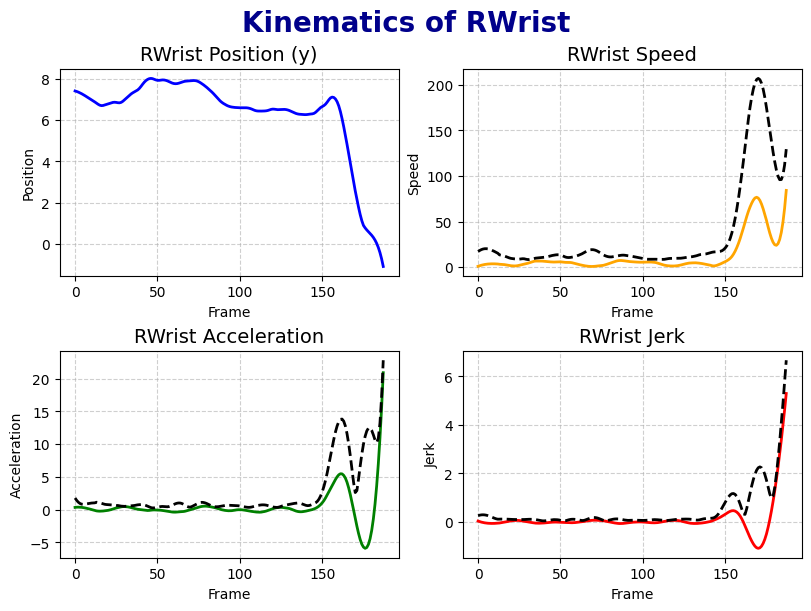
\includegraphics{03_TS_processing/01_TS_processing_motion_final_files/figure-pdf/cell-10-output-1.pdf}

\bookmarksetup{startatroot}

\chapter{Motion processing - inverse
kinematics}\label{motion-processing---inverse-kinematics}

In the previous notebook, we have extracted joint angles using OpenSim
((\textbf{ADDREF?})). Now again, we clean the data, smooth them, and
extract further information before saving it into csv file per trial

We can once again check what would be the proper filter

\begin{Shaded}
\begin{Highlighting}[]
\CommentTok{\# get all mot files in the folder}
\NormalTok{mot\_files }\OperatorTok{=}\NormalTok{ glob.glob(MTfolder }\OperatorTok{+} \StringTok{\textquotesingle{}*/P*/*/*.mot\textquotesingle{}}\NormalTok{, recursive}\OperatorTok{=}\VariableTok{True}\NormalTok{)}
\NormalTok{keypoints }\OperatorTok{=}\NormalTok{ [}\StringTok{\textquotesingle{}wrist\textquotesingle{}}\NormalTok{, }\StringTok{\textquotesingle{}pro\_sup\textquotesingle{}}\NormalTok{, }\StringTok{\textquotesingle{}elbow\textquotesingle{}}\NormalTok{, }\StringTok{\textquotesingle{}arm\textquotesingle{}}\NormalTok{, }\StringTok{\textquotesingle{}neck\textquotesingle{}}\NormalTok{, }\StringTok{\textquotesingle{}subtalar\textquotesingle{}}\NormalTok{, }\StringTok{\textquotesingle{}ankle\textquotesingle{}}\NormalTok{, }\StringTok{\textquotesingle{}knee\textquotesingle{}}\NormalTok{, }\StringTok{\textquotesingle{}hip\textquotesingle{}}\NormalTok{, }\StringTok{\textquotesingle{}pelvis\textquotesingle{}}\NormalTok{, }\StringTok{\textquotesingle{}L5\_S1\textquotesingle{}}\NormalTok{, }\StringTok{\textquotesingle{}L4\_L5\textquotesingle{}}\NormalTok{, }\StringTok{\textquotesingle{}L3\_L4\textquotesingle{}}\NormalTok{, }\StringTok{\textquotesingle{}L2\_L3\textquotesingle{}}\NormalTok{, }\StringTok{\textquotesingle{}L1\_L2\textquotesingle{}}\NormalTok{, }\StringTok{\textquotesingle{}L1\_T12\textquotesingle{}}\NormalTok{]}
\end{Highlighting}
\end{Shaded}

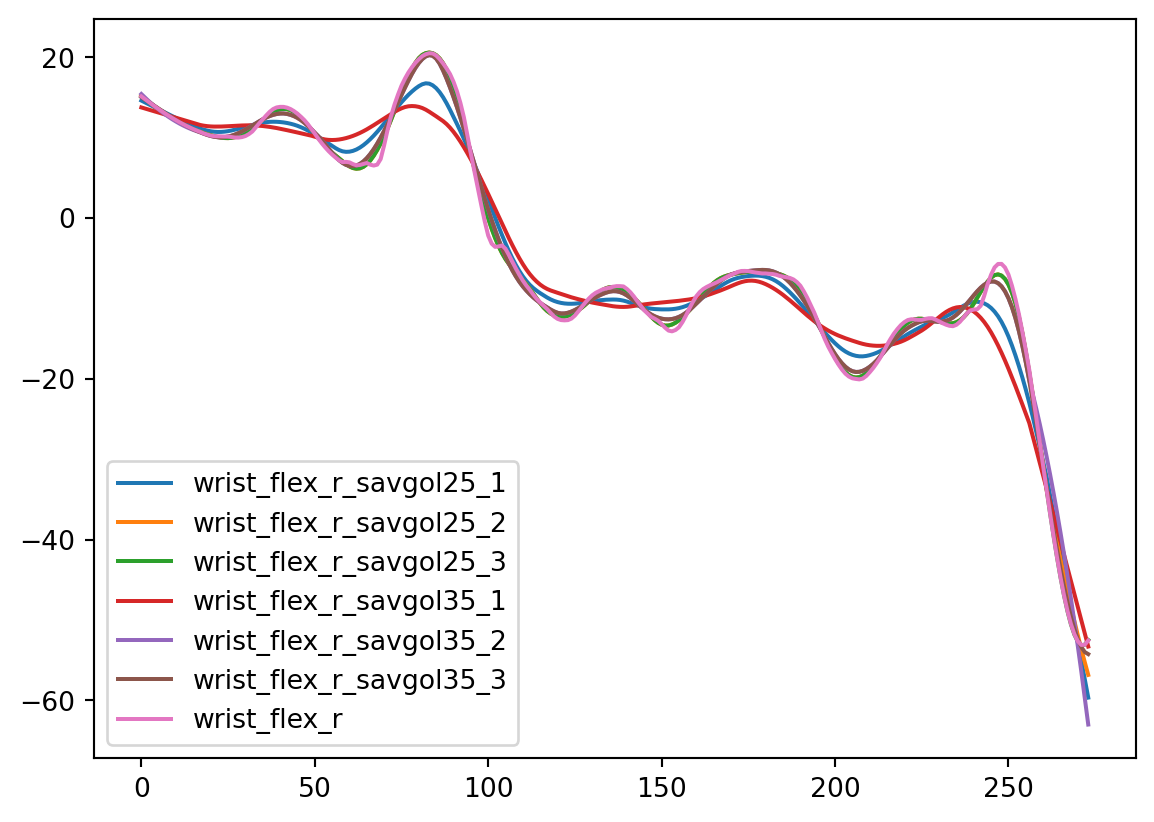
\includegraphics{03_TS_processing/01_TS_processing_motion_final_files/figure-pdf/cell-12-output-1.pdf}

And for legs

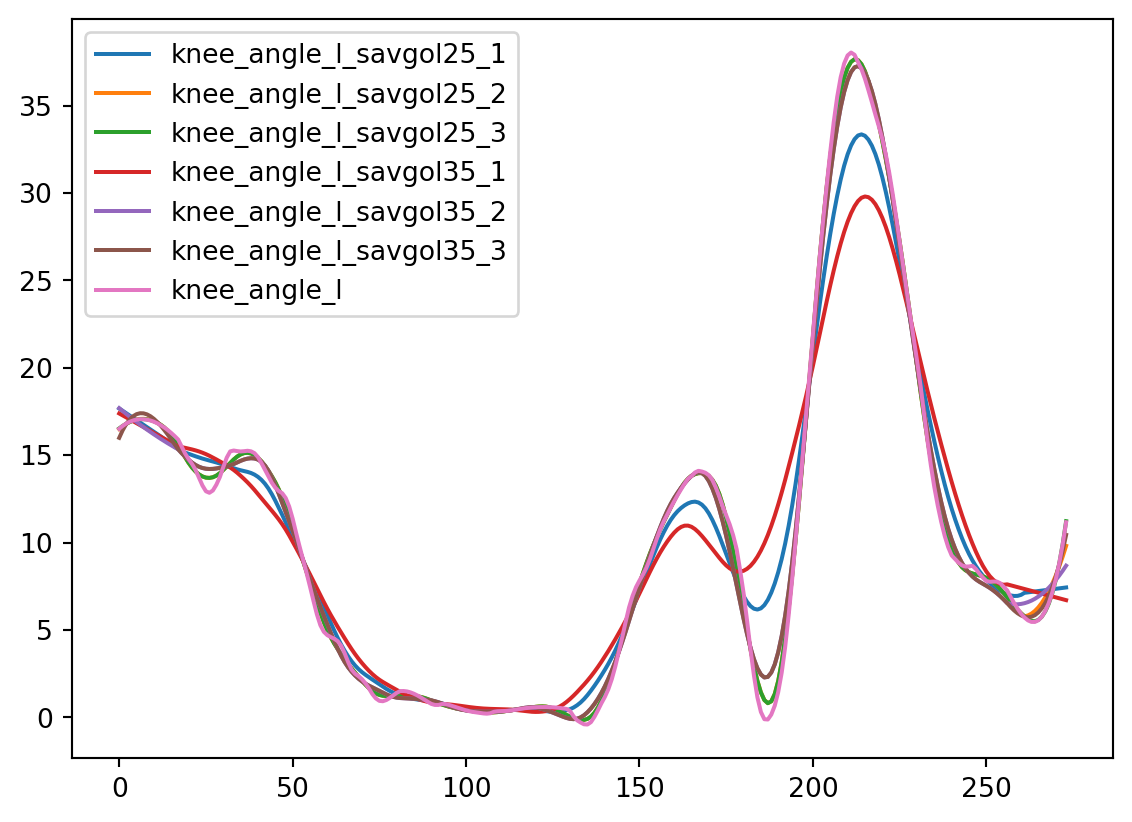
\includegraphics{03_TS_processing/01_TS_processing_motion_final_files/figure-pdf/cell-13-output-1.pdf}

We will apply a bit stronger filter of 1st order with span of 560 ms
because the data are more noisy than the kinematics.

\begin{Shaded}
\begin{Highlighting}[]
\CommentTok{\# get all mot files in the folder}
\NormalTok{mot\_files }\OperatorTok{=}\NormalTok{ glob.glob(MTfolder }\OperatorTok{+} \StringTok{\textquotesingle{}*/P*/*/*.mot\textquotesingle{}}\NormalTok{, recursive}\OperatorTok{=}\VariableTok{True}\NormalTok{)}
\NormalTok{keypoints }\OperatorTok{=}\NormalTok{ [}\StringTok{\textquotesingle{}wrist\textquotesingle{}}\NormalTok{, }\StringTok{\textquotesingle{}pro\_sup\textquotesingle{}}\NormalTok{, }\StringTok{\textquotesingle{}elbow\textquotesingle{}}\NormalTok{, }\StringTok{\textquotesingle{}arm\textquotesingle{}}\NormalTok{, }\StringTok{\textquotesingle{}neck\textquotesingle{}}\NormalTok{, }\StringTok{\textquotesingle{}subtalar\textquotesingle{}}\NormalTok{, }\StringTok{\textquotesingle{}ankle\textquotesingle{}}\NormalTok{, }\StringTok{\textquotesingle{}knee\textquotesingle{}}\NormalTok{, }\StringTok{\textquotesingle{}hip\textquotesingle{}}\NormalTok{, }\StringTok{\textquotesingle{}pelvis\textquotesingle{}}\NormalTok{, }\StringTok{\textquotesingle{}L5\_S1\textquotesingle{}}\NormalTok{, }\StringTok{\textquotesingle{}L4\_L5\textquotesingle{}}\NormalTok{, }\StringTok{\textquotesingle{}L3\_L4\textquotesingle{}}\NormalTok{, }\StringTok{\textquotesingle{}L2\_L3\textquotesingle{}}\NormalTok{, }\StringTok{\textquotesingle{}L1\_L2\textquotesingle{}}\NormalTok{, }\StringTok{\textquotesingle{}L1\_T12\textquotesingle{}}\NormalTok{]}

\ControlFlowTok{for}\NormalTok{ mot }\KeywordTok{in}\NormalTok{ mot\_files:}
    \CommentTok{\# get trialid}
\NormalTok{    trialid }\OperatorTok{=}\NormalTok{ mot.split(}\StringTok{\textquotesingle{}}\CharTok{\textbackslash{}\textbackslash{}}\StringTok{\textquotesingle{}}\NormalTok{)[}\OperatorTok{{-}}\DecValTok{1}\NormalTok{].split(}\StringTok{\textquotesingle{}.\textquotesingle{}}\NormalTok{)[}\DecValTok{0}\NormalTok{]}
    \BuiltInTok{print}\NormalTok{(}\StringTok{\textquotesingle{}working on \textquotesingle{}} \OperatorTok{+}\NormalTok{ trialid)}

    \CommentTok{\# get rid of the first element before \_}
\NormalTok{    trialid }\OperatorTok{=} \StringTok{\textquotesingle{}\_\textquotesingle{}}\NormalTok{.join(trialid.split(}\StringTok{\textquotesingle{}\_\textquotesingle{}}\NormalTok{)[}\DecValTok{1}\NormalTok{:])}

    \CommentTok{\# load it}
\NormalTok{    mot\_df }\OperatorTok{=}\NormalTok{ pd.read\_csv(mot, sep}\OperatorTok{=}\StringTok{\textquotesingle{}}\CharTok{\textbackslash{}t}\StringTok{\textquotesingle{}}\NormalTok{, skiprows}\OperatorTok{=}\DecValTok{10}\NormalTok{)}
    
    \CommentTok{\# pad 0 ms row}
\NormalTok{    padrow }\OperatorTok{=}\NormalTok{ mot\_df.iloc[}\DecValTok{0}\NormalTok{].copy()}
\NormalTok{    padrow[}\StringTok{\textquotesingle{}time\textquotesingle{}}\NormalTok{] }\OperatorTok{=} \DecValTok{0}

    \CommentTok{\# concatenate it to the beginning of mot\_df}
\NormalTok{    mot\_df }\OperatorTok{=}\NormalTok{ pd.concat([pd.DataFrame(padrow).T, mot\_df], ignore\_index}\OperatorTok{=}\VariableTok{True}\NormalTok{)}
    
    \CommentTok{\# get the sr}
\NormalTok{    sr }\OperatorTok{=} \DecValTok{1}\OperatorTok{/}\NormalTok{np.mean(np.diff(mot\_df[}\StringTok{\textquotesingle{}time\textquotesingle{}}\NormalTok{]))}

    \CommentTok{\#\#\#\#\# SMOOTHING \#\#\#\#\#\#}

    \CommentTok{\# smooth all columns except the firts time (time) and last (trialid)}
\NormalTok{    colstosmooth }\OperatorTok{=}\NormalTok{ [x }\ControlFlowTok{for}\NormalTok{ x }\KeywordTok{in}\NormalTok{ mot\_df.columns }\ControlFlowTok{if} \StringTok{\textquotesingle{}time\textquotesingle{}} \KeywordTok{not} \KeywordTok{in}\NormalTok{ x]}

    \CommentTok{\# smooth}
    \ControlFlowTok{for}\NormalTok{ col }\KeywordTok{in}\NormalTok{ colstosmooth:}
\NormalTok{        mot\_df[col] }\OperatorTok{=}\NormalTok{ scipy.signal.savgol\_filter(mot\_df[col], }\DecValTok{35}\NormalTok{, }\DecValTok{1}\NormalTok{)}
        \CommentTok{\# convert to radians}
\NormalTok{        mot\_df[col] }\OperatorTok{=}\NormalTok{ np.deg2rad(mot\_df[col])}

    \CommentTok{\# keep only columns you might use}
\NormalTok{    coi }\OperatorTok{=}\NormalTok{ [x }\ControlFlowTok{for}\NormalTok{ x }\KeywordTok{in}\NormalTok{ mot\_df.columns }\ControlFlowTok{if} \BuiltInTok{any}\NormalTok{(y }\KeywordTok{in}\NormalTok{ x }\ControlFlowTok{for}\NormalTok{ y }\KeywordTok{in}\NormalTok{ keypoints) }\KeywordTok{or} \StringTok{\textquotesingle{}time\textquotesingle{}} \KeywordTok{in}\NormalTok{ x }\KeywordTok{or} \StringTok{\textquotesingle{}TrialID\textquotesingle{}} \KeywordTok{in}\NormalTok{ x]}
\NormalTok{    mot\_df2 }\OperatorTok{=}\NormalTok{ mot\_df[coi]}

    \CommentTok{\#\#\#\#\# DERIVATIVES \#\#\#\#\#\#}

    \CommentTok{\# get derivatives}
\NormalTok{    mot\_df2 }\OperatorTok{=}\NormalTok{ get\_derivatives(mot\_df2, sr, [], [], }\StringTok{\textquotesingle{}angles\textquotesingle{}}\NormalTok{)}

    \CommentTok{\#\#\#\# AGGREGATING \#\#\#\#\#}

    \CommentTok{\# aggregate data}
\NormalTok{    mot\_df2 }\OperatorTok{=}\NormalTok{ aggregate\_keypoints(mot\_df2, }\StringTok{\textquotesingle{}speed\textquotesingle{}}\NormalTok{, }\StringTok{\textquotesingle{}\_angSpeed\_sum\textquotesingle{}}\NormalTok{, }\StringTok{\textquotesingle{}angles\textquotesingle{}}\NormalTok{)}
\NormalTok{    mot\_df2 }\OperatorTok{=}\NormalTok{ aggregate\_keypoints(mot\_df2, }\StringTok{\textquotesingle{}acc\textquotesingle{}}\NormalTok{, }\StringTok{\textquotesingle{}\_angAcc\_sum\textquotesingle{}}\NormalTok{, }\StringTok{\textquotesingle{}angles\textquotesingle{}}\NormalTok{)}
\NormalTok{    mot\_df2 }\OperatorTok{=}\NormalTok{ aggregate\_keypoints(mot\_df2, }\StringTok{\textquotesingle{}jerk\textquotesingle{}}\NormalTok{, }\StringTok{\textquotesingle{}\_angJerk\_sum\textquotesingle{}}\NormalTok{, }\StringTok{\textquotesingle{}angles\textquotesingle{}}\NormalTok{)}

    \CommentTok{\# add time and trialid}
\NormalTok{    mot\_df2[}\StringTok{\textquotesingle{}time\textquotesingle{}}\NormalTok{] }\OperatorTok{=}\NormalTok{ mot\_df[}\StringTok{\textquotesingle{}time\textquotesingle{}}\NormalTok{]}
    \CommentTok{\# convert time to ms}
\NormalTok{    mot\_df2[}\StringTok{\textquotesingle{}time\textquotesingle{}}\NormalTok{] }\OperatorTok{=}\NormalTok{ mot\_df2[}\StringTok{\textquotesingle{}time\textquotesingle{}}\NormalTok{]}\OperatorTok{*}\DecValTok{1000}
\NormalTok{    mot\_df2[}\StringTok{\textquotesingle{}TrialID\textquotesingle{}}\NormalTok{] }\OperatorTok{=}\NormalTok{ trialid}

    \CommentTok{\# write to csv}
\NormalTok{    mot\_df2.to\_csv(MTfolder\_processed }\OperatorTok{+} \StringTok{\textquotesingle{}/ik\_\textquotesingle{}} \OperatorTok{+}\NormalTok{ trialid }\OperatorTok{+} \StringTok{\textquotesingle{}.csv\textquotesingle{}}\NormalTok{, index}\OperatorTok{=}\VariableTok{False}\NormalTok{)}
\end{Highlighting}
\end{Shaded}

Here is an example file

\begin{longtable}[]{@{}llllllllllllllllllllll@{}}
\toprule\noalign{}
& time & pelvis\_tilt & pelvis\_list & pelvis\_rotation & pelvis\_tx &
pelvis\_ty & pelvis\_tz & hip\_flexion\_r & hip\_adduction\_r &
hip\_rotation\_r & ... & arm\_angAcc\_sum & pelvis\_angAcc\_sum &
spine\_angAcc\_sum & lowerbody\_angJerk\_sum & leg\_angJerk\_sum &
head\_angJerk\_sum & arm\_angJerk\_sum & pelvis\_angJerk\_sum &
spine\_angJerk\_sum & TrialID \\
\midrule\noalign{}
\endhead
\bottomrule\noalign{}
\endlastfoot
0 & 0.000 & -0.385372 & 1.436292 & -1.134475 & 0.004179 & 0.003296 &
0.002320 & 0.030322 & 0.066334 & -0.120157 & ... & 0.018420 & 0.005910 &
0.000564 & 0.001677 & 0.001134 & 0.000072 & 0.002143 & 0.001508 &
0.000201 & 0\_2\_31\_p1 \\
1 & 16.667 & -0.390499 & 1.435656 & -1.126051 & 0.004184 & 0.003296 &
0.002320 & 0.027478 & 0.068507 & -0.116957 & ... & 0.017830 & 0.006986 &
0.000388 & 0.001625 & 0.001109 & 0.000080 & 0.002075 & 0.001459 &
0.000197 & 0\_2\_31\_p1 \\
2 & 33.333 & -0.395626 & 1.435020 & -1.117626 & 0.004188 & 0.003296 &
0.002320 & 0.024634 & 0.070681 & -0.113757 & ... & 0.017425 & 0.008102 &
0.000226 & 0.001573 & 0.001084 & 0.000087 & 0.002013 & 0.001409 &
0.000193 & 0\_2\_31\_p1 \\
3 & 50.000 & -0.400753 & 1.434384 & -1.109202 & 0.004193 & 0.003296 &
0.002320 & 0.021791 & 0.072854 & -0.110557 & ... & 0.017219 & 0.009243 &
0.000146 & 0.001521 & 0.001059 & 0.000096 & 0.001956 & 0.001359 &
0.000189 & 0\_2\_31\_p1 \\
4 & 66.667 & -0.405879 & 1.433748 & -1.100778 & 0.004198 & 0.003296 &
0.002320 & 0.018947 & 0.075028 & -0.107356 & ... & 0.017218 & 0.010401 &
0.000247 & 0.001469 & 0.001034 & 0.000105 & 0.001904 & 0.001310 &
0.000185 & 0\_2\_31\_p1 \\
5 & 83.333 & -0.411006 & 1.433112 & -1.092354 & 0.004203 & 0.003296 &
0.002320 & 0.016103 & 0.077202 & -0.104156 & ... & 0.017423 & 0.011571 &
0.000412 & 0.001417 & 0.001009 & 0.000114 & 0.001859 & 0.001260 &
0.000181 & 0\_2\_31\_p1 \\
6 & 100.000 & -0.416133 & 1.432476 & -1.083929 & 0.004208 & 0.003296 &
0.002320 & 0.013260 & 0.079375 & -0.100956 & ... & 0.017827 & 0.012749 &
0.000590 & 0.001365 & 0.000984 & 0.000123 & 0.001821 & 0.001211 &
0.000177 & 0\_2\_31\_p1 \\
7 & 116.667 & -0.421260 & 1.431840 & -1.075505 & 0.004212 & 0.003296 &
0.002321 & 0.010416 & 0.081549 & -0.097756 & ... & 0.018416 & 0.013934 &
0.000772 & 0.001314 & 0.000959 & 0.000132 & 0.001789 & 0.001162 &
0.000174 & 0\_2\_31\_p1 \\
8 & 133.333 & -0.426386 & 1.431203 & -1.067081 & 0.004217 & 0.003296 &
0.002321 & 0.007572 & 0.083722 & -0.094555 & ... & 0.019174 & 0.015123 &
0.000955 & 0.001262 & 0.000935 & 0.000142 & 0.001766 & 0.001112 &
0.000170 & 0\_2\_31\_p1 \\
9 & 150.000 & -0.431513 & 1.430567 & -1.058656 & 0.004222 & 0.003296 &
0.002321 & 0.004729 & 0.085896 & -0.091355 & ... & 0.020081 & 0.016317 &
0.001140 & 0.001211 & 0.000910 & 0.000151 & 0.001750 & 0.001063 &
0.000166 & 0\_2\_31\_p1 \\
10 & 166.667 & -0.436640 & 1.429931 & -1.050232 & 0.004227 & 0.003296 &
0.002321 & 0.001885 & 0.088069 & -0.088155 & ... & 0.021118 & 0.017513 &
0.001325 & 0.001160 & 0.000886 & 0.000161 & 0.001742 & 0.001014 &
0.000162 & 0\_2\_31\_p1 \\
11 & 183.333 & -0.441767 & 1.429295 & -1.041808 & 0.004231 & 0.003296 &
0.002321 & -0.000959 & 0.090243 & -0.084955 & ... & 0.022267 & 0.018712
& 0.001510 & 0.001109 & 0.000862 & 0.000171 & 0.001743 & 0.000965 &
0.000159 & 0\_2\_31\_p1 \\
12 & 200.000 & -0.446893 & 1.428659 & -1.033384 & 0.004236 & 0.003296 &
0.002321 & -0.003802 & 0.092416 & -0.081755 & ... & 0.023512 & 0.019913
& 0.001695 & 0.001059 & 0.000837 & 0.000181 & 0.001752 & 0.000916 &
0.000155 & 0\_2\_31\_p1 \\
13 & 216.667 & -0.452020 & 1.428023 & -1.024959 & 0.004241 & 0.003296 &
0.002321 & -0.006646 & 0.094590 & -0.078554 & ... & 0.024838 & 0.021116
& 0.001881 & 0.001008 & 0.000814 & 0.000191 & 0.001768 & 0.000867 &
0.000152 & 0\_2\_31\_p1 \\
14 & 233.333 & -0.457147 & 1.427387 & -1.016535 & 0.004246 & 0.003296 &
0.002321 & -0.009489 & 0.096763 & -0.075354 & ... & 0.026232 & 0.022319
& 0.002066 & 0.000958 & 0.000790 & 0.000201 & 0.001793 & 0.000818 &
0.000148 & 0\_2\_31\_p1 \\
\end{longtable}

Here we can see the joint angle speed next to kinematic speed.

\includegraphics{03_TS_processing/01_TS_processing_motion_final_files/figure-pdf/cell-16-output-1.pdf}

\bookmarksetup{startatroot}

\chapter{Motion processing - inverse
dynamics}\label{motion-processing---inverse-dynamics}

Now we do exactly the same also for inverse dynamics data (joint
torques).

\begin{Shaded}
\begin{Highlighting}[]
\CommentTok{\# in MTfolders, find all sto files}
\NormalTok{sto\_files }\OperatorTok{=}\NormalTok{ glob.glob(MTfolder }\OperatorTok{+} \StringTok{\textquotesingle{}*/P*/*/*.sto\textquotesingle{}}\NormalTok{, recursive}\OperatorTok{=}\VariableTok{True}\NormalTok{)}
\NormalTok{sto\_files }\OperatorTok{=}\NormalTok{ [x }\ControlFlowTok{for}\NormalTok{ x }\KeywordTok{in}\NormalTok{ sto\_files }\ControlFlowTok{if} \StringTok{\textquotesingle{}ID\textquotesingle{}} \KeywordTok{in}\NormalTok{ x]}
\end{Highlighting}
\end{Shaded}

Let's once again check the different smoothing strengths

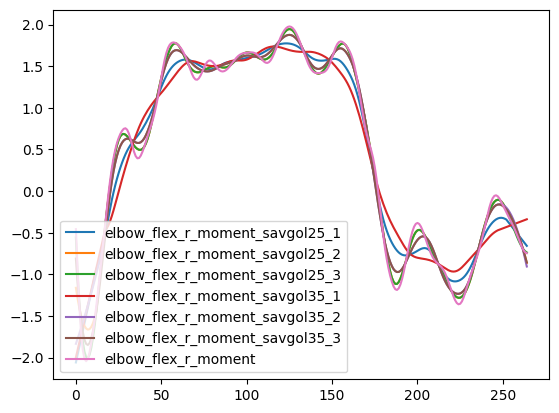
\includegraphics{03_TS_processing/01_TS_processing_motion_final_files/figure-pdf/cell-18-output-1.pdf}

And for legs

\includegraphics{03_TS_processing/01_TS_processing_motion_final_files/figure-pdf/cell-19-output-1.pdf}

We will again reuse 1st order Savitzky-Golay filter with window of 560
ms for the moments and their first derivate (moment change).

\begin{Shaded}
\begin{Highlighting}[]
\CommentTok{\# in MTfolders, find all sto files}
\NormalTok{sto\_files }\OperatorTok{=}\NormalTok{ glob.glob(MTfolder }\OperatorTok{+} \StringTok{\textquotesingle{}*/P*/*/*.sto\textquotesingle{}}\NormalTok{, recursive}\OperatorTok{=}\VariableTok{True}\NormalTok{)}
\NormalTok{sto\_files }\OperatorTok{=}\NormalTok{ [x }\ControlFlowTok{for}\NormalTok{ x }\KeywordTok{in}\NormalTok{ sto\_files }\ControlFlowTok{if} \StringTok{\textquotesingle{}ID\textquotesingle{}} \KeywordTok{in}\NormalTok{ x]}

\ControlFlowTok{for}\NormalTok{ sto }\KeywordTok{in}\NormalTok{ sto\_files:}

    \CommentTok{\# from the filename, get the trialid}
\NormalTok{    trialid }\OperatorTok{=}\NormalTok{ sto.split(}\StringTok{\textquotesingle{}}\CharTok{\textbackslash{}\textbackslash{}}\StringTok{\textquotesingle{}}\NormalTok{)[}\OperatorTok{{-}}\DecValTok{1}\NormalTok{].split(}\StringTok{\textquotesingle{}.\textquotesingle{}}\NormalTok{)[}\DecValTok{0}\NormalTok{]}
\NormalTok{    trialid }\OperatorTok{=} \StringTok{\textquotesingle{}\_\textquotesingle{}}\NormalTok{.join(trialid.split(}\StringTok{\textquotesingle{}\_\textquotesingle{}}\NormalTok{)[:}\OperatorTok{{-}}\DecValTok{1}\NormalTok{])}
\NormalTok{    trialid }\OperatorTok{=} \StringTok{\textquotesingle{}\_\textquotesingle{}}\NormalTok{.join(trialid.split(}\StringTok{\textquotesingle{}\_\textquotesingle{}}\NormalTok{)[}\DecValTok{1}\NormalTok{:])}

    \BuiltInTok{print}\NormalTok{(}\StringTok{\textquotesingle{}working on \textquotesingle{}} \OperatorTok{+}\NormalTok{ trialid)}

    \CommentTok{\# load it}
\NormalTok{    id\_df }\OperatorTok{=}\NormalTok{ pd.read\_csv(sto, sep}\OperatorTok{=}\StringTok{\textquotesingle{}}\CharTok{\textbackslash{}t}\StringTok{\textquotesingle{}}\NormalTok{, skiprows}\OperatorTok{=}\DecValTok{6}\NormalTok{)}

    \CommentTok{\# pad 0 ms row}
\NormalTok{    padrow }\OperatorTok{=}\NormalTok{ id\_df.iloc[}\DecValTok{0}\NormalTok{].copy()}
\NormalTok{    padrow[}\StringTok{\textquotesingle{}time\textquotesingle{}}\NormalTok{] }\OperatorTok{=} \DecValTok{0}

    \CommentTok{\# concatenate it to the beginning of id\_df}
\NormalTok{    id\_df }\OperatorTok{=}\NormalTok{ pd.concat([pd.DataFrame(padrow).T, id\_df], ignore\_index}\OperatorTok{=}\VariableTok{True}\NormalTok{)}

    \CommentTok{\#\#\#\#\# SMOOTHING \#\#\#\#\#}

    \CommentTok{\# smooth all columns except the firts time (time) and last (trialid)}
\NormalTok{    colstosmooth }\OperatorTok{=}\NormalTok{ [x }\ControlFlowTok{for}\NormalTok{ x }\KeywordTok{in}\NormalTok{ id\_df.columns }\ControlFlowTok{if} \StringTok{\textquotesingle{}time\textquotesingle{}} \KeywordTok{not} \KeywordTok{in}\NormalTok{ x]}
\NormalTok{    colstosmooth }\OperatorTok{=}\NormalTok{ [x }\ControlFlowTok{for}\NormalTok{ x }\KeywordTok{in}\NormalTok{ colstosmooth }\ControlFlowTok{if} \StringTok{\textquotesingle{}TrialID\textquotesingle{}} \KeywordTok{not} \KeywordTok{in}\NormalTok{ x]}

    \CommentTok{\# smooth}
    \ControlFlowTok{for}\NormalTok{ col }\KeywordTok{in}\NormalTok{ colstosmooth:}
\NormalTok{        id\_df[col] }\OperatorTok{=}\NormalTok{ scipy.signal.savgol\_filter(id\_df[col], }\DecValTok{35}\NormalTok{, }\DecValTok{1}\NormalTok{)}

    \CommentTok{\#\#\#\#\# AGGREGATING \#\#\#\#\#}

    \CommentTok{\# get aggregated euclidian sum for each joint group}
\NormalTok{    id\_df }\OperatorTok{=}\NormalTok{ aggregate\_keypoints(id\_df, }\StringTok{\textquotesingle{}moment\textquotesingle{}}\NormalTok{, }\StringTok{\textquotesingle{}\_moment\_sum\textquotesingle{}}\NormalTok{, }\StringTok{\textquotesingle{}angles\textquotesingle{}}\NormalTok{)}

    \CommentTok{\#\#\#\# TORQUE CHANGE \#\#\#\#\#}

    \CommentTok{\# for each moment col, we will also calculate the change }
\NormalTok{    torquestodiff }\OperatorTok{=}\NormalTok{ [x }\ControlFlowTok{for}\NormalTok{ x }\KeywordTok{in}\NormalTok{ id\_df.columns }\ControlFlowTok{if} \StringTok{\textquotesingle{}moment\textquotesingle{}} \KeywordTok{in}\NormalTok{ x]}

    \ControlFlowTok{for}\NormalTok{ col }\KeywordTok{in}\NormalTok{ torquestodiff:}
\NormalTok{        torquechange }\OperatorTok{=}\NormalTok{ np.}\BuiltInTok{abs}\NormalTok{(np.insert(np.diff(id\_df[col]), }\DecValTok{0}\NormalTok{, }\DecValTok{0}\NormalTok{))}
\NormalTok{        torquechange\_smoothed }\OperatorTok{=}\NormalTok{ scipy.signal.savgol\_filter(torquechange, }\DecValTok{35}\NormalTok{, }\DecValTok{1}\NormalTok{)}
        \CommentTok{\# new data}
\NormalTok{        new\_data }\OperatorTok{=}\NormalTok{ pd.DataFrame(\{col }\OperatorTok{+} \StringTok{\textquotesingle{}\_change\textquotesingle{}}\NormalTok{: torquechange\_smoothed\})}
\NormalTok{        id\_df }\OperatorTok{=}\NormalTok{ pd.concat([id\_df, new\_data], axis}\OperatorTok{=}\DecValTok{1}\NormalTok{)}
    
    \CommentTok{\# convert time to ms}
\NormalTok{    id\_df[}\StringTok{\textquotesingle{}time\textquotesingle{}}\NormalTok{] }\OperatorTok{=}\NormalTok{ id\_df[}\StringTok{\textquotesingle{}time\textquotesingle{}}\NormalTok{]}\OperatorTok{*}\DecValTok{1000}
        \CommentTok{\# add trialid}
\NormalTok{    id\_df[}\StringTok{\textquotesingle{}TrialID\textquotesingle{}}\NormalTok{] }\OperatorTok{=}\NormalTok{ trialid}

    \CommentTok{\# write to csv}
\NormalTok{    id\_df.to\_csv(MTfolder\_processed }\OperatorTok{+} \StringTok{\textquotesingle{}/id\_\textquotesingle{}} \OperatorTok{+}\NormalTok{ trialid }\OperatorTok{+} \StringTok{\textquotesingle{}.csv\textquotesingle{}}\NormalTok{, index}\OperatorTok{=}\VariableTok{False}\NormalTok{)}
\end{Highlighting}
\end{Shaded}

Here is an example file

\begin{longtable}[]{@{}llllllllllllllllllllll@{}}
\toprule\noalign{}
& time & pelvis\_tilt\_moment & pelvis\_list\_moment &
pelvis\_rotation\_moment & pelvis\_tx\_force & pelvis\_ty\_force &
pelvis\_tz\_force & hip\_flexion\_r\_moment & hip\_adduction\_r\_moment
& hip\_rotation\_r\_moment & ... & wrist\_dev\_r\_moment\_change &
wrist\_flex\_l\_moment\_change & wrist\_dev\_l\_moment\_change &
lowerbody\_moment\_sum\_change & leg\_moment\_sum\_change &
head\_moment\_sum\_change & arm\_moment\_sum\_change &
pelvis\_moment\_sum\_change & spine\_moment\_sum\_change & TrialID \\
\midrule\noalign{}
\endhead
\bottomrule\noalign{}
\endlastfoot
0 & 0.000 & 5.708250 & 110.055801 & 3.561396 & 24.712276 & 586.204253 &
23.558725 & -55.382619 & 11.617392 & 0.481999 & ... & -0.000634 &
0.001559 & 0.006968 & 4.270216 & 0.082287 & 0.173882 & 0.060730 &
5.849430 & -0.071949 & 0\_2\_6\_p0 \\
1 & 16.561 & 5.445360 & 104.296342 & 3.540215 & 23.583740 & 588.019295 &
22.469841 & -55.005510 & 11.400441 & 0.459807 & ... & -0.000500 &
0.001563 & 0.006837 & 4.154601 & 0.087671 & 0.171330 & 0.059875 &
5.757471 & -0.046640 & 0\_2\_6\_p0 \\
2 & 33.227 & 5.182469 & 98.536882 & 3.519034 & 22.455203 & 589.834337 &
21.380958 & -54.628401 & 11.183491 & 0.437616 & ... & -0.000367 &
0.001566 & 0.006707 & 4.038986 & 0.093056 & 0.168779 & 0.059020 &
5.665511 & -0.021331 & 0\_2\_6\_p0 \\
3 & 49.893 & 4.919578 & 92.777423 & 3.497852 & 21.326667 & 591.649378 &
20.292074 & -54.251292 & 10.966541 & 0.415425 & ... & -0.000233 &
0.001569 & 0.006577 & 3.923371 & 0.098441 & 0.166227 & 0.058165 &
5.573551 & 0.003978 & 0\_2\_6\_p0 \\
4 & 66.559 & 4.656687 & 87.017963 & 3.476671 & 20.198130 & 593.464420 &
19.203191 & -53.874183 & 10.749590 & 0.393234 & ... & -0.000099 &
0.001572 & 0.006446 & 3.807756 & 0.103826 & 0.163675 & 0.057311 &
5.481591 & 0.029287 & 0\_2\_6\_p0 \\
5 & 83.225 & 4.393797 & 81.258504 & 3.455490 & 19.069594 & 595.279462 &
18.114307 & -53.497074 & 10.532640 & 0.371042 & ... & 0.000034 &
0.001575 & 0.006316 & 3.692141 & 0.109210 & 0.161124 & 0.056456 &
5.389631 & 0.054596 & 0\_2\_6\_p0 \\
6 & 99.891 & 4.130906 & 75.499045 & 3.434309 & 17.941057 & 597.094504 &
17.025423 & -53.119965 & 10.315690 & 0.348851 & ... & 0.000168 &
0.001579 & 0.006185 & 3.576526 & 0.114595 & 0.158572 & 0.055601 &
5.297671 & 0.079905 & 0\_2\_6\_p0 \\
7 & 116.557 & 3.868015 & 69.739585 & 3.413128 & 16.812521 & 598.909545 &
15.936540 & -52.742856 & 10.098739 & 0.326660 & ... & 0.000302 &
0.001582 & 0.006055 & 3.460911 & 0.119980 & 0.156020 & 0.054746 &
5.205711 & 0.105214 & 0\_2\_6\_p0 \\
8 & 133.223 & 3.605125 & 63.980126 & 3.391947 & 15.683985 & 600.724587 &
14.847656 & -52.365747 & 9.881789 & 0.304468 & ... & 0.000435 & 0.001585
& 0.005924 & 3.345295 & 0.125364 & 0.153469 & 0.053891 & 5.113751 &
0.130523 & 0\_2\_6\_p0 \\
9 & 149.889 & 3.342234 & 58.220667 & 3.370766 & 14.555448 & 602.539629 &
13.758773 & -51.988638 & 9.664839 & 0.282277 & ... & 0.000569 & 0.001588
& 0.005794 & 3.229680 & 0.130749 & 0.150917 & 0.053037 & 5.021791 &
0.155832 & 0\_2\_6\_p0 \\
10 & 166.555 & 3.079343 & 52.461207 & 3.349585 & 13.426912 & 604.354671
& 12.669889 & -51.611529 & 9.447888 & 0.260086 & ... & 0.000703 &
0.001591 & 0.005664 & 3.114065 & 0.136134 & 0.148366 & 0.052182 &
4.929831 & 0.181140 & 0\_2\_6\_p0 \\
11 & 183.221 & 2.816452 & 46.701748 & 3.328404 & 12.298375 & 606.169712
& 11.581005 & -51.234420 & 9.230938 & 0.237895 & ... & 0.000837 &
0.001595 & 0.005533 & 2.998450 & 0.141519 & 0.145814 & 0.051327 &
4.837872 & 0.206449 & 0\_2\_6\_p0 \\
12 & 199.887 & 2.553562 & 40.942289 & 3.307223 & 11.169839 & 607.984754
& 10.492122 & -50.857311 & 9.013988 & 0.215703 & ... & 0.000970 &
0.001598 & 0.005403 & 2.882835 & 0.146903 & 0.143262 & 0.050472 &
4.745912 & 0.231758 & 0\_2\_6\_p0 \\
13 & 216.553 & 2.290671 & 35.182829 & 3.286042 & 10.041302 & 609.799796
& 9.403238 & -50.480202 & 8.797038 & 0.193512 & ... & 0.001104 &
0.001601 & 0.005272 & 2.767220 & 0.152288 & 0.140711 & 0.049618 &
4.653952 & 0.257067 & 0\_2\_6\_p0 \\
14 & 233.219 & 2.027780 & 29.423370 & 3.264861 & 8.912766 & 611.614838 &
8.314355 & -50.103093 & 8.580087 & 0.171321 & ... & 0.001238 & 0.001604
& 0.005142 & 2.651605 & 0.157673 & 0.138159 & 0.048763 & 4.561992 &
0.282376 & 0\_2\_6\_p0 \\
\end{longtable}

Now we can check by ploting the joint moment change against kinematic
acceleration

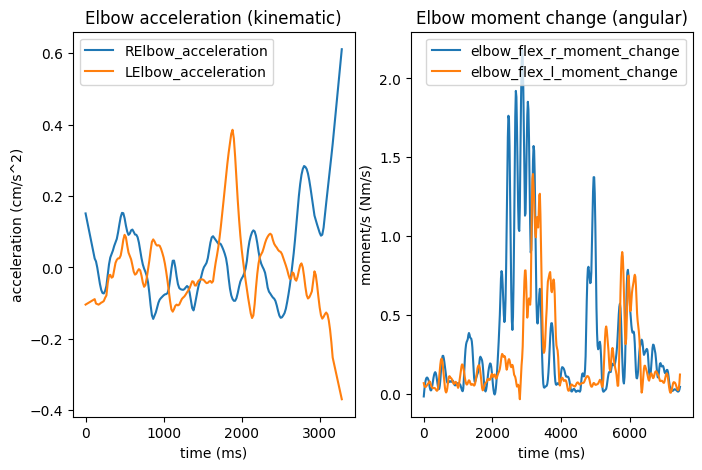
\includegraphics{03_TS_processing/01_TS_processing_motion_final_files/figure-pdf/cell-22-output-1.pdf}

\bookmarksetup{startatroot}

\chapter{Balance Board (Ground reaction forces) -
processing}\label{balance-board-ground-reaction-forces---processing}

Lastly, we need to process the balance board data. We apply 5th order
Savitzky-Golay filter to windows of 102 ms. To have a measure for
postural adjustments, we compute the change in 2D magnitude (L2 norm of
the center of pressure x and y) in center of pressure.

\begin{Shaded}
\begin{Highlighting}[]
\NormalTok{BB\_files }\OperatorTok{=}\NormalTok{ glob.glob(BBfolder }\OperatorTok{+} \StringTok{\textquotesingle{}*BalanceBoard*.csv\textquotesingle{}}\NormalTok{, recursive}\OperatorTok{=}\VariableTok{True}\NormalTok{)}

\ControlFlowTok{for}\NormalTok{ bb }\KeywordTok{in}\NormalTok{ BB\_files:}
    \CommentTok{\# get trialid}
\NormalTok{    trialid }\OperatorTok{=}\NormalTok{ bb.split(}\StringTok{\textquotesingle{}}\CharTok{\textbackslash{}\textbackslash{}}\StringTok{\textquotesingle{}}\NormalTok{)[}\OperatorTok{{-}}\DecValTok{1}\NormalTok{].split(}\StringTok{\textquotesingle{}.\textquotesingle{}}\NormalTok{)[}\DecValTok{0}\NormalTok{]}
    \CommentTok{\# get the first, second, fourth, nineth elements}
\NormalTok{    trialid }\OperatorTok{=} \StringTok{\textquotesingle{}\_\textquotesingle{}}\NormalTok{.join(trialid.split(}\StringTok{\textquotesingle{}\_\textquotesingle{}}\NormalTok{)[:}\DecValTok{2}\NormalTok{] }\OperatorTok{+}\NormalTok{ trialid.split(}\StringTok{\textquotesingle{}\_\textquotesingle{}}\NormalTok{)[}\DecValTok{3}\NormalTok{:}\DecValTok{4}\NormalTok{] }\OperatorTok{+}\NormalTok{ trialid.split(}\StringTok{\textquotesingle{}\_\textquotesingle{}}\NormalTok{)[}\DecValTok{8}\NormalTok{:}\DecValTok{9}\NormalTok{])}

    \BuiltInTok{print}\NormalTok{(}\StringTok{\textquotesingle{}working on \textquotesingle{}} \OperatorTok{+}\NormalTok{ trialid)}

    \CommentTok{\# because we are going to merge on bb, we will store also more information}
\NormalTok{    fileinfo }\OperatorTok{=}\NormalTok{ bb.split(}\StringTok{\textquotesingle{}}\CharTok{\textbackslash{}\textbackslash{}}\StringTok{\textquotesingle{}}\NormalTok{)[}\OperatorTok{{-}}\DecValTok{1}\NormalTok{].split(}\StringTok{\textquotesingle{}.\textquotesingle{}}\NormalTok{)[}\DecValTok{0}\NormalTok{]}

    \CommentTok{\# if second element is 1, we will store last three elements}
    \ControlFlowTok{if}\NormalTok{ fileinfo.split(}\StringTok{\textquotesingle{}\_\textquotesingle{}}\NormalTok{)[}\DecValTok{1}\NormalTok{] }\OperatorTok{==} \StringTok{\textquotesingle{}1\textquotesingle{}}\NormalTok{:}
        \CommentTok{\# if there is not \textquotesingle{}corrected\textquotesingle{} in the name, we will store last three elements}
        \ControlFlowTok{if} \StringTok{\textquotesingle{}corrected\textquotesingle{}} \KeywordTok{not} \KeywordTok{in}\NormalTok{ fileinfo:}
\NormalTok{            info }\OperatorTok{=} \StringTok{\textquotesingle{}\_\textquotesingle{}}\NormalTok{.join(fileinfo.split(}\StringTok{\textquotesingle{}\_\textquotesingle{}}\NormalTok{)[}\OperatorTok{{-}}\DecValTok{3}\NormalTok{:])}
        \ControlFlowTok{else}\NormalTok{:}
\NormalTok{            info }\OperatorTok{=} \StringTok{\textquotesingle{}\_\textquotesingle{}}\NormalTok{.join(fileinfo.split(}\StringTok{\textquotesingle{}\_\textquotesingle{}}\NormalTok{)[}\OperatorTok{{-}}\DecValTok{4}\NormalTok{:])}
    \ControlFlowTok{elif}\NormalTok{ fileinfo.split(}\StringTok{\textquotesingle{}\_\textquotesingle{}}\NormalTok{)[}\DecValTok{1}\NormalTok{] }\OperatorTok{==} \StringTok{\textquotesingle{}2\textquotesingle{}}\NormalTok{:}
        \CommentTok{\# otherwise we store last four elements (5 when corrected)}
        \ControlFlowTok{if} \StringTok{\textquotesingle{}corrected\textquotesingle{}} \KeywordTok{not} \KeywordTok{in}\NormalTok{ fileinfo:}
\NormalTok{            info }\OperatorTok{=} \StringTok{\textquotesingle{}\_\textquotesingle{}}\NormalTok{.join(fileinfo.split(}\StringTok{\textquotesingle{}\_\textquotesingle{}}\NormalTok{)[}\OperatorTok{{-}}\DecValTok{4}\NormalTok{:])}
        \ControlFlowTok{else}\NormalTok{:}
\NormalTok{            info }\OperatorTok{=} \StringTok{\textquotesingle{}\_\textquotesingle{}}\NormalTok{.join(fileinfo.split(}\StringTok{\textquotesingle{}\_\textquotesingle{}}\NormalTok{)[}\OperatorTok{{-}}\DecValTok{5}\NormalTok{:])}

    \CommentTok{\# Load the balanceboard data}
\NormalTok{    df\_bb }\OperatorTok{=}\NormalTok{ pd.read\_csv(bb)}

    \CommentTok{\# Rename columns}
\NormalTok{    df\_bb.columns }\OperatorTok{=}\NormalTok{ [}\StringTok{\textquotesingle{}time\_s\textquotesingle{}}\NormalTok{, }\StringTok{\textquotesingle{}left\_back\textquotesingle{}}\NormalTok{, }\StringTok{\textquotesingle{}right\_forward\textquotesingle{}}\NormalTok{, }\StringTok{\textquotesingle{}right\_back\textquotesingle{}}\NormalTok{, }\StringTok{\textquotesingle{}left\_forward\textquotesingle{}}\NormalTok{]}

    \CommentTok{\# Calculate sampling rate}
\NormalTok{    bbsamp }\OperatorTok{=} \DecValTok{1} \OperatorTok{/}\NormalTok{ np.mean(np.diff(df\_bb[}\StringTok{\textquotesingle{}time\_s\textquotesingle{}}\NormalTok{] }\OperatorTok{{-}} \BuiltInTok{min}\NormalTok{(df\_bb[}\StringTok{\textquotesingle{}time\_s\textquotesingle{}}\NormalTok{])))}

    \CommentTok{\# Apply Savitzky{-}Golay filter to smooth the data}
    \ControlFlowTok{for}\NormalTok{ col }\KeywordTok{in}\NormalTok{ df\_bb.columns[}\DecValTok{1}\NormalTok{:]:}
\NormalTok{        df\_bb[col] }\OperatorTok{=}\NormalTok{ scipy.signal.savgol\_filter(df\_bb[col], }\DecValTok{51}\NormalTok{, }\DecValTok{5}\NormalTok{) }\CommentTok{\# window of 102 ms}

    \CommentTok{\# Calculate COPX and COPY}
\NormalTok{    COPX }\OperatorTok{=}\NormalTok{ (df\_bb[}\StringTok{\textquotesingle{}right\_forward\textquotesingle{}}\NormalTok{] }\OperatorTok{+}\NormalTok{ df\_bb[}\StringTok{\textquotesingle{}right\_back\textquotesingle{}}\NormalTok{]) }\OperatorTok{{-}}\NormalTok{ (df\_bb[}\StringTok{\textquotesingle{}left\_forward\textquotesingle{}}\NormalTok{] }\OperatorTok{+}\NormalTok{ df\_bb[}\StringTok{\textquotesingle{}left\_back\textquotesingle{}}\NormalTok{])}
\NormalTok{    COPY }\OperatorTok{=}\NormalTok{ (df\_bb[}\StringTok{\textquotesingle{}right\_forward\textquotesingle{}}\NormalTok{] }\OperatorTok{+}\NormalTok{ df\_bb[}\StringTok{\textquotesingle{}left\_forward\textquotesingle{}}\NormalTok{]) }\OperatorTok{{-}}\NormalTok{ (df\_bb[}\StringTok{\textquotesingle{}left\_back\textquotesingle{}}\NormalTok{] }\OperatorTok{+}\NormalTok{ df\_bb[}\StringTok{\textquotesingle{}right\_back\textquotesingle{}}\NormalTok{])}

    \CommentTok{\# Calculate COPXc and COPYc }
\NormalTok{    df\_bb[}\StringTok{\textquotesingle{}COPXc\textquotesingle{}}\NormalTok{] }\OperatorTok{=}\NormalTok{ scipy.signal.savgol\_filter(np.insert(np.diff(COPX), }\DecValTok{0}\NormalTok{, }\DecValTok{0}\NormalTok{), }\DecValTok{51}\NormalTok{, }\DecValTok{5}\NormalTok{) }
\NormalTok{    df\_bb[}\StringTok{\textquotesingle{}COPYc\textquotesingle{}}\NormalTok{] }\OperatorTok{=}\NormalTok{ scipy.signal.savgol\_filter(np.insert(np.diff(COPY), }\DecValTok{0}\NormalTok{, }\DecValTok{0}\NormalTok{), }\DecValTok{51}\NormalTok{, }\DecValTok{5}\NormalTok{)}

    \CommentTok{\# Calculate COPc}
\NormalTok{    df\_bb[}\StringTok{\textquotesingle{}COPc\textquotesingle{}}\NormalTok{] }\OperatorTok{=}\NormalTok{ np.sqrt(df\_bb[}\StringTok{\textquotesingle{}COPXc\textquotesingle{}}\NormalTok{]}\OperatorTok{**}\DecValTok{2} \OperatorTok{+}\NormalTok{ df\_bb[}\StringTok{\textquotesingle{}COPYc\textquotesingle{}}\NormalTok{]}\OperatorTok{**}\DecValTok{2}\NormalTok{)}

    \CommentTok{\# restart the time so that starts from 0}
\NormalTok{    df\_bb[}\StringTok{\textquotesingle{}time\_s\textquotesingle{}}\NormalTok{] }\OperatorTok{=}\NormalTok{ df\_bb[}\StringTok{\textquotesingle{}time\_s\textquotesingle{}}\NormalTok{] }\OperatorTok{{-}} \BuiltInTok{min}\NormalTok{(df\_bb[}\StringTok{\textquotesingle{}time\_s\textquotesingle{}}\NormalTok{])}
    \CommentTok{\# convert to ms}
\NormalTok{    df\_bb[}\StringTok{\textquotesingle{}time\_s\textquotesingle{}}\NormalTok{] }\OperatorTok{=}\NormalTok{ df\_bb[}\StringTok{\textquotesingle{}time\_s\textquotesingle{}}\NormalTok{]}\OperatorTok{*}\DecValTok{1000}

    \CommentTok{\# rename time\_s to time}
\NormalTok{    df\_bb.rename(columns}\OperatorTok{=}\NormalTok{\{}\StringTok{\textquotesingle{}time\_s\textquotesingle{}}\NormalTok{: }\StringTok{\textquotesingle{}time\textquotesingle{}}\NormalTok{\}, inplace}\OperatorTok{=}\VariableTok{True}\NormalTok{)}

    \CommentTok{\# Add trialid}
\NormalTok{    df\_bb[}\StringTok{\textquotesingle{}TrialID\textquotesingle{}}\NormalTok{] }\OperatorTok{=}\NormalTok{ trialid}
    \CommentTok{\# Add info}
\NormalTok{    df\_bb[}\StringTok{\textquotesingle{}FileInfo\textquotesingle{}}\NormalTok{] }\OperatorTok{=}\NormalTok{ info}

    \CommentTok{\# Write as csv to MTfolder\_processed}
\NormalTok{    df\_bb.to\_csv(MTfolder\_processed }\OperatorTok{+} \StringTok{\textquotesingle{}/bb\_\textquotesingle{}} \OperatorTok{+}\NormalTok{ trialid }\OperatorTok{+} \StringTok{\textquotesingle{}.csv\textquotesingle{}}\NormalTok{, index}\OperatorTok{=}\VariableTok{False}\NormalTok{)}
\end{Highlighting}
\end{Shaded}

Here is an example of a file

\begin{longtable}[]{@{}lllllllllll@{}}
\toprule\noalign{}
& time & left\_back & right\_forward & right\_back & left\_forward &
COPXc & COPYc & COPc & TrialID & FileInfo \\
\midrule\noalign{}
\endhead
\bottomrule\noalign{}
\endlastfoot
0 & 0.000000 & 1.110243 & 0.835766 & 1.506559 & 1.389595 & -0.000199 &
-0.000163 & 0.000257 & 0\_2\_96\_p1 & p1\_sneeuw\_geluiden\_c1 \\
1 & 2.000053 & 1.110623 & 0.835862 & 1.506878 & 1.389899 & -0.000154 &
-0.000212 & 0.000262 & 0\_2\_96\_p1 & p1\_sneeuw\_geluiden\_c1 \\
2 & 4.000105 & 1.110933 & 0.835914 & 1.507148 & 1.390102 & -0.000109 &
-0.000258 & 0.000280 & 0\_2\_96\_p1 & p1\_sneeuw\_geluiden\_c1 \\
3 & 6.000158 & 1.111185 & 0.835931 & 1.507381 & 1.390221 & -0.000067 &
-0.000299 & 0.000307 & 0\_2\_96\_p1 & p1\_sneeuw\_geluiden\_c1 \\
4 & 8.000211 & 1.111393 & 0.835922 & 1.507586 & 1.390272 & -0.000027 &
-0.000336 & 0.000337 & 0\_2\_96\_p1 & p1\_sneeuw\_geluiden\_c1 \\
5 & 10.000264 & 1.111565 & 0.835895 & 1.507773 & 1.390268 & 0.000009 &
-0.000369 & 0.000369 & 0\_2\_96\_p1 & p1\_sneeuw\_geluiden\_c1 \\
6 & 12.000316 & 1.111710 & 0.835857 & 1.507949 & 1.390222 & 0.000042 &
-0.000398 & 0.000400 & 0\_2\_96\_p1 & p1\_sneeuw\_geluiden\_c1 \\
7 & 14.000369 & 1.111838 & 0.835812 & 1.508121 & 1.390145 & 0.000072 &
-0.000422 & 0.000428 & 0\_2\_96\_p1 & p1\_sneeuw\_geluiden\_c1 \\
8 & 16.000422 & 1.111954 & 0.835765 & 1.508293 & 1.390047 & 0.000097 &
-0.000443 & 0.000453 & 0\_2\_96\_p1 & p1\_sneeuw\_geluiden\_c1 \\
9 & 18.000475 & 1.112063 & 0.835720 & 1.508469 & 1.389935 & 0.000118 &
-0.000459 & 0.000474 & 0\_2\_96\_p1 & p1\_sneeuw\_geluiden\_c1 \\
10 & 20.000527 & 1.112172 & 0.835681 & 1.508653 & 1.389818 & 0.000134 &
-0.000471 & 0.000490 & 0\_2\_96\_p1 & p1\_sneeuw\_geluiden\_c1 \\
11 & 22.000580 & 1.112282 & 0.835648 & 1.508846 & 1.389700 & 0.000147 &
-0.000479 & 0.000501 & 0\_2\_96\_p1 & p1\_sneeuw\_geluiden\_c1 \\
12 & 24.000633 & 1.112397 & 0.835623 & 1.509051 & 1.389586 & 0.000155 &
-0.000484 & 0.000508 & 0\_2\_96\_p1 & p1\_sneeuw\_geluiden\_c1 \\
13 & 26.000685 & 1.112519 & 0.835607 & 1.509266 & 1.389481 & 0.000160 &
-0.000485 & 0.000511 & 0\_2\_96\_p1 & p1\_sneeuw\_geluiden\_c1 \\
14 & 28.000738 & 1.112649 & 0.835601 & 1.509493 & 1.389387 & 0.000161 &
-0.000483 & 0.000509 & 0\_2\_96\_p1 & p1\_sneeuw\_geluiden\_c1 \\
\end{longtable}

Here is an example of a timeseries representing change in center of
pressure (COPc)

\includegraphics{03_TS_processing/01_TS_processing_motion_final_files/figure-pdf/cell-25-output-1.pdf}

\bookmarksetup{startatroot}

\chapter{Processing II: Acoustics}\label{processing-ii-acoustics}

In this script, we extract will work with the audio files we
preprocessed in (\textbf{ADDREF?}). We will extract the following
features:

\begin{itemize}
\tightlist
\item
  intensity
\item
  f0
\item
  spectral centroid
\item
  voice quality properties such as jitter, shimmer, and
  harmonics-to-noise ratio
\item
  formants
\end{itemize}

\begin{Shaded}
\begin{Highlighting}[]
\CommentTok{\# packages}
\ImportTok{import}\NormalTok{ os}
\ImportTok{import}\NormalTok{ glob}
\ImportTok{import}\NormalTok{ numpy }\ImportTok{as}\NormalTok{ np}
\ImportTok{import}\NormalTok{ pandas }\ImportTok{as}\NormalTok{ pd}
\ImportTok{import}\NormalTok{ matplotlib.pyplot }\ImportTok{as}\NormalTok{ plt}
\ImportTok{import}\NormalTok{ scipy}
\ImportTok{from}\NormalTok{ scipy.signal }\ImportTok{import}\NormalTok{ butter, filtfilt}
\ImportTok{import}\NormalTok{ librosa}
\ImportTok{import}\NormalTok{ parselmouth}
\ImportTok{import}\NormalTok{ matplotlib.pyplot }\ImportTok{as}\NormalTok{ plt}
\ImportTok{import}\NormalTok{ IPython.display }\ImportTok{as}\NormalTok{ ipd}
\ImportTok{import}\NormalTok{ seaborn }\ImportTok{as}\NormalTok{ sns}
\ImportTok{from}\NormalTok{ scipy.signal }\ImportTok{import}\NormalTok{ find\_peaks, peak\_widths}

\NormalTok{curfolder }\OperatorTok{=}\NormalTok{ os.getcwd()}
\BuiltInTok{print}\NormalTok{(curfolder)}

\CommentTok{\# files to work with}
\NormalTok{ACfolder }\OperatorTok{=}\NormalTok{ curfolder }\OperatorTok{+} \StringTok{\textquotesingle{}}\CharTok{\textbackslash{}\textbackslash{}}\StringTok{..}\CharTok{\textbackslash{}\textbackslash{}}\StringTok{01\_XDF\_processing}\CharTok{\textbackslash{}\textbackslash{}}\StringTok{data}\CharTok{\textbackslash{}\textbackslash{}}\StringTok{Data\_processed}\CharTok{\textbackslash{}\textbackslash{}}\StringTok{Data\_trials}\CharTok{\textbackslash{}\textbackslash{}}\StringTok{Audio\_48\textquotesingle{}}

\CommentTok{\# folders to save the processed data}
\NormalTok{ACfolder\_processed }\OperatorTok{=}\NormalTok{ curfolder }\OperatorTok{+} \StringTok{\textquotesingle{}}\CharTok{\textbackslash{}\textbackslash{}}\StringTok{TS\_acoustics}\CharTok{\textbackslash{}\textbackslash{}}\StringTok{\textquotesingle{}}

\NormalTok{actotrack }\OperatorTok{=}\NormalTok{ glob.glob(ACfolder }\OperatorTok{+} \StringTok{"/*.wav"}\NormalTok{, recursive}\OperatorTok{=}\VariableTok{True}\NormalTok{)}
\CommentTok{\#print(actotrack)}

\CommentTok{\# get rid of the first file because it\textquotesingle{}s faulty}
\NormalTok{actotrack }\OperatorTok{=}\NormalTok{ actotrack[}\DecValTok{1}\NormalTok{:]}
\end{Highlighting}
\end{Shaded}

\begin{verbatim}
E:\FLESH_ContinuousBodilyEffort\03_TS_processing
\end{verbatim}

First, we need to take care that we are not working with wrongly cut
audio files, but only with the corrected version (if it exists). From
the list of audios, we will hence exclude all files that have also
corrected version in the list.

\begin{Shaded}
\begin{Highlighting}[]
\CommentTok{\# Get all corrected audios from the list}
\NormalTok{ac\_cor }\OperatorTok{=}\NormalTok{ []}
\ControlFlowTok{for} \BuiltInTok{file} \KeywordTok{in}\NormalTok{ actotrack:}
    \ControlFlowTok{if} \StringTok{\textquotesingle{}corrected\textquotesingle{}} \KeywordTok{in} \BuiltInTok{file}\NormalTok{:}
\NormalTok{        ac\_cor.append(}\BuiltInTok{file}\NormalTok{)}

\CommentTok{\# Now get the name of this trial without the corrected part}
\NormalTok{ac\_old }\OperatorTok{=}\NormalTok{ []}
\ControlFlowTok{for} \BuiltInTok{file} \KeywordTok{in}\NormalTok{ ac\_cor:}
\NormalTok{    ac\_old.append(}\BuiltInTok{file}\NormalTok{.replace(}\StringTok{\textquotesingle{}\_corrected\textquotesingle{}}\NormalTok{, }\StringTok{\textquotesingle{}\textquotesingle{}}\NormalTok{))}

\CommentTok{\# From actotrack, remove trials that are in videos\_old}
\NormalTok{actotrack }\OperatorTok{=}\NormalTok{ [x }\ControlFlowTok{for}\NormalTok{ x }\KeywordTok{in}\NormalTok{ actotrack }\ControlFlowTok{if}\NormalTok{ x }\KeywordTok{not} \KeywordTok{in}\NormalTok{ ac\_old]}
\end{Highlighting}
\end{Shaded}

Here is an audio example

\begin{verbatim}
<IPython.lib.display.Audio object>
\end{verbatim}

And here it is visualized as a waveform

\includegraphics{03_TS_processing/02_TS_processing_acoustics_final_files/figure-pdf/cell-5-output-1.pdf}

\begin{Shaded}
\begin{Highlighting}[]
\KeywordTok{def}\NormalTok{ chunk\_and\_smooth(df, var, window}\OperatorTok{=}\DecValTok{25}\NormalTok{, order}\OperatorTok{=}\DecValTok{3}\NormalTok{):}

\NormalTok{    df[}\StringTok{\textquotesingle{}chunk\textquotesingle{}}\NormalTok{] }\OperatorTok{=} \VariableTok{None}

\NormalTok{    chunk }\OperatorTok{=} \DecValTok{0}
    \ControlFlowTok{for}\NormalTok{ index, row }\KeywordTok{in}\NormalTok{ df.iterrows():}
        \ControlFlowTok{if}\NormalTok{ np.isnan(row[var]):}
            \ControlFlowTok{continue}
        \ControlFlowTok{else}\NormalTok{:}
\NormalTok{            df.loc[index, }\StringTok{\textquotesingle{}chunk\textquotesingle{}}\NormalTok{] }\OperatorTok{=}\NormalTok{ chunk}
            \CommentTok{\# if the next value is NaN or this is the last row, increase the chunk}
            \ControlFlowTok{if}\NormalTok{ index }\OperatorTok{==} \BuiltInTok{len}\NormalTok{(df)}\OperatorTok{{-}}\DecValTok{1}\NormalTok{:}
                \ControlFlowTok{continue}
            \ControlFlowTok{elif}\NormalTok{ np.isnan(df.loc[index}\OperatorTok{+}\DecValTok{1}\NormalTok{, var]):}
\NormalTok{                chunk }\OperatorTok{+=} \DecValTok{1}

    \CommentTok{\# now we can smooth the spectralCent values in each chunk}
\NormalTok{    chunks }\OperatorTok{=}\NormalTok{ df[}\StringTok{\textquotesingle{}chunk\textquotesingle{}}\NormalTok{].unique()}

    \CommentTok{\# skip if chunks are empty (that means that there is no var trace)}
    \ControlFlowTok{if} \BuiltInTok{len}\NormalTok{(chunks) }\OperatorTok{\textgreater{}} \DecValTok{1}\NormalTok{:}
        \CommentTok{\# ignore the first chunk (None)}
\NormalTok{        chunks }\OperatorTok{=}\NormalTok{ chunks[}\DecValTok{1}\NormalTok{:]}
        \ControlFlowTok{for}\NormalTok{ chunk }\KeywordTok{in}\NormalTok{ chunks:}
            \CommentTok{\# get the rows of the chunk}
\NormalTok{            chunkrows }\OperatorTok{=}\NormalTok{ df[df[}\StringTok{\textquotesingle{}chunk\textquotesingle{}}\NormalTok{] }\OperatorTok{==}\NormalTok{ chunk].copy()}
            \CommentTok{\# dont smooth chunks shorter than 5}
            \ControlFlowTok{if} \BuiltInTok{len}\NormalTok{(chunkrows) }\OperatorTok{\textless{}} \DecValTok{5}\NormalTok{:}
                \ControlFlowTok{continue}
            \ControlFlowTok{else}\NormalTok{:}
                \CommentTok{\# smooth var with savgol filter}
\NormalTok{                chunkrows[var] }\OperatorTok{=}\NormalTok{ scipy.signal.savgol\_filter(chunkrows[var], window, order) }
                \CommentTok{\# put it back to the df}
\NormalTok{                df.loc[df[}\StringTok{\textquotesingle{}chunk\textquotesingle{}}\NormalTok{] }\OperatorTok{==}\NormalTok{ chunk, var] }\OperatorTok{=}\NormalTok{ chunkrows[var]}

    \CommentTok{\# get rid of the chunk column}
\NormalTok{    df }\OperatorTok{=}\NormalTok{ df.drop(}\StringTok{\textquotesingle{}chunk\textquotesingle{}}\NormalTok{, axis}\OperatorTok{=}\DecValTok{1}\NormalTok{)}

    \ControlFlowTok{return}\NormalTok{ df}
\end{Highlighting}
\end{Shaded}

\bookmarksetup{startatroot}

\chapter{Extracting intensity (vocalic
energy)}\label{extracting-intensity-vocalic-energy}

To extract the amplitude envelope of the acoustic signal, we follow a
method by (\textbf{tilsen\_arvaniti13?}), adapted by REF (see
\href{https://www.envisionbox.org/embedded_AnimatingSoundMovement.html}{EnvisionBOX}).
We use bandpass and 2nd order 10Hz low-pass zero-phase Butterworth
filter.

\begin{Shaded}
\begin{Highlighting}[]
\CommentTok{\# Define the bandpass filter}
\KeywordTok{def}\NormalTok{ butter\_bandpass(lowcut, highcut, fs, order}\OperatorTok{=}\DecValTok{2}\NormalTok{):}
\NormalTok{    nyquist }\OperatorTok{=} \FloatTok{0.5} \OperatorTok{*}\NormalTok{ fs}
\NormalTok{    low }\OperatorTok{=}\NormalTok{ lowcut }\OperatorTok{/}\NormalTok{ nyquist}
\NormalTok{    high }\OperatorTok{=}\NormalTok{ highcut }\OperatorTok{/}\NormalTok{ nyquist}
\NormalTok{    b, a }\OperatorTok{=}\NormalTok{ butter(order, [low, high], btype}\OperatorTok{=}\StringTok{\textquotesingle{}band\textquotesingle{}}\NormalTok{)}
    \ControlFlowTok{return}\NormalTok{ b, a}

\KeywordTok{def}\NormalTok{ butter\_bandpass\_filtfilt(data, lowcut, highcut, fs, order}\OperatorTok{=}\DecValTok{2}\NormalTok{):}
\NormalTok{    b, a }\OperatorTok{=}\NormalTok{ butter\_bandpass(lowcut, highcut, fs, order}\OperatorTok{=}\NormalTok{order)}
\NormalTok{    y }\OperatorTok{=}\NormalTok{ filtfilt(b, a, data)}
    \ControlFlowTok{return}\NormalTok{ y}

\CommentTok{\# Define the lowpass filter}
\KeywordTok{def}\NormalTok{ butter\_lowpass(cutoff, fs, order}\OperatorTok{=}\DecValTok{2}\NormalTok{):}
\NormalTok{    nyquist }\OperatorTok{=} \FloatTok{0.5} \OperatorTok{*}\NormalTok{ fs}
\NormalTok{    normal\_cutoff }\OperatorTok{=}\NormalTok{ cutoff }\OperatorTok{/}\NormalTok{ nyquist}
\NormalTok{    b, a }\OperatorTok{=}\NormalTok{ butter(order, normal\_cutoff, btype}\OperatorTok{=}\StringTok{\textquotesingle{}low\textquotesingle{}}\NormalTok{)}
    \ControlFlowTok{return}\NormalTok{ b, a}

\KeywordTok{def}\NormalTok{ butter\_lowpass\_filtfilt(data, cutoff, fs, order}\OperatorTok{=}\DecValTok{2}\NormalTok{):}
\NormalTok{    b, a }\OperatorTok{=}\NormalTok{ butter\_lowpass(cutoff, fs, order}\OperatorTok{=}\NormalTok{order)}
\NormalTok{    y }\OperatorTok{=}\NormalTok{ filtfilt(b, a, data)}
    \ControlFlowTok{return}\NormalTok{ y}

\CommentTok{\# Function to extract amplitude envelope}
\KeywordTok{def}\NormalTok{ amp\_envelope(audiofilename):}
    \CommentTok{\# load audio with librosa}
\NormalTok{    audio, sr }\OperatorTok{=}\NormalTok{ librosa.load(audiofilename, sr}\OperatorTok{=}\VariableTok{None}\NormalTok{, mono}\OperatorTok{=}\VariableTok{True}\NormalTok{)}
    \CommentTok{\# Bandpass filter 400{-}4000Hz}
\NormalTok{    data }\OperatorTok{=}\NormalTok{ butter\_bandpass\_filtfilt(audio, }\DecValTok{400}\NormalTok{, }\DecValTok{4000}\NormalTok{, sr, order}\OperatorTok{=}\DecValTok{2}\NormalTok{)}
    \CommentTok{\# Lowpass filter 10Hz}
\NormalTok{    data }\OperatorTok{=}\NormalTok{ butter\_lowpass\_filtfilt(np.}\BuiltInTok{abs}\NormalTok{(data), }\DecValTok{10}\NormalTok{, sr, order}\OperatorTok{=}\DecValTok{2}\NormalTok{)}
    \CommentTok{\# scale from 0 to 1}
\NormalTok{    data }\OperatorTok{=}\NormalTok{ (data }\OperatorTok{{-}}\NormalTok{ np.}\BuiltInTok{min}\NormalTok{(data)) }\OperatorTok{/}\NormalTok{ (np.}\BuiltInTok{max}\NormalTok{(data) }\OperatorTok{{-}}\NormalTok{ np.}\BuiltInTok{min}\NormalTok{(data))}
    \ControlFlowTok{return}\NormalTok{ data, sr}
\end{Highlighting}
\end{Shaded}

Here is an example how the vocalic energy is extracted

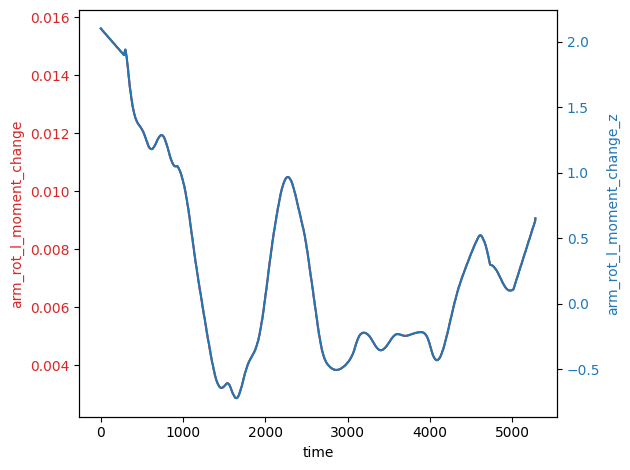
\includegraphics{03_TS_processing/02_TS_processing_acoustics_final_files/figure-pdf/cell-8-output-1.pdf}

Now we loop over all the audio files and extract the vocalic energy

\begin{Shaded}
\begin{Highlighting}[]
\CommentTok{\# Loop over wav files}
\ControlFlowTok{for}\NormalTok{ audiofile }\KeywordTok{in}\NormalTok{ actotrack:}

    \CommentTok{\# get the trialid}
\NormalTok{    trialid }\OperatorTok{=}\NormalTok{ audiofile.split(}\StringTok{\textquotesingle{}}\CharTok{\textbackslash{}\textbackslash{}}\StringTok{\textquotesingle{}}\NormalTok{)[}\OperatorTok{{-}}\DecValTok{1}\NormalTok{].split(}\StringTok{\textquotesingle{}.\textquotesingle{}}\NormalTok{)[}\DecValTok{0}\NormalTok{]}
\NormalTok{    trialid }\OperatorTok{=} \StringTok{\textquotesingle{}\_\textquotesingle{}}\NormalTok{.join(trialid.split(}\StringTok{\textquotesingle{}\_\textquotesingle{}}\NormalTok{)[}\DecValTok{0}\NormalTok{:}\DecValTok{1}\NormalTok{] }\OperatorTok{+}\NormalTok{ trialid.split(}\StringTok{\textquotesingle{}\_\textquotesingle{}}\NormalTok{)[}\DecValTok{1}\NormalTok{:}\DecValTok{2}\NormalTok{] }\OperatorTok{+}\NormalTok{ trialid.split(}\StringTok{\textquotesingle{}\_\textquotesingle{}}\NormalTok{)[}\DecValTok{3}\NormalTok{:}\DecValTok{4}\NormalTok{] }\OperatorTok{+}\NormalTok{ trialid.split(}\StringTok{\textquotesingle{}\_\textquotesingle{}}\NormalTok{)[}\DecValTok{7}\NormalTok{:}\DecValTok{8}\NormalTok{])}

    \BuiltInTok{print}\NormalTok{(}\StringTok{\textquotesingle{}working on \textquotesingle{}} \OperatorTok{+}\NormalTok{ trialid)}

    \CommentTok{\# apply the function}
\NormalTok{    ampv, sr }\OperatorTok{=}\NormalTok{ amp\_envelope(audiofile)}

    \CommentTok{\# Extract and plot the original signal}
\NormalTok{    rawaudio, sr }\OperatorTok{=}\NormalTok{ librosa.load(audiofile, sr}\OperatorTok{=}\VariableTok{None}\NormalTok{)}

    \CommentTok{\# create a time vector}
\NormalTok{    time\_env }\OperatorTok{=}\NormalTok{ np.arange(}\DecValTok{0}\NormalTok{, }\BuiltInTok{len}\NormalTok{(rawaudio)}\OperatorTok{/}\NormalTok{sr, }\DecValTok{1}\OperatorTok{/}\NormalTok{sr)}
    
    \CommentTok{\# Ensure the lengths match by padding ampv if necessary (Note that is a quick fix)}
    \ControlFlowTok{if} \BuiltInTok{len}\NormalTok{(ampv) }\OperatorTok{\textless{}} \BuiltInTok{len}\NormalTok{(time\_env):}
\NormalTok{        ampv }\OperatorTok{=}\NormalTok{ np.pad(ampv, (}\DecValTok{0}\NormalTok{, }\BuiltInTok{len}\NormalTok{(time\_env) }\OperatorTok{{-}} \BuiltInTok{len}\NormalTok{(ampv)), mode}\OperatorTok{=}\StringTok{\textquotesingle{}constant\textquotesingle{}}\NormalTok{)}
    \ControlFlowTok{elif} \BuiltInTok{len}\NormalTok{(ampv) }\OperatorTok{\textgreater{}} \BuiltInTok{len}\NormalTok{(time\_env):}
\NormalTok{        ampv }\OperatorTok{=}\NormalTok{ ampv[:}\BuiltInTok{len}\NormalTok{(time\_env)]}

    \CommentTok{\# the same for rawaudio}
    \ControlFlowTok{if} \BuiltInTok{len}\NormalTok{(rawaudio) }\OperatorTok{\textless{}} \BuiltInTok{len}\NormalTok{(time\_env):}
\NormalTok{        rawaudio }\OperatorTok{=}\NormalTok{ np.pad(rawaudio, (}\DecValTok{0}\NormalTok{, }\BuiltInTok{len}\NormalTok{(time\_env) }\OperatorTok{{-}} \BuiltInTok{len}\NormalTok{(rawaudio)), mode}\OperatorTok{=}\StringTok{\textquotesingle{}constant\textquotesingle{}}\NormalTok{)}
    \ControlFlowTok{elif} \BuiltInTok{len}\NormalTok{(rawaudio) }\OperatorTok{\textgreater{}} \BuiltInTok{len}\NormalTok{(time\_env):}
\NormalTok{        rawaudio }\OperatorTok{=}\NormalTok{ rawaudio[:}\BuiltInTok{len}\NormalTok{(time\_env)]}
    
    \CommentTok{\# save the audio and envelope}
    \ControlFlowTok{try}\NormalTok{:}
\NormalTok{        audio }\OperatorTok{=}\NormalTok{ pd.DataFrame(\{}\StringTok{\textquotesingle{}time\textquotesingle{}}\NormalTok{: time\_env, }\StringTok{\textquotesingle{}audio\textquotesingle{}}\NormalTok{: rawaudio, }\StringTok{\textquotesingle{}envelope\textquotesingle{}}\NormalTok{: ampv, }\StringTok{\textquotesingle{}trialID\textquotesingle{}}\NormalTok{: trialid\})}
        \CommentTok{\# convert time to ms}
\NormalTok{        audio[}\StringTok{\textquotesingle{}time\textquotesingle{}}\NormalTok{] }\OperatorTok{=}\NormalTok{ audio[}\StringTok{\textquotesingle{}time\textquotesingle{}}\NormalTok{] }\OperatorTok{*} \DecValTok{1000}

        \CommentTok{\# perform also envelope change}
\NormalTok{        audio[}\StringTok{\textquotesingle{}envelope\_change\textquotesingle{}}\NormalTok{] }\OperatorTok{=}\NormalTok{ np.insert(np.diff(audio[}\StringTok{\textquotesingle{}envelope\textquotesingle{}}\NormalTok{]), }\DecValTok{0}\NormalTok{, }\DecValTok{0}\NormalTok{)}
        \CommentTok{\# smooth}
\NormalTok{        audio[}\StringTok{\textquotesingle{}envelope\_change\textquotesingle{}}\NormalTok{] }\OperatorTok{=}\NormalTok{ butter\_lowpass\_filtfilt(np.}\BuiltInTok{abs}\NormalTok{(audio[}\StringTok{\textquotesingle{}envelope\_change\textquotesingle{}}\NormalTok{]), }\DecValTok{10}\NormalTok{, sr, order}\OperatorTok{=}\DecValTok{2}\NormalTok{)}
        
        \CommentTok{\# write as csv}
\NormalTok{        audio.to\_csv(ACfolder\_processed }\OperatorTok{+} \StringTok{\textquotesingle{}/env\_\textquotesingle{}} \OperatorTok{+}\NormalTok{ trialid }\OperatorTok{+} \StringTok{\textquotesingle{}.csv\textquotesingle{}}\NormalTok{, index}\OperatorTok{=}\VariableTok{False}\NormalTok{)}

    \ControlFlowTok{except} \PreprocessorTok{ValueError}\NormalTok{:}
        \BuiltInTok{print}\NormalTok{(}\StringTok{\textquotesingle{}ValueError: \textquotesingle{}} \OperatorTok{+}\NormalTok{ trialid)}
        \ControlFlowTok{continue}
\end{Highlighting}
\end{Shaded}

This is an example of a file

\begin{longtable}[]{@{}llllll@{}}
\toprule\noalign{}
& time & audio & envelope & trialID & envelope\_change \\
\midrule\noalign{}
\endhead
\bottomrule\noalign{}
\endlastfoot
0 & 0.000000 & -0.000031 & 0.016587 & 0\_1\_18\_p0 & -4.792690e-09 \\
1 & 0.020833 & -0.000031 & 0.016587 & 0\_1\_18\_p0 & -4.779707e-09 \\
2 & 0.041667 & -0.000031 & 0.016587 & 0\_1\_18\_p0 & -4.766729e-09 \\
3 & 0.062500 & -0.000031 & 0.016587 & 0\_1\_18\_p0 & -4.753755e-09 \\
4 & 0.083333 & -0.000031 & 0.016587 & 0\_1\_18\_p0 & -4.740787e-09 \\
5 & 0.104167 & -0.000031 & 0.016587 & 0\_1\_18\_p0 & -4.727823e-09 \\
6 & 0.125000 & -0.000031 & 0.016587 & 0\_1\_18\_p0 & -4.714864e-09 \\
7 & 0.145833 & -0.000031 & 0.016587 & 0\_1\_18\_p0 & -4.701909e-09 \\
8 & 0.166667 & -0.000031 & 0.016587 & 0\_1\_18\_p0 & -4.688959e-09 \\
9 & 0.187500 & -0.000031 & 0.016587 & 0\_1\_18\_p0 & -4.676015e-09 \\
10 & 0.208333 & -0.000031 & 0.016587 & 0\_1\_18\_p0 & -4.663075e-09 \\
11 & 0.229167 & -0.000031 & 0.016587 & 0\_1\_18\_p0 & -4.650139e-09 \\
12 & 0.250000 & -0.000031 & 0.016587 & 0\_1\_18\_p0 & -4.637209e-09 \\
13 & 0.270833 & 0.000000 & 0.016587 & 0\_1\_18\_p0 & -4.624284e-09 \\
14 & 0.291667 & 0.000000 & 0.016587 & 0\_1\_18\_p0 & -4.611364e-09 \\
\end{longtable}

Here it is visualized

\includegraphics{03_TS_processing/02_TS_processing_acoustics_final_files/figure-pdf/cell-11-output-1.pdf}

\bookmarksetup{startatroot}

\chapter{Extracting fundamental frequency
(f0)}\label{extracting-fundamental-frequency-f0}

Now we extract pitch using the \texttt{parselmouth} library.

Because we need take into consideration the sex of participant to set
the f0 range accordingly, prior to this script we have extracted the
speakers' register using Praat script
\texttt{Get\_Speakers\_register.praat} from Celine De Looze and save it
in file \emph{SpekaerRegister.txt}.

Now, we first check the mean min and max f0 values across all available
data and set the range accordingly.

\begin{Shaded}
\begin{Highlighting}[]
\CommentTok{\# this is where we store the min{-}max f0 values of each speaker}
\NormalTok{register }\OperatorTok{=}\NormalTok{ pd.read\_csv(curfolder }\OperatorTok{+} \StringTok{\textquotesingle{}}\CharTok{\textbackslash{}\textbackslash{}}\StringTok{SpeakerRegister.txt\textquotesingle{}}\NormalTok{, sep}\OperatorTok{=}\StringTok{\textquotesingle{}}\CharTok{\textbackslash{}t}\StringTok{\textquotesingle{}}\NormalTok{) }

\CommentTok{\# here we store metadata for each session about sex}
\NormalTok{meta }\OperatorTok{=}\NormalTok{ pd.read\_csv(curfolder }\OperatorTok{+} \StringTok{\textquotesingle{}}\CharTok{\textbackslash{}\textbackslash{}}\StringTok{..}\CharTok{\textbackslash{}\textbackslash{}}\StringTok{00\_RAWDATA}\CharTok{\textbackslash{}\textbackslash{}}\StringTok{META\_gender.txt\textquotesingle{}}\NormalTok{, sep}\OperatorTok{=}\StringTok{\textquotesingle{}}\CharTok{\textbackslash{}t}\StringTok{\textquotesingle{}}\NormalTok{)}

\CommentTok{\# now we want to find out the range for males and females}
\NormalTok{register[}\StringTok{\textquotesingle{}sex\textquotesingle{}}\NormalTok{] }\OperatorTok{=} \VariableTok{None}

\CommentTok{\# make f0min and f0max numeric}
\NormalTok{register[}\StringTok{\textquotesingle{}f0min\textquotesingle{}}\NormalTok{] }\OperatorTok{=}\NormalTok{ pd.to\_numeric(register[}\StringTok{\textquotesingle{}f0min\textquotesingle{}}\NormalTok{], errors}\OperatorTok{=}\StringTok{\textquotesingle{}coerce\textquotesingle{}}\NormalTok{)}
\NormalTok{register[}\StringTok{\textquotesingle{}f0max\textquotesingle{}}\NormalTok{] }\OperatorTok{=}\NormalTok{ pd.to\_numeric(register[}\StringTok{\textquotesingle{}f0max\textquotesingle{}}\NormalTok{], errors}\OperatorTok{=}\StringTok{\textquotesingle{}coerce\textquotesingle{}}\NormalTok{)}

\CommentTok{\# loop over rows in register,}
\ControlFlowTok{for}\NormalTok{ idx, row }\KeywordTok{in}\NormalTok{ register.iterrows():}
    \CommentTok{\#  get sessionID from FILE (first part)}
\NormalTok{    sessionID }\OperatorTok{=}\NormalTok{ row[}\StringTok{\textquotesingle{}FILE\textquotesingle{}}\NormalTok{].split(}\StringTok{\textquotesingle{}\_\textquotesingle{}}\NormalTok{)[}\DecValTok{0}\NormalTok{]}
    \CommentTok{\# get pcn id}
\NormalTok{    pcn }\OperatorTok{=}\NormalTok{ row[}\StringTok{\textquotesingle{}FILE\textquotesingle{}}\NormalTok{].split(}\StringTok{\textquotesingle{}\_\textquotesingle{}}\NormalTok{)[}\DecValTok{7}\NormalTok{]}
    \CommentTok{\# merge it}
\NormalTok{    ID }\OperatorTok{=}\NormalTok{ sessionID }\OperatorTok{+} \StringTok{\textquotesingle{}\_\textquotesingle{}} \OperatorTok{+}\NormalTok{ pcn}
    \CommentTok{\# find this id in meta and save in sex the value in column sex}
\NormalTok{    sex }\OperatorTok{=}\NormalTok{ meta[meta[}\StringTok{\textquotesingle{}ID\textquotesingle{}}\NormalTok{] }\OperatorTok{==}\NormalTok{ ID][}\StringTok{\textquotesingle{}sex\textquotesingle{}}\NormalTok{].values[}\DecValTok{0}\NormalTok{]}
    \CommentTok{\# save value of sex in current row}
\NormalTok{    register.at[idx, }\StringTok{\textquotesingle{}sex\textquotesingle{}}\NormalTok{] }\OperatorTok{=}\NormalTok{ sex}

\CommentTok{\# now group sex by each value and find the mean of f0min and f0max}
\NormalTok{f0min }\OperatorTok{=}\NormalTok{ register.groupby(}\StringTok{\textquotesingle{}sex\textquotesingle{}}\NormalTok{)[}\StringTok{\textquotesingle{}f0min\textquotesingle{}}\NormalTok{].}\BuiltInTok{min}\NormalTok{()}
\NormalTok{f0max }\OperatorTok{=}\NormalTok{ register.groupby(}\StringTok{\textquotesingle{}sex\textquotesingle{}}\NormalTok{)[}\StringTok{\textquotesingle{}f0max\textquotesingle{}}\NormalTok{].mean()}
\BuiltInTok{print}\NormalTok{(f0min, f0max)}
\end{Highlighting}
\end{Shaded}

\begin{verbatim}
sex
f    22.0
Name: f0min, dtype: float64 sex
f    380.660131
Name: f0max, dtype: float64
\end{verbatim}

Dyad 0 consists of two females, and the f0 min is 22 Hz and f0 maxis 381
Hz.

\begin{Shaded}
\begin{Highlighting}[]
\KeywordTok{def}\NormalTok{ extract\_f0(locationsound, sex):}

    \CommentTok{\# read the sound file as numpy array}
\NormalTok{    audio, sr }\OperatorTok{=}\NormalTok{ librosa.load(locationsound, sr}\OperatorTok{=}\DecValTok{48000}\NormalTok{)}

    \CommentTok{\# read the sound file into Python}
\NormalTok{    snd }\OperatorTok{=}\NormalTok{ parselmouth.Sound(audio, sampling\_frequency}\OperatorTok{=}\NormalTok{sr)}

    \ControlFlowTok{if}\NormalTok{ sex }\OperatorTok{==} \StringTok{\textquotesingle{}f\textquotesingle{}}\NormalTok{:}
\NormalTok{        f0min }\OperatorTok{=} \DecValTok{22}      \CommentTok{\#\# calculated by previous chunk}
\NormalTok{        f0max }\OperatorTok{=} \DecValTok{381}
    \ControlFlowTok{else}\NormalTok{:}
\NormalTok{        f0min }\OperatorTok{=} \DecValTok{30}      \CommentTok{\#\# Note: don\textquotesingle{}t have any males in dyad0 so this is only placeholder}
\NormalTok{        f0max }\OperatorTok{=} \DecValTok{650}

\NormalTok{    pitch }\OperatorTok{=}\NormalTok{ snd.to\_pitch(time\_step }\OperatorTok{=} \FloatTok{0.002}\NormalTok{, pitch\_floor}\OperatorTok{=}\NormalTok{f0min, pitch\_ceiling}\OperatorTok{=}\NormalTok{f0max) }\CommentTok{\#time\_step to get 500Hz}

\NormalTok{    f0\_values }\OperatorTok{=}\NormalTok{ pitch.selected\_array[}\StringTok{\textquotesingle{}frequency\textquotesingle{}}\NormalTok{]}

    \ControlFlowTok{return}\NormalTok{ snd, f0\_values}
\end{Highlighting}
\end{Shaded}

Now we loop over all audio files and extract f0 from each. Resulting f0
contours were smoothed with a Savitzky-Golay 3rd-polynomial filter with
a span of 50 ms (following (\textbf{ADDREF?})) applied to continuous
runs of phonated vocalization to maintain discontinuities typical of the
f0 signal.

\begin{Shaded}
\begin{Highlighting}[]
\NormalTok{freq}\OperatorTok{=}\DecValTok{48000}    
\NormalTok{meta }\OperatorTok{=}\NormalTok{ pd.read\_csv(curfolder }\OperatorTok{+} \StringTok{\textquotesingle{}}\CharTok{\textbackslash{}\textbackslash{}}\StringTok{..}\CharTok{\textbackslash{}\textbackslash{}}\StringTok{00\_RAWDATA}\CharTok{\textbackslash{}\textbackslash{}}\StringTok{META.txt\textquotesingle{}}\NormalTok{, sep}\OperatorTok{=}\StringTok{\textquotesingle{}}\CharTok{\textbackslash{}t}\StringTok{\textquotesingle{}}\NormalTok{)}

\CommentTok{\# Loop over wav files}
\ControlFlowTok{for}\NormalTok{ audiofile }\KeywordTok{in}\NormalTok{ actotrack:}

    \CommentTok{\# get the trialid}
\NormalTok{    trialid }\OperatorTok{=}\NormalTok{ audiofile.split(}\StringTok{\textquotesingle{}}\CharTok{\textbackslash{}\textbackslash{}}\StringTok{\textquotesingle{}}\NormalTok{)[}\OperatorTok{{-}}\DecValTok{1}\NormalTok{].split(}\StringTok{\textquotesingle{}.\textquotesingle{}}\NormalTok{)[}\DecValTok{0}\NormalTok{]}
    \CommentTok{\#trial id is the first, second, fourth and eighth element}
\NormalTok{    trialid }\OperatorTok{=} \StringTok{\textquotesingle{}\_\textquotesingle{}}\NormalTok{.join(trialid.split(}\StringTok{\textquotesingle{}\_\textquotesingle{}}\NormalTok{)[}\DecValTok{0}\NormalTok{:}\DecValTok{1}\NormalTok{] }\OperatorTok{+}\NormalTok{ trialid.split(}\StringTok{\textquotesingle{}\_\textquotesingle{}}\NormalTok{)[}\DecValTok{1}\NormalTok{:}\DecValTok{2}\NormalTok{] }\OperatorTok{+}\NormalTok{ trialid.split(}\StringTok{\textquotesingle{}\_\textquotesingle{}}\NormalTok{)[}\DecValTok{3}\NormalTok{:}\DecValTok{4}\NormalTok{] }\OperatorTok{+}\NormalTok{ trialid.split(}\StringTok{\textquotesingle{}\_\textquotesingle{}}\NormalTok{)[}\DecValTok{7}\NormalTok{:}\DecValTok{8}\NormalTok{])}

    \BuiltInTok{print}\NormalTok{(}\StringTok{\textquotesingle{}working on \textquotesingle{}} \OperatorTok{+}\NormalTok{ trialid)}

    \CommentTok{\# first element is sessionid, fourth element is participantid}
\NormalTok{    sessionid }\OperatorTok{=}\NormalTok{ trialid.split(}\StringTok{\textquotesingle{}\_\textquotesingle{}}\NormalTok{)[}\DecValTok{0}\NormalTok{]}
\NormalTok{    participantid }\OperatorTok{=}\NormalTok{ trialid.split(}\StringTok{\textquotesingle{}\_\textquotesingle{}}\NormalTok{)[}\DecValTok{3}\NormalTok{]}
\NormalTok{    ID }\OperatorTok{=}\NormalTok{ sessionid }\OperatorTok{+} \StringTok{\textquotesingle{}\_\textquotesingle{}} \OperatorTok{+}\NormalTok{ participantid}

    \CommentTok{\# what sex has this ID in meta}
\NormalTok{    sex }\OperatorTok{=}\NormalTok{ meta[meta[}\StringTok{\textquotesingle{}ID\textquotesingle{}}\NormalTok{] }\OperatorTok{==}\NormalTok{ ID][}\StringTok{\textquotesingle{}sex\textquotesingle{}}\NormalTok{].values[}\DecValTok{0}\NormalTok{]}

    \CommentTok{\# apply the function}
\NormalTok{    snd, f0 }\OperatorTok{=}\NormalTok{ extract\_f0(audiofile, sex)}

\NormalTok{    length }\OperatorTok{=} \BuiltInTok{len}\NormalTok{(f0)}

    \CommentTok{\# replace 0 values with NaN}
\NormalTok{    f0 }\OperatorTok{=}\NormalTok{ np.where(f0 }\OperatorTok{==} \DecValTok{0}\NormalTok{, np.nan, f0)}

    \CommentTok{\# create time vector}
\NormalTok{    F0\_time }\OperatorTok{=}\NormalTok{ np.linspace(}\DecValTok{0}\NormalTok{, snd.duration, }\BuiltInTok{len}\NormalTok{(f0)) }\OperatorTok{*} \DecValTok{1000}  \CommentTok{\# Generate time vector}

    \CommentTok{\# create df}
\NormalTok{    f0\_df }\OperatorTok{=}\NormalTok{ pd.DataFrame(\{}\StringTok{\textquotesingle{}time\_ms\textquotesingle{}}\NormalTok{: F0\_time, }\StringTok{\textquotesingle{}f0\textquotesingle{}}\NormalTok{: f0, }\StringTok{\textquotesingle{}ID\textquotesingle{}}\NormalTok{: trialid\})}

    \CommentTok{\# Smooth the f0 values}
    \ControlFlowTok{try}\NormalTok{:}
\NormalTok{        f0\_df }\OperatorTok{=}\NormalTok{ chunk\_and\_smooth(f0\_df, }\StringTok{\textquotesingle{}f0\textquotesingle{}}\NormalTok{) }\CommentTok{\# do it with window 25}
    \ControlFlowTok{except} \PreprocessorTok{ValueError}\NormalTok{:}
        \CommentTok{\# unless there is only tiny chunk of f0 and then we need window of 5}
        \BuiltInTok{print}\NormalTok{(}\StringTok{\textquotesingle{}ValueError: \textquotesingle{}} \OperatorTok{+}\NormalTok{ trialid }\OperatorTok{+} \StringTok{\textquotesingle{}, f0 trace is smaller than window length, resuming to window=5\textquotesingle{}}\NormalTok{)}
\NormalTok{        f0\_df }\OperatorTok{=}\NormalTok{ chunk\_and\_smooth(f0\_df, }\StringTok{\textquotesingle{}f0\textquotesingle{}}\NormalTok{, window}\OperatorTok{=}\DecValTok{5}\NormalTok{)}

    \CommentTok{\# write as csv}
\NormalTok{    f0\_df.to\_csv(ACfolder\_processed }\OperatorTok{+} \StringTok{\textquotesingle{}/f0\_\textquotesingle{}} \OperatorTok{+}\NormalTok{ trialid }\OperatorTok{+} \StringTok{\textquotesingle{}.csv\textquotesingle{}}\NormalTok{, index}\OperatorTok{=}\VariableTok{False}\NormalTok{)}
\end{Highlighting}
\end{Shaded}

Here is an example of a file

\begin{longtable}[]{@{}llll@{}}
\toprule\noalign{}
& time\_ms & f0 & ID \\
\midrule\noalign{}
\endhead
\bottomrule\noalign{}
\endlastfoot
0 & 0.000000 & NaN & 0\_1\_10\_p1 \\
1 & 2.052699 & NaN & 0\_1\_10\_p1 \\
2 & 4.105398 & NaN & 0\_1\_10\_p1 \\
3 & 6.158097 & NaN & 0\_1\_10\_p1 \\
4 & 8.210796 & NaN & 0\_1\_10\_p1 \\
5 & 10.263495 & NaN & 0\_1\_10\_p1 \\
6 & 12.316194 & NaN & 0\_1\_10\_p1 \\
7 & 14.368892 & NaN & 0\_1\_10\_p1 \\
8 & 16.421591 & NaN & 0\_1\_10\_p1 \\
9 & 18.474290 & NaN & 0\_1\_10\_p1 \\
10 & 20.526989 & NaN & 0\_1\_10\_p1 \\
11 & 22.579688 & NaN & 0\_1\_10\_p1 \\
12 & 24.632387 & NaN & 0\_1\_10\_p1 \\
13 & 26.685086 & NaN & 0\_1\_10\_p1 \\
14 & 28.737785 & NaN & 0\_1\_10\_p1 \\
\end{longtable}

And here visualized

\includegraphics{03_TS_processing/02_TS_processing_acoustics_final_files/figure-pdf/cell-16-output-1.pdf}

\bookmarksetup{startatroot}

\chapter{Extracting spectral
centroid}\label{extracting-spectral-centroid}

To extract the are of the main spectral energy, we will compute spectral
centroid / spectral center of gravity using \texttt{parselmouth}
package. We are filtering out the fundamental frequency (F0) to remove
low-frequency components that might interfere with the analysis (code
adapted from
\href{https://se.mathworks.com/matlabcentral/fileexchange/104555-digital-signal-processing-system-analysis-and-design?focused=b988de35-99f5-4f66-a67f-c014b9c170b1&tab=function}{here}).

\begin{Shaded}
\begin{Highlighting}[]
\ImportTok{from}\NormalTok{ scipy.signal }\ImportTok{import}\NormalTok{ sosfilt}

\KeywordTok{def}\NormalTok{ remove\_f0(x, fundamental, fs):}
    \CommentTok{\# Normalize the frequency for digital filter design}
\NormalTok{    f\_dig }\OperatorTok{=} \DecValTok{2} \OperatorTok{*}\NormalTok{ np.pi }\OperatorTok{*}\NormalTok{ fundamental }\OperatorTok{/}\NormalTok{ fs}
    
    \CommentTok{\# Define the notch filter parameters for F0}
\NormalTok{    p1 }\OperatorTok{=} \FloatTok{0.999} \OperatorTok{*}\NormalTok{ np.exp(}\OtherTok{1j} \OperatorTok{*}\NormalTok{ f\_dig)  }\CommentTok{\# Pole near the F0 frequency}
\NormalTok{    z1 }\OperatorTok{=}\NormalTok{ np.exp(}\OtherTok{1j} \OperatorTok{*}\NormalTok{ f\_dig)          }\CommentTok{\# Zero near the F0 frequency}
    
    \CommentTok{\# Define zeros and poles for the notch filter}
\NormalTok{    zeros }\OperatorTok{=}\NormalTok{ np.array([z1, z1])}
\NormalTok{    poles }\OperatorTok{=}\NormalTok{ np.array([p1, p1])}
    
    \CommentTok{\# Create a 2nd{-}order section (sos) filter array}
\NormalTok{    sos }\OperatorTok{=}\NormalTok{ np.array([[}\DecValTok{1}\NormalTok{, }\OperatorTok{{-}}\DecValTok{2} \OperatorTok{*}\NormalTok{ np.real(p1), }\DecValTok{1}\NormalTok{, }\DecValTok{1}\NormalTok{, }\OperatorTok{{-}}\DecValTok{2} \OperatorTok{*}\NormalTok{ np.real(z1), np.}\BuiltInTok{abs}\NormalTok{(z1)}\OperatorTok{**}\DecValTok{2}\NormalTok{]])}

    \CommentTok{\# Apply the notch filter to the signal}
\NormalTok{    y }\OperatorTok{=}\NormalTok{ sosfilt(sos, x)}
    
    \ControlFlowTok{return}\NormalTok{ y}
\end{Highlighting}
\end{Shaded}

\begin{Shaded}
\begin{Highlighting}[]
\CommentTok{\# Parameters}
\NormalTok{window\_length }\OperatorTok{=} \FloatTok{0.03} \CommentTok{\# 30ms analysis window}

\CommentTok{\# Loop over wav files}
\ControlFlowTok{for}\NormalTok{ audiofile }\KeywordTok{in}\NormalTok{ actotrack:}
    \CommentTok{\# Extract trial ID from filename}
\NormalTok{    trialid }\OperatorTok{=}\NormalTok{ os.path.basename(audiofile).split(}\StringTok{\textquotesingle{}.\textquotesingle{}}\NormalTok{)[}\DecValTok{0}\NormalTok{]}
\NormalTok{    trialid }\OperatorTok{=} \StringTok{\textquotesingle{}\_\textquotesingle{}}\NormalTok{.join(trialid.split(}\StringTok{\textquotesingle{}\_\textquotesingle{}}\NormalTok{)[}\DecValTok{0}\NormalTok{:}\DecValTok{1}\NormalTok{] }\OperatorTok{+}\NormalTok{ trialid.split(}\StringTok{\textquotesingle{}\_\textquotesingle{}}\NormalTok{)[}\DecValTok{1}\NormalTok{:}\DecValTok{2}\NormalTok{] }\OperatorTok{+}\NormalTok{ trialid.split(}\StringTok{\textquotesingle{}\_\textquotesingle{}}\NormalTok{)[}\DecValTok{3}\NormalTok{:}\DecValTok{4}\NormalTok{] }\OperatorTok{+}\NormalTok{ trialid.split(}\StringTok{\textquotesingle{}\_\textquotesingle{}}\NormalTok{)[}\DecValTok{7}\NormalTok{:}\DecValTok{8}\NormalTok{])}

    \BuiltInTok{print}\NormalTok{(}\SpecialStringTok{f\textquotesingle{}Working on }\SpecialCharTok{\{}\NormalTok{trialid}\SpecialCharTok{\}}\SpecialStringTok{\textquotesingle{}}\NormalTok{)}

    \CommentTok{\# Extract session and participant ID}
\NormalTok{    sessionid }\OperatorTok{=}\NormalTok{ trialid.split(}\StringTok{\textquotesingle{}\_\textquotesingle{}}\NormalTok{)[}\DecValTok{0}\NormalTok{]}
\NormalTok{    participantid }\OperatorTok{=}\NormalTok{ trialid.split(}\StringTok{\textquotesingle{}\_\textquotesingle{}}\NormalTok{)[}\DecValTok{3}\NormalTok{]}
\NormalTok{    ID }\OperatorTok{=} \SpecialStringTok{f"}\SpecialCharTok{\{}\NormalTok{sessionid}\SpecialCharTok{\}}\SpecialStringTok{\_}\SpecialCharTok{\{}\NormalTok{participantid}\SpecialCharTok{\}}\SpecialStringTok{"}

    \CommentTok{\# Load sound}
\NormalTok{    snd }\OperatorTok{=}\NormalTok{ parselmouth.Sound(audiofile)}

    \CommentTok{\# Get sampling rate}
\NormalTok{    fs }\OperatorTok{=}\NormalTok{ snd.sampling\_frequency}

    \CommentTok{\# Load f0 file with the same trialid}
\NormalTok{    f0file }\OperatorTok{=}\NormalTok{ ACfolder\_processed }\OperatorTok{+} \StringTok{\textquotesingle{}/f0\_\textquotesingle{}} \OperatorTok{+}\NormalTok{ trialid }\OperatorTok{+} \StringTok{\textquotesingle{}.csv\textquotesingle{}}
\NormalTok{    f0\_df }\OperatorTok{=}\NormalTok{ pd.read\_csv(f0file)}

    \CommentTok{\# Get the mean (from non{-}NaN values) of the f0}
\NormalTok{    f0\_df }\OperatorTok{=}\NormalTok{ f0\_df.dropna()}
\NormalTok{    mean\_f0 }\OperatorTok{=}\NormalTok{ f0\_df[}\StringTok{\textquotesingle{}f0\textquotesingle{}}\NormalTok{].mean()}

    \CommentTok{\# Sound values}
\NormalTok{    sound\_values }\OperatorTok{=}\NormalTok{ snd.values[}\DecValTok{0}\NormalTok{]}

    \CommentTok{\# Remove F0 from the signal using the mean F0}
\NormalTok{    filtered\_signal }\OperatorTok{=}\NormalTok{ remove\_f0(sound\_values, mean\_f0, fs)}

    \CommentTok{\# Recreate the sound object with the filtered signal}
\NormalTok{    filtered\_sound }\OperatorTok{=}\NormalTok{ parselmouth.Sound(filtered\_signal, sampling\_frequency}\OperatorTok{=}\NormalTok{fs)}

    \CommentTok{\# Compute spectrogram of the filtered signal}
\NormalTok{    spectrogram }\OperatorTok{=}\NormalTok{ filtered\_sound.to\_spectrogram(window\_length}\OperatorTok{=}\NormalTok{window\_length)}

    \CommentTok{\# Extract time values from the spectrogram}
\NormalTok{    times }\OperatorTok{=}\NormalTok{ spectrogram.xs()  }\CommentTok{\# Time vector in seconds}

    \CommentTok{\# Compute CoG for each time step}
\NormalTok{    cog\_values }\OperatorTok{=}\NormalTok{ [spectrogram.to\_spectrum\_slice(time}\OperatorTok{=}\NormalTok{t).get\_centre\_of\_gravity(power}\OperatorTok{=}\FloatTok{2.0}\NormalTok{) }\ControlFlowTok{for}\NormalTok{ t }\KeywordTok{in}\NormalTok{ times]}

    \CommentTok{\# Convert time to milliseconds}
\NormalTok{    time\_cog }\OperatorTok{=}\NormalTok{ np.array(times) }\OperatorTok{*} \DecValTok{1000}  

    \CommentTok{\# Convert CoG values to numpy array}
\NormalTok{    cog\_values }\OperatorTok{=}\NormalTok{ np.array(cog\_values)}

    \CommentTok{\# Create DataFrame}
\NormalTok{    cog\_df }\OperatorTok{=}\NormalTok{ pd.DataFrame(\{}\StringTok{\textquotesingle{}time\textquotesingle{}}\NormalTok{: time\_cog, }\StringTok{\textquotesingle{}CoG\textquotesingle{}}\NormalTok{: cog\_values, }\StringTok{\textquotesingle{}TrialID\textquotesingle{}}\NormalTok{: trialid\})}

    \CommentTok{\# Replace zeros with NaN}
\NormalTok{    cog\_df[}\StringTok{\textquotesingle{}CoG\textquotesingle{}}\NormalTok{] }\OperatorTok{=}\NormalTok{ cog\_df[}\StringTok{\textquotesingle{}CoG\textquotesingle{}}\NormalTok{].replace(}\DecValTok{0}\NormalTok{, np.nan)}

    \CommentTok{\# Smooth the data}
    \ControlFlowTok{try}\NormalTok{:}
\NormalTok{        cog\_df }\OperatorTok{=}\NormalTok{ chunk\_and\_smooth(cog\_df, }\StringTok{\textquotesingle{}CoG\textquotesingle{}}\NormalTok{)}
    \ControlFlowTok{except} \PreprocessorTok{ValueError}\NormalTok{:}
        \BuiltInTok{print}\NormalTok{(}\SpecialStringTok{f\textquotesingle{}ValueError: }\SpecialCharTok{\{}\NormalTok{trialid}\SpecialCharTok{\}}\SpecialStringTok{, CoG trace is smaller than window length, using window=5\textquotesingle{}}\NormalTok{)}
\NormalTok{        cog\_df }\OperatorTok{=}\NormalTok{ chunk\_and\_smooth(cog\_df, }\StringTok{\textquotesingle{}CoG\textquotesingle{}}\NormalTok{, window}\OperatorTok{=}\DecValTok{5}\NormalTok{)}

    \CommentTok{\# Save DataFrame}
\NormalTok{    output\_path }\OperatorTok{=}\NormalTok{ os.path.join(ACfolder\_processed, }\SpecialStringTok{f\textquotesingle{}cog\_}\SpecialCharTok{\{}\NormalTok{trialid}\SpecialCharTok{\}}\SpecialStringTok{.csv\textquotesingle{}}\NormalTok{)}
\NormalTok{    cog\_df.to\_csv(output\_path, index}\OperatorTok{=}\VariableTok{False}\NormalTok{)}
\end{Highlighting}
\end{Shaded}

This is a visual example of a file

\includegraphics{03_TS_processing/02_TS_processing_acoustics_final_files/figure-pdf/cell-19-output-1.pdf}

\bookmarksetup{startatroot}

\chapter{Extracting formants}\label{extracting-formants}

To extract formant values, we use Chris Carignan's Praat script (see
\href{https://github.com/ChristopherCarignan/formant-optimization}{Github})
which optimizes the F1-F5 values.

To verify the sensibility of the data, we will do some visual
inspections. Moreover, we will consider taking formant values from the
windows of envelope amplitude peaks.

\begin{Shaded}
\begin{Highlighting}[]
\CommentTok{\# Here we store formants from praat}
\NormalTok{formantfolder }\OperatorTok{=}\NormalTok{ curfolder }\OperatorTok{+} \StringTok{\textquotesingle{}/TS\_formants/Carignan\_formants/\textquotesingle{}}
\NormalTok{formants }\OperatorTok{=}\NormalTok{ glob.glob(formantfolder }\OperatorTok{+} \StringTok{\textquotesingle{}*.Table\textquotesingle{}}\NormalTok{)}

\CommentTok{\# Here we store processed envelope }
\NormalTok{envfiles }\OperatorTok{=}\NormalTok{ glob.glob(ACfolder\_processed }\OperatorTok{+} \StringTok{\textquotesingle{}/env\_*.csv\textquotesingle{}}\NormalTok{)}
\end{Highlighting}
\end{Shaded}

Chris Carignan's Praat-script outputs formants as a .Table. Let's
therefore first read these files and resave them as .csv files.

\begin{Shaded}
\begin{Highlighting}[]
\ControlFlowTok{for}\NormalTok{ formant }\KeywordTok{in}\NormalTok{ formants:}
\NormalTok{    formant\_df }\OperatorTok{=}\NormalTok{ pd.read\_csv(formant, sep}\OperatorTok{=}\StringTok{\textquotesingle{}}\CharTok{\textbackslash{}t}\StringTok{\textquotesingle{}}\NormalTok{)}

    \CommentTok{\# get the name of the file}
\NormalTok{    filename }\OperatorTok{=}\NormalTok{ os.path.basename(formant)}
    \CommentTok{\# get the name of the file without the extension}
\NormalTok{    filename }\OperatorTok{=}\NormalTok{ os.path.splitext(filename)[}\DecValTok{0}\NormalTok{]}

    \CommentTok{\# add to df}
\NormalTok{    formant\_df[}\StringTok{\textquotesingle{}filename\textquotesingle{}}\NormalTok{] }\OperatorTok{=}\NormalTok{ filename}

    \CommentTok{\# get trialid from the file name }
\NormalTok{    trialid }\OperatorTok{=} \StringTok{\textquotesingle{}\_\textquotesingle{}}\NormalTok{.join(filename.split(}\StringTok{\textquotesingle{}\_\textquotesingle{}}\NormalTok{)[}\DecValTok{0}\NormalTok{:}\DecValTok{2}\NormalTok{] }\OperatorTok{+}\NormalTok{ filename.split(}\StringTok{\textquotesingle{}\_\textquotesingle{}}\NormalTok{)[}\DecValTok{3}\NormalTok{:}\DecValTok{4}\NormalTok{] }\OperatorTok{+}\NormalTok{ filename.split(}\StringTok{\textquotesingle{}\_\textquotesingle{}}\NormalTok{)[}\DecValTok{7}\NormalTok{:}\DecValTok{8}\NormalTok{]) }

    \BuiltInTok{print}\NormalTok{(}\StringTok{\textquotesingle{}working on \textquotesingle{}} \OperatorTok{+}\NormalTok{ trialid)}

    \CommentTok{\# add empty row in the beginning with time 0 and rest as first row}
\NormalTok{    copy\_row }\OperatorTok{=}\NormalTok{ formant\_df.iloc[}\DecValTok{0}\NormalTok{].copy()}
    \CommentTok{\# time of this row is 0}
\NormalTok{    copy\_row[}\StringTok{\textquotesingle{}time\textquotesingle{}}\NormalTok{] }\OperatorTok{=} \DecValTok{0}

    \CommentTok{\# add this row to the beginning of the df}
\NormalTok{    formant\_df }\OperatorTok{=}\NormalTok{ pd.concat([pd.DataFrame(copy\_row).T, formant\_df], ignore\_index}\OperatorTok{=}\VariableTok{True}\NormalTok{)}
    
    \CommentTok{\# add trialid to the df}
\NormalTok{    formant\_df[}\StringTok{\textquotesingle{}trialid\textquotesingle{}}\NormalTok{] }\OperatorTok{=}\NormalTok{ trialid}

    \CommentTok{\# write it as csv to formantfolder1}
\NormalTok{    formant\_df.to\_csv(ACfolder\_processed }\OperatorTok{+} \StringTok{\textquotesingle{}praat\_formants\_\textquotesingle{}} \OperatorTok{+}\NormalTok{ trialid }\OperatorTok{+} \StringTok{\textquotesingle{}.csv\textquotesingle{}}\NormalTok{, index}\OperatorTok{=}\VariableTok{False}\NormalTok{)}
\end{Highlighting}
\end{Shaded}

\begin{Shaded}
\begin{Highlighting}[]
\CommentTok{\# inititate empty df}
\NormalTok{formants\_df }\OperatorTok{=}\NormalTok{ pd.DataFrame()}

\CommentTok{\# get all formant files we just created}
\NormalTok{formantfiles }\OperatorTok{=}\NormalTok{ glob.glob(ACfolder\_processed }\OperatorTok{+} \StringTok{\textquotesingle{}praat\_formants\_*.csv\textquotesingle{}}\NormalTok{)}

\CommentTok{\# loop over formants 2 and make a giga df from all}
\ControlFlowTok{for}\NormalTok{ formant }\KeywordTok{in}\NormalTok{ formantfiles:}
    \BuiltInTok{print}\NormalTok{(}\StringTok{\textquotesingle{}working on \textquotesingle{}} \OperatorTok{+}\NormalTok{ formant)}
\NormalTok{    for\_df }\OperatorTok{=}\NormalTok{ pd.read\_csv(formant)}

    \CommentTok{\# get the name of the file}
\NormalTok{    filename }\OperatorTok{=}\NormalTok{ for\_df[}\StringTok{\textquotesingle{}filename\textquotesingle{}}\NormalTok{][}\DecValTok{0}\NormalTok{]}

    \CommentTok{\# in filename, look for c1, c2, c0}
    \ControlFlowTok{if} \StringTok{\textquotesingle{}c1\textquotesingle{}} \KeywordTok{in}\NormalTok{ filename:}
\NormalTok{        for\_df[}\StringTok{\textquotesingle{}correction\textquotesingle{}}\NormalTok{] }\OperatorTok{=} \StringTok{\textquotesingle{}c1\textquotesingle{}}
    \ControlFlowTok{elif} \StringTok{\textquotesingle{}c2\textquotesingle{}} \KeywordTok{in}\NormalTok{ filename:}
\NormalTok{        for\_df[}\StringTok{\textquotesingle{}correction\textquotesingle{}}\NormalTok{] }\OperatorTok{=} \StringTok{\textquotesingle{}c2\textquotesingle{}}
    \ControlFlowTok{elif} \StringTok{\textquotesingle{}c0\textquotesingle{}} \KeywordTok{in}\NormalTok{ filename:}
\NormalTok{        for\_df[}\StringTok{\textquotesingle{}correction\textquotesingle{}}\NormalTok{] }\OperatorTok{=} \StringTok{\textquotesingle{}c0\textquotesingle{}}
    \ControlFlowTok{else}\NormalTok{:}
\NormalTok{        for\_df[}\StringTok{\textquotesingle{}correction\textquotesingle{}}\NormalTok{] }\OperatorTok{=} \StringTok{\textquotesingle{}none\textquotesingle{}}
    
    \CommentTok{\# concatenate}
\NormalTok{    formants\_df }\OperatorTok{=}\NormalTok{ pd.concat([formants\_df, for\_df])}

\CommentTok{\# get rid of rows with correction = none}
\NormalTok{formants\_df }\OperatorTok{=}\NormalTok{ formants\_df[formants\_df[}\StringTok{\textquotesingle{}correction\textquotesingle{}}\NormalTok{] }\OperatorTok{!=} \StringTok{\textquotesingle{}none\textquotesingle{}}\NormalTok{]}
\end{Highlighting}
\end{Shaded}

This is how the formants look like in a table

\begin{longtable}[]{@{}llllllllll@{}}
\toprule\noalign{}
& time & f1 & f2 & f3 & f4 & f5 & filename & trialid & correction \\
\midrule\noalign{}
\endhead
\bottomrule\noalign{}
\endlastfoot
0 & 0.000000 & 1910.072640 & 3380.992452 & 5896.442699 & 0.0 & 0.0 &
0\_2\_pr\_0\_Mic\_nominal\_srate48000\_p0\_juichen\_com... & 0\_2\_0\_p0
& c0 \\
1 & 0.026031 & 1910.072640 & 3380.992452 & 5896.442699 & 0.0 & 0.0 &
0\_2\_pr\_0\_Mic\_nominal\_srate48000\_p0\_juichen\_com... & 0\_2\_0\_p0
& c0 \\
2 & 0.031031 & 1890.080560 & 3366.165092 & 5896.610205 & 0.0 & 0.0 &
0\_2\_pr\_0\_Mic\_nominal\_srate48000\_p0\_juichen\_com... & 0\_2\_0\_p0
& c0 \\
3 & 0.036031 & 1910.066181 & 3380.974399 & 5896.442306 & 0.0 & 0.0 &
0\_2\_pr\_0\_Mic\_nominal\_srate48000\_p0\_juichen\_com... & 0\_2\_0\_p0
& c0 \\
4 & 0.041031 & 1890.092319 & 3366.156404 & 5896.609863 & 0.0 & 0.0 &
0\_2\_pr\_0\_Mic\_nominal\_srate48000\_p0\_juichen\_com... & 0\_2\_0\_p0
& c0 \\
5 & 0.046031 & 1910.073207 & 3380.962077 & 5896.441999 & 0.0 & 0.0 &
0\_2\_pr\_0\_Mic\_nominal\_srate48000\_p0\_juichen\_com... & 0\_2\_0\_p0
& c0 \\
6 & 0.051031 & 1890.087965 & 3366.149616 & 5896.609697 & 0.0 & 0.0 &
0\_2\_pr\_0\_Mic\_nominal\_srate48000\_p0\_juichen\_com... & 0\_2\_0\_p0
& c0 \\
7 & 0.056031 & 1910.062802 & 3380.953514 & 5896.441903 & 0.0 & 0.0 &
0\_2\_pr\_0\_Mic\_nominal\_srate48000\_p0\_juichen\_com... & 0\_2\_0\_p0
& c0 \\
8 & 0.061031 & 1890.085211 & 3366.138214 & 5896.609723 & 0.0 & 0.0 &
0\_2\_pr\_0\_Mic\_nominal\_srate48000\_p0\_juichen\_com... & 0\_2\_0\_p0
& c0 \\
9 & 0.066031 & 1910.063561 & 3380.941686 & 5896.442068 & 0.0 & 0.0 &
0\_2\_pr\_0\_Mic\_nominal\_srate48000\_p0\_juichen\_com... & 0\_2\_0\_p0
& c0 \\
10 & 0.071031 & 1890.080307 & 3366.122801 & 5896.610225 & 0.0 & 0.0 &
0\_2\_pr\_0\_Mic\_nominal\_srate48000\_p0\_juichen\_com... & 0\_2\_0\_p0
& c0 \\
11 & 0.076031 & 1910.048401 & 3380.925190 & 5896.443055 & 0.0 & 0.0 &
0\_2\_pr\_0\_Mic\_nominal\_srate48000\_p0\_juichen\_com... & 0\_2\_0\_p0
& c0 \\
12 & 0.081031 & 1890.073211 & 3366.114427 & 5896.611974 & 0.0 & 0.0 &
0\_2\_pr\_0\_Mic\_nominal\_srate48000\_p0\_juichen\_com... & 0\_2\_0\_p0
& c0 \\
13 & 0.086031 & 1910.043940 & 3380.916181 & 5896.446468 & 0.0 & 0.0 &
0\_2\_pr\_0\_Mic\_nominal\_srate48000\_p0\_juichen\_com... & 0\_2\_0\_p0
& c0 \\
14 & 0.091031 & 1153.005672 & 2425.537494 & 3774.555756 & 0.0 & 0.0 &
0\_2\_pr\_0\_Mic\_nominal\_srate48000\_p0\_juichen\_com... & 0\_2\_0\_p0
& c0 \\
\end{longtable}

This is how the formants look for a single trial.

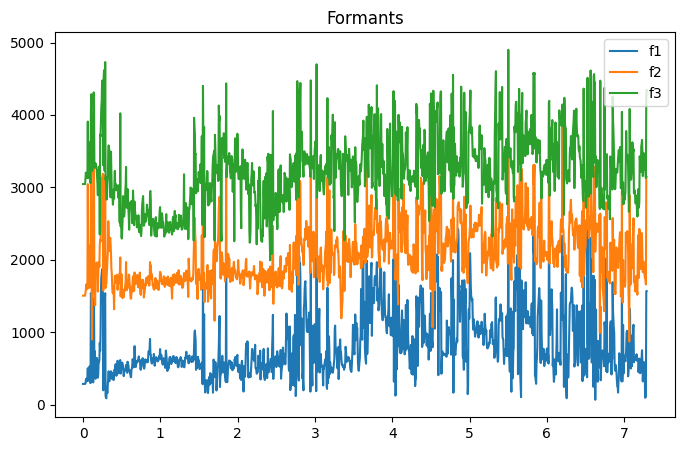
\includegraphics{03_TS_processing/02_TS_processing_acoustics_final_files/figure-pdf/cell-24-output-1.pdf}

Now let's look at the vowel space area across all data.

\includegraphics{03_TS_processing/02_TS_processing_acoustics_final_files/figure-pdf/cell-25-output-1.pdf}

And this is distribution of f1 across all data.

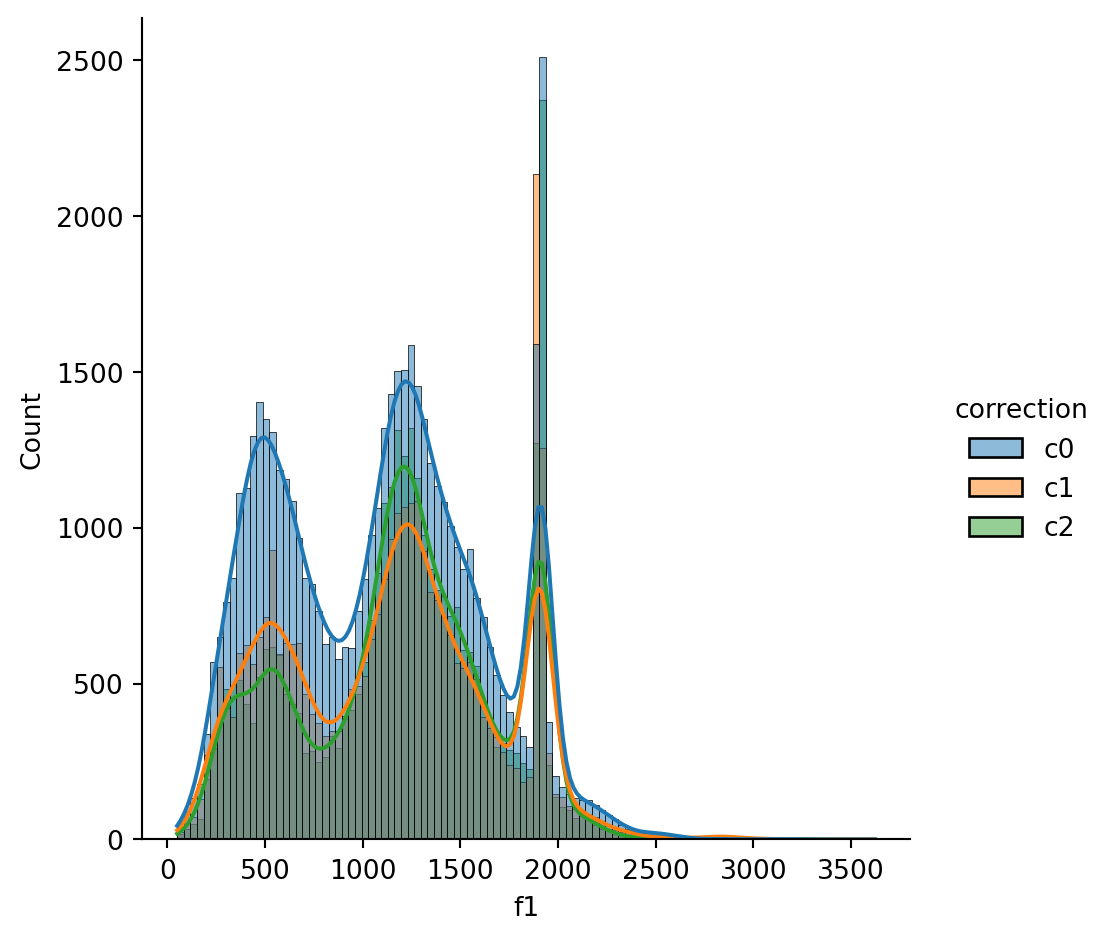
\includegraphics{03_TS_processing/02_TS_processing_acoustics_final_files/figure-pdf/cell-26-output-1.pdf}

This all looks reasonable. However, we should still be careful. Formant
values are most reliable where f0 is present. Since in this project, we
work with non-speech sounds, they are frequently unvoiced. Because
research shows that there are also formants beyond f0 contour
(REF-RAPH), we will also consider formant values in the moments of
envelope peaks. This will maximize the number of data points we can use
for analysis.

We can use \texttt{findpeaks()} function from the \texttt{signal}
package to find the peaks in the envelope. We can then use these peaks
as a reference point for formant extraction.

\begin{Shaded}
\begin{Highlighting}[]
\NormalTok{env\_df }\OperatorTok{=}\NormalTok{ pd.DataFrame()}

\CommentTok{\# loop over env files and make a giga df from all}
\ControlFlowTok{for}\NormalTok{ envfile }\KeywordTok{in}\NormalTok{ envfiles:}
\NormalTok{    df }\OperatorTok{=}\NormalTok{ pd.read\_csv(envfile)}
\NormalTok{    env\_df }\OperatorTok{=}\NormalTok{ pd.concat([env\_df, df])}
\end{Highlighting}
\end{Shaded}

Using \texttt{peak\_width} function, we can extract the window of an
envelope peak. Further, we can define the relative height of the peak to
adjust the window size. Here, we try relative height of 0.5 and 0.9

\begin{Shaded}
\begin{Highlighting}[]
\CommentTok{\# rename trialID to trialid}
\NormalTok{env\_df }\OperatorTok{=}\NormalTok{ env\_df.rename(columns}\OperatorTok{=}\NormalTok{\{}\StringTok{\textquotesingle{}trialID\textquotesingle{}}\NormalTok{: }\StringTok{\textquotesingle{}trialid\textquotesingle{}}\NormalTok{\})}

\CommentTok{\# pick a random trialid from env\_df}
\NormalTok{trialid }\OperatorTok{=} \StringTok{\textquotesingle{}0\_2\_62\_p1\textquotesingle{}}

\CommentTok{\# get the env for this trialid from env\_df}
\NormalTok{env\_trial }\OperatorTok{=}\NormalTok{ env\_df[env\_df[}\StringTok{\textquotesingle{}trialid\textquotesingle{}}\NormalTok{] }\OperatorTok{==}\NormalTok{ trialid]}

\CommentTok{\# find peaks, min height is mean of the env}
\NormalTok{peaks, \_ }\OperatorTok{=}\NormalTok{ find\_peaks(env\_trial[}\StringTok{\textquotesingle{}envelope\textquotesingle{}}\NormalTok{], height}\OperatorTok{=}\NormalTok{np.mean(env\_df[}\StringTok{\textquotesingle{}envelope\textquotesingle{}}\NormalTok{]))}

\CommentTok{\# get the width of the peaks}
\NormalTok{results\_half }\OperatorTok{=}\NormalTok{ peak\_widths(env\_trial[}\StringTok{\textquotesingle{}envelope\textquotesingle{}}\NormalTok{], peaks, rel\_height}\OperatorTok{=}\FloatTok{0.5}\NormalTok{)}
\NormalTok{results\_full }\OperatorTok{=}\NormalTok{ peak\_widths(env\_trial[}\StringTok{\textquotesingle{}envelope\textquotesingle{}}\NormalTok{], peaks, rel\_height}\OperatorTok{=}\FloatTok{0.9}\NormalTok{)}
\end{Highlighting}
\end{Shaded}

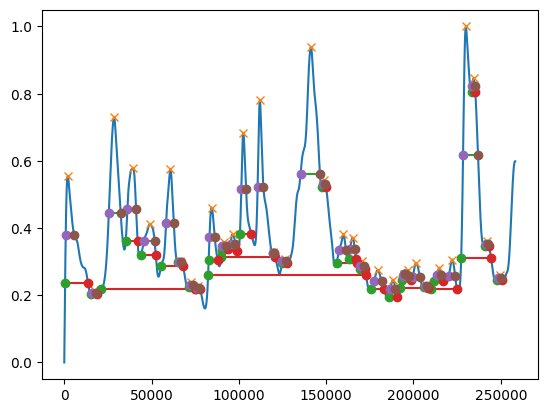
\includegraphics{03_TS_processing/02_TS_processing_acoustics_final_files/figure-pdf/cell-29-output-1.pdf}

Now we can check envelope peak widths against formant values. In merged
dataframe with both formants and envelope, we will annotate peak widths,
so that we know which values of formants to consider (the rest we turn
to NA)

\begin{Shaded}
\begin{Highlighting}[]
\CommentTok{\# find formants2 df with the same trialid}
\NormalTok{formants\_trial }\OperatorTok{=}\NormalTok{ formants\_df[formants\_df[}\StringTok{\textquotesingle{}trialid\textquotesingle{}}\NormalTok{] }\OperatorTok{==}\NormalTok{ trialid]}

\CommentTok{\# convert time to ms}
\NormalTok{formants\_trial[}\StringTok{\textquotesingle{}time\textquotesingle{}}\NormalTok{] }\OperatorTok{=}\NormalTok{ formants\_trial[}\StringTok{\textquotesingle{}time\textquotesingle{}}\NormalTok{] }\OperatorTok{*} \DecValTok{1000}

\CommentTok{\# merge formants1 and formants2 on trialid and time, outer method}
\NormalTok{merged\_df }\OperatorTok{=}\NormalTok{ pd.merge(env\_trial, formants\_trial, on}\OperatorTok{=}\NormalTok{[}\StringTok{\textquotesingle{}trialid\textquotesingle{}}\NormalTok{, }\StringTok{\textquotesingle{}time\textquotesingle{}}\NormalTok{], how}\OperatorTok{=}\StringTok{\textquotesingle{}outer\textquotesingle{}}\NormalTok{)}

\CommentTok{\# cols to int}
\NormalTok{colstoint }\OperatorTok{=}\NormalTok{ [}\StringTok{\textquotesingle{}f1\textquotesingle{}}\NormalTok{, }\StringTok{\textquotesingle{}f2\textquotesingle{}}\NormalTok{, }\StringTok{\textquotesingle{}f3\textquotesingle{}}\NormalTok{, }\StringTok{\textquotesingle{}f4\textquotesingle{}}\NormalTok{, }\StringTok{\textquotesingle{}f5\textquotesingle{}}\NormalTok{]}

\CommentTok{\#interpolate }
\ControlFlowTok{for}\NormalTok{ col }\KeywordTok{in}\NormalTok{ colstoint:}
\NormalTok{    merged\_df[col] }\OperatorTok{=}\NormalTok{ merged\_df[col].interpolate(method}\OperatorTok{=}\StringTok{\textquotesingle{}linear\textquotesingle{}}\NormalTok{, x }\OperatorTok{=}\NormalTok{ merged\_df[}\StringTok{\textquotesingle{}time\textquotesingle{}}\NormalTok{])}

\CommentTok{\#delete rows where envelope is NaN}
\NormalTok{merged\_df }\OperatorTok{=}\NormalTok{ merged\_df.dropna(subset}\OperatorTok{=}\NormalTok{[}\StringTok{\textquotesingle{}envelope\textquotesingle{}}\NormalTok{])}

\CommentTok{\# check the width of the peaks}
\NormalTok{peaks, \_ }\OperatorTok{=}\NormalTok{ find\_peaks(merged\_df[}\StringTok{\textquotesingle{}envelope\textquotesingle{}}\NormalTok{], height}\OperatorTok{=}\NormalTok{np.mean(env\_df[}\StringTok{\textquotesingle{}envelope\textquotesingle{}}\NormalTok{])) }\CommentTok{\# minimum height of the peak is mean of the envelope (across all data)}

\CommentTok{\# get the width of the peaks}
\NormalTok{results\_width }\OperatorTok{=}\NormalTok{ peak\_widths(merged\_df[}\StringTok{\textquotesingle{}envelope\textquotesingle{}}\NormalTok{], peaks, rel\_height}\OperatorTok{=}\FloatTok{0.9}\NormalTok{)}

\CommentTok{\# create column peak\_width and put 1 everywhere between start and end of the peak}
\NormalTok{merged\_df[}\StringTok{\textquotesingle{}peak\_width\textquotesingle{}}\NormalTok{] }\OperatorTok{=} \DecValTok{0}

\CommentTok{\# create a table from the results\_half[2] and results\_half[3]}
\NormalTok{peak\_w }\OperatorTok{=}\NormalTok{ pd.DataFrame(\{}\StringTok{\textquotesingle{}start\textquotesingle{}}\NormalTok{: results\_width[}\DecValTok{2}\NormalTok{], }\StringTok{\textquotesingle{}end\textquotesingle{}}\NormalTok{: results\_width[}\DecValTok{3}\NormalTok{]\})}

\CommentTok{\# loop over the rows of the peak\_w and put 1 in the peak\_width column between start and end}
\ControlFlowTok{for}\NormalTok{ i, row }\KeywordTok{in}\NormalTok{ peak\_w.iterrows():}
\NormalTok{    merged\_df.loc[row[}\StringTok{\textquotesingle{}start\textquotesingle{}}\NormalTok{]:row[}\StringTok{\textquotesingle{}end\textquotesingle{}}\NormalTok{], }\StringTok{\textquotesingle{}peak\_width\textquotesingle{}}\NormalTok{] }\OperatorTok{=} \DecValTok{1}

\CommentTok{\# for each formant column, create new f\_clean column and put the value of the formant where peak\_width = 1}
\ControlFlowTok{for}\NormalTok{ col }\KeywordTok{in}\NormalTok{ colstoint:}
\NormalTok{    merged\_df[col }\OperatorTok{+} \StringTok{\textquotesingle{}\_clean\textquotesingle{}}\NormalTok{] }\OperatorTok{=}\NormalTok{ merged\_df[col] }\OperatorTok{*}\NormalTok{ merged\_df[}\StringTok{\textquotesingle{}peak\_width\textquotesingle{}}\NormalTok{]}
    \CommentTok{\#instead of 0, put NaN}
\NormalTok{    merged\_df[col }\OperatorTok{+} \StringTok{\textquotesingle{}\_clean\textquotesingle{}}\NormalTok{] }\OperatorTok{=}\NormalTok{ merged\_df[col }\OperatorTok{+} \StringTok{\textquotesingle{}\_clean\textquotesingle{}}\NormalTok{].replace(}\DecValTok{0}\NormalTok{, np.nan)}
\end{Highlighting}
\end{Shaded}

Here we can see visualized overlap of formants and envelope (peaks). The
darker part of the formants signal is the window of an envelope peak.

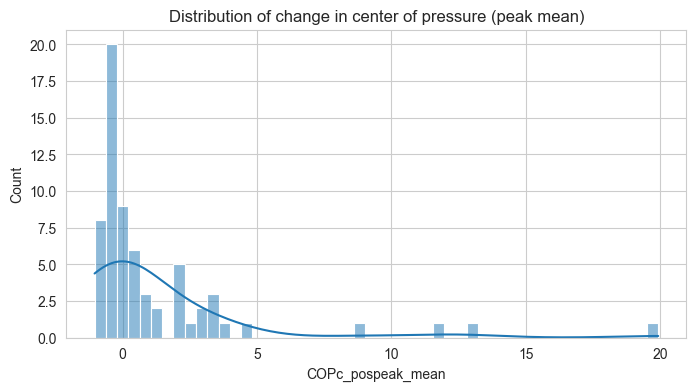
\includegraphics{03_TS_processing/02_TS_processing_acoustics_final_files/figure-pdf/cell-31-output-1.pdf}

In script (\textbf{ADD?}), we will get back to this and use both
envelope peaks and f0 to define the relevant formant windows.

\bookmarksetup{startatroot}

\chapter{Processing III: Merging multimodal
data}\label{processing-iii-merging-multimodal-data}

In the previous scripts, we have preprocessed various motion and
acoustic data. In this script, we will merge the data into a single file
per trial. These data include:

\begin{itemize}
\tightlist
\item
  Balance Board data
\item
  Kinematics
\item
  Joint angles
\item
  Joint moments
\item
  Amplitude envelope
\item
  f0
\item
  Formants
\item
  Spectral centroid
\end{itemize}

\begin{Shaded}
\begin{Highlighting}[]
\CommentTok{\# packages}
\ImportTok{import}\NormalTok{ os}
\ImportTok{import}\NormalTok{ glob}
\ImportTok{import}\NormalTok{ numpy }\ImportTok{as}\NormalTok{ np}
\ImportTok{import}\NormalTok{ pandas }\ImportTok{as}\NormalTok{ pd}
\ImportTok{import}\NormalTok{ matplotlib.pyplot }\ImportTok{as}\NormalTok{ plt}
\ImportTok{import}\NormalTok{ scipy}
\ImportTok{import}\NormalTok{ matplotlib.pyplot }\ImportTok{as}\NormalTok{ plt}
\ImportTok{import}\NormalTok{ seaborn }\ImportTok{as}\NormalTok{ sns}

\NormalTok{curfolder }\OperatorTok{=}\NormalTok{ os.getcwd()}

\CommentTok{\# folders with processed data}
\NormalTok{MTfolder\_processed }\OperatorTok{=}\NormalTok{ curfolder }\OperatorTok{+} \StringTok{\textquotesingle{}}\CharTok{\textbackslash{}\textbackslash{}}\StringTok{TS\_motiontracking}\CharTok{\textbackslash{}\textbackslash{}}\StringTok{\textquotesingle{}}
\NormalTok{ACfolder\_processed }\OperatorTok{=}\NormalTok{ curfolder }\OperatorTok{+} \StringTok{\textquotesingle{}}\CharTok{\textbackslash{}\textbackslash{}}\StringTok{TS\_acoustics}\CharTok{\textbackslash{}\textbackslash{}}\StringTok{\textquotesingle{}}
\CommentTok{\# folder to save merged data}
\NormalTok{TSmerged }\OperatorTok{=}\NormalTok{ curfolder }\OperatorTok{+} \StringTok{\textquotesingle{}}\CharTok{\textbackslash{}\textbackslash{}}\StringTok{TS\_merged}\CharTok{\textbackslash{}\textbackslash{}}\StringTok{\textquotesingle{}}

\CommentTok{\# prepare all files}
\NormalTok{bbfiles }\OperatorTok{=}\NormalTok{ glob.glob(MTfolder\_processed }\OperatorTok{+} \StringTok{\textquotesingle{}/bb*.csv\textquotesingle{}}\NormalTok{)}
\NormalTok{idfiles }\OperatorTok{=}\NormalTok{ glob.glob(MTfolder\_processed }\OperatorTok{+} \StringTok{\textquotesingle{}/id*.csv\textquotesingle{}}\NormalTok{)}
\NormalTok{ikfiles }\OperatorTok{=}\NormalTok{ glob.glob(MTfolder\_processed }\OperatorTok{+} \StringTok{\textquotesingle{}/ik*.csv\textquotesingle{}}\NormalTok{)}
\NormalTok{mtfiles }\OperatorTok{=}\NormalTok{ glob.glob(MTfolder\_processed }\OperatorTok{+} \StringTok{\textquotesingle{}/mt*.csv\textquotesingle{}}\NormalTok{)}
\NormalTok{envfiles }\OperatorTok{=}\NormalTok{ glob.glob(ACfolder\_processed }\OperatorTok{+} \StringTok{\textquotesingle{}/env*.csv\textquotesingle{}}\NormalTok{)}
\NormalTok{f0files }\OperatorTok{=}\NormalTok{ glob.glob(ACfolder\_processed }\OperatorTok{+} \StringTok{\textquotesingle{}/f0*.csv\textquotesingle{}}\NormalTok{)}
\NormalTok{formants }\OperatorTok{=}\NormalTok{ glob.glob(ACfolder\_processed }\OperatorTok{+} \StringTok{\textquotesingle{}/praat\_formants*.csv\textquotesingle{}}\NormalTok{)}
\NormalTok{scfiles }\OperatorTok{=}\NormalTok{ glob.glob(ACfolder\_processed }\OperatorTok{+} \StringTok{\textquotesingle{}/cog*.csv\textquotesingle{}}\NormalTok{)}
\end{Highlighting}
\end{Shaded}

When extracting and processing the signals in scripts
(\textbf{ADDREF?}), we kept the sampling rates untouched. This means
that now we have a variety of timeseries that each samples at different
frequency. Inspecting a trial per each signal, we see the following
sampling rates:

\begin{verbatim}
balance board: 499.986924434759
inverse dynamics: 60.00535247744097
inverse kinematics: 59.999988000002396
kinematics: 60.00000000000024
envelope: 48000.00000000008
f0: 487.16350507461976
formants: 38415.36614645814
spectral centroid: 472.65436024146993
\end{verbatim}

We opt for 500 Hz as the final sampling rate we will merge on. That
means that we will interpolate all missing data (using linear
interpolation) to match this frequency.

Additionally, we will adapt the formants such that we only consider
values that are present within a range of an amplitude peak (see
(\textbf{ADDREF?}) for more details), or where f0 is present, or both.
These two situations can be considered as yielding in the most reliable
formant values.

Finally, we will also use inverse kinematics and dynamics to calculate
power (as joint moment × joint velocity) and smooth it with
1st-polynomial Savitzky-Golay filter with span of 560 ms.

\begin{Shaded}
\begin{Highlighting}[]
\CommentTok{\# Function to create chunks of non{-}NaN values in a dataframe}
\KeywordTok{def}\NormalTok{ create\_chunks(df, var):}

\NormalTok{    df[}\StringTok{\textquotesingle{}chunk\textquotesingle{}}\NormalTok{] }\OperatorTok{=} \VariableTok{None}

    \CommentTok{\# annotate chunks of non{-}NaN values}
\NormalTok{    chunk }\OperatorTok{=} \DecValTok{0}
    \ControlFlowTok{for}\NormalTok{ index, row }\KeywordTok{in}\NormalTok{ df.iterrows():}
        \ControlFlowTok{if}\NormalTok{ np.isnan(row[var]):}
            \ControlFlowTok{continue}
        \ControlFlowTok{else}\NormalTok{:}
\NormalTok{            df.loc[index, }\StringTok{\textquotesingle{}chunk\textquotesingle{}}\NormalTok{] }\OperatorTok{=}\NormalTok{ chunk}
            \CommentTok{\# if the next value is NaN or this is the last row, increase the chunk}
            \ControlFlowTok{if}\NormalTok{ index }\OperatorTok{==} \BuiltInTok{len}\NormalTok{(df)}\OperatorTok{{-}}\DecValTok{1}\NormalTok{:}
                \ControlFlowTok{continue}
            \ControlFlowTok{elif}\NormalTok{ np.isnan(df.loc[index}\OperatorTok{+}\DecValTok{1}\NormalTok{, var]):}
\NormalTok{                chunk }\OperatorTok{+=} \DecValTok{1}

\NormalTok{    chunks }\OperatorTok{=}\NormalTok{ df[}\StringTok{\textquotesingle{}chunk\textquotesingle{}}\NormalTok{].unique()}

    \ControlFlowTok{if} \BuiltInTok{len}\NormalTok{(chunks) }\OperatorTok{\textgreater{}} \DecValTok{1}\NormalTok{: }\CommentTok{\# skip if chunks are empty (that means that there is no f0 trace)}
        \CommentTok{\# ignore the first chunk (None)}
\NormalTok{        chunks }\OperatorTok{=}\NormalTok{ chunks[}\DecValTok{1}\NormalTok{:]}

    \ControlFlowTok{return}\NormalTok{ df, chunks}

\CommentTok{\# Function to interpolate chunks of non{-}NaN values in a dataframe to maintain discontinuities in the signal}
\KeywordTok{def}\NormalTok{ interpolate\_chunks(df, chunks, var):}
    \CommentTok{\# we ignore the None chunk above, so if there is some trace, None should not be within chunks}
    \ControlFlowTok{if} \VariableTok{None} \KeywordTok{not} \KeywordTok{in}\NormalTok{ chunks:}
        \ControlFlowTok{for}\NormalTok{ chunk }\KeywordTok{in}\NormalTok{ chunks:}
            \CommentTok{\# get the first and last row of the chunk}
\NormalTok{            firstrow }\OperatorTok{=}\NormalTok{ df[df[}\StringTok{\textquotesingle{}chunk\textquotesingle{}}\NormalTok{] }\OperatorTok{==}\NormalTok{ chunk].index[}\DecValTok{0}\NormalTok{]}
\NormalTok{            lastrow }\OperatorTok{=}\NormalTok{ df[df[}\StringTok{\textquotesingle{}chunk\textquotesingle{}}\NormalTok{] }\OperatorTok{==}\NormalTok{ chunk].index[}\OperatorTok{{-}}\DecValTok{1}\NormalTok{]}
            \CommentTok{\# fill all inbetween with the chunk number}
\NormalTok{            df.loc[firstrow:lastrow, }\StringTok{\textquotesingle{}chunk\textquotesingle{}}\NormalTok{] }\OperatorTok{=}\NormalTok{ chunk}
            \CommentTok{\# get the rows of the chunk}
\NormalTok{            chunkrows }\OperatorTok{=}\NormalTok{ df[df[}\StringTok{\textquotesingle{}chunk\textquotesingle{}}\NormalTok{] }\OperatorTok{==}\NormalTok{ chunk].copy()}
            \CommentTok{\# interpolate}
\NormalTok{            chunkrows[var] }\OperatorTok{=}\NormalTok{ chunkrows[var].interpolate(method}\OperatorTok{=}\StringTok{\textquotesingle{}linear\textquotesingle{}}\NormalTok{, x }\OperatorTok{=}\NormalTok{ chunkrows[}\StringTok{\textquotesingle{}time\textquotesingle{}}\NormalTok{])}
            \CommentTok{\# put the interpolated chunk back to the df}
\NormalTok{            df.loc[df[}\StringTok{\textquotesingle{}chunk\textquotesingle{}}\NormalTok{] }\OperatorTok{==}\NormalTok{ chunk, var] }\OperatorTok{=}\NormalTok{ chunkrows[var]}

    \CommentTok{\# get rid of the chunk column}
\NormalTok{    df.drop(}\StringTok{\textquotesingle{}chunk\textquotesingle{}}\NormalTok{, axis}\OperatorTok{=}\DecValTok{1}\NormalTok{, inplace}\OperatorTok{=}\VariableTok{True}\NormalTok{)}

    \ControlFlowTok{return}\NormalTok{ df}
\end{Highlighting}
\end{Shaded}

\begin{Shaded}
\begin{Highlighting}[]
\NormalTok{desired\_sr }\OperatorTok{=} \FloatTok{0.5}    \CommentTok{\# this is the sr we are going to merge on (in Hz/sec)}

\NormalTok{error\_log }\OperatorTok{=}\NormalTok{ []}

\ControlFlowTok{for} \BuiltInTok{file} \KeywordTok{in}\NormalTok{ bbfiles:}

\NormalTok{    bb\_df }\OperatorTok{=}\NormalTok{ pd.read\_csv(}\BuiltInTok{file}\NormalTok{)}
    \CommentTok{\# get trial id}
\NormalTok{    trialid }\OperatorTok{=}\NormalTok{ bb\_df[}\StringTok{\textquotesingle{}TrialID\textquotesingle{}}\NormalTok{][}\DecValTok{0}\NormalTok{]}

    \BuiltInTok{print}\NormalTok{(}\StringTok{\textquotesingle{}working on \textquotesingle{}} \OperatorTok{+}\NormalTok{ trialid)}
    
    \CommentTok{\# find the same trialid in idfiles}
\NormalTok{    id\_file }\OperatorTok{=}\NormalTok{ [x }\ControlFlowTok{for}\NormalTok{ x }\KeywordTok{in}\NormalTok{ idfiles }\ControlFlowTok{if}\NormalTok{ trialid }\KeywordTok{in}\NormalTok{ x]}
    \ControlFlowTok{try}\NormalTok{:}
\NormalTok{        id\_df }\OperatorTok{=}\NormalTok{ pd.read\_csv(id\_file[}\DecValTok{0}\NormalTok{])}
    \ControlFlowTok{except} \PreprocessorTok{IndexError}\NormalTok{:}
        \BuiltInTok{print}\NormalTok{(}\StringTok{\textquotesingle{}IndexError: \textquotesingle{}} \OperatorTok{+}\NormalTok{ trialid }\OperatorTok{+} \StringTok{\textquotesingle{} not found\textquotesingle{}}\NormalTok{)}
\NormalTok{        errormessage }\OperatorTok{=} \StringTok{\textquotesingle{}IndexError: \textquotesingle{}} \OperatorTok{+}\NormalTok{ trialid }\OperatorTok{+} \StringTok{\textquotesingle{} not found for ID\textquotesingle{}}
\NormalTok{        error\_log.append(errormessage)}
        \ControlFlowTok{continue}
    
    \CommentTok{\# find the same trialid in mtfiles}
\NormalTok{    mt\_file }\OperatorTok{=}\NormalTok{ [x }\ControlFlowTok{for}\NormalTok{ x }\KeywordTok{in}\NormalTok{ mtfiles }\ControlFlowTok{if}\NormalTok{ trialid }\KeywordTok{in}\NormalTok{ x]}
    \ControlFlowTok{try}\NormalTok{:}
\NormalTok{        mt\_df }\OperatorTok{=}\NormalTok{ pd.read\_csv(mt\_file[}\DecValTok{0}\NormalTok{])}
    \ControlFlowTok{except} \PreprocessorTok{IndexError}\NormalTok{:}
        \BuiltInTok{print}\NormalTok{(}\StringTok{\textquotesingle{}IndexError: \textquotesingle{}} \OperatorTok{+}\NormalTok{ trialid }\OperatorTok{+} \StringTok{\textquotesingle{} not found\textquotesingle{}}\NormalTok{)}
\NormalTok{        errormessage }\OperatorTok{=} \StringTok{\textquotesingle{}IndexError: \textquotesingle{}} \OperatorTok{+}\NormalTok{ trialid }\OperatorTok{+} \StringTok{\textquotesingle{} not found for MT\textquotesingle{}}
\NormalTok{        error\_log.append(errormessage)}
        \ControlFlowTok{continue}
    \CommentTok{\# rename Time to time}
\NormalTok{    mt\_df.rename(columns}\OperatorTok{=}\NormalTok{\{}\StringTok{\textquotesingle{}Time\textquotesingle{}}\NormalTok{: }\StringTok{\textquotesingle{}time\textquotesingle{}}\NormalTok{\}, inplace}\OperatorTok{=}\VariableTok{True}\NormalTok{)}

    \CommentTok{\# find the same trialid in envfiles}
\NormalTok{    env\_file }\OperatorTok{=}\NormalTok{ [x }\ControlFlowTok{for}\NormalTok{ x }\KeywordTok{in}\NormalTok{ envfiles }\ControlFlowTok{if}\NormalTok{ trialid }\KeywordTok{in}\NormalTok{ x]}
    \ControlFlowTok{try}\NormalTok{:}
\NormalTok{        env\_df }\OperatorTok{=}\NormalTok{ pd.read\_csv(env\_file[}\DecValTok{0}\NormalTok{])}
    \ControlFlowTok{except} \PreprocessorTok{IndexError}\NormalTok{:}
        \BuiltInTok{print}\NormalTok{(}\StringTok{\textquotesingle{}IndexError: \textquotesingle{}} \OperatorTok{+}\NormalTok{ trialid }\OperatorTok{+} \StringTok{\textquotesingle{} not found\textquotesingle{}}\NormalTok{)}
\NormalTok{        errormessage }\OperatorTok{=} \StringTok{\textquotesingle{}IndexError: \textquotesingle{}} \OperatorTok{+}\NormalTok{ trialid }\OperatorTok{+} \StringTok{\textquotesingle{} not found for ENV\textquotesingle{}}
\NormalTok{        error\_log.append(errormessage)}
        \ControlFlowTok{continue}
    
    \CommentTok{\# rename trialID to TrialID}
\NormalTok{    env\_df.rename(columns}\OperatorTok{=}\NormalTok{\{}\StringTok{\textquotesingle{}trialID\textquotesingle{}}\NormalTok{: }\StringTok{\textquotesingle{}TrialID\textquotesingle{}}\NormalTok{\}, inplace}\OperatorTok{=}\VariableTok{True}\NormalTok{)}

    \CommentTok{\# find the same trialid in f0files}
\NormalTok{    f0\_file }\OperatorTok{=}\NormalTok{ [x }\ControlFlowTok{for}\NormalTok{ x }\KeywordTok{in}\NormalTok{ f0files }\ControlFlowTok{if}\NormalTok{ trialid }\KeywordTok{in}\NormalTok{ x]}
    \ControlFlowTok{try}\NormalTok{:}
\NormalTok{        f0\_df }\OperatorTok{=}\NormalTok{ pd.read\_csv(f0\_file[}\DecValTok{0}\NormalTok{])}
    \ControlFlowTok{except} \PreprocessorTok{IndexError}\NormalTok{:}
        \BuiltInTok{print}\NormalTok{(}\StringTok{\textquotesingle{}IndexError: \textquotesingle{}} \OperatorTok{+}\NormalTok{ trialid }\OperatorTok{+} \StringTok{\textquotesingle{} not found\textquotesingle{}}\NormalTok{)}
\NormalTok{        errormessage }\OperatorTok{=} \StringTok{\textquotesingle{}IndexError: \textquotesingle{}} \OperatorTok{+}\NormalTok{ trialid }\OperatorTok{+} \StringTok{\textquotesingle{} not found for F0\textquotesingle{}}
\NormalTok{        error\_log.append(errormessage)}
        \ControlFlowTok{continue}

    \CommentTok{\# rename time\_ms to time}
\NormalTok{    f0\_df.rename(columns}\OperatorTok{=}\NormalTok{\{}\StringTok{\textquotesingle{}time\_ms\textquotesingle{}}\NormalTok{: }\StringTok{\textquotesingle{}time\textquotesingle{}}\NormalTok{\}, inplace}\OperatorTok{=}\VariableTok{True}\NormalTok{)}
    \CommentTok{\# rename ID to TrialID}
\NormalTok{    f0\_df.rename(columns}\OperatorTok{=}\NormalTok{\{}\StringTok{\textquotesingle{}ID\textquotesingle{}}\NormalTok{: }\StringTok{\textquotesingle{}TrialID\textquotesingle{}}\NormalTok{\}, inplace}\OperatorTok{=}\VariableTok{True}\NormalTok{)}

    \CommentTok{\# find the same trialid in ikfiles}
\NormalTok{    ik\_file }\OperatorTok{=}\NormalTok{ [x }\ControlFlowTok{for}\NormalTok{ x }\KeywordTok{in}\NormalTok{ ikfiles }\ControlFlowTok{if}\NormalTok{ trialid }\KeywordTok{in}\NormalTok{ x]}
    \ControlFlowTok{try}\NormalTok{:}
\NormalTok{        ik\_df }\OperatorTok{=}\NormalTok{ pd.read\_csv(ik\_file[}\DecValTok{0}\NormalTok{])}
    \ControlFlowTok{except} \PreprocessorTok{IndexError}\NormalTok{:}
        \BuiltInTok{print}\NormalTok{(}\StringTok{\textquotesingle{}IndexError: \textquotesingle{}} \OperatorTok{+}\NormalTok{ trialid }\OperatorTok{+} \StringTok{\textquotesingle{} not found\textquotesingle{}}\NormalTok{)}
\NormalTok{        errormessage }\OperatorTok{=} \StringTok{\textquotesingle{}IndexError: \textquotesingle{}} \OperatorTok{+}\NormalTok{ trialid }\OperatorTok{+} \StringTok{\textquotesingle{} not found for IK\textquotesingle{}}
\NormalTok{        error\_log.append(errormessage)}
        \ControlFlowTok{continue}

    \CommentTok{\# find the same trialid in formants}
\NormalTok{    formants\_file }\OperatorTok{=}\NormalTok{ [x }\ControlFlowTok{for}\NormalTok{ x }\KeywordTok{in}\NormalTok{ formants }\ControlFlowTok{if}\NormalTok{ trialid }\KeywordTok{in}\NormalTok{ x]}
    \ControlFlowTok{try}\NormalTok{:}
\NormalTok{        formants\_df }\OperatorTok{=}\NormalTok{ pd.read\_csv(formants\_file[}\DecValTok{0}\NormalTok{])}
    \ControlFlowTok{except} \PreprocessorTok{IndexError}\NormalTok{:}
        \BuiltInTok{print}\NormalTok{(}\StringTok{\textquotesingle{}IndexError: \textquotesingle{}} \OperatorTok{+}\NormalTok{ trialid }\OperatorTok{+} \StringTok{\textquotesingle{}not found\textquotesingle{}}\NormalTok{)}
\NormalTok{        errormessage }\OperatorTok{=} \StringTok{\textquotesingle{}IndexError: \textquotesingle{}} \OperatorTok{+}\NormalTok{ trialid }\OperatorTok{+} \StringTok{\textquotesingle{} not found for formants\textquotesingle{}}
\NormalTok{        error\_log.append(errormessage)}
        \ControlFlowTok{continue}

    \CommentTok{\# rename triald to TrialID}
\NormalTok{    formants\_df.rename(columns}\OperatorTok{=}\NormalTok{\{}\StringTok{\textquotesingle{}trialid\textquotesingle{}}\NormalTok{: }\StringTok{\textquotesingle{}TrialID\textquotesingle{}}\NormalTok{\}, inplace}\OperatorTok{=}\VariableTok{True}\NormalTok{)}
\NormalTok{    formants\_df }\OperatorTok{=}\NormalTok{ formants\_df[[}\StringTok{\textquotesingle{}time\textquotesingle{}}\NormalTok{, }\StringTok{\textquotesingle{}f1\textquotesingle{}}\NormalTok{, }\StringTok{\textquotesingle{}f2\textquotesingle{}}\NormalTok{, }\StringTok{\textquotesingle{}f3\textquotesingle{}}\NormalTok{, }\StringTok{\textquotesingle{}TrialID\textquotesingle{}}\NormalTok{]]}
\NormalTok{    formants\_df[}\StringTok{\textquotesingle{}time\textquotesingle{}}\NormalTok{] }\OperatorTok{=}\NormalTok{ formants\_df[}\StringTok{\textquotesingle{}time\textquotesingle{}}\NormalTok{] }\OperatorTok{*} \DecValTok{1000}

    \CommentTok{\# find the same triaalid in CoG}
\NormalTok{    sc\_file }\OperatorTok{=}\NormalTok{ [x }\ControlFlowTok{for}\NormalTok{ x }\KeywordTok{in}\NormalTok{ scfiles }\ControlFlowTok{if}\NormalTok{ trialid }\KeywordTok{in}\NormalTok{ x]}
    \ControlFlowTok{try}\NormalTok{:}
\NormalTok{        sc\_df }\OperatorTok{=}\NormalTok{ pd.read\_csv(sc\_file[}\DecValTok{0}\NormalTok{])}
    \ControlFlowTok{except} \PreprocessorTok{IndexError}\NormalTok{:}
        \BuiltInTok{print}\NormalTok{(}\StringTok{\textquotesingle{}IndexError: \textquotesingle{}} \OperatorTok{+}\NormalTok{ trialid }\OperatorTok{+} \StringTok{\textquotesingle{}not found\textquotesingle{}}\NormalTok{)}
\NormalTok{        errormessage }\OperatorTok{=} \StringTok{\textquotesingle{}IndexError: \textquotesingle{}} \OperatorTok{+}\NormalTok{ trialid }\OperatorTok{+} \StringTok{\textquotesingle{} not found for CoG\textquotesingle{}}
\NormalTok{        error\_log.append(errormessage)}
        \ControlFlowTok{continue}

    \CommentTok{\# write error log}
    \ControlFlowTok{with} \BuiltInTok{open}\NormalTok{(TSmerged }\OperatorTok{+} \StringTok{\textquotesingle{}/error\_log.txt\textquotesingle{}}\NormalTok{, }\StringTok{\textquotesingle{}w\textquotesingle{}}\NormalTok{) }\ImportTok{as}\NormalTok{ f:}
        \ControlFlowTok{for}\NormalTok{ item }\KeywordTok{in}\NormalTok{ error\_log:}
\NormalTok{            f.write(}\StringTok{"}\SpecialCharTok{\%s}\CharTok{\textbackslash{}n}\StringTok{"} \OperatorTok{\%}\NormalTok{ item)}


    \CommentTok{\#\#\#\#\#\#\#\#\#\#\#\#\#\# MERGING \#\#\#\#\#\#\#\#\#\#\#\#\#\#\#\#\#\#\#\#\#\#\#\#}

    \CommentTok{\#\#\#\# regularize sr in bb}
\NormalTok{    time\_new }\OperatorTok{=}\NormalTok{ np.arange(}\DecValTok{0}\NormalTok{, }\BuiltInTok{max}\NormalTok{(bb\_df[}\StringTok{\textquotesingle{}time\textquotesingle{}}\NormalTok{]), }\DecValTok{1}\OperatorTok{/}\NormalTok{desired\_sr)}
\NormalTok{    bb\_interp }\OperatorTok{=}\NormalTok{ pd.DataFrame(\{}\StringTok{\textquotesingle{}time\textquotesingle{}}\NormalTok{: time\_new\})}
    
    \CommentTok{\# interpolate all columns in samplebb }
\NormalTok{    colstoint }\OperatorTok{=}\NormalTok{ bb\_df.columns}
\NormalTok{    colstoint }\OperatorTok{=}\NormalTok{ [x }\ControlFlowTok{for}\NormalTok{ x }\KeywordTok{in}\NormalTok{ colstoint }\ControlFlowTok{if} \StringTok{\textquotesingle{}time\textquotesingle{}} \KeywordTok{not} \KeywordTok{in}\NormalTok{ x]}
\NormalTok{    colstoint }\OperatorTok{=}\NormalTok{ [x }\ControlFlowTok{for}\NormalTok{ x }\KeywordTok{in}\NormalTok{ colstoint }\ControlFlowTok{if} \StringTok{\textquotesingle{}TrialID\textquotesingle{}} \KeywordTok{not} \KeywordTok{in}\NormalTok{ x]}
\NormalTok{    colstoint }\OperatorTok{=}\NormalTok{ [x }\ControlFlowTok{for}\NormalTok{ x }\KeywordTok{in}\NormalTok{ colstoint }\ControlFlowTok{if} \StringTok{\textquotesingle{}FileInfo\textquotesingle{}} \KeywordTok{not} \KeywordTok{in}\NormalTok{ x]}

    \ControlFlowTok{for}\NormalTok{ col }\KeywordTok{in}\NormalTok{ colstoint:}
\NormalTok{        bb\_interp[col] }\OperatorTok{=}\NormalTok{ bb\_df[col].interpolate(method}\OperatorTok{=}\StringTok{\textquotesingle{}linear\textquotesingle{}}\NormalTok{, x }\OperatorTok{=}\NormalTok{ bb\_interp[}\StringTok{\textquotesingle{}time\textquotesingle{}}\NormalTok{])}

    \CommentTok{\# add trialid and time}
\NormalTok{    bb\_interp[}\StringTok{\textquotesingle{}TrialID\textquotesingle{}}\NormalTok{] }\OperatorTok{=}\NormalTok{ trialid}
\NormalTok{    bb\_interp[}\StringTok{\textquotesingle{}FileInfo\textquotesingle{}}\NormalTok{] }\OperatorTok{=}\NormalTok{ bb\_df[}\StringTok{\textquotesingle{}FileInfo\textquotesingle{}}\NormalTok{][}\DecValTok{0}\NormalTok{]}
    
    \CommentTok{\#\#\#\#\#\#\#\#\#\#\# merge the bb\_interp with env}
    \CommentTok{\# merge the two dataframes}
\NormalTok{    merge1 }\OperatorTok{=}\NormalTok{ pd.merge(bb\_interp, env\_df, on}\OperatorTok{=}\NormalTok{[}\StringTok{\textquotesingle{}time\textquotesingle{}}\NormalTok{, }\StringTok{\textquotesingle{}TrialID\textquotesingle{}}\NormalTok{], how}\OperatorTok{=}\StringTok{\textquotesingle{}outer\textquotesingle{}}\NormalTok{)}

    \CommentTok{\# interpolate missing values of envelope and audio}
\NormalTok{    colstoint }\OperatorTok{=}\NormalTok{ merge1.columns}
\NormalTok{    colstoint }\OperatorTok{=}\NormalTok{ [x }\ControlFlowTok{for}\NormalTok{ x }\KeywordTok{in}\NormalTok{ colstoint }\ControlFlowTok{if} \StringTok{\textquotesingle{}audio\textquotesingle{}} \KeywordTok{in}\NormalTok{ x }\KeywordTok{or} \StringTok{\textquotesingle{}envelope\textquotesingle{}} \KeywordTok{in}\NormalTok{ x]}

    \ControlFlowTok{for}\NormalTok{ col }\KeywordTok{in}\NormalTok{ colstoint: }
\NormalTok{        merge1[col] }\OperatorTok{=}\NormalTok{ merge1[col].interpolate(method}\OperatorTok{=}\StringTok{\textquotesingle{}linear\textquotesingle{}}\NormalTok{, x }\OperatorTok{=}\NormalTok{ merge1[}\StringTok{\textquotesingle{}time\textquotesingle{}}\NormalTok{])}

    \CommentTok{\# now we can kick out all values where COPc is NaN}
\NormalTok{    merge1 }\OperatorTok{=}\NormalTok{ merge1[}\OperatorTok{\textasciitilde{}}\NormalTok{np.isnan(merge1[}\StringTok{\textquotesingle{}COPc\textquotesingle{}}\NormalTok{])]}

    \CommentTok{\#\#\#\#\#\#\#\#\#\#\# merge with ID}
    \CommentTok{\# merge the two dataframes}
\NormalTok{    merge2 }\OperatorTok{=}\NormalTok{ pd.merge(merge1, id\_df, on}\OperatorTok{=}\NormalTok{[}\StringTok{\textquotesingle{}time\textquotesingle{}}\NormalTok{, }\StringTok{\textquotesingle{}TrialID\textquotesingle{}}\NormalTok{], how}\OperatorTok{=}\StringTok{\textquotesingle{}outer\textquotesingle{}}\NormalTok{)}

    \CommentTok{\# get cols of sampleid}
\NormalTok{    colstoint }\OperatorTok{=}\NormalTok{ id\_df.columns}
\NormalTok{    colstoint }\OperatorTok{=}\NormalTok{ [x }\ControlFlowTok{for}\NormalTok{ x }\KeywordTok{in}\NormalTok{ colstoint }\ControlFlowTok{if} \StringTok{\textquotesingle{}time\textquotesingle{}} \KeywordTok{not} \KeywordTok{in}\NormalTok{ x]}
\NormalTok{    colstoint }\OperatorTok{=}\NormalTok{ [x }\ControlFlowTok{for}\NormalTok{ x }\KeywordTok{in}\NormalTok{ colstoint }\ControlFlowTok{if} \StringTok{\textquotesingle{}TrialID\textquotesingle{}} \KeywordTok{not} \KeywordTok{in}\NormalTok{ x]}

    \CommentTok{\# interpolate }
    \ControlFlowTok{for}\NormalTok{ col }\KeywordTok{in}\NormalTok{ colstoint:}
\NormalTok{        merge2[col] }\OperatorTok{=}\NormalTok{ merge2[col].interpolate(method}\OperatorTok{=}\StringTok{\textquotesingle{}linear\textquotesingle{}}\NormalTok{, x }\OperatorTok{=}\NormalTok{ merge2[}\StringTok{\textquotesingle{}time\textquotesingle{}}\NormalTok{])}

    \CommentTok{\# now we can kick out all values where COPc is NaN to get sampling rate back to 500 }
\NormalTok{    merge2 }\OperatorTok{=}\NormalTok{ merge2[}\OperatorTok{\textasciitilde{}}\NormalTok{np.isnan(merge2[}\StringTok{\textquotesingle{}COPc\textquotesingle{}}\NormalTok{])]}

    \CommentTok{\#\#\#\#\#\#\#\#\#\#\# merge with MT}
    \CommentTok{\# merge the two dataframes}
\NormalTok{    merge3 }\OperatorTok{=}\NormalTok{ pd.merge(merge2, mt\_df, on}\OperatorTok{=}\NormalTok{[}\StringTok{\textquotesingle{}time\textquotesingle{}}\NormalTok{, }\StringTok{\textquotesingle{}TrialID\textquotesingle{}}\NormalTok{], how}\OperatorTok{=}\StringTok{\textquotesingle{}outer\textquotesingle{}}\NormalTok{)}

    \CommentTok{\# get cols of samplemt}
\NormalTok{    colstoint }\OperatorTok{=}\NormalTok{ mt\_df.columns}
\NormalTok{    colstoint }\OperatorTok{=}\NormalTok{ [x }\ControlFlowTok{for}\NormalTok{ x }\KeywordTok{in}\NormalTok{ colstoint }\ControlFlowTok{if} \StringTok{\textquotesingle{}time\textquotesingle{}} \KeywordTok{not} \KeywordTok{in}\NormalTok{ x]}
\NormalTok{    colstoint }\OperatorTok{=}\NormalTok{ [x }\ControlFlowTok{for}\NormalTok{ x }\KeywordTok{in}\NormalTok{ colstoint }\ControlFlowTok{if} \StringTok{\textquotesingle{}TrialID\textquotesingle{}} \KeywordTok{not} \KeywordTok{in}\NormalTok{ x]}

    \CommentTok{\# interpolate missing values of from mt}
    \ControlFlowTok{for}\NormalTok{ col }\KeywordTok{in}\NormalTok{ colstoint:}
\NormalTok{        merge3[col] }\OperatorTok{=}\NormalTok{ merge3[col].interpolate(method}\OperatorTok{=}\StringTok{\textquotesingle{}linear\textquotesingle{}}\NormalTok{, x }\OperatorTok{=}\NormalTok{ merge3[}\StringTok{\textquotesingle{}time\textquotesingle{}}\NormalTok{])}

    \CommentTok{\# now we can kick out all values where COPc is NaN}
\NormalTok{    merge3 }\OperatorTok{=}\NormalTok{ merge3[}\OperatorTok{\textasciitilde{}}\NormalTok{np.isnan(merge3[}\StringTok{\textquotesingle{}COPc\textquotesingle{}}\NormalTok{])]}

    \CommentTok{\#\#\#\#\#\#\#\#\#\#\# merge with F0}
    \CommentTok{\# for interpolation, we need to again parse f0 into chunks of non{-}NaN values}
\NormalTok{    f0\_df, chunks }\OperatorTok{=}\NormalTok{ create\_chunks(f0\_df, }\StringTok{\textquotesingle{}f0\textquotesingle{}}\NormalTok{)}
    
    \CommentTok{\# now we can merge}
\NormalTok{    merge4 }\OperatorTok{=}\NormalTok{ pd.merge(merge3, f0\_df, on}\OperatorTok{=}\NormalTok{[}\StringTok{\textquotesingle{}time\textquotesingle{}}\NormalTok{, }\StringTok{\textquotesingle{}TrialID\textquotesingle{}}\NormalTok{], how}\OperatorTok{=}\StringTok{\textquotesingle{}outer\textquotesingle{}}\NormalTok{)}


    \CommentTok{\# interpolate f0 signal, while maintaining discontinuities}
\NormalTok{    merge4 }\OperatorTok{=}\NormalTok{ interpolate\_chunks(merge4, chunks, }\StringTok{\textquotesingle{}f0\textquotesingle{}}\NormalTok{)}

    \CommentTok{\# now we can drop all rows where COPc is NaN}
\NormalTok{    merge4 }\OperatorTok{=}\NormalTok{ merge4[}\OperatorTok{\textasciitilde{}}\NormalTok{np.isnan(merge4[}\StringTok{\textquotesingle{}COPc\textquotesingle{}}\NormalTok{])]}

    \CommentTok{\#\#\#\#\#\#\#\#\#\#\# merge with IK}
\NormalTok{    merge5 }\OperatorTok{=}\NormalTok{ pd.merge(merge4, ik\_df, on}\OperatorTok{=}\NormalTok{[}\StringTok{\textquotesingle{}time\textquotesingle{}}\NormalTok{, }\StringTok{\textquotesingle{}TrialID\textquotesingle{}}\NormalTok{], how}\OperatorTok{=}\StringTok{\textquotesingle{}outer\textquotesingle{}}\NormalTok{)}

    \CommentTok{\# get cols of sampleik}
\NormalTok{    colstoint }\OperatorTok{=}\NormalTok{ ik\_df.columns}
\NormalTok{    colstoint }\OperatorTok{=}\NormalTok{ [x }\ControlFlowTok{for}\NormalTok{ x }\KeywordTok{in}\NormalTok{ colstoint }\ControlFlowTok{if} \StringTok{\textquotesingle{}time\textquotesingle{}} \KeywordTok{not} \KeywordTok{in}\NormalTok{ x]}
\NormalTok{    colstoint }\OperatorTok{=}\NormalTok{ [x }\ControlFlowTok{for}\NormalTok{ x }\KeywordTok{in}\NormalTok{ colstoint }\ControlFlowTok{if} \StringTok{\textquotesingle{}TrialID\textquotesingle{}} \KeywordTok{not} \KeywordTok{in}\NormalTok{ x]}

    \CommentTok{\# interpolate missing values of from ik}
    \ControlFlowTok{for}\NormalTok{ col }\KeywordTok{in}\NormalTok{ colstoint:}
\NormalTok{        merge5[col] }\OperatorTok{=}\NormalTok{ merge5[col].interpolate(method}\OperatorTok{=}\StringTok{\textquotesingle{}linear\textquotesingle{}}\NormalTok{, x }\OperatorTok{=}\NormalTok{ merge5[}\StringTok{\textquotesingle{}time\textquotesingle{}}\NormalTok{])}

    \CommentTok{\# now we can kick out all values where COPc is NaN}
\NormalTok{    merge5 }\OperatorTok{=}\NormalTok{ merge5[}\OperatorTok{\textasciitilde{}}\NormalTok{np.isnan(merge5[}\StringTok{\textquotesingle{}COPc\textquotesingle{}}\NormalTok{])]}

    \CommentTok{\#\#\#\#\#\#\#\#\#\#\# merge with formants}
\NormalTok{    merge6 }\OperatorTok{=}\NormalTok{ pd.merge(merge5, formants\_df, on}\OperatorTok{=}\NormalTok{[}\StringTok{\textquotesingle{}time\textquotesingle{}}\NormalTok{, }\StringTok{\textquotesingle{}TrialID\textquotesingle{}}\NormalTok{], how}\OperatorTok{=}\StringTok{\textquotesingle{}outer\textquotesingle{}}\NormalTok{)}

    \CommentTok{\# get cols of sampleformants}
\NormalTok{    colstoint }\OperatorTok{=}\NormalTok{ formants\_df.columns}
\NormalTok{    colstoint }\OperatorTok{=}\NormalTok{ [x }\ControlFlowTok{for}\NormalTok{ x }\KeywordTok{in}\NormalTok{ colstoint }\ControlFlowTok{if} \StringTok{\textquotesingle{}time\textquotesingle{}} \KeywordTok{not} \KeywordTok{in}\NormalTok{ x]}
\NormalTok{    colstoint }\OperatorTok{=}\NormalTok{ [x }\ControlFlowTok{for}\NormalTok{ x }\KeywordTok{in}\NormalTok{ colstoint }\ControlFlowTok{if} \StringTok{\textquotesingle{}TrialID\textquotesingle{}} \KeywordTok{not} \KeywordTok{in}\NormalTok{ x]}

    \CommentTok{\# interpolate missing values of from formants {-} currently they do not have NaNs so we can interpolate the whole signal instead of only non{-}NaN chunks}
    \ControlFlowTok{for}\NormalTok{ col }\KeywordTok{in}\NormalTok{ colstoint:}
\NormalTok{        merge6[col] }\OperatorTok{=}\NormalTok{ merge6[col].interpolate(method}\OperatorTok{=}\StringTok{\textquotesingle{}linear\textquotesingle{}}\NormalTok{, x }\OperatorTok{=}\NormalTok{ merge6[}\StringTok{\textquotesingle{}time\textquotesingle{}}\NormalTok{])}

    \CommentTok{\# now we can kick out all values where COPc is NaN}
\NormalTok{    merge6 }\OperatorTok{=}\NormalTok{ merge6[}\OperatorTok{\textasciitilde{}}\NormalTok{np.isnan(merge6[}\StringTok{\textquotesingle{}COPc\textquotesingle{}}\NormalTok{])]}

    \CommentTok{\#\#\#\#\#\#\#\#\#\#\# merge with CoG}
\NormalTok{    merge7 }\OperatorTok{=}\NormalTok{ pd.merge(merge6, sc\_df, on}\OperatorTok{=}\NormalTok{[}\StringTok{\textquotesingle{}time\textquotesingle{}}\NormalTok{, }\StringTok{\textquotesingle{}TrialID\textquotesingle{}}\NormalTok{], how}\OperatorTok{=}\StringTok{\textquotesingle{}outer\textquotesingle{}}\NormalTok{)}

    \CommentTok{\# get cols of samplespecCentroid}
\NormalTok{    colstoint }\OperatorTok{=}\NormalTok{ sc\_df.columns}
\NormalTok{    colstoint }\OperatorTok{=}\NormalTok{ [x }\ControlFlowTok{for}\NormalTok{ x }\KeywordTok{in}\NormalTok{ colstoint }\ControlFlowTok{if} \StringTok{\textquotesingle{}time\textquotesingle{}} \KeywordTok{not} \KeywordTok{in}\NormalTok{ x]}
\NormalTok{    colstoint }\OperatorTok{=}\NormalTok{ [x }\ControlFlowTok{for}\NormalTok{ x }\KeywordTok{in}\NormalTok{ colstoint }\ControlFlowTok{if} \StringTok{\textquotesingle{}TrialID\textquotesingle{}} \KeywordTok{not} \KeywordTok{in}\NormalTok{ x]}

    \CommentTok{\# for interpolation, we need to again parse specCentroid into chunks of non{-}NaN values}
\NormalTok{    sc, chunks }\OperatorTok{=}\NormalTok{ create\_chunks(sc\_df, }\StringTok{\textquotesingle{}CoG\textquotesingle{}}\NormalTok{)}
    
    \CommentTok{\# now we merge}
\NormalTok{    merge7 }\OperatorTok{=}\NormalTok{ pd.merge(merge6, sc, on}\OperatorTok{=}\NormalTok{[}\StringTok{\textquotesingle{}time\textquotesingle{}}\NormalTok{, }\StringTok{\textquotesingle{}TrialID\textquotesingle{}}\NormalTok{], how}\OperatorTok{=}\StringTok{\textquotesingle{}outer\textquotesingle{}}\NormalTok{)}

    \CommentTok{\# interpolate CoG signal, while maintaining discontinuities}
\NormalTok{    merge7 }\OperatorTok{=}\NormalTok{ interpolate\_chunks(merge7, chunks, }\StringTok{\textquotesingle{}CoG\textquotesingle{}}\NormalTok{)}

    \CommentTok{\# now we can kick out all values where COPc is NaN}
\NormalTok{    merge7 }\OperatorTok{=}\NormalTok{ merge7[}\OperatorTok{\textasciitilde{}}\NormalTok{np.isnan(merge7[}\StringTok{\textquotesingle{}COPc\textquotesingle{}}\NormalTok{])]}

    \CommentTok{\# this is final df}
\NormalTok{    merge\_final }\OperatorTok{=}\NormalTok{ merge7     }

    \CommentTok{\#\#\#\#\#\#\#\#\#\#\#\#\#\# FORMANT ADAPTATION \#\#\#\#\#\#\#\#\#\#\#\#\#\#\#\#\#\#\#\#\#\#\#\#}

    \CommentTok{\# find peaks in envelope, with min=mean}
\NormalTok{    peaks, \_ }\OperatorTok{=}\NormalTok{ scipy.signal.find\_peaks(merge\_final[}\StringTok{\textquotesingle{}envelope\textquotesingle{}}\NormalTok{], height}\OperatorTok{=}\NormalTok{np.mean(merge\_final[}\StringTok{\textquotesingle{}envelope\textquotesingle{}}\NormalTok{]))}
    \CommentTok{\# get widths of the peaks}
\NormalTok{    widths }\OperatorTok{=}\NormalTok{ scipy.signal.peak\_widths(merge\_final[}\StringTok{\textquotesingle{}envelope\textquotesingle{}}\NormalTok{], peaks, rel\_height}\OperatorTok{=}\FloatTok{0.95}\NormalTok{)}
    \CommentTok{\# peak width df with starts and ends}
\NormalTok{    peak\_widths }\OperatorTok{=}\NormalTok{ pd.DataFrame(\{}\StringTok{\textquotesingle{}start\textquotesingle{}}\NormalTok{: widths[}\DecValTok{2}\NormalTok{], }\StringTok{\textquotesingle{}end\textquotesingle{}}\NormalTok{: widths[}\DecValTok{3}\NormalTok{]\})}

    \CommentTok{\# now create a new column env\_weak\_width, and put 0s everywhere, and 1s in the intervals of the width}
\NormalTok{    merge\_final[}\StringTok{\textquotesingle{}env\_peak\_width\textquotesingle{}}\NormalTok{] }\OperatorTok{=} \DecValTok{0}
    \ControlFlowTok{for}\NormalTok{ index, row }\KeywordTok{in}\NormalTok{ peak\_widths.iterrows():}
\NormalTok{        merge\_final.loc[}\BuiltInTok{int}\NormalTok{(row[}\StringTok{\textquotesingle{}start\textquotesingle{}}\NormalTok{]):}\BuiltInTok{int}\NormalTok{(row[}\StringTok{\textquotesingle{}end\textquotesingle{}}\NormalTok{]), }\StringTok{\textquotesingle{}env\_peak\_width\textquotesingle{}}\NormalTok{] }\OperatorTok{=} \DecValTok{1}

    \CommentTok{\# now we will create formant columns, where we will keep only formants in the intervals of env\_pak\_width OR where f0 is not NaN}
\NormalTok{    merge\_final[}\StringTok{\textquotesingle{}f1\_clean\_f0\textquotesingle{}}\NormalTok{] }\OperatorTok{=}\NormalTok{ merge\_final[}\StringTok{\textquotesingle{}f1\textquotesingle{}}\NormalTok{]}
\NormalTok{    merge\_final[}\StringTok{\textquotesingle{}f2\_clean\_f0\textquotesingle{}}\NormalTok{] }\OperatorTok{=}\NormalTok{ merge\_final[}\StringTok{\textquotesingle{}f2\textquotesingle{}}\NormalTok{]}
\NormalTok{    merge\_final[}\StringTok{\textquotesingle{}f3\_clean\_f0\textquotesingle{}}\NormalTok{] }\OperatorTok{=}\NormalTok{ merge\_final[}\StringTok{\textquotesingle{}f3\textquotesingle{}}\NormalTok{]}

    \CommentTok{\# where f0 is NaN, we will put NaN {-} these are formants during f0 only}
\NormalTok{    merge\_final.loc[np.isnan(merge\_final[}\StringTok{\textquotesingle{}f0\textquotesingle{}}\NormalTok{]), }\StringTok{\textquotesingle{}f1\_clean\_f0\textquotesingle{}}\NormalTok{] }\OperatorTok{=}\NormalTok{ np.nan}
\NormalTok{    merge\_final.loc[np.isnan(merge\_final[}\StringTok{\textquotesingle{}f0\textquotesingle{}}\NormalTok{]), }\StringTok{\textquotesingle{}f2\_clean\_f0\textquotesingle{}}\NormalTok{] }\OperatorTok{=}\NormalTok{ np.nan}
\NormalTok{    merge\_final.loc[np.isnan(merge\_final[}\StringTok{\textquotesingle{}f0\textquotesingle{}}\NormalTok{]), }\StringTok{\textquotesingle{}f3\_clean\_f0\textquotesingle{}}\NormalTok{] }\OperatorTok{=}\NormalTok{ np.nan}

    \CommentTok{\# we will also create formants, where we will keep only those in the intervals of env\_pak\_width}
\NormalTok{    merge\_final[}\StringTok{\textquotesingle{}f1\_clean\_env\textquotesingle{}}\NormalTok{] }\OperatorTok{=}\NormalTok{ merge\_final[}\StringTok{\textquotesingle{}f1\textquotesingle{}}\NormalTok{]}
\NormalTok{    merge\_final[}\StringTok{\textquotesingle{}f2\_clean\_env\textquotesingle{}}\NormalTok{] }\OperatorTok{=}\NormalTok{ merge\_final[}\StringTok{\textquotesingle{}f2\textquotesingle{}}\NormalTok{]}
\NormalTok{    merge\_final[}\StringTok{\textquotesingle{}f3\_clean\_env\textquotesingle{}}\NormalTok{] }\OperatorTok{=}\NormalTok{ merge\_final[}\StringTok{\textquotesingle{}f3\textquotesingle{}}\NormalTok{]}

    \CommentTok{\# where env\_peak\_width is 0, we will put NaN {-} these are formants during envelope peaks only}
\NormalTok{    merge\_final.loc[merge\_final[}\StringTok{\textquotesingle{}env\_peak\_width\textquotesingle{}}\NormalTok{] }\OperatorTok{==} \DecValTok{0}\NormalTok{, }\StringTok{\textquotesingle{}f1\_clean\_env\textquotesingle{}}\NormalTok{] }\OperatorTok{=}\NormalTok{ np.nan}
\NormalTok{    merge\_final.loc[merge\_final[}\StringTok{\textquotesingle{}env\_peak\_width\textquotesingle{}}\NormalTok{] }\OperatorTok{==} \DecValTok{0}\NormalTok{, }\StringTok{\textquotesingle{}f2\_clean\_env\textquotesingle{}}\NormalTok{] }\OperatorTok{=}\NormalTok{ np.nan}
\NormalTok{    merge\_final.loc[merge\_final[}\StringTok{\textquotesingle{}env\_peak\_width\textquotesingle{}}\NormalTok{] }\OperatorTok{==} \DecValTok{0}\NormalTok{, }\StringTok{\textquotesingle{}f3\_clean\_env\textquotesingle{}}\NormalTok{] }\OperatorTok{=}\NormalTok{ np.nan}

    \CommentTok{\#\# now we create formants where we copy values from clean\_env and clean\_f0}
\NormalTok{    merge\_final[}\StringTok{\textquotesingle{}f1\_clean\textquotesingle{}}\NormalTok{] }\OperatorTok{=}\NormalTok{ merge\_final[}\StringTok{\textquotesingle{}f1\_clean\_env\textquotesingle{}}\NormalTok{]}
\NormalTok{    merge\_final[}\StringTok{\textquotesingle{}f2\_clean\textquotesingle{}}\NormalTok{] }\OperatorTok{=}\NormalTok{ merge\_final[}\StringTok{\textquotesingle{}f2\_clean\_env\textquotesingle{}}\NormalTok{]}
\NormalTok{    merge\_final[}\StringTok{\textquotesingle{}f3\_clean\textquotesingle{}}\NormalTok{] }\OperatorTok{=}\NormalTok{ merge\_final[}\StringTok{\textquotesingle{}f3\_clean\_env\textquotesingle{}}\NormalTok{]}

    \CommentTok{\# where formant is now NaN, copy values from f\_clean\_f0 in case there is a value}
\NormalTok{    merge\_final.loc[np.isnan(merge\_final[}\StringTok{\textquotesingle{}f1\_clean\textquotesingle{}}\NormalTok{]), }\StringTok{\textquotesingle{}f1\_clean\textquotesingle{}}\NormalTok{] }\OperatorTok{=}\NormalTok{ merge\_final[}\StringTok{\textquotesingle{}f1\_clean\_f0\textquotesingle{}}\NormalTok{]}
\NormalTok{    merge\_final.loc[np.isnan(merge\_final[}\StringTok{\textquotesingle{}f2\_clean\textquotesingle{}}\NormalTok{]), }\StringTok{\textquotesingle{}f2\_clean\textquotesingle{}}\NormalTok{] }\OperatorTok{=}\NormalTok{ merge\_final[}\StringTok{\textquotesingle{}f2\_clean\_f0\textquotesingle{}}\NormalTok{]}
\NormalTok{    merge\_final.loc[np.isnan(merge\_final[}\StringTok{\textquotesingle{}f3\_clean\textquotesingle{}}\NormalTok{]), }\StringTok{\textquotesingle{}f3\_clean\textquotesingle{}}\NormalTok{] }\OperatorTok{=}\NormalTok{ merge\_final[}\StringTok{\textquotesingle{}f3\_clean\_f0\textquotesingle{}}\NormalTok{]}

    \CommentTok{\# now calculate formant velocities (but only for the f\_clean)}
\NormalTok{    merge\_final[}\StringTok{\textquotesingle{}f1\_clean\_vel\textquotesingle{}}\NormalTok{] }\OperatorTok{=}\NormalTok{ np.insert(np.diff(merge\_final[}\StringTok{\textquotesingle{}f1\_clean\textquotesingle{}}\NormalTok{]), }\DecValTok{0}\NormalTok{, }\DecValTok{0}\NormalTok{)}
\NormalTok{    merge\_final[}\StringTok{\textquotesingle{}f2\_clean\_vel\textquotesingle{}}\NormalTok{] }\OperatorTok{=}\NormalTok{ np.insert(np.diff(merge\_final[}\StringTok{\textquotesingle{}f2\_clean\textquotesingle{}}\NormalTok{]), }\DecValTok{0}\NormalTok{, }\DecValTok{0}\NormalTok{)}
\NormalTok{    merge\_final[}\StringTok{\textquotesingle{}f3\_clean\_vel\textquotesingle{}}\NormalTok{] }\OperatorTok{=}\NormalTok{ np.insert(np.diff(merge\_final[}\StringTok{\textquotesingle{}f3\_clean\textquotesingle{}}\NormalTok{]), }\DecValTok{0}\NormalTok{, }\DecValTok{0}\NormalTok{)}

    \CommentTok{\# smooth}
\NormalTok{    merge\_final[}\StringTok{\textquotesingle{}f1\_clean\_vel\textquotesingle{}}\NormalTok{] }\OperatorTok{=}\NormalTok{ scipy.signal.savgol\_filter(merge\_final[}\StringTok{\textquotesingle{}f1\_clean\_vel\textquotesingle{}}\NormalTok{], }\DecValTok{5}\NormalTok{, }\DecValTok{3}\NormalTok{)}
\NormalTok{    merge\_final[}\StringTok{\textquotesingle{}f2\_clean\_vel\textquotesingle{}}\NormalTok{] }\OperatorTok{=}\NormalTok{ scipy.signal.savgol\_filter(merge\_final[}\StringTok{\textquotesingle{}f2\_clean\_vel\textquotesingle{}}\NormalTok{], }\DecValTok{5}\NormalTok{, }\DecValTok{3}\NormalTok{)}
\NormalTok{    merge\_final[}\StringTok{\textquotesingle{}f3\_clean\_vel\textquotesingle{}}\NormalTok{] }\OperatorTok{=}\NormalTok{ scipy.signal.savgol\_filter(merge\_final[}\StringTok{\textquotesingle{}f3\_clean\_vel\textquotesingle{}}\NormalTok{], }\DecValTok{5}\NormalTok{, }\DecValTok{3}\NormalTok{)}

    \CommentTok{\#\#\#\#\#\#\#\#\#\# POWER \#\#\#\#\#\#\#\#\#\#\#\#\#\#\#\#\#\#\#\#}
\NormalTok{    groups }\OperatorTok{=}\NormalTok{ [}\StringTok{\textquotesingle{}lowerbody\textquotesingle{}}\NormalTok{, }\StringTok{\textquotesingle{}leg\textquotesingle{}}\NormalTok{, }\StringTok{\textquotesingle{}head\textquotesingle{}}\NormalTok{, }\StringTok{\textquotesingle{}arm\textquotesingle{}}\NormalTok{]}

    \ControlFlowTok{for}\NormalTok{ group }\KeywordTok{in}\NormalTok{ groups:}
        \CommentTok{\# get all columns that contain group}
\NormalTok{        cols }\OperatorTok{=}\NormalTok{ [x }\ControlFlowTok{for}\NormalTok{ x }\KeywordTok{in}\NormalTok{ merge\_final.columns }\ControlFlowTok{if}\NormalTok{ group }\KeywordTok{in}\NormalTok{ x]}

        \CommentTok{\# get all columns that contain \textquotesingle{}moment\_sum\textquotesingle{}}
\NormalTok{        torque }\OperatorTok{=}\NormalTok{ [x }\ControlFlowTok{for}\NormalTok{ x }\KeywordTok{in}\NormalTok{ cols }\ControlFlowTok{if} \StringTok{\textquotesingle{}moment\_sum\textquotesingle{}} \KeywordTok{in}\NormalTok{ x]}
        \CommentTok{\# but not change}
\NormalTok{        torque }\OperatorTok{=}\NormalTok{ [x }\ControlFlowTok{for}\NormalTok{ x }\KeywordTok{in}\NormalTok{ torque }\ControlFlowTok{if} \StringTok{\textquotesingle{}change\textquotesingle{}} \KeywordTok{not} \KeywordTok{in}\NormalTok{ x][}\DecValTok{0}\NormalTok{]}

        \CommentTok{\# get all columns that contain \textquotesingle{}angSpeed\_sum\textquotesingle{}}
\NormalTok{        angSpeed }\OperatorTok{=}\NormalTok{ [x }\ControlFlowTok{for}\NormalTok{ x }\KeywordTok{in}\NormalTok{ cols }\ControlFlowTok{if} \StringTok{\textquotesingle{}angSpeed\_sum\textquotesingle{}} \KeywordTok{in}\NormalTok{ x][}\DecValTok{0}\NormalTok{]}

        \CommentTok{\# get power which is moment * angSpeed}
\NormalTok{        merge\_final[group }\OperatorTok{+} \StringTok{\textquotesingle{}\_power\textquotesingle{}}\NormalTok{] }\OperatorTok{=}\NormalTok{ merge\_final[torque] }\OperatorTok{*}\NormalTok{ merge\_final[angSpeed]}
        \CommentTok{\# smooth}
\NormalTok{        merge\_final[group }\OperatorTok{+} \StringTok{\textquotesingle{}\_power\textquotesingle{}}\NormalTok{] }\OperatorTok{=}\NormalTok{ scipy.signal.savgol\_filter(merge\_final[group }\OperatorTok{+} \StringTok{\textquotesingle{}\_power\textquotesingle{}}\NormalTok{], }\DecValTok{281}\NormalTok{, }\DecValTok{1}\NormalTok{) }\CommentTok{\# window 281 corresponds to 562 ms (we add +1 to have odd length of window)}
    
    \CommentTok{\# write to csv}
\NormalTok{    merge\_final.to\_csv(TSmerged }\OperatorTok{+} \StringTok{\textquotesingle{}/merged\_\textquotesingle{}} \OperatorTok{+}\NormalTok{ trialid }\OperatorTok{+} \StringTok{\textquotesingle{}.csv\textquotesingle{}}\NormalTok{, index}\OperatorTok{=}\VariableTok{False}\NormalTok{)  }
\end{Highlighting}
\end{Shaded}

Here is an example of the file containing all the data

\begin{longtable}[]{@{}llllllllllllllllllllll@{}}
\toprule\noalign{}
& time & left\_back & right\_forward & right\_back & left\_forward &
COPXc & COPYc & COPc & TrialID & FileInfo & ... & f1\_clean & f2\_clean
& f3\_clean & f1\_clean\_vel & f2\_clean\_vel & f3\_clean\_vel &
lowerbody\_power & leg\_power & head\_power & arm\_power \\
\midrule\noalign{}
\endhead
\bottomrule\noalign{}
\endlastfoot
0 & 0.0 & 1.040234 & 0.922185 & 1.447832 & 1.439272 & 0.000153 &
-1.427206e-05 & 0.000154 & 0\_1\_10\_p1 & p1\_auto\_geluiden\_corrected
& ... & NaN & NaN & NaN & NaN & NaN & NaN & 22.337284 & 1.403824 &
8.267574 & 6.538422 \\
1 & 2.0 & 1.040128 & 0.922236 & 1.448219 & 1.439506 & 0.000218 &
-4.098744e-06 & 0.000218 & 0\_1\_10\_p1 & p1\_auto\_geluiden\_corrected
& ... & NaN & NaN & NaN & NaN & NaN & NaN & 22.285626 & 1.400045 &
8.244890 & 6.524016 \\
2 & 4.0 & 1.040021 & 0.922294 & 1.448528 & 1.439647 & 0.000270 &
5.396631e-08 & 0.000270 & 0\_1\_10\_p1 & p1\_auto\_geluiden\_corrected &
... & NaN & NaN & NaN & NaN & NaN & NaN & 22.233968 & 1.396267 &
8.222205 & 6.509609 \\
3 & 6.0 & 1.039911 & 0.922355 & 1.448768 & 1.439706 & 0.000311 &
-5.992720e-07 & 0.000311 & 0\_1\_10\_p1 & p1\_auto\_geluiden\_corrected
& ... & NaN & NaN & NaN & NaN & NaN & NaN & 22.182311 & 1.392488 &
8.199520 & 6.495203 \\
4 & 8.0 & 1.039796 & 0.922414 & 1.448945 & 1.439691 & 0.000342 &
-4.980859e-06 & 0.000342 & 0\_1\_10\_p1 & p1\_auto\_geluiden\_corrected
& ... & NaN & NaN & NaN & NaN & NaN & NaN & 22.130653 & 1.388709 &
8.176836 & 6.480797 \\
5 & 10.0 & 1.039676 & 0.922470 & 1.449066 & 1.439612 & 0.000365 &
-1.214347e-05 & 0.000365 & 0\_1\_10\_p1 & p1\_auto\_geluiden\_corrected
& ... & NaN & NaN & NaN & NaN & NaN & NaN & 22.078995 & 1.384930 &
8.154151 & 6.466391 \\
6 & 12.0 & 1.039550 & 0.922519 & 1.449138 & 1.439477 & 0.000381 &
-2.126330e-05 & 0.000382 & 0\_1\_10\_p1 & p1\_auto\_geluiden\_corrected
& ... & NaN & NaN & NaN & NaN & NaN & NaN & 22.027338 & 1.381152 &
8.131466 & 6.451984 \\
7 & 14.0 & 1.039417 & 0.922559 & 1.449166 & 1.439293 & 0.000391 &
-3.163325e-05 & 0.000392 & 0\_1\_10\_p1 & p1\_auto\_geluiden\_corrected
& ... & NaN & NaN & NaN & NaN & NaN & NaN & 21.975680 & 1.377373 &
8.108782 & 6.437578 \\
8 & 16.0 & 1.039277 & 0.922589 & 1.449157 & 1.439068 & 0.000396 &
-4.265618e-05 & 0.000398 & 0\_1\_10\_p1 & p1\_auto\_geluiden\_corrected
& ... & NaN & NaN & NaN & NaN & NaN & NaN & 21.924022 & 1.373594 &
8.086097 & 6.423172 \\
9 & 18.0 & 1.039130 & 0.922607 & 1.449115 & 1.438808 & 0.000397 &
-5.383815e-05 & 0.000401 & 0\_1\_10\_p1 & p1\_auto\_geluiden\_corrected
& ... & NaN & NaN & NaN & NaN & NaN & NaN & 21.872364 & 1.369816 &
8.063413 & 6.408766 \\
10 & 20.0 & 1.038976 & 0.922613 & 1.449046 & 1.438519 & 0.000395 &
-6.478160e-05 & 0.000400 & 0\_1\_10\_p1 & p1\_auto\_geluiden\_corrected
& ... & NaN & NaN & NaN & NaN & NaN & NaN & 21.820707 & 1.366037 &
8.040728 & 6.394359 \\
11 & 22.0 & 1.038816 & 0.922605 & 1.448954 & 1.438206 & 0.000390 &
-7.517861e-05 & 0.000397 & 0\_1\_10\_p1 & p1\_auto\_geluiden\_corrected
& ... & NaN & NaN & NaN & NaN & NaN & NaN & 21.769049 & 1.362258 &
8.018043 & 6.379953 \\
12 & 24.0 & 1.038648 & 0.922583 & 1.448844 & 1.437876 & 0.000383 &
-8.480413e-05 & 0.000392 & 0\_1\_10\_p1 & p1\_auto\_geluiden\_corrected
& ... & NaN & NaN & NaN & NaN & NaN & NaN & 21.717391 & 1.358479 &
7.995359 & 6.365547 \\
13 & 26.0 & 1.038475 & 0.922548 & 1.448720 & 1.437532 & 0.000374 &
-9.350916e-05 & 0.000386 & 0\_1\_10\_p1 & p1\_auto\_geluiden\_corrected
& ... & NaN & NaN & NaN & NaN & NaN & NaN & 21.665734 & 1.354701 &
7.972674 & 6.351140 \\
14 & 28.0 & 1.038295 & 0.922499 & 1.448586 & 1.437179 & 0.000365 &
-1.012140e-04 & 0.000378 & 0\_1\_10\_p1 & p1\_auto\_geluiden\_corrected
& ... & NaN & NaN & NaN & NaN & NaN & NaN & 21.614076 & 1.350922 &
7.949989 & 6.336734 \\
15 & 30.0 & 1.038111 & 0.922437 & 1.448445 & 1.436821 & 0.000354 &
-1.079016e-04 & 0.000370 & 0\_1\_10\_p1 & p1\_auto\_geluiden\_corrected
& ... & NaN & NaN & NaN & NaN & NaN & NaN & 21.562418 & 1.347143 &
7.927305 & 6.322328 \\
16 & 32.0 & 1.037923 & 0.922362 & 1.448301 & 1.436461 & 0.000343 &
-1.136105e-04 & 0.000361 & 0\_1\_10\_p1 & p1\_auto\_geluiden\_corrected
& ... & NaN & NaN & NaN & NaN & NaN & NaN & 21.510761 & 1.343364 &
7.904620 & 6.307922 \\
17 & 34.0 & 1.037731 & 0.922276 & 1.448155 & 1.436101 & 0.000332 &
-1.184283e-04 & 0.000352 & 0\_1\_10\_p1 & p1\_auto\_geluiden\_corrected
& ... & NaN & NaN & NaN & NaN & NaN & NaN & 21.459103 & 1.339586 &
7.881936 & 6.293515 \\
18 & 36.0 & 1.037537 & 0.922179 & 1.448012 & 1.435745 & 0.000321 &
-1.224848e-04 & 0.000343 & 0\_1\_10\_p1 & p1\_auto\_geluiden\_corrected
& ... & NaN & NaN & NaN & NaN & NaN & NaN & 21.407445 & 1.335807 &
7.859251 & 6.279109 \\
19 & 38.0 & 1.037341 & 0.922072 & 1.447872 & 1.435395 & 0.000309 &
-1.259452e-04 & 0.000334 & 0\_1\_10\_p1 & p1\_auto\_geluiden\_corrected
& ... & NaN & NaN & NaN & NaN & NaN & NaN & 21.355788 & 1.332028 &
7.836566 & 6.264703 \\
\end{longtable}

And here we visualize some of the timeseries. We can also see that our
interpolation did maintain the original discontinuities in the f0
signal.

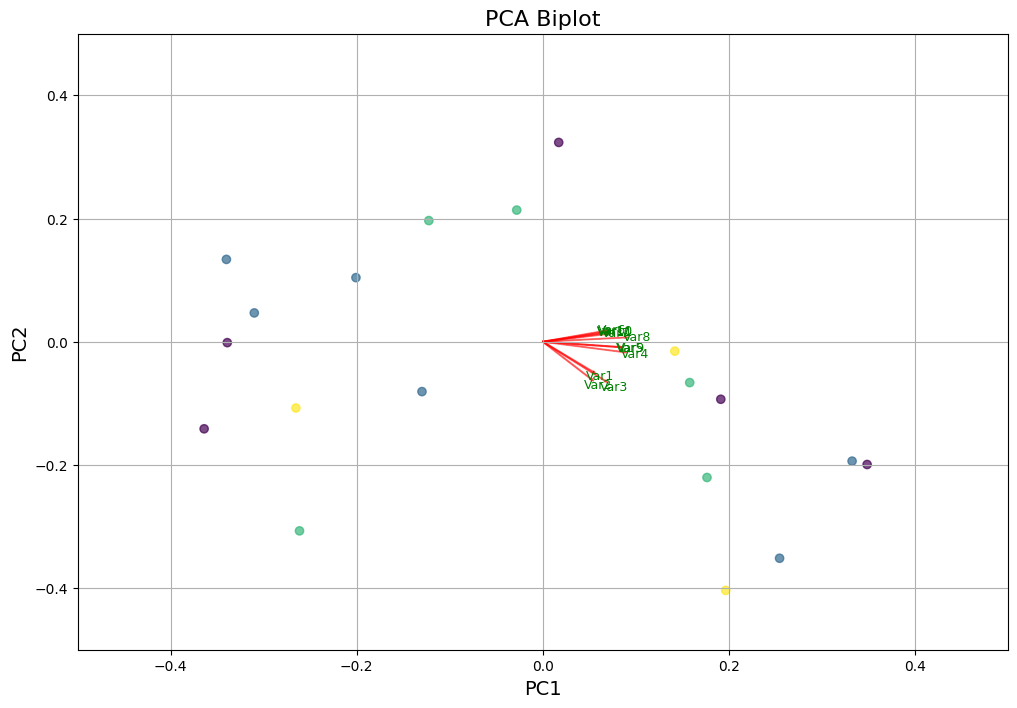
\includegraphics{03_TS_processing/03_TS_merging_final_files/figure-pdf/cell-7-output-1.pdf}

\bookmarksetup{startatroot}

\chapter{Movement annotation I: Preparing training data and data for
classifier}\label{movement-annotation-i-preparing-training-data-and-data-for-classifier}

Since we have around 9000 trials in the final dataset, it is not
feasible to manually annotate the movement onset and offset for each
trial. Instead, we will use a simple logistic regression model to
predict the movement onset and offset from all the movement features we
have collected into the merge dataset (see (\textbf{ADDREF?})).

We have annotated the movement onset and offset in (\textbf{ELAN22?})
for a pilot data (dyad 0). Two annotators have independently annotated
the movement onset and offset for four tiers: - upper body - lower body
- arms - head

Parent tier `movement' summarizes overal movement across all tiers.

Now, we will use these ground truth annotations to create a training set
for the logistic regression model.

\begin{Shaded}
\begin{Highlighting}[]
\CommentTok{\# Packages}
\ImportTok{import}\NormalTok{ os}
\ImportTok{import}\NormalTok{ glob}
\ImportTok{import}\NormalTok{ pandas }\ImportTok{as}\NormalTok{ pd}
\ImportTok{import}\NormalTok{ numpy }\ImportTok{as}\NormalTok{ np}
\ImportTok{import}\NormalTok{ xml.etree.ElementTree }\ImportTok{as}\NormalTok{ ET}
\ImportTok{import}\NormalTok{ glob}


\NormalTok{curfolder }\OperatorTok{=}\NormalTok{ os.getcwd()}

\CommentTok{\# Here we store our timeseries data}
\NormalTok{processedfolder }\OperatorTok{=}\NormalTok{ os.path.join(curfolder }\OperatorTok{+} \StringTok{\textquotesingle{}}\CharTok{\textbackslash{}\textbackslash{}}\StringTok{..}\CharTok{\textbackslash{}\textbackslash{}}\StringTok{03\_TS\_processing}\CharTok{\textbackslash{}\textbackslash{}}\StringTok{TS\_merged}\CharTok{\textbackslash{}\textbackslash{}}\StringTok{\textquotesingle{}}\NormalTok{)}
\NormalTok{processedfiles }\OperatorTok{=}\NormalTok{ glob.glob(processedfolder }\OperatorTok{+} \StringTok{\textquotesingle{}}\CharTok{\textbackslash{}\textbackslash{}}\StringTok{merged*.csv\textquotesingle{}}\NormalTok{)}
\NormalTok{processedfiles }\OperatorTok{=}\NormalTok{ [x }\ControlFlowTok{for}\NormalTok{ x }\KeywordTok{in}\NormalTok{ processedfiles }\ControlFlowTok{if} \StringTok{\textquotesingle{}anno\textquotesingle{}} \KeywordTok{not} \KeywordTok{in}\NormalTok{ x]}

\CommentTok{\# Here we will store the training data}
\NormalTok{datasetfolder }\OperatorTok{=}\NormalTok{ os.path.join(curfolder }\OperatorTok{+} \StringTok{\textquotesingle{}}\CharTok{\textbackslash{}\textbackslash{}}\StringTok{TrainingData}\CharTok{\textbackslash{}\textbackslash{}}\StringTok{\textquotesingle{}}\NormalTok{)}

\CommentTok{\# Here we store the data ready to classify}
\NormalTok{chunked\_folder }\OperatorTok{=}\NormalTok{ os.path.join(curfolder }\OperatorTok{+} \StringTok{\textquotesingle{}}\CharTok{\textbackslash{}\textbackslash{}}\StringTok{TS\_forClassifying}\CharTok{\textbackslash{}\textbackslash{}}\StringTok{\textquotesingle{}}\NormalTok{)}
\end{Highlighting}
\end{Shaded}

\bookmarksetup{startatroot}

\chapter{Preparing manual
annotations}\label{preparing-manual-annotations}

Our annotators are annotating only movement, so first we need to also
fill in the missing space by nomovement values .

\begin{Shaded}
\begin{Highlighting}[]
\CommentTok{\# Function to add no{-}movement annotations to the ELAN file}
\KeywordTok{def}\NormalTok{ add\_nomovement\_annotations(xml\_file\_path, newfilepath):}
    \CommentTok{\# Load the XML file}
\NormalTok{    tree }\OperatorTok{=}\NormalTok{ ET.parse(xml\_file\_path)}
\NormalTok{    root }\OperatorTok{=}\NormalTok{ tree.getroot()}

    \CommentTok{\# Extract all time slots}
\NormalTok{    time\_slots }\OperatorTok{=}\NormalTok{ \{\}}
    \ControlFlowTok{for}\NormalTok{ time\_slot }\KeywordTok{in}\NormalTok{ root.find(}\StringTok{\textquotesingle{}TIME\_ORDER\textquotesingle{}}\NormalTok{).findall(}\StringTok{\textquotesingle{}TIME\_SLOT\textquotesingle{}}\NormalTok{):}
\NormalTok{        time\_slots[time\_slot.attrib[}\StringTok{\textquotesingle{}TIME\_SLOT\_ID\textquotesingle{}}\NormalTok{]] }\OperatorTok{=} \BuiltInTok{int}\NormalTok{(time\_slot.attrib[}\StringTok{\textquotesingle{}TIME\_VALUE\textquotesingle{}}\NormalTok{])}

    \CommentTok{\# Sort time slots by TIME\_VALUE}
\NormalTok{    sorted\_time\_slots }\OperatorTok{=} \BuiltInTok{sorted}\NormalTok{(time\_slots.items(), key}\OperatorTok{=}\KeywordTok{lambda}\NormalTok{ x: x[}\DecValTok{1}\NormalTok{])}
\NormalTok{    time\_slot\_ids }\OperatorTok{=}\NormalTok{ [ts[}\DecValTok{0}\NormalTok{] }\ControlFlowTok{for}\NormalTok{ ts }\KeywordTok{in}\NormalTok{ sorted\_time\_slots]}
\NormalTok{    time\_values }\OperatorTok{=}\NormalTok{ [ts[}\DecValTok{1}\NormalTok{] }\ControlFlowTok{for}\NormalTok{ ts }\KeywordTok{in}\NormalTok{ sorted\_time\_slots]}

    \CommentTok{\# Loop over all tiers}
    \ControlFlowTok{for}\NormalTok{ tier }\KeywordTok{in}\NormalTok{ root.findall(}\StringTok{\textquotesingle{}TIER\textquotesingle{}}\NormalTok{):}
\NormalTok{        annotations }\OperatorTok{=}\NormalTok{ tier.findall(}\StringTok{\textquotesingle{}ANNOTATION/ALIGNABLE\_ANNOTATION\textquotesingle{}}\NormalTok{)}

        \ControlFlowTok{if} \KeywordTok{not}\NormalTok{ annotations:}
            \CommentTok{\# If no annotations exist, add a single \textquotesingle{}nomovement\textquotesingle{} annotation covering the whole tier}
\NormalTok{            new\_annotation }\OperatorTok{=}\NormalTok{ ET.Element(}\StringTok{\textquotesingle{}ANNOTATION\textquotesingle{}}\NormalTok{)}
\NormalTok{            alignable\_annotation }\OperatorTok{=}\NormalTok{ ET.SubElement(new\_annotation, }\StringTok{\textquotesingle{}ALIGNABLE\_ANNOTATION\textquotesingle{}}\NormalTok{)}
\NormalTok{            alignable\_annotation.}\BuiltInTok{set}\NormalTok{(}\StringTok{\textquotesingle{}TIME\_SLOT\_REF1\textquotesingle{}}\NormalTok{, time\_slot\_ids[}\DecValTok{0}\NormalTok{])}
\NormalTok{            alignable\_annotation.}\BuiltInTok{set}\NormalTok{(}\StringTok{\textquotesingle{}TIME\_SLOT\_REF2\textquotesingle{}}\NormalTok{, time\_slot\_ids[}\OperatorTok{{-}}\DecValTok{1}\NormalTok{])}
\NormalTok{            annotation\_value }\OperatorTok{=}\NormalTok{ ET.SubElement(alignable\_annotation, }\StringTok{\textquotesingle{}ANNOTATION\_VALUE\textquotesingle{}}\NormalTok{)}
\NormalTok{            annotation\_value.text }\OperatorTok{=} \StringTok{\textquotesingle{}nomovement\textquotesingle{}}
\NormalTok{            tier.append(new\_annotation)}
        \ControlFlowTok{else}\NormalTok{:}
            \CommentTok{\# Sort annotations by start time}
\NormalTok{            sorted\_annotations }\OperatorTok{=} \BuiltInTok{sorted}\NormalTok{(annotations, key}\OperatorTok{=}\KeywordTok{lambda}\NormalTok{ x: time\_slots[x.attrib[}\StringTok{\textquotesingle{}TIME\_SLOT\_REF1\textquotesingle{}}\NormalTok{]])}
            
            \CommentTok{\# Handle the first annotation}
\NormalTok{            first\_annotation }\OperatorTok{=}\NormalTok{ sorted\_annotations[}\DecValTok{0}\NormalTok{]}
\NormalTok{            first\_start\_time }\OperatorTok{=}\NormalTok{ time\_slots[first\_annotation.attrib[}\StringTok{\textquotesingle{}TIME\_SLOT\_REF1\textquotesingle{}}\NormalTok{]]}
            \ControlFlowTok{if}\NormalTok{ first\_start\_time }\OperatorTok{\textgreater{}}\NormalTok{ time\_values[}\DecValTok{0}\NormalTok{]:}
\NormalTok{                new\_annotation }\OperatorTok{=}\NormalTok{ ET.Element(}\StringTok{\textquotesingle{}ANNOTATION\textquotesingle{}}\NormalTok{)}
\NormalTok{                alignable\_annotation }\OperatorTok{=}\NormalTok{ ET.SubElement(new\_annotation, }\StringTok{\textquotesingle{}ALIGNABLE\_ANNOTATION\textquotesingle{}}\NormalTok{)}
\NormalTok{                alignable\_annotation.}\BuiltInTok{set}\NormalTok{(}\StringTok{\textquotesingle{}TIME\_SLOT\_REF1\textquotesingle{}}\NormalTok{, time\_slot\_ids[}\DecValTok{0}\NormalTok{])}
\NormalTok{                alignable\_annotation.}\BuiltInTok{set}\NormalTok{(}\StringTok{\textquotesingle{}TIME\_SLOT\_REF2\textquotesingle{}}\NormalTok{, first\_annotation.attrib[}\StringTok{\textquotesingle{}TIME\_SLOT\_REF1\textquotesingle{}}\NormalTok{])}
\NormalTok{                annotation\_value }\OperatorTok{=}\NormalTok{ ET.SubElement(alignable\_annotation, }\StringTok{\textquotesingle{}ANNOTATION\_VALUE\textquotesingle{}}\NormalTok{)}
\NormalTok{                annotation\_value.text }\OperatorTok{=} \StringTok{\textquotesingle{}nomovement\textquotesingle{}}
\NormalTok{                tier.append(new\_annotation)}

            \CommentTok{\# Handle gaps between annotations}
            \ControlFlowTok{for}\NormalTok{ i }\KeywordTok{in} \BuiltInTok{range}\NormalTok{(}\BuiltInTok{len}\NormalTok{(sorted\_annotations) }\OperatorTok{{-}} \DecValTok{1}\NormalTok{):}
\NormalTok{                current\_annotation }\OperatorTok{=}\NormalTok{ sorted\_annotations[i]}
\NormalTok{                next\_annotation }\OperatorTok{=}\NormalTok{ sorted\_annotations[i }\OperatorTok{+} \DecValTok{1}\NormalTok{]}
\NormalTok{                current\_end\_time }\OperatorTok{=}\NormalTok{ time\_slots[current\_annotation.attrib[}\StringTok{\textquotesingle{}TIME\_SLOT\_REF2\textquotesingle{}}\NormalTok{]]}
\NormalTok{                next\_start\_time }\OperatorTok{=}\NormalTok{ time\_slots[next\_annotation.attrib[}\StringTok{\textquotesingle{}TIME\_SLOT\_REF1\textquotesingle{}}\NormalTok{]]}
                \ControlFlowTok{if}\NormalTok{ current\_end\_time }\OperatorTok{\textless{}}\NormalTok{ next\_start\_time:}
\NormalTok{                    new\_annotation }\OperatorTok{=}\NormalTok{ ET.Element(}\StringTok{\textquotesingle{}ANNOTATION\textquotesingle{}}\NormalTok{)}
\NormalTok{                    alignable\_annotation }\OperatorTok{=}\NormalTok{ ET.SubElement(new\_annotation, }\StringTok{\textquotesingle{}ALIGNABLE\_ANNOTATION\textquotesingle{}}\NormalTok{)}
\NormalTok{                    alignable\_annotation.}\BuiltInTok{set}\NormalTok{(}\StringTok{\textquotesingle{}TIME\_SLOT\_REF1\textquotesingle{}}\NormalTok{, current\_annotation.attrib[}\StringTok{\textquotesingle{}TIME\_SLOT\_REF2\textquotesingle{}}\NormalTok{])}
\NormalTok{                    alignable\_annotation.}\BuiltInTok{set}\NormalTok{(}\StringTok{\textquotesingle{}TIME\_SLOT\_REF2\textquotesingle{}}\NormalTok{, next\_annotation.attrib[}\StringTok{\textquotesingle{}TIME\_SLOT\_REF1\textquotesingle{}}\NormalTok{])}
\NormalTok{                    annotation\_value }\OperatorTok{=}\NormalTok{ ET.SubElement(alignable\_annotation, }\StringTok{\textquotesingle{}ANNOTATION\_VALUE\textquotesingle{}}\NormalTok{)}
\NormalTok{                    annotation\_value.text }\OperatorTok{=} \StringTok{\textquotesingle{}nomovement\textquotesingle{}}
\NormalTok{                    tier.append(new\_annotation)}

            \CommentTok{\# Handle the last annotation}
\NormalTok{            last\_annotation }\OperatorTok{=}\NormalTok{ sorted\_annotations[}\OperatorTok{{-}}\DecValTok{1}\NormalTok{]}
\NormalTok{            last\_end\_time }\OperatorTok{=}\NormalTok{ time\_slots[last\_annotation.attrib[}\StringTok{\textquotesingle{}TIME\_SLOT\_REF2\textquotesingle{}}\NormalTok{]]}
            \ControlFlowTok{if}\NormalTok{ last\_end\_time }\OperatorTok{\textless{}}\NormalTok{ time\_values[}\OperatorTok{{-}}\DecValTok{1}\NormalTok{]:}
\NormalTok{                new\_annotation }\OperatorTok{=}\NormalTok{ ET.Element(}\StringTok{\textquotesingle{}ANNOTATION\textquotesingle{}}\NormalTok{)}
\NormalTok{                alignable\_annotation }\OperatorTok{=}\NormalTok{ ET.SubElement(new\_annotation, }\StringTok{\textquotesingle{}ALIGNABLE\_ANNOTATION\textquotesingle{}}\NormalTok{)}
\NormalTok{                alignable\_annotation.}\BuiltInTok{set}\NormalTok{(}\StringTok{\textquotesingle{}TIME\_SLOT\_REF1\textquotesingle{}}\NormalTok{, last\_annotation.attrib[}\StringTok{\textquotesingle{}TIME\_SLOT\_REF2\textquotesingle{}}\NormalTok{])}
\NormalTok{                alignable\_annotation.}\BuiltInTok{set}\NormalTok{(}\StringTok{\textquotesingle{}TIME\_SLOT\_REF2\textquotesingle{}}\NormalTok{, time\_slot\_ids[}\OperatorTok{{-}}\DecValTok{1}\NormalTok{])}
\NormalTok{                annotation\_value }\OperatorTok{=}\NormalTok{ ET.SubElement(alignable\_annotation, }\StringTok{\textquotesingle{}ANNOTATION\_VALUE\textquotesingle{}}\NormalTok{)}
\NormalTok{                annotation\_value.text }\OperatorTok{=} \StringTok{\textquotesingle{}nomovement\textquotesingle{}}
\NormalTok{                tier.append(new\_annotation)}

    \CommentTok{\# Save the modified XML file as a new file}
\NormalTok{    tree.write(newfilepath, encoding}\OperatorTok{=}\StringTok{\textquotesingle{}UTF{-}8\textquotesingle{}}\NormalTok{, xml\_declaration}\OperatorTok{=}\VariableTok{True}\NormalTok{)}
\end{Highlighting}
\end{Shaded}

\begin{Shaded}
\begin{Highlighting}[]
\NormalTok{manualanno\_folder\_r1 }\OperatorTok{=}\NormalTok{ curfolder }\OperatorTok{+} \StringTok{\textquotesingle{}/ManualAnno/R1/\textquotesingle{}}            \CommentTok{\# Annotator 1 (AC)}
\NormalTok{manualanno\_folder\_r3 }\OperatorTok{=}\NormalTok{ curfolder }\OperatorTok{+} \StringTok{\textquotesingle{}/ManualAnno/R3/\textquotesingle{}}            \CommentTok{\# Annotator 2 (GR)}

\NormalTok{manualannofiles1 }\OperatorTok{=}\NormalTok{ glob.glob(manualanno\_folder\_r1 }\OperatorTok{+} \StringTok{\textquotesingle{}/*.eaf\textquotesingle{}}\NormalTok{)}
\CommentTok{\# get rid of those with ELAN\_tiers.eaf}
\NormalTok{manualannofiles1 }\OperatorTok{=}\NormalTok{ [x }\ControlFlowTok{for}\NormalTok{ x }\KeywordTok{in}\NormalTok{ manualannofiles1 }\ControlFlowTok{if} \StringTok{\textquotesingle{}ELAN\_tiers\textquotesingle{}} \KeywordTok{not} \KeywordTok{in}\NormalTok{ x]}
\NormalTok{manualannofiles3 }\OperatorTok{=}\NormalTok{ glob.glob(manualanno\_folder\_r3 }\OperatorTok{+} \StringTok{\textquotesingle{}/*.eaf\textquotesingle{}}\NormalTok{)}
\CommentTok{\# get rid of those with ELAN\_tiers.eaf}
\NormalTok{manualannofiles3 }\OperatorTok{=}\NormalTok{ [x }\ControlFlowTok{for}\NormalTok{ x }\KeywordTok{in}\NormalTok{ manualannofiles3 }\ControlFlowTok{if} \StringTok{\textquotesingle{}ELAN\_tiers\textquotesingle{}} \KeywordTok{not} \KeywordTok{in}\NormalTok{ x]}


\ControlFlowTok{for} \BuiltInTok{file} \KeywordTok{in}\NormalTok{ manualannofiles3:}
    \BuiltInTok{print}\NormalTok{(}\StringTok{\textquotesingle{}working on \textquotesingle{}} \OperatorTok{+} \BuiltInTok{file}\NormalTok{)}

    \CommentTok{\# New filename is without third part of the name}
\NormalTok{    newfile }\OperatorTok{=} \BuiltInTok{file}\NormalTok{.split(}\StringTok{\textquotesingle{}}\CharTok{\textbackslash{}\textbackslash{}}\StringTok{\textquotesingle{}}\NormalTok{)[}\OperatorTok{{-}}\DecValTok{1}\NormalTok{]}
\NormalTok{    chunks }\OperatorTok{=}\NormalTok{ newfile.split(}\StringTok{\textquotesingle{}\_\textquotesingle{}}\NormalTok{)}
    \ControlFlowTok{if} \StringTok{\textquotesingle{}corrected\textquotesingle{}} \KeywordTok{in} \BuiltInTok{file}\NormalTok{:}
        \ControlFlowTok{if} \StringTok{\textquotesingle{}c0\textquotesingle{}} \KeywordTok{in} \BuiltInTok{file} \KeywordTok{or} \StringTok{\textquotesingle{}c1\textquotesingle{}} \KeywordTok{in} \BuiltInTok{file} \KeywordTok{or} \StringTok{\textquotesingle{}c2\textquotesingle{}} \KeywordTok{in} \BuiltInTok{file}\NormalTok{:}
\NormalTok{            newfile }\OperatorTok{=} \StringTok{\textquotesingle{}\_\textquotesingle{}}\NormalTok{.join(chunks[:}\OperatorTok{{-}}\DecValTok{4}\NormalTok{])}
        \ControlFlowTok{else}\NormalTok{:}
\NormalTok{            newfile }\OperatorTok{=} \StringTok{\textquotesingle{}\_\textquotesingle{}}\NormalTok{.join(chunks[:}\OperatorTok{{-}}\DecValTok{3}\NormalTok{])}
    \ControlFlowTok{else}\NormalTok{:}
        \ControlFlowTok{if} \StringTok{\textquotesingle{}c0\textquotesingle{}} \KeywordTok{in} \BuiltInTok{file} \KeywordTok{or} \StringTok{\textquotesingle{}c1\textquotesingle{}} \KeywordTok{in} \BuiltInTok{file} \KeywordTok{or} \StringTok{\textquotesingle{}c2\textquotesingle{}} \KeywordTok{in} \BuiltInTok{file}\NormalTok{:}
\NormalTok{            newfile }\OperatorTok{=} \StringTok{\textquotesingle{}\_\textquotesingle{}}\NormalTok{.join(chunks[:}\OperatorTok{{-}}\DecValTok{3}\NormalTok{])}
        \ControlFlowTok{else}\NormalTok{:}
\NormalTok{            newfile }\OperatorTok{=} \StringTok{\textquotesingle{}\_\textquotesingle{}}\NormalTok{.join(chunks[:}\OperatorTok{{-}}\DecValTok{2}\NormalTok{]) }

\NormalTok{    newfile }\OperatorTok{=}\NormalTok{ newfile.replace(}\StringTok{\textquotesingle{}trial\_\textquotesingle{}}\NormalTok{, }\StringTok{\textquotesingle{}\textquotesingle{}}\NormalTok{)}
    
    \CommentTok{\# Save it again}
\NormalTok{    newfile }\OperatorTok{=}\NormalTok{ manualanno\_folder\_r3 }\OperatorTok{+}\NormalTok{ newfile }\OperatorTok{+} \StringTok{\textquotesingle{}\_ELAN\_tiers.eaf\textquotesingle{}}

\NormalTok{    add\_nomovement\_annotations(}\BuiltInTok{file}\NormalTok{, newfile)}
\end{Highlighting}
\end{Shaded}

Now, we need to get the manual annotation from ELAN to simple text file
so that we can merge the timeseries we prepared in (\textbf{ADDREF?})
with information about movement in the trial

\begin{Shaded}
\begin{Highlighting}[]
\CommentTok{\# Function to parse elan file}
\KeywordTok{def}\NormalTok{ parse\_eaf\_file(eaf\_file, rel\_tiers):}
\NormalTok{    tree }\OperatorTok{=}\NormalTok{ ET.parse(eaf\_file)}
\NormalTok{    root }\OperatorTok{=}\NormalTok{ tree.getroot()}

\NormalTok{    time\_order }\OperatorTok{=}\NormalTok{ root.find(}\StringTok{\textquotesingle{}TIME\_ORDER\textquotesingle{}}\NormalTok{)}
\NormalTok{    time\_slots }\OperatorTok{=}\NormalTok{ \{time\_slot.attrib[}\StringTok{\textquotesingle{}TIME\_SLOT\_ID\textquotesingle{}}\NormalTok{]: time\_slot.attrib[}\StringTok{\textquotesingle{}TIME\_VALUE\textquotesingle{}}\NormalTok{] }\ControlFlowTok{for}\NormalTok{ time\_slot }\KeywordTok{in}\NormalTok{ time\_order\}}

\NormalTok{    annotations }\OperatorTok{=}\NormalTok{ []}
\NormalTok{    relevant\_tiers }\OperatorTok{=}\NormalTok{ \{rel\_tiers\}}

    \ControlFlowTok{for}\NormalTok{ tier }\KeywordTok{in}\NormalTok{ root.findall(}\StringTok{\textquotesingle{}TIER\textquotesingle{}}\NormalTok{):}
\NormalTok{        tier\_id }\OperatorTok{=}\NormalTok{ tier.attrib[}\StringTok{\textquotesingle{}TIER\_ID\textquotesingle{}}\NormalTok{]}
        \ControlFlowTok{if}\NormalTok{ tier\_id }\KeywordTok{in}\NormalTok{ relevant\_tiers:}
            \ControlFlowTok{for}\NormalTok{ annotation }\KeywordTok{in}\NormalTok{ tier.findall(}\StringTok{\textquotesingle{}ANNOTATION/ALIGNABLE\_ANNOTATION\textquotesingle{}}\NormalTok{):}
                \CommentTok{\# Ensure required attributes are present}
                \ControlFlowTok{if} \StringTok{\textquotesingle{}TIME\_SLOT\_REF1\textquotesingle{}} \KeywordTok{in}\NormalTok{ annotation.attrib }\KeywordTok{and} \StringTok{\textquotesingle{}TIME\_SLOT\_REF2\textquotesingle{}} \KeywordTok{in}\NormalTok{ annotation.attrib:}
\NormalTok{                    ts\_ref1 }\OperatorTok{=}\NormalTok{ annotation.attrib[}\StringTok{\textquotesingle{}TIME\_SLOT\_REF1\textquotesingle{}}\NormalTok{]}
\NormalTok{                    ts\_ref2 }\OperatorTok{=}\NormalTok{ annotation.attrib[}\StringTok{\textquotesingle{}TIME\_SLOT\_REF2\textquotesingle{}}\NormalTok{]}
                    \CommentTok{\# Get annotation ID if it exists, otherwise set to None}
\NormalTok{                    ann\_id }\OperatorTok{=}\NormalTok{ annotation.attrib.get(}\StringTok{\textquotesingle{}ANNOTATION\_ID\textquotesingle{}}\NormalTok{, }\VariableTok{None}\NormalTok{)}
\NormalTok{                    annotation\_value }\OperatorTok{=}\NormalTok{ annotation.find(}\StringTok{\textquotesingle{}ANNOTATION\_VALUE\textquotesingle{}}\NormalTok{).text.strip()}
\NormalTok{                    annotations.append(\{}
                        \StringTok{\textquotesingle{}tier\_id\textquotesingle{}}\NormalTok{: tier\_id,}
                        \StringTok{\textquotesingle{}annotation\_id\textquotesingle{}}\NormalTok{: ann\_id,}
                        \StringTok{\textquotesingle{}start\_time\textquotesingle{}}\NormalTok{: time\_slots[ts\_ref1],}
                        \StringTok{\textquotesingle{}end\_time\textquotesingle{}}\NormalTok{: time\_slots[ts\_ref2],}
                        \StringTok{\textquotesingle{}annotation\_value\textquotesingle{}}\NormalTok{: annotation\_value}
\NormalTok{                    \})}

    \ControlFlowTok{return}\NormalTok{ annotations}

\CommentTok{\# Function to load annotations into csv}
\KeywordTok{def}\NormalTok{ fillAnno(TSfile, ANNOfile, colname):}
\NormalTok{    TSfile[colname] }\OperatorTok{=} \VariableTok{None}
    \ControlFlowTok{for}\NormalTok{ row }\KeywordTok{in}\NormalTok{ ANNOfile.iterrows():}
\NormalTok{        start }\OperatorTok{=}\NormalTok{ row[}\DecValTok{1}\NormalTok{][}\DecValTok{0}\NormalTok{]}
\NormalTok{        end }\OperatorTok{=}\NormalTok{ row[}\DecValTok{1}\NormalTok{][}\DecValTok{1}\NormalTok{]}
\NormalTok{        TSfile.loc[(TSfile[}\StringTok{\textquotesingle{}time\textquotesingle{}}\NormalTok{] }\OperatorTok{\textgreater{}=}\NormalTok{ start) }\OperatorTok{\&}\NormalTok{ (TSfile[}\StringTok{\textquotesingle{}time\textquotesingle{}}\NormalTok{] }\OperatorTok{\textless{}=}\NormalTok{ end), colname] }\OperatorTok{=}\NormalTok{ row[}\DecValTok{1}\NormalTok{][}\DecValTok{2}\NormalTok{]}
\end{Highlighting}
\end{Shaded}

Now we create text file for each tier separately, saving only the start
time, end time and value (movement or nomovement) for each annotation
file.

\begin{Shaded}
\begin{Highlighting}[]
\CommentTok{\# These are the manual annotations adapted with no{-}movement annotations}
\NormalTok{annofolder\_manu }\OperatorTok{=}\NormalTok{ os.path.join(curfolder }\OperatorTok{+} \StringTok{\textquotesingle{}}\CharTok{\textbackslash{}\textbackslash{}}\StringTok{ManualAnno}\CharTok{\textbackslash{}\textbackslash{}}\StringTok{R1}\CharTok{\textbackslash{}\textbackslash{}}\StringTok{\textquotesingle{}}\NormalTok{)}
\NormalTok{annofiles\_manu }\OperatorTok{=}\NormalTok{ glob.glob(annofolder\_manu }\OperatorTok{+} \StringTok{\textquotesingle{}*ELAN\_tiers.eaf\textquotesingle{}}\NormalTok{)}

\CommentTok{\#\#\#\#\#\#\#\#\#\#\#\#\#\#\#\#}
\CommentTok{\#\#\#\# arms \#\#\#\#\#\#}
\CommentTok{\#\#\#\#\#\#\#\#\#\#\#\#\#\#\#\#}

\NormalTok{arms\_anno }\OperatorTok{=}\NormalTok{ curfolder }\OperatorTok{+} \StringTok{\textquotesingle{}/annotations\_groundTruth/arms\_annotations.txt\textquotesingle{}}

\ControlFlowTok{with} \BuiltInTok{open}\NormalTok{(arms\_anno, }\StringTok{\textquotesingle{}w\textquotesingle{}}\NormalTok{) }\ImportTok{as}\NormalTok{ f:}
    \ControlFlowTok{for} \BuiltInTok{file} \KeywordTok{in}\NormalTok{ annofiles\_manu:}
        \BuiltInTok{print}\NormalTok{(}\StringTok{\textquotesingle{}working on \textquotesingle{}} \OperatorTok{+} \BuiltInTok{file}\NormalTok{)}
        \CommentTok{\# get the filename as the last element}
\NormalTok{        filename }\OperatorTok{=} \BuiltInTok{file}\NormalTok{.split(}\StringTok{\textquotesingle{}}\CharTok{\textbackslash{}\textbackslash{}}\StringTok{\textquotesingle{}}\NormalTok{)[}\OperatorTok{{-}}\DecValTok{1}\NormalTok{]}
        \CommentTok{\# replace \_ELAN\_tiers.eaf with \textquotesingle{}\textquotesingle{}}
\NormalTok{        filename }\OperatorTok{=}\NormalTok{ filename.replace(}\StringTok{\textquotesingle{}\_ELAN\_tiers.eaf\textquotesingle{}}\NormalTok{, }\StringTok{\textquotesingle{}\textquotesingle{}}\NormalTok{)}
        \CommentTok{\# parse the file}
\NormalTok{        annotations }\OperatorTok{=}\NormalTok{ parse\_eaf\_file(}\BuiltInTok{file}\NormalTok{, }\StringTok{\textquotesingle{}arms\textquotesingle{}}\NormalTok{)}
        \CommentTok{\# write the annotations}
        \ControlFlowTok{for}\NormalTok{ annotation }\KeywordTok{in}\NormalTok{ annotations:}
\NormalTok{            f.write(}\SpecialStringTok{f"}\SpecialCharTok{\{}\NormalTok{annotation[}\StringTok{\textquotesingle{}start\_time\textquotesingle{}}\NormalTok{]}\SpecialCharTok{\}}\CharTok{\textbackslash{}t}\SpecialCharTok{\{}\NormalTok{annotation[}\StringTok{\textquotesingle{}end\_time\textquotesingle{}}\NormalTok{]}\SpecialCharTok{\}}\CharTok{\textbackslash{}t}\SpecialCharTok{\{}\NormalTok{annotation[}\StringTok{\textquotesingle{}annotation\_value\textquotesingle{}}\NormalTok{]}\SpecialCharTok{\}}\CharTok{\textbackslash{}t}\SpecialCharTok{\{}\NormalTok{filename}\SpecialCharTok{\}}\CharTok{\textbackslash{}n}\SpecialStringTok{"}\NormalTok{)}

\CommentTok{\#\#\#\#\#\#\#\#\#\#\#\#\#\#\#\#\#\#\#}
\CommentTok{\#\#\#\# upper body\#\#\#\#}
\CommentTok{\#\#\#\#\#\#\#\#\#\#\#\#\#\#\#\#\#\#\#}

\NormalTok{upperbody\_anno }\OperatorTok{=}\NormalTok{ curfolder }\OperatorTok{+} \StringTok{\textquotesingle{}/annotations\_groundTruth/upperbody\_annotations.txt\textquotesingle{}}

\ControlFlowTok{with} \BuiltInTok{open}\NormalTok{(upperbody\_anno, }\StringTok{\textquotesingle{}w\textquotesingle{}}\NormalTok{) }\ImportTok{as}\NormalTok{ f:}
    \ControlFlowTok{for} \BuiltInTok{file} \KeywordTok{in}\NormalTok{ annofiles\_manu:}
        \BuiltInTok{print}\NormalTok{(}\StringTok{\textquotesingle{}working on \textquotesingle{}} \OperatorTok{+} \BuiltInTok{file}\NormalTok{)}
        \CommentTok{\# get the filename as the last element}
\NormalTok{        filename }\OperatorTok{=} \BuiltInTok{file}\NormalTok{.split(}\StringTok{\textquotesingle{}}\CharTok{\textbackslash{}\textbackslash{}}\StringTok{\textquotesingle{}}\NormalTok{)[}\OperatorTok{{-}}\DecValTok{1}\NormalTok{]}
        \CommentTok{\# replace \_ELAN\_tiers.eaf with \textquotesingle{}\textquotesingle{}}
\NormalTok{        filename }\OperatorTok{=}\NormalTok{ filename.replace(}\StringTok{\textquotesingle{}\_ELAN\_tiers.eaf\textquotesingle{}}\NormalTok{, }\StringTok{\textquotesingle{}\textquotesingle{}}\NormalTok{)}
        \CommentTok{\# parse the file}
\NormalTok{        annotations }\OperatorTok{=}\NormalTok{ parse\_eaf\_file(}\BuiltInTok{file}\NormalTok{, }\StringTok{\textquotesingle{}upper\_body\textquotesingle{}}\NormalTok{)}
        \CommentTok{\# write the annotations}
        \ControlFlowTok{for}\NormalTok{ annotation }\KeywordTok{in}\NormalTok{ annotations:}
\NormalTok{            f.write(}\SpecialStringTok{f"}\SpecialCharTok{\{}\NormalTok{annotation[}\StringTok{\textquotesingle{}start\_time\textquotesingle{}}\NormalTok{]}\SpecialCharTok{\}}\CharTok{\textbackslash{}t}\SpecialCharTok{\{}\NormalTok{annotation[}\StringTok{\textquotesingle{}end\_time\textquotesingle{}}\NormalTok{]}\SpecialCharTok{\}}\CharTok{\textbackslash{}t}\SpecialCharTok{\{}\NormalTok{annotation[}\StringTok{\textquotesingle{}annotation\_value\textquotesingle{}}\NormalTok{]}\SpecialCharTok{\}}\CharTok{\textbackslash{}t}\SpecialCharTok{\{}\NormalTok{filename}\SpecialCharTok{\}}\CharTok{\textbackslash{}n}\SpecialStringTok{"}\NormalTok{)}

\CommentTok{\#\#\#\#\#\#\#\#\#\#\#\#\#\#\#\#\#\#\#}
\CommentTok{\#\#\#\# lower body\#\#\#\#}
\CommentTok{\#\#\#\#\#\#\#\#\#\#\#\#\#\#\#\#\#\#\#}

\NormalTok{lowerbody\_anno }\OperatorTok{=}\NormalTok{ curfolder }\OperatorTok{+} \StringTok{\textquotesingle{}/annotations\_groundTruth/lowerbody\_annotations.txt\textquotesingle{}}

\ControlFlowTok{with} \BuiltInTok{open}\NormalTok{(lowerbody\_anno, }\StringTok{\textquotesingle{}w\textquotesingle{}}\NormalTok{) }\ImportTok{as}\NormalTok{ f:}
    \ControlFlowTok{for} \BuiltInTok{file} \KeywordTok{in}\NormalTok{ annofiles\_manu:}
        \BuiltInTok{print}\NormalTok{(}\StringTok{\textquotesingle{}working on \textquotesingle{}} \OperatorTok{+} \BuiltInTok{file}\NormalTok{)}
        \CommentTok{\# get the filename as the last element}
\NormalTok{        filename }\OperatorTok{=} \BuiltInTok{file}\NormalTok{.split(}\StringTok{\textquotesingle{}}\CharTok{\textbackslash{}\textbackslash{}}\StringTok{\textquotesingle{}}\NormalTok{)[}\OperatorTok{{-}}\DecValTok{1}\NormalTok{]}
        \CommentTok{\# replace \_ELAN\_tiers.eaf with \textquotesingle{}\textquotesingle{}}
\NormalTok{        filename }\OperatorTok{=}\NormalTok{ filename.replace(}\StringTok{\textquotesingle{}\_ELAN\_tiers.eaf\textquotesingle{}}\NormalTok{, }\StringTok{\textquotesingle{}\textquotesingle{}}\NormalTok{)}
        \CommentTok{\# parse the file}
\NormalTok{        annotations }\OperatorTok{=}\NormalTok{ parse\_eaf\_file(}\BuiltInTok{file}\NormalTok{, }\StringTok{\textquotesingle{}lower\_body\textquotesingle{}}\NormalTok{)}
        \CommentTok{\# write the annotations}
        \ControlFlowTok{for}\NormalTok{ annotation }\KeywordTok{in}\NormalTok{ annotations:}
\NormalTok{            f.write(}\SpecialStringTok{f"}\SpecialCharTok{\{}\NormalTok{annotation[}\StringTok{\textquotesingle{}start\_time\textquotesingle{}}\NormalTok{]}\SpecialCharTok{\}}\CharTok{\textbackslash{}t}\SpecialCharTok{\{}\NormalTok{annotation[}\StringTok{\textquotesingle{}end\_time\textquotesingle{}}\NormalTok{]}\SpecialCharTok{\}}\CharTok{\textbackslash{}t}\SpecialCharTok{\{}\NormalTok{annotation[}\StringTok{\textquotesingle{}annotation\_value\textquotesingle{}}\NormalTok{]}\SpecialCharTok{\}}\CharTok{\textbackslash{}t}\SpecialCharTok{\{}\NormalTok{filename}\SpecialCharTok{\}}\CharTok{\textbackslash{}n}\SpecialStringTok{"}\NormalTok{)}

\CommentTok{\#\#\#\#\#\#\#\#\#\#\#\#\#\#\#\#\#\#\#}
\CommentTok{\#\#\#\#\# head \#\#\#\#\#\#\#\#}
\CommentTok{\#\#\#\#\#\#\#\#\#\#\#\#\#\#\#\#\#\#\#}

\NormalTok{head\_anno }\OperatorTok{=}\NormalTok{ curfolder }\OperatorTok{+} \StringTok{\textquotesingle{}/annotations\_groundTruth/head\_annotations.txt\textquotesingle{}}

\ControlFlowTok{with} \BuiltInTok{open}\NormalTok{(head\_anno, }\StringTok{\textquotesingle{}w\textquotesingle{}}\NormalTok{) }\ImportTok{as}\NormalTok{ f:}
    \ControlFlowTok{for} \BuiltInTok{file} \KeywordTok{in}\NormalTok{ annofiles\_manu:}
        \BuiltInTok{print}\NormalTok{(}\StringTok{\textquotesingle{}working on \textquotesingle{}} \OperatorTok{+} \BuiltInTok{file}\NormalTok{)}
        \CommentTok{\# get the filename as the last element}
\NormalTok{        filename }\OperatorTok{=} \BuiltInTok{file}\NormalTok{.split(}\StringTok{\textquotesingle{}}\CharTok{\textbackslash{}\textbackslash{}}\StringTok{\textquotesingle{}}\NormalTok{)[}\OperatorTok{{-}}\DecValTok{1}\NormalTok{]}
        \CommentTok{\# replace \_ELAN\_tiers.eaf with \textquotesingle{}\textquotesingle{}}
\NormalTok{        filename }\OperatorTok{=}\NormalTok{ filename.replace(}\StringTok{\textquotesingle{}\_ELAN\_tiers.eaf\textquotesingle{}}\NormalTok{, }\StringTok{\textquotesingle{}\textquotesingle{}}\NormalTok{)}
        \CommentTok{\# parse the file}
\NormalTok{        annotations }\OperatorTok{=}\NormalTok{ parse\_eaf\_file(}\BuiltInTok{file}\NormalTok{, }\StringTok{\textquotesingle{}head\_mov\textquotesingle{}}\NormalTok{)}
        \CommentTok{\# write the annotations}
        \ControlFlowTok{for}\NormalTok{ annotation }\KeywordTok{in}\NormalTok{ annotations:}
\NormalTok{            f.write(}\SpecialStringTok{f"}\SpecialCharTok{\{}\NormalTok{annotation[}\StringTok{\textquotesingle{}start\_time\textquotesingle{}}\NormalTok{]}\SpecialCharTok{\}}\CharTok{\textbackslash{}t}\SpecialCharTok{\{}\NormalTok{annotation[}\StringTok{\textquotesingle{}end\_time\textquotesingle{}}\NormalTok{]}\SpecialCharTok{\}}\CharTok{\textbackslash{}t}\SpecialCharTok{\{}\NormalTok{annotation[}\StringTok{\textquotesingle{}annotation\_value\textquotesingle{}}\NormalTok{]}\SpecialCharTok{\}}\CharTok{\textbackslash{}t}\SpecialCharTok{\{}\NormalTok{filename}\SpecialCharTok{\}}\CharTok{\textbackslash{}n}\SpecialStringTok{"}\NormalTok{)}
\end{Highlighting}
\end{Shaded}

\bookmarksetup{startatroot}

\chapter{Preparing data for
classifier}\label{preparing-data-for-classifier}

In the following code, we merge the annotations with our merged files
(created in (\textbf{ADDREF?})) so that we can later sample from the
data based on the annotations.

We will now also filter some superfluous information, as well as add
some more, such as:

\begin{itemize}
\tightlist
\item
  distance of LIndex to RIndex
\item
  distance of Wrist to Hip
\item
  distance of Head to Hip
\item
  distance of Head to Ankle
\end{itemize}

\begin{Shaded}
\begin{Highlighting}[]
\CommentTok{\# These are the annotations per tier that we just created from manual annotations}
\NormalTok{arms\_anno }\OperatorTok{=}\NormalTok{ curfolder }\OperatorTok{+} \StringTok{\textquotesingle{}/annotations\_groundTruth/arms\_annotations.txt\textquotesingle{}}
\NormalTok{upperbody\_anno }\OperatorTok{=}\NormalTok{ curfolder }\OperatorTok{+} \StringTok{\textquotesingle{}/annotations\_groundTruth/upperbody\_annotations.txt\textquotesingle{}}
\NormalTok{lowerbody\_anno }\OperatorTok{=}\NormalTok{ curfolder }\OperatorTok{+} \StringTok{\textquotesingle{}/annotations\_groundTruth/lowerbody\_annotations.txt\textquotesingle{}}
\NormalTok{head\_anno }\OperatorTok{=}\NormalTok{ curfolder }\OperatorTok{+} \StringTok{\textquotesingle{}/annotations\_groundTruth/head\_annotations.txt\textquotesingle{}}

\ControlFlowTok{for} \BuiltInTok{file} \KeywordTok{in}\NormalTok{ processedfiles:}

    \CommentTok{\# TrialID}
\NormalTok{    trialid }\OperatorTok{=} \BuiltInTok{file}\NormalTok{.split(}\StringTok{\textquotesingle{}}\CharTok{\textbackslash{}\textbackslash{}}\StringTok{\textquotesingle{}}\NormalTok{)[}\OperatorTok{{-}}\DecValTok{1}\NormalTok{].split(}\StringTok{\textquotesingle{}.\textquotesingle{}}\NormalTok{)[}\DecValTok{0}\NormalTok{]}
\NormalTok{    trialid }\OperatorTok{=}\NormalTok{ trialid.replace(}\StringTok{\textquotesingle{}merged\_\textquotesingle{}}\NormalTok{, }\StringTok{\textquotesingle{}\textquotesingle{}}\NormalTok{)}

    \BuiltInTok{print}\NormalTok{(}\StringTok{\textquotesingle{}working on \textquotesingle{}} \OperatorTok{+}\NormalTok{ trialid)}

    \CommentTok{\# Load the merged file}
\NormalTok{    merged }\OperatorTok{=}\NormalTok{ pd.read\_csv(}\BuiltInTok{file}\NormalTok{)}
    
    \CommentTok{\# Load the annotations as df}
\NormalTok{    arms }\OperatorTok{=}\NormalTok{ pd.read\_csv(arms\_anno, sep}\OperatorTok{=}\StringTok{\textquotesingle{}}\CharTok{\textbackslash{}t}\StringTok{\textquotesingle{}}\NormalTok{, header}\OperatorTok{=}\VariableTok{None}\NormalTok{)}
\NormalTok{    ub }\OperatorTok{=}\NormalTok{ pd.read\_csv(upperbody\_anno, sep}\OperatorTok{=}\StringTok{\textquotesingle{}}\CharTok{\textbackslash{}t}\StringTok{\textquotesingle{}}\NormalTok{, header}\OperatorTok{=}\VariableTok{None}\NormalTok{)}
\NormalTok{    lb }\OperatorTok{=}\NormalTok{ pd.read\_csv(lowerbody\_anno, sep}\OperatorTok{=}\StringTok{\textquotesingle{}}\CharTok{\textbackslash{}t}\StringTok{\textquotesingle{}}\NormalTok{, header}\OperatorTok{=}\VariableTok{None}\NormalTok{)}
\NormalTok{    head }\OperatorTok{=}\NormalTok{ pd.read\_csv(head\_anno, sep}\OperatorTok{=}\StringTok{\textquotesingle{}}\CharTok{\textbackslash{}t}\StringTok{\textquotesingle{}}\NormalTok{, header}\OperatorTok{=}\VariableTok{None}\NormalTok{)}

\NormalTok{    annos }\OperatorTok{=}\NormalTok{ [arms, ub, lb, head]}

\NormalTok{    practice }\OperatorTok{=} \VariableTok{False}

    \CommentTok{\# Loop over each tier and fill values into timeseries}
    \ControlFlowTok{for}\NormalTok{ anno\_df }\KeywordTok{in}\NormalTok{ annos:}
        \CommentTok{\# Get the annotations for the trialid}
\NormalTok{        anno\_trial }\OperatorTok{=}\NormalTok{ anno\_df[anno\_df[}\DecValTok{3}\NormalTok{] }\OperatorTok{==}\NormalTok{ trialid] }
        
        \ControlFlowTok{if}\NormalTok{ anno\_trial.empty:}
            \BuiltInTok{print}\NormalTok{(}\StringTok{\textquotesingle{}no annotations for \textquotesingle{}} \OperatorTok{+}\NormalTok{ trialid)  }\CommentTok{\# This will be the case of practice trials that were not annotated}
\NormalTok{            practice }\OperatorTok{=} \VariableTok{True}
            \ControlFlowTok{continue}
        
        \ControlFlowTok{else}\NormalTok{:}
            \ControlFlowTok{if}\NormalTok{ anno\_df.equals(arms):}
\NormalTok{                fillAnno(merged, anno\_trial, }\StringTok{\textquotesingle{}arms\textquotesingle{}}\NormalTok{)}
            \ControlFlowTok{elif}\NormalTok{ anno\_df.equals(ub):}
\NormalTok{                fillAnno(merged, anno\_trial, }\StringTok{\textquotesingle{}upper\_body\textquotesingle{}}\NormalTok{)}
            \ControlFlowTok{elif}\NormalTok{ anno\_df.equals(lb):}
\NormalTok{                fillAnno(merged, anno\_trial, }\StringTok{\textquotesingle{}lower\_body\textquotesingle{}}\NormalTok{)}
            \ControlFlowTok{elif}\NormalTok{ anno\_df.equals(head):}
\NormalTok{                fillAnno(merged, anno\_trial, }\StringTok{\textquotesingle{}head\_mov\textquotesingle{}}\NormalTok{)}
            \ControlFlowTok{else}\NormalTok{:}
                \BuiltInTok{print}\NormalTok{(}\StringTok{\textquotesingle{}something went wrong\textquotesingle{}}\NormalTok{)}

    \ControlFlowTok{if}\NormalTok{ practice:}
        \ControlFlowTok{continue}

\NormalTok{    df }\OperatorTok{=}\NormalTok{ merged.copy()}

    \CommentTok{\# Now we will also add some features that might be relevant for the classifier}
    \CommentTok{\#\# RWrist to LWrist in all dimensions}
\NormalTok{    df[}\StringTok{\textquotesingle{}wristDistance\_x\textquotesingle{}}\NormalTok{] }\OperatorTok{=}\NormalTok{ df[}\StringTok{\textquotesingle{}RWrist\_x\textquotesingle{}}\NormalTok{] }\OperatorTok{{-}}\NormalTok{ df[}\StringTok{\textquotesingle{}LWrist\_x\textquotesingle{}}\NormalTok{]}
\NormalTok{    df[}\StringTok{\textquotesingle{}wristDistance\_y\textquotesingle{}}\NormalTok{] }\OperatorTok{=}\NormalTok{ df[}\StringTok{\textquotesingle{}RWrist\_y\textquotesingle{}}\NormalTok{] }\OperatorTok{{-}}\NormalTok{ df[}\StringTok{\textquotesingle{}LWrist\_y\textquotesingle{}}\NormalTok{]}
\NormalTok{    df[}\StringTok{\textquotesingle{}wristDistance\_z\textquotesingle{}}\NormalTok{] }\OperatorTok{=}\NormalTok{ df[}\StringTok{\textquotesingle{}RWrist\_z\textquotesingle{}}\NormalTok{] }\OperatorTok{{-}}\NormalTok{ df[}\StringTok{\textquotesingle{}LWrist\_z\textquotesingle{}}\NormalTok{]}

    \CommentTok{\#\# RWrist to RHip}
\NormalTok{    df[}\StringTok{\textquotesingle{}RwristRhipDistance\_x\textquotesingle{}}\NormalTok{] }\OperatorTok{=}\NormalTok{ df[}\StringTok{\textquotesingle{}RWrist\_x\textquotesingle{}}\NormalTok{] }\OperatorTok{{-}}\NormalTok{ df[}\StringTok{\textquotesingle{}RHip\_x\textquotesingle{}}\NormalTok{]}
\NormalTok{    df[}\StringTok{\textquotesingle{}RwristRhipDistance\_y\textquotesingle{}}\NormalTok{] }\OperatorTok{=}\NormalTok{ df[}\StringTok{\textquotesingle{}RWrist\_y\textquotesingle{}}\NormalTok{] }\OperatorTok{{-}}\NormalTok{ df[}\StringTok{\textquotesingle{}RHip\_y\textquotesingle{}}\NormalTok{]}
\NormalTok{    df[}\StringTok{\textquotesingle{}RwristRhipDistance\_z\textquotesingle{}}\NormalTok{] }\OperatorTok{=}\NormalTok{ df[}\StringTok{\textquotesingle{}RWrist\_z\textquotesingle{}}\NormalTok{] }\OperatorTok{{-}}\NormalTok{ df[}\StringTok{\textquotesingle{}RHip\_z\textquotesingle{}}\NormalTok{]}

    \CommentTok{\#\# RWrist to LHip}
\NormalTok{    df[}\StringTok{\textquotesingle{}RwristLhipDistance\_x\textquotesingle{}}\NormalTok{] }\OperatorTok{=}\NormalTok{ df[}\StringTok{\textquotesingle{}RWrist\_x\textquotesingle{}}\NormalTok{] }\OperatorTok{{-}}\NormalTok{ df[}\StringTok{\textquotesingle{}LHip\_x\textquotesingle{}}\NormalTok{]}
\NormalTok{    df[}\StringTok{\textquotesingle{}RwristLhipDistance\_y\textquotesingle{}}\NormalTok{] }\OperatorTok{=}\NormalTok{ df[}\StringTok{\textquotesingle{}RWrist\_y\textquotesingle{}}\NormalTok{] }\OperatorTok{{-}}\NormalTok{ df[}\StringTok{\textquotesingle{}LHip\_y\textquotesingle{}}\NormalTok{]}
\NormalTok{    df[}\StringTok{\textquotesingle{}RwristLhipDistance\_z\textquotesingle{}}\NormalTok{] }\OperatorTok{=}\NormalTok{ df[}\StringTok{\textquotesingle{}RWrist\_z\textquotesingle{}}\NormalTok{] }\OperatorTok{{-}}\NormalTok{ df[}\StringTok{\textquotesingle{}LHip\_z\textquotesingle{}}\NormalTok{]}

    \CommentTok{\#\# LWrist to LHip}
\NormalTok{    df[}\StringTok{\textquotesingle{}LwristLhipDistance\_x\textquotesingle{}}\NormalTok{] }\OperatorTok{=}\NormalTok{ df[}\StringTok{\textquotesingle{}LWrist\_x\textquotesingle{}}\NormalTok{] }\OperatorTok{{-}}\NormalTok{ df[}\StringTok{\textquotesingle{}LHip\_x\textquotesingle{}}\NormalTok{]}
\NormalTok{    df[}\StringTok{\textquotesingle{}LwristLhipDistance\_y\textquotesingle{}}\NormalTok{] }\OperatorTok{=}\NormalTok{ df[}\StringTok{\textquotesingle{}LWrist\_y\textquotesingle{}}\NormalTok{] }\OperatorTok{{-}}\NormalTok{ df[}\StringTok{\textquotesingle{}LHip\_y\textquotesingle{}}\NormalTok{]}
\NormalTok{    df[}\StringTok{\textquotesingle{}LwristLhipDistance\_z\textquotesingle{}}\NormalTok{] }\OperatorTok{=}\NormalTok{ df[}\StringTok{\textquotesingle{}LWrist\_z\textquotesingle{}}\NormalTok{] }\OperatorTok{{-}}\NormalTok{ df[}\StringTok{\textquotesingle{}LHip\_z\textquotesingle{}}\NormalTok{]}

    \CommentTok{\#\# LWrist to RHip}
\NormalTok{    df[}\StringTok{\textquotesingle{}LwristRhipDistance\_x\textquotesingle{}}\NormalTok{] }\OperatorTok{=}\NormalTok{ df[}\StringTok{\textquotesingle{}LWrist\_x\textquotesingle{}}\NormalTok{] }\OperatorTok{{-}}\NormalTok{ df[}\StringTok{\textquotesingle{}RHip\_x\textquotesingle{}}\NormalTok{]}
\NormalTok{    df[}\StringTok{\textquotesingle{}LwristRhipDistance\_y\textquotesingle{}}\NormalTok{] }\OperatorTok{=}\NormalTok{ df[}\StringTok{\textquotesingle{}LWrist\_y\textquotesingle{}}\NormalTok{] }\OperatorTok{{-}}\NormalTok{ df[}\StringTok{\textquotesingle{}RHip\_y\textquotesingle{}}\NormalTok{]}
\NormalTok{    df[}\StringTok{\textquotesingle{}LwristRhipDistance\_z\textquotesingle{}}\NormalTok{] }\OperatorTok{=}\NormalTok{ df[}\StringTok{\textquotesingle{}LWrist\_z\textquotesingle{}}\NormalTok{] }\OperatorTok{{-}}\NormalTok{ df[}\StringTok{\textquotesingle{}RHip\_z\textquotesingle{}}\NormalTok{]}

    \CommentTok{\#\# Head to RHip}
\NormalTok{    df[}\StringTok{\textquotesingle{}HeadRhipDistance\_x\textquotesingle{}}\NormalTok{] }\OperatorTok{=}\NormalTok{ df[}\StringTok{\textquotesingle{}Head\_x\textquotesingle{}}\NormalTok{] }\OperatorTok{{-}}\NormalTok{ df[}\StringTok{\textquotesingle{}RHip\_x\textquotesingle{}}\NormalTok{]}
\NormalTok{    df[}\StringTok{\textquotesingle{}HeadRhipDistance\_y\textquotesingle{}}\NormalTok{] }\OperatorTok{=}\NormalTok{ df[}\StringTok{\textquotesingle{}Head\_y\textquotesingle{}}\NormalTok{] }\OperatorTok{{-}}\NormalTok{ df[}\StringTok{\textquotesingle{}RHip\_y\textquotesingle{}}\NormalTok{]}
\NormalTok{    df[}\StringTok{\textquotesingle{}HeadRhipDistance\_z\textquotesingle{}}\NormalTok{] }\OperatorTok{=}\NormalTok{ df[}\StringTok{\textquotesingle{}Head\_z\textquotesingle{}}\NormalTok{] }\OperatorTok{{-}}\NormalTok{ df[}\StringTok{\textquotesingle{}RHip\_z\textquotesingle{}}\NormalTok{]}

    \CommentTok{\#\# Head to RAnkle}
\NormalTok{    df[}\StringTok{\textquotesingle{}HeadRankleDistance\_x\textquotesingle{}}\NormalTok{] }\OperatorTok{=}\NormalTok{ df[}\StringTok{\textquotesingle{}Head\_x\textquotesingle{}}\NormalTok{] }\OperatorTok{{-}}\NormalTok{ df[}\StringTok{\textquotesingle{}RAnkle\_x\textquotesingle{}}\NormalTok{]}
\NormalTok{    df[}\StringTok{\textquotesingle{}HeadRankleDistance\_y\textquotesingle{}}\NormalTok{] }\OperatorTok{=}\NormalTok{ df[}\StringTok{\textquotesingle{}Head\_y\textquotesingle{}}\NormalTok{] }\OperatorTok{{-}}\NormalTok{ df[}\StringTok{\textquotesingle{}RAnkle\_y\textquotesingle{}}\NormalTok{]}
\NormalTok{    df[}\StringTok{\textquotesingle{}HeadRankleDistance\_z\textquotesingle{}}\NormalTok{] }\OperatorTok{=}\NormalTok{ df[}\StringTok{\textquotesingle{}Head\_z\textquotesingle{}}\NormalTok{] }\OperatorTok{{-}}\NormalTok{ df[}\StringTok{\textquotesingle{}RAnkle\_z\textquotesingle{}}\NormalTok{]}


    \CommentTok{\# Get rid of superfluous columns}
\NormalTok{    df }\OperatorTok{=}\NormalTok{ df.drop(columns}\OperatorTok{=}\NormalTok{[}\StringTok{\textquotesingle{}left\_back\textquotesingle{}}\NormalTok{, }\StringTok{\textquotesingle{}right\_forward\textquotesingle{}}\NormalTok{, }\StringTok{\textquotesingle{}right\_back\textquotesingle{}}\NormalTok{, }\StringTok{\textquotesingle{}left\_forward\textquotesingle{}}\NormalTok{, }\StringTok{\textquotesingle{}COPXc\textquotesingle{}}\NormalTok{, }\StringTok{\textquotesingle{}COPYc\textquotesingle{}}\NormalTok{, }\StringTok{\textquotesingle{}FileInfo\textquotesingle{}}\NormalTok{])}

    \CommentTok{\# And we also don\textquotesingle{}t need vocal features}
\NormalTok{    cols }\OperatorTok{=}\NormalTok{ df.columns}
\NormalTok{    colstodrop }\OperatorTok{=}\NormalTok{ [}\StringTok{\textquotesingle{}envelope\textquotesingle{}}\NormalTok{, }\StringTok{\textquotesingle{}audio\textquotesingle{}}\NormalTok{, }\StringTok{\textquotesingle{}envelope\_change\textquotesingle{}}\NormalTok{, }\StringTok{\textquotesingle{}audio\textquotesingle{}}\NormalTok{, }\StringTok{\textquotesingle{}f0\textquotesingle{}}\NormalTok{, }\StringTok{\textquotesingle{}f1\textquotesingle{}}\NormalTok{, }\StringTok{\textquotesingle{}f2\textquotesingle{}}\NormalTok{, }\StringTok{\textquotesingle{}f3\textquotesingle{}}\NormalTok{, }\StringTok{\textquotesingle{}env\_\textquotesingle{}}\NormalTok{, }\StringTok{\textquotesingle{}CoG\textquotesingle{}}\NormalTok{]}
\NormalTok{    newcols }\OperatorTok{=}\NormalTok{ [col }\ControlFlowTok{for}\NormalTok{ col }\KeywordTok{in}\NormalTok{ cols }\ControlFlowTok{if} \KeywordTok{not} \BuiltInTok{any}\NormalTok{(x }\KeywordTok{in}\NormalTok{ col }\ControlFlowTok{for}\NormalTok{ x }\KeywordTok{in}\NormalTok{ colstodrop)]}
\NormalTok{    df }\OperatorTok{=}\NormalTok{ df[newcols]   }
                
    \CommentTok{\# Save it}
\NormalTok{    df.to\_csv(curfolder }\OperatorTok{+} \StringTok{\textquotesingle{}}\CharTok{\textbackslash{}\textbackslash{}}\StringTok{TS\_annotated}\CharTok{\textbackslash{}\textbackslash{}}\StringTok{merged\_anno\_\textquotesingle{}} \OperatorTok{+}\NormalTok{ trialid }\OperatorTok{+} \StringTok{\textquotesingle{}.csv\textquotesingle{}}\NormalTok{, index}\OperatorTok{=}\VariableTok{False}\NormalTok{)}
\end{Highlighting}
\end{Shaded}

Now we are ready to create the training set for the logistic regression
model.

\bookmarksetup{startatroot}

\chapter{Sumarizing features for training
dataset}\label{sumarizing-features-for-training-dataset}

Now we will sample windows from movement and nomovement for each tier
and summarize the available features in terms of mean, sd, min and max.
Note that we will not create training data for each tier separately.
Sometimes, it may be useful to predict movement of a specific body part
with the information about other body part.

Each tier varies in the length of movement and non-movement chunk, but
we will proceed in uniform way, setting threshold of 50 rows, i.e., 100
ms. In such a short period of time, it is anyway difficult to initiate
any meaningful movement in any of the tiers of interest - head, arms,
upper body, lower body.

We will sample the windows randomly, but also make sure there is enough
border cases (i.e., windows that capture end or beginning of the
movement). Our participants are `locking' hands in the beginning and in
the end of each performance. Our classifier should know that these are
not `communicative' movements per se.

\begin{Shaded}
\begin{Highlighting}[]
\CommentTok{\# Function to sample random consecutive rows from a df}
\KeywordTok{def}\NormalTok{ select\_random\_consecutive\_rows(df, change\_col, threshold):}
    \CommentTok{\# Group the DataFrame by the \textquotesingle{}change\textquotesingle{} column}
\NormalTok{    grouped }\OperatorTok{=}\NormalTok{ df.groupby(change\_col)}
    
    \CommentTok{\# List to hold the selected rows}
\NormalTok{    selected\_rows }\OperatorTok{=}\NormalTok{ []}

    \CommentTok{\# Loop over each group}
    \ControlFlowTok{for}\NormalTok{ group\_df }\KeywordTok{in}\NormalTok{ grouped:}
        \CommentTok{\# get the first index}
\NormalTok{        idx\_start }\OperatorTok{=}\NormalTok{ group\_df[}\DecValTok{1}\NormalTok{].index[}\DecValTok{0}\NormalTok{]}
        \CommentTok{\# get the last index}
\NormalTok{        idx\_last }\OperatorTok{=}\NormalTok{ group\_df[}\DecValTok{1}\NormalTok{].index[}\OperatorTok{{-}}\DecValTok{1}\NormalTok{]}
        \CommentTok{\# Check if the group is large enough to select \textquotesingle{}threshold\textquotesingle{} rows}
        \ControlFlowTok{if} \BuiltInTok{len}\NormalTok{(group\_df[}\DecValTok{1}\NormalTok{]) }\OperatorTok{\textgreater{}=}\NormalTok{ threshold:}
            \CommentTok{\# Randomly choose a starting index for consecutive selection that is within the index range of the group}
\NormalTok{            start\_idx }\OperatorTok{=}\NormalTok{ np.random.randint(idx\_start, idx\_last }\OperatorTok{{-}}\NormalTok{ threshold }\OperatorTok{+} \DecValTok{1}\NormalTok{)}
            \CommentTok{\# Select consecutive rows from that start index}
\NormalTok{            selected }\OperatorTok{=}\NormalTok{ df.loc[start\_idx:start\_idx }\OperatorTok{+}\NormalTok{ threshold }\OperatorTok{{-}} \DecValTok{1}\NormalTok{]}
\NormalTok{            selected\_rows.append(selected)}
    
    \CommentTok{\# Concatenate all selected rows into a single DataFrame}
\NormalTok{    result\_df }\OperatorTok{=}\NormalTok{ pd.concat(selected\_rows)}
    
    \ControlFlowTok{return}\NormalTok{ result\_df}

\CommentTok{\# Transforming the dictionary into a df}
\KeywordTok{def}\NormalTok{ dict\_to\_df(data):}
    \CommentTok{\# Flatten the dictionary into a format with keys like \textquotesingle{}feature\_mean\textquotesingle{}, \textquotesingle{}feature\_std\textquotesingle{}, etc.}
\NormalTok{    flat\_data }\OperatorTok{=}\NormalTok{ \{\}}
    \ControlFlowTok{for}\NormalTok{ feature, stats }\KeywordTok{in}\NormalTok{ data.items():}
        \ControlFlowTok{for}\NormalTok{ stat, value }\KeywordTok{in}\NormalTok{ stats.items():}
\NormalTok{            flat\_data[}\SpecialStringTok{f\textquotesingle{}}\SpecialCharTok{\{}\NormalTok{feature}\SpecialCharTok{\}}\SpecialStringTok{\_}\SpecialCharTok{\{}\NormalTok{stat}\SpecialCharTok{\}}\SpecialStringTok{\textquotesingle{}}\NormalTok{] }\OperatorTok{=}\NormalTok{ value}

    \CommentTok{\# Convert the flat dictionary to a DataFrame with a single row}
\NormalTok{    df }\OperatorTok{=}\NormalTok{ pd.DataFrame(flat\_data, index}\OperatorTok{=}\NormalTok{[}\DecValTok{0}\NormalTok{])}
    
    \ControlFlowTok{return}\NormalTok{ df}
\end{Highlighting}
\end{Shaded}

(Note that this code take a while to execute)

\begin{Shaded}
\begin{Highlighting}[]
\CommentTok{\# Set seed for reproducibility}
\NormalTok{np.random.seed(}\DecValTok{42}\NormalTok{)}

\CommentTok{\# These are our timeseries to be sampled from}
\NormalTok{samplingfolder }\OperatorTok{=}\NormalTok{ os.path.join(curfolder }\OperatorTok{+} \StringTok{\textquotesingle{}/TS\_annotated/\textquotesingle{}}\NormalTok{)}
\NormalTok{samplingfiles }\OperatorTok{=}\NormalTok{ glob.glob(samplingfolder }\OperatorTok{+} \StringTok{\textquotesingle{}*.csv\textquotesingle{}}\NormalTok{)}

\NormalTok{tiers }\OperatorTok{=}\NormalTok{ [}\StringTok{\textquotesingle{}arms\textquotesingle{}}\NormalTok{, }\StringTok{\textquotesingle{}upper\_body\textquotesingle{}}\NormalTok{, }\StringTok{\textquotesingle{}lower\_body\textquotesingle{}}\NormalTok{, }\StringTok{\textquotesingle{}head\_mov\textquotesingle{}}\NormalTok{]}
\NormalTok{threshold\_m }\OperatorTok{=} \DecValTok{50} \CommentTok{\# threshold for movement (100 ms)}
\NormalTok{threshold\_nm }\OperatorTok{=} \DecValTok{50} \CommentTok{\# threshold for no movement}

\ControlFlowTok{for}\NormalTok{ tierofinterest }\KeywordTok{in}\NormalTok{ tiers:}
\NormalTok{    dataset\_features }\OperatorTok{=}\NormalTok{ pd.DataFrame()}
\NormalTok{    summaries\_m }\OperatorTok{=}\NormalTok{ \{\}}
\NormalTok{    summaries\_nm }\OperatorTok{=}\NormalTok{ \{\}}

\NormalTok{    counter }\OperatorTok{=} \DecValTok{1}

    \ControlFlowTok{for} \BuiltInTok{file} \KeywordTok{in}\NormalTok{ samplingfiles:}
\NormalTok{        df }\OperatorTok{=}\NormalTok{ pd.read\_csv(}\BuiltInTok{file}\NormalTok{)}

        \CommentTok{\# If the df doesn\textquotesingle{}t have columns arms, upper\_body, lower\_body, head\_mov, skip it}
        \ControlFlowTok{if} \StringTok{\textquotesingle{}arms\textquotesingle{}} \KeywordTok{not} \KeywordTok{in}\NormalTok{ df.columns }\KeywordTok{or} \StringTok{\textquotesingle{}upper\_body\textquotesingle{}} \KeywordTok{not} \KeywordTok{in}\NormalTok{ df.columns }\KeywordTok{or} \StringTok{\textquotesingle{}lower\_body\textquotesingle{}} \KeywordTok{not} \KeywordTok{in}\NormalTok{ df.columns }\KeywordTok{or} \StringTok{\textquotesingle{}head\_mov\textquotesingle{}} \KeywordTok{not} \KeywordTok{in}\NormalTok{ df.columns:}
            \BuiltInTok{print}\NormalTok{(}\StringTok{\textquotesingle{}skipping \textquotesingle{}} \OperatorTok{+} \BuiltInTok{file}\NormalTok{)}
            \ControlFlowTok{continue}

        \CommentTok{\# TrialID}
\NormalTok{        trialid }\OperatorTok{=} \BuiltInTok{file}\NormalTok{.split(}\StringTok{\textquotesingle{}}\CharTok{\textbackslash{}\textbackslash{}}\StringTok{\textquotesingle{}}\NormalTok{)[}\OperatorTok{{-}}\DecValTok{1}\NormalTok{].split(}\StringTok{\textquotesingle{}.\textquotesingle{}}\NormalTok{)[}\DecValTok{0}\NormalTok{]}

        \CommentTok{\# Annotate unique movement/no movement chunks}
\NormalTok{        df[}\StringTok{\textquotesingle{}row\_change\textquotesingle{}}\NormalTok{] }\OperatorTok{=}\NormalTok{ df[tierofinterest].ne(df[tierofinterest].shift()).cumsum()}

        \CommentTok{\# Sample random 5 samples of the threshold length in both movement and no movement in tier}
\NormalTok{        tier\_m }\OperatorTok{=}\NormalTok{ df[df[tierofinterest] }\OperatorTok{==} \StringTok{\textquotesingle{}movement\textquotesingle{}}\NormalTok{]}
\NormalTok{        tier\_nm }\OperatorTok{=}\NormalTok{ df[df[tierofinterest] }\OperatorTok{==} \StringTok{\textquotesingle{}nomovement\textquotesingle{}}\NormalTok{]}

        \ControlFlowTok{if} \KeywordTok{not}\NormalTok{ tier\_m.empty:}
            \CommentTok{\# 10 samples}
            \ControlFlowTok{for}\NormalTok{ i }\KeywordTok{in} \BuiltInTok{range}\NormalTok{(}\DecValTok{10}\NormalTok{):}
\NormalTok{                tier\_m\_sample }\OperatorTok{=}\NormalTok{ select\_random\_consecutive\_rows(tier\_m, }\StringTok{\textquotesingle{}row\_change\textquotesingle{}}\NormalTok{, threshold\_m)}

                \CommentTok{\# Get summaries for numerical columns}
\NormalTok{                num\_cols }\OperatorTok{=}\NormalTok{ df.select\_dtypes(include}\OperatorTok{=}\NormalTok{np.number).columns}
\NormalTok{                num\_cols }\OperatorTok{=}\NormalTok{ [x }\ControlFlowTok{for}\NormalTok{ x }\KeywordTok{in}\NormalTok{ num\_cols }\ControlFlowTok{if}\NormalTok{ x }\KeywordTok{not} \KeywordTok{in}\NormalTok{ [}\StringTok{\textquotesingle{}time\textquotesingle{}}\NormalTok{, }\StringTok{\textquotesingle{}row\_change\textquotesingle{}}\NormalTok{]]}
                \ControlFlowTok{for}\NormalTok{ col }\KeywordTok{in}\NormalTok{ num\_cols:}
                    \CommentTok{\# Get stats and save them to dictionary}
\NormalTok{                    stats }\OperatorTok{=}\NormalTok{ tier\_m\_sample[col].describe().to\_dict()}
\NormalTok{                    summaries\_m[col] }\OperatorTok{=}\NormalTok{ stats}

                \CommentTok{\# Dictionary to df row}
\NormalTok{                summary\_row\_m }\OperatorTok{=}\NormalTok{ dict\_to\_df(summaries\_m)}
                \CommentTok{\# We don\textquotesingle{}t need count stats}
\NormalTok{                summary\_row\_m }\OperatorTok{=}\NormalTok{ summary\_row\_m.loc[:, }\OperatorTok{\textasciitilde{}}\NormalTok{summary\_row\_m.columns.}\BuiltInTok{str}\NormalTok{.contains(}\StringTok{\textquotesingle{}count|\%\textquotesingle{}}\NormalTok{, regex}\OperatorTok{=}\VariableTok{True}\NormalTok{)]}
                \CommentTok{\# Add metainfo}
\NormalTok{                summary\_row\_m[}\StringTok{\textquotesingle{}trialid\textquotesingle{}}\NormalTok{] }\OperatorTok{=}\NormalTok{ trialid}
\NormalTok{                summary\_row\_m[}\StringTok{\textquotesingle{}eventid\textquotesingle{}}\NormalTok{] }\OperatorTok{=}\NormalTok{ trialid }\OperatorTok{+} \StringTok{\textquotesingle{}\_mov\_\textquotesingle{}} \OperatorTok{+} \BuiltInTok{str}\NormalTok{(counter)}
\NormalTok{                summary\_row\_m[}\StringTok{\textquotesingle{}anno\_value\textquotesingle{}}\NormalTok{] }\OperatorTok{=} \StringTok{\textquotesingle{}movement\textquotesingle{}}

                \CommentTok{\# Add row to the main df}
\NormalTok{                dataset\_features }\OperatorTok{=}\NormalTok{ pd.concat([dataset\_features, summary\_row\_m])}
\NormalTok{                counter }\OperatorTok{+=} \DecValTok{1}
            
\NormalTok{        counter }\OperatorTok{=} \DecValTok{1}

        \ControlFlowTok{if} \KeywordTok{not}\NormalTok{ tier\_nm.empty:}
            \ControlFlowTok{for}\NormalTok{ i }\KeywordTok{in} \BuiltInTok{range}\NormalTok{(}\DecValTok{10}\NormalTok{):}
\NormalTok{                tier\_nm\_sample }\OperatorTok{=}\NormalTok{ select\_random\_consecutive\_rows(tier\_nm, }\StringTok{\textquotesingle{}row\_change\textquotesingle{}}\NormalTok{, threshold\_nm)}
                \CommentTok{\# Get summaries for numerical columns}
\NormalTok{                num\_cols }\OperatorTok{=}\NormalTok{ df.select\_dtypes(include}\OperatorTok{=}\NormalTok{np.number).columns}
\NormalTok{                num\_cols }\OperatorTok{=}\NormalTok{ [x }\ControlFlowTok{for}\NormalTok{ x }\KeywordTok{in}\NormalTok{ num\_cols }\ControlFlowTok{if}\NormalTok{ x }\KeywordTok{not} \KeywordTok{in}\NormalTok{ [}\StringTok{\textquotesingle{}time\textquotesingle{}}\NormalTok{, }\StringTok{\textquotesingle{}row\_change\textquotesingle{}}\NormalTok{]]}
                \ControlFlowTok{for}\NormalTok{ col }\KeywordTok{in}\NormalTok{ num\_cols:}
                    \CommentTok{\# Get stats and save them to dictionary}
\NormalTok{                    stats }\OperatorTok{=}\NormalTok{ tier\_nm\_sample[col].describe().to\_dict()}
\NormalTok{                    summaries\_nm[col] }\OperatorTok{=}\NormalTok{ stats}

                \CommentTok{\# Dictionary to df row}
\NormalTok{                summary\_row\_nm }\OperatorTok{=}\NormalTok{ dict\_to\_df(summaries\_nm)}
\NormalTok{                summary\_row\_nm }\OperatorTok{=}\NormalTok{ summary\_row\_nm.loc[:, }\OperatorTok{\textasciitilde{}}\NormalTok{summary\_row\_nm.columns.}\BuiltInTok{str}\NormalTok{.contains(}\StringTok{\textquotesingle{}count|\%\textquotesingle{}}\NormalTok{, regex}\OperatorTok{=}\VariableTok{True}\NormalTok{)]}

                \CommentTok{\# Add metainfo}
\NormalTok{                summary\_row\_nm[}\StringTok{\textquotesingle{}trialid\textquotesingle{}}\NormalTok{] }\OperatorTok{=}\NormalTok{ trialid}
\NormalTok{                summary\_row\_nm[}\StringTok{\textquotesingle{}eventid\textquotesingle{}}\NormalTok{] }\OperatorTok{=}\NormalTok{ trialid }\OperatorTok{+} \StringTok{\textquotesingle{}\_nonmov\_\textquotesingle{}} \OperatorTok{+} \BuiltInTok{str}\NormalTok{(counter)}
\NormalTok{                summary\_row\_nm[}\StringTok{\textquotesingle{}anno\_value\textquotesingle{}}\NormalTok{] }\OperatorTok{=} \StringTok{\textquotesingle{}nomovement\textquotesingle{}}

                \CommentTok{\# Add row to the main df}
\NormalTok{                dataset\_features }\OperatorTok{=}\NormalTok{ pd.concat([dataset\_features, summary\_row\_nm])}
\NormalTok{                counter }\OperatorTok{+=} \DecValTok{1}

\NormalTok{        counter }\OperatorTok{=} \DecValTok{1}

        \CommentTok{\#\#\#\#\#\#\#\#\#\#\#\#\#\#\#\#\#\#\#\#\#\# Process border windows}

\NormalTok{        border\_rows }\OperatorTok{=}\NormalTok{ []}

        \CommentTok{\# Identify the rows where the tierofinterest changes}
\NormalTok{        change\_points }\OperatorTok{=}\NormalTok{ df[df[}\StringTok{\textquotesingle{}row\_change\textquotesingle{}}\NormalTok{].diff().}\BuiltInTok{abs}\NormalTok{() }\OperatorTok{\textgreater{}} \DecValTok{0}\NormalTok{].index}

        \ControlFlowTok{for}\NormalTok{ idx }\KeywordTok{in}\NormalTok{ change\_points:}
            \CommentTok{\# Get the window before the change}
\NormalTok{            before\_start }\OperatorTok{=} \BuiltInTok{max}\NormalTok{(}\DecValTok{0}\NormalTok{, idx }\OperatorTok{{-}} \DecValTok{25}\NormalTok{)  }\CommentTok{\# Ensure no negative index}
\NormalTok{            before\_end }\OperatorTok{=}\NormalTok{ idx  }\CommentTok{\# Up to the change point}
\NormalTok{            before\_window }\OperatorTok{=}\NormalTok{ df.iloc[before\_start:before\_end]}
            \CommentTok{\# Get the annotation value}
\NormalTok{            anno\_value }\OperatorTok{=}\NormalTok{ df.loc[idx, tierofinterest]}

            \CommentTok{\# Get the window after the change}
\NormalTok{            after\_start }\OperatorTok{=}\NormalTok{ idx}
\NormalTok{            after\_end }\OperatorTok{=} \BuiltInTok{min}\NormalTok{(}\BuiltInTok{len}\NormalTok{(df), idx }\OperatorTok{+} \DecValTok{25}\NormalTok{)  }\CommentTok{\# Ensure no index exceeds the DataFrame length}
\NormalTok{            after\_window }\OperatorTok{=}\NormalTok{ df.iloc[after\_start:after\_end]}

            \CommentTok{\# Process the \textquotesingle{}before\textquotesingle{} window in the same way like classic chunks above}
            \ControlFlowTok{if} \KeywordTok{not}\NormalTok{ before\_window.empty:}
\NormalTok{                num\_cols }\OperatorTok{=}\NormalTok{ df.select\_dtypes(include}\OperatorTok{=}\NormalTok{np.number).columns}
\NormalTok{                num\_cols }\OperatorTok{=}\NormalTok{ [x }\ControlFlowTok{for}\NormalTok{ x }\KeywordTok{in}\NormalTok{ num\_cols }\ControlFlowTok{if}\NormalTok{ x }\KeywordTok{not} \KeywordTok{in}\NormalTok{ [}\StringTok{\textquotesingle{}time\textquotesingle{}}\NormalTok{, }\StringTok{\textquotesingle{}row\_change\textquotesingle{}}\NormalTok{]]}
\NormalTok{                summaries\_before }\OperatorTok{=}\NormalTok{ \{col: before\_window[col].describe().to\_dict() }\ControlFlowTok{for}\NormalTok{ col }\KeywordTok{in}\NormalTok{ num\_cols\}}
\NormalTok{                summary\_row\_before }\OperatorTok{=}\NormalTok{ dict\_to\_df(summaries\_before)}
\NormalTok{                summary\_row\_before }\OperatorTok{=}\NormalTok{ summary\_row\_before.loc[:, }\OperatorTok{\textasciitilde{}}\NormalTok{summary\_row\_before.columns.}\BuiltInTok{str}\NormalTok{.contains(}\StringTok{\textquotesingle{}count|\%\textquotesingle{}}\NormalTok{, regex}\OperatorTok{=}\VariableTok{True}\NormalTok{)]}
\NormalTok{                summary\_row\_before[}\StringTok{\textquotesingle{}trialid\textquotesingle{}}\NormalTok{] }\OperatorTok{=}\NormalTok{ trialid}
                \ControlFlowTok{if}\NormalTok{ anno\_value }\OperatorTok{==} \StringTok{\textquotesingle{}movement\textquotesingle{}}\NormalTok{:}
\NormalTok{                    summary\_row\_before[}\StringTok{\textquotesingle{}eventid\textquotesingle{}}\NormalTok{] }\OperatorTok{=} \SpecialStringTok{f"}\SpecialCharTok{\{}\NormalTok{trialid}\SpecialCharTok{\}}\SpecialStringTok{\_border\_mov\_}\SpecialCharTok{\{}\NormalTok{counter}\SpecialCharTok{\}}\SpecialStringTok{"}
                \ControlFlowTok{else}\NormalTok{:}
\NormalTok{                    summary\_row\_before[}\StringTok{\textquotesingle{}eventid\textquotesingle{}}\NormalTok{] }\OperatorTok{=} \SpecialStringTok{f"}\SpecialCharTok{\{}\NormalTok{trialid}\SpecialCharTok{\}}\SpecialStringTok{\_border\_nonmov\_}\SpecialCharTok{\{}\NormalTok{counter}\SpecialCharTok{\}}\SpecialStringTok{"}
\NormalTok{                summary\_row\_before[}\StringTok{\textquotesingle{}anno\_value\textquotesingle{}}\NormalTok{] }\OperatorTok{=}\NormalTok{ anno\_value}
\NormalTok{                dataset\_features }\OperatorTok{=}\NormalTok{ pd.concat([dataset\_features, summary\_row\_before])}
\NormalTok{                counter }\OperatorTok{+=} \DecValTok{1}

            \CommentTok{\# Process the \textquotesingle{}after\textquotesingle{} window in the same way like classic chunks above}
            \ControlFlowTok{if} \KeywordTok{not}\NormalTok{ after\_window.empty:}
\NormalTok{                summaries\_after }\OperatorTok{=}\NormalTok{ \{col: after\_window[col].describe().to\_dict() }\ControlFlowTok{for}\NormalTok{ col }\KeywordTok{in}\NormalTok{ num\_cols\}}
\NormalTok{                summary\_row\_after }\OperatorTok{=}\NormalTok{ dict\_to\_df(summaries\_after)}
\NormalTok{                summary\_row\_after }\OperatorTok{=}\NormalTok{ summary\_row\_after.loc[:, }\OperatorTok{\textasciitilde{}}\NormalTok{summary\_row\_after.columns.}\BuiltInTok{str}\NormalTok{.contains(}\StringTok{\textquotesingle{}count|\%\textquotesingle{}}\NormalTok{, regex}\OperatorTok{=}\VariableTok{True}\NormalTok{)]}
\NormalTok{                summary\_row\_after[}\StringTok{\textquotesingle{}trialid\textquotesingle{}}\NormalTok{] }\OperatorTok{=}\NormalTok{ trialid}
                \ControlFlowTok{if}\NormalTok{ anno\_value }\OperatorTok{==} \StringTok{\textquotesingle{}movement\textquotesingle{}}\NormalTok{:}
\NormalTok{                    summary\_row\_after[}\StringTok{\textquotesingle{}eventid\textquotesingle{}}\NormalTok{] }\OperatorTok{=} \SpecialStringTok{f"}\SpecialCharTok{\{}\NormalTok{trialid}\SpecialCharTok{\}}\SpecialStringTok{\_border\_mov\_}\SpecialCharTok{\{}\NormalTok{counter}\SpecialCharTok{\}}\SpecialStringTok{"}
                \ControlFlowTok{else}\NormalTok{:}
\NormalTok{                    summary\_row\_after[}\StringTok{\textquotesingle{}eventid\textquotesingle{}}\NormalTok{] }\OperatorTok{=} \SpecialStringTok{f"}\SpecialCharTok{\{}\NormalTok{trialid}\SpecialCharTok{\}}\SpecialStringTok{\_border\_nonmov\_}\SpecialCharTok{\{}\NormalTok{counter}\SpecialCharTok{\}}\SpecialStringTok{"}
\NormalTok{                summary\_row\_after[}\StringTok{\textquotesingle{}anno\_value\textquotesingle{}}\NormalTok{] }\OperatorTok{=}\NormalTok{ anno\_value}
\NormalTok{                dataset\_features }\OperatorTok{=}\NormalTok{ pd.concat([dataset\_features, summary\_row\_after])}
\NormalTok{                counter }\OperatorTok{+=} \DecValTok{1}

    \CommentTok{\# Drop all columns with NaN values}
\NormalTok{    dataset\_features }\OperatorTok{=}\NormalTok{ dataset\_features.dropna(axis}\OperatorTok{=}\DecValTok{1}\NormalTok{)}
    \CommentTok{\# Save it}
\NormalTok{    filename }\OperatorTok{=} \StringTok{\textquotesingle{}}\CharTok{\textbackslash{}\textbackslash{}}\StringTok{dataset\_\textquotesingle{}} \OperatorTok{+}\NormalTok{ tierofinterest }\OperatorTok{+} \StringTok{\textquotesingle{}\_features.csv\textquotesingle{}}
\NormalTok{    dataset\_features.to\_csv(datasetfolder }\OperatorTok{+}\NormalTok{ filename, index}\OperatorTok{=}\VariableTok{False}\NormalTok{)}
\end{Highlighting}
\end{Shaded}

This is how the dataset looks like

\begin{longtable}[]{@{}llllllllllllllllllllll@{}}
\toprule\noalign{}
& COPc\_mean & COPc\_std & COPc\_min & COPc\_max &
pelvis\_tilt\_moment\_mean & pelvis\_tilt\_moment\_std &
pelvis\_tilt\_moment\_min & pelvis\_tilt\_moment\_max &
pelvis\_list\_moment\_mean & pelvis\_list\_moment\_std & ... &
HeadRankleDistance\_y\_std & HeadRankleDistance\_y\_min &
HeadRankleDistance\_y\_max & HeadRankleDistance\_z\_mean &
HeadRankleDistance\_z\_std & HeadRankleDistance\_z\_min &
HeadRankleDistance\_z\_max & trialid & eventid & anno\_value \\
\midrule\noalign{}
\endhead
\bottomrule\noalign{}
\endlastfoot
0 & 0.001029 & 0.000353 & 0.000497 & 0.001539 & 11.916939 & 0.523783 &
10.259013 & 12.440273 & 40.593621 & 1.214134 & ... & 0.388264 &
-47.812929 & -46.498456 & 142.714523 & 0.264402 & 142.303580 &
143.190783 & merged\_anno\_0\_1\_44\_p0 &
merged\_anno\_0\_1\_44\_p0\_mov\_1 & movement \\
1 & 0.002310 & 0.000357 & 0.001384 & 0.002592 & -5.251434 & 6.670124 &
-14.455521 & 6.433171 & -43.388846 & 11.359658 & ... & 0.951654 &
-46.226361 & -43.045054 & 147.654005 & 0.819087 & 146.352625 &
149.044777 & merged\_anno\_0\_1\_44\_p0 &
merged\_anno\_0\_1\_44\_p0\_mov\_2 & movement \\
2 & 0.001229 & 0.000654 & 0.000325 & 0.002082 & 4.686266 & 1.693475 &
0.823981 & 6.247819 & 24.678865 & 12.110897 & ... & 0.668766 &
-50.287726 & -48.094340 & 139.471133 & 0.828517 & 138.035172 &
140.793319 & merged\_anno\_0\_1\_44\_p0 &
merged\_anno\_0\_1\_44\_p0\_mov\_3 & movement \\
3 & 0.010437 & 0.003827 & 0.005062 & 0.016617 & 9.534314 & 4.984207 &
1.780355 & 16.748078 & -22.117817 & 12.681626 & ... & 0.335743 &
-48.799024 & -47.725756 & 143.580503 & 0.088882 & 143.457698 &
143.710256 & merged\_anno\_0\_1\_44\_p0 &
merged\_anno\_0\_1\_44\_p0\_mov\_4 & movement \\
4 & 0.001004 & 0.000326 & 0.000497 & 0.001522 & 11.714350 & 0.759333 &
9.564795 & 12.252050 & 40.096545 & 1.999604 & ... & 0.406749 &
-47.938470 & -46.575235 & 142.787307 & 0.272442 & 142.360696 &
143.261214 & merged\_anno\_0\_1\_44\_p0 &
merged\_anno\_0\_1\_44\_p0\_mov\_5 & movement \\
5 & 0.001461 & 0.000432 & 0.000692 & 0.002762 & 13.462955 & 1.314506 &
12.131364 & 15.747833 & 48.942522 & 10.038141 & ... & 0.266764 &
-46.886244 & -46.003796 & 142.217696 & 0.202835 & 141.921413 &
142.578043 & merged\_anno\_0\_1\_44\_p0 &
merged\_anno\_0\_1\_44\_p0\_mov\_6 & movement \\
6 & 0.005301 & 0.000282 & 0.004481 & 0.005716 & -9.424995 & 13.097252 &
-24.188497 & 14.602104 & -123.839005 & 12.716710 & ... & 0.598752 &
-26.614199 & -24.623861 & 159.472153 & 0.330003 & 158.899835 &
160.012364 & merged\_anno\_0\_1\_44\_p0 &
merged\_anno\_0\_1\_44\_p0\_mov\_7 & movement \\
7 & 0.004990 & 0.000920 & 0.003090 & 0.007364 & 12.518248 & 2.241052 &
9.648455 & 15.750968 & 87.260236 & 6.093794 & ... & 0.132448 &
-45.982839 & -45.587361 & 141.964505 & 0.093210 & 141.876556 &
142.181769 & merged\_anno\_0\_1\_44\_p0 &
merged\_anno\_0\_1\_44\_p0\_mov\_8 & movement \\
8 & 0.003358 & 0.000680 & 0.002573 & 0.004292 & 14.285585 & 8.257143 &
-3.787133 & 23.009216 & 4.935150 & 15.441791 & ... & 0.914203 &
-31.859550 & -28.740297 & 156.858607 & 0.546987 & 155.927757 &
157.763944 & merged\_anno\_0\_1\_44\_p0 &
merged\_anno\_0\_1\_44\_p0\_mov\_9 & movement \\
9 & 0.000474 & 0.000222 & 0.000257 & 0.001104 & 7.607259 & 1.802191 &
3.210280 & 9.359289 & -80.437708 & 8.600917 & ... & 0.621470 &
-31.547830 & -29.416171 & 158.248435 & 0.507886 & 157.346089 &
159.038608 & merged\_anno\_0\_1\_44\_p0 &
merged\_anno\_0\_1\_44\_p0\_mov\_10 & movement \\
10 & 0.000327 & 0.000172 & 0.000081 & 0.000551 & 1.142706 & 2.774018 &
-2.489563 & 6.568694 & -59.022974 & 8.534245 & ... & 0.808444 &
-22.051561 & -20.066378 & 159.953388 & 0.388046 & 159.529543 &
160.445080 & merged\_anno\_0\_1\_44\_p0 &
merged\_anno\_0\_1\_44\_p0\_nonmov\_1 & nomovement \\
11 & 0.000859 & 0.000627 & 0.000175 & 0.001681 & 1.956649 & 2.745580 &
-1.319160 & 6.667728 & -60.887893 & 1.757583 & ... & 0.224639 &
-21.057542 & -20.421462 & 160.343627 & 0.493233 & 159.797253 &
160.919489 & merged\_anno\_0\_1\_44\_p0 &
merged\_anno\_0\_1\_44\_p0\_nonmov\_2 & nomovement \\
12 & 0.000508 & 0.000227 & 0.000243 & 0.001041 & 1.658757 & 0.735249 &
0.017040 & 3.188685 & -67.195356 & 6.031778 & ... & 2.212455 &
-25.605054 & -20.390822 & 160.404137 & 0.263193 & 159.981512 &
160.727456 & merged\_anno\_0\_1\_44\_p0 &
merged\_anno\_0\_1\_44\_p0\_nonmov\_3 & nomovement \\
13 & 0.000446 & 0.000291 & 0.000050 & 0.001093 & 2.139294 & 1.726763 &
-0.846748 & 6.088638 & -62.201977 & 2.714513 & ... & 0.336568 &
-21.325884 & -20.390822 & 160.209853 & 0.453761 & 159.732042 &
160.736602 & merged\_anno\_0\_1\_44\_p0 &
merged\_anno\_0\_1\_44\_p0\_nonmov\_4 & nomovement \\
14 & 0.000276 & 0.000111 & 0.000125 & 0.000471 & 1.090214 & 1.638015 &
-1.945115 & 3.100118 & -63.428529 & 5.286197 & ... & 1.425956 &
-24.065452 & -20.488453 & 160.027971 & 0.174932 & 159.755498 &
160.246507 & merged\_anno\_0\_1\_44\_p0 &
merged\_anno\_0\_1\_44\_p0\_nonmov\_5 & nomovement \\
\end{longtable}

\bookmarksetup{startatroot}

\chapter{Preparing timeseries for
classifying}\label{preparing-timeseries-for-classifying}

Now we also prepare data for the classifier. We will use the same
features as in the previous step, but now we will summarize whole
timeseries from beginning to the end. Every time, we take 100ms chunk,
and slide with 25ms step, such that we have overlap between the chunks
and can later assess more accurately when exactly is the movement
onsent/offset.

\begin{Shaded}
\begin{Highlighting}[]
\CommentTok{\# Function to summarize every 50 rows with overlapping intervals, sliding by 12 rows}
\KeywordTok{def}\NormalTok{ summarize\_consecutive\_rows(df, trialid, num\_cols, summary\_interval}\OperatorTok{=}\DecValTok{50}\NormalTok{, slide\_step}\OperatorTok{=}\DecValTok{12}\NormalTok{):}
\NormalTok{    summary\_df }\OperatorTok{=}\NormalTok{ pd.DataFrame()}
\NormalTok{    counter }\OperatorTok{=} \DecValTok{1}

    \ControlFlowTok{for}\NormalTok{ start\_idx }\KeywordTok{in} \BuiltInTok{range}\NormalTok{(}\DecValTok{0}\NormalTok{, }\BuiltInTok{len}\NormalTok{(df), slide\_step):}
        \CommentTok{\# Select a slice of 50 rows (or fewer for the last chunk)}
\NormalTok{        selected }\OperatorTok{=}\NormalTok{ df.iloc[start\_idx:start\_idx }\OperatorTok{+}\NormalTok{ summary\_interval]}
        
        \CommentTok{\# Stop if there are no more rows to process}
        \ControlFlowTok{if}\NormalTok{ selected.empty:}
            \ControlFlowTok{break}
            
\NormalTok{        summary\_stats }\OperatorTok{=}\NormalTok{ \{\}}

        \CommentTok{\# Calculate statistics for each numerical column}
        \ControlFlowTok{for}\NormalTok{ col }\KeywordTok{in}\NormalTok{ num\_cols:}
\NormalTok{            stats }\OperatorTok{=}\NormalTok{ selected[col].describe().to\_dict()}
\NormalTok{            summary\_stats[col] }\OperatorTok{=}\NormalTok{ stats}

        \CommentTok{\# Convert to DataFrame row format}
\NormalTok{        summary\_row }\OperatorTok{=}\NormalTok{ dict\_to\_df(summary\_stats)}

        \CommentTok{\# Add start and end time for the chunk}
\NormalTok{        summary\_row[}\StringTok{\textquotesingle{}start\_time\textquotesingle{}}\NormalTok{] }\OperatorTok{=}\NormalTok{ selected[}\StringTok{\textquotesingle{}time\textquotesingle{}}\NormalTok{].iloc[}\DecValTok{0}\NormalTok{]}
\NormalTok{        summary\_row[}\StringTok{\textquotesingle{}end\_time\textquotesingle{}}\NormalTok{] }\OperatorTok{=}\NormalTok{ selected[}\StringTok{\textquotesingle{}time\textquotesingle{}}\NormalTok{].iloc[}\OperatorTok{{-}}\DecValTok{1}\NormalTok{]}

        \CommentTok{\# Add chunk number}
\NormalTok{        summary\_row[}\StringTok{\textquotesingle{}eventid\textquotesingle{}}\NormalTok{] }\OperatorTok{=} \SpecialStringTok{f"}\SpecialCharTok{\{}\NormalTok{trialid}\SpecialCharTok{\}}\SpecialStringTok{\_chunk\_}\SpecialCharTok{\{}\NormalTok{counter}\SpecialCharTok{\}}\SpecialStringTok{"}

        \CommentTok{\# Get rid of all columns that contain \textquotesingle{}count\textquotesingle{} or \textquotesingle{}\%\textquotesingle{} in the name}
\NormalTok{        summary\_row }\OperatorTok{=}\NormalTok{ summary\_row.loc[:, }\OperatorTok{\textasciitilde{}}\NormalTok{summary\_row.columns.}\BuiltInTok{str}\NormalTok{.contains(}\StringTok{\textquotesingle{}count|\%\textquotesingle{}}\NormalTok{, regex}\OperatorTok{=}\VariableTok{True}\NormalTok{)]}

        \CommentTok{\# Append to the main DataFrame}
\NormalTok{        summary\_df }\OperatorTok{=}\NormalTok{ pd.concat([summary\_df, summary\_row], ignore\_index}\OperatorTok{=}\VariableTok{True}\NormalTok{)}

\NormalTok{        counter }\OperatorTok{+=} \DecValTok{1}

        \CommentTok{\# If the selected already contains time of the last row, finish}
        \ControlFlowTok{if}\NormalTok{ selected[}\StringTok{\textquotesingle{}time\textquotesingle{}}\NormalTok{].iloc[}\OperatorTok{{-}}\DecValTok{1}\NormalTok{] }\OperatorTok{==}\NormalTok{ df[}\StringTok{\textquotesingle{}time\textquotesingle{}}\NormalTok{].iloc[}\OperatorTok{{-}}\DecValTok{1}\NormalTok{]:}
            \ControlFlowTok{return}\NormalTok{ summary\_df}

    \ControlFlowTok{return}\NormalTok{ summary\_df}
\end{Highlighting}
\end{Shaded}

\begin{Shaded}
\begin{Highlighting}[]
\CommentTok{\# Main df to store all summaries}
\NormalTok{summary\_df }\OperatorTok{=}\NormalTok{ pd.DataFrame()}

\ControlFlowTok{for} \BuiltInTok{file} \KeywordTok{in}\NormalTok{ samplingfiles:}

    \CommentTok{\# TrialID}
\NormalTok{    trialid }\OperatorTok{=} \BuiltInTok{file}\NormalTok{.split(}\StringTok{\textquotesingle{}}\CharTok{\textbackslash{}\textbackslash{}}\StringTok{\textquotesingle{}}\NormalTok{)[}\OperatorTok{{-}}\DecValTok{1}\NormalTok{].split(}\StringTok{\textquotesingle{}.\textquotesingle{}}\NormalTok{)[}\DecValTok{0}\NormalTok{]}

\NormalTok{    df }\OperatorTok{=}\NormalTok{ pd.read\_csv(}\BuiltInTok{file}\NormalTok{)}

    \CommentTok{\# If the df doesn\textquotesingle{}t have columns arms, upper\_body, lower\_body, head\_mov, skip it}
    \ControlFlowTok{if} \StringTok{\textquotesingle{}arms\textquotesingle{}} \KeywordTok{not} \KeywordTok{in}\NormalTok{ df.columns }\KeywordTok{or} \StringTok{\textquotesingle{}upper\_body\textquotesingle{}} \KeywordTok{not} \KeywordTok{in}\NormalTok{ df.columns }\KeywordTok{or} \StringTok{\textquotesingle{}lower\_body\textquotesingle{}} \KeywordTok{not} \KeywordTok{in}\NormalTok{ df.columns }\KeywordTok{or} \StringTok{\textquotesingle{}head\_mov\textquotesingle{}} \KeywordTok{not} \KeywordTok{in}\NormalTok{ df.columns:}
        \BuiltInTok{print}\NormalTok{(}\StringTok{\textquotesingle{}skipping \textquotesingle{}} \OperatorTok{+}\NormalTok{ trialid)}
        \ControlFlowTok{continue}
    \ControlFlowTok{else}\NormalTok{:}
        \BuiltInTok{print}\NormalTok{(}\StringTok{\textquotesingle{}working on \textquotesingle{}} \OperatorTok{+}\NormalTok{ trialid)}

    \CommentTok{\# Define numerical columns (excluding \textquotesingle{}time\textquotesingle{} and \textquotesingle{}change\textquotesingle{} if present)}
\NormalTok{    num\_cols }\OperatorTok{=}\NormalTok{ [col }\ControlFlowTok{for}\NormalTok{ col }\KeywordTok{in}\NormalTok{ df.select\_dtypes(include}\OperatorTok{=}\NormalTok{np.number).columns }\ControlFlowTok{if}\NormalTok{ col }\OperatorTok{!=} \StringTok{\textquotesingle{}change\textquotesingle{}} \KeywordTok{and}\NormalTok{ col }\OperatorTok{!=} \StringTok{\textquotesingle{}time\textquotesingle{}}\NormalTok{]}

    \CommentTok{\# Summarize data in intervals of 50 rows, sliding by 12 rows}
\NormalTok{    summary\_df }\OperatorTok{=}\NormalTok{ summarize\_consecutive\_rows(df, trialid, num\_cols, summary\_interval}\OperatorTok{=}\DecValTok{50}\NormalTok{, slide\_step}\OperatorTok{=}\DecValTok{12}\NormalTok{)}

    \CommentTok{\# Add trial ID }
\NormalTok{    summary\_df[}\StringTok{\textquotesingle{}trialid\textquotesingle{}}\NormalTok{] }\OperatorTok{=}\NormalTok{ trialid}

    \CommentTok{\# Save it}
\NormalTok{    summary\_df.to\_csv(chunked\_folder }\OperatorTok{+}\NormalTok{ trialid }\OperatorTok{+} \StringTok{\textquotesingle{}\_chunked.csv\textquotesingle{}}\NormalTok{, index}\OperatorTok{=}\VariableTok{False}\NormalTok{)}

\BuiltInTok{print}\NormalTok{(}\StringTok{\textquotesingle{}All done, now we can proceed with annotation with our classifier\textquotesingle{}}\NormalTok{)}
\end{Highlighting}
\end{Shaded}

This is an example file that contains timeseries processed into chunks

\begin{longtable}[]{@{}llllllllllllllllllllll@{}}
\toprule\noalign{}
& COPc\_mean & COPc\_std & COPc\_min & COPc\_max &
pelvis\_tilt\_moment\_mean & pelvis\_tilt\_moment\_std &
pelvis\_tilt\_moment\_min & pelvis\_tilt\_moment\_max &
pelvis\_list\_moment\_mean & pelvis\_list\_moment\_std & ... &
HeadRankleDistance\_y\_min & HeadRankleDistance\_y\_max &
HeadRankleDistance\_z\_mean & HeadRankleDistance\_z\_std &
HeadRankleDistance\_z\_min & HeadRankleDistance\_z\_max & start\_time &
end\_time & eventid & trialid \\
\midrule\noalign{}
\endhead
\bottomrule\noalign{}
\endlastfoot
0 & 0.000209 & 0.000104 & 0.000023 & 0.000360 & -4.822713 & 0.329021 &
-5.373228 & -4.274271 & 24.058442 & 0.542426 & ... & 157.008942 &
157.158540 & 7.932183 & 0.016104 & 7.913146 & 7.966076 & 0.0 & 98.0 &
merged\_anno\_0\_1\_4\_p0\_chunk\_1 & merged\_anno\_0\_1\_4\_p0 \\
1 & 0.000264 & 0.000098 & 0.000118 & 0.000380 & -4.552120 & 0.326263 &
-5.103672 & -4.004715 & 23.612342 & 0.537878 & ... & 157.050898 &
157.187292 & 7.921748 & 0.009694 & 7.912271 & 7.944289 & 24.0 & 122.0 &
merged\_anno\_0\_1\_4\_p0\_chunk\_2 & merged\_anno\_0\_1\_4\_p0 \\
2 & 0.000316 & 0.000073 & 0.000136 & 0.000390 & -4.283394 & 0.326321 &
-4.834117 & -3.735160 & 23.169319 & 0.537974 & ... & 157.089436 &
157.213695 & 7.916291 & 0.004669 & 7.912271 & 7.928391 & 48.0 & 146.0 &
merged\_anno\_0\_1\_4\_p0\_chunk\_3 & merged\_anno\_0\_1\_4\_p0 \\
3 & 0.000345 & 0.000029 & 0.000288 & 0.000403 & -4.014668 & 0.326350 &
-4.564561 & -3.465605 & 22.726297 & 0.538022 & ... & 157.124298 &
157.237953 & 7.914763 & 0.002189 & 7.912271 & 7.919865 & 72.0 & 170.0 &
merged\_anno\_0\_1\_4\_p0\_chunk\_4 & merged\_anno\_0\_1\_4\_p0 \\
4 & 0.000396 & 0.000097 & 0.000288 & 0.000649 & -3.745942 & 0.326350 &
-4.295006 & -3.196049 & 22.283274 & 0.538022 & ... & 157.156162 &
157.260390 & 7.916547 & 0.004392 & 7.912271 & 7.926353 & 96.0 & 194.0 &
merged\_anno\_0\_1\_4\_p0\_chunk\_5 & merged\_anno\_0\_1\_4\_p0 \\
5 & 0.000463 & 0.000139 & 0.000288 & 0.000669 & -3.477216 & 0.326321 &
-4.025450 & -2.926494 & 21.840251 & 0.537974 & ... & 157.185195 &
157.281624 & 7.920605 & 0.006376 & 7.912421 & 7.931427 & 120.0 & 218.0 &
merged\_anno\_0\_1\_4\_p0\_chunk\_6 & merged\_anno\_0\_1\_4\_p0 \\
6 & 0.000517 & 0.000134 & 0.000288 & 0.000669 & -3.208490 & 0.326263 &
-3.755895 & -2.656938 & 21.397228 & 0.537878 & ... & 157.211721 &
157.303893 & 7.923801 & 0.005444 & 7.914729 & 7.931427 & 144.0 & 242.0 &
merged\_anno\_0\_1\_4\_p0\_chunk\_7 & merged\_anno\_0\_1\_4\_p0 \\
7 & 0.000596 & 0.000070 & 0.000380 & 0.000669 & -2.939764 & 0.326176 &
-3.486340 & -2.406044 & 20.954205 & 0.537735 & ... & 157.236187 &
157.327390 & 7.920155 & 0.012288 & 7.885567 & 7.931427 & 168.0 & 266.0 &
merged\_anno\_0\_1\_4\_p0\_chunk\_8 & merged\_anno\_0\_1\_4\_p0 \\
8 & 0.000629 & 0.000029 & 0.000576 & 0.000669 & -2.672253 & 0.324061 &
-3.216784 & -2.142126 & 20.510529 & 0.538635 & ... & 157.258711 &
157.353423 & 7.906374 & 0.026949 & 7.853243 & 7.931427 & 192.0 & 290.0 &
merged\_anno\_0\_1\_4\_p0\_chunk\_9 & merged\_anno\_0\_1\_4\_p0 \\
9 & 0.000612 & 0.000038 & 0.000488 & 0.000661 & -2.419432 & 0.304439 &
-2.965890 & -1.963964 & 20.058402 & 0.553000 & ... & 157.278528 &
157.370746 & 7.888315 & 0.031005 & 7.848620 & 7.931427 & 216.0 & 314.0 &
merged\_anno\_0\_1\_4\_p0\_chunk\_10 & merged\_anno\_0\_1\_4\_p0 \\
10 & 0.000570 & 0.000096 & 0.000373 & 0.000661 & -2.185570 & 0.269905 &
-2.677673 & -1.763470 & 19.591719 & 0.575306 & ... & 157.302064 &
157.383235 & 7.878944 & 0.023500 & 7.848620 & 7.921558 & 240.0 & 338.0 &
merged\_anno\_0\_1\_4\_p0\_chunk\_11 & merged\_anno\_0\_1\_4\_p0 \\
11 & 0.000520 & 0.000107 & 0.000373 & 0.000661 & -1.971889 & 0.240694 &
-2.424706 & -1.589662 & 19.105494 & 0.609702 & ... & 157.325592 &
157.388509 & 7.893162 & 0.046331 & 7.848620 & 8.008189 & 264.0 & 362.0 &
merged\_anno\_0\_1\_4\_p0\_chunk\_12 & merged\_anno\_0\_1\_4\_p0 \\
12 & 0.000524 & 0.000115 & 0.000373 & 0.000714 & -1.779204 & 0.223516 &
-2.156786 & -1.407064 & 18.598208 & 0.628551 & ... & 157.351755 &
157.390481 & 7.941962 & 0.088600 & 7.848620 & 8.132930 & 288.0 & 386.0 &
merged\_anno\_0\_1\_4\_p0\_chunk\_13 & merged\_anno\_0\_1\_4\_p0 \\
13 & 0.000518 & 0.000119 & 0.000373 & 0.000714 & -1.599161 & 0.217004 &
-1.977071 & -1.252625 & 18.074484 & 0.648964 & ... & 157.369463 &
157.391156 & 8.024363 & 0.122492 & 7.858972 & 8.245924 & 312.0 & 410.0 &
merged\_anno\_0\_1\_4\_p0\_chunk\_14 & merged\_anno\_0\_1\_4\_p0 \\
14 & 0.000479 & 0.000162 & 0.000197 & 0.000714 & -1.426408 & 0.203184 &
-1.777833 & -1.089737 & 17.541551 & 0.649080 & ... & 157.382657 &
157.408323 & 8.126996 & 0.137761 & 7.915174 & 8.367000 & 336.0 & 434.0 &
merged\_anno\_0\_1\_4\_p0\_chunk\_15 & merged\_anno\_0\_1\_4\_p0 \\
\end{longtable}

Now we are ready to train the logistic regression classifier.

\bookmarksetup{startatroot}

\chapter{Movement annotation II: Training movement classifier, and
annotating timeseries
data}\label{movement-annotation-ii-training-movement-classifier-and-annotating-timeseries-data}

This notebook has been adapted from machine learning workshop by Esam
Ghaleb (see
\href{https://github.com/EsamGhaleb/MachineLearningBasics}{Github
repository}), and adapted mostly by Hamza Nalbantoglu.

In this notebook, we train a movement classifier using logistic
regression. We train four models for four tiers of movement - head,
arms, upper body, and lower body. The training datasets have been
prepared in the script (\textbf{ADDREF?}).

Afterwards, we use the models to annotate the original timeseries data
that have been prepared in the previous notebook (\textbf{ADDREF?}). The
timeseries data have been adapted to the same format as the training
data, and contain overlapping time windows of 25 ms. We use these
overlaps to build a continuum consisting of the model's confidence, and
use a threshold of the confidence to determine whether the movement is
present or not.

\begin{Shaded}
\begin{Highlighting}[]
\ImportTok{import}\NormalTok{ os}
\ImportTok{import}\NormalTok{ glob}
\ImportTok{import}\NormalTok{ pandas }\ImportTok{as}\NormalTok{ pd}
\ImportTok{import}\NormalTok{ numpy }\ImportTok{as}\NormalTok{ np}
\ImportTok{from}\NormalTok{ sklearn.preprocessing }\ImportTok{import}\NormalTok{ StandardScaler, MinMaxScaler, LabelEncoder}
\ImportTok{from}\NormalTok{ sklearn.linear\_model }\ImportTok{import}\NormalTok{ LogisticRegression}
\ImportTok{from}\NormalTok{ sklearn.model\_selection }\ImportTok{import}\NormalTok{ train\_test\_split}
\ImportTok{from}\NormalTok{ sklearn.metrics }\ImportTok{import}\NormalTok{ confusion\_matrix, classification\_report}
\ImportTok{import}\NormalTok{ seaborn }\ImportTok{as}\NormalTok{ sns}
\ImportTok{import}\NormalTok{ matplotlib.pyplot }\ImportTok{as}\NormalTok{ plt}
\ImportTok{import}\NormalTok{ warnings}
\ImportTok{import}\NormalTok{ joblib}
\NormalTok{warnings.filterwarnings(}\StringTok{"ignore"}\NormalTok{)}

\NormalTok{curfolder }\OperatorTok{=}\NormalTok{ os.getcwd()}

\CommentTok{\# Here we store training data}
\NormalTok{trainingfolder }\OperatorTok{=}\NormalTok{ curfolder }\OperatorTok{+} \StringTok{\textquotesingle{}}\CharTok{\textbackslash{}\textbackslash{}}\StringTok{TrainingData}\CharTok{\textbackslash{}\textbackslash{}}\StringTok{\textquotesingle{}}
\CommentTok{\# Here we store data for classifying}
\NormalTok{classifyingfolder }\OperatorTok{=}\NormalTok{ curfolder }\OperatorTok{+} \StringTok{\textquotesingle{}}\CharTok{\textbackslash{}\textbackslash{}}\StringTok{TS\_forClassifying}\CharTok{\textbackslash{}\textbackslash{}}\StringTok{\textquotesingle{}}
\CommentTok{\# Here we store models}
\NormalTok{modelsfolder }\OperatorTok{=}\NormalTok{ curfolder }\OperatorTok{+} \StringTok{\textquotesingle{}}\CharTok{\textbackslash{}\textbackslash{}}\StringTok{Models}\CharTok{\textbackslash{}\textbackslash{}}\StringTok{\textquotesingle{}}
\end{Highlighting}
\end{Shaded}

\bookmarksetup{startatroot}

\chapter{Training a classifier}\label{training-a-classifier}

We train the model on four tiers separately - head, arms, upper body,
lower body - as they were annotated in this way manually by human
annotators. The \texttt{train\_test\_split} function is used to split
the data into training (75\% of the data) and testing sets (25\%). The
training set is used to train the model, and the testing set is used to
evaluate the model's performance.

\begin{Shaded}
\begin{Highlighting}[]
\CommentTok{\# Class of functions for classifier}
\KeywordTok{class}\NormalTok{ MovementClassifier:}
    \CommentTok{"""}
\CommentTok{    The only argument is the path to the dataset.}
\CommentTok{    """}
    \KeywordTok{def} \FunctionTok{\_\_init\_\_}\NormalTok{(}\VariableTok{self}\NormalTok{, csv\_file\_path):}
        \VariableTok{self}\NormalTok{.df }\OperatorTok{=}\NormalTok{ pd.read\_csv(csv\_file\_path)}
        \VariableTok{self}\NormalTok{.df[}\StringTok{\textquotesingle{}anno\_value\textquotesingle{}}\NormalTok{] }\OperatorTok{=} \VariableTok{self}\NormalTok{.df[}\StringTok{\textquotesingle{}anno\_value\textquotesingle{}}\NormalTok{].astype(}\BuiltInTok{str}\NormalTok{).}\BuiltInTok{str}\NormalTok{.strip()}
        \VariableTok{self}\NormalTok{.label\_encoder }\OperatorTok{=}\NormalTok{ LabelEncoder()}
        \VariableTok{self}\NormalTok{.model }\OperatorTok{=}\NormalTok{ LogisticRegression()}
        \VariableTok{self}\NormalTok{.scaler }\OperatorTok{=}\NormalTok{ StandardScaler()}
        \VariableTok{self}\NormalTok{.min\_max\_scaler }\OperatorTok{=}\NormalTok{ MinMaxScaler(feature\_range}\OperatorTok{=}\NormalTok{(}\OperatorTok{{-}}\DecValTok{1}\NormalTok{, }\DecValTok{1}\NormalTok{))}

    \KeywordTok{def}\NormalTok{ preprocess\_data(}\VariableTok{self}\NormalTok{, X, y):}
        \CommentTok{\# Replace NaN values with 0}
\NormalTok{        X }\OperatorTok{=}\NormalTok{ np.nan\_to\_num(X) }
        \CommentTok{\# Standardize the features}
\NormalTok{        X }\OperatorTok{=} \VariableTok{self}\NormalTok{.scaler.fit\_transform(X)}
        \CommentTok{\# Normalize features to lie in [{-}1, 1]}
\NormalTok{        X }\OperatorTok{=} \VariableTok{self}\NormalTok{.min\_max\_scaler.fit\_transform(X)}
        \CommentTok{\# Encode the labels}
\NormalTok{        y }\OperatorTok{=} \VariableTok{self}\NormalTok{.label\_encoder.fit\_transform(y)}
        \ControlFlowTok{return}\NormalTok{ X, y}

    \KeywordTok{def}\NormalTok{ evaluate\_and\_plot(}\VariableTok{self}\NormalTok{, feature\_type, X, y):}
\NormalTok{        X\_train, X\_test, y\_train, y\_test }\OperatorTok{=}\NormalTok{ train\_test\_split(X, y, stratify}\OperatorTok{=}\NormalTok{y, random\_state}\OperatorTok{=}\DecValTok{42}\NormalTok{)}
        \VariableTok{self}\NormalTok{.model.fit(X\_train, y\_train)}
        
\NormalTok{        train\_score }\OperatorTok{=} \VariableTok{self}\NormalTok{.model.score(X\_train, y\_train)}
\NormalTok{        test\_score }\OperatorTok{=} \VariableTok{self}\NormalTok{.model.score(X\_test, y\_test)}
        
        \BuiltInTok{print}\NormalTok{(}\StringTok{\textquotesingle{}This is the evaluation of the model\textquotesingle{}}\NormalTok{)}
        \BuiltInTok{print}\NormalTok{(}\SpecialStringTok{f"}\CharTok{\textbackslash{}n}\SpecialCharTok{\{}\NormalTok{feature\_type}\SpecialCharTok{\}}\SpecialStringTok{ Features"}\NormalTok{)}
        \BuiltInTok{print}\NormalTok{(}\SpecialStringTok{f"Accuracy on training set: }\SpecialCharTok{\{}\NormalTok{train\_score}\SpecialCharTok{\}}\SpecialStringTok{"}\NormalTok{)}
        \BuiltInTok{print}\NormalTok{(}\SpecialStringTok{f"Accuracy on test set: }\SpecialCharTok{\{}\NormalTok{test\_score}\SpecialCharTok{\}}\SpecialStringTok{"}\NormalTok{)}
        
\NormalTok{        y\_pred }\OperatorTok{=} \VariableTok{self}\NormalTok{.model.predict(X\_test)}
\NormalTok{        conf\_matrix }\OperatorTok{=}\NormalTok{ confusion\_matrix(y\_test, y\_pred)}
        \BuiltInTok{print}\NormalTok{(}\StringTok{"Confusion Matrix"}\NormalTok{)}
        \BuiltInTok{print}\NormalTok{(conf\_matrix)}
        
\NormalTok{        gesture\_names }\OperatorTok{=} \VariableTok{self}\NormalTok{.label\_encoder.inverse\_transform(np.unique(y\_test))}
        
\NormalTok{        sns.heatmap(conf\_matrix, annot}\OperatorTok{=}\VariableTok{True}\NormalTok{, fmt}\OperatorTok{=}\StringTok{\textquotesingle{}d\textquotesingle{}}\NormalTok{, xticklabels}\OperatorTok{=}\NormalTok{gesture\_names, yticklabels}\OperatorTok{=}\NormalTok{gesture\_names)}
\NormalTok{        plt.title(}\SpecialStringTok{f\textquotesingle{}Confusion Matrix for }\SpecialCharTok{\{}\NormalTok{feature\_type}\SpecialCharTok{\}}\SpecialStringTok{ Features\textquotesingle{}}\NormalTok{)}
\NormalTok{        plt.xlabel(}\StringTok{\textquotesingle{}Predicted\textquotesingle{}}\NormalTok{)}
\NormalTok{        plt.ylabel(}\StringTok{\textquotesingle{}True\textquotesingle{}}\NormalTok{)}
\NormalTok{        plt.show()}
        
        \BuiltInTok{print}\NormalTok{(}\StringTok{"Classification Report"}\NormalTok{)}
        \BuiltInTok{print}\NormalTok{(classification\_report(y\_test, y\_pred, target\_names}\OperatorTok{=}\NormalTok{gesture\_names))}

    \KeywordTok{def}\NormalTok{ load\_and\_process\_data(}\VariableTok{self}\NormalTok{, X\_columns, y\_column):}
\NormalTok{        X }\OperatorTok{=} \VariableTok{self}\NormalTok{.df.iloc[:, X\_columns].values}
\NormalTok{        y }\OperatorTok{=} \VariableTok{self}\NormalTok{.df[y\_column].values}
\NormalTok{        X, y }\OperatorTok{=} \VariableTok{self}\NormalTok{.preprocess\_data(X, y)}
        \ControlFlowTok{return}\NormalTok{ X, y}
\end{Highlighting}
\end{Shaded}

\section{Arm model}\label{arm-model}

\begin{Shaded}
\begin{Highlighting}[]
\CommentTok{\# Load arm data}
\NormalTok{csv\_path }\OperatorTok{=}\NormalTok{ trainingfolder }\OperatorTok{+} \StringTok{\textquotesingle{}dataset\_arms\_features.csv\textquotesingle{}}

\CommentTok{\# Create a MovementClassifier object}
\NormalTok{model\_arms }\OperatorTok{=}\NormalTok{ MovementClassifier(csv\_path)}

\CommentTok{\# load in the model}
\NormalTok{model\_path }\OperatorTok{=}\NormalTok{ modelsfolder }\OperatorTok{+} \StringTok{\textquotesingle{}model\_arms.pkl\textquotesingle{}}
\NormalTok{model\_arms }\OperatorTok{=}\NormalTok{ joblib.load(model\_path)}

\CommentTok{\# Load features}
\NormalTok{feature\_indices }\OperatorTok{=} \BuiltInTok{list}\NormalTok{(}\BuiltInTok{range}\NormalTok{(model\_arms.df.shape[}\DecValTok{1}\NormalTok{] }\OperatorTok{{-}} \DecValTok{3}\NormalTok{))}

\CommentTok{\# Load the feature and label data}
\NormalTok{X, y }\OperatorTok{=}\NormalTok{ model\_arms.load\_and\_process\_data(X\_columns}\OperatorTok{=}\NormalTok{feature\_indices, y\_column}\OperatorTok{=}\StringTok{\textquotesingle{}anno\_value\textquotesingle{}}\NormalTok{)}

\CommentTok{\# Evaluate and plot using the selected features}
\NormalTok{model\_arms.evaluate\_and\_plot(}\StringTok{"All"}\NormalTok{, X, y)}

\CommentTok{\# Save the model}
\NormalTok{model\_path }\OperatorTok{=}\NormalTok{ modelsfolder }\OperatorTok{+} \StringTok{\textquotesingle{}model\_arms.pkl\textquotesingle{}}
\NormalTok{joblib.dump(model\_arms, model\_path)}
\end{Highlighting}
\end{Shaded}

\begin{verbatim}
This is the evaluation of the model

All Features
Accuracy on training set: 0.9760348583877996
Accuracy on test set: 0.9575163398692811
Confusion Matrix
[[237  18]
 [  8 349]]
Classification Report
              precision    recall  f1-score   support

    movement       0.97      0.93      0.95       255
  nomovement       0.95      0.98      0.96       357

    accuracy                           0.96       612
   macro avg       0.96      0.95      0.96       612
weighted avg       0.96      0.96      0.96       612
\end{verbatim}

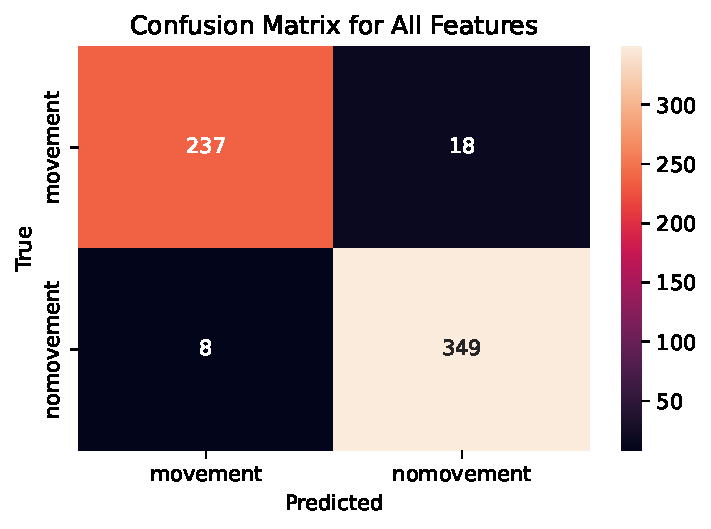
\includegraphics{04_TS_movementAnnotation/02_MovementClassifier_final_files/figure-pdf/cell-4-output-2.pdf}

\section{Head model}\label{head-model}

\begin{Shaded}
\begin{Highlighting}[]
\CommentTok{\# Load head data}
\NormalTok{csv\_path }\OperatorTok{=}\NormalTok{ trainingfolder }\OperatorTok{+} \StringTok{\textquotesingle{}dataset\_head\_mov\_features.csv\textquotesingle{}}

\CommentTok{\# Create a MovementClassifier object}
\NormalTok{model\_head }\OperatorTok{=}\NormalTok{ MovementClassifier(csv\_path)}

\CommentTok{\# load in the model}
\NormalTok{model\_path }\OperatorTok{=}\NormalTok{ modelsfolder }\OperatorTok{+} \StringTok{\textquotesingle{}model\_head\_mov.pkl\textquotesingle{}}
\NormalTok{model\_head }\OperatorTok{=}\NormalTok{ joblib.load(model\_path)}

\CommentTok{\# Load features}
\NormalTok{feature\_indices }\OperatorTok{=} \BuiltInTok{list}\NormalTok{(}\BuiltInTok{range}\NormalTok{(model\_head.df.shape[}\DecValTok{1}\NormalTok{] }\OperatorTok{{-}} \DecValTok{3}\NormalTok{))}

\CommentTok{\# Load the feature and label data}
\NormalTok{X, y }\OperatorTok{=}\NormalTok{ model\_head.load\_and\_process\_data(X\_columns}\OperatorTok{=}\NormalTok{feature\_indices, y\_column}\OperatorTok{=}\StringTok{\textquotesingle{}anno\_value\textquotesingle{}}\NormalTok{)}

\CommentTok{\# Evaluate and plot using the selected features}
\NormalTok{model\_head.evaluate\_and\_plot(}\StringTok{"All"}\NormalTok{, X, y)}

\CommentTok{\# Save the model}
\NormalTok{model\_path }\OperatorTok{=}\NormalTok{ modelsfolder }\OperatorTok{+} \StringTok{\textquotesingle{}model\_head\_mov.pkl\textquotesingle{}}
\NormalTok{joblib.dump(model\_head, model\_path)}
\end{Highlighting}
\end{Shaded}

\begin{verbatim}
This is the evaluation of the model

All Features
Accuracy on training set: 0.9368146214099217
Accuracy on test set: 0.863849765258216
Confusion Matrix
[[243  29]
 [ 58 309]]
Classification Report
              precision    recall  f1-score   support

    movement       0.81      0.89      0.85       272
  nomovement       0.91      0.84      0.88       367

    accuracy                           0.86       639
   macro avg       0.86      0.87      0.86       639
weighted avg       0.87      0.86      0.86       639
\end{verbatim}

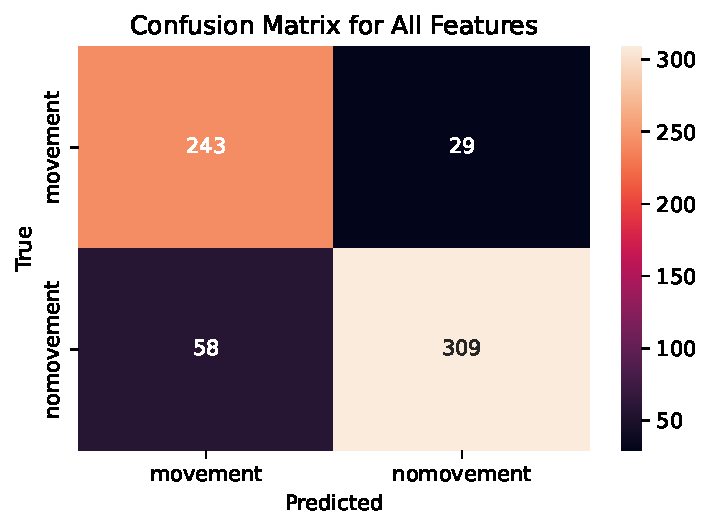
\includegraphics{04_TS_movementAnnotation/02_MovementClassifier_final_files/figure-pdf/cell-5-output-2.pdf}

\section{Upper body model}\label{upper-body-model}

\begin{Shaded}
\begin{Highlighting}[]
\CommentTok{\# Load upper body data}
\NormalTok{csv\_path }\OperatorTok{=}\NormalTok{ trainingfolder }\OperatorTok{+} \StringTok{\textquotesingle{}dataset\_upper\_body\_features.csv\textquotesingle{}}

\CommentTok{\# Create a MovementClassifier object}
\NormalTok{model\_upper }\OperatorTok{=}\NormalTok{ MovementClassifier(csv\_path)}

\CommentTok{\# load in the model}
\NormalTok{model\_path }\OperatorTok{=}\NormalTok{ modelsfolder }\OperatorTok{+} \StringTok{\textquotesingle{}model\_upper\_body.pkl\textquotesingle{}}
\NormalTok{model\_upper }\OperatorTok{=}\NormalTok{ joblib.load(model\_path)}

\CommentTok{\# Load features}
\NormalTok{feature\_indices }\OperatorTok{=} \BuiltInTok{list}\NormalTok{(}\BuiltInTok{range}\NormalTok{(model\_upper.df.shape[}\DecValTok{1}\NormalTok{] }\OperatorTok{{-}} \DecValTok{3}\NormalTok{))}

\CommentTok{\# Load the feature and label data}
\NormalTok{X, y }\OperatorTok{=}\NormalTok{ model\_upper.load\_and\_process\_data(X\_columns}\OperatorTok{=}\NormalTok{feature\_indices, y\_column}\OperatorTok{=}\StringTok{\textquotesingle{}anno\_value\textquotesingle{}}\NormalTok{)}

\CommentTok{\# Evaluate and plot using the selected features}
\NormalTok{model\_upper.evaluate\_and\_plot(}\StringTok{"All"}\NormalTok{, X, y)}

\CommentTok{\# Save the model}
\NormalTok{model\_path }\OperatorTok{=}\NormalTok{ modelsfolder }\OperatorTok{+} \StringTok{\textquotesingle{}model\_upper\_body.pkl\textquotesingle{}}
\NormalTok{joblib.dump(model\_upper, model\_path)}
\end{Highlighting}
\end{Shaded}

\begin{verbatim}
This is the evaluation of the model

All Features
Accuracy on training set: 0.9372409709887507
Accuracy on test set: 0.8632326820603907
Confusion Matrix
[[171  37]
 [ 40 315]]
Classification Report
              precision    recall  f1-score   support

    movement       0.81      0.82      0.82       208
  nomovement       0.89      0.89      0.89       355

    accuracy                           0.86       563
   macro avg       0.85      0.85      0.85       563
weighted avg       0.86      0.86      0.86       563
\end{verbatim}

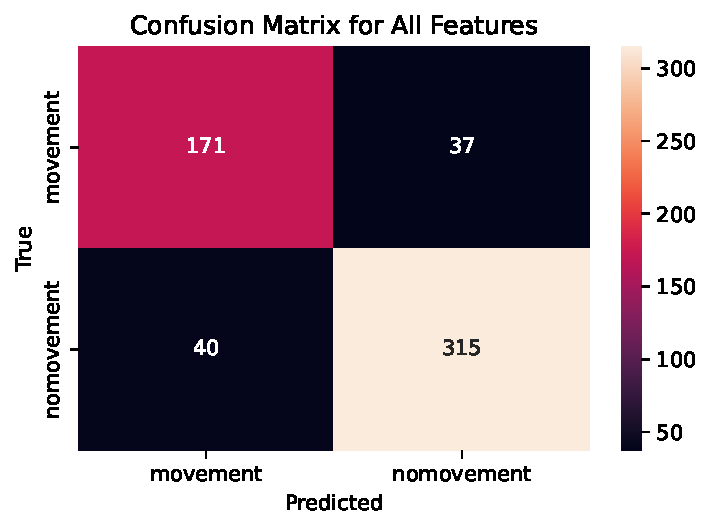
\includegraphics{04_TS_movementAnnotation/02_MovementClassifier_final_files/figure-pdf/cell-6-output-2.pdf}

\section{Lower body model}\label{lower-body-model}

\begin{Shaded}
\begin{Highlighting}[]
\CommentTok{\# Load lower body data}
\NormalTok{csv\_path }\OperatorTok{=}\NormalTok{ trainingfolder }\OperatorTok{+} \StringTok{\textquotesingle{}dataset\_lower\_body\_features.csv\textquotesingle{}}

\CommentTok{\# Create a MovementClassifier object}
\NormalTok{model\_lower }\OperatorTok{=}\NormalTok{ MovementClassifier(csv\_path)}

\CommentTok{\# load in the model}
\NormalTok{model\_path }\OperatorTok{=}\NormalTok{ modelsfolder }\OperatorTok{+} \StringTok{\textquotesingle{}model\_lower\_body.pkl\textquotesingle{}}
\NormalTok{model\_lower }\OperatorTok{=}\NormalTok{ joblib.load(model\_path)}

\CommentTok{\# Load features}
\NormalTok{feature\_indices }\OperatorTok{=} \BuiltInTok{list}\NormalTok{(}\BuiltInTok{range}\NormalTok{(model\_lower.df.shape[}\DecValTok{1}\NormalTok{] }\OperatorTok{{-}} \DecValTok{3}\NormalTok{))}

\CommentTok{\# Load the feature and label data}
\NormalTok{X, y }\OperatorTok{=}\NormalTok{ model\_lower.load\_and\_process\_data(X\_columns}\OperatorTok{=}\NormalTok{feature\_indices, y\_column}\OperatorTok{=}\StringTok{\textquotesingle{}anno\_value\textquotesingle{}}\NormalTok{)}

\CommentTok{\# Evaluate and plot using the selected features}
\NormalTok{model\_lower.evaluate\_and\_plot(}\StringTok{"All"}\NormalTok{, X, y)}

\CommentTok{\# Save the model}
\NormalTok{model\_path }\OperatorTok{=}\NormalTok{ modelsfolder }\OperatorTok{+} \StringTok{\textquotesingle{}model\_lower\_body.pkl\textquotesingle{}}
\NormalTok{joblib.dump(model\_lower, model\_path)}
\end{Highlighting}
\end{Shaded}

\begin{verbatim}
This is the evaluation of the model

All Features
Accuracy on training set: 0.9594921402660218
Accuracy on test set: 0.8913043478260869
Confusion Matrix
[[165  33]
 [ 27 327]]
Classification Report
              precision    recall  f1-score   support

    movement       0.86      0.83      0.85       198
  nomovement       0.91      0.92      0.92       354

    accuracy                           0.89       552
   macro avg       0.88      0.88      0.88       552
weighted avg       0.89      0.89      0.89       552
\end{verbatim}

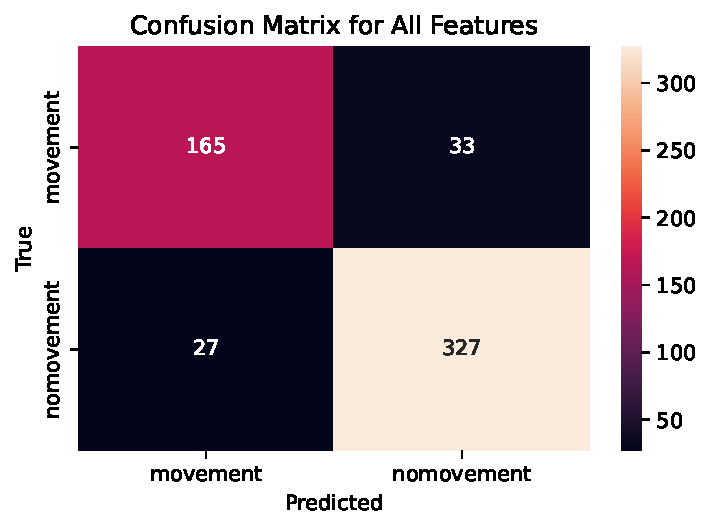
\includegraphics{04_TS_movementAnnotation/02_MovementClassifier_final_files/figure-pdf/cell-7-output-2.pdf}

\bookmarksetup{startatroot}

\chapter{Applying classifier to timeseries
data}\label{applying-classifier-to-timeseries-data}

Now we have trained model to classify a chunk into movement or
no-movement. We will apply the model (per each tier separately) to the
timeseries data that we prepared into consecutive chunks with sliding
step of 25 ms in the previous script ((\textbf{ADDREF?}))

We will also generate a confidence of the model per each chunk, and
average the confidence for overlapping sections to get confidence for a
label as a time-varying signal over the length of each trial.

\begin{Shaded}
\begin{Highlighting}[]
\CommentTok{\# Function to average the confidence values for each time point and create continuous confidence{-}timeline}
\KeywordTok{def}\NormalTok{ generate\_continuous\_timeline(df, max\_time, segment\_duration}\OperatorTok{=}\DecValTok{100}\NormalTok{, shift}\OperatorTok{=}\DecValTok{24}\NormalTok{):}
    \CommentTok{\# Prepare a timeseries of a length equal to the trial duration}
\NormalTok{    timeline }\OperatorTok{=}\NormalTok{ np.arange(}\DecValTok{0}\NormalTok{, max\_time }\OperatorTok{+} \DecValTok{1}\NormalTok{)}

\NormalTok{    continuous\_probabilities }\OperatorTok{=}\NormalTok{ []}

    \CommentTok{\# A loop to calculate the average confidence level at each millisecond:}
    \ControlFlowTok{for}\NormalTok{ t }\KeywordTok{in}\NormalTok{ timeline:}
        \CommentTok{\# Find the segments that overlap with this time point:}
\NormalTok{        overlapping\_segments }\OperatorTok{=}\NormalTok{ df[(df[}\StringTok{\textquotesingle{}start\_time\textquotesingle{}}\NormalTok{] }\OperatorTok{\textless{}=}\NormalTok{ t) }\OperatorTok{\&}\NormalTok{ (df[}\StringTok{\textquotesingle{}start\_time\textquotesingle{}}\NormalTok{] }\OperatorTok{+}\NormalTok{ segment\_duration }\OperatorTok{\textgreater{}}\NormalTok{ t)]}
        
        \CommentTok{\# Average the confidence levels of these overlapping segments}
        \ControlFlowTok{if} \KeywordTok{not}\NormalTok{ overlapping\_segments.empty:}
\NormalTok{            avg\_confidence }\OperatorTok{=}\NormalTok{ overlapping\_segments[}\StringTok{\textquotesingle{}confidence\_movement\textquotesingle{}}\NormalTok{].mean()}
        \ControlFlowTok{else}\NormalTok{:}
\NormalTok{            avg\_confidence }\OperatorTok{=}\NormalTok{ np.nan  }\CommentTok{\# If there is no data at this millisecond}

\NormalTok{        continuous\_probabilities.append(avg\_confidence)}

    \CommentTok{\# Replace the first and last 150 ms of probabilities with zeros to avoid edge bumps (we know anyway there is always a no movement in the beginning and in the end)}
\NormalTok{    change\_duration }\OperatorTok{=} \DecValTok{150}
\NormalTok{    continuous\_probabilities[:change\_duration] }\OperatorTok{=}\NormalTok{ [}\DecValTok{0}\NormalTok{] }\OperatorTok{*}\NormalTok{ change\_duration}
\NormalTok{    continuous\_probabilities[}\OperatorTok{{-}}\NormalTok{change\_duration:] }\OperatorTok{=}\NormalTok{ [}\DecValTok{0}\NormalTok{] }\OperatorTok{*}\NormalTok{ change\_duration}

    \CommentTok{\# Create a df for the continuous probability timeline}
\NormalTok{    continuous\_timeline }\OperatorTok{=}\NormalTok{ pd.DataFrame(\{}\StringTok{\textquotesingle{}time\_ms\textquotesingle{}}\NormalTok{: timeline, }\StringTok{\textquotesingle{}confidence\_movement\textquotesingle{}}\NormalTok{: continuous\_probabilities\})}

    \CommentTok{\# Fill NaN values throughout using forward{-}fill (fill with last value) or backward{-}fill (fill with next value)}
\NormalTok{    continuous\_timeline[}\StringTok{\textquotesingle{}confidence\_movement\textquotesingle{}}\NormalTok{] }\OperatorTok{=}\NormalTok{ continuous\_timeline[}\StringTok{\textquotesingle{}confidence\_movement\textquotesingle{}}\NormalTok{].ffill().bfill()}

    \ControlFlowTok{return}\NormalTok{ continuous\_timeline}

\CommentTok{\# Function to smooth the continuous timeline of confidence scores using a moving average with a fixed window size}
\KeywordTok{def}\NormalTok{ smooth\_timeline(continuous\_timeline, window\_size}\OperatorTok{=}\DecValTok{300}\NormalTok{):}

    \CommentTok{\# Applying smoothing with the specified window size (using ".rolling()" method from pandas)}
    \CommentTok{\# "min\_periods = 1": at least one value in the window should have a value.}
    \CommentTok{\# "center = True": centers the window around the points.}
\NormalTok{    continuous\_timeline[}\StringTok{\textquotesingle{}smoothed\_confidence\textquotesingle{}}\NormalTok{] }\OperatorTok{=}\NormalTok{ continuous\_timeline[}\StringTok{\textquotesingle{}confidence\_movement\textquotesingle{}}\NormalTok{].rolling(window}\OperatorTok{=}\NormalTok{window\_size, min\_periods}\OperatorTok{=}\DecValTok{1}\NormalTok{, center}\OperatorTok{=}\VariableTok{True}\NormalTok{).mean()}
    
    \ControlFlowTok{return}\NormalTok{ continuous\_timeline}
\end{Highlighting}
\end{Shaded}

\begin{Shaded}
\begin{Highlighting}[]
\CommentTok{\# This is were we store the predictions per trial (per tier)}
\NormalTok{predictedfolder }\OperatorTok{=}\NormalTok{ curfolder }\OperatorTok{+} \StringTok{\textquotesingle{}}\CharTok{\textbackslash{}\textbackslash{}}\StringTok{TS\_predicted\_workingfiles}\CharTok{\textbackslash{}\textbackslash{}}\StringTok{\textquotesingle{}}

\CommentTok{\# These are the models we are applying}
\NormalTok{models }\OperatorTok{=}\NormalTok{ [}\StringTok{\textquotesingle{}arms\textquotesingle{}}\NormalTok{, }\StringTok{\textquotesingle{}head\_mov\textquotesingle{}}\NormalTok{, }\StringTok{\textquotesingle{}upper\_body\textquotesingle{}}\NormalTok{, }\StringTok{\textquotesingle{}lower\_body\textquotesingle{}}\NormalTok{]}

\ControlFlowTok{for}\NormalTok{ model }\KeywordTok{in}\NormalTok{ models:}
    \CommentTok{\# Load in the original df}
\NormalTok{    original\_df }\OperatorTok{=}\NormalTok{ pd.read\_csv(trainingfolder }\OperatorTok{+} \SpecialStringTok{f\textquotesingle{}dataset\_}\SpecialCharTok{\{}\NormalTok{model}\SpecialCharTok{\}}\SpecialStringTok{\_features.csv\textquotesingle{}}\NormalTok{)}

    \CommentTok{\# Load in the model}
\NormalTok{    gesture\_model }\OperatorTok{=}\NormalTok{ joblib.load(modelsfolder }\OperatorTok{+} \SpecialStringTok{f\textquotesingle{}model\_}\SpecialCharTok{\{}\NormalTok{model}\SpecialCharTok{\}}\SpecialStringTok{.pkl\textquotesingle{}}\NormalTok{)}

    \CommentTok{\# Loop through each file in the folder...}
    \ControlFlowTok{for}\NormalTok{ filename }\KeywordTok{in}\NormalTok{ os.listdir(classifyingfolder):}
        
        \CommentTok{\# Making sure it\textquotesingle{}s a correct CSV file:}
        \ControlFlowTok{if}\NormalTok{ filename.endswith(}\StringTok{\textquotesingle{}chunked.csv\textquotesingle{}}\NormalTok{):}
            
            \ControlFlowTok{try}\NormalTok{:}
                \CommentTok{\# Load in the chunked timeseries}
\NormalTok{                csv\_path }\OperatorTok{=}\NormalTok{ os.path.join(classifyingfolder, filename)}
\NormalTok{                new\_df }\OperatorTok{=}\NormalTok{ pd.read\_csv(csv\_path)}
                
                \CommentTok{\# This is the max time}
\NormalTok{                max\_time }\OperatorTok{=} \BuiltInTok{int}\NormalTok{(new\_df[}\StringTok{\textquotesingle{}end\_time\textquotesingle{}}\NormalTok{].iloc[}\OperatorTok{{-}}\DecValTok{1}\NormalTok{])}

                \CommentTok{\# Get cols that are in new\_df but not in original\_df {-} otherwise regression model throws an error}
\NormalTok{                extra\_cols }\OperatorTok{=}\NormalTok{ [col }\ControlFlowTok{for}\NormalTok{ col }\KeywordTok{in}\NormalTok{ new\_df.columns }\ControlFlowTok{if}\NormalTok{ col }\KeywordTok{not} \KeywordTok{in}\NormalTok{ original\_df.columns]}

                \CommentTok{\# Create df from new\_df with only the columns that are in original\_df}
\NormalTok{                clean\_df }\OperatorTok{=}\NormalTok{ new\_df[[col }\ControlFlowTok{for}\NormalTok{ col }\KeywordTok{in}\NormalTok{ new\_df.columns }\ControlFlowTok{if}\NormalTok{ col }\KeywordTok{not} \KeywordTok{in}\NormalTok{ extra\_cols]]}

                \CommentTok{\# Reordering df1 columns to match df2}
\NormalTok{                clean\_df\_reordered }\OperatorTok{=}\NormalTok{ new\_df.reindex(columns}\OperatorTok{=}\NormalTok{original\_df.columns)}

                \CommentTok{\# Final clean}
\NormalTok{                clean\_df\_reordered }\OperatorTok{=}\NormalTok{ clean\_df\_reordered.drop(columns}\OperatorTok{=}\NormalTok{[}\StringTok{\textquotesingle{}anno\_value\textquotesingle{}}\NormalTok{])}
\NormalTok{                clean\_df\_reordered }\OperatorTok{=}\NormalTok{ clean\_df\_reordered.iloc[:, :}\OperatorTok{{-}}\DecValTok{2}\NormalTok{]}

                \CommentTok{\# Apply classifier}
\NormalTok{                new\_X }\OperatorTok{=}\NormalTok{ clean\_df\_reordered.values}
\NormalTok{                new\_X }\OperatorTok{=}\NormalTok{ gesture\_model.scaler.transform(new\_X)}
\NormalTok{                new\_X }\OperatorTok{=}\NormalTok{ gesture\_model.min\_max\_scaler.transform(new\_X)}

\NormalTok{                predictions }\OperatorTok{=}\NormalTok{ gesture\_model.model.predict(new\_X)}
\NormalTok{                probabilities }\OperatorTok{=}\NormalTok{ gesture\_model.model.predict\_proba(new\_X)}

\NormalTok{                predicted\_labels }\OperatorTok{=}\NormalTok{ gesture\_model.label\_encoder.inverse\_transform(predictions)}
\NormalTok{                results\_df }\OperatorTok{=}\NormalTok{ pd.DataFrame(\{}
                    \StringTok{\textquotesingle{}start\_time\textquotesingle{}}\NormalTok{: new\_df[}\StringTok{\textquotesingle{}start\_time\textquotesingle{}}\NormalTok{],}
                    \StringTok{\textquotesingle{}predicted\_labels\textquotesingle{}}\NormalTok{: predicted\_labels,}
                    \StringTok{\textquotesingle{}confidence\_movement\textquotesingle{}}\NormalTok{: [prob[}\DecValTok{0}\NormalTok{] }\ControlFlowTok{for}\NormalTok{ prob }\KeywordTok{in}\NormalTok{ probabilities]}
\NormalTok{                \})}

                \CommentTok{\# Generate a continuous timeline}
\NormalTok{                df\_continuous }\OperatorTok{=}\NormalTok{ generate\_continuous\_timeline(results\_df, max\_time)}

                \CommentTok{\# Smooth}
\NormalTok{                df\_smoothed }\OperatorTok{=}\NormalTok{ smooth\_timeline(df\_continuous)}

\NormalTok{                input\_filename }\OperatorTok{=}\NormalTok{ os.path.splitext(filename)[}\DecValTok{0}\NormalTok{]}
\NormalTok{                output\_filename }\OperatorTok{=}\NormalTok{ input\_filename.replace(}\StringTok{\textquotesingle{}chunked\textquotesingle{}}\NormalTok{, }\StringTok{\textquotesingle{}predicted\_smoothed\_confidence.csv\textquotesingle{}}\NormalTok{)}
                \CommentTok{\# Create folder in predictedfolder for model}
                \ControlFlowTok{if} \KeywordTok{not}\NormalTok{ os.path.exists(predictedfolder }\OperatorTok{+} \SpecialStringTok{f\textquotesingle{}}\CharTok{\textbackslash{}\textbackslash{}}\SpecialCharTok{\{}\NormalTok{model}\SpecialCharTok{\}}\CharTok{\textbackslash{}\textbackslash{}}\SpecialStringTok{\textquotesingle{}}\NormalTok{):}
\NormalTok{                    os.makedirs(predictedfolder }\OperatorTok{+} \SpecialStringTok{f\textquotesingle{}}\CharTok{\textbackslash{}\textbackslash{}}\SpecialCharTok{\{}\NormalTok{model}\SpecialCharTok{\}}\CharTok{\textbackslash{}\textbackslash{}}\SpecialStringTok{\textquotesingle{}}\NormalTok{)}
                
                \CommentTok{\# Save it}
\NormalTok{                output\_path }\OperatorTok{=}\NormalTok{ os.path.join(predictedfolder }\OperatorTok{+} \SpecialStringTok{f\textquotesingle{}}\CharTok{\textbackslash{}\textbackslash{}}\SpecialCharTok{\{}\NormalTok{model}\SpecialCharTok{\}}\CharTok{\textbackslash{}\textbackslash{}}\SpecialStringTok{\textquotesingle{}} \OperatorTok{+}\NormalTok{ output\_filename)}
\NormalTok{                df\_smoothed.to\_csv(output\_path, index}\OperatorTok{=}\VariableTok{False}\NormalTok{)}
                \BuiltInTok{print}\NormalTok{(}\SpecialStringTok{f\textquotesingle{}Processed and saved: }\SpecialCharTok{\{}\NormalTok{output\_filename}\SpecialCharTok{\}}\SpecialStringTok{\textquotesingle{}}\NormalTok{)}

            \ControlFlowTok{except} \PreprocessorTok{Exception} \ImportTok{as}\NormalTok{ e:}
                \BuiltInTok{print}\NormalTok{(}\SpecialStringTok{f\textquotesingle{}Error processing file }\SpecialCharTok{\{}\NormalTok{filename}\SpecialCharTok{\}}\SpecialStringTok{: }\SpecialCharTok{\{}\NormalTok{e}\SpecialCharTok{\}}\SpecialStringTok{\textquotesingle{}}\NormalTok{)}
\end{Highlighting}
\end{Shaded}

Now we have each timeseries saved as a variable that states the
confidence of the behaviour being a movement or not (1 is movement, 0 is
no movement). We can see in the plots below how does the confidence look
like on five randomly picked trials.

\begin{Shaded}
\begin{Highlighting}[]
\CommentTok{\# Function to plot confidence}
\KeywordTok{def}\NormalTok{ plot\_smooth\_confidence\_timeline(folder\_path):}

    \ControlFlowTok{try}\NormalTok{:}
        \CommentTok{\# Construct the full path to the file and load the data:}
\NormalTok{        file\_path }\OperatorTok{=}\NormalTok{ os.path.join(folder\_path, filename)}
\NormalTok{        timeline }\OperatorTok{=}\NormalTok{ pd.read\_csv(file\_path)}

        \CommentTok{\# Plot the timeline:}
\NormalTok{        plt.figure(figsize}\OperatorTok{=}\NormalTok{(}\DecValTok{8}\NormalTok{, }\DecValTok{5}\NormalTok{))}
\NormalTok{        plt.plot(timeline[}\StringTok{\textquotesingle{}time\_ms\textquotesingle{}}\NormalTok{], timeline[}\StringTok{\textquotesingle{}confidence\_movement\textquotesingle{}}\NormalTok{], label}\OperatorTok{=}\StringTok{\textquotesingle{}Continuous\textquotesingle{}}\NormalTok{, alpha}\OperatorTok{=}\FloatTok{0.5}\NormalTok{)}
\NormalTok{        plt.plot(timeline[}\StringTok{\textquotesingle{}time\_ms\textquotesingle{}}\NormalTok{], timeline[}\StringTok{\textquotesingle{}smoothed\_confidence\textquotesingle{}}\NormalTok{], label}\OperatorTok{=}\StringTok{\textquotesingle{}Smoothed\textquotesingle{}}\NormalTok{, linewidth}\OperatorTok{=}\DecValTok{2}\NormalTok{)}
        \CommentTok{\# Add red horizontal line at y = 0.8    \# Example threshold 1}
\NormalTok{        plt.axhline(y}\OperatorTok{=}\FloatTok{0.8}\NormalTok{, color}\OperatorTok{=}\StringTok{\textquotesingle{}red\textquotesingle{}}\NormalTok{, linestyle}\OperatorTok{=}\StringTok{\textquotesingle{}{-}{-}\textquotesingle{}}\NormalTok{, linewidth}\OperatorTok{=}\DecValTok{1}\NormalTok{)}
        \CommentTok{\# Add purple horizontal line at y = 0.6    \# Example threshold 2}
\NormalTok{        plt.axhline(y}\OperatorTok{=}\FloatTok{0.6}\NormalTok{, color}\OperatorTok{=}\StringTok{\textquotesingle{}purple\textquotesingle{}}\NormalTok{, linestyle}\OperatorTok{=}\StringTok{\textquotesingle{}{-}{-}\textquotesingle{}}\NormalTok{, linewidth}\OperatorTok{=}\DecValTok{1}\NormalTok{)}
\NormalTok{        plt.xlabel(}\StringTok{\textquotesingle{}Time (ms)\textquotesingle{}}\NormalTok{)}
\NormalTok{        plt.ylabel(}\StringTok{\textquotesingle{}Confidence Movement Probability\textquotesingle{}}\NormalTok{)}
\NormalTok{        plt.ylim(}\DecValTok{0}\NormalTok{, }\FloatTok{1.1}\NormalTok{)  }\CommentTok{\# Set y{-}axis limits between 0 and 1.1 for better visualization }
\NormalTok{        plt.legend()}
\NormalTok{        plt.title(}\SpecialStringTok{f\textquotesingle{}File: }\SpecialCharTok{\{}\NormalTok{filename}\SpecialCharTok{.}\NormalTok{split(}\StringTok{\textquotesingle{}}\CharTok{\textbackslash{}\textbackslash{}}\StringTok{\textquotesingle{}}\NormalTok{)[}\OperatorTok{{-}}\DecValTok{1}\NormalTok{]}\SpecialCharTok{\}}\SpecialStringTok{\textquotesingle{}}\NormalTok{)}
\NormalTok{        plt.show()}

    \ControlFlowTok{except} \PreprocessorTok{Exception} \ImportTok{as}\NormalTok{ e:}
        \BuiltInTok{print}\NormalTok{(}\SpecialStringTok{f\textquotesingle{}Error processing file }\SpecialCharTok{\{}\NormalTok{filename}\SpecialCharTok{\}}\SpecialStringTok{: }\SpecialCharTok{\{}\NormalTok{e}\SpecialCharTok{\}}\SpecialStringTok{\textquotesingle{}}\NormalTok{)}
\end{Highlighting}
\end{Shaded}

\includegraphics{04_TS_movementAnnotation/02_MovementClassifier_final_files/figure-pdf/cell-11-output-1.pdf}

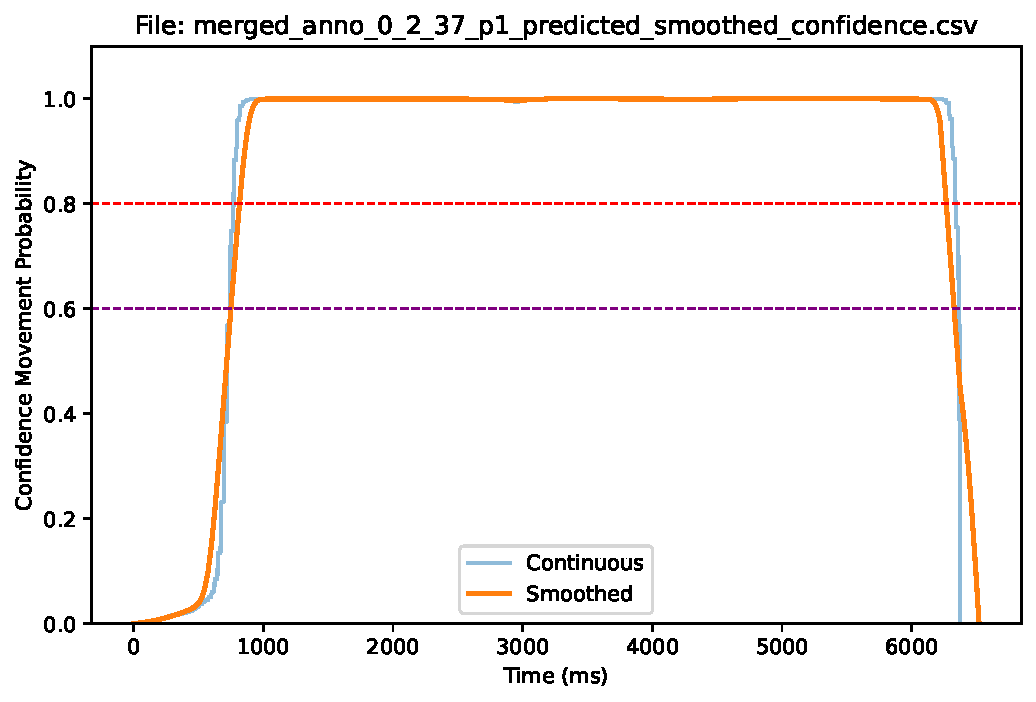
\includegraphics{04_TS_movementAnnotation/02_MovementClassifier_final_files/figure-pdf/cell-11-output-2.pdf}

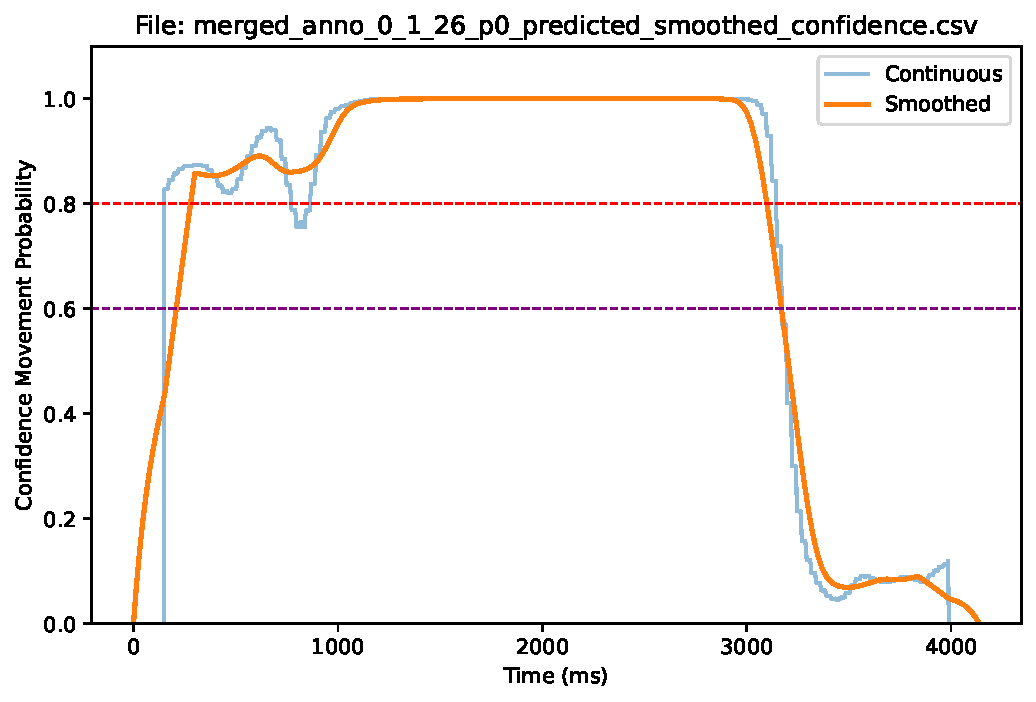
\includegraphics{04_TS_movementAnnotation/02_MovementClassifier_final_files/figure-pdf/cell-11-output-3.pdf}

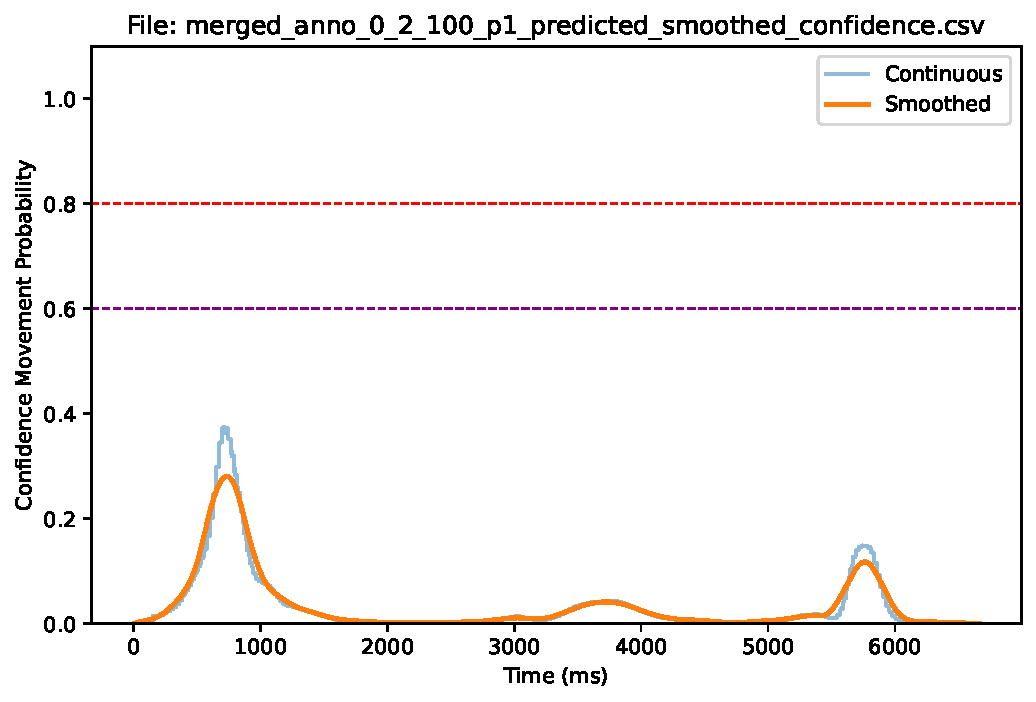
\includegraphics{04_TS_movementAnnotation/02_MovementClassifier_final_files/figure-pdf/cell-11-output-4.pdf}

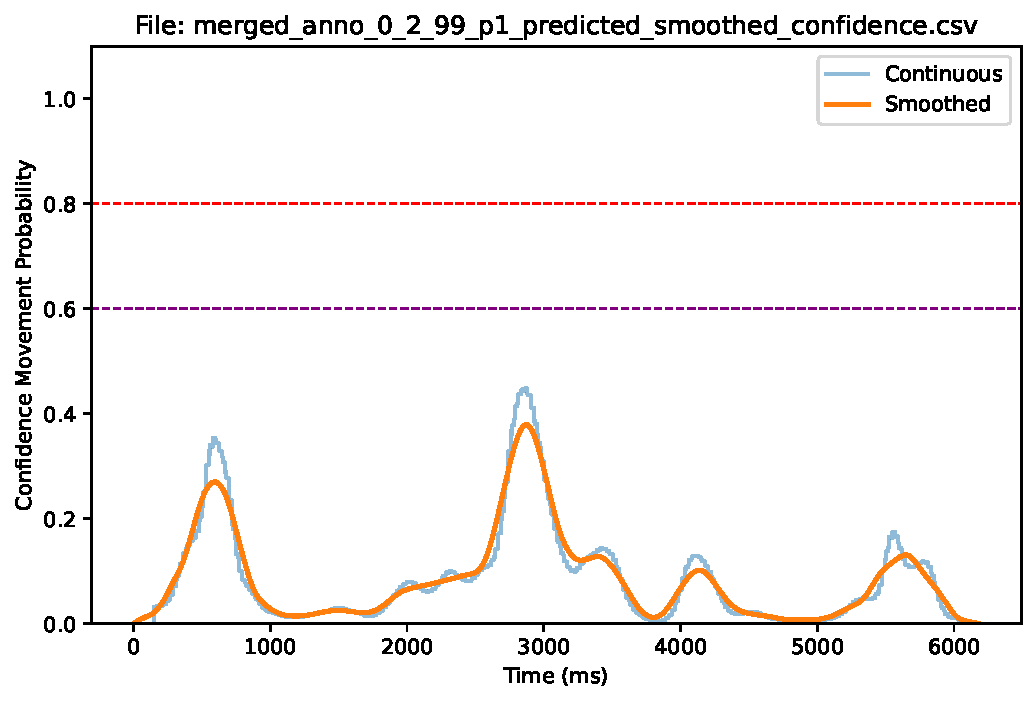
\includegraphics{04_TS_movementAnnotation/02_MovementClassifier_final_files/figure-pdf/cell-11-output-5.pdf}

We can check back to the original videos how does the predictions fit to
the actual occurence of movement in trial. We can now set a threshold to
determine which confidence level is enough to say that movement is
present. We will try two different threshold - 60\% and 80\% - to test
the sensitivity of the model, and compare the annotations created with
these two thresholds against the manual annotations (see next script
(\textbf{ADDREF?})).

\begin{Shaded}
\begin{Highlighting}[]
\CommentTok{\# Function to annotate trials based on the confidence threshold}
\KeywordTok{def}\NormalTok{ annotate\_files(tier, folder\_path, annotated\_path, threshold):}
    \CommentTok{\# Create a new folder path based on the threshold value}
\NormalTok{    threshold\_str }\OperatorTok{=} \SpecialStringTok{f"}\SpecialCharTok{\{}\NormalTok{threshold}\SpecialCharTok{\}}\SpecialStringTok{"}\NormalTok{.replace(}\StringTok{"."}\NormalTok{, }\StringTok{"\_"}\NormalTok{)  }
\NormalTok{    new\_foldername }\OperatorTok{=} \SpecialStringTok{f"}\SpecialCharTok{\{}\NormalTok{tier}\SpecialCharTok{\}}\SpecialStringTok{\_annotations\_threshold\_}\SpecialCharTok{\{}\NormalTok{threshold\_str}\SpecialCharTok{\}}\SpecialStringTok{"} 
\NormalTok{    new\_folder\_path }\OperatorTok{=}\NormalTok{ os.path.join(annotated\_path, new\_foldername)}

    \CommentTok{\# Create the new folder in annotated path}
    \ControlFlowTok{if} \KeywordTok{not}\NormalTok{ os.path.exists(new\_folder\_path):}
\NormalTok{        os.makedirs(new\_folder\_path)}

\NormalTok{    files }\OperatorTok{=}\NormalTok{ glob.glob(folder\_path }\OperatorTok{+} \StringTok{\textquotesingle{}*.csv\textquotesingle{}}\NormalTok{)}

    \ControlFlowTok{for}\NormalTok{ filename }\KeywordTok{in}\NormalTok{ files:}
        \ControlFlowTok{if}\NormalTok{ filename.endswith(}\StringTok{"smoothed\_confidence.csv"}\NormalTok{): }
            \BuiltInTok{print}\NormalTok{(}\SpecialStringTok{f"Processing file: }\SpecialCharTok{\{}\NormalTok{filename}\SpecialCharTok{\}}\SpecialStringTok{"}\NormalTok{)}
\NormalTok{            file\_path }\OperatorTok{=}\NormalTok{ os.path.join(folder\_path, filename)}
\NormalTok{            filename }\OperatorTok{=}\NormalTok{ os.path.basename(file\_path)}

            \CommentTok{\# Load the CSV file}
\NormalTok{            df }\OperatorTok{=}\NormalTok{ pd.read\_csv(file\_path)}
            
            \CommentTok{\# Add an \textquotesingle{}anno\_values\textquotesingle{} column with annotations based on \textquotesingle{}smoothed\_confidence\textquotesingle{} values and threshold}
\NormalTok{            df[}\StringTok{\textquotesingle{}anno\_values\textquotesingle{}}\NormalTok{] }\OperatorTok{=}\NormalTok{ df[}\StringTok{\textquotesingle{}smoothed\_confidence\textquotesingle{}}\NormalTok{].}\BuiltInTok{apply}\NormalTok{(}\KeywordTok{lambda}\NormalTok{ x: }\StringTok{\textquotesingle{}movement\textquotesingle{}} \ControlFlowTok{if}\NormalTok{ x }\OperatorTok{\textgreater{}}\NormalTok{ threshold }\ControlFlowTok{else} \StringTok{\textquotesingle{}no movement\textquotesingle{}}\NormalTok{)}
            
            \CommentTok{\# Create a new file}
\NormalTok{            new\_filename }\OperatorTok{=}\NormalTok{ filename.replace(}\StringTok{"predicted\_smoothed\_confidence.csv"}\NormalTok{, }\SpecialStringTok{f"annotated\_threshold\_}\SpecialCharTok{\{}\NormalTok{threshold\_str}\SpecialCharTok{\}}\SpecialStringTok{.csv"}\NormalTok{)}
\NormalTok{            output\_path }\OperatorTok{=}\NormalTok{ os.path.join(new\_folder\_path, new\_filename)}
            
            \CommentTok{\# Save it}
\NormalTok{            df.to\_csv(output\_path, index}\OperatorTok{=}\VariableTok{False}\NormalTok{)}
\end{Highlighting}
\end{Shaded}

\begin{Shaded}
\begin{Highlighting}[]
\CommentTok{\# Here we store the predicted values with confidence per trial (and tier)}
\NormalTok{folder\_path }\OperatorTok{=}\NormalTok{ curfolder }\OperatorTok{+} \StringTok{\textquotesingle{}}\CharTok{\textbackslash{}\textbackslash{}}\StringTok{TS\_predicted\_workingfiles}\CharTok{\textbackslash{}\textbackslash{}}\StringTok{\textquotesingle{}}
\CommentTok{\# Here we store the trials annotated by the model}
\NormalTok{annotated\_path }\OperatorTok{=}\NormalTok{ curfolder }\OperatorTok{+} \StringTok{\textquotesingle{}}\CharTok{\textbackslash{}\textbackslash{}}\StringTok{TS\_annotated\_logreg}\CharTok{\textbackslash{}\textbackslash{}}\StringTok{\textquotesingle{}}

\NormalTok{tiers }\OperatorTok{=}\NormalTok{ [}\StringTok{\textquotesingle{}arms\textquotesingle{}}\NormalTok{, }\StringTok{\textquotesingle{}head\_mov\textquotesingle{}}\NormalTok{, }\StringTok{\textquotesingle{}upper\_body\textquotesingle{}}\NormalTok{, }\StringTok{\textquotesingle{}lower\_body\textquotesingle{}}\NormalTok{]}

\ControlFlowTok{for}\NormalTok{ tier }\KeywordTok{in}\NormalTok{ tiers:}
\NormalTok{    folder\_path\_tier }\OperatorTok{=}\NormalTok{ folder\_path }\OperatorTok{+} \SpecialStringTok{f\textquotesingle{}}\SpecialCharTok{\{}\NormalTok{tier}\SpecialCharTok{\}}\CharTok{\textbackslash{}\textbackslash{}}\SpecialStringTok{\textquotesingle{}}

    \CommentTok{\# Annotate with threshold 60\%}
\NormalTok{    threshold }\OperatorTok{=} \FloatTok{0.6}
\NormalTok{    annotate\_files(tier, folder\_path\_tier, annotated\_path, threshold)}

    \CommentTok{\# Annotate with threshold 80\%}
\NormalTok{    threshold }\OperatorTok{=} \FloatTok{0.8}
\NormalTok{    annotate\_files(tier, folder\_path\_tier, annotated\_path, threshold)}
\end{Highlighting}
\end{Shaded}

Below, you can see how now each trial looks like in terms of the
movement annotated by the model on five randomly picked files.

\begin{Shaded}
\begin{Highlighting}[]
\CommentTok{\# Function to plot annotated trial}
\KeywordTok{def}\NormalTok{ plot\_movement\_timeline(folder\_path, filename):}
\NormalTok{    file\_path }\OperatorTok{=}\NormalTok{ os.path.join(folder\_path, filename)}
\NormalTok{    df }\OperatorTok{=}\NormalTok{ pd.read\_csv(file\_path)}

    \ControlFlowTok{if} \StringTok{\textquotesingle{}time\_ms\textquotesingle{}} \KeywordTok{not} \KeywordTok{in}\NormalTok{ df.columns }\KeywordTok{or} \StringTok{\textquotesingle{}anno\_values\textquotesingle{}} \KeywordTok{not} \KeywordTok{in}\NormalTok{ df.columns:}
        \BuiltInTok{print}\NormalTok{(}\SpecialStringTok{f"Error: Required columns missing in }\SpecialCharTok{\{}\NormalTok{filename}\SpecialCharTok{\}}\SpecialStringTok{"}\NormalTok{)}
        \ControlFlowTok{return}

\NormalTok{    df[}\StringTok{\textquotesingle{}movement\_binary\textquotesingle{}}\NormalTok{] }\OperatorTok{=}\NormalTok{ df[}\StringTok{\textquotesingle{}anno\_values\textquotesingle{}}\NormalTok{].}\BuiltInTok{apply}\NormalTok{(}\KeywordTok{lambda}\NormalTok{ x: }\DecValTok{1} \ControlFlowTok{if}\NormalTok{ x }\OperatorTok{==} \StringTok{"movement"} \ControlFlowTok{else} \DecValTok{0}\NormalTok{)}

    \CommentTok{\# Convert columns to numeric}
\NormalTok{    df[}\StringTok{\textquotesingle{}time\_ms\textquotesingle{}}\NormalTok{] }\OperatorTok{=}\NormalTok{ pd.to\_numeric(df[}\StringTok{\textquotesingle{}time\_ms\textquotesingle{}}\NormalTok{], errors}\OperatorTok{=}\StringTok{\textquotesingle{}coerce\textquotesingle{}}\NormalTok{)}
\NormalTok{    df[}\StringTok{\textquotesingle{}movement\_binary\textquotesingle{}}\NormalTok{] }\OperatorTok{=}\NormalTok{ pd.to\_numeric(df[}\StringTok{\textquotesingle{}movement\_binary\textquotesingle{}}\NormalTok{], errors}\OperatorTok{=}\StringTok{\textquotesingle{}coerce\textquotesingle{}}\NormalTok{)}

    \CommentTok{\# Drop NaN rows}
\NormalTok{    df.dropna(subset}\OperatorTok{=}\NormalTok{[}\StringTok{\textquotesingle{}time\_ms\textquotesingle{}}\NormalTok{, }\StringTok{\textquotesingle{}movement\_binary\textquotesingle{}}\NormalTok{], inplace}\OperatorTok{=}\VariableTok{True}\NormalTok{)}

    \CommentTok{\# Plot}
\NormalTok{    plt.figure(figsize}\OperatorTok{=}\NormalTok{(}\DecValTok{8}\NormalTok{, }\DecValTok{3}\NormalTok{))}
\NormalTok{    plt.plot(df[}\StringTok{\textquotesingle{}time\_ms\textquotesingle{}}\NormalTok{], df[}\StringTok{\textquotesingle{}movement\_binary\textquotesingle{}}\NormalTok{], color}\OperatorTok{=}\StringTok{"orange"}\NormalTok{, linewidth}\OperatorTok{=}\DecValTok{2}\NormalTok{)}
\NormalTok{    plt.fill\_between(df[}\StringTok{\textquotesingle{}time\_ms\textquotesingle{}}\NormalTok{], df[}\StringTok{\textquotesingle{}movement\_binary\textquotesingle{}}\NormalTok{], color}\OperatorTok{=}\StringTok{"orange"}\NormalTok{, alpha}\OperatorTok{=}\FloatTok{0.3}\NormalTok{, label}\OperatorTok{=}\StringTok{"Movement"}\NormalTok{)}
    
\NormalTok{    plt.yticks([}\DecValTok{0}\NormalTok{, }\DecValTok{1}\NormalTok{], [}\StringTok{\textquotesingle{}No Movement\textquotesingle{}}\NormalTok{, }\StringTok{\textquotesingle{}Movement\textquotesingle{}}\NormalTok{])}
\NormalTok{    plt.xlabel(}\StringTok{"Time (ms)"}\NormalTok{)}
\NormalTok{    plt.title(}\StringTok{"Movement Timeline"}\NormalTok{)}
\NormalTok{    plt.title(}\SpecialStringTok{f\textquotesingle{}File: }\SpecialCharTok{\{}\NormalTok{filename}\SpecialCharTok{.}\NormalTok{split(}\StringTok{\textquotesingle{}}\CharTok{\textbackslash{}\textbackslash{}}\StringTok{\textquotesingle{}}\NormalTok{)[}\OperatorTok{{-}}\DecValTok{1}\NormalTok{]}\SpecialCharTok{\}}\SpecialStringTok{\textquotesingle{}}\NormalTok{)}
\NormalTok{    plt.legend()}
\NormalTok{    plt.show()}
\end{Highlighting}
\end{Shaded}

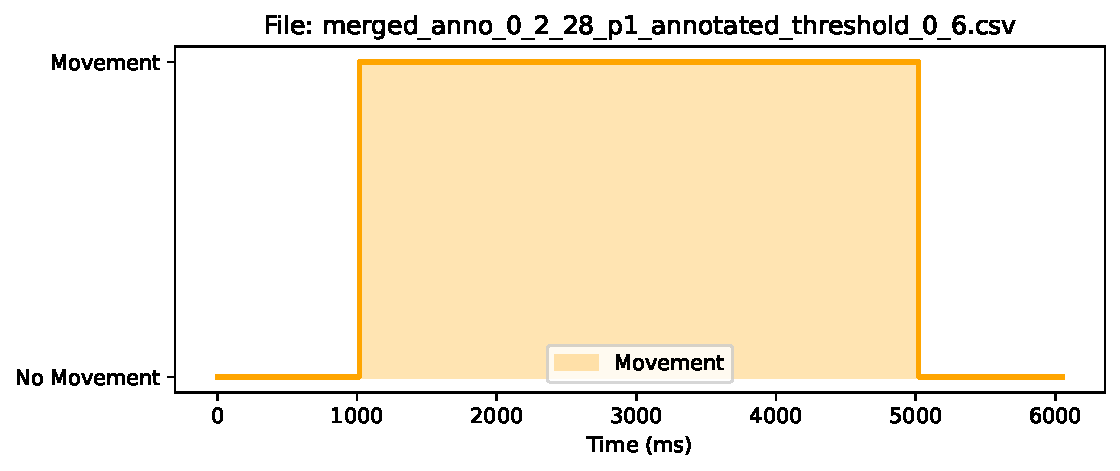
\includegraphics{04_TS_movementAnnotation/02_MovementClassifier_final_files/figure-pdf/cell-15-output-1.pdf}

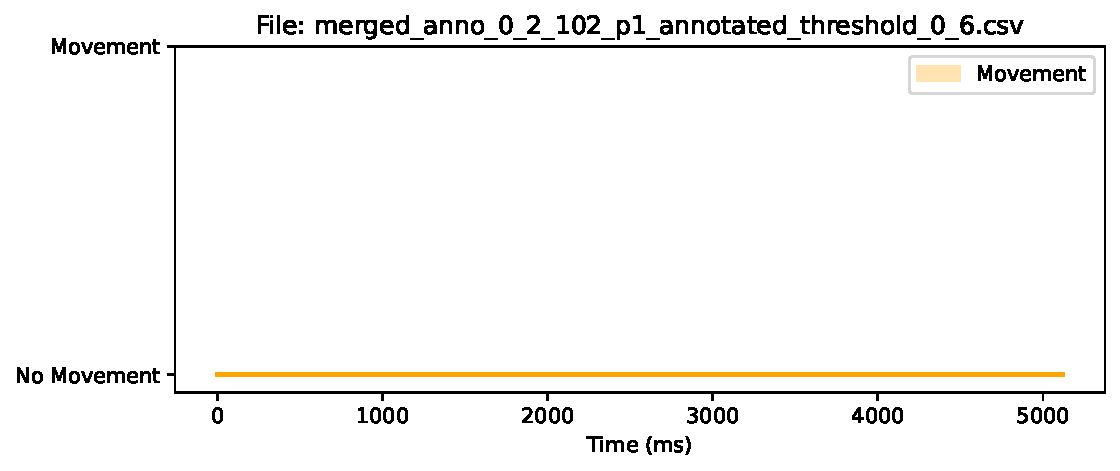
\includegraphics{04_TS_movementAnnotation/02_MovementClassifier_final_files/figure-pdf/cell-15-output-2.pdf}

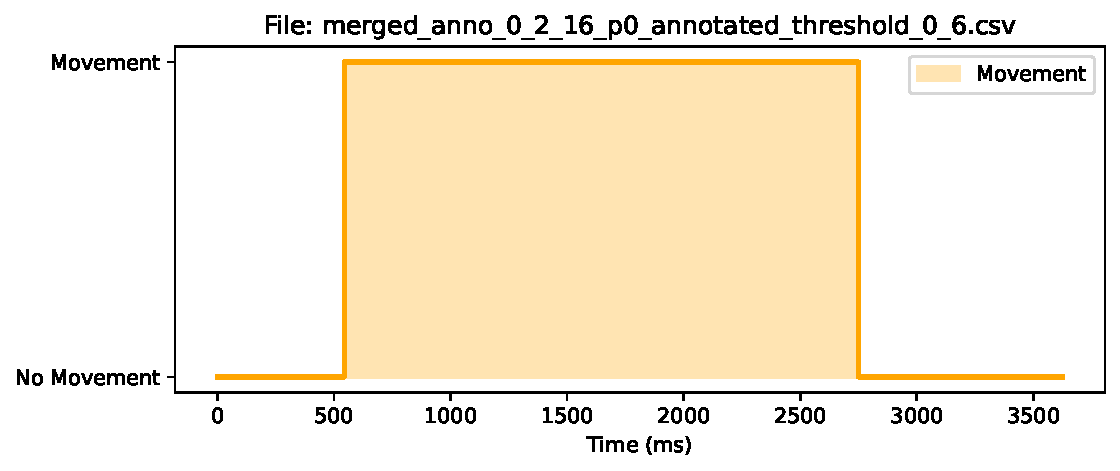
\includegraphics{04_TS_movementAnnotation/02_MovementClassifier_final_files/figure-pdf/cell-15-output-3.pdf}

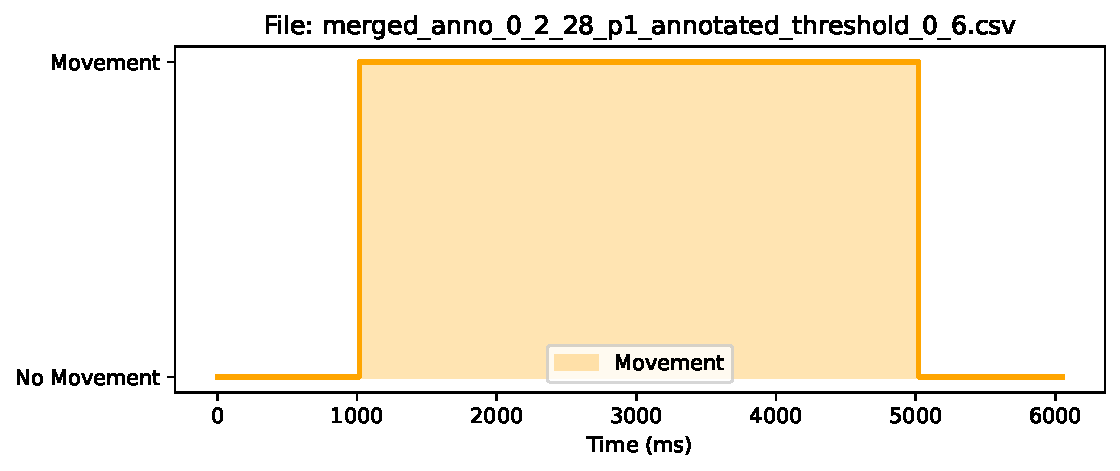
\includegraphics{04_TS_movementAnnotation/02_MovementClassifier_final_files/figure-pdf/cell-15-output-4.pdf}

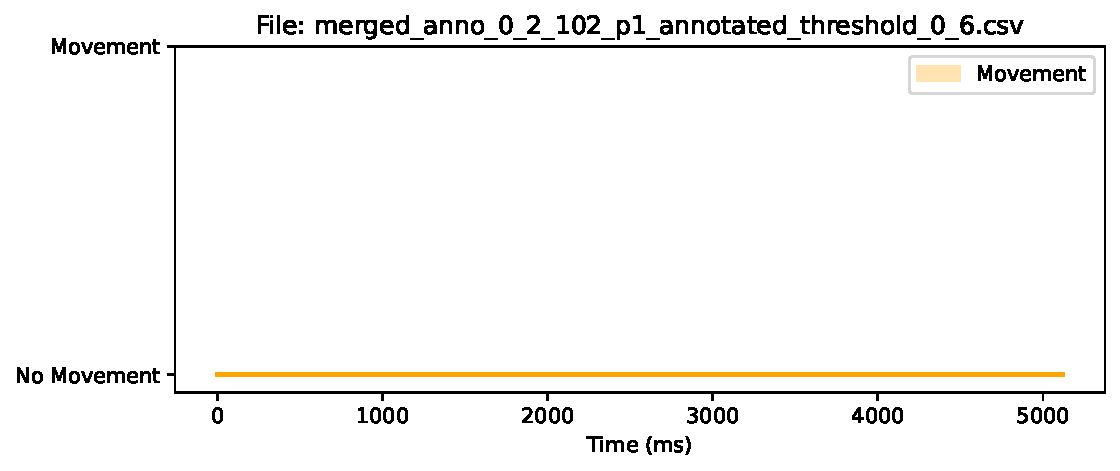
\includegraphics{04_TS_movementAnnotation/02_MovementClassifier_final_files/figure-pdf/cell-15-output-5.pdf}

In the following script (\textbf{ADDREF?}), we will compare the
annotations created by the model (with both confidence thresholds)
against the manual annotations in order to (1) validate the automatic
annotations, and (2) decide which threshold to use for the final
annotations.

\bookmarksetup{startatroot}

\chapter{Movement annotation III: Testing the interrater agreement
between manual and automatic
annotation}\label{movement-annotation-iii-testing-the-interrater-agreement-between-manual-and-automatic-annotation}

In this script, we prepare data to test the interrater agreement (IA) on
movement annotation. To test the robustness, we compute interrater
agreement between two human annotators (AC, GR) and between each human
annotator and the automatic annotation created in the previous script
((\textbf{ADDREF?})). We compute IA for each tier separately.

We use EasyDIAG ((\textbf{holle\_rein15?})) to compute the IA, but
document the results here in the table.

\begin{Shaded}
\begin{Highlighting}[]
\ImportTok{import}\NormalTok{ os}
\ImportTok{import}\NormalTok{ glob}
\ImportTok{import}\NormalTok{ numpy }\ImportTok{as}\NormalTok{ np}
\ImportTok{import}\NormalTok{ pandas }\ImportTok{as}\NormalTok{ pd}
\ImportTok{import}\NormalTok{ xml.etree.ElementTree }\ImportTok{as}\NormalTok{ ET}

\NormalTok{curfolder }\OperatorTok{=}\NormalTok{ os.getcwd()}

\CommentTok{\# Here we store our merged processed files}
\NormalTok{processedfolder }\OperatorTok{=}\NormalTok{ os.path.join(curfolder }\OperatorTok{+} \StringTok{\textquotesingle{}}\CharTok{\textbackslash{}\textbackslash{}}\StringTok{..}\CharTok{\textbackslash{}\textbackslash{}}\StringTok{03\_TS\_processing}\CharTok{\textbackslash{}\textbackslash{}}\StringTok{TS\_merged}\CharTok{\textbackslash{}\textbackslash{}}\StringTok{\textquotesingle{}}\NormalTok{)}
\NormalTok{processedfiles }\OperatorTok{=}\NormalTok{ glob.glob(processedfolder }\OperatorTok{+} \StringTok{\textquotesingle{}*.csv\textquotesingle{}}\NormalTok{)}

\CommentTok{\# Here we store annotations from the logreg model}
\NormalTok{annotatedfolder }\OperatorTok{=}\NormalTok{ os.path.join(curfolder }\OperatorTok{+} \StringTok{\textquotesingle{}}\CharTok{\textbackslash{}\textbackslash{}}\StringTok{TS\_annotated\_logreg}\CharTok{\textbackslash{}\textbackslash{}}\StringTok{\textquotesingle{}}\NormalTok{)}
\NormalTok{folders }\OperatorTok{=}\NormalTok{ glob.glob(annotatedfolder }\OperatorTok{+} \StringTok{\textquotesingle{}*}\CharTok{\textbackslash{}\textbackslash{}}\StringTok{\textquotesingle{}}\NormalTok{)}

\NormalTok{folders60 }\OperatorTok{=}\NormalTok{ [x }\ControlFlowTok{for}\NormalTok{ x }\KeywordTok{in}\NormalTok{ folders }\ControlFlowTok{if} \StringTok{\textquotesingle{}0\_6\textquotesingle{}} \KeywordTok{in}\NormalTok{ x] }\CommentTok{\#60percent confidence}
\NormalTok{folders80 }\OperatorTok{=}\NormalTok{ [x }\ControlFlowTok{for}\NormalTok{ x }\KeywordTok{in}\NormalTok{ folders }\ControlFlowTok{if} \StringTok{\textquotesingle{}0\_8\textquotesingle{}} \KeywordTok{in}\NormalTok{ x] }\CommentTok{\#80percent confidence}

\CommentTok{\# Here we store manual annotations from R1 (AC)}
\NormalTok{manualfolder1 }\OperatorTok{=}\NormalTok{ os.path.join(curfolder }\OperatorTok{+} \StringTok{\textquotesingle{}}\CharTok{\textbackslash{}\textbackslash{}}\StringTok{ManualAnno}\CharTok{\textbackslash{}\textbackslash{}}\StringTok{R1}\CharTok{\textbackslash{}\textbackslash{}}\StringTok{\textquotesingle{}}\NormalTok{)}
\NormalTok{manualfiles1 }\OperatorTok{=}\NormalTok{ glob.glob(manualfolder1 }\OperatorTok{+} \StringTok{\textquotesingle{}*.eaf\textquotesingle{}}\NormalTok{)}
\NormalTok{manualfiles1 }\OperatorTok{=}\NormalTok{ [x }\ControlFlowTok{for}\NormalTok{ x }\KeywordTok{in}\NormalTok{ manualfiles1 }\ControlFlowTok{if} \StringTok{\textquotesingle{}ELAN\_tiers\textquotesingle{}} \KeywordTok{in}\NormalTok{ x]}

\CommentTok{\# Here we store manual annotations from R2 (GR)}
\NormalTok{manualfolder2 }\OperatorTok{=}\NormalTok{ os.path.join(curfolder }\OperatorTok{+} \StringTok{\textquotesingle{}}\CharTok{\textbackslash{}\textbackslash{}}\StringTok{ManualAnno}\CharTok{\textbackslash{}\textbackslash{}}\StringTok{R3}\CharTok{\textbackslash{}\textbackslash{}}\StringTok{\textquotesingle{}}\NormalTok{)}
\NormalTok{manualfiles2 }\OperatorTok{=}\NormalTok{ glob.glob(manualfolder2 }\OperatorTok{+} \StringTok{\textquotesingle{}*.eaf\textquotesingle{}}\NormalTok{)}
\NormalTok{manualfiles2 }\OperatorTok{=}\NormalTok{ [x }\ControlFlowTok{for}\NormalTok{ x }\KeywordTok{in}\NormalTok{ manualfiles2 }\ControlFlowTok{if} \StringTok{\textquotesingle{}ELAN\_tiers\textquotesingle{}} \KeywordTok{in}\NormalTok{ x]}

\CommentTok{\# Here we store the txt files we need for EasyDIAG}
\NormalTok{interfolder }\OperatorTok{=}\NormalTok{ curfolder }\OperatorTok{+} \StringTok{\textquotesingle{}}\CharTok{\textbackslash{}\textbackslash{}}\StringTok{InterAg}\CharTok{\textbackslash{}\textbackslash{}}\StringTok{\textquotesingle{}}
\end{Highlighting}
\end{Shaded}

\bookmarksetup{startatroot}

\chapter{Preprocessing annotations}\label{preprocessing-annotations}

Now we need to get both manual and automatic annotations into format
that EasyDIAG requires - so simple .txt files with timestamps and
annotation values. For annotations that have been created by human
annotators, we need to extract the timestamps and values from the .eaf
files.

\begin{Shaded}
\begin{Highlighting}[]
\CommentTok{\# Function to parse ELAN file}
\KeywordTok{def}\NormalTok{ parse\_eaf\_file(eaf\_file, rel\_tiers):}
\NormalTok{    tree }\OperatorTok{=}\NormalTok{ ET.parse(eaf\_file)}
\NormalTok{    root }\OperatorTok{=}\NormalTok{ tree.getroot()}

\NormalTok{    time\_order }\OperatorTok{=}\NormalTok{ root.find(}\StringTok{\textquotesingle{}TIME\_ORDER\textquotesingle{}}\NormalTok{)}
\NormalTok{    time\_slots }\OperatorTok{=}\NormalTok{ \{time\_slot.attrib[}\StringTok{\textquotesingle{}TIME\_SLOT\_ID\textquotesingle{}}\NormalTok{]: time\_slot.attrib[}\StringTok{\textquotesingle{}TIME\_VALUE\textquotesingle{}}\NormalTok{] }\ControlFlowTok{for}\NormalTok{ time\_slot }\KeywordTok{in}\NormalTok{ time\_order\}}

\NormalTok{    annotations }\OperatorTok{=}\NormalTok{ []}
\NormalTok{    relevant\_tiers }\OperatorTok{=}\NormalTok{ \{rel\_tiers\}}
    \ControlFlowTok{for}\NormalTok{ tier }\KeywordTok{in}\NormalTok{ root.findall(}\StringTok{\textquotesingle{}TIER\textquotesingle{}}\NormalTok{):}
\NormalTok{        tier\_id }\OperatorTok{=}\NormalTok{ tier.attrib[}\StringTok{\textquotesingle{}TIER\_ID\textquotesingle{}}\NormalTok{]}
        \ControlFlowTok{if}\NormalTok{ tier\_id }\KeywordTok{in}\NormalTok{ relevant\_tiers:}
            \ControlFlowTok{for}\NormalTok{ annotation }\KeywordTok{in}\NormalTok{ tier.findall(}\StringTok{\textquotesingle{}ANNOTATION/ALIGNABLE\_ANNOTATION\textquotesingle{}}\NormalTok{):}
                \CommentTok{\# Ensure required attributes are present}
                \ControlFlowTok{if} \StringTok{\textquotesingle{}TIME\_SLOT\_REF1\textquotesingle{}} \KeywordTok{in}\NormalTok{ annotation.attrib }\KeywordTok{and} \StringTok{\textquotesingle{}TIME\_SLOT\_REF2\textquotesingle{}} \KeywordTok{in}\NormalTok{ annotation.attrib:}
\NormalTok{                    ts\_ref1 }\OperatorTok{=}\NormalTok{ annotation.attrib[}\StringTok{\textquotesingle{}TIME\_SLOT\_REF1\textquotesingle{}}\NormalTok{]}
\NormalTok{                    ts\_ref2 }\OperatorTok{=}\NormalTok{ annotation.attrib[}\StringTok{\textquotesingle{}TIME\_SLOT\_REF2\textquotesingle{}}\NormalTok{]}
                    \CommentTok{\# Get annotation ID if it exists, otherwise set to None}
\NormalTok{                    ann\_id }\OperatorTok{=}\NormalTok{ annotation.attrib.get(}\StringTok{\textquotesingle{}ANNOTATION\_ID\textquotesingle{}}\NormalTok{, }\VariableTok{None}\NormalTok{)}
\NormalTok{                    annotation\_value }\OperatorTok{=}\NormalTok{ annotation.find(}\StringTok{\textquotesingle{}ANNOTATION\_VALUE\textquotesingle{}}\NormalTok{).text.strip()}
\NormalTok{                    annotations.append(\{}
                        \StringTok{\textquotesingle{}tier\_id\textquotesingle{}}\NormalTok{: tier\_id,}
                        \StringTok{\textquotesingle{}annotation\_id\textquotesingle{}}\NormalTok{: ann\_id,}
                        \StringTok{\textquotesingle{}start\_time\textquotesingle{}}\NormalTok{: time\_slots[ts\_ref1],}
                        \StringTok{\textquotesingle{}end\_time\textquotesingle{}}\NormalTok{: time\_slots[ts\_ref2],}
                        \StringTok{\textquotesingle{}annotation\_value\textquotesingle{}}\NormalTok{: annotation\_value}
\NormalTok{                    \})}

    \ControlFlowTok{return}\NormalTok{ annotations}

\CommentTok{\# Function to write ELAN into txt file}
\KeywordTok{def}\NormalTok{ ELAN\_into\_txt(txtfile, raterID, foi, tier):}
    \ControlFlowTok{with} \BuiltInTok{open}\NormalTok{(txtfile, }\StringTok{\textquotesingle{}w\textquotesingle{}}\NormalTok{) }\ImportTok{as}\NormalTok{ f:}
        \ControlFlowTok{for} \BuiltInTok{file} \KeywordTok{in}\NormalTok{ foi:}
            \BuiltInTok{print}\NormalTok{(}\StringTok{\textquotesingle{}working on \textquotesingle{}} \OperatorTok{+} \BuiltInTok{file}\NormalTok{)}
            \CommentTok{\# Filename}
\NormalTok{            filename }\OperatorTok{=} \BuiltInTok{file}\NormalTok{.split(}\StringTok{\textquotesingle{}}\CharTok{\textbackslash{}\textbackslash{}}\StringTok{\textquotesingle{}}\NormalTok{)[}\OperatorTok{{-}}\DecValTok{1}\NormalTok{]}
            \CommentTok{\# Parse ELAN file}
\NormalTok{            annotations }\OperatorTok{=}\NormalTok{ parse\_eaf\_file(}\BuiltInTok{file}\NormalTok{, tier)}
            \CommentTok{\# Write annotations into txt file}
            \ControlFlowTok{for}\NormalTok{ annotation }\KeywordTok{in}\NormalTok{ annotations:}
\NormalTok{                f.write(}\SpecialStringTok{f"Anno\_}\SpecialCharTok{\{}\NormalTok{raterID}\SpecialCharTok{\}}\CharTok{\textbackslash{}t}\SpecialCharTok{\{}\NormalTok{annotation[}\StringTok{\textquotesingle{}start\_time\textquotesingle{}}\NormalTok{]}\SpecialCharTok{\}}\CharTok{\textbackslash{}t}\SpecialCharTok{\{}\NormalTok{annotation[}\StringTok{\textquotesingle{}end\_time\textquotesingle{}}\NormalTok{]}\SpecialCharTok{\}}\CharTok{\textbackslash{}t}\SpecialCharTok{\{}\NormalTok{annotation[}\StringTok{\textquotesingle{}annotation\_value\textquotesingle{}}\NormalTok{]}\SpecialCharTok{\}}\CharTok{\textbackslash{}t}\SpecialCharTok{\{}\NormalTok{filename}\SpecialCharTok{\}}\CharTok{\textbackslash{}n}\SpecialStringTok{"}\NormalTok{)}
\end{Highlighting}
\end{Shaded}

\begin{Shaded}
\begin{Highlighting}[]
\NormalTok{foi }\OperatorTok{=}\NormalTok{ manualfiles2  }\CommentTok{\# here we store manual annotations that we want to convert into txt files}
\NormalTok{raterIDfile }\OperatorTok{=} \StringTok{\textquotesingle{}R3\textquotesingle{}}  \CommentTok{\# this is the rater as we name it in the txt files}
\NormalTok{raterID }\OperatorTok{=} \StringTok{\textquotesingle{}R2\textquotesingle{}}      \CommentTok{\# this is the ID we need for EasyDIAG (the software always needs R1 and R2)}

\CommentTok{\# These are the files we want to create}
\NormalTok{txtfile\_head }\OperatorTok{=}\NormalTok{ interfolder }\OperatorTok{+}\NormalTok{ raterIDfile }\OperatorTok{+} \StringTok{\textquotesingle{}\_Manual\_head.txt\textquotesingle{}}
\NormalTok{txtfile\_upper }\OperatorTok{=}\NormalTok{ interfolder }\OperatorTok{+}\NormalTok{ raterIDfile }\OperatorTok{+} \StringTok{\textquotesingle{}\_Manual\_upper.txt\textquotesingle{}}       \CommentTok{\# we add \_2 for files where manual annotator 1 is R1, because we also want to compare with manual annotator 2 (R3)}
\NormalTok{txtfile\_lower }\OperatorTok{=}\NormalTok{ interfolder }\OperatorTok{+}\NormalTok{ raterIDfile }\OperatorTok{+} \StringTok{\textquotesingle{}\_Manual\_lower.txt\textquotesingle{}}
\NormalTok{txtfile\_arms }\OperatorTok{=}\NormalTok{ interfolder }\OperatorTok{+}\NormalTok{ raterIDfile }\OperatorTok{+} \StringTok{\textquotesingle{}\_Manual\_arms.txt\textquotesingle{}}

\CommentTok{\# For each tier, extract the annotations from ELAN file and save them in a txt file}
\NormalTok{ELAN\_into\_txt(txtfile\_head, raterID, foi, }\StringTok{\textquotesingle{}head\_mov\textquotesingle{}}\NormalTok{)}
\NormalTok{ELAN\_into\_txt(txtfile\_upper, raterID, foi, }\StringTok{\textquotesingle{}upper\_body\textquotesingle{}}\NormalTok{)}
\NormalTok{ELAN\_into\_txt(txtfile\_lower, raterID, foi, }\StringTok{\textquotesingle{}lower\_body\textquotesingle{}}\NormalTok{)}
\NormalTok{ELAN\_into\_txt(txtfile\_arms, raterID, foi, }\StringTok{\textquotesingle{}arms\textquotesingle{}}\NormalTok{)}
\end{Highlighting}
\end{Shaded}

This is how the files look like

\begin{longtable}[]{@{}llllll@{}}
\toprule\noalign{}
& 0 & 1 & 2 & 3 & 4 \\
\midrule\noalign{}
\endhead
\bottomrule\noalign{}
\endlastfoot
0 & Anno\_R1 & 0 & 3116 & nomovement & 0\_1\_11\_p1\_ELAN\_tiers.eaf \\
1 & Anno\_R1 & 0 & 3629 & nomovement & 0\_1\_12\_p1\_ELAN\_tiers.eaf \\
2 & Anno\_R1 & 0 & 3388 & nomovement & 0\_1\_13\_p1\_ELAN\_tiers.eaf \\
3 & Anno\_R1 & 0 & 5120 & nomovement & 0\_1\_14\_p1\_ELAN\_tiers.eaf \\
4 & Anno\_R1 & 0 & 3978 & nomovement & 0\_1\_15\_p1\_ELAN\_tiers.eaf \\
5 & Anno\_R1 & 1620 & 1730 & movement & 0\_1\_16\_p1\_ELAN\_tiers.eaf \\
6 & Anno\_R1 & 0 & 1620 & nomovement & 0\_1\_16\_p1\_ELAN\_tiers.eaf \\
7 & Anno\_R1 & 1730 & 3524 & nomovement &
0\_1\_16\_p1\_ELAN\_tiers.eaf \\
8 & Anno\_R1 & 1650 & 3610 & movement & 0\_1\_17\_p1\_ELAN\_tiers.eaf \\
9 & Anno\_R1 & 0 & 1650 & nomovement & 0\_1\_17\_p1\_ELAN\_tiers.eaf \\
10 & Anno\_R1 & 3610 & 4263 & nomovement &
0\_1\_17\_p1\_ELAN\_tiers.eaf \\
11 & Anno\_R1 & 930 & 3450 & movement & 0\_1\_20\_p0\_ELAN\_tiers.eaf \\
12 & Anno\_R1 & 0 & 930 & nomovement & 0\_1\_20\_p0\_ELAN\_tiers.eaf \\
13 & Anno\_R1 & 3450 & 3881 & nomovement &
0\_1\_20\_p0\_ELAN\_tiers.eaf \\
14 & Anno\_R1 & 0 & 3595 & nomovement & 0\_1\_21\_p0\_ELAN\_tiers.eaf \\
\end{longtable}

For automatic annotations, we need to extract the timestamps and values
from the .csv files. Before doing that, we need to handle two issues
that stem from the the fact that the classifier can create flickering
annotations, as the confidence values continuously vary throughout each
trial.

Similarly to (\textbf{pouwSemanticallyRelatedGestures2021?}), we apply
two rules to handle this flickering: - Rule 1: If there is a nomovement
event between two movement events that is shorter than 200 ms, this is
considered as part of the movement event. - Rule 2: If there is a
movement event between two nomovement events that is shorter than 200
ms, this is considered as part of the nomovement event.

Afterwards, we take the first movement event and the very last movement
event, and consider everything in between as a movement.

\begin{Shaded}
\begin{Highlighting}[]
\CommentTok{\# Function to get chunks of annotations}
\KeywordTok{def}\NormalTok{ get\_chunks(anno\_df):}
\NormalTok{    anno\_df[}\StringTok{\textquotesingle{}chunk\textquotesingle{}}\NormalTok{] }\OperatorTok{=}\NormalTok{ (anno\_df[}\StringTok{\textquotesingle{}anno\_values\textquotesingle{}}\NormalTok{] }\OperatorTok{!=}\NormalTok{ anno\_df[}\StringTok{\textquotesingle{}anno\_values\textquotesingle{}}\NormalTok{].shift()).cumsum()}
\NormalTok{    anno\_df[}\StringTok{\textquotesingle{}idx\textquotesingle{}}\NormalTok{] }\OperatorTok{=}\NormalTok{ anno\_df.index}

    \CommentTok{\# Calculate start and end of each chunk, grouped by anno\_values, save also the first and last index}
\NormalTok{    chunks }\OperatorTok{=}\NormalTok{ anno\_df.groupby([}\StringTok{\textquotesingle{}anno\_values\textquotesingle{}}\NormalTok{, }\StringTok{\textquotesingle{}chunk\textquotesingle{}}\NormalTok{]).agg(}
\NormalTok{        time\_ms\_min}\OperatorTok{=}\NormalTok{(}\StringTok{\textquotesingle{}time\_ms\textquotesingle{}}\NormalTok{, }\StringTok{\textquotesingle{}first\textquotesingle{}}\NormalTok{),}
\NormalTok{        time\_ms\_max}\OperatorTok{=}\NormalTok{(}\StringTok{\textquotesingle{}time\_ms\textquotesingle{}}\NormalTok{, }\StringTok{\textquotesingle{}last\textquotesingle{}}\NormalTok{),}
\NormalTok{        idx\_min}\OperatorTok{=}\NormalTok{(}\StringTok{\textquotesingle{}idx\textquotesingle{}}\NormalTok{, }\StringTok{\textquotesingle{}first\textquotesingle{}}\NormalTok{),}
\NormalTok{        idx\_max}\OperatorTok{=}\NormalTok{(}\StringTok{\textquotesingle{}idx\textquotesingle{}}\NormalTok{, }\StringTok{\textquotesingle{}last\textquotesingle{}}\NormalTok{)}
\NormalTok{    ).reset\_index()}

    \CommentTok{\# Order the chunks}
\NormalTok{    chunks }\OperatorTok{=}\NormalTok{ chunks.sort\_values(}\StringTok{\textquotesingle{}idx\_min\textquotesingle{}}\NormalTok{).reset\_index(drop}\OperatorTok{=}\VariableTok{True}\NormalTok{)}

    \ControlFlowTok{return}\NormalTok{ chunks}
\end{Highlighting}
\end{Shaded}

\begin{Shaded}
\begin{Highlighting}[]
\NormalTok{foi }\OperatorTok{=}\NormalTok{ folders80 }\CommentTok{\# set which folder (threshold) you want to process}
\NormalTok{threshold }\OperatorTok{=} \StringTok{\textquotesingle{}80\textquotesingle{}} \CommentTok{\# set the threshold}

\ControlFlowTok{for}\NormalTok{ folder }\KeywordTok{in}\NormalTok{ foi:}
    \CommentTok{\# get tierID}
\NormalTok{    tier }\OperatorTok{=}\NormalTok{ folder.split(}\StringTok{\textquotesingle{}}\CharTok{\textbackslash{}\textbackslash{}}\StringTok{\textquotesingle{}}\NormalTok{)[}\OperatorTok{{-}}\DecValTok{2}\NormalTok{].split(}\StringTok{\textquotesingle{}\_\textquotesingle{}}\NormalTok{)[}\DecValTok{0}\NormalTok{]}

    \ControlFlowTok{if}\NormalTok{ tier }\OperatorTok{==} \StringTok{\textquotesingle{}head\textquotesingle{}}\NormalTok{:}
\NormalTok{        tier }\OperatorTok{=} \StringTok{\textquotesingle{}head\textquotesingle{}}
    \ControlFlowTok{elif}\NormalTok{ tier }\OperatorTok{==} \StringTok{\textquotesingle{}upperBody\textquotesingle{}}\NormalTok{:}
\NormalTok{        tier }\OperatorTok{=} \StringTok{\textquotesingle{}upper\textquotesingle{}}
    \ControlFlowTok{elif}\NormalTok{ tier }\OperatorTok{==} \StringTok{\textquotesingle{}lowerBody\textquotesingle{}}\NormalTok{:}
\NormalTok{        tier }\OperatorTok{=} \StringTok{\textquotesingle{}lower\textquotesingle{}}

    \CommentTok{\# This is the file we want to create}
\NormalTok{    txtfile }\OperatorTok{=}\NormalTok{ interfolder }\OperatorTok{+} \StringTok{\textquotesingle{}AutoAnno\_\textquotesingle{}} \OperatorTok{+}\NormalTok{ tier }\OperatorTok{+} \StringTok{\textquotesingle{}\_\textquotesingle{}} \OperatorTok{+}\NormalTok{ threshold }\OperatorTok{+} \StringTok{\textquotesingle{}.txt\textquotesingle{}}

    \CommentTok{\# List all files in the folder}
\NormalTok{    files }\OperatorTok{=}\NormalTok{ glob.glob(folder }\OperatorTok{+} \StringTok{\textquotesingle{}*.csv\textquotesingle{}}\NormalTok{)}

    \ControlFlowTok{for} \BuiltInTok{file} \KeywordTok{in}\NormalTok{ files:}
        \BuiltInTok{print}\NormalTok{(}\StringTok{\textquotesingle{}processing: \textquotesingle{}} \OperatorTok{+} \BuiltInTok{file}\NormalTok{)}

        \CommentTok{\# Filename}
\NormalTok{        filename }\OperatorTok{=} \BuiltInTok{file}\NormalTok{.split(}\StringTok{\textquotesingle{}}\CharTok{\textbackslash{}\textbackslash{}}\StringTok{\textquotesingle{}}\NormalTok{)[}\OperatorTok{{-}}\DecValTok{1}\NormalTok{].split(}\StringTok{\textquotesingle{}.\textquotesingle{}}\NormalTok{)[}\DecValTok{0}\NormalTok{]}
\NormalTok{        filename }\OperatorTok{=}\NormalTok{ filename.split(}\StringTok{\textquotesingle{}\_\textquotesingle{}}\NormalTok{)[}\DecValTok{2}\NormalTok{:}\DecValTok{6}\NormalTok{]}
\NormalTok{        filename }\OperatorTok{=} \StringTok{\textquotesingle{}\_\textquotesingle{}}\NormalTok{.join(filename)}

        \CommentTok{\# Check if we have manual file matching to this file, otherwise skip}
\NormalTok{        manualfile }\OperatorTok{=}\NormalTok{ [x }\ControlFlowTok{for}\NormalTok{ x }\KeywordTok{in}\NormalTok{ manualfiles1 }\ControlFlowTok{if}\NormalTok{ filename }\KeywordTok{in}\NormalTok{ x]}
        \ControlFlowTok{if} \BuiltInTok{len}\NormalTok{(manualfile) }\OperatorTok{==} \DecValTok{0}\NormalTok{:}
            \ControlFlowTok{continue}

        \CommentTok{\# Now we process the annotations made by the logreg model}
\NormalTok{        anno\_df }\OperatorTok{=}\NormalTok{ pd.read\_csv(}\BuiltInTok{file}\NormalTok{)}

        \CommentTok{\# Chunk the df to see unique annotated chunks}
\NormalTok{        chunks }\OperatorTok{=}\NormalTok{ get\_chunks(anno\_df)}

        \CommentTok{\# Check for fake pauses (i.e., nomovement annotation that last for less than 200ms)}
        \ControlFlowTok{for}\NormalTok{ i }\KeywordTok{in} \BuiltInTok{range}\NormalTok{(}\DecValTok{1}\NormalTok{, }\BuiltInTok{len}\NormalTok{(chunks)}\OperatorTok{{-}}\DecValTok{1}\NormalTok{):}
            \ControlFlowTok{if}\NormalTok{ chunks.loc[i, }\StringTok{\textquotesingle{}anno\_values\textquotesingle{}}\NormalTok{] }\OperatorTok{==} \StringTok{\textquotesingle{}no movement\textquotesingle{}} \KeywordTok{and}\NormalTok{ chunks.loc[i}\OperatorTok{{-}}\DecValTok{1}\NormalTok{, }\StringTok{\textquotesingle{}anno\_values\textquotesingle{}}\NormalTok{] }\OperatorTok{==} \StringTok{\textquotesingle{}movement\textquotesingle{}} \KeywordTok{and}\NormalTok{ chunks.loc[i}\OperatorTok{+}\DecValTok{1}\NormalTok{, }\StringTok{\textquotesingle{}anno\_values\textquotesingle{}}\NormalTok{] }\OperatorTok{==} \StringTok{\textquotesingle{}movement\textquotesingle{}}\NormalTok{:}
                \ControlFlowTok{if}\NormalTok{ chunks.loc[i, }\StringTok{\textquotesingle{}time\_ms\_max\textquotesingle{}}\NormalTok{] }\OperatorTok{{-}}\NormalTok{ chunks.loc[i, }\StringTok{\textquotesingle{}time\_ms\_min\textquotesingle{}}\NormalTok{] }\OperatorTok{\textless{}} \DecValTok{200}\NormalTok{:}
                    \BuiltInTok{print}\NormalTok{(}\StringTok{\textquotesingle{}found a chunk of no movement between two movement chunks that is shorter than 200 ms\textquotesingle{}}\NormalTok{)}
                    \CommentTok{\# Change the chunk into movement}
\NormalTok{                    anno\_df.loc[chunks.loc[i, }\StringTok{\textquotesingle{}idx\_min\textquotesingle{}}\NormalTok{]:chunks.loc[i, }\StringTok{\textquotesingle{}idx\_max\textquotesingle{}}\NormalTok{], }\StringTok{\textquotesingle{}anno\_values\textquotesingle{}}\NormalTok{] }\OperatorTok{=} \StringTok{\textquotesingle{}movement\textquotesingle{}}

        \CommentTok{\# Calculate new chunks}
\NormalTok{        chunks }\OperatorTok{=}\NormalTok{ get\_chunks(anno\_df)}

        \CommentTok{\# Now check for fake movement (i.e., movement chunk that is shorter than 200ms)}
        \ControlFlowTok{for}\NormalTok{ i }\KeywordTok{in} \BuiltInTok{range}\NormalTok{(}\DecValTok{1}\NormalTok{, }\BuiltInTok{len}\NormalTok{(chunks)}\OperatorTok{{-}}\DecValTok{1}\NormalTok{):}
            \ControlFlowTok{if}\NormalTok{ chunks.loc[i, }\StringTok{\textquotesingle{}anno\_values\textquotesingle{}}\NormalTok{] }\OperatorTok{==} \StringTok{\textquotesingle{}movement\textquotesingle{}} \KeywordTok{and}\NormalTok{ chunks.loc[i}\OperatorTok{{-}}\DecValTok{1}\NormalTok{, }\StringTok{\textquotesingle{}anno\_values\textquotesingle{}}\NormalTok{] }\OperatorTok{==} \StringTok{\textquotesingle{}no movement\textquotesingle{}} \KeywordTok{and}\NormalTok{ chunks.loc[i}\OperatorTok{+}\DecValTok{1}\NormalTok{, }\StringTok{\textquotesingle{}anno\_values\textquotesingle{}}\NormalTok{] }\OperatorTok{==} \StringTok{\textquotesingle{}no movement\textquotesingle{}}\NormalTok{:}
                \ControlFlowTok{if}\NormalTok{ chunks.loc[i, }\StringTok{\textquotesingle{}time\_ms\_max\textquotesingle{}}\NormalTok{] }\OperatorTok{{-}}\NormalTok{ chunks.loc[i, }\StringTok{\textquotesingle{}time\_ms\_min\textquotesingle{}}\NormalTok{] }\OperatorTok{\textless{}} \DecValTok{200}\NormalTok{:}
                    \BuiltInTok{print}\NormalTok{(}\StringTok{\textquotesingle{}found a chunk of movement between two no movement chunks that is shorter than 250 ms\textquotesingle{}}\NormalTok{)}
                    \CommentTok{\# change the chunk to no movement in the original df}
\NormalTok{                    anno\_df.loc[chunks.loc[i, }\StringTok{\textquotesingle{}idx\_min\textquotesingle{}}\NormalTok{]:chunks.loc[i, }\StringTok{\textquotesingle{}idx\_max\textquotesingle{}}\NormalTok{], }\StringTok{\textquotesingle{}anno\_values\textquotesingle{}}\NormalTok{] }\OperatorTok{=} \StringTok{\textquotesingle{}no movement\textquotesingle{}}

        
        \CommentTok{\# Now, similarly to our human annotators, we consider movement anything from the very first movement to the very last movement}
        \ControlFlowTok{if} \StringTok{\textquotesingle{}movement\textquotesingle{}} \KeywordTok{in}\NormalTok{ anno\_df[}\StringTok{\textquotesingle{}anno\_values\textquotesingle{}}\NormalTok{].unique():}
            \CommentTok{\# Get the first and last index of movement}
\NormalTok{            first\_idx }\OperatorTok{=}\NormalTok{ anno\_df[anno\_df[}\StringTok{\textquotesingle{}anno\_values\textquotesingle{}}\NormalTok{] }\OperatorTok{==} \StringTok{\textquotesingle{}movement\textquotesingle{}}\NormalTok{].index[}\DecValTok{0}\NormalTok{]}
\NormalTok{            last\_idx }\OperatorTok{=}\NormalTok{ anno\_df[anno\_df[}\StringTok{\textquotesingle{}anno\_values\textquotesingle{}}\NormalTok{] }\OperatorTok{==} \StringTok{\textquotesingle{}movement\textquotesingle{}}\NormalTok{].index[}\OperatorTok{{-}}\DecValTok{1}\NormalTok{]}
            \CommentTok{\# Change all between to movement}
\NormalTok{            anno\_df.loc[first\_idx:last\_idx, }\StringTok{\textquotesingle{}anno\_values\textquotesingle{}}\NormalTok{] }\OperatorTok{=} \StringTok{\textquotesingle{}movement\textquotesingle{}}

        \CommentTok{\# Calculate new chunks}
\NormalTok{        chunks }\OperatorTok{=}\NormalTok{ get\_chunks(anno\_df)}

        \CommentTok{\# Rewrite "no movement" in anno\_values to "nomovement" (to match the manual annotations)}
\NormalTok{        chunks[}\StringTok{\textquotesingle{}anno\_values\textquotesingle{}}\NormalTok{] }\OperatorTok{=}\NormalTok{ chunks[}\StringTok{\textquotesingle{}anno\_values\textquotesingle{}}\NormalTok{].}\BuiltInTok{apply}\NormalTok{(}
            \KeywordTok{lambda}\NormalTok{ x: }\StringTok{\textquotesingle{}nomovement\textquotesingle{}} \ControlFlowTok{if}\NormalTok{ x }\OperatorTok{==} \StringTok{\textquotesingle{}no movement\textquotesingle{}} \ControlFlowTok{else}\NormalTok{ x}
\NormalTok{        )}

        \CommentTok{\# Add elanID to chunks (to match the manual annotations in EasyDIAG)}
\NormalTok{        chunks[}\StringTok{\textquotesingle{}elanID\textquotesingle{}}\NormalTok{]  }\OperatorTok{=} \BuiltInTok{str}\NormalTok{(filename }\OperatorTok{+} \StringTok{\textquotesingle{}\_ELAN\_tiers.eaf\textquotesingle{}}\NormalTok{)}

        \CommentTok{\# Write to the text file}
        \ControlFlowTok{with} \BuiltInTok{open}\NormalTok{(txtfile, }\StringTok{\textquotesingle{}a\textquotesingle{}}\NormalTok{) }\ImportTok{as}\NormalTok{ f:}
            \ControlFlowTok{for}\NormalTok{ \_, row }\KeywordTok{in}\NormalTok{ chunks.iterrows():}
\NormalTok{                f.write(}
                    \SpecialStringTok{f"Anno\_R1}\CharTok{\textbackslash{}t}\SpecialCharTok{\{}\NormalTok{row[}\StringTok{\textquotesingle{}time\_ms\_min\textquotesingle{}}\NormalTok{]}\SpecialCharTok{\}}\CharTok{\textbackslash{}t}\SpecialCharTok{\{}\NormalTok{row[}\StringTok{\textquotesingle{}time\_ms\_max\textquotesingle{}}\NormalTok{]}\SpecialCharTok{\}}\CharTok{\textbackslash{}t}\SpecialCharTok{\{}\NormalTok{row[}\StringTok{\textquotesingle{}anno\_values\textquotesingle{}}\NormalTok{]}\SpecialCharTok{\}}\CharTok{\textbackslash{}t}\SpecialCharTok{\{}\NormalTok{row[}\StringTok{\textquotesingle{}elanID\textquotesingle{}}\NormalTok{]}\SpecialCharTok{\}}\CharTok{\textbackslash{}n}\SpecialStringTok{"}
\NormalTok{                )}
\end{Highlighting}
\end{Shaded}

\bookmarksetup{startatroot}

\chapter{Creating txt files for
EasyDIAG}\label{creating-txt-files-for-easydiag}

EasyDIAG requires a txt file that contains all annotations of a tier
from both annotators we wish to compare. We therefore need to merge the
files we have created above into one file for each tier.

(Note that it is better to delete old files rather than let them
overwrite because that can lead to some bugs in the files for which the
agreement will be messy)

\begin{Shaded}
\begin{Highlighting}[]
\CommentTok{\# These tiers we want to compare}
\NormalTok{toi }\OperatorTok{=}\NormalTok{ [}\StringTok{\textquotesingle{}arms\textquotesingle{}}\NormalTok{, }\StringTok{\textquotesingle{}head\textquotesingle{}}\NormalTok{, }\StringTok{\textquotesingle{}upper\textquotesingle{}}\NormalTok{, }\StringTok{\textquotesingle{}lower\textquotesingle{}}\NormalTok{] }

\CommentTok{\# We want to compare}
\CommentTok{\#\# auto60 with R1  }
\CommentTok{\#\# auto80 with R1 }
\CommentTok{\#\# auto60 with R3  }
\CommentTok{\#\# auto80 with R3 }
\CommentTok{\# r1\_2 with r3}

\CommentTok{\# For us R1 is the manual annotator, R3 is second manual annotator, R2 is the automatic annotator}
\CommentTok{\# But note that manual annotator is in the txt files always as R2, and automatic annotator is always R1 }

\NormalTok{comp1 }\OperatorTok{=} \StringTok{\textquotesingle{}R3\textquotesingle{}}    \CommentTok{\# change here who you want to compare}
\NormalTok{comp2 }\OperatorTok{=} \StringTok{\textquotesingle{}R1\textquotesingle{}}    \CommentTok{\# with whom}

\CommentTok{\# Add adding if necessary}
\NormalTok{adding }\OperatorTok{=} \StringTok{\textquotesingle{}manual\textquotesingle{}}

\ControlFlowTok{for}\NormalTok{ tier }\KeywordTok{in}\NormalTok{ toi:}
    \BuiltInTok{print}\NormalTok{(}\StringTok{\textquotesingle{}working on \textquotesingle{}} \OperatorTok{+}\NormalTok{ tier)}

\NormalTok{    txtfile\_auto60 }\OperatorTok{=}\NormalTok{ interfolder }\OperatorTok{+} \StringTok{\textquotesingle{}AutoAnno\_\textquotesingle{}} \OperatorTok{+}\NormalTok{ tier }\OperatorTok{+} \StringTok{\textquotesingle{}\_60.txt\textquotesingle{}}        \CommentTok{\# this is the automatic annotator with threshold 60}
\NormalTok{    txtfile\_auto80 }\OperatorTok{=}\NormalTok{ interfolder }\OperatorTok{+} \StringTok{\textquotesingle{}AutoAnno\_\textquotesingle{}} \OperatorTok{+}\NormalTok{ tier }\OperatorTok{+} \StringTok{\textquotesingle{}\_80.txt\textquotesingle{}}        \CommentTok{\# this is the automatic annotator with threshold 80}
\NormalTok{    txtfile\_manual\_r1 }\OperatorTok{=}\NormalTok{ interfolder }\OperatorTok{+} \StringTok{\textquotesingle{}R1\_Manual\_\textquotesingle{}} \OperatorTok{+}\NormalTok{ tier }\OperatorTok{+} \StringTok{\textquotesingle{}.txt\textquotesingle{}}  \CommentTok{\# this is manual annotator (AC) as R2}
\NormalTok{    txtfile\_manual\_r3 }\OperatorTok{=}\NormalTok{ interfolder }\OperatorTok{+} \StringTok{\textquotesingle{}R3\_Manual\_\textquotesingle{}} \OperatorTok{+}\NormalTok{ tier }\OperatorTok{+} \StringTok{\textquotesingle{}.txt\textquotesingle{}}  \CommentTok{\# this is manual annotator (GR) as R2}
\NormalTok{    txtfile\_manual\_r1\_2 }\OperatorTok{=}\NormalTok{ interfolder }\OperatorTok{+} \StringTok{\textquotesingle{}R1\_Manual\_\textquotesingle{}} \OperatorTok{+}\NormalTok{ tier }\OperatorTok{+} \StringTok{\textquotesingle{}\_2.txt\textquotesingle{}}  \CommentTok{\# this is manual annotator (AC) as R1}

    \CommentTok{\# Read in the files we want to compare}
\NormalTok{    r1\_anno }\OperatorTok{=}\NormalTok{ pd.read\_csv(txtfile\_manual\_r3, sep}\OperatorTok{=}\StringTok{\textquotesingle{}}\CharTok{\textbackslash{}t}\StringTok{\textquotesingle{}}\NormalTok{, header}\OperatorTok{=}\VariableTok{None}\NormalTok{)         }\CommentTok{\# change here who you want to compare}
\NormalTok{    r2\_anno }\OperatorTok{=}\NormalTok{ pd.read\_csv(txtfile\_manual\_r1\_2, sep}\OperatorTok{=}\StringTok{\textquotesingle{}}\CharTok{\textbackslash{}t}\StringTok{\textquotesingle{}}\NormalTok{, header}\OperatorTok{=}\VariableTok{None}\NormalTok{)    }\CommentTok{\# with whom}
 
    \CommentTok{\# Check that both files have the same number of files (EasyDIAG will ignore this mismatch and lower the agreement)}
\NormalTok{    files\_to\_check\_r1 }\OperatorTok{=}\NormalTok{ r1\_anno[}\DecValTok{4}\NormalTok{].unique()}
\NormalTok{    files\_to\_check\_r2 }\OperatorTok{=}\NormalTok{ r2\_anno[}\DecValTok{4}\NormalTok{].unique()}
\NormalTok{    files\_to\_check }\OperatorTok{=} \BuiltInTok{list}\NormalTok{(}\BuiltInTok{set}\NormalTok{(files\_to\_check\_r1) }\OperatorTok{\&} \BuiltInTok{set}\NormalTok{(files\_to\_check\_r2))}

    \CommentTok{\# Adapt both}
\NormalTok{    rows\_auto }\OperatorTok{=}\NormalTok{ r1\_anno[r1\_anno[}\DecValTok{4}\NormalTok{].isin(files\_to\_check)]}
\NormalTok{    rows\_manual }\OperatorTok{=}\NormalTok{ r2\_anno[r2\_anno[}\DecValTok{4}\NormalTok{].isin(files\_to\_check)]}

    \CommentTok{\# And concatenate}
\NormalTok{    concat\_rows }\OperatorTok{=}\NormalTok{ pd.concat([r1\_anno, r2\_anno])}

    \CommentTok{\# Save as new file}
\NormalTok{    txtfile\_IA }\OperatorTok{=}\NormalTok{ interfolder }\OperatorTok{+} \StringTok{\textquotesingle{}IA\_\textquotesingle{}} \OperatorTok{+}\NormalTok{ comp1 }\OperatorTok{+} \StringTok{\textquotesingle{}\_\textquotesingle{}} \OperatorTok{+}\NormalTok{ comp2 }\OperatorTok{+} \StringTok{\textquotesingle{}\_\textquotesingle{}} \OperatorTok{+}\NormalTok{ tier }\OperatorTok{+} \StringTok{\textquotesingle{}\_\textquotesingle{}} \OperatorTok{+}\NormalTok{ adding }\OperatorTok{+} \StringTok{\textquotesingle{}.txt\textquotesingle{}} \CommentTok{\# adapt the threshold based on what you work with}

    \ControlFlowTok{with} \BuiltInTok{open}\NormalTok{(txtfile\_IA, }\StringTok{\textquotesingle{}w\textquotesingle{}}\NormalTok{) }\ImportTok{as}\NormalTok{ f:}
        \ControlFlowTok{for}\NormalTok{ index, row }\KeywordTok{in}\NormalTok{ concat\_rows.iterrows():}
\NormalTok{            f.write(}\SpecialStringTok{f"}\SpecialCharTok{\{}\NormalTok{row[}\DecValTok{0}\NormalTok{]}\SpecialCharTok{\}}\CharTok{\textbackslash{}t}\SpecialCharTok{\{}\NormalTok{row[}\DecValTok{1}\NormalTok{]}\SpecialCharTok{\}}\CharTok{\textbackslash{}t}\SpecialCharTok{\{}\NormalTok{row[}\DecValTok{2}\NormalTok{]}\SpecialCharTok{\}}\CharTok{\textbackslash{}t}\SpecialCharTok{\{}\NormalTok{row[}\DecValTok{3}\NormalTok{]}\SpecialCharTok{\}}\CharTok{\textbackslash{}t}\SpecialCharTok{\{}\NormalTok{row[}\DecValTok{4}\NormalTok{]}\SpecialCharTok{\}}\CharTok{\textbackslash{}n}\SpecialStringTok{"}\NormalTok{)}
\end{Highlighting}
\end{Shaded}

\bookmarksetup{startatroot}

\chapter{Interrater agreement:
results}\label{interrater-agreement-results}

Here we report the raw agreements together with kappa coefficients for
interrater agreement between manual annotators (R1, R3) and automatic
annotations (with threshold 60 and 80). Interrater agreement was
computed using EasyDIAG ((\textbf{ADDREF?})), and the results have been
saved in txt files. We will now extract relevant information to report
in the table. The overlap was kept at default value of 60\% for all
tiers.

\begin{Shaded}
\begin{Highlighting}[]
\KeywordTok{def}\NormalTok{ extract\_ia(lines):}
    \CommentTok{\# Extracting values}
\NormalTok{    linked\_units }\OperatorTok{=} \VariableTok{None}
\NormalTok{    raw\_agreement }\OperatorTok{=} \VariableTok{None}
\NormalTok{    kappa }\OperatorTok{=} \VariableTok{None}

\NormalTok{    inside\_section\_2 }\OperatorTok{=} \VariableTok{False}  \CommentTok{\# Flag to track section 2}

    \ControlFlowTok{for}\NormalTok{ line }\KeywordTok{in}\NormalTok{ lines:}
        \ControlFlowTok{if} \StringTok{"Percentage of linked units:"} \KeywordTok{in}\NormalTok{ line:}
\NormalTok{            inside\_section\_2 }\OperatorTok{=} \VariableTok{False}  \CommentTok{\# Ensure we don\textquotesingle{}t mistakenly extract from other parts}
        \ControlFlowTok{elif} \StringTok{"linked"} \KeywordTok{in}\NormalTok{ line }\KeywordTok{and} \StringTok{"="} \KeywordTok{in}\NormalTok{ line:}
\NormalTok{            linked\_units }\OperatorTok{=} \BuiltInTok{float}\NormalTok{(line.split(}\StringTok{"="}\NormalTok{)[}\OperatorTok{{-}}\DecValTok{1}\NormalTok{].strip().replace(}\StringTok{"\%"}\NormalTok{, }\StringTok{""}\NormalTok{))  }\CommentTok{\# Extract linked \%}

        \ControlFlowTok{elif} \StringTok{"2) Overall agreement indicies (including no match):"} \KeywordTok{in}\NormalTok{ line:}
\NormalTok{            inside\_section\_2 }\OperatorTok{=} \VariableTok{True}  \CommentTok{\# Activate flag when entering section 2}

        \ControlFlowTok{elif}\NormalTok{ inside\_section\_2:}
            \ControlFlowTok{if} \StringTok{"Raw agreement"} \KeywordTok{in}\NormalTok{ line }\KeywordTok{and} \StringTok{"="} \KeywordTok{in}\NormalTok{ line:}
\NormalTok{                raw\_agreement }\OperatorTok{=} \BuiltInTok{float}\NormalTok{(line.split(}\StringTok{"="}\NormalTok{)[}\OperatorTok{{-}}\DecValTok{1}\NormalTok{].strip())  }\CommentTok{\# Extract correct raw agreement}
            \ControlFlowTok{elif} \StringTok{"kappa "} \KeywordTok{in}\NormalTok{ line }\KeywordTok{and} \StringTok{"="} \KeywordTok{in}\NormalTok{ line:}
\NormalTok{                kappa }\OperatorTok{=} \BuiltInTok{float}\NormalTok{(line.split(}\StringTok{"="}\NormalTok{)[}\OperatorTok{{-}}\DecValTok{1}\NormalTok{].strip())  }\CommentTok{\# Extract correct kappa}
            \ControlFlowTok{elif} \StringTok{"3)"} \KeywordTok{in}\NormalTok{ line:}
\NormalTok{                inside\_section\_2 }\OperatorTok{=} \VariableTok{False}  \CommentTok{\# Stop when reaching section 3}

    \ControlFlowTok{return}\NormalTok{ linked\_units, raw\_agreement, kappa}
\end{Highlighting}
\end{Shaded}

\begin{Shaded}
\begin{Highlighting}[]
\NormalTok{files }\OperatorTok{=}\NormalTok{ glob.glob(interfolder }\OperatorTok{+} \StringTok{\textquotesingle{}*EasyDIAG*\textquotesingle{}}\NormalTok{)}

\NormalTok{IA\_df }\OperatorTok{=}\NormalTok{ pd.DataFrame()}

\ControlFlowTok{for}\NormalTok{ txtfile }\KeywordTok{in}\NormalTok{ files:}
    \ControlFlowTok{with} \BuiltInTok{open}\NormalTok{(txtfile, }\StringTok{\textquotesingle{}r\textquotesingle{}}\NormalTok{) }\ImportTok{as}\NormalTok{ f:}
\NormalTok{        lines }\OperatorTok{=}\NormalTok{ f.readlines()}
\NormalTok{    comparison }\OperatorTok{=}\NormalTok{ txtfile.split(}\StringTok{\textquotesingle{}}\CharTok{\textbackslash{}\textbackslash{}}\StringTok{\textquotesingle{}}\NormalTok{)[}\OperatorTok{{-}}\DecValTok{1}\NormalTok{].split(}\StringTok{\textquotesingle{}.\textquotesingle{}}\NormalTok{)[}\DecValTok{0}\NormalTok{].split(}\StringTok{\textquotesingle{}\_\textquotesingle{}}\NormalTok{)[}\DecValTok{1}\NormalTok{]}\OperatorTok{+}\StringTok{\textquotesingle{}\_\textquotesingle{}}\OperatorTok{+}\NormalTok{txtfile.split(}\StringTok{\textquotesingle{}}\CharTok{\textbackslash{}\textbackslash{}}\StringTok{\textquotesingle{}}\NormalTok{)[}\OperatorTok{{-}}\DecValTok{1}\NormalTok{].split(}\StringTok{\textquotesingle{}\_\textquotesingle{}}\NormalTok{)[}\DecValTok{2}\NormalTok{]}
    \ControlFlowTok{if} \StringTok{\textquotesingle{}Auto\textquotesingle{}} \KeywordTok{in}\NormalTok{ txtfile:}
\NormalTok{        tier }\OperatorTok{=}\NormalTok{ txtfile.split(}\StringTok{\textquotesingle{}}\CharTok{\textbackslash{}\textbackslash{}}\StringTok{\textquotesingle{}}\NormalTok{)[}\OperatorTok{{-}}\DecValTok{1}\NormalTok{].split(}\StringTok{\textquotesingle{}.\textquotesingle{}}\NormalTok{)[}\DecValTok{0}\NormalTok{].split(}\StringTok{\textquotesingle{}\_\textquotesingle{}}\NormalTok{)[}\OperatorTok{{-}}\DecValTok{2}\NormalTok{]}\OperatorTok{+}\StringTok{\textquotesingle{}\_\textquotesingle{}}\OperatorTok{+}\NormalTok{txtfile.split(}\StringTok{\textquotesingle{}}\CharTok{\textbackslash{}\textbackslash{}}\StringTok{\textquotesingle{}}\NormalTok{)[}\OperatorTok{{-}}\DecValTok{1}\NormalTok{].split(}\StringTok{\textquotesingle{}.\textquotesingle{}}\NormalTok{)[}\DecValTok{0}\NormalTok{].split(}\StringTok{\textquotesingle{}\_\textquotesingle{}}\NormalTok{)[}\OperatorTok{{-}}\DecValTok{1}\NormalTok{]}
    \ControlFlowTok{else}\NormalTok{:}
\NormalTok{        tier }\OperatorTok{=}\NormalTok{ txtfile.split(}\StringTok{\textquotesingle{}}\CharTok{\textbackslash{}\textbackslash{}}\StringTok{\textquotesingle{}}\NormalTok{)[}\OperatorTok{{-}}\DecValTok{1}\NormalTok{].split(}\StringTok{\textquotesingle{}.\textquotesingle{}}\NormalTok{)[}\DecValTok{0}\NormalTok{].split(}\StringTok{\textquotesingle{}\_\textquotesingle{}}\NormalTok{)[}\OperatorTok{{-}}\DecValTok{1}\NormalTok{]}


\NormalTok{    linked\_units, raw\_agreement, kappa }\OperatorTok{=}\NormalTok{ extract\_ia(lines)}

\NormalTok{    IA\_row }\OperatorTok{=}\NormalTok{ pd.DataFrame(\{}
        \StringTok{\textquotesingle{}comparison\textquotesingle{}}\NormalTok{: comparison,}
        \StringTok{\textquotesingle{}tier\textquotesingle{}}\NormalTok{: tier,}
        \StringTok{\textquotesingle{}linked\_units\textquotesingle{}}\NormalTok{: linked\_units,}
        \StringTok{\textquotesingle{}raw\_agreement\textquotesingle{}}\NormalTok{: raw\_agreement,}
        \StringTok{\textquotesingle{}kappa\textquotesingle{}}\NormalTok{: kappa}
\NormalTok{    \}, index}\OperatorTok{=}\NormalTok{[}\DecValTok{0}\NormalTok{])}

\NormalTok{    IA\_df }\OperatorTok{=}\NormalTok{ pd.concat([IA\_df, IA\_row])}
\end{Highlighting}
\end{Shaded}

\begin{longtable}[]{@{}llllll@{}}
\toprule\noalign{}
& comparison & tier & linked\_units & raw\_agreement & kappa \\
\midrule\noalign{}
\endhead
\bottomrule\noalign{}
\endlastfoot
0 & R1\_Auto & arms\_60 & 0.81 & 0.81 & 0.65 \\
0 & R1\_Auto & arms\_80 & 0.81 & 0.81 & 0.64 \\
0 & R1\_Auto & head\_60 & 0.60 & 0.56 & 0.32 \\
0 & R1\_Auto & head\_80 & 0.63 & 0.58 & 0.34 \\
0 & R1\_Auto & lower\_60 & 0.80 & 0.79 & 0.59 \\
0 & R1\_Auto & lower\_80 & 0.75 & 0.73 & 0.50 \\
0 & R1\_Auto & upper\_60 & 0.67 & 0.66 & 0.44 \\
0 & R1\_Auto & upper\_80 & 0.67 & 0.67 & 0.43 \\
0 & R3\_Auto & arms\_60 & 0.75 & 0.75 & 0.58 \\
0 & R3\_Auto & arms\_80 & 0.73 & 0.72 & 0.53 \\
0 & R3\_Auto & head\_60 & 0.62 & 0.60 & 0.39 \\
0 & R3\_Auto & head\_80 & 0.64 & 0.61 & 0.39 \\
0 & R3\_Auto & lower\_60 & 0.66 & 0.64 & 0.38 \\
0 & R3\_Auto & lower\_80 & 0.70 & 0.68 & 0.41 \\
0 & R3\_Auto & upper\_60 & 0.67 & 0.66 & 0.44 \\
0 & R3\_Auto & upper\_80 & 0.63 & 0.61 & 0.37 \\
0 & R1\_R3 & arms & 0.85 & 0.84 & 0.70 \\
0 & R1\_R3 & head & 0.67 & 0.62 & 0.38 \\
0 & R1\_R3 & lower & 0.74 & 0.71 & 0.46 \\
0 & R1\_R3 & upper & 0.70 & 0.68 & 0.44 \\
\end{longtable}

From the table, we can observe few things: - 60\% and 80\% thresholds
for automatic annotations are yielding similar results both in terms of
raw agreement and kappa coefficient. - for arms, interrater agreement
between automatic annotation and manual annotator R1 results in kappa
coefficient 0.65, which is considered substantial agreement. - for upper
body and lower body - the kappa signifies moderate agreement, but the
same drop we can see in the interrater agreement between manual
annotators. - for head, we see only fair agreement both between manual
annotators and between automatic annotation and manual annotators.

Generally, interrater agreement between manual annotator R1 and
automatic annotation is comparable to the agreement between the two
human annotators across all tiers. This suggests that the automatic
annotation is a reliable tool for movement annotation, especially for
arms. It seems like head is the most difficult tier to annotate, which
is also reflected in the interrater agreement between manual annotators.

In the next script (\textbf{ADDREF?}), we will work with 60\% threshold
to annotate all the data.

\bookmarksetup{startatroot}

\chapter{Data processing V: Final
merge}\label{data-processing-v-final-merge}

In this notebook, we will merge all the data we have been preparing so
far, i.e., timeseries data for acoustics and motion, and annotations we
have been working with in the previous notebook ((\textbf{ADDEREF?})).
We will also add annotations of sounding/silence created in Praat.

\begin{Shaded}
\begin{Highlighting}[]
\ImportTok{import}\NormalTok{ os}
\ImportTok{import}\NormalTok{ glob}
\ImportTok{import}\NormalTok{ xml.etree.ElementTree }\ImportTok{as}\NormalTok{ ET}
\ImportTok{import}\NormalTok{ pandas }\ImportTok{as}\NormalTok{ pd}

\NormalTok{curfolder }\OperatorTok{=}\NormalTok{ os.getcwd()}

\CommentTok{\# Here we store the merged timeseries data}
\NormalTok{mergedfolder }\OperatorTok{=}\NormalTok{ curfolder }\OperatorTok{+} \StringTok{\textquotesingle{}}\CharTok{\textbackslash{}\textbackslash{}}\StringTok{..}\CharTok{\textbackslash{}\textbackslash{}}\StringTok{03\_TS\_processing}\CharTok{\textbackslash{}\textbackslash{}}\StringTok{TS\_merged}\CharTok{\textbackslash{}\textbackslash{}}\StringTok{\textquotesingle{}}
\NormalTok{mergedfiles }\OperatorTok{=}\NormalTok{ glob.glob(mergedfolder }\OperatorTok{+} \StringTok{\textquotesingle{}/merged*.csv\textquotesingle{}}\NormalTok{)}
\NormalTok{mergedfiles }\OperatorTok{=}\NormalTok{ [x }\ControlFlowTok{for}\NormalTok{ x }\KeywordTok{in}\NormalTok{ mergedfiles }\ControlFlowTok{if} \StringTok{\textquotesingle{}anno\textquotesingle{}} \KeywordTok{not} \KeywordTok{in}\NormalTok{ x]}

\CommentTok{\# Here we store the predicted motion annotations}
\NormalTok{annofolder }\OperatorTok{=}\NormalTok{ curfolder }\OperatorTok{+} \StringTok{\textquotesingle{}}\CharTok{\textbackslash{}\textbackslash{}}\StringTok{..}\CharTok{\textbackslash{}\textbackslash{}}\StringTok{04\_TS\_movementAnnotation}\CharTok{\textbackslash{}\textbackslash{}}\StringTok{TS\_annotated\_logreg}\CharTok{\textbackslash{}\textbackslash{}}\StringTok{\textquotesingle{}}
\NormalTok{annofolders }\OperatorTok{=}\NormalTok{ glob.glob(annofolder }\OperatorTok{+} \StringTok{\textquotesingle{}*0\_6}\CharTok{\textbackslash{}\textbackslash{}}\StringTok{\textquotesingle{}}\NormalTok{)}

\CommentTok{\# Here we store the annotations of vocalizations (from AC)}
\NormalTok{vocannofolder }\OperatorTok{=}\NormalTok{ curfolder }\OperatorTok{+} \StringTok{\textquotesingle{}}\CharTok{\textbackslash{}\textbackslash{}}\StringTok{..}\CharTok{\textbackslash{}\textbackslash{}}\StringTok{04\_TS\_movementAnnotation}\CharTok{\textbackslash{}\textbackslash{}}\StringTok{ManualAnno}\CharTok{\textbackslash{}\textbackslash{}}\StringTok{R1}\CharTok{\textbackslash{}\textbackslash{}}\StringTok{\textquotesingle{}}
\NormalTok{vocfiles }\OperatorTok{=}\NormalTok{ glob.glob(vocannofolder }\OperatorTok{+} \StringTok{\textquotesingle{}}\CharTok{\textbackslash{}\textbackslash{}}\StringTok{*ELAN\_tiers.eaf\textquotesingle{}}\NormalTok{)}

\CommentTok{\# Create folder for the txt annotations}
\ControlFlowTok{if} \KeywordTok{not}\NormalTok{ os.path.exists(curfolder }\OperatorTok{+} \StringTok{\textquotesingle{}}\CharTok{\textbackslash{}\textbackslash{}}\StringTok{Annotations\_txt\textquotesingle{}}\NormalTok{):}
\NormalTok{    os.makedirs(curfolder }\OperatorTok{+} \StringTok{\textquotesingle{}}\CharTok{\textbackslash{}\textbackslash{}}\StringTok{Annotations\_txt\textquotesingle{}}\NormalTok{)}

\NormalTok{txtannofolder }\OperatorTok{=}\NormalTok{ curfolder }\OperatorTok{+} \StringTok{\textquotesingle{}}\CharTok{\textbackslash{}\textbackslash{}}\StringTok{Annotations\_txt}\CharTok{\textbackslash{}\textbackslash{}}\StringTok{\textquotesingle{}}
\end{Highlighting}
\end{Shaded}

\bookmarksetup{startatroot}

\chapter{Getting vocalization annotations from ELAN
file}\label{getting-vocalization-annotations-from-elan-file}

We have used Praat to annotate the sounding/silence in the trials and
loaded it to ELAN file with the remaining annotations of movement to
save all in a single file. Now we want to get the annotations of
sounding/silence from the ELAN file and merge it with the rest of the
data.

(Note that we are working on automatic annotator of speech that would
allow to get the annotations of sounding/silence without the need for
external software, similar to our movement annotation pipeline
introduced in (\textbf{ADDREF?}).)

\begin{Shaded}
\begin{Highlighting}[]
\CommentTok{\# Function to parse ELAN annotation}
\KeywordTok{def}\NormalTok{ parse\_eaf\_file(eaf\_file, rel\_tiers):}
\NormalTok{    tree }\OperatorTok{=}\NormalTok{ ET.parse(eaf\_file)}
\NormalTok{    root }\OperatorTok{=}\NormalTok{ tree.getroot()}

\NormalTok{    time\_order }\OperatorTok{=}\NormalTok{ root.find(}\StringTok{\textquotesingle{}TIME\_ORDER\textquotesingle{}}\NormalTok{)}
\NormalTok{    time\_slots }\OperatorTok{=}\NormalTok{ \{time\_slot.attrib[}\StringTok{\textquotesingle{}TIME\_SLOT\_ID\textquotesingle{}}\NormalTok{]: time\_slot.attrib[}\StringTok{\textquotesingle{}TIME\_VALUE\textquotesingle{}}\NormalTok{] }\ControlFlowTok{for}\NormalTok{ time\_slot }\KeywordTok{in}\NormalTok{ time\_order\}}

\NormalTok{    annotations }\OperatorTok{=}\NormalTok{ []}
\NormalTok{    relevant\_tiers }\OperatorTok{=}\NormalTok{ \{rel\_tiers\}}
    \ControlFlowTok{for}\NormalTok{ tier }\KeywordTok{in}\NormalTok{ root.findall(}\StringTok{\textquotesingle{}TIER\textquotesingle{}}\NormalTok{):}
\NormalTok{        tier\_id }\OperatorTok{=}\NormalTok{ tier.attrib[}\StringTok{\textquotesingle{}TIER\_ID\textquotesingle{}}\NormalTok{]}
        \ControlFlowTok{if}\NormalTok{ tier\_id }\KeywordTok{in}\NormalTok{ relevant\_tiers:}
            \ControlFlowTok{for}\NormalTok{ annotation }\KeywordTok{in}\NormalTok{ tier.findall(}\StringTok{\textquotesingle{}ANNOTATION/ALIGNABLE\_ANNOTATION\textquotesingle{}}\NormalTok{):}
                \CommentTok{\# Ensure required attributes are present}
                \ControlFlowTok{if} \StringTok{\textquotesingle{}TIME\_SLOT\_REF1\textquotesingle{}} \KeywordTok{in}\NormalTok{ annotation.attrib }\KeywordTok{and} \StringTok{\textquotesingle{}TIME\_SLOT\_REF2\textquotesingle{}} \KeywordTok{in}\NormalTok{ annotation.attrib:}
\NormalTok{                    ts\_ref1 }\OperatorTok{=}\NormalTok{ annotation.attrib[}\StringTok{\textquotesingle{}TIME\_SLOT\_REF1\textquotesingle{}}\NormalTok{]}
\NormalTok{                    ts\_ref2 }\OperatorTok{=}\NormalTok{ annotation.attrib[}\StringTok{\textquotesingle{}TIME\_SLOT\_REF2\textquotesingle{}}\NormalTok{]}
                    \CommentTok{\# Get annotation ID if it exists, otherwise set to None}
\NormalTok{                    ann\_id }\OperatorTok{=}\NormalTok{ annotation.attrib.get(}\StringTok{\textquotesingle{}ANNOTATION\_ID\textquotesingle{}}\NormalTok{, }\VariableTok{None}\NormalTok{)}
\NormalTok{                    annotation\_value }\OperatorTok{=}\NormalTok{ annotation.find(}\StringTok{\textquotesingle{}ANNOTATION\_VALUE\textquotesingle{}}\NormalTok{).text.strip()}
\NormalTok{                    annotations.append(\{}
                        \StringTok{\textquotesingle{}tier\_id\textquotesingle{}}\NormalTok{: tier\_id,}
                        \StringTok{\textquotesingle{}annotation\_id\textquotesingle{}}\NormalTok{: ann\_id,}
                        \StringTok{\textquotesingle{}start\_time\textquotesingle{}}\NormalTok{: time\_slots[ts\_ref1],}
                        \StringTok{\textquotesingle{}end\_time\textquotesingle{}}\NormalTok{: time\_slots[ts\_ref2],}
                        \StringTok{\textquotesingle{}annotation\_value\textquotesingle{}}\NormalTok{: annotation\_value}
\NormalTok{                    \})}

    \ControlFlowTok{return}\NormalTok{ annotations}
\end{Highlighting}
\end{Shaded}

\begin{Shaded}
\begin{Highlighting}[]
\CommentTok{\# Here we store the vocalization annotations}
\NormalTok{vocal\_anno }\OperatorTok{=}\NormalTok{ txtannofolder }\OperatorTok{+} \StringTok{\textquotesingle{}}\CharTok{\textbackslash{}\textbackslash{}}\StringTok{vocalization\_annotations.txt\textquotesingle{}}

\ControlFlowTok{with} \BuiltInTok{open}\NormalTok{(vocal\_anno, }\StringTok{\textquotesingle{}w\textquotesingle{}}\NormalTok{) }\ImportTok{as}\NormalTok{ f:}
    \ControlFlowTok{for} \BuiltInTok{file} \KeywordTok{in}\NormalTok{ vocfiles:}
        \BuiltInTok{print}\NormalTok{(}\StringTok{\textquotesingle{}working on \textquotesingle{}} \OperatorTok{+} \BuiltInTok{file}\NormalTok{)}
        \CommentTok{\# Filename}
\NormalTok{        filename }\OperatorTok{=} \BuiltInTok{file}\NormalTok{.split(}\StringTok{\textquotesingle{}}\CharTok{\textbackslash{}\textbackslash{}}\StringTok{\textquotesingle{}}\NormalTok{)[}\OperatorTok{{-}}\DecValTok{1}\NormalTok{]}
\NormalTok{        filename }\OperatorTok{=}\NormalTok{ filename.replace(}\StringTok{\textquotesingle{}\_ELAN\_tiers.eaf\textquotesingle{}}\NormalTok{, }\StringTok{\textquotesingle{}\textquotesingle{}}\NormalTok{)}
        \CommentTok{\# Parse the ELAN file}
\NormalTok{        annotations }\OperatorTok{=}\NormalTok{ parse\_eaf\_file(}\BuiltInTok{file}\NormalTok{, }\StringTok{\textquotesingle{}vocalization\textquotesingle{}}\NormalTok{)}
        \CommentTok{\# Save it to the file}
        \ControlFlowTok{for}\NormalTok{ annotation }\KeywordTok{in}\NormalTok{ annotations:}
\NormalTok{            f.write(}\SpecialStringTok{f"}\SpecialCharTok{\{}\NormalTok{annotation[}\StringTok{\textquotesingle{}start\_time\textquotesingle{}}\NormalTok{]}\SpecialCharTok{\}}\CharTok{\textbackslash{}t}\SpecialCharTok{\{}\NormalTok{annotation[}\StringTok{\textquotesingle{}end\_time\textquotesingle{}}\NormalTok{]}\SpecialCharTok{\}}\CharTok{\textbackslash{}t}\SpecialCharTok{\{}\NormalTok{annotation[}\StringTok{\textquotesingle{}annotation\_value\textquotesingle{}}\NormalTok{]}\SpecialCharTok{\}}\CharTok{\textbackslash{}t}\SpecialCharTok{\{}\NormalTok{filename}\SpecialCharTok{\}}\CharTok{\textbackslash{}n}\SpecialStringTok{"}\NormalTok{)}
\end{Highlighting}
\end{Shaded}

\bookmarksetup{startatroot}

\chapter{Preparing movement
annotations}\label{preparing-movement-annotations}

Similarly, we also want to get ready our movement annotations to simple
txt file. We store all the predicted annotations separately per tier and
per trial, so now we merge all the files into a single txt file, per
each tier separately.

As already mentioned in previous script ((\textbf{ADDREF?})), we need to
handle two issues that stem from the the fact that the classifier can
create flickering annotations, as the confidence values continuously
vary throughout each trial.

Similarly to (\textbf{pouwSemanticallyRelatedGestures2021?}), we apply
two rules to handle this flickering: - Rule 1: If there is a nomovement
event between two movement events that is shorter than 200 ms, this is
considered as part of the movement event. - Rule 2: If there is a
movement event between two nomovement events that is shorter than 200
ms, this is considered as part of the nomovement event.

Afterwards, we take the first movement event and the very last movement
event, and consider everything in between as a movement.

Then we write the final movement annotations to a txt file.

\begin{Shaded}
\begin{Highlighting}[]
\CommentTok{\# Function to get chunks of annotations}
\KeywordTok{def}\NormalTok{ get\_chunks(anno\_df):}
\NormalTok{    anno\_df[}\StringTok{\textquotesingle{}chunk\textquotesingle{}}\NormalTok{] }\OperatorTok{=}\NormalTok{ (anno\_df[}\StringTok{\textquotesingle{}anno\_values\textquotesingle{}}\NormalTok{] }\OperatorTok{!=}\NormalTok{ anno\_df[}\StringTok{\textquotesingle{}anno\_values\textquotesingle{}}\NormalTok{].shift()).cumsum()}
\NormalTok{    anno\_df[}\StringTok{\textquotesingle{}idx\textquotesingle{}}\NormalTok{] }\OperatorTok{=}\NormalTok{ anno\_df.index}

    \CommentTok{\# Calculate start and end of each chunk, grouped by anno\_values, save also the first and last index}
\NormalTok{    chunks }\OperatorTok{=}\NormalTok{ anno\_df.groupby([}\StringTok{\textquotesingle{}anno\_values\textquotesingle{}}\NormalTok{, }\StringTok{\textquotesingle{}chunk\textquotesingle{}}\NormalTok{]).agg(}
\NormalTok{        time\_ms\_min}\OperatorTok{=}\NormalTok{(}\StringTok{\textquotesingle{}time\_ms\textquotesingle{}}\NormalTok{, }\StringTok{\textquotesingle{}first\textquotesingle{}}\NormalTok{),}
\NormalTok{        time\_ms\_max}\OperatorTok{=}\NormalTok{(}\StringTok{\textquotesingle{}time\_ms\textquotesingle{}}\NormalTok{, }\StringTok{\textquotesingle{}last\textquotesingle{}}\NormalTok{),}
\NormalTok{        idx\_min}\OperatorTok{=}\NormalTok{(}\StringTok{\textquotesingle{}idx\textquotesingle{}}\NormalTok{, }\StringTok{\textquotesingle{}first\textquotesingle{}}\NormalTok{),}
\NormalTok{        idx\_max}\OperatorTok{=}\NormalTok{(}\StringTok{\textquotesingle{}idx\textquotesingle{}}\NormalTok{, }\StringTok{\textquotesingle{}last\textquotesingle{}}\NormalTok{)}
\NormalTok{    ).reset\_index()}

    \CommentTok{\# Order the chunks}
\NormalTok{    chunks }\OperatorTok{=}\NormalTok{ chunks.sort\_values(}\StringTok{\textquotesingle{}idx\_min\textquotesingle{}}\NormalTok{).reset\_index(drop}\OperatorTok{=}\VariableTok{True}\NormalTok{)}

    \ControlFlowTok{return}\NormalTok{ chunks}
\end{Highlighting}
\end{Shaded}

\begin{Shaded}
\begin{Highlighting}[]
\ControlFlowTok{for}\NormalTok{ folder }\KeywordTok{in}\NormalTok{ annofolders:}
    \CommentTok{\# get tierID}
\NormalTok{    tier }\OperatorTok{=}\NormalTok{ folder.split(}\StringTok{\textquotesingle{}}\CharTok{\textbackslash{}\textbackslash{}}\StringTok{\textquotesingle{}}\NormalTok{)[}\OperatorTok{{-}}\DecValTok{2}\NormalTok{].split(}\StringTok{\textquotesingle{}\_\textquotesingle{}}\NormalTok{)[}\DecValTok{0}\NormalTok{]}

    \ControlFlowTok{if}\NormalTok{ tier }\OperatorTok{==} \StringTok{\textquotesingle{}head\textquotesingle{}}\NormalTok{:}
\NormalTok{        tier }\OperatorTok{=} \StringTok{\textquotesingle{}head\textquotesingle{}}
    \ControlFlowTok{elif}\NormalTok{ tier }\OperatorTok{==} \StringTok{\textquotesingle{}upperBody\textquotesingle{}}\NormalTok{:}
\NormalTok{        tier }\OperatorTok{=} \StringTok{\textquotesingle{}upper\textquotesingle{}}
    \ControlFlowTok{elif}\NormalTok{ tier }\OperatorTok{==} \StringTok{\textquotesingle{}lowerBody\textquotesingle{}}\NormalTok{:}
\NormalTok{        tier }\OperatorTok{=} \StringTok{\textquotesingle{}lower\textquotesingle{}}

    \CommentTok{\# This is the file we want to create}
\NormalTok{    txtfile }\OperatorTok{=}\NormalTok{ txtannofolder }\OperatorTok{+} \StringTok{\textquotesingle{}movement\_\textquotesingle{}} \OperatorTok{+}\NormalTok{ tier }\OperatorTok{+} \StringTok{\textquotesingle{}.txt\textquotesingle{}}

    \CommentTok{\# List all files in the folder}
\NormalTok{    files }\OperatorTok{=}\NormalTok{ glob.glob(folder }\OperatorTok{+} \StringTok{\textquotesingle{}*.csv\textquotesingle{}}\NormalTok{)}

    \ControlFlowTok{for} \BuiltInTok{file} \KeywordTok{in}\NormalTok{ files:}
        \BuiltInTok{print}\NormalTok{(}\StringTok{\textquotesingle{}processing: \textquotesingle{}} \OperatorTok{+} \BuiltInTok{file}\NormalTok{)}

        \CommentTok{\# Filename}
\NormalTok{        filename }\OperatorTok{=} \BuiltInTok{file}\NormalTok{.split(}\StringTok{\textquotesingle{}}\CharTok{\textbackslash{}\textbackslash{}}\StringTok{\textquotesingle{}}\NormalTok{)[}\OperatorTok{{-}}\DecValTok{1}\NormalTok{].split(}\StringTok{\textquotesingle{}.\textquotesingle{}}\NormalTok{)[}\DecValTok{0}\NormalTok{]}
\NormalTok{        filename }\OperatorTok{=}\NormalTok{ filename.split(}\StringTok{\textquotesingle{}\_\textquotesingle{}}\NormalTok{)[}\DecValTok{2}\NormalTok{:}\DecValTok{6}\NormalTok{]}
\NormalTok{        filename }\OperatorTok{=} \StringTok{\textquotesingle{}\_\textquotesingle{}}\NormalTok{.join(filename)}

        \CommentTok{\# Now we process the annotations made by the logreg model}
\NormalTok{        anno\_df }\OperatorTok{=}\NormalTok{ pd.read\_csv(}\BuiltInTok{file}\NormalTok{)}

        \CommentTok{\# Chunk the df to see unique annotated chunks}
\NormalTok{        chunks }\OperatorTok{=}\NormalTok{ get\_chunks(anno\_df)}

        \CommentTok{\# Check for fake pauses (i.e., nomovement annotation that last for less than 200ms)}
        \ControlFlowTok{for}\NormalTok{ i }\KeywordTok{in} \BuiltInTok{range}\NormalTok{(}\DecValTok{1}\NormalTok{, }\BuiltInTok{len}\NormalTok{(chunks)}\OperatorTok{{-}}\DecValTok{1}\NormalTok{):}
            \ControlFlowTok{if}\NormalTok{ chunks.loc[i, }\StringTok{\textquotesingle{}anno\_values\textquotesingle{}}\NormalTok{] }\OperatorTok{==} \StringTok{\textquotesingle{}no movement\textquotesingle{}} \KeywordTok{and}\NormalTok{ chunks.loc[i}\OperatorTok{{-}}\DecValTok{1}\NormalTok{, }\StringTok{\textquotesingle{}anno\_values\textquotesingle{}}\NormalTok{] }\OperatorTok{==} \StringTok{\textquotesingle{}movement\textquotesingle{}} \KeywordTok{and}\NormalTok{ chunks.loc[i}\OperatorTok{+}\DecValTok{1}\NormalTok{, }\StringTok{\textquotesingle{}anno\_values\textquotesingle{}}\NormalTok{] }\OperatorTok{==} \StringTok{\textquotesingle{}movement\textquotesingle{}}\NormalTok{:}
                \ControlFlowTok{if}\NormalTok{ chunks.loc[i, }\StringTok{\textquotesingle{}time\_ms\_max\textquotesingle{}}\NormalTok{] }\OperatorTok{{-}}\NormalTok{ chunks.loc[i, }\StringTok{\textquotesingle{}time\_ms\_min\textquotesingle{}}\NormalTok{] }\OperatorTok{\textless{}} \DecValTok{200}\NormalTok{:}
                    \BuiltInTok{print}\NormalTok{(}\StringTok{\textquotesingle{}found a chunk of no movement between two movement chunks that is shorter than 200 ms\textquotesingle{}}\NormalTok{)}
                    \CommentTok{\# Change the chunk into movement}
\NormalTok{                    anno\_df.loc[chunks.loc[i, }\StringTok{\textquotesingle{}idx\_min\textquotesingle{}}\NormalTok{]:chunks.loc[i, }\StringTok{\textquotesingle{}idx\_max\textquotesingle{}}\NormalTok{], }\StringTok{\textquotesingle{}anno\_values\textquotesingle{}}\NormalTok{] }\OperatorTok{=} \StringTok{\textquotesingle{}movement\textquotesingle{}}

        \CommentTok{\# Calculate new chunks}
\NormalTok{        chunks }\OperatorTok{=}\NormalTok{ get\_chunks(anno\_df)}

        \CommentTok{\# Now check for fake movement (i.e., movement chunk that is shorter than 200ms)}
        \ControlFlowTok{for}\NormalTok{ i }\KeywordTok{in} \BuiltInTok{range}\NormalTok{(}\DecValTok{1}\NormalTok{, }\BuiltInTok{len}\NormalTok{(chunks)}\OperatorTok{{-}}\DecValTok{1}\NormalTok{):}
            \ControlFlowTok{if}\NormalTok{ chunks.loc[i, }\StringTok{\textquotesingle{}anno\_values\textquotesingle{}}\NormalTok{] }\OperatorTok{==} \StringTok{\textquotesingle{}movement\textquotesingle{}} \KeywordTok{and}\NormalTok{ chunks.loc[i}\OperatorTok{{-}}\DecValTok{1}\NormalTok{, }\StringTok{\textquotesingle{}anno\_values\textquotesingle{}}\NormalTok{] }\OperatorTok{==} \StringTok{\textquotesingle{}no movement\textquotesingle{}} \KeywordTok{and}\NormalTok{ chunks.loc[i}\OperatorTok{+}\DecValTok{1}\NormalTok{, }\StringTok{\textquotesingle{}anno\_values\textquotesingle{}}\NormalTok{] }\OperatorTok{==} \StringTok{\textquotesingle{}no movement\textquotesingle{}}\NormalTok{:}
                \ControlFlowTok{if}\NormalTok{ chunks.loc[i, }\StringTok{\textquotesingle{}time\_ms\_max\textquotesingle{}}\NormalTok{] }\OperatorTok{{-}}\NormalTok{ chunks.loc[i, }\StringTok{\textquotesingle{}time\_ms\_min\textquotesingle{}}\NormalTok{] }\OperatorTok{\textless{}} \DecValTok{200}\NormalTok{:}
                    \BuiltInTok{print}\NormalTok{(}\StringTok{\textquotesingle{}found a chunk of movement between two no movement chunks that is shorter than 250 ms\textquotesingle{}}\NormalTok{)}
                    \CommentTok{\# change the chunk to no movement in the original df}
\NormalTok{                    anno\_df.loc[chunks.loc[i, }\StringTok{\textquotesingle{}idx\_min\textquotesingle{}}\NormalTok{]:chunks.loc[i, }\StringTok{\textquotesingle{}idx\_max\textquotesingle{}}\NormalTok{], }\StringTok{\textquotesingle{}anno\_values\textquotesingle{}}\NormalTok{] }\OperatorTok{=} \StringTok{\textquotesingle{}no movement\textquotesingle{}}

        
        \CommentTok{\# Now, similarly to our human annotators, we consider movement anything from the very first movement to the very last movement}
        \ControlFlowTok{if} \StringTok{\textquotesingle{}movement\textquotesingle{}} \KeywordTok{in}\NormalTok{ anno\_df[}\StringTok{\textquotesingle{}anno\_values\textquotesingle{}}\NormalTok{].unique():}
            \CommentTok{\# Get the first and last index of movement}
\NormalTok{            first\_idx }\OperatorTok{=}\NormalTok{ anno\_df[anno\_df[}\StringTok{\textquotesingle{}anno\_values\textquotesingle{}}\NormalTok{] }\OperatorTok{==} \StringTok{\textquotesingle{}movement\textquotesingle{}}\NormalTok{].index[}\DecValTok{0}\NormalTok{]}
\NormalTok{            last\_idx }\OperatorTok{=}\NormalTok{ anno\_df[anno\_df[}\StringTok{\textquotesingle{}anno\_values\textquotesingle{}}\NormalTok{] }\OperatorTok{==} \StringTok{\textquotesingle{}movement\textquotesingle{}}\NormalTok{].index[}\OperatorTok{{-}}\DecValTok{1}\NormalTok{]}
            \CommentTok{\# Change all between to movement}
\NormalTok{            anno\_df.loc[first\_idx:last\_idx, }\StringTok{\textquotesingle{}anno\_values\textquotesingle{}}\NormalTok{] }\OperatorTok{=} \StringTok{\textquotesingle{}movement\textquotesingle{}}

        \CommentTok{\# Calculate new chunks}
\NormalTok{        chunks }\OperatorTok{=}\NormalTok{ get\_chunks(anno\_df)}

        \CommentTok{\# Rewrite "no movement" in anno\_values to "nomovement" (to match the manual annotations)}
\NormalTok{        chunks[}\StringTok{\textquotesingle{}anno\_values\textquotesingle{}}\NormalTok{] }\OperatorTok{=}\NormalTok{ chunks[}\StringTok{\textquotesingle{}anno\_values\textquotesingle{}}\NormalTok{].}\BuiltInTok{apply}\NormalTok{(}
            \KeywordTok{lambda}\NormalTok{ x: }\StringTok{\textquotesingle{}nomovement\textquotesingle{}} \ControlFlowTok{if}\NormalTok{ x }\OperatorTok{==} \StringTok{\textquotesingle{}no movement\textquotesingle{}} \ControlFlowTok{else}\NormalTok{ x}
\NormalTok{        )}

        \CommentTok{\# TrialID}
\NormalTok{        chunks[}\StringTok{\textquotesingle{}TrialID\textquotesingle{}}\NormalTok{]  }\OperatorTok{=} \BuiltInTok{str}\NormalTok{(filename)}

        \CommentTok{\# Write to the text file}
        \ControlFlowTok{with} \BuiltInTok{open}\NormalTok{(txtfile, }\StringTok{\textquotesingle{}a\textquotesingle{}}\NormalTok{) }\ImportTok{as}\NormalTok{ f:}
            \ControlFlowTok{for}\NormalTok{ \_, row }\KeywordTok{in}\NormalTok{ chunks.iterrows():}
\NormalTok{                f.write(}
                    \SpecialStringTok{f"}\SpecialCharTok{\{}\NormalTok{row[}\StringTok{\textquotesingle{}time\_ms\_min\textquotesingle{}}\NormalTok{]}\SpecialCharTok{\}}\CharTok{\textbackslash{}t}\SpecialCharTok{\{}\NormalTok{row[}\StringTok{\textquotesingle{}time\_ms\_max\textquotesingle{}}\NormalTok{]}\SpecialCharTok{\}}\CharTok{\textbackslash{}t}\SpecialCharTok{\{}\NormalTok{row[}\StringTok{\textquotesingle{}anno\_values\textquotesingle{}}\NormalTok{]}\SpecialCharTok{\}}\CharTok{\textbackslash{}t}\SpecialCharTok{\{}\NormalTok{row[}\StringTok{\textquotesingle{}TrialID\textquotesingle{}}\NormalTok{]}\SpecialCharTok{\}}\CharTok{\textbackslash{}n}\SpecialStringTok{"}\NormalTok{)}
\end{Highlighting}
\end{Shaded}

\bookmarksetup{startatroot}

\chapter{Final merge}\label{final-merge}

Now we take the merged timeseries with acoustic and movement data, and
add columns for vocalization annotations and movement annotations. We
will also add tier for general movement, concatenating the movement
annotations from all tiers to see when a movement (of any articulator)
starts and when it ends.

Finally, we save the merged data to a single csv file per each trial

\begin{Shaded}
\begin{Highlighting}[]
\CommentTok{\# Function to load annotations from txt file to timeseries}
\KeywordTok{def}\NormalTok{ anno\_to\_df(df, anno, anno\_col):}
    \ControlFlowTok{for}\NormalTok{ row }\KeywordTok{in}\NormalTok{ anno.iterrows():}
\NormalTok{        start }\OperatorTok{=}\NormalTok{ row[}\DecValTok{1}\NormalTok{][}\DecValTok{0}\NormalTok{]}
\NormalTok{        end }\OperatorTok{=}\NormalTok{ row[}\DecValTok{1}\NormalTok{][}\DecValTok{1}\NormalTok{]}
\NormalTok{        value }\OperatorTok{=} \BuiltInTok{str}\NormalTok{(row[}\DecValTok{1}\NormalTok{][}\DecValTok{2}\NormalTok{])}
\NormalTok{        df.loc[(df[}\StringTok{\textquotesingle{}time\textquotesingle{}}\NormalTok{] }\OperatorTok{\textgreater{}=}\NormalTok{ start) }\OperatorTok{\&}\NormalTok{ (df[}\StringTok{\textquotesingle{}time\textquotesingle{}}\NormalTok{] }\OperatorTok{\textless{}=}\NormalTok{ end), anno\_col] }\OperatorTok{=}\NormalTok{ value}
\end{Highlighting}
\end{Shaded}

\begin{Shaded}
\begin{Highlighting}[]
\CommentTok{\# Here we will store the merged timeseries with annotations}
\NormalTok{TSfinal }\OperatorTok{=}\NormalTok{ curfolder }\OperatorTok{+} \StringTok{\textquotesingle{}}\CharTok{\textbackslash{}\textbackslash{}}\StringTok{TS\_final}\CharTok{\textbackslash{}\textbackslash{}}\StringTok{\textquotesingle{}}

\CommentTok{\# Here we store the annotations of vocalizations (from AC)}
\NormalTok{voc\_anno }\OperatorTok{=}\NormalTok{ txtannofolder }\OperatorTok{+} \StringTok{\textquotesingle{}}\CharTok{\textbackslash{}\textbackslash{}}\StringTok{vocalization\_annotations.txt\textquotesingle{}}
\CommentTok{\# Here we store the annotations of the movement}
\NormalTok{head\_anno }\OperatorTok{=}\NormalTok{ txtannofolder }\OperatorTok{+} \StringTok{\textquotesingle{}}\CharTok{\textbackslash{}\textbackslash{}}\StringTok{movement\_head.txt\textquotesingle{}}
\NormalTok{upper\_anno }\OperatorTok{=}\NormalTok{ txtannofolder }\OperatorTok{+} \StringTok{\textquotesingle{}}\CharTok{\textbackslash{}\textbackslash{}}\StringTok{movement\_upper.txt\textquotesingle{}}
\NormalTok{lower\_anno }\OperatorTok{=}\NormalTok{ txtannofolder }\OperatorTok{+} \StringTok{\textquotesingle{}}\CharTok{\textbackslash{}\textbackslash{}}\StringTok{movement\_lower.txt\textquotesingle{}}
\NormalTok{arms\_anno }\OperatorTok{=}\NormalTok{ txtannofolder }\OperatorTok{+} \StringTok{\textquotesingle{}}\CharTok{\textbackslash{}\textbackslash{}}\StringTok{movement\_arms.txt\textquotesingle{}}

\CommentTok{\# Load the annotatins}
\NormalTok{voc\_df }\OperatorTok{=}\NormalTok{ pd.read\_csv(voc\_anno, sep}\OperatorTok{=}\StringTok{\textquotesingle{}}\CharTok{\textbackslash{}t}\StringTok{\textquotesingle{}}\NormalTok{, header}\OperatorTok{=}\VariableTok{None}\NormalTok{)}
\NormalTok{head\_df }\OperatorTok{=}\NormalTok{ pd.read\_csv(head\_anno, sep}\OperatorTok{=}\StringTok{\textquotesingle{}}\CharTok{\textbackslash{}t}\StringTok{\textquotesingle{}}\NormalTok{, header}\OperatorTok{=}\VariableTok{None}\NormalTok{)}
\NormalTok{upper\_df }\OperatorTok{=}\NormalTok{ pd.read\_csv(upper\_anno, sep}\OperatorTok{=}\StringTok{\textquotesingle{}}\CharTok{\textbackslash{}t}\StringTok{\textquotesingle{}}\NormalTok{, header}\OperatorTok{=}\VariableTok{None}\NormalTok{)}
\NormalTok{lower\_df }\OperatorTok{=}\NormalTok{ pd.read\_csv(lower\_anno, sep}\OperatorTok{=}\StringTok{\textquotesingle{}}\CharTok{\textbackslash{}t}\StringTok{\textquotesingle{}}\NormalTok{, header}\OperatorTok{=}\VariableTok{None}\NormalTok{)}
\NormalTok{arms\_df }\OperatorTok{=}\NormalTok{ pd.read\_csv(arms\_anno, sep}\OperatorTok{=}\StringTok{\textquotesingle{}}\CharTok{\textbackslash{}t}\StringTok{\textquotesingle{}}\NormalTok{, header}\OperatorTok{=}\VariableTok{None}\NormalTok{)}

\ControlFlowTok{for} \BuiltInTok{file} \KeywordTok{in}\NormalTok{ mergedfiles:}
    \BuiltInTok{print}\NormalTok{(}\StringTok{\textquotesingle{}working on \textquotesingle{}} \OperatorTok{+} \BuiltInTok{file}\NormalTok{)}

    \CommentTok{\# TrialID}
\NormalTok{    trialid }\OperatorTok{=} \BuiltInTok{file}\NormalTok{.split(}\StringTok{\textquotesingle{}}\CharTok{\textbackslash{}\textbackslash{}}\StringTok{\textquotesingle{}}\NormalTok{)[}\OperatorTok{{-}}\DecValTok{1}\NormalTok{].split(}\StringTok{\textquotesingle{}.\textquotesingle{}}\NormalTok{)[}\DecValTok{0}\NormalTok{]}
\NormalTok{    trialid }\OperatorTok{=}\NormalTok{ trialid.replace(}\StringTok{\textquotesingle{}merged\_\textquotesingle{}}\NormalTok{, }\StringTok{\textquotesingle{}\textquotesingle{}}\NormalTok{)}
    
    \CommentTok{\# Load the file}
\NormalTok{    merged }\OperatorTok{=}\NormalTok{ pd.read\_csv(}\BuiltInTok{file}\NormalTok{)}

    \CommentTok{\# Get the annotations for this trialID}
\NormalTok{    voc\_anno\_trial }\OperatorTok{=}\NormalTok{ voc\_df[voc\_df[}\DecValTok{3}\NormalTok{] }\OperatorTok{==}\NormalTok{ trialid]}
    \CommentTok{\#print(voc\_anno\_trial)}
\NormalTok{    head\_anno\_trial }\OperatorTok{=}\NormalTok{ head\_df[head\_df[}\DecValTok{3}\NormalTok{] }\OperatorTok{==}\NormalTok{ trialid]}
\NormalTok{    upper\_anno\_trial }\OperatorTok{=}\NormalTok{ upper\_df[upper\_df[}\DecValTok{3}\NormalTok{] }\OperatorTok{==}\NormalTok{ trialid]}
\NormalTok{    lower\_anno\_trial }\OperatorTok{=}\NormalTok{ lower\_df[lower\_df[}\DecValTok{3}\NormalTok{] }\OperatorTok{==}\NormalTok{ trialid]}
\NormalTok{    arms\_anno\_trial }\OperatorTok{=}\NormalTok{ arms\_df[arms\_df[}\DecValTok{3}\NormalTok{] }\OperatorTok{==}\NormalTok{ trialid]}

    \CommentTok{\# Prepare error log}
\NormalTok{    error\_log }\OperatorTok{=}\NormalTok{ []}

    \CommentTok{\# If any of the annotations is empty, we skip this trial and save a message {-} these should be practice trials in our case}
    \ControlFlowTok{if} \BuiltInTok{any}\NormalTok{([voc\_anno\_trial.empty, head\_anno\_trial.empty, upper\_anno\_trial.empty, lower\_anno\_trial.empty, arms\_anno\_trial.empty]):}
        \BuiltInTok{print}\NormalTok{(}\StringTok{\textquotesingle{}no annotations for \textquotesingle{}} \OperatorTok{+}\NormalTok{ trialid)}
\NormalTok{        error\_log.append(}\StringTok{\textquotesingle{}no annotations for \textquotesingle{}} \OperatorTok{+}\NormalTok{ trialid)}
        \ControlFlowTok{continue}

    \ControlFlowTok{else}\NormalTok{:}
\NormalTok{        merged[}\StringTok{\textquotesingle{}vocalization\textquotesingle{}}\NormalTok{] }\OperatorTok{=} \StringTok{\textquotesingle{}\textquotesingle{}}
\NormalTok{        anno\_to\_df(merged, voc\_anno\_trial, }\StringTok{\textquotesingle{}vocalization\textquotesingle{}}\NormalTok{)}
\NormalTok{        merged[}\StringTok{\textquotesingle{}head\_mov\textquotesingle{}}\NormalTok{] }\OperatorTok{=} \StringTok{\textquotesingle{}\textquotesingle{}}
\NormalTok{        anno\_to\_df(merged, head\_anno\_trial, }\StringTok{\textquotesingle{}head\_mov\textquotesingle{}}\NormalTok{)}
\NormalTok{        merged[}\StringTok{\textquotesingle{}upper\_mov\textquotesingle{}}\NormalTok{] }\OperatorTok{=} \StringTok{\textquotesingle{}\textquotesingle{}}
\NormalTok{        anno\_to\_df(merged, upper\_anno\_trial, }\StringTok{\textquotesingle{}upper\_mov\textquotesingle{}}\NormalTok{)}
\NormalTok{        merged[}\StringTok{\textquotesingle{}lower\_mov\textquotesingle{}}\NormalTok{] }\OperatorTok{=} \StringTok{\textquotesingle{}\textquotesingle{}}
\NormalTok{        anno\_to\_df(merged, lower\_anno\_trial, }\StringTok{\textquotesingle{}lower\_mov\textquotesingle{}}\NormalTok{)}
\NormalTok{        merged[}\StringTok{\textquotesingle{}arms\_mov\textquotesingle{}}\NormalTok{] }\OperatorTok{=} \StringTok{\textquotesingle{}\textquotesingle{}}
\NormalTok{        anno\_to\_df(merged, arms\_anno\_trial, }\StringTok{\textquotesingle{}arms\_mov\textquotesingle{}}\NormalTok{)}

    \CommentTok{\# Also create a column \textquotesingle{}movement\_in\_trial\textquotesingle{} that combines all movement annotations}
\NormalTok{    merged[}\StringTok{\textquotesingle{}movement\_in\_trial\textquotesingle{}}\NormalTok{] }\OperatorTok{=} \VariableTok{None}
    \CommentTok{\# Loop through rows and if any of the movement columns is \textquotesingle{}movement\textquotesingle{}, then fill the movement\_in\_trial column with \textquotesingle{}movement\textquotesingle{}}
    \ControlFlowTok{try}\NormalTok{:}
\NormalTok{        first\_movement }\OperatorTok{=}\NormalTok{ merged[(merged[}\StringTok{\textquotesingle{}head\_mov\textquotesingle{}}\NormalTok{] }\OperatorTok{==} \StringTok{\textquotesingle{}movement\textquotesingle{}}\NormalTok{) }\OperatorTok{|}\NormalTok{ (merged[}\StringTok{\textquotesingle{}upper\_mov\textquotesingle{}}\NormalTok{] }\OperatorTok{==} \StringTok{\textquotesingle{}movement\textquotesingle{}}\NormalTok{) }\OperatorTok{|}\NormalTok{ (merged[}\StringTok{\textquotesingle{}lower\_mov\textquotesingle{}}\NormalTok{] }\OperatorTok{==} \StringTok{\textquotesingle{}movement\textquotesingle{}}\NormalTok{) }\OperatorTok{|}\NormalTok{ (merged[}\StringTok{\textquotesingle{}arms\_mov\textquotesingle{}}\NormalTok{] }\OperatorTok{==} \StringTok{\textquotesingle{}movement\textquotesingle{}}\NormalTok{)].index[}\DecValTok{0}\NormalTok{]}
\NormalTok{        last\_movement }\OperatorTok{=}\NormalTok{ merged[(merged[}\StringTok{\textquotesingle{}head\_mov\textquotesingle{}}\NormalTok{] }\OperatorTok{==} \StringTok{\textquotesingle{}movement\textquotesingle{}}\NormalTok{) }\OperatorTok{|}\NormalTok{ (merged[}\StringTok{\textquotesingle{}upper\_mov\textquotesingle{}}\NormalTok{] }\OperatorTok{==} \StringTok{\textquotesingle{}movement\textquotesingle{}}\NormalTok{) }\OperatorTok{|}\NormalTok{ (merged[}\StringTok{\textquotesingle{}lower\_mov\textquotesingle{}}\NormalTok{] }\OperatorTok{==} \StringTok{\textquotesingle{}movement\textquotesingle{}}\NormalTok{) }\OperatorTok{|}\NormalTok{ (merged[}\StringTok{\textquotesingle{}arms\_mov\textquotesingle{}}\NormalTok{] }\OperatorTok{==} \StringTok{\textquotesingle{}movement\textquotesingle{}}\NormalTok{)].index[}\OperatorTok{{-}}\DecValTok{1}\NormalTok{]}
    \ControlFlowTok{except} \PreprocessorTok{IndexError}\NormalTok{:}
        \BuiltInTok{print}\NormalTok{(}\StringTok{\textquotesingle{}no movement annotations for \textquotesingle{}} \OperatorTok{+}\NormalTok{ trialid)}
        \CommentTok{\# fill the movement\_in\_trial column with \textquotesingle{}nomovement\textquotesingle{}}
\NormalTok{        merged[}\StringTok{\textquotesingle{}movement\_in\_trial\textquotesingle{}}\NormalTok{] }\OperatorTok{=} \StringTok{\textquotesingle{}nomovement\textquotesingle{}}
        
    \CommentTok{\# Fill the movement\_in\_trial column}
\NormalTok{    merged.loc[first\_movement:last\_movement, }\StringTok{\textquotesingle{}movement\_in\_trial\textquotesingle{}}\NormalTok{] }\OperatorTok{=} \StringTok{\textquotesingle{}movement\textquotesingle{}}
    \CommentTok{\# Fill the rest with \textquotesingle{}nomovement\textquotesingle{}}
\NormalTok{    merged[}\StringTok{\textquotesingle{}movement\_in\_trial\textquotesingle{}}\NormalTok{] }\OperatorTok{=}\NormalTok{ merged[}\StringTok{\textquotesingle{}movement\_in\_trial\textquotesingle{}}\NormalTok{].fillna(}\StringTok{\textquotesingle{}nomovement\textquotesingle{}}\NormalTok{)}

    \CommentTok{\# Save the merged file}
\NormalTok{    merged.to\_csv(TSfinal }\OperatorTok{+} \StringTok{\textquotesingle{}/merged\_anno\_\textquotesingle{}} \OperatorTok{+}\NormalTok{ trialid }\OperatorTok{+} \StringTok{\textquotesingle{}.csv\textquotesingle{}}\NormalTok{, index}\OperatorTok{=}\VariableTok{False}\NormalTok{)}

    \CommentTok{\# Save the error log}
    \ControlFlowTok{with} \BuiltInTok{open}\NormalTok{(TSfinal }\OperatorTok{+} \StringTok{\textquotesingle{}}\CharTok{\textbackslash{}\textbackslash{}}\StringTok{error\_log.txt\textquotesingle{}}\NormalTok{, }\StringTok{\textquotesingle{}a\textquotesingle{}}\NormalTok{) }\ImportTok{as}\NormalTok{ f:}
        \ControlFlowTok{for}\NormalTok{ line }\KeywordTok{in}\NormalTok{ error\_log:}
\NormalTok{            f.write(line }\OperatorTok{+} \StringTok{\textquotesingle{}}\CharTok{\textbackslash{}n}\StringTok{\textquotesingle{}}\NormalTok{)}
\end{Highlighting}
\end{Shaded}

This is how our final multimodal dataset with annotation looks like for
a single trial.

\begin{longtable}[]{@{}llllllllllllllllllllll@{}}
\toprule\noalign{}
& time & left\_back & right\_forward & right\_back & left\_forward &
COPXc & COPYc & COPc & TrialID & FileInfo & ... & lowerbody\_power &
leg\_power & head\_power & arm\_power & vocalization & head\_mov &
upper\_mov & lower\_mov & arms\_mov & movement\_in\_trial \\
\midrule\noalign{}
\endhead
\bottomrule\noalign{}
\endlastfoot
0 & 0.0 & 1.086809 & 0.830746 & 1.491993 & 1.384194 & 0.000019 &
-0.000184 & 0.000185 & 0\_2\_103\_p1 & p1\_zout\_geluiden\_c1 & ... &
23.657219 & 4.718786 & 2.372685 & 19.838907 & silent & nomovement &
nomovement & nomovement & nomovement & nomovement \\
1 & 2.0 & 1.087116 & 0.830946 & 1.492349 & 1.384381 & 0.000043 &
-0.000173 & 0.000178 & 0\_2\_103\_p1 & p1\_zout\_geluiden\_c1 & ... &
23.701134 & 4.724236 & 2.376751 & 19.895821 & silent & nomovement &
nomovement & nomovement & nomovement & nomovement \\
2 & 4.0 & 1.087440 & 0.831186 & 1.492731 & 1.384605 & 0.000065 &
-0.000165 & 0.000178 & 0\_2\_103\_p1 & p1\_zout\_geluiden\_c1 & ... &
23.745049 & 4.729686 & 2.380816 & 19.952735 & silent & nomovement &
nomovement & nomovement & nomovement & nomovement \\
3 & 6.0 & 1.087778 & 0.831459 & 1.493137 & 1.384858 & 0.000085 &
-0.000160 & 0.000181 & 0\_2\_103\_p1 & p1\_zout\_geluiden\_c1 & ... &
23.788964 & 4.735136 & 2.384881 & 20.009650 & silent & nomovement &
nomovement & nomovement & nomovement & nomovement \\
4 & 8.0 & 1.088125 & 0.831761 & 1.493562 & 1.385137 & 0.000102 &
-0.000157 & 0.000188 & 0\_2\_103\_p1 & p1\_zout\_geluiden\_c1 & ... &
23.832878 & 4.740586 & 2.388947 & 20.066564 & silent & nomovement &
nomovement & nomovement & nomovement & nomovement \\
5 & 10.0 & 1.088481 & 0.832086 & 1.494006 & 1.385435 & 0.000118 &
-0.000156 & 0.000196 & 0\_2\_103\_p1 & p1\_zout\_geluiden\_c1 & ... &
23.876793 & 4.746036 & 2.393012 & 20.123478 & silent & nomovement &
nomovement & nomovement & nomovement & nomovement \\
6 & 12.0 & 1.088841 & 0.832430 & 1.494464 & 1.385748 & 0.000132 &
-0.000156 & 0.000204 & 0\_2\_103\_p1 & p1\_zout\_geluiden\_c1 & ... &
23.920708 & 4.751486 & 2.397077 & 20.180392 & silent & nomovement &
nomovement & nomovement & nomovement & nomovement \\
7 & 14.0 & 1.089204 & 0.832789 & 1.494934 & 1.386073 & 0.000145 &
-0.000156 & 0.000213 & 0\_2\_103\_p1 & p1\_zout\_geluiden\_c1 & ... &
23.964623 & 4.756936 & 2.401143 & 20.237306 & silent & nomovement &
nomovement & nomovement & nomovement & nomovement \\
8 & 16.0 & 1.089568 & 0.833159 & 1.495415 & 1.386406 & 0.000157 &
-0.000156 & 0.000222 & 0\_2\_103\_p1 & p1\_zout\_geluiden\_c1 & ... &
24.008538 & 4.762386 & 2.405208 & 20.294220 & silent & nomovement &
nomovement & nomovement & nomovement & nomovement \\
9 & 18.0 & 1.089931 & 0.833538 & 1.495903 & 1.386744 & 0.000169 &
-0.000156 & 0.000230 & 0\_2\_103\_p1 & p1\_zout\_geluiden\_c1 & ... &
24.052452 & 4.767836 & 2.409273 & 20.351134 & silent & nomovement &
nomovement & nomovement & nomovement & nomovement \\
10 & 20.0 & 1.090291 & 0.833922 & 1.496398 & 1.387084 & 0.000179 &
-0.000156 & 0.000238 & 0\_2\_103\_p1 & p1\_zout\_geluiden\_c1 & ... &
24.096367 & 4.773286 & 2.413339 & 20.408049 & silent & nomovement &
nomovement & nomovement & nomovement & nomovement \\
11 & 22.0 & 1.090647 & 0.834309 & 1.496896 & 1.387423 & 0.000189 &
-0.000155 & 0.000245 & 0\_2\_103\_p1 & p1\_zout\_geluiden\_c1 & ... &
24.140282 & 4.778736 & 2.417404 & 20.464963 & silent & nomovement &
nomovement & nomovement & nomovement & nomovement \\
12 & 24.0 & 1.090998 & 0.834698 & 1.497396 & 1.387761 & 0.000199 &
-0.000153 & 0.000251 & 0\_2\_103\_p1 & p1\_zout\_geluiden\_c1 & ... &
24.184197 & 4.784186 & 2.421469 & 20.521877 & silent & nomovement &
nomovement & nomovement & nomovement & nomovement \\
13 & 26.0 & 1.091343 & 0.835085 & 1.497897 & 1.388096 & 0.000207 &
-0.000150 & 0.000256 & 0\_2\_103\_p1 & p1\_zout\_geluiden\_c1 & ... &
24.228112 & 4.789636 & 2.425535 & 20.578791 & silent & nomovement &
nomovement & nomovement & nomovement & nomovement \\
14 & 28.0 & 1.091680 & 0.835471 & 1.498397 & 1.388425 & 0.000216 &
-0.000146 & 0.000261 & 0\_2\_103\_p1 & p1\_zout\_geluiden\_c1 & ... &
24.272027 & 4.795086 & 2.429600 & 20.635705 & silent & nomovement &
nomovement & nomovement & nomovement & nomovement \\
\end{longtable}

\bookmarksetup{startatroot}

\chapter{Concept Similarity}\label{concept-similarity}

\begin{center}\rule{0.5\linewidth}{0.5pt}\end{center}

Our second hypothesis tests the effect of degree of misunderstanding on
the magnitude of effort.

We operationalize degree of misunderstanding as a conceptual similarity
between target concept and answer offered by a guesser.

To have a reproducible measure of conceptual similarity, we use the
ConceptNet ((\textbf{speer\_etal18?})) to extract embeddings for
concepts used in our study, and calculate cosine similarity between the
target concept and guessed answer.

To verify the utility of the cosine similarity, we have collected data
from 14 Dutch-native peoplewho were asked to rate the similarity between
each pair of words in online anonymous rating study. We then compare the
`perceived similarity' with cosine similarity computed from ConceptNet
embeddings, to validate the use of ConceptNet embeddings as a measure of
conceptual similarity.

\begin{Shaded}
\begin{Highlighting}[]
\ImportTok{import}\NormalTok{ numpy }\ImportTok{as}\NormalTok{ np}
\ImportTok{import}\NormalTok{ os}
\ImportTok{import}\NormalTok{ glob}
\ImportTok{import}\NormalTok{ pandas }\ImportTok{as}\NormalTok{ pd}
\ImportTok{import}\NormalTok{ seaborn }\ImportTok{as}\NormalTok{ sns}
\ImportTok{import}\NormalTok{ matplotlib.pyplot }\ImportTok{as}\NormalTok{ plt}
\ImportTok{import}\NormalTok{ pingouin}
\ImportTok{import}\NormalTok{ openpyxl}

\NormalTok{curfolder }\OperatorTok{=}\NormalTok{ os.getcwd()}
\NormalTok{rawdata }\OperatorTok{=}\NormalTok{ curfolder }\OperatorTok{+} \StringTok{\textquotesingle{}}\CharTok{\textbackslash{}\textbackslash{}}\StringTok{..}\CharTok{\textbackslash{}\textbackslash{}}\StringTok{00\_RAWDATA}\CharTok{\textbackslash{}\textbackslash{}}\StringTok{\textquotesingle{}}
\NormalTok{answerfiles }\OperatorTok{=}\NormalTok{ glob.glob(rawdata }\OperatorTok{+} \StringTok{\textquotesingle{}*}\CharTok{\textbackslash{}\textbackslash{}}\StringTok{*.csv\textquotesingle{}}\NormalTok{, recursive}\OperatorTok{=}\VariableTok{True}\NormalTok{)}
\NormalTok{datafolder }\OperatorTok{=}\NormalTok{ curfolder }\OperatorTok{+} \StringTok{\textquotesingle{}}\CharTok{\textbackslash{}\textbackslash{}}\StringTok{data}\CharTok{\textbackslash{}\textbackslash{}}\StringTok{\textquotesingle{}}

\CommentTok{\# Load all files that have \textquotesingle{}\_1\_results\textquotesingle{} in the name }
\NormalTok{answerfiles\_1 }\OperatorTok{=}\NormalTok{ [f }\ControlFlowTok{for}\NormalTok{ f }\KeywordTok{in}\NormalTok{ answerfiles }\ControlFlowTok{if} \StringTok{\textquotesingle{}\_1\_results\textquotesingle{}} \KeywordTok{in}\NormalTok{ f]}
\CommentTok{\# Loop over list and add it into one big df}
\NormalTok{df\_all1 }\OperatorTok{=}\NormalTok{ pd.DataFrame()}
\ControlFlowTok{for} \BuiltInTok{file} \KeywordTok{in}\NormalTok{ answerfiles\_1:}
\NormalTok{    df }\OperatorTok{=}\NormalTok{ pd.read\_csv(}\BuiltInTok{file}\NormalTok{)}
\NormalTok{    df\_all1 }\OperatorTok{=}\NormalTok{ pd.concat([df\_all1, df], ignore\_index}\OperatorTok{=}\VariableTok{True}\NormalTok{)}

\NormalTok{df\_all1[}\StringTok{\textquotesingle{}exp\textquotesingle{}}\NormalTok{] }\OperatorTok{=} \DecValTok{1} 

\CommentTok{\# Load all files that have \textquotesingle{}\_2\_results\textquotesingle{} in the name}
\NormalTok{answerfiles\_2 }\OperatorTok{=}\NormalTok{ [f }\ControlFlowTok{for}\NormalTok{ f }\KeywordTok{in}\NormalTok{ answerfiles }\ControlFlowTok{if} \StringTok{\textquotesingle{}\_2\_results\textquotesingle{}} \KeywordTok{in}\NormalTok{ f]}
\CommentTok{\# Loop over list and add it into one big df}
\NormalTok{df\_all2 }\OperatorTok{=}\NormalTok{ pd.DataFrame()}
\ControlFlowTok{for} \BuiltInTok{file} \KeywordTok{in}\NormalTok{ answerfiles\_2:}
\NormalTok{    df }\OperatorTok{=}\NormalTok{ pd.read\_csv(}\BuiltInTok{file}\NormalTok{)}
\NormalTok{    df\_all2 }\OperatorTok{=}\NormalTok{ pd.concat([df\_all2, df], ignore\_index}\OperatorTok{=}\VariableTok{True}\NormalTok{)}

\NormalTok{df\_all2[}\StringTok{\textquotesingle{}exp\textquotesingle{}}\NormalTok{] }\OperatorTok{=} \DecValTok{2}

\CommentTok{\# Merge}
\NormalTok{df\_all }\OperatorTok{=}\NormalTok{ pd.concat([df\_all1, df\_all2], ignore\_index}\OperatorTok{=}\VariableTok{True}\NormalTok{)}

\CommentTok{\# Keep only columns word and answer}
\NormalTok{df }\OperatorTok{=}\NormalTok{ df\_all[[}\StringTok{\textquotesingle{}word\textquotesingle{}}\NormalTok{, }\StringTok{\textquotesingle{}answer\textquotesingle{}}\NormalTok{, }\StringTok{\textquotesingle{}exp\textquotesingle{}}\NormalTok{]]}
\end{Highlighting}
\end{Shaded}

First we need to do some data-wrangling to get all in the right format
for the embedding extraction and comparison

\begin{Shaded}
\begin{Highlighting}[]
\CommentTok{\# concept list}
\NormalTok{df\_concepts }\OperatorTok{=}\NormalTok{ pd.read\_excel(rawdata }\OperatorTok{+} \StringTok{\textquotesingle{}/conceptlist\_info.xlsx\textquotesingle{}}\NormalTok{)}

\CommentTok{\# in df\_concepts, keep only English and Dutch}
\NormalTok{df\_concepts }\OperatorTok{=}\NormalTok{ df\_concepts[[}\StringTok{\textquotesingle{}English\textquotesingle{}}\NormalTok{, }\StringTok{\textquotesingle{}Dutch\textquotesingle{}}\NormalTok{]]}

\CommentTok{\# rename Dutch to word}
\NormalTok{df\_concepts }\OperatorTok{=}\NormalTok{ df\_concepts.rename(columns}\OperatorTok{=}\NormalTok{\{}\StringTok{\textquotesingle{}Dutch\textquotesingle{}}\NormalTok{: }\StringTok{\textquotesingle{}word\textquotesingle{}}\NormalTok{\})}

\CommentTok{\# merge df and df\_concepts on word}
\NormalTok{df }\OperatorTok{=}\NormalTok{ pd.merge(df, df\_concepts, on}\OperatorTok{=}\StringTok{\textquotesingle{}word\textquotesingle{}}\NormalTok{, how}\OperatorTok{=}\StringTok{\textquotesingle{}left\textquotesingle{}}\NormalTok{)}

\CommentTok{\# show rows where English is NaN}
\NormalTok{df[df[}\StringTok{\textquotesingle{}English\textquotesingle{}}\NormalTok{].isnull()]}

\CommentTok{\# add translations manually for each (these are practice trials)}
\NormalTok{df.loc[df[}\StringTok{\textquotesingle{}word\textquotesingle{}}\NormalTok{] }\OperatorTok{==} \StringTok{\textquotesingle{}bloem\textquotesingle{}}\NormalTok{, }\StringTok{\textquotesingle{}English\textquotesingle{}}\NormalTok{] }\OperatorTok{=} \StringTok{\textquotesingle{}flower\textquotesingle{}}
\NormalTok{df.loc[df[}\StringTok{\textquotesingle{}word\textquotesingle{}}\NormalTok{] }\OperatorTok{==} \StringTok{\textquotesingle{}dansen\textquotesingle{}}\NormalTok{, }\StringTok{\textquotesingle{}English\textquotesingle{}}\NormalTok{] }\OperatorTok{=} \StringTok{\textquotesingle{}to dance\textquotesingle{}}
\NormalTok{df.loc[df[}\StringTok{\textquotesingle{}word\textquotesingle{}}\NormalTok{] }\OperatorTok{==} \StringTok{\textquotesingle{}auto\textquotesingle{}}\NormalTok{, }\StringTok{\textquotesingle{}English\textquotesingle{}}\NormalTok{] }\OperatorTok{=} \StringTok{\textquotesingle{}car\textquotesingle{}}
\NormalTok{df.loc[df[}\StringTok{\textquotesingle{}word\textquotesingle{}}\NormalTok{] }\OperatorTok{==} \StringTok{\textquotesingle{}olifant\textquotesingle{}}\NormalTok{, }\StringTok{\textquotesingle{}English\textquotesingle{}}\NormalTok{] }\OperatorTok{=} \StringTok{\textquotesingle{}elephant\textquotesingle{}}
\NormalTok{df.loc[df[}\StringTok{\textquotesingle{}word\textquotesingle{}}\NormalTok{] }\OperatorTok{==} \StringTok{\textquotesingle{}comfortabel\textquotesingle{}}\NormalTok{, }\StringTok{\textquotesingle{}English\textquotesingle{}}\NormalTok{] }\OperatorTok{=} \StringTok{\textquotesingle{}comfortable\textquotesingle{}}
\NormalTok{df.loc[df[}\StringTok{\textquotesingle{}word\textquotesingle{}}\NormalTok{] }\OperatorTok{==} \StringTok{\textquotesingle{}bal\textquotesingle{}}\NormalTok{, }\StringTok{\textquotesingle{}English\textquotesingle{}}\NormalTok{] }\OperatorTok{=} \StringTok{\textquotesingle{}ball\textquotesingle{}}
\NormalTok{df.loc[df[}\StringTok{\textquotesingle{}word\textquotesingle{}}\NormalTok{] }\OperatorTok{==} \StringTok{\textquotesingle{}haasten\textquotesingle{}}\NormalTok{, }\StringTok{\textquotesingle{}English\textquotesingle{}}\NormalTok{] }\OperatorTok{=} \StringTok{\textquotesingle{}to hurry\textquotesingle{}}
\NormalTok{df.loc[df[}\StringTok{\textquotesingle{}word\textquotesingle{}}\NormalTok{] }\OperatorTok{==} \StringTok{\textquotesingle{}gek\textquotesingle{}}\NormalTok{, }\StringTok{\textquotesingle{}English\textquotesingle{}}\NormalTok{] }\OperatorTok{=} \StringTok{\textquotesingle{}crazy\textquotesingle{}}
\NormalTok{df.loc[df[}\StringTok{\textquotesingle{}word\textquotesingle{}}\NormalTok{] }\OperatorTok{==} \StringTok{\textquotesingle{}snijden\textquotesingle{}}\NormalTok{, }\StringTok{\textquotesingle{}English\textquotesingle{}}\NormalTok{] }\OperatorTok{=} \StringTok{\textquotesingle{}to cut\textquotesingle{}}
\NormalTok{df.loc[df[}\StringTok{\textquotesingle{}word\textquotesingle{}}\NormalTok{] }\OperatorTok{==} \StringTok{\textquotesingle{}koken\textquotesingle{}}\NormalTok{, }\StringTok{\textquotesingle{}English\textquotesingle{}}\NormalTok{] }\OperatorTok{=} \StringTok{\textquotesingle{}to cook\textquotesingle{}}
\NormalTok{df.loc[df[}\StringTok{\textquotesingle{}word\textquotesingle{}}\NormalTok{] }\OperatorTok{==} \StringTok{\textquotesingle{}juichen\textquotesingle{}}\NormalTok{, }\StringTok{\textquotesingle{}English\textquotesingle{}}\NormalTok{] }\OperatorTok{=} \StringTok{\textquotesingle{}to cheer\textquotesingle{}}
\NormalTok{df.loc[df[}\StringTok{\textquotesingle{}word\textquotesingle{}}\NormalTok{] }\OperatorTok{==} \StringTok{\textquotesingle{}zingen\textquotesingle{}}\NormalTok{, }\StringTok{\textquotesingle{}English\textquotesingle{}}\NormalTok{] }\OperatorTok{=} \StringTok{\textquotesingle{}to sing\textquotesingle{}}
\NormalTok{df.loc[df[}\StringTok{\textquotesingle{}word\textquotesingle{}}\NormalTok{] }\OperatorTok{==} \StringTok{\textquotesingle{}glimlach\textquotesingle{}}\NormalTok{, }\StringTok{\textquotesingle{}English\textquotesingle{}}\NormalTok{] }\OperatorTok{=} \StringTok{\textquotesingle{}smile\textquotesingle{}}
\NormalTok{df.loc[df[}\StringTok{\textquotesingle{}word\textquotesingle{}}\NormalTok{] }\OperatorTok{==} \StringTok{\textquotesingle{}klok\textquotesingle{}}\NormalTok{, }\StringTok{\textquotesingle{}English\textquotesingle{}}\NormalTok{] }\OperatorTok{=} \StringTok{\textquotesingle{}clock\textquotesingle{}}
\NormalTok{df.loc[df[}\StringTok{\textquotesingle{}word\textquotesingle{}}\NormalTok{] }\OperatorTok{==} \StringTok{\textquotesingle{}fiets\textquotesingle{}}\NormalTok{, }\StringTok{\textquotesingle{}English\textquotesingle{}}\NormalTok{] }\OperatorTok{=} \StringTok{\textquotesingle{}bicycle\textquotesingle{}}
\NormalTok{df.loc[df[}\StringTok{\textquotesingle{}word\textquotesingle{}}\NormalTok{] }\OperatorTok{==} \StringTok{\textquotesingle{}vliegtuig\textquotesingle{}}\NormalTok{, }\StringTok{\textquotesingle{}English\textquotesingle{}}\NormalTok{] }\OperatorTok{=} \StringTok{\textquotesingle{}airplane\textquotesingle{}}
\NormalTok{df.loc[df[}\StringTok{\textquotesingle{}word\textquotesingle{}}\NormalTok{] }\OperatorTok{==} \StringTok{\textquotesingle{}geheim\textquotesingle{}}\NormalTok{, }\StringTok{\textquotesingle{}English\textquotesingle{}}\NormalTok{] }\OperatorTok{=} \StringTok{\textquotesingle{}secret\textquotesingle{}}
\NormalTok{df.loc[df[}\StringTok{\textquotesingle{}word\textquotesingle{}}\NormalTok{] }\OperatorTok{==} \StringTok{\textquotesingle{}telefoon\textquotesingle{}}\NormalTok{, }\StringTok{\textquotesingle{}English\textquotesingle{}}\NormalTok{] }\OperatorTok{=} \StringTok{\textquotesingle{}telephone\textquotesingle{}}
\NormalTok{df.loc[df[}\StringTok{\textquotesingle{}word\textquotesingle{}}\NormalTok{] }\OperatorTok{==} \StringTok{\textquotesingle{}zwaaien\textquotesingle{}}\NormalTok{, }\StringTok{\textquotesingle{}English\textquotesingle{}}\NormalTok{] }\OperatorTok{=} \StringTok{\textquotesingle{}to wave\textquotesingle{}}
\NormalTok{df.loc[df[}\StringTok{\textquotesingle{}word\textquotesingle{}}\NormalTok{] }\OperatorTok{==} \StringTok{\textquotesingle{}sneeuw\textquotesingle{}}\NormalTok{, }\StringTok{\textquotesingle{}English\textquotesingle{}}\NormalTok{] }\OperatorTok{=} \StringTok{\textquotesingle{}snow\textquotesingle{}}

\CommentTok{\# make a list of English answers}
\NormalTok{answers\_en }\OperatorTok{=}\NormalTok{ [}\StringTok{\textquotesingle{}party\textquotesingle{}}\NormalTok{, }\StringTok{\textquotesingle{}to cheer\textquotesingle{}}\NormalTok{, }\StringTok{\textquotesingle{}tasty\textquotesingle{}}\NormalTok{, }\StringTok{\textquotesingle{}to shoot\textquotesingle{}}\NormalTok{, }\StringTok{\textquotesingle{}to breathe\textquotesingle{}}\NormalTok{, }\StringTok{\textquotesingle{}zombie\textquotesingle{}}\NormalTok{, }\StringTok{\textquotesingle{}bee\textquotesingle{}}\NormalTok{, }\StringTok{\textquotesingle{}sea\textquotesingle{}}\NormalTok{, }\StringTok{\textquotesingle{}dirty\textquotesingle{}}\NormalTok{, }\StringTok{\textquotesingle{}tasty\textquotesingle{}}\NormalTok{, }\StringTok{\textquotesingle{}car\textquotesingle{}}\NormalTok{, }\StringTok{\textquotesingle{}to eat\textquotesingle{}}\NormalTok{, }\StringTok{\textquotesingle{}to eat\textquotesingle{}}\NormalTok{, }\StringTok{\textquotesingle{}to blow\textquotesingle{}}\NormalTok{, }\StringTok{\textquotesingle{}hose\textquotesingle{}}\NormalTok{, }\StringTok{\textquotesingle{}hose\textquotesingle{}}\NormalTok{, }\StringTok{\textquotesingle{}to annoy\textquotesingle{}}\NormalTok{, }\StringTok{\textquotesingle{}to make noise\textquotesingle{}}\NormalTok{, }\StringTok{\textquotesingle{}to make noise\textquotesingle{}}\NormalTok{, }\StringTok{\textquotesingle{}to run away\textquotesingle{}}\NormalTok{, }\StringTok{\textquotesingle{}elephant\textquotesingle{}}\NormalTok{, }\StringTok{\textquotesingle{}to cry\textquotesingle{}}\NormalTok{, }\StringTok{\textquotesingle{}cold\textquotesingle{}}\NormalTok{, }\StringTok{\textquotesingle{}outfit\textquotesingle{}}\NormalTok{, }\StringTok{\textquotesingle{}silence\textquotesingle{}}\NormalTok{, }\StringTok{\textquotesingle{}to ski\textquotesingle{}}\NormalTok{, }\StringTok{\textquotesingle{}wrong\textquotesingle{}}\NormalTok{, }\StringTok{\textquotesingle{}to play basketball\textquotesingle{}}\NormalTok{, }\StringTok{\textquotesingle{}to search\textquotesingle{}}\NormalTok{, }\StringTok{\textquotesingle{}disturbed\textquotesingle{}}\NormalTok{, }\StringTok{\textquotesingle{}to run\textquotesingle{}}\NormalTok{, }\StringTok{\textquotesingle{}to lick\textquotesingle{}}\NormalTok{, }\StringTok{\textquotesingle{}to lift\textquotesingle{}}\NormalTok{, }\StringTok{\textquotesingle{}lightning\textquotesingle{}}\NormalTok{, }\StringTok{\textquotesingle{}to think\textquotesingle{}}\NormalTok{, }\StringTok{\textquotesingle{}to jump\textquotesingle{}}\NormalTok{, }\StringTok{\textquotesingle{}to fall\textquotesingle{}}\NormalTok{, }\StringTok{\textquotesingle{}to write\textquotesingle{}}\NormalTok{, }\StringTok{\textquotesingle{}to dance\textquotesingle{}}\NormalTok{, }\StringTok{\textquotesingle{}shoulder height\textquotesingle{}}\NormalTok{, }\StringTok{\textquotesingle{}horn\textquotesingle{}}\NormalTok{, }\StringTok{\textquotesingle{}dirty\textquotesingle{}}\NormalTok{, }\StringTok{\textquotesingle{}boring\textquotesingle{}}\NormalTok{, }\StringTok{\textquotesingle{}to drink\textquotesingle{}}\NormalTok{, }\StringTok{\textquotesingle{}strong\textquotesingle{}}\NormalTok{, }\StringTok{\textquotesingle{}elderly\textquotesingle{}}\NormalTok{, }\StringTok{\textquotesingle{}to mix\textquotesingle{}}\NormalTok{, }\StringTok{\textquotesingle{}fish\textquotesingle{}}\NormalTok{, }\StringTok{\textquotesingle{}fish\textquotesingle{}}\NormalTok{, }\StringTok{\textquotesingle{}dirty\textquotesingle{}}\NormalTok{, }\StringTok{\textquotesingle{}wrong\textquotesingle{}}\NormalTok{, }\StringTok{\textquotesingle{}smart\textquotesingle{}}\NormalTok{, }\StringTok{\textquotesingle{}to box\textquotesingle{}}\NormalTok{, }\StringTok{\textquotesingle{}to box\textquotesingle{}}\NormalTok{, }\StringTok{\textquotesingle{}dog\textquotesingle{}}\NormalTok{, }\StringTok{\textquotesingle{}to catch\textquotesingle{}}\NormalTok{, }\StringTok{\textquotesingle{}to cheer\textquotesingle{}}\NormalTok{, }\StringTok{\textquotesingle{}to sing\textquotesingle{}}\NormalTok{, }\StringTok{\textquotesingle{}pregnant\textquotesingle{}}\NormalTok{, }\StringTok{\textquotesingle{}hair\textquotesingle{}}\NormalTok{, }\StringTok{\textquotesingle{}to shower\textquotesingle{}}\NormalTok{, }\StringTok{\textquotesingle{}pain\textquotesingle{}}\NormalTok{, }\StringTok{\textquotesingle{}burnt\textquotesingle{}}\NormalTok{, }\StringTok{\textquotesingle{}hot\textquotesingle{}}\NormalTok{, }\StringTok{\textquotesingle{}I\textquotesingle{}}\NormalTok{, }\StringTok{\textquotesingle{}to chew\textquotesingle{}}\NormalTok{, }\StringTok{\textquotesingle{}bird\textquotesingle{}}\NormalTok{, }\StringTok{\textquotesingle{}airplane\textquotesingle{}}\NormalTok{, }\StringTok{\textquotesingle{}to fly\textquotesingle{}}\NormalTok{, }\StringTok{\textquotesingle{}to think\textquotesingle{}}\NormalTok{, }\StringTok{\textquotesingle{}to choose\textquotesingle{}}\NormalTok{, }\StringTok{\textquotesingle{}to doubt\textquotesingle{}}\NormalTok{, }\StringTok{\textquotesingle{}graffiti\textquotesingle{}}\NormalTok{, }\StringTok{\textquotesingle{}fireworks\textquotesingle{}}\NormalTok{, }\StringTok{\textquotesingle{}bomb\textquotesingle{}}\NormalTok{, }\StringTok{\textquotesingle{}to smile\textquotesingle{}}\NormalTok{, }\StringTok{\textquotesingle{}to laugh\textquotesingle{}}\NormalTok{, }\StringTok{\textquotesingle{}smile\textquotesingle{}}\NormalTok{, }\StringTok{\textquotesingle{}clock\textquotesingle{}}\NormalTok{, }\StringTok{\textquotesingle{}to wonder\textquotesingle{}}\NormalTok{, }\StringTok{\textquotesingle{}height\textquotesingle{}}\NormalTok{, }\StringTok{\textquotesingle{}big\textquotesingle{}}\NormalTok{, }\StringTok{\textquotesingle{}height\textquotesingle{}}\NormalTok{, }\StringTok{\textquotesingle{}space\textquotesingle{}}\NormalTok{, }\StringTok{\textquotesingle{}to misjudge\textquotesingle{}}\NormalTok{, }\StringTok{\textquotesingle{}to wait\textquotesingle{}}\NormalTok{, }\StringTok{\textquotesingle{}satisfied\textquotesingle{}}\NormalTok{, }\StringTok{\textquotesingle{}happy\textquotesingle{}}\NormalTok{, }\StringTok{\textquotesingle{}fish\textquotesingle{}}\NormalTok{, }\StringTok{\textquotesingle{}to smell\textquotesingle{}}\NormalTok{, }\StringTok{\textquotesingle{}wind\textquotesingle{}}\NormalTok{, }\StringTok{\textquotesingle{}pain\textquotesingle{}}\NormalTok{, }\StringTok{\textquotesingle{}to burn\textquotesingle{}}\NormalTok{, }\StringTok{\textquotesingle{}hot\textquotesingle{}}\NormalTok{, }\StringTok{\textquotesingle{}to cycle\textquotesingle{}}\NormalTok{, }\StringTok{\textquotesingle{}to fly\textquotesingle{}}\NormalTok{, }\StringTok{\textquotesingle{}airplane\textquotesingle{}}\NormalTok{, }\StringTok{\textquotesingle{}bird\textquotesingle{}}\NormalTok{, }\StringTok{\textquotesingle{}to crawl\textquotesingle{}}\NormalTok{, }\StringTok{\textquotesingle{}to drink\textquotesingle{}}\NormalTok{, }\StringTok{\textquotesingle{}waterfall\textquotesingle{}}\NormalTok{, }\StringTok{\textquotesingle{}water\textquotesingle{}}\NormalTok{, }\StringTok{\textquotesingle{}fire\textquotesingle{}}\NormalTok{, }\StringTok{\textquotesingle{}top\textquotesingle{}}\NormalTok{, }\StringTok{\textquotesingle{}good\textquotesingle{}}\NormalTok{, }\StringTok{\textquotesingle{}to hear\textquotesingle{}}\NormalTok{, }\StringTok{\textquotesingle{}to point\textquotesingle{}}\NormalTok{, }\StringTok{\textquotesingle{}distance\textquotesingle{}}\NormalTok{, }\StringTok{\textquotesingle{}there\textquotesingle{}}\NormalTok{, }\StringTok{\textquotesingle{}to whisper\textquotesingle{}}\NormalTok{, }\StringTok{\textquotesingle{}quiet\textquotesingle{}}\NormalTok{, }\StringTok{\textquotesingle{}to be silent\textquotesingle{}}\NormalTok{, }\StringTok{\textquotesingle{}telephone\textquotesingle{}}\NormalTok{, }\StringTok{\textquotesingle{}to blow\textquotesingle{}}\NormalTok{, }\StringTok{\textquotesingle{}to distribute\textquotesingle{}}\NormalTok{, }\StringTok{\textquotesingle{}to give\textquotesingle{}}\NormalTok{, }\StringTok{\textquotesingle{}cat\textquotesingle{}}\NormalTok{, }\StringTok{\textquotesingle{}to laugh\textquotesingle{}}\NormalTok{, }\StringTok{\textquotesingle{}tasty\textquotesingle{}}\NormalTok{, }\StringTok{\textquotesingle{}to eat\textquotesingle{}}\NormalTok{, }\StringTok{\textquotesingle{}yummy\textquotesingle{}}\NormalTok{, }\StringTok{\textquotesingle{}to sleep\textquotesingle{}}\NormalTok{, }\StringTok{\textquotesingle{}mountain\textquotesingle{}}\NormalTok{, }\StringTok{\textquotesingle{}dirty\textquotesingle{}}\NormalTok{, }\StringTok{\textquotesingle{}to vomit\textquotesingle{}}\NormalTok{, }\StringTok{\textquotesingle{}to be disgusted\textquotesingle{}}\NormalTok{, }\StringTok{\textquotesingle{}to greet\textquotesingle{}}\NormalTok{, }\StringTok{\textquotesingle{}hello\textquotesingle{}}\NormalTok{, }\StringTok{\textquotesingle{}goodbye\textquotesingle{}}\NormalTok{, }\StringTok{\textquotesingle{}to smell\textquotesingle{}}\NormalTok{, }\StringTok{\textquotesingle{}nose\textquotesingle{}}\NormalTok{, }\StringTok{\textquotesingle{}odor\textquotesingle{}}\NormalTok{, }\StringTok{\textquotesingle{}to fly\textquotesingle{}}\NormalTok{, }\StringTok{\textquotesingle{}fireworks\textquotesingle{}}\NormalTok{, }\StringTok{\textquotesingle{}to blow\textquotesingle{}}\NormalTok{, }\StringTok{\textquotesingle{}to cut\textquotesingle{}}\NormalTok{, }\StringTok{\textquotesingle{}pain\textquotesingle{}}\NormalTok{, }\StringTok{\textquotesingle{}hot\textquotesingle{}}\NormalTok{, }\StringTok{\textquotesingle{}to slurp\textquotesingle{}}\NormalTok{, }\StringTok{\textquotesingle{}to throw\textquotesingle{}}\NormalTok{, }\StringTok{\textquotesingle{}to fall\textquotesingle{}}\NormalTok{, }\StringTok{\textquotesingle{}to fall\textquotesingle{}}\NormalTok{, }\StringTok{\textquotesingle{}whistle\textquotesingle{}}\NormalTok{, }\StringTok{\textquotesingle{}heartbeat\textquotesingle{}}\NormalTok{, }\StringTok{\textquotesingle{}mouse\textquotesingle{}}\NormalTok{, }\StringTok{\textquotesingle{}to hit\textquotesingle{}}\NormalTok{, }\StringTok{\textquotesingle{}to catch\textquotesingle{}}\NormalTok{, }\StringTok{\textquotesingle{}to grab\textquotesingle{}}\NormalTok{, }\StringTok{\textquotesingle{}to throw\textquotesingle{}}\NormalTok{, }\StringTok{\textquotesingle{}to fall\textquotesingle{}}\NormalTok{, }\StringTok{\textquotesingle{}to shoot\textquotesingle{}}\NormalTok{, }\StringTok{\textquotesingle{}circus\textquotesingle{}}\NormalTok{, }\StringTok{\textquotesingle{}trunk\textquotesingle{}}\NormalTok{, }\StringTok{\textquotesingle{}to fall\textquotesingle{}}\NormalTok{, }\StringTok{\textquotesingle{}to fight\textquotesingle{}}\NormalTok{, }\StringTok{\textquotesingle{}pain\textquotesingle{}}\NormalTok{, }\StringTok{\textquotesingle{}to push open\textquotesingle{}}\NormalTok{, }\StringTok{\textquotesingle{}to growl\textquotesingle{}}\NormalTok{, }\StringTok{\textquotesingle{}to cut\textquotesingle{}}\NormalTok{, }\StringTok{\textquotesingle{}to eat\textquotesingle{}}\NormalTok{, }\StringTok{\textquotesingle{}knife\textquotesingle{}}\NormalTok{, }\StringTok{\textquotesingle{}to slurp\textquotesingle{}}\NormalTok{, }\StringTok{\textquotesingle{}to drink\textquotesingle{}}\NormalTok{, }\StringTok{\textquotesingle{}drink\textquotesingle{}}\NormalTok{, }\StringTok{\textquotesingle{}to eat\textquotesingle{}}\NormalTok{, }\StringTok{\textquotesingle{}delicious\textquotesingle{}}\NormalTok{, }\StringTok{\textquotesingle{}tasty\textquotesingle{}}\NormalTok{, }\StringTok{\textquotesingle{}to cough\textquotesingle{}}\NormalTok{, }\StringTok{\textquotesingle{}sick\textquotesingle{}}\NormalTok{, }\StringTok{\textquotesingle{}to cry\textquotesingle{}}\NormalTok{, }\StringTok{\textquotesingle{}to cry\textquotesingle{}}\NormalTok{]}

\CommentTok{\# replace skien with skiën in the df}
\NormalTok{df[}\StringTok{\textquotesingle{}answer\textquotesingle{}}\NormalTok{] }\OperatorTok{=}\NormalTok{ df[}\StringTok{\textquotesingle{}answer\textquotesingle{}}\NormalTok{].}\BuiltInTok{str}\NormalTok{.replace(}\StringTok{\textquotesingle{}skien\textquotesingle{}}\NormalTok{, }\StringTok{\textquotesingle{}skiën\textquotesingle{}}\NormalTok{)}

\CommentTok{\# get rid of English \textquotesingle{}to beat\textquotesingle{}}
\NormalTok{df\_final }\OperatorTok{=}\NormalTok{ df[df[}\StringTok{\textquotesingle{}English\textquotesingle{}}\NormalTok{] }\OperatorTok{!=} \StringTok{\textquotesingle{}to beat\textquotesingle{}}\NormalTok{]}
\CommentTok{\# and to weep}
\NormalTok{df\_final }\OperatorTok{=}\NormalTok{ df[df[}\StringTok{\textquotesingle{}English\textquotesingle{}}\NormalTok{] }\OperatorTok{!=} \StringTok{\textquotesingle{}to weep\textquotesingle{}}\NormalTok{]}
\CommentTok{\# and noisy}
\NormalTok{df\_final }\OperatorTok{=}\NormalTok{ df[df[}\StringTok{\textquotesingle{}English\textquotesingle{}}\NormalTok{] }\OperatorTok{!=} \StringTok{\textquotesingle{}noisy\textquotesingle{}}\NormalTok{]}

\CommentTok{\# add those to df as answers\_en}
\NormalTok{df[}\StringTok{\textquotesingle{}answer\_en\textquotesingle{}}\NormalTok{] }\OperatorTok{=}\NormalTok{ answers\_en}

\CommentTok{\# make a list of English targets}
\NormalTok{meanings\_en }\OperatorTok{=} \BuiltInTok{list}\NormalTok{(df[}\StringTok{\textquotesingle{}English\textquotesingle{}}\NormalTok{])}
\CommentTok{\# Dutch targets}
\NormalTok{meanings\_nl }\OperatorTok{=} \BuiltInTok{list}\NormalTok{(df[}\StringTok{\textquotesingle{}word\textquotesingle{}}\NormalTok{])}
\CommentTok{\# Dutch answers}
\NormalTok{answers\_nl }\OperatorTok{=} \BuiltInTok{list}\NormalTok{(df[}\StringTok{\textquotesingle{}answer\textquotesingle{}}\NormalTok{])}

\CommentTok{\# Save it}
\NormalTok{df.to\_csv(datafolder }\OperatorTok{+} \StringTok{\textquotesingle{}concept\_answer\_withoutcossim.csv\textquotesingle{}}\NormalTok{, index}\OperatorTok{=}\VariableTok{False}\NormalTok{)}
\end{Highlighting}
\end{Shaded}

This is how the dataframe looks like

\begin{longtable}[]{@{}llllll@{}}
\toprule\noalign{}
& word & answer & exp & English & answer\_en \\
\midrule\noalign{}
\endhead
\bottomrule\noalign{}
\endlastfoot
0 & bloem & feest & 1 & flower & party \\
1 & dansen & juichen & 1 & to dance & to cheer \\
2 & bitter & lekker & 1 & bitter & tasty \\
3 & vechten & schieten & 1 & to fight & to shoot \\
4 & ademen & ademen & 1 & to breathe & to breathe \\
5 & bijten & zombie & 1 & to bite & zombie \\
6 & zoemen & bij & 1 & buzz & bee \\
7 & fluisteren & zee & 1 & to whisper & sea \\
8 & walgen & vies & 1 & disgusted & dirty \\
9 & langzaam & lekker & 1 & slow & tasty \\
10 & auto & auto & 1 & car & car \\
11 & eten & eten & 1 & to eat & to eat \\
12 & ei & eten & 1 & egg & to eat \\
13 & zwemmen & waaien & 1 & to swim & to blow \\
14 & snel & waterslang & 1 & fast & hose \\
\end{longtable}

\bookmarksetup{startatroot}

\chapter{Calculating cosine
similarity}\label{calculating-cosine-similarity}

Now we will load in
\href{https://github.com/commonsense/conceptnet-numberbatch}{ConceptNet
numberbatch (version 19.08)} and compute cosine similarity for each pair

\begin{Shaded}
\begin{Highlighting}[]
\CommentTok{\# Load embeddings from a file}
\KeywordTok{def}\NormalTok{ load\_embeddings(file\_path):}
\NormalTok{    embeddings }\OperatorTok{=}\NormalTok{ \{\}}
    \ControlFlowTok{with} \BuiltInTok{open}\NormalTok{(file\_path, }\StringTok{\textquotesingle{}r\textquotesingle{}}\NormalTok{, encoding}\OperatorTok{=}\StringTok{\textquotesingle{}utf{-}8\textquotesingle{}}\NormalTok{) }\ImportTok{as}\NormalTok{ f:}
        \ControlFlowTok{for}\NormalTok{ line }\KeywordTok{in}\NormalTok{ f:}
\NormalTok{            values }\OperatorTok{=}\NormalTok{ line.split()}
\NormalTok{            word }\OperatorTok{=}\NormalTok{ values[}\DecValTok{0}\NormalTok{]}
\NormalTok{            vector }\OperatorTok{=}\NormalTok{ np.array(values[}\DecValTok{1}\NormalTok{:], dtype}\OperatorTok{=}\StringTok{\textquotesingle{}float32\textquotesingle{}}\NormalTok{)}
\NormalTok{            embeddings[word] }\OperatorTok{=}\NormalTok{ vector}
    \ControlFlowTok{return}\NormalTok{ embeddings}

\CommentTok{\# Cosine similarity}
\KeywordTok{def}\NormalTok{ cosine\_similarity(vec1, vec2):}
\NormalTok{    dot\_product }\OperatorTok{=}\NormalTok{ np.dot(vec1, vec2)}
\NormalTok{    norm\_vec1 }\OperatorTok{=}\NormalTok{ np.linalg.norm(vec1)}
\NormalTok{    norm\_vec2 }\OperatorTok{=}\NormalTok{ np.linalg.norm(vec2)}
    \ControlFlowTok{return}\NormalTok{ dot\_product }\OperatorTok{/}\NormalTok{ (norm\_vec1 }\OperatorTok{*}\NormalTok{ norm\_vec2)}
\end{Highlighting}
\end{Shaded}

We will use multilingual numberbatch to extract words in the original
language of experiment - Dutch. While English has better representation
in ConceptNet, the English numberbatch does not make distinction between
nouns and verbs (so `a drink' and `to drink' have common representation
- drink). Because this is important distinction for us, we opt for Dutch
embeddings to avoid this problem

\begin{Shaded}
\begin{Highlighting}[]
\CommentTok{\# load embeddings}
\NormalTok{embeddings }\OperatorTok{=}\NormalTok{ load\_embeddings(}\StringTok{\textquotesingle{}numberbatch}\CharTok{\textbackslash{}\textbackslash{}}\StringTok{numberbatch.txt\textquotesingle{}}\NormalTok{)}
\end{Highlighting}
\end{Shaded}

This is how a single concept is represented (here skiën, engl. skiing)

\begin{verbatim}
[ 3.410e-02 -4.640e-02  5.490e-02  1.544e-01  1.800e-02 -5.050e-02
 -6.660e-02 -2.300e-02  5.320e-02  1.104e-01  2.770e-02  5.040e-02
 -2.010e-02  5.900e-03 -1.133e-01 -9.370e-02 -7.890e-02  3.540e-02
  3.780e-02  8.400e-02 -3.880e-02  7.680e-02 -8.010e-02  6.540e-02
 -1.493e-01 -1.036e-01  8.490e-02  1.040e-02 -6.890e-02  6.890e-02
  1.226e-01 -1.850e-02  1.520e-02  2.810e-02 -5.660e-02 -2.670e-02
 -5.700e-02 -4.480e-02  1.924e-01  5.800e-02 -7.800e-02 -7.700e-03
  1.132e-01  6.350e-02 -4.310e-02  1.900e-03 -4.820e-02  1.047e-01
  6.900e-02  7.150e-02  1.660e-02  2.730e-02  4.340e-02  1.130e-02
 -1.427e-01 -9.200e-03 -8.000e-04  2.310e-02  1.234e-01 -1.452e-01
 -1.710e-02 -1.094e-01 -1.518e-01  4.820e-02  1.400e-02 -1.460e-02
  1.023e-01  5.220e-02  1.362e-01  3.190e-02 -2.590e-02  1.220e-01
  1.750e-02  8.810e-02 -9.200e-02 -1.226e-01 -5.560e-02 -6.600e-03
  3.180e-02 -1.113e-01  6.130e-02 -1.202e-01 -2.480e-02 -8.300e-03
 -1.710e-02  3.410e-02  1.550e-02 -8.000e-02 -6.390e-02  1.170e-01
 -1.578e-01  2.660e-02 -1.360e-02 -6.790e-02 -1.030e-02 -3.320e-02
  1.040e-02  1.600e-03 -1.300e-03 -4.420e-02  4.060e-02 -7.470e-02
 -2.800e-03  1.900e-02  1.098e-01 -6.180e-02 -5.690e-02  7.700e-02
 -2.000e-03 -1.050e-02 -9.610e-02  7.000e-03  5.310e-02  2.720e-02
  5.850e-02  5.000e-02  4.400e-03 -3.210e-02  3.000e-02 -6.020e-02
  1.190e-02  3.760e-02  3.650e-02  1.452e-01  1.900e-03  3.870e-02
  5.210e-02  4.470e-02  5.570e-02  1.460e-02 -8.330e-02 -3.660e-02
 -8.020e-02 -6.520e-02  3.660e-02  2.260e-02 -7.050e-02 -9.100e-03
  2.190e-02 -2.630e-02 -1.410e-02  6.200e-03 -2.130e-02 -3.750e-02
  1.960e-02 -1.250e-02  2.740e-02  8.450e-02 -8.750e-02 -2.700e-02
  8.500e-03  1.260e-02 -2.550e-02  1.640e-02  2.850e-02 -5.570e-02
 -1.110e-02  9.400e-02  3.280e-02 -4.830e-02  1.080e-02  1.170e-02
  8.600e-03  6.620e-02  1.151e-01  2.960e-02  1.670e-02  1.180e-02
 -1.101e-01 -5.720e-02 -2.910e-02 -2.450e-02 -3.700e-03 -4.650e-02
  7.500e-03 -4.350e-02 -3.150e-02 -4.980e-02 -3.750e-02  6.250e-02
  6.600e-03 -9.910e-02  3.180e-02 -4.350e-02 -2.830e-02 -9.260e-02
 -6.110e-02 -1.280e-02 -7.960e-02  3.280e-02  8.670e-02 -1.080e-02
 -1.430e-02  1.350e-02 -6.210e-02 -2.220e-02 -6.010e-02 -4.440e-02
  5.820e-02  9.090e-02  9.300e-03 -4.130e-02 -3.040e-02 -6.410e-02
  4.760e-02 -6.620e-02 -1.000e-04  5.300e-02 -3.650e-02  7.500e-03
  3.460e-02 -5.350e-02  8.900e-03 -9.140e-02 -2.830e-02 -4.290e-02
  9.000e-03 -7.400e-02  1.014e-01 -8.760e-02  3.200e-03 -4.420e-02
 -2.990e-02  1.000e-04  3.900e-02 -6.200e-03  7.740e-02  2.840e-02
  1.170e-02 -3.680e-02  2.790e-02  6.890e-02  1.800e-03  3.000e-03
 -3.070e-02 -5.000e-04  1.000e-03 -2.200e-03 -2.480e-02  1.117e-01
 -2.340e-02  3.780e-02  3.350e-02 -4.950e-02  9.500e-03  1.720e-02
  4.720e-02 -6.040e-02 -3.220e-02 -1.570e-02 -3.860e-02  1.140e-02
 -4.240e-02 -1.710e-02 -8.000e-04  3.900e-02  1.410e-02 -8.580e-02
 -3.250e-02 -1.650e-02 -2.520e-02  1.140e-02  7.050e-02  6.000e-04
  3.570e-02  4.750e-02 -7.050e-02  2.500e-02 -2.940e-02  1.830e-02
  9.600e-03  1.600e-02  3.910e-02  3.970e-02 -1.540e-02  8.070e-02
 -1.000e-02 -6.400e-03 -4.050e-02  3.030e-02 -6.060e-02  1.690e-02
  4.370e-02 -6.500e-03  2.920e-02 -2.900e-03 -1.017e-01  7.060e-02
 -1.053e-01 -1.500e-03  9.000e-03  9.500e-03  4.020e-02  2.420e-02
  1.800e-03  4.270e-02  3.140e-02 -2.540e-02  2.780e-02 -6.000e-03]
\end{verbatim}

Now we take the list of target-answer pairs, transform them into
embedding format and perform cosine similarity.

\begin{Shaded}
\begin{Highlighting}[]
\CommentTok{\# get the embeddings for the words in the list meanings\_en}
\NormalTok{word\_embeddings\_t }\OperatorTok{=}\NormalTok{ \{\}}
\ControlFlowTok{for}\NormalTok{ word }\KeywordTok{in}\NormalTok{ meanings\_nl:}
\NormalTok{    word\_embed }\OperatorTok{=} \StringTok{\textquotesingle{}/c/nl/\textquotesingle{}} \OperatorTok{+}\NormalTok{ word}
    \ControlFlowTok{if}\NormalTok{ word\_embed }\KeywordTok{in}\NormalTok{ embeddings:}
\NormalTok{        word\_embeddings\_t[word] }\OperatorTok{=}\NormalTok{ embeddings[word\_embed]}

\CommentTok{\# get the embeddings for the words in the list answers\_en}
\NormalTok{word\_embeddings\_ans }\OperatorTok{=}\NormalTok{ \{\}}
\ControlFlowTok{for}\NormalTok{ word }\KeywordTok{in}\NormalTok{ answers\_nl:}
\NormalTok{    word\_embed }\OperatorTok{=} \StringTok{\textquotesingle{}/c/nl/\textquotesingle{}} \OperatorTok{+}\NormalTok{ word}
    \ControlFlowTok{if}\NormalTok{ word\_embed }\KeywordTok{in}\NormalTok{ embeddings:}
\NormalTok{        word\_embeddings\_ans[word] }\OperatorTok{=}\NormalTok{ embeddings[word\_embed]}

\CommentTok{\# calculate the similarity between the first word in the list meanings\_en and first word in answers\_en, second word in meanings\_en and second word in answers\_en, etc.}
\NormalTok{cosine\_similarities }\OperatorTok{=}\NormalTok{ []}

\ControlFlowTok{for}\NormalTok{ i }\KeywordTok{in} \BuiltInTok{range}\NormalTok{(}\BuiltInTok{len}\NormalTok{(meanings\_nl)):}
\NormalTok{    word1 }\OperatorTok{=}\NormalTok{ meanings\_nl[i]}
\NormalTok{    word2 }\OperatorTok{=}\NormalTok{ answers\_nl[i]}
\NormalTok{    vec1 }\OperatorTok{=}\NormalTok{ word\_embeddings\_t.get(word1)}
\NormalTok{    vec2 }\OperatorTok{=}\NormalTok{ word\_embeddings\_ans.get(word2)}
    \ControlFlowTok{if}\NormalTok{ vec1 }\KeywordTok{is} \KeywordTok{not} \VariableTok{None} \KeywordTok{and}\NormalTok{ vec2 }\KeywordTok{is} \KeywordTok{not} \VariableTok{None}\NormalTok{:}
\NormalTok{        cosine\_sim }\OperatorTok{=}\NormalTok{ cosine\_similarity(vec1, vec2)}
\NormalTok{        cosine\_similarities.append(cosine\_sim)}
    \ControlFlowTok{else}\NormalTok{:}
        \CommentTok{\# print which concepts could not be found}
        \ControlFlowTok{if}\NormalTok{ vec1 }\KeywordTok{is} \VariableTok{None}\NormalTok{:}
            \BuiltInTok{print}\NormalTok{(}\SpecialStringTok{f"Concept not found: }\SpecialCharTok{\{}\NormalTok{word1}\SpecialCharTok{\}}\SpecialStringTok{"}\NormalTok{)}
        \ControlFlowTok{if}\NormalTok{ vec2 }\KeywordTok{is} \VariableTok{None}\NormalTok{:}
            \BuiltInTok{print}\NormalTok{(}\SpecialStringTok{f"Concept not found: }\SpecialCharTok{\{}\NormalTok{word2}\SpecialCharTok{\}}\SpecialStringTok{"}\NormalTok{)}
\NormalTok{        cosine\_similarities.append(}\VariableTok{None}\NormalTok{)}

\NormalTok{df[}\StringTok{\textquotesingle{}cosine\_similarity\textquotesingle{}}\NormalTok{] }\OperatorTok{=}\NormalTok{ cosine\_similarities}

\CommentTok{\# Save it}
\NormalTok{df.to\_csv(datafolder }\OperatorTok{+} \StringTok{\textquotesingle{}conceptnet\_clean.csv\textquotesingle{}}\NormalTok{, index}\OperatorTok{=}\VariableTok{False}\NormalTok{)}
\end{Highlighting}
\end{Shaded}

\begin{longtable}[]{@{}lllllll@{}}
\toprule\noalign{}
& word & answer & exp & English & answer\_en & cosine\_similarity \\
\midrule\noalign{}
\endhead
\bottomrule\noalign{}
\endlastfoot
0 & bloem & feest & 1 & flower & party & 0.135571 \\
1 & dansen & juichen & 1 & to dance & to cheer & 0.177888 \\
2 & bitter & lekker & 1 & bitter & tasty & 0.257505 \\
3 & vechten & schieten & 1 & to fight & to shoot & 0.205791 \\
4 & ademen & ademen & 1 & to breathe & to breathe & 1.000000 \\
5 & bijten & zombie & 1 & to bite & zombie & 0.068596 \\
6 & zoemen & bij & 1 & buzz & bee & 0.164508 \\
7 & fluisteren & zee & 1 & to whisper & sea & 0.072605 \\
8 & walgen & vies & 1 & disgusted & dirty & 0.353700 \\
9 & langzaam & lekker & 1 & slow & tasty & 0.077073 \\
10 & auto & auto & 1 & car & car & 1.000000 \\
11 & eten & eten & 1 & to eat & to eat & 1.000000 \\
12 & ei & eten & 1 & egg & to eat & 0.233187 \\
13 & zwemmen & waaien & 1 & to swim & to blow & 0.065727 \\
14 & snel & waterslang & 1 & fast & hose & 0.081750 \\
15 & regen & waterslang & 1 & rain & hose & 0.212862 \\
16 & boos & ergeren & 1 & angry & to annoy & 0.629986 \\
17 & luidruchtig & lawaai maken & 1 & noisy & to make noise & NaN \\
18 & luidruchtig & lawaai maken & 1 & loud & to make noise & NaN \\
19 & snel & wegrennen & 1 & fast & to run away & 0.327209 \\
\end{longtable}

When running the code, we will see that some target or answered concepts
are not represented in numberbatch (e.g., if the answer has more than
one word).

Because we verified that cosine similarity and perceived similarity are
highly correlated (see below), we will collect the missing data through
new online rating study.

\bookmarksetup{startatroot}

\chapter{Comparing cosine similarity against perceived
similarity}\label{comparing-cosine-similarity-against-perceived-similarity}

To validate the use of ConceptNet embeddings as a measure of conceptual
similarity, we compare the cosine similarity computed from ConceptNet
embeddings with the `perceived similarity' ratings collected in the
online anonymous rating study.

The rating study has been introduced to the participants in a way that
closely relates to the experiment. The instructions go as follows:

*Below is a list of 171 pairs of words.

Your task is to go through them and rate on the scale from 0 to 10 how
similar they are/feel for you.

You can for example imagine that you are playing a game where you need
to explain the first word from the pair (e.g., to dance), and someone
answers the second word in the pair. In such a situation, how close is
the guesser from the intended word? If they answer `to dance', then the
two words are completely identical. But if they answer `a car' it is not
similar at all.

Rate it according to your intuition, there is no incorrect answer.

Note that the survey is completely anonymous and we are not collecting
any of your personal data, only the ratings.*

This is how the survey looks

\begin{longtable}[]{@{}llllllllllllllllllllll@{}}
\toprule\noalign{}
& bloem - feest & dansen - juichen & bitter - lekker & vechten -
schieten & ademen - ademen & bijten - zombie & zoemen - bij & fluisteren
- zee & walgen - vies & langzaam - lekker & ... & zout - mes & zuigen -
slurpen & zuigen - drinken & zuigen - drink & dik - eten & dik -
heerlijk & dik - lekker & ziek - hoesten & ziek - ziek & huilen -
huilen \\
\midrule\noalign{}
\endhead
\bottomrule\noalign{}
\endlastfoot
0 & 1 & 3 & 1 & 7 & 10 & 5 & 8 & 1 & 8 & 0 & ... & 0 & 8 & 6 & 5 & 6 & 5
& 5 & 8 & 10 & 10 \\
1 & 3 & 6 & 1 & 6 & 10 & 4 & 8 & 0 & 8 & 1 & ... & 2 & 8 & 8 & 8 & 7 & 4
& 5 & 7 & 10 & 10 \\
2 & 5 & 8 & 5 & 8 & 10 & 7 & 7 & 2 & 8 & 5 & ... & 2 & 7 & 7 & 7 & 7 & 5
& 6 & 8 & 10 & 10 \\
3 & 4 & 6 & 4 & 8 & 10 & 7 & 9 & 7 & 7 & 0 & ... & 2 & 7 & 7 & 8 & 6 & 2
& 2 & 8 & 10 & 10 \\
4 & 6 & 0 & 5 & 6 & 10 & 7 & 8 & 0 & 6 & 0 & ... & 0 & 7 & 8 & 7 & 4 & 0
& 0 & 8 & 10 & 10 \\
5 & 0 & 4 & 2 & 3 & 10 & 6 & 5 & 2 & 8 & 0 & ... & 0 & 6 & 6 & 4 & 0 & 0
& 0 & 3 & 10 & 10 \\
6 & 0 & 1 & 1 & 6 & 10 & 4 & 8 & 0 & 9 & 0 & ... & 0 & 5 & 6 & 8 & 2 & 0
& 0 & 7 & 10 & 10 \\
7 & 1 & 5 & 1 & 2 & 10 & 3 & 6 & 0 & 4 & 0 & ... & 1 & 6 & 5 & 4 & 6 & 3
& 4 & 6 & 10 & 10 \\
8 & 2 & 3 & 3 & 4 & 10 & 0 & 7 & 0 & 8 & 1 & ... & 0 & 7 & 0 & 2 & 6 & 4
& 2 & 8 & 10 & 10 \\
9 & 0 & 2 & 0 & 2 & 10 & 5 & 0 & 0 & 8 & 0 & ... & 0 & 0 & 3 & 2 & 0 & 0
& 2 & 5 & 10 & 10 \\
10 & 3 & 4 & 4 & 7 & 10 & 4 & 6 & 3 & 8 & 3 & ... & 4 & 7 & 4 & 6 & 6 &
5 & 6 & 7 & 10 & 10 \\
11 & 0 & 2 & 0 & 5 & 10 & 8 & 7 & 3 & 9 & 0 & ... & 0 & 5 & 2 & 2 & 5 &
2 & 1 & 8 & 10 & 10 \\
12 & 0 & 0 & 4 & 0 & 10 & 0 & 2 & 0 & 2 & 0 & ... & 0 & 1 & 1 & 3 & 3 &
5 & 0 & 2 & 10 & 10 \\
13 & 0 & 1 & 2 & 1 & 10 & 0 & 0 & 0 & 0 & 1 & ... & 0 & 2 & 1 & 0 & 0 &
0 & 0 & 0 & 10 & 10 \\
\end{longtable}

Now we have to calculate mean rating for each pair

\begin{Shaded}
\begin{Highlighting}[]
\CommentTok{\# for each column, calculate the mean and save it to a df}
\NormalTok{df\_survey\_means }\OperatorTok{=}\NormalTok{ pd.DataFrame(df\_survey.mean()).reset\_index()}

\CommentTok{\# separate the index, the first part is English, the second part is the answer\_en}
\NormalTok{df\_survey\_means[}\StringTok{\textquotesingle{}word\textquotesingle{}}\NormalTok{] }\OperatorTok{=}\NormalTok{ df\_survey\_means[}\StringTok{\textquotesingle{}index\textquotesingle{}}\NormalTok{].}\BuiltInTok{str}\NormalTok{.split(}\StringTok{\textquotesingle{} {-} \textquotesingle{}}\NormalTok{).}\BuiltInTok{str}\NormalTok{[}\DecValTok{0}\NormalTok{]}
\NormalTok{df\_survey\_means[}\StringTok{\textquotesingle{}answer\textquotesingle{}}\NormalTok{] }\OperatorTok{=}\NormalTok{ df\_survey\_means[}\StringTok{\textquotesingle{}index\textquotesingle{}}\NormalTok{].}\BuiltInTok{str}\NormalTok{.split(}\StringTok{\textquotesingle{} {-} \textquotesingle{}}\NormalTok{).}\BuiltInTok{str}\NormalTok{[}\DecValTok{1}\NormalTok{]}

\CommentTok{\# get rid of the index column}
\NormalTok{df\_survey\_means }\OperatorTok{=}\NormalTok{ df\_survey\_means.drop(columns}\OperatorTok{=}\StringTok{\textquotesingle{}index\textquotesingle{}}\NormalTok{)}

\CommentTok{\# rename the column 0 to mean\_similarity}
\NormalTok{df\_survey\_means }\OperatorTok{=}\NormalTok{ df\_survey\_means.rename(columns}\OperatorTok{=}\NormalTok{\{}\DecValTok{0}\NormalTok{: }\StringTok{\textquotesingle{}mean\_similarity\textquotesingle{}}\NormalTok{\})}

\CommentTok{\#\#\#\#\# some corrections \#\#\#\#}
\CommentTok{\# get rid of all invisible spaces in answer}
\NormalTok{df\_survey\_means[}\StringTok{\textquotesingle{}answer\textquotesingle{}}\NormalTok{] }\OperatorTok{=}\NormalTok{ df\_survey\_means[}\StringTok{\textquotesingle{}answer\textquotesingle{}}\NormalTok{].}\BuiltInTok{str}\NormalTok{.strip()}
\CommentTok{\# where word is vangen and answer vagen, change answer to vangen, and add similarity to 10}
\NormalTok{df\_survey\_means.loc[(df\_survey\_means[}\StringTok{\textquotesingle{}word\textquotesingle{}}\NormalTok{] }\OperatorTok{==} \StringTok{\textquotesingle{}vagen\textquotesingle{}}\NormalTok{) }\OperatorTok{\&}\NormalTok{ (df\_survey\_means[}\StringTok{\textquotesingle{}answer\textquotesingle{}}\NormalTok{] }\OperatorTok{==} \StringTok{\textquotesingle{}vangen\textquotesingle{}}\NormalTok{), }\StringTok{\textquotesingle{}word\textquotesingle{}}\NormalTok{] }\OperatorTok{=} \StringTok{\textquotesingle{}vangen\textquotesingle{}}
\NormalTok{df\_survey\_means.loc[(df\_survey\_means[}\StringTok{\textquotesingle{}word\textquotesingle{}}\NormalTok{] }\OperatorTok{==} \StringTok{\textquotesingle{}vangen\textquotesingle{}}\NormalTok{) }\OperatorTok{\&}\NormalTok{ (df\_survey\_means[}\StringTok{\textquotesingle{}answer\textquotesingle{}}\NormalTok{] }\OperatorTok{==} \StringTok{\textquotesingle{}vangen\textquotesingle{}}\NormalTok{), }\StringTok{\textquotesingle{}mean\_similarity\textquotesingle{}}\NormalTok{] }\OperatorTok{=} \DecValTok{10}
\CommentTok{\# where word is lopen and answer skien, change answer to skiën}
\NormalTok{df\_survey\_means.loc[(df\_survey\_means[}\StringTok{\textquotesingle{}word\textquotesingle{}}\NormalTok{] }\OperatorTok{==} \StringTok{\textquotesingle{}lopen\textquotesingle{}}\NormalTok{) }\OperatorTok{\&}\NormalTok{ (df\_survey\_means[}\StringTok{\textquotesingle{}answer\textquotesingle{}}\NormalTok{] }\OperatorTok{==} \StringTok{\textquotesingle{}skien\textquotesingle{}}\NormalTok{), }\StringTok{\textquotesingle{}answer\textquotesingle{}}\NormalTok{] }\OperatorTok{=} \StringTok{\textquotesingle{}skiën\textquotesingle{}}
\CommentTok{\# add one missing pair vallen{-}vallen with mean\_similarity 10}
\NormalTok{missing\_row }\OperatorTok{=}\NormalTok{ pd.DataFrame(\{}\StringTok{\textquotesingle{}word\textquotesingle{}}\NormalTok{: [}\StringTok{\textquotesingle{}vallen\textquotesingle{}}\NormalTok{], }\StringTok{\textquotesingle{}answer\textquotesingle{}}\NormalTok{: [}\StringTok{\textquotesingle{}vallen\textquotesingle{}}\NormalTok{], }\StringTok{\textquotesingle{}mean\_similarity\textquotesingle{}}\NormalTok{: [}\DecValTok{10}\NormalTok{]\})}
\NormalTok{df\_survey\_means }\OperatorTok{=}\NormalTok{ pd.concat([df\_survey\_means, missing\_row], ignore\_index}\OperatorTok{=}\VariableTok{True}\NormalTok{)}

\CommentTok{\# display}
\NormalTok{df\_survey\_means.head(}\DecValTok{15}\NormalTok{)}
\end{Highlighting}
\end{Shaded}

\begin{longtable}[]{@{}llll@{}}
\toprule\noalign{}
& mean\_similarity & word & answer \\
\midrule\noalign{}
\endhead
\bottomrule\noalign{}
\endlastfoot
0 & 1.785714 & bloem & feest \\
1 & 3.214286 & dansen & juichen \\
2 & 2.357143 & bitter & lekker \\
3 & 4.642857 & vechten & schieten \\
4 & 10.000000 & ademen & ademen \\
5 & 4.285714 & bijten & zombie \\
6 & 5.785714 & zoemen & bij \\
7 & 1.285714 & fluisteren & zee \\
8 & 6.642857 & walgen & vies \\
9 & 0.785714 & langzaam & lekker \\
10 & 10.000000 & auto & auto \\
11 & 10.000000 & eten & eten \\
12 & 5.285714 & ei & eten \\
13 & 1.142857 & zwemmen & waaien \\
14 & 0.500000 & snel & waterslang \\
\end{longtable}

Now we can merge it with the cosine similarity dataframe

\begin{Shaded}
\begin{Highlighting}[]
\CommentTok{\# load in similarity}
\NormalTok{df\_similarity }\OperatorTok{=}\NormalTok{ pd.read\_csv(datafolder }\OperatorTok{+} \StringTok{\textquotesingle{}conceptnet\_clean.csv\textquotesingle{}}\NormalTok{)}

\CommentTok{\# merge df\_survey\_means with df on English and answer\_en}
\NormalTok{df\_final }\OperatorTok{=}\NormalTok{ pd.merge(df\_similarity, df\_survey\_means, on}\OperatorTok{=}\NormalTok{[}\StringTok{\textquotesingle{}word\textquotesingle{}}\NormalTok{, }\StringTok{\textquotesingle{}answer\textquotesingle{}}\NormalTok{], how}\OperatorTok{=}\StringTok{\textquotesingle{}left\textquotesingle{}}\NormalTok{)}

\CommentTok{\# get rid of English \textquotesingle{}to beat\textquotesingle{}}
\NormalTok{df\_final }\OperatorTok{=}\NormalTok{ df\_final[df\_final[}\StringTok{\textquotesingle{}English\textquotesingle{}}\NormalTok{] }\OperatorTok{!=} \StringTok{\textquotesingle{}beat\textquotesingle{}}\NormalTok{]}
\CommentTok{\# and to weep}
\NormalTok{df\_final }\OperatorTok{=}\NormalTok{ df\_final[df\_final[}\StringTok{\textquotesingle{}English\textquotesingle{}}\NormalTok{] }\OperatorTok{!=} \StringTok{\textquotesingle{}weep\textquotesingle{}}\NormalTok{]}

\CommentTok{\# save it}
\NormalTok{df\_final.to\_csv(datafolder }\OperatorTok{+} \StringTok{\textquotesingle{}/df\_final\_conceptnet.csv\textquotesingle{}}\NormalTok{, index}\OperatorTok{=}\VariableTok{False}\NormalTok{)}

\CommentTok{\# Display}
\NormalTok{df\_final.head(}\DecValTok{15}\NormalTok{)}
\end{Highlighting}
\end{Shaded}

\begin{longtable}[]{@{}llllllll@{}}
\toprule\noalign{}
& word & answer & exp & English & answer\_en & cosine\_similarity &
mean\_similarity \\
\midrule\noalign{}
\endhead
\bottomrule\noalign{}
\endlastfoot
0 & bloem & feest & 1 & flower & party & 0.135571 & 1.785714 \\
1 & dansen & juichen & 1 & to dance & to cheer & 0.177888 & 3.214286 \\
2 & bitter & lekker & 1 & bitter & tasty & 0.257505 & 2.357143 \\
3 & vechten & schieten & 1 & to fight & to shoot & 0.205791 &
4.642857 \\
4 & ademen & ademen & 1 & to breathe & to breathe & 1.000000 &
10.000000 \\
5 & bijten & zombie & 1 & to bite & zombie & 0.068596 & 4.285714 \\
6 & zoemen & bij & 1 & buzz & bee & 0.164508 & 5.785714 \\
7 & fluisteren & zee & 1 & to whisper & sea & 0.072605 & 1.285714 \\
8 & walgen & vies & 1 & disgusted & dirty & 0.353700 & 6.642857 \\
9 & langzaam & lekker & 1 & slow & tasty & 0.077073 & 0.785714 \\
10 & auto & auto & 1 & car & car & 1.000000 & 10.000000 \\
11 & eten & eten & 1 & to eat & to eat & 1.000000 & 10.000000 \\
12 & ei & eten & 1 & egg & to eat & 0.233187 & 5.285714 \\
13 & zwemmen & waaien & 1 & to swim & to blow & 0.065727 & 1.142857 \\
14 & snel & waterslang & 1 & fast & hose & 0.081750 & 0.500000 \\
\end{longtable}

Now we can finally run correlation

\begin{Shaded}
\begin{Highlighting}[]
\CommentTok{\# get rid of all lines where mean\_similarity is 10.0 {-} otherwise we will drag the correlation up}
\NormalTok{df\_corr }\OperatorTok{=}\NormalTok{ df\_final[df\_final[}\StringTok{\textquotesingle{}mean\_similarity\textquotesingle{}}\NormalTok{] }\OperatorTok{!=} \FloatTok{10.0}\NormalTok{]}

\NormalTok{feature1 }\OperatorTok{=} \StringTok{"cosine\_similarity"}
\NormalTok{feature2 }\OperatorTok{=} \StringTok{"mean\_similarity"}

\CommentTok{\# create a sub{-}dataframe with the selected features, dropping missing values}
\NormalTok{subdf }\OperatorTok{=}\NormalTok{ df\_corr[[feature1, feature2]].dropna()}

\CommentTok{\# compute the correlation coefficient, with Bayes factor}
\NormalTok{corr\_with\_bf }\OperatorTok{=}\NormalTok{ pingouin.pairwise\_corr(subdf, columns}\OperatorTok{=}\NormalTok{[}\StringTok{\textquotesingle{}cosine\_similarity\textquotesingle{}}\NormalTok{, }\StringTok{\textquotesingle{}mean\_similarity\textquotesingle{}}\NormalTok{], method}\OperatorTok{=}\StringTok{\textquotesingle{}pearson\textquotesingle{}}\NormalTok{, alternative}\OperatorTok{=}\StringTok{\textquotesingle{}two{-}sided\textquotesingle{}}\NormalTok{)}

\BuiltInTok{print}\NormalTok{(corr\_with\_bf)}
\end{Highlighting}
\end{Shaded}

\begin{verbatim}
                   X                Y   method alternative    n         r  \
0  cosine_similarity  mean_similarity  pearson   two-sided  122  0.730051   

         CI95%         p-unc       BF10  power  
0  [0.63, 0.8]  1.430306e-21  3.728e+18    1.0  
\end{verbatim}

And here we see the relationship visually

\begin{verbatim}
<Figure size 2400x1800 with 0 Axes>
\end{verbatim}

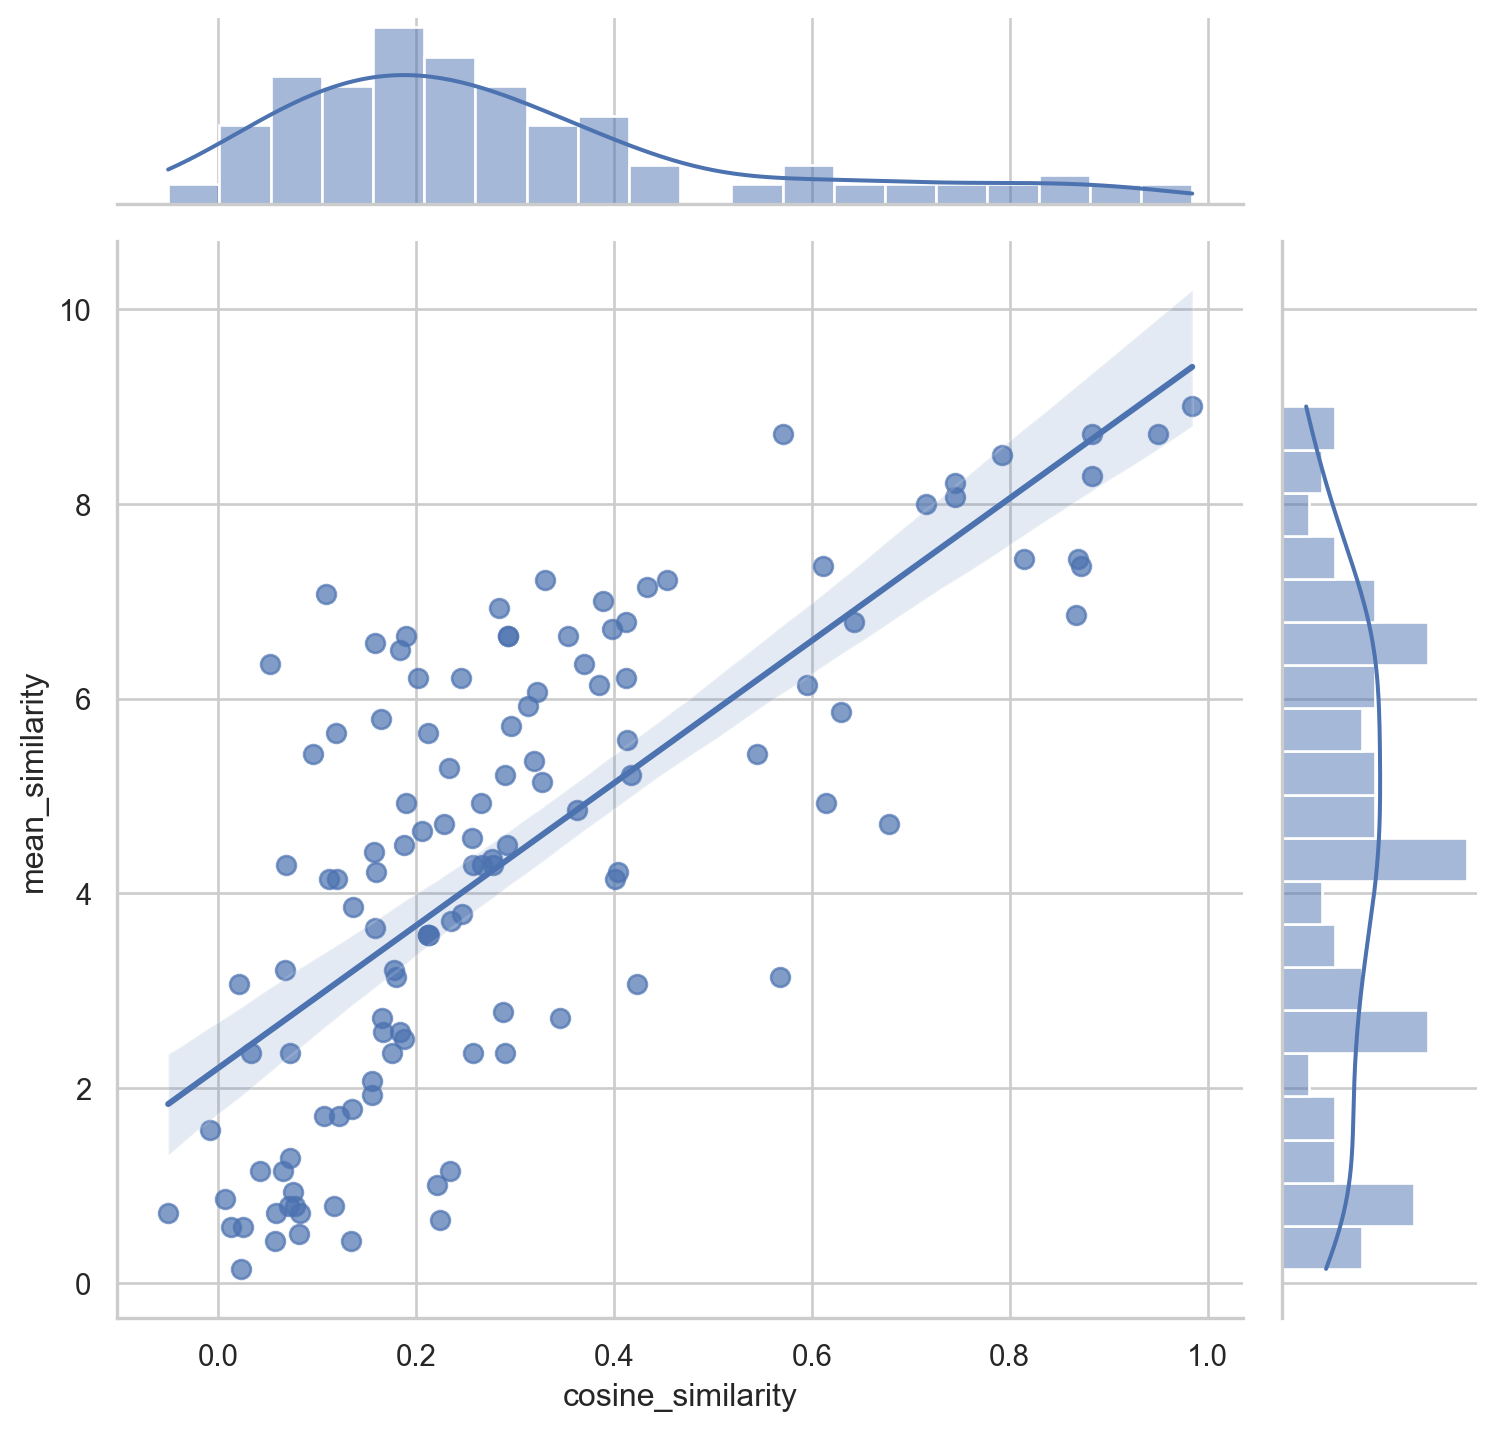
\includegraphics{06_ConceptSimilarity/ConceptNet_similarity_final_files/figure-pdf/cell-14-output-2.pdf}

The strong correlation (r=0.73) validates the use of ConceptNet
embeddings as a measure of conceptual similarity. In the next script
(\textbf{ADDREF?}), we will load it in together with our effort
features.

\begin{Shaded}
\begin{Highlighting}[]
\ImportTok{import}\NormalTok{ sys}
\BuiltInTok{print}\NormalTok{(sys.executable)}
\end{Highlighting}
\end{Shaded}

\begin{verbatim}
C:\Users\kadava\AppData\Local\anaconda3\envs\TSprocess\python.exe
\end{verbatim}

\bookmarksetup{startatroot}

\chapter{Summary}\label{summary}

\bookmarksetup{startatroot}

\chapter{Summary}\label{summary-1}

In summary, this book has no content whatsoever.

\bookmarksetup{startatroot}

\chapter{References}\label{references}

\bookmarksetup{startatroot}

\chapter*{References}\label{references-1}
\addcontentsline{toc}{chapter}{References}

\markboth{References}{References}

\phantomsection\label{refs}
\begin{CSLReferences}{1}{0}
\bibitem[\citeproctext]{ref-knuth84}
Knuth, Donald E. 1984. {``Literate Programming.''} \emph{Comput. J.} 27
(2): 97--111. \url{https://doi.org/10.1093/comjnl/27.2.97}.

\end{CSLReferences}



\end{document}
